\documentclass[a4paper,11pt,psamsfonts,reqno]{amsbook}

\usepackage[utf8]{inputenc}
\usepackage[T1]{fontenc}
\usepackage[english]{babel}
\usepackage{calc}
\usepackage{color}
\usepackage{float}
\usepackage{geometry}
\usepackage{microtype}
\usepackage{setspace}
\usepackage{graphicx}
\usepackage[colorlinks=true,urlcolor=blue]{hyperref}
\usepackage{longtable}
\usepackage{pdfpages}
\usepackage{amscd,amsmath,amssymb,amstext,amsthm}
\usepackage{braket}
\usepackage{mathpartir}
\usepackage{tikz}

\usetikzlibrary{cd}
\usetikzlibrary{patterns}
\usetikzlibrary{tqft}


\geometry{a4paper,left=20mm,right=20mm,top=20mm,bottom=20mm}
\onehalfspacing

\allowdisplaybreaks


\newcounter{prpcounter}


\newtheoremstyle{proposition}
{0pt}
{10pt}
{\normalfont}
{}
{\bfseries}
{}
{0.8em}
{\bfseries{\thmnumber{#2}\hspace{0.4em}\thmname{#1}\thmnote{\hspace{0.5em}(#3)}}}

\newtheoremstyle{proof}
{0pt}
{10pt}
{\normalfont}
{}
{\bfseries}
{}
{0.8em}
{\bfseries{\thmname{#1}\thmnote{\hspace{0.5em}(#3)}}}


\theoremstyle{proposition}
\newtheorem{prp}{Proposition}[prpcounter]
\newtheorem{con}[prp]{Conjecture}
\newtheorem{cor}[prp]{Corollary}
\newtheorem{cst}[prp]{Construction}
\newtheorem{exa}[prp]{Example}
\newtheorem{lem}[prp]{Lemma}
\newtheorem{rem}[prp]{Remark}
\newtheorem{thm}[prp]{Theorem}


\theoremstyle{proof}
\newtheorem{prf}{Proof}


\setcounter{tocdepth}{2}


\begin{document}

\title{Ordinary TQFTs and Close Encounters of the Higher Kind}
\author{SHTSoft.EU\footnote{\datename{ \today}}}
\maketitle
\tableofcontents


\input{macros.tex}


\chapter{Introduction}
\label{chap:intro}
\stepcounter{prpcounter}
%\nocite{f215dbd0}
%\nocite{cc6d78b5}
%\nocite{dfcdc48c}
%\nocite{8b5861fc}
%\nocite{00000001}
%\nocite{wiki-nlab0000}
%\nocite{wiki-pedia0en}
%
%
%%%
Whenever one aims to describe something it is important to have a good language or framework in which the description can be given. The right language can simplify the description and increase the understanding significantly and hence make for an improved reasoning. The development of a good mathematical framework in physics exemplifies this in an often amazing way. Coming up with new ideas for the mathematical language can give better insights in the physics to be described. In recent years it has come to light that category theory can provide a well-suited framework, especially in quantum field theory. While in general this is still in the beginnings, there is a special case for which quite some progress has been made, namely topological quantum field theories (TQFTs). These are interesting not only for physicists but also for mathematicians. Ordinary category theory is well-suited for describing ordinary TQFTs but one really aims to understand extended TQFTs and here higher categories come into play as a proper framework.\\
What we want to do in this work is to give an introduction to TQFTs, starting with ordinary TQFTs to get a feeling for what a TQFT looks like and then examine how one is led to extended TQFTs. As we want to address mathematicians and physicists alike, and in particular mathematical physicists, we moreover try to motivate the categorical definition of a TQFT from concepts which are more widespread in physics. Furthermore, our description of the ordinary category of cobordisms is rather thorough and we also try to make clear what higher cobordisms used for extended TQFTs are. This is often neglected a bit in the existing literature on the topic and should be helpful for the reader unfamiliar with these notions.
\\\\
Apart from some basic undergraduate math like linear algebra here and there it is necessary to know some basics of category theory - in particular categories, functors and natural transformations and moreover adjoints, limits and the idea of universality - in order to understand this text. Furthermore one should have a good idea of symmetric monoidal categories, but we will recall the definitions here and the reader unfamiliar with them possibly can get a basic understanding along the way.
\\
A good understanding of manifolds is also almost mandatory as we only give the basic definitions and results we need, which, of course, cannot replace a thorough introduction as given in some standard textbook. The same is true for the concept of fiber bundles, particularly principal bundles, vector bundles and their relation. Moreover, some knowledge about homotopy theory and also simplicial sets is very helpful, especially when it comes to higher categories. Yet, as our treatment of higher categories is rather informal, at least simplicial sets are not strictly needed for most of this work.
\\
A perfect reader is already familiar with the concept of higher categories since our treatment of them is not perfectly detailed (yet hopefully sufficient to be able to understand this text even without prior knowledge). Besides, such a perfect reader knows some singular homology, which is needed for parts of the concept of orientation, because we only give a short axiomatic description of homology in the appendix without providing intuition. Finally, a basic understanding of quantum field theory is helpful, at least from a physical point of view. We give a very rough overview of the main ideas to put this work in context and hopefully this is enough to be a good motivation to read on. To understand this motivation some basic knowledge about classical field theory and quantum mechanics is required. However, most of the text can be understood without any knowledge of quantum field theory and should still be interesting from a mathematical point of view.
\\
Much of these prerequisites is covered in \cite{00000001}, in particular the categorical parts. Just as done there we use Tarski-Grothendieck set theory as a foundation in order not to have to care about {\glqq}size issues{\grqq}. See \cite{00000001} for more on this. In fact, after reading this reference one should be sufficiently prepared to understand pretty much all of the present work. For the other concepts we refer to standard textbooks like \cite{8b5861fc} for basic homotopy theory\footnote{actually this is also sufficiently treated in \cite{00000001}} and homology or \cite{f215dbd0} for bundles. For quantum field theory from a mathematical perspective a good point to start is the nLab, \cite{wiki-nlab0000}, which also is a good first reference in general as is Wikipedia, \cite{wiki-pedia0en}. Every now and then there will be notions written in \textit{italic} style. These are notions which actually need a precise definition we do not provide because they are not central for the understanding or because we have given an informal description which is enough here. So, a reader who is unfamiliar with these notions should be able to read on even without a deeper understanding.
\\\\
Before starting with the main text we give an overview of quantum field theory in chapter \ref{chap:motqft} which should serve as a motivation from a physical point of view as already mentioned above.
\\
The main text is divided into two parts. The first part is about ordinary TQFTs. In chapter \ref{chap:prelim1} we start with recalling the necessary definitions for symmetric monoidal categories and dual objects. Afterwards we briefly discuss principal bundles and vector bundles and how they are related. Then we introduce the concept of orientation on manifolds for the reader unfamiliar with it. After these preliminaries we spend the subsequent chapter \ref{chap:defordtqft} on introducing the categories involved in the definition of a TQFT, the cobordism category and the category of vector spaces. We finish chapter \ref{chap:defordtqft} with finally defining ordinary TQFTs. As a short interlude in chapter \ref{chap:motpathint} we try to motivate this categorical definition from properties of the path integral which is widely used in quantum field theory in physics. In the final chapter \ref{CHAP:ALTCHARPROPS} of this part we are concerned with some basic statements about ordinary TQFTs. We start with giving an alternative characterization and then examine how to compare TQFTs. Afterwards we consider some basic general properties of TQFTs. Many of these things easily follow from purely categorical considerations.
\\
The second part is about extended TQFTs and the cobordism hypothesis which was originally stated by Baez and Dolan in \cite{cc6d78b5}. This part is essentially based on Lurie's expository paper \cite{dfcdc48c} about a precise formulation and a proof of the cobordism hypothesis. We start with some preliminaries in chapter \ref{chap:prelim2}, more precisely we give an informal introduction to higher categories and we introduce manifolds with corners and extended cobordisms. In chapter \ref{chap:lowdimtqft} we consider ordinary TQFTs of low dimension as a motivation for extended TQFTs. The following chapter \ref{chap:extcob} then is about extending the ordinary category of cobordisms to obtain a more sophisticated higher category of cobordisms. This is again done on an informal level as our treatment about higher categories was already informal. In the final chapter \ref{chap:formcobhyp} of this part we give a formulation of several versions of the cobordism hypothesis in the framework developed in the preceding chapters. We do not attempt for a description of the proof here as this is rather elaborated and we have neither the space and time nor the means to do this.
\\
After the main text we round off this work with a brief outlook in chapter \ref{chap:outlook}.
\\
The appendix includes a brief axiomatic introduction to homology, a sketch of the main idea of morse theory and moreover some of the tedious and little insightful parts of some proofs from chapter \ref{CHAP:ALTCHARPROPS} in the main part.
\\\\
We try to give a good intuition for the central ideas and still provide enough formal details to get a thorough understanding of the important parts. In some places we are more formal, for example in the orientation part especially when dealing with homology, but in other places, in particular when it comes to higher categories, we are quite informal, only trying to make clear what the idea is.
\\
In order to improve readability and comprehensibility some definitions are repeated here and there which, of course, comes at the cost of increased length. Moreover, the text is written in a rather decompressed way which considerably contributes to its length but hopefully makes it much easier to read.
\\
Definitions are given in the running text in \textbf{boldface} by phrases like {\glqq}formula such-and-such is called \textbf{name}{\grqq} or {\glqq}formula 1 is \textbf{name} if formula 2{\grqq}. Sometimes parts of the boldface text are written in parentheses which indicates that these parts are often left implicit in practice.
\\
Usually, statements are given in separate environments like lemma, theorem and corollary but minor statements are sometimes also given in the running text. If the statement is given in a separate environment then so is its proof which is closed with a $\Box$. For the statements in the running text the arguments for their proofs are also given in the running text. Sometimes proofs are only sketched or omitted altogether but usually there is a reference then where a more detailed proof can be found.
\\
Finally, there are several examples, often serving as illustrations but sometimes also as important parts of other statements. Mostly, examples are given in separate environments, too, on the one hand for later reference but on the other hand also for further structuring the text.




\section{Standard Notation}
\label{sec:notation}
%\nocite{00000001}
%%%
With respect to notation we generally follow mathematical convention. However, in order to make the text easier to read and for our convenience we fix some symbols for variables we often use so that we do not have to define the same symbol with the same meaning all the time. These symbols are given in the table at the end of this subsection. Thus if there appear undefined symbols in the text for which it is not immediately clear what they are supposed to mean the reader might have a look at this table. However, there may be more specifications in the text for such a symbol than those in the table, for example a manifold is often also compact.
\\
When we write phrases like {\glqq}we (usually/often) write{\grqq} then this means that the notation is fixed throughout the text. Besides, we often abuse notation a bit, for example by leaving some of the full notation implicit. For convenience we introduce the symbol $\doteq$ to do that. This means that we often write
\begin{align*}
  \text{abusive notation}
  &\doteq
  \text{full notation}
\end{align*}
indicating that we may also use the abusive notation instead of the full notation. Overall, we tried to use a consistent notation in the sense of choosing different symbol styles for different things like $\mathbf{boldface}$ symbols for categories. Last but not least, we mostly tried to keep our notation consistent with the notation in \cite{00000001}.
\begin{longtable}{cl}
  \hline
  Symbol
  &
  Meaning
  \\
  \hline
  \endhead
  \hline
  \endfoot
  $\mathbb{N}$
  &
  set of natural numbers with $0$
  \\[6pt]
  $\mathbb{N}^{\times}$
  &
  set of natural numbers without $0$
  \\[6pt]
  $k,m,n$
  &
  variables for elements of $\mathbb{N}$ or $\mathbb{N}^{\times}$
  \\[6pt]
  $\mathsf{J}$
  &
  variable for an index set
  \\[6pt]
  $\mathbf{C}$
  &
  variable for a category
  \\[6pt]
  ${_{n}}\mathbf{C}$
  &
  variable for an $n$-category
  \\[6pt]
  ${_{(\infty,n)}}\mathbf{C}$
  &
  variable for an $(\infty,n)$-category
  \\[6pt]
  $X$
  &
  variable for an object of $\mathbf{C}$, ${_{n}}\mathbf{C}$
  or ${_{(\infty,n)}}\mathbf{C}$
  \\[6pt]
  $X_{i}$
  &
  variables for objects of $\mathbf{C}$, ${_{n}}\mathbf{C}$
  or ${_{(\infty,n)}}\mathbf{C}$
  for all $i \in \lbrace 0,\ldots,9 \rbrace$
  \\[6pt]
  $f_{i_{1}i_{2}}$
  &
  variables for morphisms from $X_{i_{1}}$ to $X_{i_{2}}$
  for all $i_{1},i_{2} \in \lbrace 0,\ldots,9 \rbrace$
  \\[6pt]
  $\mathbf{C}_{a}$
  &
  variables for categories
  for $a \in \lbrace \alpha,\beta \rbrace$
  \\[6pt]
  ${_{n}}\mathbf{C}_{a}$
  &
  variables for $n$-categories
  for $a \in \lbrace \alpha,\beta \rbrace$
  \\[6pt]
  ${_{(\infty,n)}}\mathbf{C}_{a}$
  &
  variables for $(\infty,n)$-categories
  for $a \in \lbrace \alpha,\beta \rbrace$
  \\[6pt]
  $X^{a}$
  &
  variables for objects of $\mathbf{C}_{a}$, ${_{n}}\mathbf{C}_{a}$
  or ${_{(\infty,n)}}\mathbf{C}_{a}$
  for $a \in \lbrace \alpha,\beta \rbrace$
  \\[6pt]
  $X_{i}^{a}$
  &
  variables for objects of $\mathbf{C}_{a}$, ${_{n}}\mathbf{C}_{a}$
  or ${_{(\infty,n)}}\mathbf{C}_{a}$
  for $a \in \lbrace \alpha,\beta \rbrace$
  and all $i \in \lbrace 0,\ldots,9 \rbrace$
  \\[6pt]
  $f_{i_{1}i_{2}}^{a}$
  &
  variables for morphisms from $X_{i_{1}}^{a}$ to $X_{i_{2}}^{a}$
  for $a \in \lbrace \alpha,\beta \rbrace$
  and all $i_{1},i_{2} \in \lbrace 0,\ldots,9 \rbrace$
  \\[6pt]
  $F$
  &
  variable for a functor from $\mathbf{C}$ to $\mathbf{C}_{\alpha}$
  \\[6pt]
  $F_{i}$
  &
  variables for functors from $\mathbf{C}$ to $\mathbf{C}_{\alpha}$
  for all $i \in \lbrace 0,\ldots,9 \rbrace$
  \\[6pt]
  $F_{a_{1}a_{2}}$
  &
  variables for functors from $\mathbf{C}_{a_{1}}$ to $\mathbf{C}_{a_{2}}$
  for all $a_{1},a_{2} \in \lbrace \alpha,\beta \rbrace$
  \\[6pt]
  $Z$
  &
  variable for a TQFT
  \\[6pt]
  $S$
  &
  variable for a smooth manifold
  without boundary
  \\[6pt]
  $S_{i}$
  &
  variables for smooth manifolds
  without boundary
  for all $i \in \lbrace 0,\ldots,9 \rbrace$
  \\[6pt]
  $M$
  &
  variable for a smooth manifold
  possibly with boundary or corners
  \\[6pt]
  $M_{i}$
  &
  variables for smooth manifolds
  possibly with boundary or corners
  for all $i \in \lbrace 0,\ldots,9 \rbrace$
  \\[6pt]
  $V$
  &
  variable for a vector space
  \\[6pt]
  $V_{i}$
  &
  variables for vector spaces
  for all $i \in \lbrace 0,\ldots,9 \rbrace$
  \\
  \hline
\end{longtable}




\chapter{Motivation - An overview of QFT}
\label{chap:motqft}
\stepcounter{prpcounter}
%\nocite{00000001}
%\nocite{wiki-nlab0000}
%%%
Quantum field theory (QFT) is the framework in which fundamental processes in physics, especially in particle physics, are described today. However, it is not that easy to say what a QFT\footnote{note that the term quantum field theory can mean a single quantum field theory or the whole subject of quantum field theories (QFTs), but it should always be clear from the context what is meant} is as there is no canonical, generally agreed upon definition. Historically quantum field theory began with the description of the electromagnetic field in a more quantum kind of way by treating it as a collection of quantum harmonic oscillators. This was necessary because in ordinary, or relativistic\footnote{The Schr{\"o}dinger equation of ordinary QM is not compatible with special relativity since it treats time and space in a fundamentally different fashion. There is, however, a relativistic version of QM whose guiding equation is the Dirac equation which can be viewed as a relativistic improvement of the Schr{\"o}dinger equation.}, quantum mechanics (QM) the interaction of particles like electrons with the electromagnetic field is described semi-classically, i.e. the particles are treated in a quantum mechanical way but the electromagnetic field is treated classically, and this description is unable to capture the spontaneous emission of a photon by an excited\footnote{excited means that the particle is in a state with higher energy than the ground state which is the state of minimal energy} electron. The quantum mechanical description of the electromagnetic field indeed is able to account for spontaneous emission and led to the precursor of quantum electrodynamics (QED). This precursor is not really a QFT since at that time the material particles were viewed as eternal, which means that they cannot be created or destroyed, whereas photons were considered as excited states of the electromagnetic quantum field offering the possibility of their creation and destruction. But soon it was realized that material particles can be described by quantum fields in a similar way, so that, given enough energy, material particles can come into and out of existence, too, which is in contrast to QM where one deals with a fixed (usually small) number of particles. The description of electrons as a field finally led to QED, the first real QFT.
\\\\
So, QFT emerged from the attempt to combine classical field theory (CFT) with quantum mechanics in the context of special relativity. More generally, one also wants to consider curved spacetimes\footnote{we can think of spacetime as a Lorentzian manifold with a time-orientation, which roughly is a semi-Riemannian manifold with one dimension for time and the other dimensions for space in a proper sense} and not only Minkowski space, which is necessary for example to describe radiation of black holes. For a sketch of the basic idea which we aim to describe in the following this will not play much of a role. Note however that in the general case of curved spacetimes the concept of particles is generally not sensible anymore. Moreover, we should briefly talk about fields. Naively a field or field configuration or field history\footnote{a field configuration is sometimes rather understood as being defined only on space and not on spacetime, so field history is probably the better terminology} is a smooth function from spacetime to some other space, usually a manifold. Scalar fields, for example, have values in the field one considers, usually the real or complex numbers. In general, however, fields are not defined globally but rather in a local fashion which basically means that they are actual functions only on the local charts of spacetime. The principle of locality then says that the global fields should be determined by the local data. Yet, according to the gauge principle, one should not simply identify the local data in the overlapping region of two coordinate charts but there should be a gauge transformation connecting them. In this way one can capture topologically non-trivial global information. To properly describe this, one uses certain fiber bundles so that fields are really sections of fiber bundles. This will not play much of a role for the following (very basic) outline of QFT, at least not explicitly, and the reader is referred to \cite{00000001} for more on this.
\\\\
The basic idea in QFT is to start with a classical Lagrangian (density\footnote{the Lagrangian itself is actually often understood to be the volume integral of the Lagrangian density over space but for brevity we use the word Lagrangian for Lagrangian density}) $\mathcal{L}$ describing all the fields in a classical fashion. Remember that the Lagrangian is a real-valued function of the fields and their derivatives (usually only finitely many, e.g. only the first derivatives) and integrating $\mathcal{L}$ over spacetime yields the action (functional) of the system. There may be terms for a variety of fields in such a Lagrangian, that is, the Lagrangian generally is a finite sum
\begin{align*}
  \mathcal{L}
  &=
  \mathcal{L}_{1}
  +
  \mathcal{L}_{2}
  +
  \ldots
  +
  \mathcal{L}_{n}
\end{align*}
of different contributions. The term for the field of the electron\footnote{or other spin-$\frac{1}{2}$ fermions}, for example, comes from the Dirac field obtained by {\glqq}reinterpreting{\grqq} the general solution to the corresponding wave equation from relativistic QM, the Dirac equation, as a classical field. This means that the Euler-Lagrange equation for this term is exactly the Dirac equation. A scalar field is described by a term corresponding to the Klein-Gordon equation, another equation in relativistic QM. Vector fields, like the electromagnetic field, may be described using field strength tensors. In addition to these terms for free fields one needs terms for the interaction of the free fields to obtain realistic QFTs. These are usually appropriate products of the fields one intends to couple, multiplied with some coupling factor controlling the strength of the interaction. The Lagrangian thus is often written as
\begin{align*}
  \mathcal{L}
  &=
  \mathcal{L}_{\textrm{free}}
  +
  \mathcal{L}_{\textrm{int}}
\end{align*}
where $\mathcal{L}_{\textrm{free}}$ is the part for the free fields and $\mathcal{L}_{\textrm{int}}$ is the interaction part. An important way to obtain the correct interaction terms is by contemplating gauge symmetries of the system considered, which in terms of Lagrangians means that the Lagrangian is demanded to be invariant under certain gauge transformations. Such theories are called gauge theories. Starting, for example, with a free Dirac field for the electron one can obtain all other terms in the Lagrangian for QED by applying gauge theory with gauge group\footnote{this is basically the group of gauge transformations} $U(1)$. One important systematic way to obtain the correct terms in this way (especially for non-abelian gauge groups) is Yang-Mills theory. For a more accurate account on gauge theories we refer the reader to \cite{00000001}. Having all the terms in the Lagrangian one can obtain the Hamiltonian and the generalized momentum fields corresponding to the fields as usual by Legendre transformation.
\\
Now, the next step is to quantize the fields. To understand what quantization is supposed to mean let us first look at quantum mechanics. To arrive at quantum mechanics from classical mechanics in its Hamiltonian formulation, one intends to replace the classical observables\footnote{observables are meant to be the quantities that are measurable, at least in principle, like the position and momentum of a particle or the energy of the system} by operators on a Hilbert space of states of the quantum system. Observables in Hamiltionian mechanics are functions from the phase space to the real or complex numbers, so they form an algebra by using the pointwise operations, say $(A,\cdot)$ where $A$ is the underlying vector space and $\cdot$ the pointwise product. The phase space is the space of states in Hamiltonian mechanics and usually consists of all possible values of the generalized position and momentum variables of the system. Hence the obervables are functions of the generalized position and momentum variables and in particular these variables are turned into operators when doing the quantization. The obtained operators for position and momentum are then required to satisfy certain so-called canonical commutation relations - which encode the famous uncertainty principle - instead of the corresponding relations for the Poisson bracket of classical observables. Actually, one needs to impose other conditions in order to make this process of quantization sensible but the idea should be clear.
\\
The idea of quantization in QFT is basically the same. The fields and their corresponding momentum fields now become operators (at any spacetime point) acting on quantum states in a Hilbert space and they are again required to satisfy a field version of the canonical (anti\footnote{in the case of fermions one has anti-commutators instead of commutators}-)commutation relations. The Hamiltionian after quantization is then used to describe the time evolution of the system. Because of the canonical relations satisfied by the fields and momentum fields this quantization process is usually called canonical quantization. As some of the fields, like the Dirac field, have been obtained from quantum mechanical wave equations people sometimes also speak of second quantization (for historical reasons) when quantizing fields. Yet this is not really a good terminology because these fields were obtained by a reinterpretation of the wave functions of quantum wave equations as classical fields so that they are not quantized. For free field theories, i.e. without any interaction terms, one can indeed obtain QFTs using this idea. However, for interacting theories this is very difficult and only very simple examples have been worked out.
\\
There is an alternative approach to quantization using the so called path integral. For this approach the classical Lagrangian is used to calculate the action for the system. In classical Lagrangian mechanics the evolution of the system is obtained by examining where this action is stationary, i.e. where its functional derivative is zero. The idea of the path integral is then that not only the field which makes the action stationary determines how things evolve but one has to integrate over all fields, where each field is weighted with a phase factor determined by the action. This approach is often more convenient to work with, which is why it is often used by physicists today. Another advantage is that this approach is compatible with special relativity in an obvious way as opposed to the approach of canonical quantization for which this is not so obvious. However, there is a major problem: even though this approach yields physically sensible results, for most QFTs the path integral does not exist in a mathematically precise sense since there is no measure allowing to integrate over all fields.
\\\\
From a mathematical point of view there are essentially two approaches towards quantization. Before describing them we note that the phase space of a classical system is given by a sympletic manifold $(E,\omega)$, that is, a manifold $E$ together with a closed non-degenerate $2$-form $\omega$, called a sympletic form. This $2$-form determines a Lie bracket $\lbrace -,- \rbrace$, called the Poisson bracket, which controls the dynamics of the system and makes the commutative algebra of classical observables $(A,\cdot)$ into a Poisson algebra $(A,\cdot,\lbrace -,- \rbrace)$. This means in particular\footnote{there is another condition a Poisson algebra satisfies by definition which in some sense encodes the compatibility of the commutative product and the Poisson bracket} that the observables as a vector space together with the Poisson bracket form a Lie algebra $(A,\lbrace - ,- \rbrace)$. Now the two approaches for quantization are
\begin{itemize}
\item
Deformation quantization: this approach to quantization focuses on the algebra of observables and hence on the Heisenberg picture in which the dynamics of the system is encoded in the observables. The basic idea is to deform the commutative algebra of classical observables $(A,\cdot)$ by taking the same vector space but endowing it with a new product, denote it $\star$, which makes this vector space into a non-commutative algebra of quantum observables $(A,\star)$. The new product is required to have the property that the resulting commutator
\begin{align*}
  [O_{1},O_{2}]_{\star}
  &=
  O_{1}
  \star
  O_{2}
  -
  O_{2}
  \star
  O_{1}
\end{align*}
for two observables $O_{1},O_{2} \in A$ is to the {\glqq}first order{\grqq}, in an appropriate sense, determined by the Poisson bracket $\lbrace -,- \rbrace$. So, in some sense one deforms the commutative product to a non-commutative product in such a way that the commutator is a deformation of the Poisson bracket. Hence the name.
\\
Traditionally, and also often today, deformation quantization means formal deformation quantization which yields an algebra of formal power series $A[[\hbar]]$ in a formal parameter, usually denoted $\hbar$ which physically of course means Planck's constant. Thus the new product $\star$ is not really defined on the vector space $A$ of the original algebra but on the larger algebra of formal power series $A[[\hbar]]$ with coefficients in the original algebra. In the limit $\hbar \to 0$ this deformation should reproduce the original algebra. Formal deformation quantization actually corresponds to perturbative QFT (see below) so that the formal power series are usually cut off at some finite order in practice.
\\
A {\glqq}genuine{\grqq} quantization is not expected to yield just formal power series but actual functions. This is called strict deformation quantization or $C^{\ast}$-algebra deformation quantization because the resulting algebra is supposed to be a so-called $C^{\ast}$-algebra. 

\item
Geometric quantization: this approach focuses on the space of states and hence on the Schr{\"o}dinger picture in which the dynamics of the system is encoded in the states. Geometric quantization proceeds in two steps:
\begin{enumerate}
\item
The first step goes by the name prequantization. One chooses a certain line bundle\footnote{that is, a vector bundle of rank $1$} $L$ over $E$ with a connection\footnote{a connection basically says how the fibers of the vector bundle are connected and gives a way to identify fibers via a parallel transport which allows to do differentiation; for more on connections see e.g. \cite{00000001}}\,\footnote{more precisely one takes a line bundle with a bundle metric - hence one has an inner product for every fiber - and one takes a $U(1)$ connection - hence the corresponding parallel transport preserves the inner product} whose curvature $2$-form is basically the symplectic form $\omega$ of the given sympletic manifold $E$ representing the phase space of the classical system. This is called the prequantum line bundle. Under a certain condition for $\omega$ this is uniquely determined up to isomorphism. The (square-integrable) sections of this line bundle then form a Hilbert space\footnote{one can define an inner product on the space of sections of the line bundle by using the symplectic structure of the base manifold to define a volume form and hence do an integration; a section whose inner product with itself is finite is then called square-integrable} $H_{\textrm{p}}$ called the prequantum Hilbert space. One can also prequantize the classical observables by a map sending an observable to an operator on the prequantum Hilbert space in such a way that these operators satisfy commutator relations corresponding to the Poisson bracket relations of the corresponding classical observables. This involves the covariant derivative coming from the connection of the prequantum line bundle.

\item
However, the prequantum Hilbert space $H_{\textrm{p}}$ is too big to be the actual Hilbert space of quantum states. To cut it down one chooses a so called polarization which roughly is a way to divide the symplectic manifold $E$ representing the classical phase space into {\glqq}coordinates{\grqq} and {\glqq}momenta{\grqq}. The quantum Hilbert space $H \subset H_{\textrm{p}}$ then basically is the subspace of the prequantum Hilbert space consisting of those (square-integrable) sections of the prequantum line bundle $L$ which only depend on the coordinates and not on the momenta. Finally, one aims to take the classical observables to operators on this quantum Hilbert space $H$ in such a way that they satisfy appropriate commutator relations as can be done at the prequantum level. Unfortunately this is not possible for all observables on the quantum level, so things are a bit trickier here and one has to restrict to a certain subset of observables.
\end{enumerate}
\end{itemize}
In full generality the process of quantization is not very well-understood thus far. In fact, the (non-perturbative) quantization of Yang-Mills theory, which plays a fundamental role in the standard model of particle physics (SMP), is one of the famous {\glqq}Millenium Problems{\grqq}. But things become significantly easier when considering perturbative quantum field theory (pQFT). As much of the activity in physics is actually concerned with pQFT it is in order to briefly outline what the idea is.
\\\\
Perturbative QFT is meant to be an easier-to-handle approximation to full non-perturbative QFT. In pQFT one treats a part of the theory, usually the interaction part, as a small perturbation of the rest, usually the free fields. The time evolution in QFT is determined by an exponential of the Hamiltonian - or the Lagrangian in the path integral formulation - and the idea is to expand the interaction part\footnote{or more generally the part that represents the perturbation} of this exponential as a Taylor series in the coupling factor of the interaction which is assumed to be small. In this way the observables become (formal) power series\footnote{they are usually meant to be asymptotic expansions, i.e. they do not converge but still can be truncated at any finite order to yield controlled approximations to a function} in the coupling factor (and actually also in Planck's constant) and since this factor is supposed to be small it suffices to only consider low order terms to obtain good results.
\\
One is chiefly concerned with calculating so-called correlators in pQFT\footnote{and actually also in full QFT} which are basically (vacuum) expectation values\footnote{the vacuum expectation value can in principle be thought of as the average value for a measurement in the state with the lowest possible energy (vacuum)} of appropriate products of fields at some, potentially different, spacetime points. More precisely, one often deals with scattering amplitudes which are the probability amplitudes for scattering processes of particles or more generally of fields\footnote{in physics one mostly considers pQFT on Minkowski space so that the concept of particles as excitations of the fields makes sense}. One can think of this as a process where freely propagating fields in some state come in from the far past, then interact, i.e. scatter off each other, and then go off in some other state into the far future\footnote{in real applicatons the far past and far future are not that far on a classical level but compared to the {\glqq}time scale{\grqq} of the interaction this is a good approximation}. The scattering amplitudes are organized in the so called S-matrix which is then used to calculate numerical predictions - such as scattering cross sections - and is pretty much the key object of perturbative QFT. The scattering cross sections can be measured in scattering experiments, as done e.g. at the LHC particle accelerator, which are the main source of experimental verification of quantum field theory, or more particularly the SMP, today. Indeed, the predictions made with the help of perturbative methods about the SMP are in agreement with experiment to a (sometimes very) good precision. Due to the perturbative nature of the theory the S-matrix can be expressed as a sum over elementary processes, that is, specific ways of interaction. This leads to the famous Feynman diagrams governed by the Feynman rules.
\\
However, these computations, as physicists often do them, may lead to infinite values ({\glqq}divergences{\grqq}) of some quantities which is why one has to apply a process called renormalization. The problem basically is that there are some interactions that are not accounted for by the perturbative approach and thus some corrections are necessary. Moreover, physicists often resort to the path integral when doing calculations, which, as said above, cannot be defined rigorously in most cases. But there also is a mathematically rigorous formulation of pQFT properly treating these problems. The main idea is to focus on the S-matrix and to axiomatize how it should behave. The key property is called causal additivity and basically means that all effects caused in some spacetime region must be in the causal future of that region. Therefore this rigorous formulation of pQFT goes by the name causal perturbation theory. There also is a slight refinement called perturbative AQFT (pAQFT) where the observables are organized in such a way that they satisfy a variation of the Haag-Kastler axioms, which are an attempt to axiomatize QFT in general (see below), hence the name. This is in fact a rigorous formulation of perturbative QFT on Minkowski space, justifying often-used tools such as the Feynman diagrams. There are other equivalent rigorous formulations for pQFT on Minkowski space but the above approach by pAQFT has the advantage that it easily generalizes to more general curved spacetimes, at least to globally hyperbolic spacetimes which are an important subclass. This generalization is now called locally covariant perturbative AQFT (lcpAQFT). While mathematically precise and well motivated by heuristics of the path integral and also by experimental confirmation it seems desirable, at least from a physical point of view, that one can derive these constructions by some kind of quantization. As it has turned out quite recently this is indeed the case for (at least parts of) lcpAQFT, specifically by using some kind of formal deformation quantization called Fedosov deformation quantization. A (very) comprehensive introduction to lcpAQFT is given in the article \href{https://ncatlab.org/nlab/show/geometry+of+physics+--+perturbative+quantum+field+theory}{geometry of physics - perturbative quantum field theory} in \cite{wiki-nlab0000}. Now, apart from only being perturbative, there is basically only one problem left with lcpAQFT, namely when it comes to gauge theory on curved spacetimes one of the axioms encoding locality breaks. But there already is a proposed solution called homotopical AQFT where one passes to so called homotopical algebras of observables. But this is still in the making.
\\\\
While pQFT is comparatively well understood, though already quite involved mathematically, there are also non-perturbative effects (known e.g. from computer simulations or experiment) which cannot be captured with perturbative methods. A notable example is the confinement of quarks in quantum chromodynamics (QCD) at low energy. For low energies the coupling factor in QCD becomes large so that perturbation theory cannot be expected to be a good approximation anymore. An important keyword for non-perturbative effects is \textit{instantons}. These encode topologically non-trivial information of fields which may be a source for non-perturbative effects. There are methods like resurgence theory trying to capture non-perturbative effects in pQFT but it is far from clear whether this works. Thus a rigorous understanding of pQFT is only a step towards understanding full non-perturbative QFT.
\\
Non-perturbative QFT has remained much more elusive than its perturbative approximation, especially when it comes to quantization. As already mentioned above quantization of full QFT is currently not very well understood. Indeed, the only examples constructed satisfying the axioms of an axiomatization of QFT so far are toy models in that they do not incorporate interactions or are on spacetimes of dimension less than $4$. But what does an axiomatization of QFT look like? There are two main approaches for the axiomatization and formalization of QFT and they go by the names algebraic quantum field theory (AQFT) and functorial quantum field theory (FQFT).
\begin{itemize}
\item
AQFT focuses on the observables and thus can be viewed as an axiomatization of the Heisenberg picture. This approach is more widely considered among mathematical physicists. The main idea is to assign (usually $C^{\ast}$-)algebras of observables to certain patches of spacetime in a consistent way, meaning more precisely that they form a so called local net of  observables which is characterized by the Haag-Kastler axioms. In literature the axioms vary a bit but the assignment is always encoded in a presheaf and one of the main axioms is causal locality, basically meaning that observables defined on spacelike-seperated regions of spacetime commute with each other. We do not want to go into further detail here.

\item
FQFT focuses on the quantum states and thus can be viewed as an axiomatization of the Schr{\"o}dinger picture. This is the more recent approach. The main idea is to assign
\begin{itemize}
\item
a vector space $Z(S)$ (possibly a Hilbert space) of quantum states to every codimension-$1$ slice $S$ of spacetime representing space

\item
a linear operator $Z(M) \colon Z(S_{1}) \to Z(S_{2})$ between state spaces - thought of as the time evolution operator - to any (part of) spacetime $M$ which is a cobordism between the spatial slices $S_{1},S_{2}$ corresponding to the state spaces $Z(S_{1}),Z(S_{2})$; such a cobordism $M$ can be thought of as a manifold whose boundary consists of two parts, one for each of the spatial slices $S_{1}$ and $S_{2}$
\end{itemize}
This assignment is required to satisfy certain properties physicists expect the path integral to have, so that one can think of FQFT in some sense as axiomatizing the path integral yet without saying what the integration really is. These properties can be encoded by demanding the assignment to be a functor $Z$ from the category of cobordisms to the category of vector spaces. We will motivate this a little further in a later chapter.
\\
However, there is a problem with these axioms, namely that they break so called general covariance because spacetime is split into space and time which is not to be expected from a {\glqq}reasonable{\grqq} physical theory. What one would rather expect is that it is possible to {\glqq}propagate{\grqq} in spatial directions just as in time direction. Thus one has to consider not only submanifolds of spacetime of codimension $1$ but also of higher codimension. This is what is done in extended FQFT where one considers an extended category of cobordisms which contains manifolds of higher codimensions and hence is naturally cast in the language of higher categories. An extended FQFT is a higher functor from this higher category of cobordisms to an appropriate higher category of vector spaces, though it does not really seem to be clear yet what the {\glqq}correct{\grqq} higher category of vector spaces is. As this is a more local description - in fact corresponding to the locality a QFT is expected to have - it sometimes also goes by the name local FQFT.
\end{itemize}
In principle FQFT and AQFT should describe the same thing from different viewpoints, so they should be dual to each other just as algebra and geometry are dual to each other\footnote{the keyword here is Isbell duality}. In special cases this has already been made precise but both FQFT and AQFT are still in progress and so is their precise relation.
\\\\
A special case of FQFT for which there has been quite some progress and from which the idea of FQFT originally arose is topological QFT (TQFT). We will focus on this special case in this work. Basically, a QFT is called topological if the essential things like observables do not depend on the metric of the spacetime. Thus the manifolds in the cobordism category are not equipped with a metric (or other non-topological structure). On Minkowski space TQFTs are not very interesting because Minkowski space is contractible, that is, topologically trivial. Therefore one is usually concerned with more general curved spacetimes here. A notable example of TQFT is Chern-Simons theory which has become kind of a poster-child of (extended) TQFT. Potential applications of TQFT are topological insulators, the quantum Hall effect and topological quantum computing, but there remains much to be understood. Moreover, there is a classification result for TQFTs, which also is of considerable mathematical importance, namely the cobordism hypothesis. This is rather involved and a semi-formal formulation of the cobordism hypothesis will be at the end of our text.
\\\\
A good first mathematical reference for many of the notions in the above overview of QFT are the corresponding articles in \cite{wiki-nlab0000} and subsequently the references given there.





\part{Ordinary TQFTs}
\label{part:ordinary}
This first part is about ordinary TQFTs as first brought up in (almost) the axiomatization considered here by Atiyah in 1988. The description is given in the framework of ordinary categories or more precisely symmetric monoidal categories.
\\\\
The part is divided into four chapters starting with some preliminaries in chapter \ref{chap:prelim1} which are needed in the subsequent chapters of this and partly also of the second part. The next chapter, chapter \ref{chap:defordtqft}, is about the definition of TQFTs in categorical terms. In the following chapter \ref{chap:motpathint} we want to motivate this categorical definition from a formulation of QFT which is more widely used among physicists, the path integral. In the final chapter \ref{CHAP:ALTCHARPROPS} of this part we then consider some basic statements which hold true for any ordinary TQFT.
\\\\
The objective of this part is to give an introduction to ordinary TQFTs and convey some intuition for them. So, the reader who does not know about the subject should become familiar with ordinary TQFTs in the course of this part.





\chapter{Preliminaries}
\label{chap:prelim1}
\stepcounter{prpcounter}
%\nocite{00000001}
%%%
Let us start with the preliminaries of this part. In section \ref{sec:smoncatdual} we first recall the definitions of symmetric monoidal categories and dual objects. We do not give intuition here but the careful reader might notice that (symmetric) monoidal categories are a categorification of (commutative) monoids. The unexperienced reader may have a look at \cite{00000001} for more on this. Then in section \ref{sec:bundles} we briefly discuss some basics of bundles, particularly principal bundles, vector bundles and how they are related. The final section \ref{sec:orient} of this chapter is dedicated to the concept of orientation of manifolds. This is needed for one of the categories discussed in the definition of ordinary TQFTs, namely the category of cobordisms. We will usually deal with smooth manifolds, yet as we will also touch on oriented topological manifolds, and maybe for a better understanding of the concept altogether, we also consider orientability for topological manifolds. To properly understand orientation in this more general setting we need some basics of (singular) homology. The latter is briefly introduced in the appendix, though without giving proofs or intuition.


\section{Symmetric Monoidal Categories and Dual Objects}
\label{sec:smoncatdual}
%\nocite{e837ef86}
%\nocite{5175de60}
%\nocite{00000001}
%%%
As we will be concernded with symmetric monoidal categories and dual objects all the time here, we briefly want to recall the definitions as given, for example, in \cite{00000001}. A set $\mathcal{M}_{\mathbf{C}}$ is a \textbf{monoidal category} if it is a $6$-tuple
\begin{align*}
  \left(
    \mathbf{C},
    \otimes,
    \mathsf{A},
    1,
    \mathsf{L},
    \mathsf{R}
  \right)
\end{align*}
consisting of
\begin{enumerate}
\item[(1)]
a category $\mathbf{C}$
\item[(2)]
a functor
\begin{align*}
  \cdot
  \otimes
  \cdot
  \doteq
  \otimes
  \colon
  \mathbf{C}
  \times
  \mathbf{C}
  &\rightarrow
  \mathbf{C}
\end{align*}
\item[(3)]
for the functors
\begin{align*}
  \left(
    \cdot
    \otimes
    \cdot
  \right)
  \otimes
  \cdot
  \colon
  \mathbf{C}
  \times
  \mathbf{C}
  \times
  \mathbf{C}
  &\rightarrow
  \mathbf{C}
  \\
  (X_{1},X_{2},X_{3})
  &\mapsto
  \otimes(\otimes(X_{1},X_{2}),X_{3})
  \\
  (f_{12},f_{34},f_{56})
  &\mapsto
  \otimes(\otimes(f_{12},f_{34}),f_{56})
  \\\\
  \cdot
  \otimes
  \left(
    \cdot
    \otimes
    \cdot
  \right)
  \colon
  \mathbf{C}
  \times
  \mathbf{C}
  \times
  \mathbf{C}
  &\rightarrow
  \mathbf{C}
  \\
  (X_{1},X_{2},X_{3})
  &\mapsto
  \otimes(X_{1},\otimes(X_{2},X_{3}))
  \\
  (f_{12},f_{34},f_{56})
  &\mapsto
  \otimes(f_{12},\otimes(f_{34},f_{56}))
\end{align*}
a natural isomorphism
\begin{align*}
  \mathsf{A}
  \colon
  \left(
    \cdot
    \otimes
    \cdot
  \right)
  \otimes
  \cdot
  &\Rightarrow
  \cdot
  \otimes
  \left(
    \cdot
    \otimes
    \cdot
  \right)
\end{align*}
\item[(4)]
an object\footnote{this is not to be confused with terminal objects, though sometimes they coincide} $1$ of $\mathrm{ob}_{\mathbf{C}}$
\item[(5)]
for the functor
\begin{align*}
  \otimes(1,\cdot)
  \colon
  \mathbf{C}
  &\rightarrow
  \mathbf{C}
  \\
  X
  &\mapsto
  \otimes(1,X)
  \\
  f_{12}
  &\mapsto
  \otimes(\mathrm{id}_{1},f_{12})
\end{align*}
a natural isomorphism
\begin{align*}
  \mathsf{L}
  \colon
  \otimes(1,\cdot)
  &\Rightarrow
  \mathrm{id}_{\mathbf{C}}
\end{align*}
\item[(6)]
for the functor
\begin{align*}
  \otimes(\cdot,1)
  \colon
  \mathbf{C}
  &\rightarrow
  \mathbf{C}
  \\
  X
  &\mapsto
  \otimes(X,1)
  \\
  f_{12}
  &\mapsto
  \otimes(f_{12},\mathrm{id}_{1})
\end{align*}
a natural isomorphism
\begin{align*}
  \mathsf{R}
  \colon
  \otimes(\cdot,1)
  &\Rightarrow
  \mathrm{id}_{\mathbf{C}}
\end{align*}
\end{enumerate}
such that
\begin{enumerate}
\item[(MC1)]
the diagram
\begin{equation*}
\begin{tikzcd}[row sep=3.5em,column sep=0.4em]
  &
  (X_{1} \otimes X_{2})
  \otimes
  (X_{3} \otimes X_{4})
  \arrow{dr}{\mathsf{A}(X_{1},X_{2},X_{3} \otimes X_{4})}
  &
  \\
  \left(
    (X_{1} \otimes X_{2})
    \otimes
    X_{3}
  \right)
  \otimes
  X_{4}
  \arrow{ur}{\mathsf{A}(X_{1} \otimes X_{2},X_{3},X_{4})}
  \arrow[swap]{d}{\mathsf{A}(X_{1},X_{2},X_{3}) \otimes \mathrm{id}_{X_{4}}}
  &
  &
  X_{1}
  \otimes
  \left(
    X_{2}
    \otimes
    (X_{3} \otimes X_{4})
  \right)
  \\
  \left(
    X_{1}
    \otimes
    (X_{2} \otimes X_{3})
  \right)
  \otimes
  X_{4}
  \arrow{rr}{\mathsf{A}(X_{1},X_{2} \otimes X_{3},X_{4})}
  &
  &
  X_{1}
  \otimes
  \left(
    (X_{2} \otimes X_{3})
    \otimes
    X_{4}
  \right)
  \arrow[swap]{u}{\mathrm{id}_{X_{1}} \otimes \mathsf{A}(X_{2},X_{3},X_{4})}
\end{tikzcd}
\end{equation*}
commutes
\item[(MC2)]
the diagram
\begin{equation*}
\begin{tikzcd}[sep=large]
  (X_{1} \otimes 1)
  \otimes
  X_{2}
  \arrow{rr}{\mathsf{A}(X_{1},1,X_{2})}
  \arrow[swap]{dr}{\mathsf{R}(X_{1}) \otimes \mathrm{id}_{X_{2}}}
  &
  &
  X_{1}
  \otimes
  (1 \otimes X_{2})
  \arrow{dl}{\mathrm{id}_{X_{1}} \otimes \mathsf{L}(X_{2})}
  \\
  &
  X_{1}
  \otimes
  X_{2}
  &
\end{tikzcd}
\end{equation*}
commutes
\end{enumerate}
The sets given by the coordinates of a monoidal category
\begin{align*}
  \mathcal{M}_{\mathbf{C}}
  &=
  \left(
    \mathbf{C},
    \otimes,
    \mathsf{A},
    1,
    \mathsf{L},
    \mathsf{R}
  \right)
\end{align*}
have names in their own right.
\begin{enumerate}
\item[(1)]
$\mathbf{C}$ is called the \textbf{underlying category (in $\mathcal{M}_{\mathbf{C}}$)}
\item[(2)]
$\otimes$ is called the \textbf{tensor product (in $\mathcal{M}_{\mathbf{C}}$)}
\item[(3)]
$\mathsf{A}$ is called the \textbf{associator (in $\mathcal{M}_{\mathbf{C}}$)}
\item[(4)]
$1$ is called the \textbf{unit object (in $\mathcal{M}_{\mathbf{C}}$)}
\item[(5)]
$\mathsf{L}$ is called the \textbf{left unit law (in $\mathcal{M}_{\mathbf{C}}$)}
\item[(6)]
$\mathsf{R}$ is called the \textbf{right unit law (in $\mathcal{M}_{\mathbf{C}}$)}
\end{enumerate}
In a tensor product $X_{1} \otimes X_{2}$ we sometimes call $X_{1}$ and $X_{2}$ the tensor factors and sometimes call $X_{1} \otimes X_{2}$ the tensoring of $X_{1}$ and $X_{2}$. For the monoidal category property (MC1) we also say that the \textbf{pentagon equation (in $\mathcal{M}_{\mathbf{C}}$) holds} and for the monoidal category property (MC2) we say that the \textbf{triangle equation (in $\mathcal{M}_{\mathbf{C}}$) holds}. That these coherence conditions suffice in order to treat the associators and unit laws in the usual way, meaning that basically it does not matter how we reassociate an expression and where we apply the unit laws, is guaranteed by Mac Lane's coherence theorem which can be found in his category book \cite{e837ef86} or various other sources like \cite{5175de60}. This follows from, and sometimes is interchangably used with, Mac Lane's stricification theorem which states that every monoidal category is monoidally equivalent (see below) to a strict monoidal category, where strict means that the associator and unit laws all are identities. Due to these theorems it mostly suffices to consder strict monoidal categories.
\\
Next we consider monoidal functors. Let
\begin{align*}
  \mathcal{M}_{\mathbf{C}_{\alpha}}
  &=
  \left(
    \mathbf{C}_{\alpha},
    \otimes_{\alpha},
    \mathsf{A}_{\alpha},
    1_{\alpha},
    \mathsf{L}_{\alpha},
    \mathsf{R}_{\alpha}
  \right)
\end{align*}
another monoidal category. A set $\mathcal{M}_{F}$ is a \textbf{lax monoidal functor (from $\mathcal{M}_{\mathbf{C}}$ to $\mathcal{M}_{\mathbf{C}_{\alpha}}$)} if it is a $3$-tuple
\begin{align*}
  F
  \doteq
  \left(
    F,
    \mathsf{H},
    \Phi
  \right)
\end{align*}
consisting of a functor $F$ from $\mathbf{C}$ to $\mathbf{C}_{\alpha}$, a natural transformation
\begin{align*}
  \mathsf{H}
  \colon
  \otimes_{\alpha}
  \circ
  \left(
    F
    \times
    F
  \right)
  &\Rightarrow
  F
  \circ
  \otimes
\end{align*}
and a morphism
\begin{align*}
  \Phi
  &\in
  \mathrm{mor}_{\mathbf{C}_{\alpha}}(1_{\alpha},F(1))
\end{align*}
such that
\begin{enumerate}
\item[(MF1)]
the diagram
\begin{equation*}
\begin{tikzcd}[row sep=3em, column sep=9em]
  (F(X_{1}) \otimes_{\alpha} F(X_{2}))
  \otimes_{\alpha}
  F(X_{3})
  \arrow{r}{\mathsf{A}_{\alpha}(F(X_{1}),F(X_{2}),F(X_{3}))}
  \arrow[swap]{d}{\mathsf{H}(X_{1},X_{2})\otimes_{\alpha}\mathrm{id}_{F(X_{3})}}
  &
  F(X_{1})
  \otimes_{\alpha}
  (F(X_{2}) \otimes_{\alpha} F(X_{3}))
  \arrow{d}{\mathrm{id}_{F(X_{1})} \otimes_{\alpha} \mathsf{H}(X_{2},X_{3})}
  \\
  F(X_{1} \otimes X_{2})
  \otimes_{\alpha}
  F(X_{3})
  \arrow[swap]{d}{\mathsf{H}(X_{1} \otimes X_{2},X_{3})}
  &
  F(X_{1})
  \otimes_{\alpha}
  F(X_{2} \otimes X_{3})
  \arrow{d}{\mathsf{H}(X_{1},X_{2} \otimes X_{3})}
  \\
  F
  \left(
    (X_{1} \otimes X_{2})
    \otimes
    X_{3}
  \right)
  \arrow{r}{F(\mathsf{A}(X_{1},X_{2},X_{3}))}
  &
  F
  \left(
    X_{1}
    \otimes
    (X_{2} \otimes X_{3})
  \right)
\end{tikzcd}
\end{equation*}
commutes
\item[(MF2)]
the diagrams
\begin{equation*}
\begin{tikzcd}[sep=large]
  1_{\alpha}
  \otimes_{\alpha}
  F(X)
  \arrow{r}{\mathsf{L}_{\alpha}(F(X))}
  \arrow[swap]{d}{\Phi \otimes_{\alpha} \mathrm{id}_{F(X)}}
  &
  F(X)
  \\
  F(1)
  \otimes_{\alpha}
  F(X)
  \arrow{r}{\mathsf{H}(1,X)}
  &
  F(1 \otimes X)
  \arrow[swap]{u}{F(\mathsf{L}(X))}
\end{tikzcd}
\end{equation*}
and
\begin{equation*}
\begin{tikzcd}[sep=large]
  F(X)
  \otimes_{\alpha}
  1_{\alpha}
  \arrow{r}{\mathsf{R}_{\alpha}(F(X))}
  \arrow[swap]{d}{\mathrm{id}_{F(X)} \otimes_{\alpha} \Phi}
  &
  F(X)
  \\
  F(X)
  \otimes_{\alpha}
  F(1)
  \arrow{r}{\mathsf{H}(X,1)}
  &
  F(X \otimes 1)
  \arrow[swap]{u}{F(\mathsf{R}(X))}
\end{tikzcd}
\end{equation*}
commute
\end{enumerate}
The monoidal functor properties (MF1) and (MF2) express that the functor $F$ is compatible with the corresponding monoidal structures. A lax monoidal functor $(F,\mathsf{H},\Phi)$ is called\footnote{some authors use strong monoidal functor here but we do not since this is our standard case} \textbf{monoidal functor} if both $\mathsf{H}$ and $\Phi$ are isomorphisms while it is called \textbf{strict monoidal functor} if both are identities.
\\
Now we come to monoidal natural transformations. Given monoidal functors
\begin{align*}
  \mathcal{M}_{F_{1}}
  =
  \left(
    F_{1},
    \mathsf{H}_{1},
    \Phi_{1}
  \right)
  \qquad
  &\text{and}
  \qquad
  \mathcal{M}_{F_{2}}
  =
  \left(
    F_{2},
    \mathsf{H}_{2},
    \Phi_{2}
  \right)
\end{align*}
a natural transformation $\mathsf{T}_{12}$ from $F_{1}$ to $F_{2}$ is \textbf{monoidal (w.r.t $\mathcal{M}_{F_{1}}$ and $\mathcal{M}_{F_{2}}$)} if
\begin{enumerate}
\item[(MT1)]
the diagram
\begin{equation*}
\begin{tikzcd}[row sep=large,column sep=8em]
  F_{1}(X_{1})
  \otimes_{\alpha}
  F_{1}(X_{2})
  \arrow{r}{\mathsf{T}_{12}(X_{1}) \otimes_{\alpha} \mathsf{T}_{12}(X_{2})}
  \arrow[swap]{d}{\mathsf{H}_{1}(X_{1},X_{2})}
  &
  F_{2}(X_{1})
  \otimes_{\alpha}
  F_{2}(X_{2})
  \arrow{d}{\mathsf{H}_{2}(X_{1},X_{2})}
  \\
  F_{1}(X_{1} \otimes X_{2})
  \arrow{r}{\mathsf{T}_{12}(X_{1} \otimes X_{2})}
  &
  F_{2}(X_{1} \otimes X_{2})
\end{tikzcd}
\end{equation*}
commutes
\item[(MT2)]
the diagram
\begin{equation*}
\begin{tikzcd}[sep=large]
  1_{\alpha}
  \arrow{dr}{\Phi_{2}}
  \arrow{d}[swap]{\Phi_{1}}
  &
  \\
  F_{1}(1)
  \arrow{r}{\mathsf{T}_{12}(1)}
  &
  F_{2}(1)
\end{tikzcd}
\end{equation*}
commutes
\end{enumerate}
Again, the monoidal natural transformation properties (MT1) and (MT2) obviously express compatibility with the involved structures. To define equivalence of monoidal categories note that the identity functor and the composition of monoidal functors are monoidal. Hence $\mathcal{M}_{F_{\alpha\beta}}$ is a \textbf{monoidal equivalence (from $\mathcal{M}_{\mathbf{C}_{\alpha}}$ to $\mathcal{M}_{\mathbf{C}_{\beta}}$)} if there is $\mathcal{M}_{F_{\beta\alpha}}$ such that there exist monoidal natural isomorphisms from $F_{\beta\alpha} \circ F_{\alpha\beta}$ to $\mathrm{id}_{\mathbf{C_{\alpha}}}$ and from $F_{\alpha\beta} \circ F_{\beta\alpha} $ to $\mathrm{id}_{\mathbf{C_{\beta}}}$ respectively.
\\\\
The next step is to add a kind of commutativity for the tensor product of a monoidal category. A set $\mathcal{B}_{\mathbf{C}}$ is a \textbf{braided monoidal category} if it is a tuple $(\mathcal{M}_{\mathbf{C}},\mathsf{B})$ consisting of a monoidal category $\mathcal{M}_{\mathbf{C}}$ and for the functor
\begin{align*}
  \otimes_{\textrm{B}}
  \colon
  \mathbf{C}
  \times
  \mathbf{C}
  &\rightarrow
  \mathbf{C}
  \\
  (X_{1},X_{2})
  &\mapsto
  \otimes(X_{2},X_{1})
  \\
  (f_{12},f_{34})
  &\mapsto
  \otimes(f_{34},f_{12})
\end{align*}
a natural isomorphism
\begin{align*}
  \mathsf{B}
  \colon
  \otimes
  &\Rightarrow
  \otimes_{\textrm{B}}
\end{align*}
such that
\begin{enumerate}
\item[(BC1)]
the diagram
\begin{equation*}
\begin{tikzcd}[row sep=huge,column sep=8em]
  (X_{2} \otimes X_{1})
  \otimes
  X_{3}
  \arrow{r}{\mathsf{A}(X_{2},X_{1},X_{3})}
  &
  X_{2}
  \otimes
  (X_{1} \otimes X_{3})
  \arrow{d}{\mathrm{id}_{X_{2}} \otimes \mathsf{B}(X_{1},X_{3})}
  \\
  (X_{1} \otimes X_{2})
  \otimes
  X_{3}
  \arrow{u}{\mathsf{B}(X_{2},X_{1}) \otimes \mathrm{id}_{X_{3}}}
  &
  X_{2}
  \otimes
  (X_{3} \otimes X_{1})
  \arrow{d}{\mathsf{A}^{-1}(X_{2},X_{3},X_{1})}
  \\
  X_{1}
  \otimes
  (X_{2} \otimes X_{3})
  \arrow{u}{\mathsf{A}^{-1}(X_{1},X_{2},X_{3})}
  \arrow{r}{\mathsf{B}(X_{1},X_{2} \otimes X_{3})}
  &
  (X_{2} \otimes X_{3})
  \otimes
  X_{1}
\end{tikzcd}
\end{equation*}
commutes
\item[(BC2)]
the diagram
\begin{equation*}
\begin{tikzcd}[row sep=huge,column sep=8em]
  X_{1}
  \otimes
  (X_{3} \otimes X_{2})
  \arrow{r}{\mathsf{A}^{-1}(X_{1},X_{3},X_{2})}
  &
  (X_{1} \otimes X_{3})
  \otimes
  X_{2}
  \arrow{d}{\mathsf{B}(X_{1},X_{3}) \otimes \mathrm{id}_{X_{2}}}
  \\
  X_{1}
  \otimes
  (X_{2} \otimes X_{3})
  \arrow{u}{\mathrm{id_{X_{1}}} \otimes \mathsf{B}(X_{2},X_{3})}
  &
  (X_{3} \otimes X_{1})
  \otimes
  X_{2}
  \arrow{d}{\mathsf{A}(X_{3},X_{1},X_{2})}
  \\
  (X_{1} \otimes X_{2})
  \otimes
  X_{3}
  \arrow{u}{\mathsf{A}(X_{1},X_{2},X_{3})}
  \arrow{r}{\mathsf{B}(X_{1} \otimes X_{2},X_{3})}
  &
  X_{3}
  \otimes
  (X_{1} \otimes X_{2})
\end{tikzcd}
\end{equation*}
commutes
\end{enumerate}
For the braided monoidal category properties (BC1) and (BC2) we also say that the \textbf{hexagon equations (in $\mathcal{B}_{\mathbf{C}}$) hold}. Note that these equations express that when given three tensor factors we can either interchange two of them with the other at once or we can do it one after the other. The coordinate $\mathsf{B}$ in $\mathcal{B}_{\mathbf{C}}$ is called \textbf{braiding} and there is a case of special interest. Namely, a braided monoidal category $\mathcal{B}_{\mathbf{C}}$ is \textbf{symmetric} if
\begin{align*}
  \mathsf{B}(X_{2},X_{1})
  \circ
  \mathsf{B}(X_{1},X_{2})
  &=
  \mathrm{id}_{\otimes}(X_{1},X_{2})
\end{align*}
holds for all $X_{1}$ and $X_{2}$. We usually say, a bit inaccurately, symmetric monoidal category instead of symmetric braided monoidal category.
\\
Of course, one can define functors respecting these extra pieces of structure. A set $\mathcal{B}_{F}$ is a \textbf{braided monoidal functor (from $\mathcal{B}_{\mathbf{C}}$ to $\mathcal{B}_{\mathbf{C}_{\alpha}}$)} if it is a monoidal functor $(F,\mathsf{H},\Phi)$ such that
\begin{enumerate}
\item[(BF)]
the diagram
\begin{equation*}
\begin{tikzcd}[row sep=large,column sep=8em]
  F(X_{1})
  \otimes_{\alpha}
  F(X_{2})
  \arrow{r}{\mathsf{B}_{\alpha}(F(X_{1}),F(X_{2}))}
  \arrow[swap]{d}{\mathsf{H}(X_{1},X_{2})}
  &
  F(X_{2})
  \otimes_{\alpha}
  F(X_{1})
  \arrow{d}{\mathsf{H}(X_{2},X_{1})}
  \\
  F(X_{1} \otimes X_{2})
  \arrow{r}{F(\mathsf{B}(X_{1},X_{2}))}
  &
  F(X_{2} \otimes X_{1})
\end{tikzcd}
\end{equation*}
commutes
\end{enumerate}
As symmetry is just an extra property satisfied by a braiding there are clearly no extra conditions required for functors except for a restriction to symmetric monoidal categories. Therefore a braided monoidal functor $\mathcal{B}_{F}$ is \textbf{symmetric} if
\begin{align*}
  \mathsf{B}(X_{2},X_{1})
  \circ
  \mathsf{B}(X_{1},X_{2})
  &=
  \mathrm{id}_{\otimes}(X_{1},X_{2})
  \\
  \mathsf{B_{\alpha}}(X_{2},X_{1})
  \circ
  \mathsf{B_{\alpha}}(X_{1},X_{2})
  &=
  \mathrm{id}_{\otimes_{\alpha}}(X_{1},X_{2})
\end{align*}
hold. That is, the involved categories are symmetric. Again, one usually speaks of a symmetric monoidal functor instead of a symmetric braided monoidal functor. Moreover, the identity and the composition of (symmetric) monoidal functors are again (symmetric) monoidal functors.
\\
One may now wonder what we have to demand for naturality in case of braided monoidal functors. The answer is: actually nothing since the braided monoidal functors do not have extra structure compared to mere monoidal functors but only satisfy an additional property. So we are led to the definition that a natural transformation is \textbf{braided monoidal (w.r.t. $\mathcal{B}_{F_{1}}$ and $\mathcal{B}_{F_{2}}$)} if it is monoidal w.r.t. $\mathcal{B}_{F_{1}}$ and $\mathcal{B}_{F_{2}}$. Therefore the difference between braided monoidal and mere monoidal natural transformations is that the involved functors are braided monoidal and not just monoidal. The symmetric monoidal case is obtained from the braided monoidal case of natural transformations in the obvious way: a braided monoidal natural transformation w.r.t. $\mathcal{B}_{F_{1}}$ and $\mathcal{B}_{F_{2}}$ is \textbf{symmetric} if both $\mathcal{B}_{F_{1}}$ and $\mathcal{B}_{F_{2}}$ are symmetric. Finally  $\mathcal{B}_{F_{\alpha\beta}}$ is a \textbf{braided monoidal equivalence (from $\mathcal{B}_{\mathbf{C}_{\alpha}}$ to $\mathcal{B}_{\mathbf{C}_{\beta}}$)} if there is $\mathcal{B}_{F_{\beta\alpha}}$ such that there exist braided monoidal natural isomorphisms from $F_{\beta\alpha} \circ F_{\alpha\beta}$ to $\mathrm{id}_{\mathbf{C_{\alpha}}}$ and from $F_{\alpha\beta} \circ F_{\beta\alpha}$ to $\mathrm{id}_{\mathbf{C_{\beta}}}$, respectively. A braided monoidal equivalence $\mathcal{B}_{F_{\alpha\beta}}$ is \textbf{symmetric} if $\mathcal{B}_{F_{\alpha\beta}}$ is symmetric and if there is a symmetric $\mathcal{B}_{F_{\beta\alpha}}$ such that there exist symmetric braided monoidal natural isomorphisms from $F_{\beta\alpha} \circ F_{\alpha\beta}$ to $\mathrm{id}_{\mathbf{C_{\alpha}}}$ and from $F_{\alpha\beta} \circ F_{\beta\alpha}$ to $\mathrm{id}_{\mathbf{C_{\beta}}}$, respectively.
\\
There is a coherence theorem for symmetric monoidal categories involving the symmetric braiding, similar to the one for monoidal categories. We will come back to that later in chapter \ref{CHAP:ALTCHARPROPS}. If the braiding is not symmetric there is a  coherence theorem, too, but one has to be a bit more careful with the braidings in that case.
\\
In abuse of notation we will henceforth often simply denote a monoidal category or (symmetric) braided monoidal category by its underlying category
\begin{align*}
  \mathbf{C}
  &\doteq
  \mathcal{M}_{\mathbf{C}}
  \qquad
  \text{and}
  \qquad
  \mathbf{C}
  \doteq
  \mathcal{B}_{\mathbf{C}}
\end{align*}
leaving the other data implicit and similarly for the functors
\begin{align*}
  F
  &\doteq
  \mathcal{M}_{F}
  \qquad
  \text{and}
  \qquad
  F
  \doteq
  \mathcal{B}_{F}
\end{align*}
\\
To conclude this section we define dual objects in a monoidal category. For $X$ an object in a monoidal category $\mathbf{C}$ an object $X^{\prime} \in \mathrm{ob}_{\mathbf{C}}$ is a \textbf{left dual (object) (of $X$)} if there are
\begin{align*}
  \mathrm{ev}_{X}
  &\in
  \mathrm{mor}_{\mathbf{C}}
  \left(
    X^{\prime}
    \otimes
    X,
    1
  \right)
\end{align*}
and
\begin{align*}
  \mathrm{coev}_{X}
  \in
  \mathrm{mor}_{\mathbf{C}}
  \left(
    1,
    X
    \otimes
    X^{\prime}
  \right)
\end{align*}
such that
\begin{enumerate}
\item[(LD1)]
the diagram
\begin{equation*}
\begin{tikzcd}[row sep=3.3em,column sep=7em]
  1 \otimes X
  \ar{r}{\mathsf{L}(X)}
  \ar{d}[swap]{\mathrm{coev}_{X} \otimes \mathrm{id}_{X}}
  &
  X
  &
  X \otimes 1
  \ar{l}[swap]{\mathsf{R}(X)}
  \\
  (X \otimes X^{\prime}) \otimes X
  \ar{rr}{\mathsf{A}(X,X^{\prime},X)}
  &
  &
  X \otimes (X^{\prime} \otimes X)
  \ar{u}[swap]{\mathrm{id}_{X} \otimes \mathrm{ev}_{X}}
\end{tikzcd}
\end{equation*}
commutes
\item[(LD2)]
the diagram
\begin{equation*}
\begin{tikzcd}[row sep=3.3em,column sep=7em]
  X^{\prime} \otimes 1
  \ar{r}{\mathsf{R}(X^{\prime})}
  \ar{d}[swap]{\mathrm{id}_{X^{\prime}} \otimes \mathrm{coev}_{X}}
  &
  X^{\prime}
  &
  1 \otimes X^{\prime}
  \ar{l}[swap]{\mathsf{L}(X^{\prime})}
  \\
  X^{\prime} \otimes (X \otimes X^{\prime})
  \ar{rr}{\mathsf{A}^{-1}(X^{\prime},X,X^{\prime})}
  &
  &
  (X^{\prime} \otimes X) \otimes X^{\prime}
  \ar{u}[swap]{\mathrm{ev}_{X} \otimes \mathrm{id}_{X^{\prime}}}
\end{tikzcd}
\end{equation*}
commutes
\end{enumerate}
If the object $X$ of the monoidal category $\mathbf{C}$ has a left dual then $\mathrm{ev}_{X}$ is called \textbf{(left) evaluation (of $X$)} and $\mathrm{coev}_{X}$ is called \textbf{(left) coevaluation (of $X$)}. Now, a monoidal category is \textbf{left rigid} if every object has a left dual. The notion of right dual objects is defined by interchanging the roles of $X$ and $X^{\prime}$ so that $X^{\prime}$ is left dual to $X$ if and only if $X$ is right dual to $X^{\prime}$. If every object has a right dual then the category is called \textbf{right rigid}. If the category is braided monoidal then a left dual object is also a right dual object and vice versa because given an object $X$ then a left dual $X^{\prime}$ is also a right dual for $X$ with evaluation and coevaluation given by
\begin{align*}
  \mathrm{ev}_{X}
  \circ
  \mathsf{B}(X,X^{\prime})
  &\colon
  X
  \otimes
  X^{\prime}
  \to
  1
  \\
  \mathsf{B}(X,X^{\prime})
  \circ
  \mathrm{coev}_{X}
  &\colon
  1
  \to
  X^{\prime}
  \otimes
  X
\end{align*}
as can be checked with the help of the coherence theorem for braided monoidal categories. In this case we simply call it a \textbf{dual (object)} and if every object in a symmetric monoidal category has a dual then the category is called \textbf{rigid}.


\section{Principal Bundles and Vector Bundles}
\label{sec:bundles}
%\nocite{797789bc}
%\nocite{f215dbd0}
%\nocite{4dc38f27}
%\nocite{c7f15065}
%\nocite{00000001}
%%%
We now want to discuss some basics about bundles, particularly principal bundles, vector bundles and how they are related. We do not give proofs or good intuition here and refer to standard textbooks like \cite{f215dbd0} or \cite{797789bc} in general and \cite{c7f15065} for vector bundles. For a good overview of principal bundles we further recommend \cite{4dc38f27}.
\\\\
We first recall some basics of fiber bundles. For $F$ a topological space a triple $(E,B,\pi)$ consisting of topological spaces $E$ and $B$ and a continuous map $\pi \colon E \to B$ is a \textbf{fiber bundle (over $B$) with fiber $F$} if for every $b \in B$ there is an open neighbourhood $U \subset B$ of $b$ and a homeomorphism
\begin{align*}
  h
  \colon
  U
  \times
  F
  &\to
  \pi^{-1}(U)
\end{align*}
such that
\begin{align*}
  \pi
  \left(
    h(u,f)
  \right)
  &=
  u
  \qquad
  \text{for all }
  u
  \in
  U
  \text{ and } 
  f
  \in
  F
\end{align*}
Here $E$ is called the \textbf{total space}, $B$ is called the \textbf{base space} and $\pi$ is called the \textbf{projection}. Moreover, the latter condition in the definition is called \textbf{local triviality} - one also says the bundle is \textbf{locally trivial}\footnote{not all authors require fiber bundles to be locally trivial but in practice most fiber bundles have this property} - and $h$ is a \textbf{local trivialization (around $b$)}, sometimes denoted as a pair $(h,U)$. Note that restricting $h$ to $\lbrace b \rbrace \times F$ yields a homeomorphism
\begin{align*}
  h
  \vert
  (\lbrace b \rbrace \times F)
  \colon
  \lbrace b \rbrace \times F
  &\to
  \pi^{-1}
  \left(
    \lbrace b \rbrace
  \right)
\end{align*}
Hence $\pi^{-1}(\lbrace b \rbrace)$ is homeomorphic to $F$ for every $x \in B$ and $\pi^{-1}(\lbrace b \rbrace)$ is often called the \textbf{fiber over $b$} and the fibers over the points in the base space are also simply called the fibers of the bundle. If we require $F$ to be non-empty this in particular implies that $\pi$ is surjective. We often write $\xi$ or $\zeta$ for a fiber bundle and then always implicitly mean
\begin{align*}
  \xi
  &=
  (E_{\xi},B_{\xi},\pi_{\xi})
  ,\qquad
  \zeta
  =
  (E_{\zeta},B_{\zeta},\pi_{\zeta})
\end{align*}
For a fiber bundle $\xi$ with fiber $F$ a set of local trivializations whose domains cover the base space,
\begin{align*}
  \mathcal{A}
  &=
  \lbrace
    (h_{j},U_{j})
    \colon
    j
    \in
    \mathsf{J}
  \rbrace
  \quad
  \text{with}
  \quad
  \bigcup_{j \in \mathsf{J}}
  U_{j}
  =
  B_{\xi}
\end{align*}
is sometimes called an \textbf{atlas} of $\xi$. Let $G$ be a topological group and let the fiber $F$ be a left $G$-space, i.e. there is a left action
\begin{align*}
  \mathrm{a}_{F}
  \colon
  G
  \times
  F
  &\to
  F
  ,\qquad
  (g,f)
  \mapsto
  \mathrm{a}_{F}(g,f)
  =:
  gf
\end{align*}
on the fiber $F$ which we assume to be faithful\footnote{this means that for each $G \ni g \neq e$ there is an $f \in F$ such that $gf \neq f$ and can be assumed without loss of generality here as we can always pass to a faithful action of a quotient group}. Then a \textbf{$G$-atlas} is an atlas such that for any two local trivializations $(h_{1},U_{1})$ and $(h_{2},U_{2})$ in that atlas with $U_{1} \cap U_{2} \neq \emptyset$ the homeomorphism\footnote{note that this homeomorphism restricts to a homeomorphism on $\lbrace u \rbrace \times F$ for each $u \in U_{1} \cap U_{2}$}
\begin{align*}
  h_{1}^{-1}
  \circ
  h_{2}
  \vert
  \left(
    (U_{1} \cap U_{2})
    \times
    F
  \right)
  \colon
  (U_{1} \cap U_{2})
  \times
  F
  &\to
  (U_{1} \cap U_{2})
  \times
  F
\end{align*}
is given by
\begin{align*}
  (u,f)
  &\mapsto
  \left(
    u
    ,
    g_{12}(u)
    f
  \right)
\end{align*}
for some (then unique\footnote{the uniqueness is guaranteed by the faithfulness of the action}) continuous map
\begin{align*}
  g_{12}
  \colon
  U_{1} \cap U_{2}
  &\to
  G
\end{align*}
called the \textbf{transition function (from $(h_{1},U_{1})$ to $(h_{2},U_{2})$)}. The transition functions of a $G$-atlas satisfy the following conditions
\begin{equation*}
\begin{aligned}
  &
  g_{ii}(u)
  =
  e
  \qquad
  &\text{for }&
  u
  \in
  U_{i}
  \\
  &
  g_{ij}(u)
  =
  g_{ji}(u)^{-1}
  \qquad
  &\text{for }&
  u
  \in
  U_{i}
  \cap
  U_{j}
  \neq
  \emptyset
  \\
  &
  g_{ij}(u)
  g_{jk}(u)
  =
  g_{ik}(u)
  \qquad
  &\text{for }&
  u
  \in
  U_{i}
  \cap
  U_{j}
  \cap
  U_{k}
  \neq
  \emptyset
\end{aligned}
\end{equation*}
The former two conditions are implied by the latter which often goes by the name \textbf{cocycle condition}. Given a $G$-atlas one can reconstruct the bundle - only up to isomorphism, of course - from the transition functions by taking the disjoint union of the domains of the local trivializations and identifying points connected by transition maps but we do not go into further detail here and refer the reader to standard textbooks, or \cite{00000001} for a nice description in a categorical context, instead. Two $G$-atlases $\mathcal{A}_{1},\mathcal{A}_{2}$ are defined to be equivalent if their union $\mathcal{A}_{1} \cup \mathcal{A}_{2}$ is a $G$-atlas. The union of all atlases in an equivalence class is called a \textbf{maximal $G$-atlas}. A pair $(\xi,\mathcal{G})$ consisting of a fiber bundle $\xi$ and an equivalence class of $G$-atlases $\mathcal{G}$ (or equivalently a maximal $G$-atlas) is a \textbf{fiber bundle with structure group $G$} or \textbf{$G$-bundle} and $\mathcal{G}$ is also called \textbf{$G$-structure}.
\\
Note that in the above definitions we could also use $C^{r}$-manifolds\footnote{see below if you don't know what manifolds are}, $r \in \mathbb{N} \cup \lbrace \infty \rbrace$, instead of merely topological spaces and require that all the involved maps are $C^{r}$ instead of merely continuous. The resulting fiber bundles are then called \textbf{$C^{r}$-fiber bundles} or sometimes \textbf{smooth fiber bundles} in the case $r = \infty$. We will stick to topological spaces in the following but we want to emphasize that one could always make these replacements.
\\
For two bundles $\xi_{1},\xi_{2}$ with fibers $F_{1},F_{2}$ a \textbf{(fiber) bundle map} from $\xi_{1}$ to $\xi_{2}$ is a pair
\begin{align*}
  (f_{12}^{E},f_{12}^{B})
  \colon
  \xi_{1}
  &\to
  \xi_{2}
\end{align*}
of continuous maps
\begin{align*}
  f_{12}^{E}
  \colon
  E_{\xi_{1}}
  &\to
  E_{\xi_{2}}
  ,\qquad
  f_{12}^{B}
  \colon
  B_{\xi_{1}}
  \to
  B_{\xi_{2}}
\end{align*}
such that the following diagram commutes
\begin{equation*}
\begin{tikzcd}[row sep=3em,column sep=4em]
  E_{\xi_{1}}
  \ar{r}{f_{12}^{E}}
  \ar{d}[swap]{\pi_{\xi_{1}}}
  &
  E_{\xi_{2}}
  \ar{d}{\pi_{\xi_{2}}}
  \\
  B_{\xi_{1}}
  \ar{r}{f_{12}^{B}}
  &
  B_{\xi_{2}}
\end{tikzcd}
\end{equation*}
The latter condition implies that a bundle map takes fibers into fibers, i.e. for all $b \in B_{\xi_{1}}$ we have
\begin{align*}
  f_{12}^{E}
  \left(
    \pi_{\xi_{1}}^{-1}
    \left(
      \lbrace b \rbrace
    \right)
  \right)
  &\subset
  \pi_{\xi_{2}}^{-1}
  \left(
    \lbrace f_{12}^{B}(b) \rbrace
  \right)
\end{align*}
Note that if $F_{1}$ is non-empty (which, of course, implies that $F_{2}$ is not empty either) then $\pi_{\xi_{1}}$ is surjective and thus $f_{12}^{B}$ is uniquely determined by $f_{12}^{E}$. The composition of two bundle maps is given by componentwise composition, that is, given another bundle $\xi_{3}$ with fiber $F_{3}$ and a bundle map
\begin{align*}
  (f_{23}^{E},f_{23}^{B})
  \colon
  \xi_{2}
  &\to
  \xi_{3}
\end{align*}
the composition of $(f_{12}^{E},f_{12}^{B})$ and $(f_{23}^{E},f_{23}^{B})$ is the bundle map
\begin{align*}
  (f_{23}^{E},f_{23}^{B})
  \circ
  (f_{12}^{E},f_{12}^{B})
  &:=
  \left(
    f_{23}^{E}\circ f_{12}^{E}
    ,
    f_{23}^{B} \circ f_{12}^{B}
  \right)
  \colon
  \xi_{1}
  \to
  \xi_{3}
\end{align*}
We can illustrate this by patching commutative diagrams together to obtain the following commuting diagram
\begin{equation*}
\begin{tikzcd}[row sep=3em,column sep=4em]
  E_{\xi_{1}}
  \ar{r}{f_{12}^{E}}
  \ar{d}[swap]{\pi_{\xi_{1}}}
  &
  E_{\xi_{2}}
  \ar{r}{f_{23}^{E}}
  \ar{d}[swap]{\pi_{\xi_{2}}}
  &
  E_{\xi_{3}}
  \ar{d}{\pi_{\xi_{3}}}
  \\
  B_{\xi_{1}}
  \ar{r}{f_{12}^{B}}
  &
  B_{\xi_{2}}
  \ar{r}{f_{23}^{B}}
  &
  B_{\xi_{3}}
\end{tikzcd}
\end{equation*}
The identity of this composition for a bundle $\xi$ is given by
\begin{align*}
  \mathrm{id}_{\xi}
  &:=
  \left(
    \mathrm{id}_{E_{\xi}}
    ,
    \mathrm{id}_{B_{\xi}}
  \right)
\end{align*}
Thus a bundle map is an isomorphism of fiber bundles if there is another bundle map which consists of the componentwise inverses. In the special case $B_{\xi_{1}} = B_{\xi_{2}} =: B$ we define the stricter notion of a \textbf{bundle map over $B$} to be a bundle map such that $f_{12}^{B} = \mathrm{id}_{B}$. Composition, of course, works in the same way for these bundle maps over a fixed base space.
\\
The fiber bundles as objects and the bundle maps as morphisms constitute a category we denote $\mathbf{FBund}$. This category can be identified with a full subcategory of the arrow category $\mathbf{Top}_{\to}$ of the category $\mathbf{Top}$ of topological spaces\footnote{or the category $\mathbf{Diff}_{r}$ if we replace topological spaces with $C^{r}$-manifolds}. If we fix some base space $B$ then the fiber bundles over $B$ are the objects of a category $\mathbf{FBund}_{B}$ whose morphisms are the bundle maps over $B$. This category can be identified with a full subcategory of the slice category $\mathbf{Top}/B$ over $B$ of $\mathbf{Top}$. For more on this categorical perspective we refer the reader to \cite{00000001}.
\\
The probably simplest example of a fiber bundle over base space $B$ with fiber $F$ is the so-called \textbf{product bundle} $(B \times F,B,\mathrm{pr}_{1})$ where
\begin{align*}
  \mathrm{pr}_{1}
  \colon
  B \times F
  &\to
  B
  ,\quad
  (b,f)
  \mapsto
  b
\end{align*}
is the projection to the first factor. In abuse of notation we often simply write
\begin{align*}
  B \times F
  &\doteq
  (B \times F,B,\mathrm{pr}_{1})
\end{align*}
if context allows it. With this notion at hand we define that a fiber bundle over $B$ with fiber $F$ is \textbf{trivial} if it is isomorphic to the product bundle over $B$ with fiber $F$.
\\
A fiber bundle $\xi^{\backprime}$ is a \textbf{subbundle} of a fiber bundle $\xi$ (not necessarily with the same fiber) if
\begin{align*}
  E_{\xi^{\backprime}}
  \subset
  E_{\xi}
  ,\qquad
  B_{\xi^{\backprime}}
  \subset
  B_{\xi}
  \qquad
  \text{and}
  \qquad
  \pi_{\xi^{\backprime}}
  &=
  \pi_{\xi}
  \vert
  E_{\xi^{\backprime}}
\end{align*}
In particular given a bundle $\xi$ and a subspace $A \subset B_{\xi}$ the \textbf{restriction of $\xi$ to $A$} denoted $\xi \vert A$ and defined as
\begin{align*}
  \left(
    \pi_{\xi}^{-1}(A)
    ,
    A
    ,
    \pi_{\xi}
    \vert
    \pi_{\xi}^{-1}(A)
  \right)
\end{align*}
is a subbundle of $\xi$ with the same fiber. Now the local triviality of a fiber bundle $\xi$ with fiber $F$ can be expressed by saying that for every $b \in B_{\xi}$ there exists a neighbourhood $U \subset B_{\xi}$ of $b$ such that the restriction $\xi \vert U$ is trivial.
\\
Recall that a \textbf{(global) (cross-)section} of a fiber bundle $\xi$ is a continuous map $s \colon B_{\xi} \to E_{\xi}$ such that
\begin{align*}
  \pi_{\xi}
  \circ
  s
  &=
  \mathrm{id}_{B_{\xi}}
\end{align*}
This means that a section chooses exactly one element of each fiber $\pi_{\xi}^{-1}(\lbrace b \rbrace)$, $b \in B_{\xi}$, in a continuous way. Moreover, for $U \subset B_{\xi}$ an open subset of the base space a \textbf{(local) (cross-)section over $U$} is a continuous map $s \colon U \to E_{\xi}$ such that $\pi_{\xi} \circ s$ is the inclusion $i \colon U \to B_{\xi}$. Such a local section thus chooses exactly one element of each fiber $\pi_{\xi}^{-1}(\lbrace u \rbrace)$ for $u \in U$ in a continuous way. The set of local sections over $U$ is denoted $\Gamma_{\xi}(U)$ and in the case $U = E_{\xi}$ of global sections we simply write $\Gamma_{\xi} := \Gamma_{\xi}(B_{\xi})$.
\\
Further, for a bundle $\xi$ with fiber $F$, a topological space $B^{\backprime}$ and a continuous map $f \colon B^{\backprime} \to B_{\xi}$ we define the \textbf{pullback (bundle) of $\xi$ along $f$}, denoted $f^{\ast}\xi$, to be the fiber bundle over $B^{\backprime}$ with fiber $F$ whose total space is
\begin{align*}
  E^{\backprime}
  &:=
  B^{\backprime}
  \times_{B_{\xi}}
  E_{\xi}
  \\
  &=
  \left\lbrace
    (b^{\backprime},e)
    \in
    B^{\backprime}
    \times
    E_{\xi}
    \colon
    f(b^{\backprime})
    =
    \pi_{\xi}(e)
  \right\rbrace
\end{align*}
and whose projection is
\begin{align*}
  \pi^{\backprime}
  \colon
  E^{\backprime}
  &\to
  B^{\backprime}
  ,\qquad
  (b^{\backprime},e)
  \mapsto
  b^{\backprime}
\end{align*}
It is not difficult to see that $f^{\ast}\xi$ is indeed a fiber bundle with fiber $F$. Note that this construction in fact is the pullback construction in the category $\mathbf{Top}$, i.e. the following diagram is a pullback diagram
\begin{equation*}
\begin{tikzcd}[row sep=3em,column sep=4em]
  E^{\backprime}
  \ar{r}{f^{E}}
  \ar{d}[swap]{\pi^{\backprime}}
  &
  E_{\xi}
  \ar{d}{\pi_{\xi}}
  \\
  B^{\backprime}
  \ar{r}{f}
  &
  B_{\xi}
\end{tikzcd}
\end{equation*}
where $f^{E}$ is defined by $f^{E}(b^{\backprime},e) := e$. In particular $(f^{E},f)$ is a bundle map. In the case that $B^{\backprime} \subset B_{\xi}$ is a subspace and $f$ is the inclusion it is easy to see that $f^{\ast}\xi$ and $\xi \vert B^{\backprime}$ are isomorphic as fiber bundles over $B^{\backprime}$. Moreover, given another continuous map $g \colon B^{\backprime\backprime} \to B^{\backprime}$ then since patching two pullback diagrams together yields another pullback diagram we see that the bundles $g^{\ast}(f^{\ast}\xi)$ and $(f \circ g)^{\ast}\xi$ are isomorphic as bundles over $B^{\backprime\backprime}$. But we can also pull back bundle maps. Given two fiber bundles $\xi_{1},\xi_{2}$ over the same base space $B := B_{\xi_{1}} = B_{\xi_{2}}$ and a bundle map $(f_{12}^{E},\mathrm{id}_{B})$ from $\xi_{1}$ to $\xi_{2}$ over $B$ then for a continuous map $f \colon B^{\backprime} \to B$ we define
\begin{align*}
  f^{\ast}(f_{12}^{E})
  \colon
  E_{f^{\ast}\xi_{1}}
  &\to
  E_{f^{\ast}\xi_{2}}
  ,\qquad
  (b^{\backprime},e_{1})
  \mapsto
  (b^{\backprime},f_{12}^{E}(e_{1}))
\end{align*}
It is rather clear that this yields a bundle map over $B^{\backprime}$ from $f^{\ast}\xi_{1}$ to $f^{\ast}\xi_{2}$ and furthermore that in fact this defines a functor
\begin{align*}
  f^{\ast}
  \colon
  \mathbf{FBund}_{B}
  &\to
  \mathbf{FBund}_{B^{\backprime}}
\end{align*}
Even better, the composition $g^{\ast} \circ f^{\ast}$ of the functors $g^{\ast}$ and $f^{\ast}$ is naturally isomorphic to the functor $(f \circ g)^{\ast}$.
\\\\
In the following we are mainly concerned with two specific kinds of fiber bundles, namely vector bundles and principal bundles. We start with the former.
\\
The idea of vector bundles is that every fiber has the structure of a vector space. More precisely, for $n \in \mathbb{N}$ a \textbf{real ($n$-dimensional) vector bundle} is a fiber bundle $\zeta$ with fiber $\mathbb{R}^{n}$ such that for every $b \in B_{\zeta}$ the fiber $\pi_{\zeta}^{-1}(\lbrace b \rbrace)$ over $b$ is an $n$-dimensional vector space over $\mathbb{R}$ and such that there are local trivializations around every $b \in B_{\zeta}$ which are linear isomorphisms in each fiber, i.e. if
\begin{align*}
  h
  \colon
  U
  \times
  \mathbb{R}^{n}
  &\to
  \pi_{\zeta}^{-1}(U)
\end{align*}
is such a local trivialization then
\begin{align*}
  h_{u}
  \colon
  \mathbb{R}^{n}
  &\to
  \pi_{\zeta}^{-1}
  \left(
    \lbrace u \rbrace
  \right)
  ,\qquad
  h_{u}(x)
  :=
  h(u,x)
\end{align*}
is a linear isomorphism for every $u \in U$. If we replace every occurence of $\mathbb{R}$ by $\mathbb{C}$ then we speak of a \textbf{complex $n$-dimensional vector bundle}. In the following we often do not specify whether the vector bundles are real or complex as the definitions are the same in either case but we always mean that either all vector bundles involved are real or all of them are complex. Let thus $K$ be either $\mathbb{R}$ or $\mathbb{C}$. Note that the dimension $n$ is also called the \textbf{rank} of the vector bundle. Vector bundles of rank $1$ are often called \textbf{line bundles}. Further note that each $n$-dimensional vector bundle can be equipped with a $GL(n,K)$-structure where the action of $GL(n,K)$ on $K^{n}$ is the standard action.
\\
For two vector bundles $\zeta_{1},\zeta_{2}$ (not necessarily of the same rank) a \textbf{map of vector bundles} or \textbf{vector bundle map} from $\zeta_{1}$ to $\zeta_{2}$ is a bundle map $(f_{12}^{E},f_{12}^{B})$ such that for every $b \in B_{\zeta_{1}}$ the map
\begin{align*}
  f_{12}^{E}
  \vert
  \pi_{\zeta_{1}}^{-1}
  \left(
    \lbrace
      b
    \rbrace
  \right)
  \colon
  \pi_{\zeta_{1}}^{-1}
  \left(
    \lbrace
      b
    \rbrace
  \right)
  &\to
  \pi_{\zeta_{2}}^{-1}
  \left(
    \lbrace
      f_{12}^{B}(b)
    \rbrace
  \right)
\end{align*}
is linear. Thus one also says that vector bundle maps are fiberwise linear. It is clear that the composition of vector bundle maps is again a vector bundle map and that the identity bundle map is a map of vector bundles. Hence the vector bundles and their maps form a subcategory of $\mathbf{FBund}$ we denote $K\mathbf{VBund}$. Similarly, for a topological space $B$ we have a subcategory of $\mathbf{FBund}_{B}$ of vector bundles over $B$ and vector bundle maps over $B$ we denote $K\mathbf{VBund}_{B}$.
\\
For a topological space $B$ and an $n$-dimensional vector space $V$ the product bundle $(B \times V,B,\mathrm{pr}_{1})$ obviously is an $n$-dimensional vector bundle and a vector bundle is called \textbf{trivial} if it is isomorphic as vector bundle to the product bundle $(B \times K^{n},B,\mathrm{pr}_{1})$. Moreover, pullbacks, and in particular restrictions, of vector bundles are again vector bundles and in fact for any continuous map $f \colon B_{1} \to B_{2}$ we have a functor
\begin{align*}
  f^{\ast}
  \colon
  K\mathbf{VBund}_{B_{2}}
  &\to
  K\mathbf{VBund}_{B_{1}}
\end{align*}
But one can also make other constructions for vector bundles using the linear structure. An example is the Whitney sum of two vector bundles over the same base space which is constructed by taking the fiberwise direct sum of vector spaces. More precisely, let $\zeta_{1},\zeta_{2}$ be two vector bundles over the same base space $B_{\zeta_{1}} = B_{\zeta_{2}} =: B$ then their \textbf{Whitney sum} $\zeta_{1} \oplus \zeta_{2}$ is the vector bundle over $B$ with total space
\begin{align*}
  E_{\zeta_{1}}
  \oplus
  E_{\zeta_{2}}
  &:=
  E_{\zeta_{1}}
  \times_{B}
  E_{\zeta_{2}}
  \\
  &=
  \left\lbrace
    (e_{1},e_{2})
    \in
    E_{\zeta_{1}}
    \times
    E_{\zeta_{2}}
    \colon
    \pi_{\zeta_{1}}(e_{1})
    =
    \pi_{\zeta_{2}}(e_{2})
  \right\rbrace
\end{align*}
and with projection
\begin{align*}
  \pi_{\oplus}
  \colon
  E_{\zeta_{1}}
  \oplus
  E_{\zeta_{2}}
  &\to
  B
  ,\qquad
  (e_{1},e_{2})
  \mapsto
  \pi_{\zeta_{1}}(e_{1})
  =
  \pi_{\zeta_{2}}(e_{2})
\end{align*}
For $b \in B$ the vector space structure of the fiber over $b$ is that of the direct sum of the fibers over $b$ of $\zeta_{1}$ and $\zeta_{2}$, that is,
\begin{align*}
  \pi_{\oplus}^{-1}
  \left(
    \lbrace b \rbrace
  \right)
  &=
  \pi_{\zeta_{1}}^{-1}
  \left(
    \lbrace b \rbrace
  \right)
  \oplus
  \pi_{\zeta_{2}}^{-1}
  \left(
    \lbrace b \rbrace
  \right)
\end{align*}
Thus the Whitney sum is constructed by pulling back $\pi_{\zeta_{1}}$ along $\pi_{\zeta_{2}}$ as in the following pullback diagram
\begin{equation*}
\begin{tikzcd}[row sep=3em,column sep=4em]
  E_{\zeta_{1}} \oplus E_{\zeta_{2}}
  \ar{r}{\mathrm{Pr}_{2}}
  \ar{rd}{\pi_{\oplus}}
  \ar{d}[swap]{\mathrm{Pr}_{1}}
  &
  E_{\zeta_{2}}
  \ar{d}{\pi_{\zeta_{2}}}
  \\
  E_{\zeta_{1}}
  \ar{r}{\pi_{\zeta_{1}}}
  &
  B
\end{tikzcd}
\end{equation*}
and endowing the pullback bundle fiberwise with the linear structure of the direct sum.
\\
Furthermore, vector bundles can be equipped with a bundle metric, also called inner product of bundles, by assigning to every fiber an inner product in a continuous way. More precisely, a \textbf{bundle metric} or \textbf{inner product} on a vector bundle $\zeta$ is a continuous map
\begin{align*}
  g
  \colon
  E_{\zeta}
  \oplus
  E_{\zeta}
  &\to
  K
\end{align*}
such that for each $b \in B_{\zeta}$ the restriction to the fiber over $b$,
\begin{align*}
  g
  \vert
  \pi_{\oplus}^{-1}
  \left(
    \lbrace b \rbrace
  \right)
  \colon
  \pi_{\zeta}^{-1}
  \left(
    \lbrace b \rbrace
  \right)
  \times
  \pi_{\zeta}^{-1}
  \left(
    \lbrace b \rbrace
  \right)
  &\to
  K
\end{align*}
is an inner product on $\pi_{\zeta}^{-1}(\lbrace b \rbrace)$. One can show that in the case that the base space of a vector bundle is a paracompact Hausdorff space there always is an inner product on this vector bundle. Moreover, note that a vector bundle of rank $n$ equipped with a metric can be given an $O(n)$-structure in the real case and a $U(n)$-structure in the complex case where the corresponding action on $K^{n}$ is the standard action from $GL(n,K)$.
\\
Last but not least we want to mention that due to the fiberwise linear structure of $\zeta$ the set $\Gamma_{\zeta}$ of global sections of a vector bundle $\zeta$ can be made into a module over the ring $C(B_{\zeta},K)$ of $K$-valued continuous functions on $B_{\zeta}$ by defining addition and scalar multiplication on $\Gamma_{\zeta}$ pointwise. In particular there always is a section, namely the section choosing the zero vector of every fiber which serves as a neutral element for the addition.
\\\\
Next we consider principal bundles which are particularly nice fiber bundles with respect to their structure group. A \textbf{principal $G$-bundle} - or sometimes \textbf{$G$-principal bundle} - is a $G$-bundle with fiber $G$ where the structure group $G$ acts on the fiber $G$ by left multiplication. For a principal bundle $\xi$ we can define a right action of $G$ on the total space $E_{\xi}$ of $\xi$ with the help of the local trivializations.
\\
\begin{cst}
\label{cst:rightactppal}
Let $\xi$ be a principal $G$-bundle, let $e \in E_{\xi}$, let $b := \pi_{\xi}(e)$ and let $(h_{1},U_{1})$ be a local trivialization around $b$. We can define a right action of $G$ on $U_{1} \times G$ by right multiplication in the second factor, i.e.
\begin{align*}
  (U_{1} \times G)
  \times
  G
  &\to
  U_{1} \times G
  ,\qquad
  ((u,h),g)
  \mapsto
  (u,h)g
  =
  (u,hg)
\end{align*}
Now we can use that left and right multiplication in $G$ commute to pull this right action back to $E_{\xi}$. More precisely we define the right action of $g \in G$ on $e$ by
\begin{align*}
  eg
  &:=
  h_{1}
  \left(
    h_{1}^{-1}(e)
    g
  \right)
\end{align*}
To show that this is independent of the local trivialization let $(h_{2},U_{2})$ be another one and let
\begin{align*}
  (b,g_{1})
  &:=
  h_{1}^{-1}(e)
  \qquad
  \text{and}
  \qquad
  (b,g_{2})
  :=
  h_{2}^{-1}(e)
\end{align*}
Then
\begin{align*}
  h_{1}^{-1}
  \left(
    h_{2}
    \left(
      h_{2}^{-1}(e)
      g
    \right)
  \right)
  &=
  h_{1}^{-1}
  \circ
  h_{2}
  \left(
    b
    ,
    g_{2}g
  \right)
  \\
  &=
  (b,g_{12}(b)g_{2}g)
  \\
  &=
  (b,g_{12}(b)g_{2})
  g
  \\
  &=
  h_{1}^{-1}
  \left(
    h_{2}(b,g_{2})
  \right)
  g
  \\
  &=
  h_{1}^{-1}(e)
  g
\end{align*}
Here $g_{12}$ is the transition function from $(h_{1},U_{1})$ to $(h_{2},U_{2})$. Applying $h_{1}$ yields the desired result. Hence we have a well-defined map
\begin{align*}
  E_{\xi}
  \times
  G
  &\to
  E_{\xi}
  ,\qquad
  (e,g)
  \mapsto
  eg
\end{align*}
and it is not too difficult to see that this map is also continuous so that we indeed have a right action on $E_{\xi}$.
\end{cst}
Note that the local trivializations of $\xi$ are $G$-equivariant w.r.t. the above right actions. Further note that
\begin{align*}
  \pi_{\xi}(eg)
  &=
  \pi_{\xi}
  \left(
    h_{1}(b,g_{1}g)
  \right)
  =
  b
\end{align*}
so that the right action on the total space preserves the fibers. Moreover, it is rather obvious from the construction that $G$ acts freely and transitively on each fiber of $\xi$ so that we have the structure of a so called \textit{$G$-torsor} on each fiber. We refer the reader to \cite{00000001} for more on torsors and how they give rise to an equivalent definition for principal $G$-bundles by a right action on the total space. From the above we can also see that the fibers of $\xi$ are precisely the orbits of the right $G$-action on $E_{\xi}$ and that the orbit space $E_{\xi}/G$ is homeomorphic to the base space $B_{\xi}$. In the following when we speak of the right action on the total space of a principal bundle we always mean the one from construction \ref{cst:rightactppal}.
\\
For two principal $G$-bundles $\xi_{1},\xi_{2}$ a \textbf{map of principal $G$-bundles} from $\xi_{1}$ to $\xi_{2}$ is a bundle map $(f_{12}^{E},f_{12}^{B})$ such that $f_{12}^{E}$ is $G$-equivariant with respect to the right $G$-actions on the total spaces. It is clear that the composition of two maps of principal $G$-bundles is again a map of principal $G$-bundles and that the identity bundle map for a principal $G$-bundle is a map of principal $G$-bundles. Thus we again have a subcategory $G\mathbf{PBund}$ of $\mathbf{FBund}$ consisting of principal $G$-bundles and their maps. Similarly, for a topological space $B$ we have a subcategory of $\mathbf{FBund}_{B}$ of principal $G$-bundles over $B$ and maps of principal $G$-bundles over $B$ we denote $G\mathbf{PBund}_{B}$. A special property of maps of principal $G$-bundles over a fixed base space is that they always are isomorphisms. We denote the set of isomorphism classes of princpal $G$-bundles over the base space $B$ by $\mathcal{P}_{G}(B)$.
\\
For a topological space $B$ and a topological group $G$ the product bundle $(B \times G,B,\mathrm{pr}_{1})$ obviously is a principal $G$-bundle and a principal $G$-bundle is called \textbf{trivial} if it is isomorphic as principal $G$-bundle to the product bundle. From the fact that principal $G$-bundle maps over a fixed base space are always isomorphisms one can see that a principal $G$-bundle $\xi$ admits a global section if and only if $\xi$ is trivial. Moreover, pullbacks, and in particular restrictions, of principal $G$-bundles are again principal $G$-bundles and in fact for any continuous map $f \colon B_{1} \to B_{2}$ we have a functor
\begin{align*}
  f^{\ast}
  \colon
  G\mathbf{PBund}_{B_{2}}
  &\to
  G\mathbf{PBund}_{B_{1}}
\end{align*}
Now one can show the following result
\\
\begin{lem}
\label{lem:pbhomot}
Let $\xi$ a principal $G$-bundle, $C$ a CW-complex and $f_{1},f_{2} \colon C \to B_{\xi}$ two homotopic functions. Then the pullbacks $f_{1}^{\ast}\xi$ and $f_{2}^{\ast}\xi$ are isomorphic as principal $G$-bundles.
\end{lem}
Thus let $\mathrm{Ho}(\mathbf{Top}^{\mathrm{CW}})$ the category with objects CW-complexes and morphisms homotopy classes of maps between CW-complexes, denoted
\begin{align*}
  [C_{1},C_{2}]
  &=
  \mathrm{mor}_{\mathrm{Ho}(\mathbf{Top}^{\mathrm{CW}})}
  \left(
    C_{1}
    ,
    C_{2}
  \right)
\end{align*}
for two CW-complexes $C_{1}$ and $C_{2}$. Then lemma \ref{lem:pbhomot} implies that we have a functor
\begin{align*}
  \mathcal{P}_{G}
  \colon
  \mathrm{Ho}(\mathbf{Top}^{\mathrm{CW}})^{\mathrm{op}}
  &\to
  \mathbf{Set}
\end{align*}
taking a CW-complex $C$ to the set $\mathcal{P}_{G}(C)$ of isomorphism classes of principal $G$-bundles over $C$ and a homotopy class of maps $[f_{12}] \colon C_{1} \to C_{2}$ to the map
\begin{align*}
  \mathcal{P}_{G}(C_{2})
  &\to
  \mathcal{P}_{G}(C_{1})
  ,\qquad
  [\xi]
  \mapsto
  [f_{12}^{\ast}\xi]
\end{align*}
A rather important result is the following
\\
\begin{thm}
\label{thm:pgrepr}
The functor $\mathcal{P}_{G}$ is representable for any topological group $G$.
\end{thm}
The representing object is denoted $\textrm{B}G$ and called the \textbf{classifying space (for $G$)}. Remember that theorem \ref{thm:pgrepr} means that the sets $[C,\textrm{B}G]$ and $\mathcal{P}_{G}(C)$ are in natural bijective correspondence for each CW-complex $C$. There also is a universal element of $\mathcal{P}_{G}$ which basically means that there is a so called \textbf{universal bundle}
\begin{align*}
  \hat{\xi}_{G}
  &=
  \left(
    \textrm{E}G
    ,
    \textrm{B}G
    ,
    \hat{\pi}
  \right)
\end{align*}
and the bijection between $[C,\textrm{B}G]$ and $\mathcal{P}_{G}(C)$ is given by
\begin{align*}
  [C,\textrm{B}G]
  &\to
  \mathcal{P}_{G}(C)
  ,\qquad
  [f]
  \mapsto
  [f^{\ast}\hat{\xi}_{G}]
\end{align*}
for any CW-complex $C$. The classifying space and the universal bundle are unique up to unique isomorphism as always. One can show that the total space $\mathrm{E}G$ of the universal bundle is weakly contractible\footnote{this means that all homotopy groups are trivial but for CW-complexes this is the same as being contractible by Whitehead's theorem} and that this property already characterizes the universal bundle. For a more accurate and detailed account on this, in particular with regard to universality, we refer the reader to \cite{00000001}.
\\\\
Next we want to consider the relation between vector bundles and principal bundles. To this end we first discuss associated bundles.
\\
Let $G$ be a topological group and let $Y_{1},Y_{2}$ be topological spaces both carrying a right $G$-action then we define their \textbf{$G$-product} to be the orbit space
\begin{align*}
  Y_{1} \times_{G} Y_{2}
  &:=
  (Y_{1} \times Y_{2})/G
\end{align*}
of the componentwise right action
\begin{align*}
  (Y_{1} \times Y_{2})
  \times
  G
  &\to
  Y_{1} \times Y_{2}
  ,\qquad
  ((y_{1},y_{2}),g)
  \mapsto
  (y_{1}g,y_{2}g)
\end{align*}
The notation of the $G$-product is not to be confused with the fibered product but usually context will make clear what is meant. If the right $G$-action on $Y_{2}$ is given by a right $H$-action of another topological group $H$ through a continuous group homomorphism $\chi \colon G \to H$, i.e. the right $G$-action on $Y_{2}$ is given by
\begin{align*}
  Y_{2} \times G
  &\to
  Y_{2}
  ,\qquad
  (y_{2},g)
  \mapsto
  y_{2}\chi(g)
\end{align*}
then we sometimes write $Y_{1} \times_{G,\chi} Y_{2}$ for the corresponding $G$-product if we want to make $\chi$ explicit. Similarly we may write $Y_{1} \times_{\chi,G} Y_{2}$ if the situation is reversed or simply $Y_{1} \times_{\chi} Y_{2}$ if both actions are induced from $\chi$.
\\
If we have a left $G$-space $Y$ instead of a right $G$-space we can convert the left action into a right action by defining
\begin{align*}
  Y \times G
  &\to
  Y
  ,\qquad
  (y,g)
  \mapsto
  g^{-1}y
\end{align*}
and then we use this right action for the $G$-product. Thus, if for example $Y_{1}$ is a right $G$-space and $Y_{2}$ is a left $G$-space then their $G$-product is the orbit space
\begin{align*}
  Y_{1} \times_{G} Y_{2}
  &:=
  (Y_{1} \times Y_{2})/G
\end{align*}
of the following right action
\begin{align*}
  (Y_{1} \times Y_{2})
  \times
  G
  &\to
  Y_{1} \times Y_{2}
  ,\qquad
  ((y_{1},y_{2}),g)
  \mapsto
  (y_{1}g,g^{-1}y_{2})
\end{align*}
The $G$-product has some nice properties. For example, if $Y$ is a right $G$-space and we consider $G$ as right $G$-space by right multiplication then it is not difficult to see that the maps
\begin{align*}
  G \times_{G} Y
  &\to
  Y
  ,\qquad
  [g,y]
  \mapsto
  yg^{-1}
  \\
  Y \times_{G} G
  &\to
  Y
  ,\qquad
  [y,g]
  \mapsto
  yg^{-1}
\end{align*}
are homeomorphisms. Similarly, if we consider $G$ as left $G$-space by left multiplication then it is not difficult to see that the maps
\begin{align*}
  G \times_{G} Y
  &\to
  Y
  ,\qquad
  [g,y]
  \mapsto
  yg
  \\
  Y \times_{G} G
  &\to
  Y
  ,\qquad
  [y,g]
  \mapsto
  yg
\end{align*}
are homeomorphisms. Moreover, one can show that the $G$-product is weakly associative. Precisely, let $H$ be another topological group and define a \textbf{$(G,H)$-space} to be a topological space $Y$ carrying a left $G$-action and a right $H$-action such that these actions commute, i.e.
\begin{align*}
  (gy)h
  &=
  g(yh)
  \qquad
  \text{for all }
  g
  \in
  G
  ,
  h
  \in
  H
  ,
  y
  \in
  Y
\end{align*}
Note that if $Y_{1}$ is a right $G$-space then there is a canonical right $H$-action on $Y_{1} \times_{G} Y$ given by
\begin{align*}
  (Y_{1} \times_{G} Y)
  \times
  H
  &\to
  Y_{1} \times_{G} Y
  ,\qquad
  ([y_{1},y],h)
  \mapsto
  [y_{1},yh]
\end{align*}
Similarly if $Y_{2}$ is a left $H$-space then there is a canonical left $G$-action on $Y \times_{H} Y_{2}$. Then one can show that the map
\begin{align*}
  (Y_{1} \times_{G} Y)
  \times_{H}
  Y_{2}
  &\to
  Y_{1}
  \times_{G}
  (Y \times_{H} Y_{2})
  ,\qquad
  [[y_{1},y],y_{2}]
  \mapsto
  [y_{1},[y,y_{2}]]
\end{align*}
is a homeomorphism.
\\
Now let $\xi$ be a principal $G$-bundle and let $F$ be a left $G$-space. Then we define the \textbf{fiber bundle with fiber $F$ associated with $\xi$}, denoted $\xi[F]$, to have total space $E_{\xi[F]} := E_{\xi} \times_{G} F$, base space $B_{\xi[F]} := B_{\xi}$ and projection
\begin{align*}
  \pi_{\xi[F]}
  \colon
  E_{\xi} \times_{G} F
  &\to
  B_{\xi}
  ,\qquad
  [e,f]
  \mapsto
  \pi_{\xi}(e)
\end{align*}
One can show that this is indeed a fiber bundle with fiber $F$ with the local trivializations coming from those of $\xi$ and moreover that with these local trivializations $\xi[F]$ has structure group $G$ with transition functions the same as the transition functions of $\xi$. Thus in terms of the reconstruction of bundles from transition maps the associated bundle can be obtained by taking the same transition maps and simply change the fiber of the domains of the local trivializations. If the left $G$-action on $F$ is given by a left $H$-action through a continuous homomorphism $\chi \colon G \to H$ then we sometimes denote the corresponding associated bundle by $\xi[F]_{\chi}$ and say that it is \textbf{determined by $\chi$} if we want to make $\chi$ explicit. In the case that $F = H$ we have a canonical left action of $G$ on $H$ given by
\begin{align*}
  G \times H
  &\to
  H
  ,\qquad
  (g,h)
  \mapsto
  \chi(g)h
\end{align*}
Using the right multiplication of $H$ we have a right action on the total space of the associated bundle as defined above,
\begin{align*}
  (E_{\xi}  \times_{G} H)
  \times
  H
  &\to
  E_{\xi}  \times_{G} H
  ,\qquad
  ([e,h_{1}],h_{2})
  \mapsto
  [e,h_{1}h_{2}]
\end{align*}
and one can show that the associated bundle $\xi[H]_{\chi}$ becomes a principal $H$-bundle with this action. In the following we always mean this construction when we speak of the principal $H$-bundle $\xi[H]_{\chi}$ determined by $\chi$. Another special case is of importance, namely when $F = K^{n}$, $n \in \mathbb{N}$, and $H = GL(n,K)$, i.e. we have a continuous homomorphism $\chi \colon G \to GL(n,K)$. Then the associated bundle $\xi[K^{n}]_{\chi}$ can be given the structure of a vector bundle of rank $n$ by using the vector space structure on $K^{n}$.
\\
There also is a special notion of maps between associated bundles. Given two principal $G$-bundles $\xi_{1}$ and $\xi_{2}$ and a map of principal $G$-bundles $(f_{12}^{E},f_{12}^{B})$ from $\xi_{1}$ to $\xi_{2}$ then there is a bundle map $(f_{12}^{E}[F],f_{12}^{B})$ between the associated bundles, called the \textbf{associated bundle map (induced by $(f_{12}^{E},f_{12}^{B})$)}, where
\begin{align*}
  f_{12}^{E}[F]
  \colon
  E_{\xi_{1}} \times_{G} F
  &\to
  E_{\xi_{2}} \times_{G} F
  ,\qquad
  [e_{1},f]
  \mapsto
  [f_{12}^{E}(e_{1}),f]
\end{align*}
Furthermore, taking the associated bundle behaves well with pullbacks and in particular restrictions. More precisely, let $\xi$ be a principal $G$-bundle, let $F$ be a left $G$-space and let $f \colon B^{\backprime} \to B_{\xi}$ be a continuous map. Then there is a bundle isomorphism from $f^{\ast}(\xi[F])$ to $(f^{\ast}\xi)[F]$. If the associated bundles are principal bundles or vector bundles as constructed above, then these isomorphisms are isomorphisms of principal bundles or vector bundles, respectively.
\\
Now we can describe the relation between principal bundles and vector bundles. Let $\xi$ be a principal $GL(n,K)$-bundle and let $GL(n,K)$ act on $K^{n}$ from the left in the usual way. We have seen above that we can associate an $n$-dimensional vector bundle $\xi[K^{n}]$ to $\xi$. But we can also go the other way by taking all ordered bases or \textbf{($n$-)frames} of the fibers of an $n$-dimensional vector bundle. Let $\zeta$ an $n$-dimensional vector bundle then we define the \textbf{frame bundle (of $\zeta$)}, denoted $\mathsf{F}(\zeta)$, to have as total space the subspace of the $n$-fold fibered product $E_{\zeta}^{\times_{B_{\zeta}}^{n}}$ of $E_{\zeta}$ consisting of the frames, i.e.
\begin{align*}
  E_{\mathsf{F}(\zeta)}
  &:=
  \left\lbrace
    \mathcal{B}
    =
    (e_{1},\ldots,e_{n})
    \in
    E_{\zeta}^{\times_{B_{\zeta}}^{n}}
    \colon
    \mathcal{B}
    \text{ is a basis of }
    \pi_{\zeta}^{-1}
    \left(
      \pi_{\zeta}(e_{1})
    \right)
  \right\rbrace
\end{align*}
The projection is given by
\begin{align*}
  \pi_{\mathsf{F}(\zeta)}
  \colon
  E_{\mathsf{F}(\zeta)}
  &\to
  B_{\zeta}
  ,\qquad
  (e_{1},\ldots,e_{n})
  \mapsto
  \pi_{\zeta}(e_{1})
\end{align*}
Note that by the definition of the fibered product we have
\begin{align*}
  \pi_{\zeta}(e_{i})
  &=
  \pi_{\zeta}(e_{j})
  \qquad
  \text{for}
  \qquad
  1
  \leq
  i,j
  \leq
  n
\end{align*}
Now the general linear group $GL(n,K)$ acts on the total space from the right by
\\\\
\begin{align*}
  E_{\mathsf{\zeta}}
  \times
  GL(n,K)
  &\to
  E_{\mathsf{\zeta}}
  ,\qquad
  \left(
    (e_{1},\ldots,e_{n})
    ,
    T
  \right)
  \mapsto
  (e_{1},\ldots,e_{n})
  T
  =
  \left(
    e_{1}^{\backprime}
    ,
    \ldots
    ,
    e_{n}^{\backprime}
  \right)
  \\
  &
  \text{where}
  \qquad
  e_{j}^{\backprime}
  :=
  \sum_{i=1}^{n}
  T_{ij}
  e_{i}
\end{align*}
This is nothing but a change of basis and it is not difficult to see that this action is free and transitive in each fiber and in fact makes $\mathsf{F}(\zeta)$ into a principal $GL(n,K)$-bundle.
\\
Now denote the set of isomorphism classes of vector bundles of rank $n$ over some topological space $B$ by $\mathcal{V}_{n}^{K}(B)$. Then we have the following correspondence
\\
\begin{thm}
\label{thm:prvecbund}
Let $B$ be a topological space. Then the map
\begin{align*}
  \mathcal{P}_{GL(n,K)}(B)
  &\to
  \mathcal{V}_{n}^{K}(B)
  ,\qquad
  [\xi]
  \mapsto
  [\xi[K^{n}]]
\end{align*}
is a bijection whose inverse is given by
\begin{align*}
  \mathcal{V}_{n}^{K}(B)
  &\to
  \mathcal{P}_{GL(n,K)}(B)
  ,\qquad
  [\zeta]
  \mapsto
  [\mathsf{F}(\zeta)]
\end{align*}
\end{thm}
If the vector bundle $\zeta$ is equipped with a bundle metric, then we have an inner product structure on each fiber and thus can say what an ordered orthonormal basis or \textbf{orthonormal ($n$-)frame} is. Analogously, as above we can then form the \textbf{orthonormal frame bundle (of $\zeta$)}, denoted $\mathsf{OF}(\zeta)$, consisting of the orthonormal frames. Here we have an action of $O(n) \subset GL(n,\mathbb{R}^{n})$ in the real case and an action of $U(n) \subset GL(n,\mathbb{C}^{n})$ in the complex case, hence $\mathsf{OF}(\zeta)$ is a principal $O(n)$-bundle or a principal $U(n)$-bundle, respectively. If the base space $B_{\zeta}$ is a paracompact Hausdorff space, we can always find a bundle metric and one can show that for two different bundle metrics the corresponding orthonormal frame bundles are isomorphic. Thus we have the following result
\\
\begin{thm}
\label{thm:prvecbundorth}
Let $B$ be a paracompact Hausdorff space. Then the map
\begin{align*}
  \mathcal{P}_{O(n)}(B)
  &\to
  \mathcal{V}_{n}^{\mathbb{R}}(B)
  ,\qquad
  [\xi]
  \mapsto
  [\xi[\mathbb{R}^{n}]]
\end{align*}
is a bijection whose inverse is given by
\begin{align*}
  \mathcal{V}_{n}^{\mathbb{R}}(B)
  &\to
  \mathcal{P}_{O(n)}(B)
  ,\qquad
  [\zeta]
  \mapsto
  [\mathsf{OF}(\zeta)]
\end{align*}
Moreover, the map
\begin{align*}
  \mathcal{P}_{U(n)}(B)
  &\to
  \mathcal{V}_{n}^{\mathbb{C}}(B)
  ,\qquad
  [\xi]
  \mapsto
  [\xi[\mathbb{C}^{n}]]
\end{align*}
is a bijection whose inverse is given by
\begin{align*}
  \mathcal{V}_{n}^{\mathbb{C}}(B)
  &\to
  \mathcal{P}_{U(n)}(B)
  ,\qquad
  [\zeta]
  \mapsto
  [\mathsf{OF}(\zeta)]
\end{align*}
\end{thm}
Finally, we briefly want to discuss the so-called change of the structure group of a principal bundle. Let $G,H$ be topological groups and $\chi \colon G \to H$ a continuous homomorphism. Then for a principal $H$-bundle $\xi_{H}$ a \textbf{change of the structure group of $\xi$ (from $H$) to $G$ along $\chi$} is a pair $(\xi_{G},\phi)$ consisting of a principal $G$-bundle $\xi_{G}$ and an isomorphism of principal $H$-bundles
\begin{align*}
  \phi
  \colon
  \xi_{H}
  &\to
  \xi_{G}[H]_{\chi}
\end{align*}
from the original principal $H$-bundle $\xi_{H}$ to the principle $H$-bundle associated with $\xi_{G}$ determined by $\chi$. In the case that $G \subset H$ is a subgroup and $\chi$ is the inclusion we also speak of a \textbf{reduction of the structure group of $\xi$ (from $H$) to $G$}. This case can also be described in terms of transition functions, then a reduction of the structure group from $H$ to $G$ basically means that the transition functions can be chosen such that they have values only in $G$ as can easily be seen from the reconstruction of bundles from transition functions.
\\
We can also define the change of the structure group for vector bundles. Let $\zeta$ be an $n$-dimensional vector bundle and $\chi \colon G \to GL(n,K)$ a continuous homomorphism, then a \textbf{change of the structure group of $\zeta$ (from $GL(n,K)$) to $G$ along $\chi$} is a change of the structure group of the frame bundle $\mathsf{F}(\zeta)$ from $GL(n,K)$ to $G$ along $\chi$. Again if $\chi$ is the inclusion of a subgroup we also speak of a \textbf{reduction of the structure group of $\zeta$ (from $GL(n,K)$) to $G$}. This case can also be described in terms of transition functions of $\zeta$ which again means that the transition functions can be chosen such that they have values only in $G$. If $\zeta$ carries a bundle metric then we can also use the orthonormal frame bundle $\mathsf{OF}(\zeta)$ and the group $O(n)$ in the real case and $U(n)$ in the complex case instead of $GL(n,K)$ to define the change of the structure group. In fact, reducing the structure group from $GL(n,K)$ to $O(n)$ (or $U(n)$) basically corresponds to choosing a bundle metric.


\section{Orientation}
\label{sec:orient}
%\nocite{1a21f4c7}
%\nocite{642a16a4}
%\nocite{ad05eef9}
%\nocite{c75138fd}
%\nocite{8b5861fc}
%\nocite{wiki-map00000}
%%%
In the final section of these preliminaries we discuss the concept of orientation of manifolds. Some proofs here are a bit technical and may be skipped if one is not interested in the technical details.
\\\\
We begin with a recap of what it means for a topological space to be a manifold, just to make clear which standards and notations we use. A second countable\footnote{second-countability is not always demanded for manifolds whereas the Hausdorff property is only rarely omitted; we require both here though the former is not needed for the results in this orientation section; however, the two properties imply the paracompactness of the manifold and manifolds that are not paracompact often behave a bit pathological as they generally do not enjoy some good/desired properties; paracompactness is somewhat weaker than second-countability, but additionally demanding that there are only countably many connected components is equivalent for manifolds} Hausdorff space $M$ is said to be an \textbf{$n$-dimensional manifold}, $n \in \mathbb{N}$, or shorter \textbf{$n$-manifold} if any point $x \in M$ has an open neighbourhood that is homeomorphic to an open subset of $\mathbb{R}^{n}$. A homeomorphism $\varphi \colon U \to O$ with $U \subset M$ open and containing $x$ and $O \subset \mathbb{R}^{n}$ open is called a \textbf{chart on $M$ (around $x$)}, often also written as a pair $(U,\varphi)$. We say that two charts $(U_{1},\varphi_{1})$ and $(U_{2},\varphi_{2})$ are \textbf{$C^{r}$-compatible}, $r \in \mathbb{N} \cup \lbrace \infty \rbrace$, if either $U_{1} \cap U_{2} = \emptyset$ or if the composition
\begin{align*}
  \varphi_{1}
  \circ
  \varphi_{2}^{-1}
  &\colon
  \varphi_{2}(U_{1} \cap U_{2})
  \to
  \varphi_{1}(U_{1} \cap U_{2})
\end{align*}
is a $C^{r}$-diffeomorphism. Such compositions are called \textbf{transition maps}. A set of pairwise $C^{r}$-compatible charts which covers $M$,
\begin{align*}
  \mathcal{A}
  &=
  \lbrace
    (U_{j},\varphi_{j})
    \colon
    j
    \in
    \mathsf{J}
  \rbrace
  \quad
  \text{with}
  \quad
  \bigcup_{j \in \mathsf{J}}
  U_{j}
  =
  M
\end{align*}
is a \textbf{$C^{r}$-atlas}. A subset of a $C^{r}$-atlas which is again a $C^{r}$-atlas is called a \textbf{subatlas}. Two $C^{r}$-atlases $\mathcal{A}_{1},\mathcal{A}_{2}$ are defined to be \textbf{$C^{r}$-equivalent} if their union $\mathcal{A}_{1} \cup \mathcal{A}_{2}$ is a $C^{r}$-atlas. The union of all atlases in an equivalence class is called a \textbf{maximal $C^{r}$-atlas}. A pair\footnote{we will mostly suppress $\mathcal{D}$ in the notation} $M \doteq (M,\mathcal{D})$ consisting of a manifold $M$ and an equivalence class of $C^{r}$-atlases $\mathcal{D}$ (or equivalently a maximal $C^{r}$-atlas) is a \textbf{$C^{r}$-manifold} and $\mathcal{D}$ is also called \textbf{$C^{r}$-structure}. We consider some special cases of regularity. In the case $r = 1$ we will mostly say \textbf{differentiable manifold} and \textbf{differentiable structure} and in the case $r = \infty$ we will usually use the adjective \textbf{smooth}. If $r = 0$, compatibility of charts is always satisfied of course and then a manifold will also be called \textbf{topological}. Note that in this last case there is only one maximal atlas consisting of all possible charts. Note further that for $s \leq r$ a $C^{r}$-structure gives rise to a $C^{s}$-structure by taking the maximal $C^{s}$-atlas containing the given maximal $C^{r}$-atlas.
\\
\begin{exa}
\label{exa:mfld}
Any open subset $O \subset \mathbb{R}^{n}$ is of course a smooth $n$-manifold itself since one can choose the $C^{\infty}$-structure containing the identity as a chart. In fact, for $n \neq 4$ there is an essentially unique smooth structure on $\mathbb{R}^{n}$, yet for $\mathbb{R}^{4}$ there are uncountably many different smooth structures.
\end{exa}
\begin{prf}
The first statement is clear. We will not elaborate on the second statement but the interested reader can search for exotic $\mathbb{R}^{4}$.
\\
\phantom{proven}
\hfill
$\Box$
\end{prf}
Unless stated otherwise we will always assume that the structure containing the identity is used when considering an open subset of $\mathbb{R}^{n}$ as a $C^{r}$-manifold.
\\
There are different ways to obtain a new manifold from a given one and we will only mention a few. For an open subset $A \subset M$ a $C^{r}$-structure on $M$ induces one on $A$ by restriction and we call $A$ with that structure an \textbf{open submanifold (of $M$)}. Moreover, we can form the cartesian product of manifolds by using the product atlas, yielding a manifold whose dimension is the sum of the dimensions of the component manifolds. We can also form the disjoint union of manifolds with the same dimension with the obvious atlas. Note however that the disjoint union of two manifolds of different dimension is not a manifold in our sense\footnote{it is possible to define manifolds with different dimensions on different connected components}.
\\
A map $f \colon M_{1} \to M_{2}$ between $C^{r}$-manifolds is said to be $C^{p}$, $p \leq r$, if for each $x \in M_{1}$ and chart $(U_{2},\varphi_{2})$ in the $C^{r}$-structure of $M_{2}$ with $f(x) \in U_{2}$, there is a chart $(U_{1},\varphi_{1})$ around $x$ in the $C^{r}$-structure of $M_{1}$ with $f(U_{1}) \subset U_{2}$ such that
\begin{align*}
  \varphi_{2}
  \circ
  f
  \circ
  \varphi_{1}^{-1}
  \colon
  \varphi_{1}(U_{1})
  &\to
  \varphi_{2}(U_{2})
\end{align*}
is $C^{p}$. If such an $f$ is bijective and $f^{-1}$ is $C^{p}$ as well then we call $f$ a \textbf{$C^{p}$-diffeomorphism}. If there is a $C^{1}$-diffeomorphism between $C^{r}$-manifolds then they are said to be \textbf{diffeomorphic}. In fact, the $C^{r}$-manifolds are the objects of a category $\mathbf{Diff}_{r}$ whose morphisms are $C^{r}$-maps. Note that this category admits finite products (the cartesian product) but the disjoint union does not serve as coproduct in general, whereas the full subcategory $\mathbf{Diff}_{r}^{n}$ with $C^{r}$-manifolds of a fixed dimension $n \in \mathbb{N}$ allows for finite coproducts (the disjoint union) but the cartesian product cannot be defined as the product of the category. Note that the empty set $\emptyset$ can be viewed as a manifold of any dimension and arbitrary regularity, that is, it is an object in every of the above categories.
\\
Finally, for $r \geq 1$ any $C^{r}$-structure contains a $C^{\infty}$-structure and any two $C^{\infty}$-structures contained in the $C^{r}$-structure are smoothly diffeomorphic. Thus a $C^{r}$-manifold can always be made into a smooth manifold in an essentially unique way, i.e. the way is unique up to diffeomorphism. However, $C^{p}$-maps do not become smooth when making the manifolds smooth so that there are still meaningful differences for different $p$ here.
\\\\
Next, we recall the definition of manifolds with boundary. For $n \geq 1$ a second-countable Hausdorff space $M$ is called an \textbf{$n$-manifold with boundary} if any point $x \in M$ has an open neighbourhood that is homeomorphic to an open subset of the half-space
\begin{align*}
  \mathbb{R}_{+}^{n}
  &:=
  \mathbb{R}^{n-1}
  \times
  [0,\infty)
\end{align*}
carrying the subspace topology as usual. A \textbf{chart with boundary (around $x$)} is a homeomorphism $\varphi \colon U \to O$ with $U \subset M$ open and containing $x$ and $O \subset \mathbb{R}_{+}^{n}$ open, often written as a pair $(U,\varphi)$.
\\
We say that a map
\begin{align*}
  f
  \colon
  S
  &\to
  \mathbb{R}^{m}
  ,\qquad
  m
  \in
  \mathbb{N}
\end{align*}
on a subset $S \subset \mathbb{R}_{+}^{n}$ is $C^{p}$ if there is an open set $\tilde{S} \subset \mathbb{R}^{n}$ with $S \subset \tilde{S}$ and a $C^{p}$-function $\tilde{f} \colon \tilde{S} \to \mathbb{R}^{m}$ such that
\begin{align*}
  \tilde{f}\vert S
  &=
  f
\end{align*}
For $m=n$ we call $f \colon S \to f(S)$ a \textbf{$C^{p}$-diffeomorphism} if $f$ is bijective and both $f$ and $f^{-1}$ are $C^{p}$. With this notion of differentiablility for the half space the notions $C^{r}$-compatibility, $C^{r}$-atlases, $C^{r}$-structure and hence \textbf{$C^{r}$-manifold with boundary} can be defined as for manifolds without boundary. Letting
\begin{align*}
  \lbrace
    (U_{j},\varphi_{j})
    \colon
    j
    \in
    \mathsf{J}
  \rbrace
\end{align*}
an atlas for $M$, the \textbf{boundary (of $M$)}\footnote{this is not to be confused with the topological boundary, which is always relative to a surrounding space; but here we consider abstract manifolds not embedded in a space so that the meaning should always be clear from the context; yet in fact it is true that $\partial M$ is the topological boundary of $\mathrm{int}(M)$ in $M$} is defined as
\begin{align*}
  \partial M
  :=
  \bigcup_{j \in \mathsf{J}}
  \varphi_{j}^{-1}
  \left(
    \varphi_{j}(U_{j})
    \cap
    \partial \mathbb{R}_{+}^{n}
  \right)
\end{align*}
where
\begin{align*}
  \partial
  \mathbb{R}_{+}^{n}
  &:=
  \lbrace
    (x_{1},\ldots,x_{n})
    \in
    \mathbb{R}^{n}
    \colon
    x_{n}
    =
    0
  \rbrace
\end{align*}
This is independent of the atlas chosen in the maximal atlas of $M$. Moreover, we define the \textbf{interior (of $M$)} to be
\begin{align*}
  \mathrm{int}(M)
  &:=
  M
  -
  \partial M
\end{align*}
By restricting charts it follows easily that $\mathrm{int}(M)$ is an $n$-manifold without boundary and $\partial M$ is an $(n-1)$-manifold without boundary and a diffeomorphism between manifolds with boundaries induces diffeomorphisms between the interiors and the boundaries.
\\
\begin{exa}
\label{exa:mfldwbd}
\begin{enumerate}
\item[(a)]
As for manifolds without boundary, any open subset $O \subset \mathbb{R}_{+}^{n}$ is a smooth $n$-manifold with boundary itself since one can choose the $C^{\infty}$-structure containing the identity as a chart.

\item[(b)]
Another example for a smooth $1$-dimensional manifold with boundary is the interval $[0,1]$ with smooth structure the maximal atlas containing the atlas consisting of the charts
\begin{align*}
  \mathrm{id}_{[0,1)}
  \qquad
  \text{and}
  \qquad
  \varphi
  \colon
  (0,1]
  &\to
  [0,1)
  ,\quad
  x
  \mapsto
  1 - x
\end{align*}
The boundary is
\begin{align*}
  \partial[0,1]
  &=
  \lbrace
    0,1
  \rbrace
\end{align*}
\end{enumerate}
\end{exa}
\begin{prf}
This is clear.
\\
\phantom{proven}
\hfill
$\Box$
\end{prf}
Note that a manifold without boundary can be viewed as a manifold with boundary whose boundary is empty. A manifold without boundary which is compact is also called \textbf{closed}. The $C^{r}$-manifolds with boundary together with the $C^{r}$-maps between them again form a category which we call $\mathbf{Diffb}_{r}$. For this category one can in general not take the cartesian product with the product atlas to be the product as this might lead to corners. For example, consider $[0,1] \times [0,1]$ with the smooth structure for $[0,1]$ from example \ref{exa:mfldwbd} above. Then the image of $\mathrm{id}_{[0,1)} \times \mathrm{id}_{[0,1)}$ is not an open subset of $\mathbb{R}_{+}^{2}$. Yet in the case of a manifold $M$ with empty boundary the cartesian product with any other manifold $B$ with boundary $\partial B$ is again a manifold whose boundary is $M \times \partial B$. If we fix the dimension $n \in \mathbb{N}$ then the resulting category $\mathbf{Diffb}_{r}^{n}$ again allows for finite coproducts using the disjoint union just as in the case of manifolds without boundary.
\\\\
As we use tangent spaces to define orientations of manifolds we recall some basics. Let $M$ be a $C^{r}$-manifold with boundary for $r \geq 1$. The \textbf{tangent space to $M$ at $x$}, denoted $T_{x}M$, is given by the set of equivalence classes of $C^{r}$-curves\footnote{there are other, equivalent ways of defining the tangent space like derivations or germs of smooth functions, but we restrict to the given one} at $x$, i.e. $C^{r}$-maps $c \colon I \to M$ where $I \subset \mathbb{R}$ is an interval with $0 \in I$ and $c(0) = x$. Here two such curves $c_{1},c_{2}$ are equivalent if for one - and thus each - chart $(U,\varphi)$ in the given structure with $x \in U$ we have
\begin{align*}
  \partial_{t}
  (\varphi \circ c_{1})(0)
  &=
  \partial_{t}
  (\varphi \circ c_{2})(0)
\end{align*}
Each chart $(U,\varphi)$ in the given atlas with $x \in U$ gives rise to the bijection
\begin{align*}
  T_{x}\varphi
  \colon
  T_{x}M
  \to
  \mathbb{R}^{n}
  ,\qquad
  [c]_{x}
  &\mapsto
  \partial_{t}
  (\varphi \circ c)(0)
\end{align*}
This bijection endows the tangent space $T_{x}M$ with the structure of an $n$-dimensional vector space and this vector space structure is independent of the chart. Hence $T_{x}\varphi$ is an isomorphism of vector spaces. If the manifold has no boundary one can restrict to open $I$ but for manifolds with boundary this is not sufficient since then the tangent space for a boundary point would be a vector space of lower dimension.
\\
The \textbf{tangent bundle of $M$} is
\begin{align*}
  TM
  &:=
  \bigcup_{x \in M}
  \lbrace
    x
  \rbrace
  \times
  T_{x}M
\end{align*}
Write
\begin{align*}
  \pi
  \colon
  TM
  &\to
  M
  ,\qquad
  (x,v)
  \mapsto
  x
\end{align*}
for the projection to the first coordinate. The tangent bundle can be given a topology and made into a $C^{r-1}$-manifold of dimension $2n$ using the charts of $M$. For a chart $\varphi \colon U \to O$ of $M$ the isomorphism $T_{x}\varphi$ yields a basis
\begin{align*}
  \left(
    b_{1}(x)
    ,
    \ldots
    ,
    b_{n}(x)
  \right)
  ,\qquad
  b_{i}(x)
  &:=
  (T_{x}\varphi)^{-1}(e_{i})
\end{align*}
of the vector space $T_{x}M$ for any $x \in U$ from the standard basis $(e_{1},\ldots,e_{n})$ of $\mathbb{R}^{n}$. Then the map\footnote{we use the Einstein summation convention}
\begin{align*}
  \Phi
  \colon
  \pi^{-1}(U)
  &\to
  O
  \times
  \mathbb{R}^{n}
  ,\qquad
  \left(
    x
    ,
    v^{i}
    b_{i}(x)
  \right)
  \mapsto
  \left(
    \varphi(x)
    ,
    v^{1}
    ,
    \ldots
    ,
    v^{n}
  \right)
\end{align*}
is a bijection. We take for all such charts of $M$ the sets of the form $\Phi^{-1}(V)$ for $V \subset O \times \mathbb{R}^{n}$ open as a basis for the topology on $TM$. The pairs $(\pi^{-1}(U),\Phi)$ then become the charts of a $C^{r-1}$-atlas of $TM$. The projection $\pi$ is then a $C^{r-1}$-map. Moreover, with the maps
\begin{align*}
  \phi
  \colon
  \pi^{-1}(U)
  &\to
  U
  \times
  \mathbb{R}^{n}
  ,\qquad
  \left(
    x
    ,
    v^{i}
    b_{i}(x)
  \right)
  \mapsto
  \left(
    x
    ,
    v^{1}
    ,
    \ldots
    ,
    v^{n}
  \right)
\end{align*}
as inverses of local trivializations, the tangent bundle $TM$ becomes an $n$-dimensional real $C^{r-1}$-vector bundle over $M$. Note that for another chart $(\hat{\varphi},\hat{U})$ of $M$ the transition function of this vector bundle for $\phi^{-1}$ and $\hat{\phi}^{-1}$ is
\begin{align*}
  g_{U,\hat{U}}
  \colon
  U
  \cap
  \hat{U}
  &\to
  GL(n)
  ,\qquad
  x
  \mapsto
  T_{x}\varphi
  \circ
  (T_{x}\hat{\varphi})^{-1}
\end{align*}
For a $C^{r}$-map $f \colon M_{1} \to M_{2}$ between two manifolds with boundary the \textbf{differential} between the tangent bundles is
\begin{align*}
  Tf
  \colon
  TM_{1}
  \to
  TM_{2}
  ,\qquad
  (x,[c]_{x})
  &\mapsto
  (f(x),[f \circ c]_{f(x)})
\end{align*}
or shorter (abusing notation)
\begin{align*}
  Tf([c]_{x})
  &:=
  [f \circ c]_{f(x)}
\end{align*}
The restriction to a tangent space at a point $x \in M_{1}$ is written
\begin{align*}
  T_{x}f
  \colon
  T_{x}M_{1}
  &\to
  T_{f(x)}M_{2}
\end{align*}
Forming tangent bundles of $C^{r}$-manifolds and differentials of $C^{r}$-maps makes up a functor called $T$ from $\mathbf{Diffb}_{r}$ to the category of real $C^{r-1}$-vector bundles. This means that
\begin{align*}
  T(f_{2} \circ f_{1})
  &=
  Tf_{2}
  \circ
  Tf_{1}
\end{align*}
for
\begin{align*}
  f_{1}
  \in
  \mathrm{mor}_{\mathbf{Diffb}_{r}}(M_{1},M_{2})
  \qquad
  \text{and}
  \qquad
  f_{2}
  \in
  \mathrm{mor}_{\mathbf{Diffb}_{r}}(M_{2},M_{3})
\end{align*}
and
\begin{align*}
  T\mathrm{id}_{M}
  &=
  \mathrm{id}_{TM}
\end{align*}
for $M \in \mathrm{ob}_{\mathbf{Diffb_{r}}}$. Note that when we canonically identify $T_{x}M$ with $T_{x}U$ and $T_{\varphi(x)}O$ with $\mathbb{R}^{n}$ for a chart $\varphi \colon U \to O$, which we will keep doing implicitly from now on, then the differential of the chart at a point is nothing but the isomorphism of vector spaces defined above,
\begin{align*}
  T_{x}\varphi
  \colon
  T_{x}M
  \cong
  T_{x}U
  &\to
  T_{\varphi(x)}O
  \cong
  \mathbb{R}^{n}
\end{align*}
\\
Now let us get to orientations of manifolds. We first consider the empty manifold. Here the concept of orientation does not make much sense since there is nothing to assign an orientation to. For convenience we thus stipulate that the empty manifold is orientable and has precisely one orientation. For the rest of this section we assume a manifold to be non-empty unless stated otherwise. Next, consider the easy special case of a zero-dimensional manifold $M$ which is basically just a collection of points. Here an \textbf{orientation} is just a function
\begin{align*}
  \sigma
  \colon
  M
  &\to
  \lbrace
    -1
    ,
    +1
  \rbrace
\end{align*}
A bijection between two oriented zero-dimensional manifolds is then of course \textbf{orientation-preserving} if it maps points with orientation $+1$ to points with orientation $+1$ and likewise for the points with orientation $-1$.
\\
For higher dimensions there are several somewhat different definitions of orientability for manifolds. We will not dicuss all of them here. Some of the definitions require a differentiable structure, but there are also definitions which do not, making use of some homology instead. We start with the differentiable case, which allows for a probably more intuitive definition in terms of the tangent spaces which are finite-dimensional vector spaces. Recall that an orientation of such a vector space $V$ can be defined as one of the two equivalence classes of ordered bases where two ordered bases are equivalent - or have the same orientation - if the unique linear map transforming one ordered basis into the other has positive determinant. We will write $[\mathcal{B}]_{V}$ for such an orientation where $\mathcal{B}$ is an ordered basis of $V$ representing the orientation and we let $\mathrm{Or}_{V}$ denote the set of the two different orientations of $V$. Then, given two finite-dimensional vector spaces $V_{1},V_{2}$ with orientations $[\mathcal{B}_{1}]_{V_{1}},[\mathcal{B}_{2}]_{V_{2}}$, a linear isomorphism $L \colon V_{1} \to V_{2}$ between them is orientation-preserving, if it maps one, and thus each\footnote{this is clear since for an automorphism $\varphi$ on $V_{1}$ we obtain an automorphism $L \circ \varphi \circ L^{-1}$ on $V_{2}$ with the same determinant}, ordered basis in $[\mathcal{B}_{1}]_{V_{1}}$ to an ordered basis in $[\mathcal{B}_{2}]_{V_{2}}$. Else it is orientation-reversing. Note that in the case that $V_{2} = V_{1}$ this amounts to demanding that $L$ has positive or negative determinant, respectivley. Note further that if the other orientation is chosen for one of the vector spaces then an orientation-preserving isomorphism becomes orientation-reversing and vice versa.
\\
Now we define a \textbf{tangential orientation} for a differentiable $n$-manifold $M$ without boundary, $n \in \mathbb{N}^{\times}$, to be a \textbf{consistent choice} of orientations of the tangent spaces $T_{x}M$ at each $x \in M$, which is a map
\begin{align*}
  \mathfrak{C}
  \colon
  M
  &\to
  \bigcup_{x \in M}
  \mathrm{Or}_{T_{x}M}
\end{align*}
such that $\mathfrak{C}(x) \in \mathrm{Or}_{T_{x}M}$ and such that there is a subatlas of the differentiable structure of $M$ with the property that for every point $x \in M$ and any chart $(U,\varphi)$ around $x$ the differential
\begin{align*}
  T_{y}\varphi
  \colon
  T_{y}M
  &\to
  \mathbb{R}^{n}
\end{align*}
is orientation-preserving for all $y \in U$, where we fix the standard orientation on $\mathbb{R}^{n}$, i.e. the one coming from the standard basis. We call $M$ \textbf{tangentially orientable} if such a tangential orientation exists and a manifold together with a tangential orientation is a \textbf{tangentially oriented manifold}, where we will mostly leave the orientation implicit in the notation.
\\
It is clear that a tangential orientation of $M$ induces one on every open submanifold. A $C^{1}$-diffeomorphism $f \colon M_{1} \to M_{2}$ between two tangentially oriented manifolds without boundary is defined to be \textbf{tangentially orientation-preserving} if the linear isomorphism
\begin{align*}
  T_{x}f
  \colon
  T_{x}M_{1}
  &\to
  T_{f(x)}M_{2}
\end{align*}
is orientation-preserving for every $x \in M_{1}$.
\\
\begin{exa}
\label{exa:orientation}
\begin{enumerate}
\item[(a)]
We illsutrate the idea that is captured by this definition of orientation for the circle $S^{1}$ which is tangentially orientable. Intuitively an orientation for a manifold is such that the orientation of the tangent space is not reversed from one point to a neighboured point. As the tangent spaces of the circle are $1$-dimensional an orientation basically is a direction tangent to the circle at every point in such a way that the direction is not reversed when going to the next point. Thus figure \ref{fig:orcirc} illustrates an orientation for the circle whereas figure \ref{fig:norcirc} does not.
\\
\begin{figure}[h!]
\centering
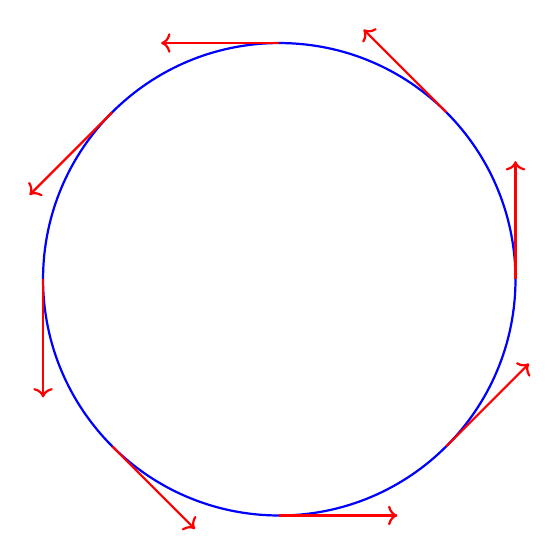
\begin{tikzpicture}[scale=3,thick]
  %circle
  \draw[blue] circle (1cm);

  %arrows
  \draw[red,->] (0:1) -- +(0,0.5);
  \draw[red,->] (45:1) -- +(-0.35,0.35);
  \draw[red,->] (90:1) -- +(-0.5,0);
  \draw[red,->] (135:1) -- +(-0.35,-0.35);
  \draw[red,->] (180:1) -- +(0,-0.5);
  \draw[red,->] (225:1) -- +(0.35,-0.35);
  \draw[red,->] (270:1) -- +(0.5,0);
  \draw[red,->] (315:1) -- +(0.35,0.35);
\end{tikzpicture}
\caption{Orientation for the circle}
\label{fig:orcirc}
\end{figure}
\\
\begin{figure}[h!]
\centering
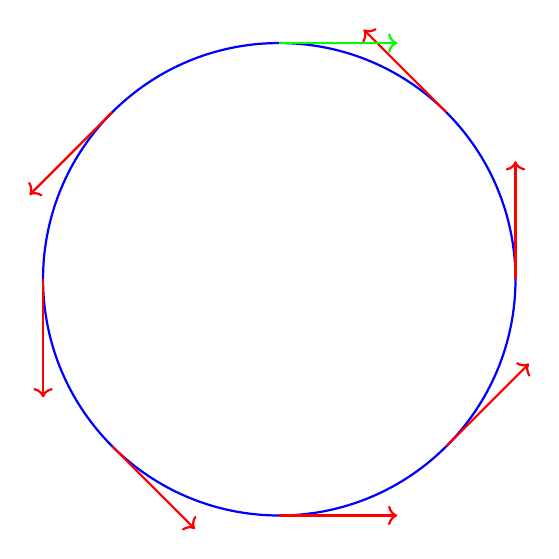
\begin{tikzpicture}[scale=3,thick]
  %circle
  \draw[blue] circle (1cm);

  %arrows
  \draw[red,->] (0:1) -- +(0,0.5);
  \draw[red,->] (45:1) -- +(-0.35,0.35);
  \draw[green,->] (90:1) -- +(0.5,0);
  \draw[red,->] (135:1) -- +(-0.35,-0.35);
  \draw[red,->] (180:1) -- +(0,-0.5);
  \draw[red,->] (225:1) -- +(0.35,-0.35);
  \draw[red,->] (270:1) -- +(0.5,0);
  \draw[red,->] (315:1) -- +(0.35,0.35);
\end{tikzpicture}
\caption{Not an orientation for the circle}
\label{fig:norcirc}
\end{figure}
\\

\item[(b)]
The standard example for a tangentially non-orientable manifold is the open M{\"o}bius strip which can be given by identifying the top and the bottom of the square in the opposite direction, i.e.
\begin{align*}
  (0,1)
  \times
  [0,1]
  \qquad
  \text{with}
  \qquad
  (x_{1},0)
  \sim
  (1-x_{1},1)
  \quad
  \text{for }
  x_{1}
  \in
  (0,1)
\end{align*}
as depicted in figure \ref{fig:moebius}. This means that the square is twisted once before the top and bottom edge are glued together. An orientation would be a consistent choice of a $2$-dimensional basis for the tangent space at each point but the twist basically reverses one direction of this basis without changing the other, thus reversing the whole orientation at the top/bottom edge as illustrated in figure \ref{fig:moebius}.
\\
%/*
%\iffalse
\begin{figure}[h!]
\centering
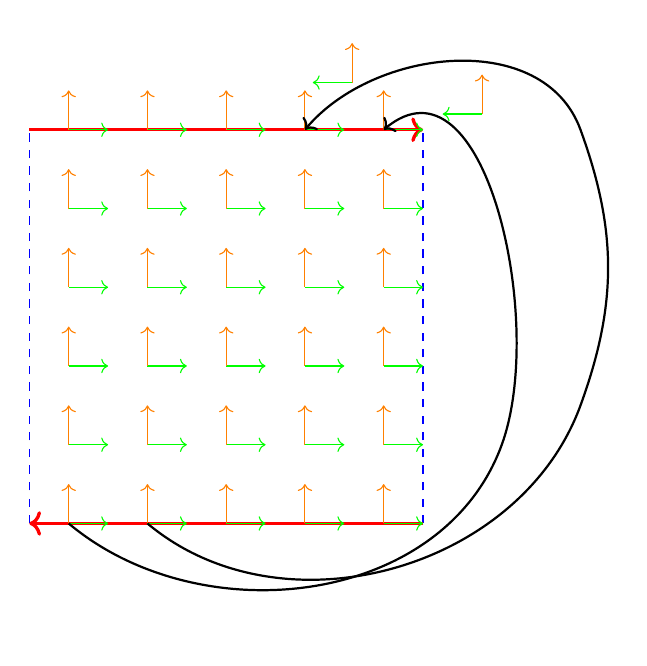
\begin{tikzpicture}[scale=5,thick]
  %rectangle
  \draw[blue,thin,dashed] (0,0) -- (0,1);
  \draw[red,very thick,->] (0,1) -- (1,1);
  \draw[blue,thin,dashed] (1,0) -- (1,1);
  \draw[red,very thick,->] (1,0) -- (0,0);

  %orientations
  %left
  \draw[green,->,thin] (0.1,0) -- +(0.1,0);
  \draw[orange,->,thin] (0.1,0) -- +(0,0.1);
  \draw[green,->,thin] (0.1,0.2) -- +(0.1,0);
  \draw[orange,->,thin] (0.1,0.2) -- +(0,0.1);
  \draw[green,->,thin] (0.1,0.4) -- +(0.1,0);
  \draw[orange,->,thin] (0.1,0.4) -- +(0,0.1);
  \draw[green,->,thin] (0.1,0.6) -- +(0.1,0);
  \draw[orange,->,thin] (0.1,0.6) -- +(0,0.1);
  \draw[green,->,thin] (0.1,0.8) -- +(0.1,0);
  \draw[orange,->,thin] (0.1,0.8) -- +(0,0.1);
  \draw[green,->,thin] (0.1,1) -- +(0.1,0);
  \draw[orange,->,thin] (0.1,1) -- +(0,0.1);
  %left-middle
  \draw[green,->,thin] (0.3,0) -- +(0.1,0);
  \draw[orange,->,thin] (0.3,0) -- +(0,0.1);
  \draw[green,->,thin] (0.3,0.2) -- +(0.1,0);
  \draw[orange,->,thin] (0.3,0.2) -- +(0,0.1);
  \draw[green,->,thin] (0.3,0.4) -- +(0.1,0);
  \draw[orange,->,thin] (0.3,0.4) -- +(0,0.1);
  \draw[green,->,thin] (0.3,0.6) -- +(0.1,0);
  \draw[orange,->,thin] (0.3,0.6) -- +(0,0.1);
  \draw[green,->,thin] (0.3,0.8) -- +(0.1,0);
  \draw[orange,->,thin] (0.3,0.8) -- +(0,0.1);
  \draw[green,->,thin] (0.3,1) -- +(0.1,0);
  \draw[orange,->,thin] (0.3,1) -- +(0,0.1);
  %middle
  \draw[green,->,thin] (0.5,0) -- +(0.1,0);
  \draw[orange,->,thin] (0.5,0) -- +(0,0.1);
  \draw[green,->,thin] (0.5,0.2) -- +(0.1,0);
  \draw[orange,->,thin] (0.5,0.2) -- +(0,0.1);
  \draw[green,->,thin] (0.5,0.4) -- +(0.1,0);
  \draw[orange,->,thin] (0.5,0.4) -- +(0,0.1);
  \draw[green,->,thin] (0.5,0.6) -- +(0.1,0);
  \draw[orange,->,thin] (0.5,0.6) -- +(0,0.1);
  \draw[green,->,thin] (0.5,0.8) -- +(0.1,0);
  \draw[orange,->,thin] (0.5,0.8) -- +(0,0.1);
  \draw[green,->,thin] (0.5,1) -- +(0.1,0);
  \draw[orange,->,thin] (0.5,1) -- +(0,0.1);
  %right-middle
  \draw[green,->,thin] (0.7,0) -- +(0.1,0);
  \draw[orange,->,thin] (0.7,0) -- +(0,0.1);
  \draw[green,->,thin] (0.7,0.2) -- +(0.1,0);
  \draw[orange,->,thin] (0.7,0.2) -- +(0,0.1);
  \draw[green,->,thin] (0.7,0.4) -- +(0.1,0);
  \draw[orange,->,thin] (0.7,0.4) -- +(0,0.1);
  \draw[green,->,thin] (0.7,0.6) -- +(0.1,0);
  \draw[orange,->,thin] (0.7,0.6) -- +(0,0.1);
  \draw[green,->,thin] (0.7,0.8) -- +(0.1,0);
  \draw[orange,->,thin] (0.7,0.8) -- +(0,0.1);
  \draw[green,->,thin] (0.7,1) -- +(0.1,0);
  \draw[orange,->,thin] (0.7,1) -- +(0,0.1);
  %right
  \draw[green,->,thin] (0.9,0) -- +(0.1,0);
  \draw[orange,->,thin] (0.9,0) -- +(0,0.1);
  \draw[green,->,thin] (0.9,0.2) -- +(0.1,0);
  \draw[orange,->,thin] (0.9,0.2) -- +(0,0.1);
  \draw[green,->,thin] (0.9,0.4) -- +(0.1,0);
  \draw[orange,->,thin] (0.9,0.4) -- +(0,0.1);
  \draw[green,->,thin] (0.9,0.6) -- +(0.1,0);
  \draw[orange,->,thin] (0.9,0.6) -- +(0,0.1);
  \draw[green,->,thin] (0.9,0.8) -- +(0.1,0);
  \draw[orange,->,thin] (0.9,0.8) -- +(0,0.1);
  \draw[green,->,thin] (0.9,1) -- +(0.1,0);
  \draw[orange,->,thin] (0.9,1) -- +(0,0.1);

  %identification
  \draw[->] (0.1,0) to [out=-40,in=-110] (1.2,0.2) to [out=70,in=40] (0.9,1);
  \draw[green,->,thin] (1.15,1.04) -- +(-0.1,0);
  \draw[orange,->,thin] (1.15,1.04) -- +(0,0.1);
  \draw[->] (0.3,0) to [out=-40,in=-110] (1.4,0.3) to [out=70,in=-70] (1.4,1) to [out=110,in=50] (0.7,1);
  \draw[green,->,thin] (0.82,1.12) -- +(-0.1,0);
  \draw[orange,->,thin] (0.82,1.12) -- +(0,0.1);
\end{tikzpicture}
\caption{The open M{\"o}bius strip as non-orientable manifold}
\label{fig:moebius}
\end{figure}
%\fi
%*/
\end{enumerate}
\end{exa}
\begin{prf}
The technical details can be filled in as an exercise.
\\
\phantom{proven}
\hfill
$\Box$
\end{prf}
Let now $(U_{1},\varphi_{1}),(U_{2},\varphi_{2})$ be two charts belonging to a subatlas according to a tangential orientation of $M$, let $x \in U_{1} \cap U_{2}$ and let $(v_{1},\ldots,v_{n})$ be an ordered basis of $T_{x}M$. Then
\begin{align*}
  \left(
    T_{x}\varphi_{1}(v_{1})
    ,
    \ldots
    ,
    T_{x}\varphi_{1}(v_{n})
  \right)
  \qquad
  \text{and}
  \qquad
  \left(
    T_{x}\varphi_{2}(v_{1})
    ,
    \ldots
    ,
    T_{x}\varphi_{2}(v_{n})
  \right)
\end{align*}
belong to the same orientation on $\mathbb{R}^{n}$. Since
\begin{align*}
  T_{x}\varphi_{1}
  &=
  T_{\varphi_{2}(x)}(\varphi_{1} \circ \varphi_{2}^{-1})
  \circ
  T_{x}\varphi_{2}
\end{align*}
we can conclude that
\begin{align*}
  T_{\varphi_{2}(x)}
  \left(
    \varphi_{1}
    \circ
    \varphi_{2}^{-1}
  \right)
\end{align*}
is orientation-preserving for all $x \in U_{1} \cap U_{2}$, that is, the determinant of this linear map - which is nothing but the Jacobian determinant of the transition map $\varphi_{1} \circ \varphi_{2}^{-1}$ at $\varphi_{2}(x)$ - is positive for all $x \in U_{1} \cap U_{2}$. We call a $C^{1}$-diffeomorphism $f \colon O_{1} \to O_{2}$ between open subsets of $\mathbb{R}^{n}$ \textbf{differentiably standard orientation-preserving} if the Jacobian determinant of $f$ is positive at each point in $O_{1}$ and \textbf{differentiably standard orientation-reversing} if the Jacobian determinant is negative everywhere. Note that since the Jacobian determinant for such an $f$ is a continuous function from $O_{1}$ to $\mathbb{R} \setminus \lbrace 0 \rbrace$, its sign is constant if $O_{1}$ is connected. Now a differentiable atlas is called \textbf{differentiably oriented} if all transition maps are differentiably standard orientation-preserving. We say that $M$ is \textbf{differentiably orientable} if there exists a differentiably oriented atlas. A \textbf{differentiable orientation} is then a maximal differentiably oriented atlas, which means that this atlas is not properly contained in another differentiably oriented atlas\footnote{this notion of maximality can, of course, be equivalently defined as the union of all corresponding atlases in an equivalence class where two such atlases are equivalent if their union is again such an atlas}. A manifold together with a differentiable orientation is a \textbf{differentiably oriented manifold}.
\\
Of course, a differentiable orientation on an open submanifold is induced by restricting the charts of the differentiable orientation of $M$. This is because the chart obtained by restricting a chart in the maximal differentiably oriented atlas of $M$ to an open subset is again in that atlas. A $C^{1}$-diffeomorphism $f \colon M_{1} \to M_{2}$ between two differentiably oriented manifolds without boundary is defined to be \textbf{differentiably orientation-preserving} if for each chart $(U_{2},\varphi_{2})$ in the differentiable orientation of $M_{2}$ the chart
\begin{align*}
  \left(
    f^{-1}(U_{2})
    ,
    \varphi_{2}
    \circ
    f
  \right)
\end{align*}
is in the differentiable orientation of $M_{1}$.
\\
Note that in the language of the tangent bundle $TM$ a differentiable orientation is a (maximal) atlas of local trivializations such that the transition functions have only values in
\begin{align*}
  GL_{+}(n)
  \subset
  GL(n)
\end{align*}
But this is actually nothing but a reduction of the structure group of the tangent bundle to $GL_{+}(n)$, providing an equivalent definition for orientation.
\\
\begin{exa}
\label{exa:difforstdpr}
As an example consider open submanifolds $M_{1},M_{2}$ of $\mathbb{R}^{n}$ each equipped with a differentiable orientation and a $C^{1}$-diffeomorphism $f \colon M_{1} \to M_{2}$ such that for each of the corresponding connected components $C_{1} \subset M_{1}$ and $f(C_{1}) \subset M_{2}$ either $(C_{1},\mathrm{id}_{C_{1}})$ and $(f(C_{1}),\mathrm{id}_{f(C_{1})})$ belong to the respective differentiable orientations or neither of them does. Then the notion of a differentiably orientation-preserving $C^{1}$-diffeomorphism coincides with the notion of a differentiably standard orientation-preserving $C^{1}$-diffeomorphism.
\end{exa}
\begin{prf}[Sketch]
This is because if the identity chart for a connected component is contained in the differentiable orientation then all charts in that atlas (and their inverses) are transition maps and therefore differentiably standard orientation-preserving on that component. Else all the charts are differentiably standard orientation-reversing on that component. Then the claim follows because if both maps in a composition of $C^{1}$-diffeomorphisms between open subsets of $\mathbb{R}^{n}$ are differentiably standard orientation-preserving or -reversing then the composition is differentiably standard orientation-preserving and if one of them is differentiably standard orientation-preserving and the other is -reversing then the composition is differentiably standard orientation-reversing.
\\
\phantom{proven}
\hfill
$\Box$
\end{prf}
For the, a priori different, notions of tangential and differentiable orientation we have the following
\\
\begin{thm}
\label{thm:equivtangdiff}
A differentiable $n$-manifold without boundary $M$ is tangentially orientable if and only if it is differentiably orientable.
\end{thm}
\begin{prf}
From what was said before it is clear that a tangential orientation yields a differentiably oriented atlas and that the corresponding differentiable orientation is given by adding all charts to the atlas whose differentials are orientation-preserving at all points w.r.t. the given tangential orientation.
\\
Suppose now that we have a differentiable orientation on $M$. Then we can define an orientation of $T_{x}M$ for $x \in M$ by pulling back the standard orientation of $\mathbb{R}^{n}$ via a chart $(U_{1},\varphi_{1})$ around $x$. This means the orientation on $T_{x}M$ is chosen to be the one containing the basis
\begin{align*}
  \left(
    T_{\varphi_{1}(x)}
    \varphi_{1}^{-1}(e_{1})
    ,
    \ldots
    ,
    T_{\varphi_{1}(x)}
    \varphi_{1}^{-1}(e_{n})
  \right)
\end{align*}
where $(e_{1},\ldots,e_{n})$ is the standard basis of $\mathbb{R}^{n}$. With this orientation $T_{\varphi_{1}(x)}\varphi_{1}^{-1}$ and thus, of course, $T_{x}\varphi_{1}$ are orientation-preserving isomorphisms. For the well-definedness we have to check that the orientation does not depend on the chosen chart. Let $(U_{2},\varphi_{2})$ be another chart around $x$. We know that
\begin{align*}
  (e_{1},\ldots,e_{n})
  \qquad
  \text{and}
  \qquad
  \left(
    T_{\varphi_{2}(x)}(\varphi_{1} \circ \varphi_{2}^{-1})(e_{1})
    ,
    \ldots
    ,
    T_{\varphi_{2}(x)}(\varphi_{1} \circ \varphi_{2}^{-1})(e_{n})
  \right)
\end{align*}
belong to the same orientation of $\mathbb{R}^{n}$. Hence, by applying $T_{\varphi_{1}(x)}\varphi_{1}^{-1}$ we see that
\begin{align*}
  \left(
    T_{\varphi_{1}(x)}\varphi_{1}^{-1}(e_{1})
    ,
    \ldots
    ,
    T_{\varphi_{1}(x)}\varphi_{1}^{-1}(e_{n})
  \right)
  \qquad
  \text{and}
  \qquad
  \left(
    T_{\varphi_{2}(x)}\varphi_{2}^{-1}(e_{1})
    ,
    \ldots
    ,
    T_{\varphi_{2}(x)}\varphi_{2}^{-1}(e_{n})
  \right)
\end{align*}
belong to the same orientation of $T_{x}M$. This additionally shows that $T_{x}\varphi_{2}$ is orientation-preserving as well. Thus these induced orientations on the tangential spaces are a tangential orientation with the given maximal oriented atlas.
\\
\phantom{proven}
\hfill
$\Box$
\end{prf}
It is clear that the constructions in the above proof to obtain a differentiable orientation from a tangential orientation and vice versa are inverse to each other, i.e. applying them consecutively in either order yields the original orientation.
\\\\
The definition of orientability in terms of an oriented atlas makes perfect sense even without a differentiable structure, except for the notion of a differentiably standard orientation-preserving transition map as the transition maps are now merely homeomorphisms and not necessarily $C^{1}$-diffeomorphisms anymore. Thus we need a notion of what it means for a homeomorphism between open subsets of $\mathbb{R}^{n}$ to be orientation-preserving. For this purpose we make use of some singular homology and we will use the notation from the homology chapter in the appendix. So the reader who does not know the notions and symbols here should have a look at the appendix first.
\\
Let $f \colon O_{1} \to O_{2}$ a homeomorphism between open subsets of $\mathbb{R}^{n}$ and let $x \in O_{1}$. Then $f$ induces an isomorphism $f_{x}$ in $\mathbf{Top_{2}}$ between the ordered pairs
\begin{align*}
  (O_{1},O_{1} - \lbrace x \rbrace)
  \qquad
  \text{and}
  \qquad
  (O_{2},O_{2} - \lbrace f(x) \rbrace)
\end{align*}
and hence an isomorphism
\begin{align*}
  H_{n}(f_{x})
  \colon
  H_{n}
  \left(
    (O_{1},O_{1} - \lbrace x \rbrace)
  \right)
  &\to
  H_{n}
  \left(
    (O_{2},O_{2} - \lbrace f(x) \rbrace)
  \right)
\end{align*}
of singular homology groups. By excision, (HT3), we obtain an isomorphism
\begin{align*}
  H_{n}
  \left(
    i_{x,O_{1}}^{\mathbb{R}^{n}}
  \right)
  \colon
  H_{n}
  \left(
    (O_{1},O_{1} - \lbrace x \rbrace)
  \right)
  \to
  H_{n}
  \left(
    (\mathbb{R}^{n},\mathbb{R}^{n} - \lbrace x \rbrace)
  \right)
\end{align*}
induced by the inclusion
\begin{align*}
  i_{x,O_{1}}^{\mathbb{R}^{n}}
  \colon
  (O_{1},O_{1} - \lbrace x \rbrace)
  &\to
  (\mathbb{R}^{n},\mathbb{R}^{n} - \lbrace x \rbrace)
\end{align*}
since
\begin{align*}
  \overline{O_{1}^{c}}
  &=
  O_{1}^{c}
  \subset
  \mathbb{R}^{n}
  -
  \lbrace x \rbrace
\end{align*}
and $\mathbb{R}^{n} - \lbrace x \rbrace$ is open because $\mathbb{R}^{n}$ is Hausdorff and thus singleton sets are closed. Moreover, the translation map
\begin{align*}
  \tau_{x}
  \colon
  \mathbb{R}^{n}
  &\to
  \mathbb{R}^{n}
  ,\qquad
  y
  \mapsto
  y + x
\end{align*}
induces an isomorphism
\begin{align*}
  t_{x}
  \colon
  (\mathbb{R}^{n},\mathbb{R}^{n} - \lbrace 0 \rbrace)
  &\to
  (\mathbb{R}^{n},\mathbb{R}^{n} - \lbrace x \rbrace)
\end{align*}
in $\mathbf{Top_{2}}$ and thus $H_{n}(t_{x})$ is an isomorphism. Composition then yields an isomorphism
\begin{align*}
  \iota_{x,O_{1}}
  &:=
  H_{n}(t_{x}^{-1})
  \circ
  H_{n}(i_{x,O_{1}}^{\mathbb{R}^{n}})
  \colon
  H_{n}
  \left(
    (O_{1},O_{1} - \lbrace x \rbrace)
  \right)
  \to
  H_{n}
  \left(
    (\mathbb{R}^{n},\mathbb{R}^{n} - \lbrace 0 \rbrace)
  \right)
\end{align*}
Analogously, we obtain an isomorphism
\begin{align*}
  \iota_{f(x),O_{2}}
  &:=
  H_{n}(t_{f(x)}^{-1})
  \circ
  H_{n}(i_{f(x),O_{2}}^{\mathbb{R}^{n}})
  \colon
  H_{n}
  \left(
    (O_{2},O_{2} - \lbrace f(x) \rbrace)
  \right)
  \to
  H_{n}
  \left(
    (\mathbb{R}^{n},\mathbb{R}^{n} - \lbrace 0 \rbrace)
  \right)
\end{align*}
Using that $\mathbb{R}^{n}$ is contractible and that $\mathbb{R}^{n} - \lbrace 0 \rbrace$ is homotopy equivalent to the $(n-1)$-sphere $S^{n-1}$ it is not hard to see (cf. e.g. \cite{8b5861fc}) with the long exact sequence of homology groups that
\begin{align*}
  H_{n}((\mathbb{R}^{n},\mathbb{R}^{n} - \lbrace 0 \rbrace))
  &\cong
  \mathbb{Z}
\end{align*}
Hence we define $f$ to be \textbf{topologically standard orientation-preserving} if
\begin{align*}
  \iota_{f(x),O_{2}}
  \circ
  H_{n}(f_{x})
  \circ
  \iota_{x,O_{1}}^{-1}
  &=
  \mathrm{id}_{H_{n}((\mathbb{R}^{n},\mathbb{R}^{n} - \lbrace 0 \rbrace))}
\end{align*}
for each $x \in O_{1}$, that is if these maps all fix the two generators of $H_{n}((\mathbb{R}^{n},\mathbb{R}^{n} - \lbrace 0 \rbrace))$. If the generators are interchanged for all $x \in O_{1}$ we call $f$ \textbf{topologically standard orientation-reversing}. It will become clear later that if $O_{1}$ is connected then either all these maps fix the two generators or all these maps interchange the generators. An atlas of an $n$-manifold without boundary $M$ is then called \textbf{topologically oriented} if all transition maps are topologically standard orientation-preserving. We call $M$ \textbf{topologically orientable} if there exists a topologically oriented atlas. A \textbf{topological orientation} is then a maximal topologically oriented atlas and a manifold together with a topological orientation is a \textbf{topologically oriented manifold}.
\\
Note that for an open subset $\tilde{O}_{1} \subset O_{1}$ with $x \in \tilde{O}_{1}$ the inclusion
\begin{align*}
  i_{x,\tilde{O}_{1}}^{O_{1}}
  \colon
  (\tilde{O}_{1},\tilde{O}_{1} - \lbrace x \rbrace)
  &\to
  (O_{1},O_{1} - \lbrace x \rbrace)
\end{align*}
induces an isomorphism $H_{n}(i_{x,\tilde{O}_{1}}^{O_{1}})$ by excision, (HT3), because $O_{1} - \tilde{O}_{1}$ is closed in $O_{1}$. Analogously, we have an isomorphism induced by $i_{f(x),\tilde{O}_{2}}^{O_{2}}$ for $\tilde{O}_{2} := f(\tilde{O}_{1})$. Further note that
\begin{align*}
  i_{x,O_{1}}^{\mathbb{R}^{n}}
  \circ
  i_{x,\tilde{O}_{1}}^{O_{1}}
  &=
  i_{x,\tilde{O}_{1}}^{\mathbb{R}^{n}}
  \\
  i_{f(x),O_{2}}^{\mathbb{R}^{n}}
  \circ
  i_{f(x),\tilde{O}_{2}}^{O_{2}}
  &=
  i_{f(x),\tilde{O}_{2}}^{\mathbb{R}^{n}}
  \\
  f_{x}
  \circ
  i_{x,\tilde{O}_{1}}^{O_{1}}
  &=
  i_{f(x),\tilde{O}_{2}}^{O_{2}}
  \circ
  \tilde{f_{x}}
\end{align*}
where
\begin{align*}
  \tilde{f_{x}}
  &:=
  f_{x}
  \vert
  (\tilde{O}_{1},\tilde{O}_{1} - \lbrace x \rbrace)
\end{align*}
Applying $H_{n}$ to these equations and using the functoriality we obtain
\begin{align*}
  H_{n}(i_{x,O_{1}}^{\mathbb{R}^{n}})
  \circ
  H_{n}(i_{x,\tilde{O}_{1}}^{O_{1}})
  &=
  H_{n}(i_{x,\tilde{O}_{1}}^{\mathbb{R}^{n}})
  \\
  H_{n}(i_{f(x),O_{2}}^{\mathbb{R}^{n}})
  \circ
  H_{n}(i_{f(x),\tilde{O}_{2}}^{O_{2}})
  &=
  H_{n}(i_{f(x),\tilde{O}_{2}}^{\mathbb{R}^{n}})
  \\
  H_{n}(f_{x})
  \circ
  H_{n}(i_{x,\tilde{O}_{1}}^{O_{1}})
  &=
  H_{n}(i_{f(x),\tilde{O}_{2}}^{O_{2}})
  \circ
  H_{n}(\tilde{f_{x}})
\end{align*}
With these equations it is easy to see that
\begin{align*}
  \iota_{f(x),\tilde{O}_{2}}
  \circ
  H_{n}(\tilde{f_{x}})
  \circ
  \iota_{x,\tilde{O}_{1}}^{-1}
  &=
  \iota_{f(x),O_{2}}
  \circ
  H_{n}(f_{x})
  \circ
  \iota_{x,O_{1}}^{-1}
\end{align*}
which shows that restrictions of topologically standard orientation-preserving homeomorphisms to open subsets are again topologically standard orientation-preserving. It further shows that it suffices to find a topologically standard orientation-preserving restriction to an open neighbourhood for any point in $O_{1}$ to show that $f$ is topologically standard orientation-preserving. As any open set of $\mathbb{R}^{n}$, and more generally any manifold, is locally path-connected we know that any connected component is open. Thus it suffices in particular to show that $f$ is topologically standard orientation-preserving on each component.
\\
From this it is immediate that restrictions of charts of a topological orientation to open subsets are also in that topological orientation. Therefore we obtain a topological orientation on an open submanifold by restriction. Moreover, a homeomorphism $f \colon M_{1} \to M_{2}$ between two topologically oriented manifolds without boundary is \textbf{topologically orientation-preserving} if for each chart $(U_{2},\varphi_{2})$ in the topological orientation of $M_{2}$ the chart
\begin{align*}
  \left(
    f^{-1}(U_{2})
    ,
    \varphi_{2}
    \circ
    f
  \right)
\end{align*}
is in the topological orientation of $M_{1}$. In the case of two open submanifolds of $\mathbb{R}^{n}$ this notion coincides with the notion of a topologically standard orientation-preserving homeomorphism under the same conditions as in the differentiable case and also the reasoning is the same.
\\\\
There is another way to define an orientation for an $n$-manifold without boundary $M$ in terms of singular homology. Consider the singular homology group $H_{n}((M,M - \lbrace x \rbrace))$ for $x \in M$, which we call the \textbf{local homology group (of $M$ at $x$)}. As $M$ is Hausdorff, (HT3) yields an isomorphism
\begin{align*}
  H_{n}(i_{x,U}^{M})
  \colon
  H_{n}((U,U - \lbrace x \rbrace))
  &\to
  H_{n}((M,M - \lbrace x \rbrace))
\end{align*}
induced by the inclusion
\begin{align*}
  i_{x,U}^{M}
  \colon
  (U,U - \lbrace x \rbrace)
  \to
  (M,M - \lbrace x \rbrace)
\end{align*}
for any open neighbourhood $U \subset M$ of $x$. By taking a chart $\varphi \colon U \to O$ we obtain an isomorphism
\begin{align*}
  H_{n}(\varphi_{x})
  \colon
  H_{n}((U,U - \lbrace x \rbrace))
  &\to
  H_{n}((O,O - \lbrace \varphi(x) \rbrace))
\end{align*}
induced by
\begin{align*}
  \varphi_{x}
  \colon
  (U,U - \lbrace x \rbrace)
  &\to
  (O,O - \lbrace \varphi(x) \rbrace)
\end{align*}
which is induced by $\varphi$. Hence, we can conclude from what we know about open subsets of $\mathbb{R}^{n}$ that $H_{n}((M,M - \lbrace x \rbrace))$ is isomorphic to $\mathbb{Z}$. We say that a generator
\begin{align*}
  \mu_{x}^{M}
  \in
  H_{n}((M,M - \lbrace x \rbrace))
\end{align*}
is a \textbf{local orientation (of $M$ at $x$)}. Let
\begin{align*}
  j_{x,U}^{M}
  \colon
  (M,M - U)
  &\to
  (M,M - \lbrace x \rbrace)
\end{align*}
denote the inclusion for $x \in U \subset M$. For $U$ open we call an element
\begin{align*}
  \mu_{U}^{M}
  \in
  H_{n}((M,M - U))
\end{align*}
such that $H_{n}(j_{y,U}^{M})(\mu_{U}^{M})$ is a generator of $H_{n}((M,M - \lbrace y \rbrace))$ for all $y \in U$ a \textbf{local orientation (of $M$) along $U$}. Note that if
\begin{align*}
  j_{V,U}^{M}
  \colon
  (M,M - U)
  &\to
  (M,M - V)
\end{align*}
denotes the inclusion for open $V \subset U$ then we have
\begin{align}
\label{funcincl}
  H_{n}(j_{y,V}^{M})
  \left(
    H_{n}(j_{V,U}^{M})(\mu_{U}^{M})
  \right)
  &=
  H_{n}(j_{y,U}^{M})(\mu_{U}^{M})
\end{align}
for any $y \in V$ since $H_{n}$ is a functor and
\begin{align*}
  j_{y,V}^{M}
  \circ
  j_{V,U}^{M}
  &=
  j_{y,U}^{M}
\end{align*}
Thus $H_{n}(j_{V,U}^{M})(\mu_{U}^{M})$ is a local orientation along $V$. Now a \textbf{homological orientation} of $M$ is a \textbf{continuous\footnote{the reason for this terminology is that this can also be expressed to be a continuous section of a certain bundle, the so called orientation bundle (see e.g. \cite{ad05eef9})} choice} of local orientations $\mu_{x}^{M}$ at each $x \in M$ where continuous means that for every $x \in M$ there is an open neighbourhood $U$ of $x$ and a local orientation $\mu_{U}^{M}$ along $U$ such that
\begin{align*}
  H_{n}(j_{y,U}^{M})(\mu_{U}^{M})
  &=
  \mu_{y}^{M}
  \qquad
  \text{for all }
  y
  \in
  U
\end{align*}
We call $M$ \textbf{homologically orientable} if such a homological orientation exists and such a manifold together with a homological orientation is a \textbf{homologically oriented manifold}. As $M$ is locally Euclidean there is a neighbourhood $V \subset U$ of $x$ that is homeomorphic to an open subset of $\mathbb{R}^{n}$ and we can choose an open subset $B \subset V$ with $x \in B$ which is homeomorphic to an open ball of finite radius in $\mathbb{R}^{n}$ such that $\overline{B} \subset V$. One then easily verifies (cf. e.g. \cite{1a21f4c7}) that $H_{n}(j_{y,B}^{M})$ is an isomorphism for all $y \in B$. From \eqref{funcincl} we can hence conclude that
\begin{align*}
  \mu_{B}^{M}
  &:=
  H_{n}(j_{B,U}^{M})(\mu_{U}^{M})
\end{align*}
is a generator of $H_{n}((M,M - B))$ which is mapped to $\mu_{y}^{M}$ by $H_{n}(j_{y,B}^{M})$ for all $y \in B$ and hence that we could equivalently demand the existence of such $V$, $B$ and $\mu_{B}^{M}$ instead of $\mu_{U}^{M}$ for the continuous choice of local orientations.
\\
For orientations on open submanifolds we have the following
\\
\begin{lem}
\label{lem:homorsub}
Given a homologically oriented manifold $M$. For an open submanifold $U \subset M$ the homological orientation on $M$ induces a homological orientation on $U$ by the inverse of the isomorphism $H_{n}(i_{x,U}^{M})$ for each $x \in U$, i.e. the local orientations are
\begin{align*}
  \mu_{x}^{U}
  &:=
  H_{n}(i_{x,U}^{M})^{-1}(\mu_{x}^{M})
  \in
  H_{n}((U,U - \lbrace x \rbrace))
\end{align*}
\end{lem}
\begin{prf}
We have to show that this choice is indeed continuous. To this end let $x \in U$ and let $V$, $B$ and $\mu_{B}^{M}$ as for the continuous choice for $M$, where we can choose them such that $V \subset U$. By (HT3) the map
\begin{align*}
  H_{n}(i_{B,U}^{M})
  \colon
  H_{n}((U,U - B))
  &\to
  H_{n}((M,M - B))
\end{align*}
induced by the inclusion
\begin{align*}
  i_{B,U}^{M}
  \colon
  (U,U - B)
  &\to
  (M,M - B)
\end{align*}
is an isomorphism since $\overline{B} \subset U$ and hence
\begin{align*}
  U^{c}
  \subset
  M
  -
  \overline{B}
  &=
  \mathring{(M - B)}
\end{align*}
Let now
\begin{align*}
  \mu_{B}^{U}
  &:=
  H_{n}(i_{B,U}^{M})^{-1}
  \left(
    \mu_{B}^{M}
  \right)
  \in
  H_{n}((U,U - B))
\end{align*}
Note that the following diagram commutes
\begin{equation*}
\begin{tikzcd}[row sep=4em,column sep=3em]
  (U,U - B)
  \ar{r}{i_{B,U}^{M}}
  \ar{d}[swap]{j_{y,B}^{U}}
  &
  (M,M - B)
  \ar{d}{j_{y,B}^{M}}
  \\
  (U,U - \lbrace y \rbrace)
  \ar{r}{i_{y,U}^{M}}
  &
  (M,M - \lbrace y \rbrace)
\end{tikzcd}
\end{equation*}
and the functoriality of $H_{n}$ thus implies
\begin{align}
\label{inclcomm}
  H_{n}(i_{y,U}^{M})
  \circ
  H_{n}(j_{y,B}^{U})
  &=
  H_{n}(j_{y,B}^{M})
  \circ
  H_{n}(i_{B,U}^{M})
\end{align}
for all $y \in B$. Hence we find
\begin{align*}
  H_{n}(j_{y,B}^{U})(\mu_{B}^{U})
  &=
  H_{n}(j_{y,B}^{U})
  \left(
    H_{n}(i_{B,U}^{M})^{-1}(\mu_{B}^{M})
  \right)
  \\
  &=
  H_{n}(i_{y,U}^{M})^{-1}
  \left(
    H_{n}(j_{y,B}^{M})(\mu_{B}^{M})
  \right)
  \\
  &=
  H_{n}(i_{y,U}^{M})^{-1}(\mu_{y}^{M})
  \\
  &=
  \mu_{y}^{U}
\end{align*}
for all $y \in B$ showing that our choice is indeed continuous.
\\
\phantom{proven}
\hfill
$\Box$
\end{prf}
\begin{exa}
\label{exa:homorrn}
We now want to endow $\mathbb{R}^{n}$ with a homological orientation, but we will gloss over some details here as this involves some direct dealing with singular simplices. One can show that one of the generators
\begin{align*}
  \mu_{0}^{\mathbb{R}^{n}}
  \in
  H_{n}((\mathbb{R}^{n},\mathbb{R}^{n} - \lbrace 0 \rbrace))
\end{align*}
can be represented by mapping the $n$-dimensional standard simplex to the $n$-dimensional simplex spanned by
\begin{align*}
  \left(
    -
    \sum_{i = 1}^{n}
    e_{i}
    ,
    e_{1}
    ,
    \ldots
    ,
    e_{n}
  \right)
\end{align*}
where $(e_{1},\ldots,e_{n})$ is the standard basis of $\mathbb{R}^{n}$. One can further show that by scaling the image of this singular simplex by some factor or translating it one still obtains a representative of $\mu_{0}^{\mathbb{R}^{n}}$ as long as $0$ is in its interior. We define the local orientation $\mu_{x}^{\mathbb{R}^{n}}$ at each point $x \in \mathbb{R}^{n}$ by using the isomorphism $H_{n}(t_{x})$, i.e.
\begin{align*}
  \mu_{x}^{\mathbb{R}^{n}}
  &=
  H_{n}(t_{x})(\mu_{0}^{\mathbb{R}^{n}})
\end{align*}
This means we basically translate the image of the singular simplex from above in such a way that $x$ is in its interior. To see that this is a homological orientation let $\mathbb{B}$ be a ball of finite radius around $x$ that is contained in the interior of the image of the representative of $\mu_{x}^{\mathbb{R}^{n}}$ and let
\begin{align*}
  \mu_{\mathbb{B}}^{\mathbb{R}^{n}}
  \in
  H_{n}(\mathbb{R}^{n},\mathbb{R}^{n} - \mathbb{B})
\end{align*}
be the generator that is mapped to $\mu_{x}^{\mathbb{R}^{n}}$ by $H_{n}(j_{x,\mathbb{B}}^{\mathbb{R}^{n}})$. $\mu_{\mathbb{B}}^{\mathbb{R}^{n}}$ can be represented by the same map as $\mu_{x}^{\mathbb{R}^{n}}$ and moreover this map is a representative of $\mu_{y}^{\mathbb{R}^{n}}$ for all $y \in \mathbb{B}$ which implies that
\begin{align*}
  H_{n}(j_{y,\mathbb{B}}^{\mathbb{R}^{n}})
  \left
    (\mu_{\mathbb{B}}^{\mathbb{R}^{n}}
  \right)
  &=
  \mu_{y}^{\mathbb{R}^{n}}
\end{align*}
This shows that the choice we made is continuous.
\end{exa}
\begin{prf}
The technical details can be filled in by the reader with sufficient knowledge about singular homology.
\\
\phantom{proven}
\hfill
$\Box$
\end{prf}
From the above we have a homological orientation for every open subset of $\mathbb{R}^{n}$ determined by a fixed generator of $H_{n}((\mathbb{R}^{n},\mathbb{R}^{n} - \lbrace 0 \rbrace))$ and from now on we will always assume that the same generator is used whenever we consider an open subset of $\mathbb{R}^{n}$ as a homologically oriented manifold.
\\
We say that a homeomorphism $f \colon M_{1} \to M_{2}$ between homologically oriented $n$-manifolds without boundary \textbf{preserves the local orientation (at $x \in M_{1}$)} if the map induced on the local homology groups maps the local orientation at $x$ of the given orientation on $M_{1}$ to the local orientation at $f(x)$ of the given orientation on $M_{2}$. Otherwise we say that $f$ \textbf{reverses the local orientation (at $x \in M$)}. $f$ is called \textbf{homologically orientation-preserving} if it preserves all local orientations. Note that in the case of two open subsets of $\mathbb{R}^{n}$ this coincides with the notion of a topologically standard orientation-preserving map with the homological orientation from example \ref{exa:homorrn}.
\\\\
For the two notions of topological and homological orientation we have the following
\\
\begin{thm}
\label{thm:equivtophom}
An $n$-manifold without boundary $M$ is topologically orientable if and only if it is homologically orientable.
\end{thm}
\begin{prf}
\begin{enumerate}
\item[i)]
Given a homological orientation on $M$ we obtain an atlas by taking all charts that are homologically orientation-preserving with respect to the induced homological orientations on the subsets. To see this let $x \in M$ and let $U$, $B$ and $\mu_{B}^{M}$ as in the condition for a continuous choice of local orientations such that there is a chart $\varphi \colon U \to O$, which is possible for every $x \in M$. Let further
\begin{align*}
  \mu_{B}^{U}
  &:=
  H_{n}(i_{B,U}^{M})^{-1}(\mu_{B}^{M})
\end{align*}
We know that $H_{n}(j_{y,B}^{U})$ is an isomorphism and that\footnote{see the proof of lemma \ref{lem:homorsub}}
\begin{align*}
  H_{n}(j_{y,B}^{U})(\mu_{B}^{U})
  &=
  \mu_{y}^{U}
\end{align*}
for all $y \in B$, where $\mu_{y}^{U}$ is the local orientation of $H_{n}((U,U - \lbrace y \rbrace))$ in the induced homological orientation on $U$. Let $\mathbb{B} := \varphi(B)$, then by shrinking $B$ around $x$ if necessary we can assume that $H_{n}(j_{\varphi(y),\mathbb{B}}^{O})$ is an isomorphism and that we have a generator
\begin{align*}
  \mu_{\mathbb{B}}^{O} \in H_{n}((O,O - \mathbb{B}))
\end{align*}
such that
\begin{align*}
  H_{n}(j_{\varphi(y),\mathbb{B}}^{O})
  \left(
    \mu_{\mathbb{B}}^{O}
  \right)
  &=
  \mu_{\varphi(y)}^{O}
\end{align*}
for all $y \in B$, where $\mu_{\varphi(y)}^{O}$ is the local orientation of $H_{n}((O,O - \lbrace \varphi(y) \rbrace))$ in the homological orientation of $O$. The homeomorphism $\varphi$ induces an isomorphism
\begin{align*}
  \varphi_{B}
  \colon
  (U,U - B)
  &\to
  (O,O - \mathbb{B})
\end{align*}
which in turn induces an isomorphism
\begin{align*}
  H_{n}(\varphi_{B})
  \colon
  H_{n}((U,U - B))
  &\to
  H_{n}((O,O - \mathbb{B}))
\end{align*}
that must map (the generator) $\mu_{B}^{U}$ to one of the two generators of $H_{n}(O,O - \mathbb{B})$. By composing $\varphi$ with a reflection of $\mathbb{R}^{n}$ if necessary we can assume\footnote{this is shown e.g. in \cite{8b5861fc}} that
\begin{align*}
  H_{n}(\varphi_{B})(\mu_{B}^{U})
  &=
  \mu_{\mathbb{B}}^{O}
\end{align*}
Now since
\begin{equation*}
\begin{tikzcd}[row sep=4em,column sep=3em]
  (U,U - B)
  \ar{r}{\varphi_{B}}
  \ar{d}[swap]{j_{y,B}^{U}}
  &
  (O,O - \mathbb{B})
  \ar{d}{j_{\varphi(y),\mathbb{B}}^{O}}
  \\
  (U,U - \lbrace y \rbrace)
  \ar{r}{\varphi_{y}}
  &
  (O,O - \lbrace \varphi(y) \rbrace)
\end{tikzcd}
\end{equation*}
commutes, the functoriality of $H_{n}$ implies
\begin{align}
\label{chartcomm}
  H_{n}(\varphi_{y})
  \circ
  H_{n}(j_{y,B}^{U})
  &=
  H_{n}(j_{\varphi(y),\mathbb{B}}^{O})
  \circ
  H_{n}(\varphi_{B})
\end{align}
for all $y \in B$. Hence we find that
\begin{align*}
  H_{n}(\varphi_{y})(\mu_{y}^{U})
  &=
  \mu_{\varphi(y)}^{O}
\end{align*}
for all $y \in B$, which implies
\begin{align*}
  H_{n}
  \left(
    \varphi_{y}\vert(B,B - \lbrace y \rbrace)
  \right)
  \left(
    \mu_{y}^{B}
  \right)
  &=
  \mu_{\varphi(y)}^{\mathbb{B}}
\end{align*}
for the induced\footnote{of course, it does not matter whether they are induced from $M$ or $U$ ($\mathbb{R}^{n}$ or $O$) since $\mu_{y}^{B} = H_{n}(i_{y,B}^{U})^{-1}(\mu_{y}^{U}) = H_{n}(i_{y,B}^{M})^{-1}(\mu_{y}^{M})$ because $i_{y,B}^{M} = i_{y,U}^{M} \circ i_{y,B}^{U}$ and $\mu_{y}^{U} = H_{n}(i_{y,U}^{M})^{-1}(\mu_{y}^{M})$} orientations because
\begin{equation*}
\begin{tikzcd}[row sep=4em,column sep=5em]
  (B,B - \lbrace y \rbrace)
  \ar{r}{\varphi_{y}\vert(B,B - \lbrace y \rbrace)}
  \ar{d}[swap]{i_{y,B}^{U}}
  &
  (\mathbb{B},\mathbb{B} - \lbrace \varphi(y) \rbrace)
  \ar{d}{i_{\varphi(y),\mathbb{B}}^{O}}
  \\
  (U,U - \lbrace y \rbrace)
  \ar{r}{\varphi_{y}}
  &
  (O,O - \lbrace y \rbrace)
\end{tikzcd}
\end{equation*}
commutes. This shows that the chart $(B,\varphi\vert B)$ around $x$ is homologically orientation-preserving so that these charts indeed form an atlas.
\\
Moreover, the last argument shows that the restriction of a homologically orientation-preserving chart to an open subset is again homologically orientation-preserving and also that if such a restriction is homologically orientation-preserving then the local orientations for the points in the domain of the restriction are preserved by the original map. This means it suffices to have a homologically orientation-preserving restriction to an open subset for every point to show that the original map is homologically orientation-preserving\footnote{in particular it suffices to consider restrictions to connected components}. Therefore all transition maps of the considered atlas are homologically and thus topologically standard orientation-preserving so that we have a topologically oriented atlas. It is rather immediate that this atlas is actually maximal. For if $(U,\varphi)$ is a chart such that all transition maps with charts from this atlas are topologically standard orientation-preserving then for each chart $(V,\psi)$ of the considered atlas the restriction of $\varphi$ to $U \cap V$ is homologically orientation-preserving as $\psi$ is homologically orientation-preserving. Since the charts of the atlas cover the whole manifold this shows that $\varphi$ is homologically orientation-preserving on $U$, i.e. $(U,\varphi)$ belongs to the atlas and we have indeed a topological orientation.

\item[ii)]
Conversely, if we have a topological orientation we use the charts of that atlas to transfer the local orientations of the open subsets of $\mathbb{R}^{n}$ to local orientations of $M$: for a chart $\varphi \colon U \to O$ we have the induced isomorphism
\begin{align*}
  H_{n}(\varphi_{x})^{-1}
  \colon
  H_{n}((O,O - \lbrace \varphi(x) \rbrace))
  &\to
  H_{n}((U,U - \lbrace x \rbrace))
\end{align*}
for $x \in U$. Then the isomorphism $H_{n}(i_{x,U}^{M})$ yields a local orientation of $H_{n}((M,M - \lbrace x \rbrace))$,
\begin{align*}
  \mu_{x}^{M}
  &:=
  H_{n}(i_{x,U}^{M})
  \left(
    H_{n}(\varphi_{x})^{-1}
    \left(
      \mu_{\varphi(x)}^{O}
    \right)
  \right)
\end{align*}
With these local orientations $\varphi$ is homologically orientation-preserving. As the atlas is topologically oriented this local orientation does not depend on the chosen chart. More precisely, note that the restriction $(W,\varphi\vert W)$ of a chart from the atlas with $W \subset U$ open induces the same local orientations on $M$ as the original chart since with $Q := \varphi(W)$ we have
\begin{align*}
  &
  \left(
    H_{n}(i_{y,W}^{M})
    \circ
    H_{n}
    \left(
       \varphi_{y}\vert(W,W - \lbrace y \rbrace)
    \right)^{-1}
  \right)
  (\mu_{\varphi(y)}^{Q})
  \\
  &=
  \left(
    H_{n}(i_{y,W}^{M})
    \circ
    H_{n}
    \left(
       i_{y,W}^{U}
    \right)^{-1}
    \circ
    H_{n}
    \left(
       \varphi_{y}
    \right)^{-1}
    \circ
    H_{n}
    \left(
       i_{\varphi(y),Q}^{O}
    \right)
  \right)
  \left(
    H_{n}
    \left(
       i_{\varphi(y),Q}^{\mathbb{R}^{n}}
    \right)^{-1}
    (\mu_{\varphi(y)}^{\mathbb{R}^{n}})
  \right)
  \\
  &=
  \left(
    H_{n}(i_{y,U}^{M})
    \circ
    H_{n}
    \left(
       \varphi_{y}
    \right)^{-1}
  \right)
  \left(
    H_{n}
    \left(
       i_{\varphi(y),O}^{\mathbb{R}^{n}}
    \right)^{-1}
    (\mu_{\varphi(y)}^{\mathbb{R}^{n}})
  \right)
  \\
  &=
  \left(
    H_{n}(i_{y,U}^{M})
    \circ
    H_{n}
    \left(
       \varphi_{y}
    \right)^{-1}
  \right)
  (\mu_{\varphi(y)}^{O})
\end{align*}
for $y \in W$. Let now $(V,\psi)$ be another chart from the topological orientation. As all transition maps are topologically standard orientation-preserving we can conclude that $\psi\vert(V \cap U)$ is homologically orientation-preserving with the local orientations induced by $\varphi$, hence in particular induces the same local orientation of $M$ at $x$ as $\varphi$. But then the latter is also true for $\psi$ itself which follows from the above argument.
\\
To show that this choice of local orientations is indeed continuous, we use that the choice of local orientations of $O$ is continuous, i.e. for each $x \in U$ there is an open neighbourhood $\mathbb{B} \subset O$ of $\varphi(x)$ and an element
\begin{align*}
  \mu_{\mathbb{B}}^{O}
  \in
  H_{n}((O,O - \mathbb{B}))
\end{align*}
such that
\begin{align*}
  H_{n}(j_{\varphi(y),\mathbb{B}}^{O})
  \left(
    \mu_{\mathbb{B}}^{O}
  \right)
  &=
  \mu_{\varphi(y)}^{O}
\end{align*}
for all
\begin{align*}
  y
  \in
  \varphi^{-1}(\mathbb{B})
  =:
  B
\end{align*}
where $\mu_{\varphi(y)}^{O}$ is the local orientation of $H_{n}((O,O - \lbrace \varphi(y) \rbrace))$. For the induced local orientation of $H_{n}((U,U - \lbrace y \rbrace))$,
\begin{align*}
  \mu_{y}^{U}
  &=
  H_{n}(i_{y,U}^{M})^{-1}
  \left(
    \mu_{y}^{M}
  \right)
  \\
  &=
  H_{n}(\varphi_{y})^{-1}
  \left(
    \mu_{\varphi(y)}^{O}
  \right)
\end{align*}
we can conclude from \eqref{chartcomm} that with
\begin{align*}
  \mu_{B}^{U}
  &:=
  H_{n}(\varphi_{B})^{-1}
  \left(
    \mu_{\mathbb{B}}^{O}
  \right)
\end{align*}
we have
\begin{align*}
  H_{n}(j_{y,B}^{U})(\mu_{B}^{U})
  &=
  \mu_{y}^{U}
\end{align*}
for all $y \in B$. We can choose $\mathbb{B}$ such that $\overline{\mathbb{B}} \subset O$ and thus $\overline{B} \subset U$. Hence by (HT3) the map
\begin{align*}
  H_{n}(i_{B,U}^{M})
  \colon
  H_{n}((U,U - B))
  &\to
  H_{n}((M,M - B))
\end{align*}
is an isomorphism. Therefore we can conclude from \eqref{inclcomm} that
\begin{align*}
  \mu_{B}^{M}
  &:=
  H_{n}(i_{B,U}^{M})(\mu_{B}^{U})
  \in
  H_{n}((M,M - B))
\end{align*}
is a local orientation along $B$ with
\begin{align*}
  H_{n}(j_{y,B}^{M})(\mu_{B}^{M})
  &=
  \mu_{y}^{M}
\end{align*}
for all $y \in B$.
\end{enumerate}
\phantom{proven}
\hfill
$\Box$
\end{prf}
It is again clear that the constructions in the above proof to obtain a homological orientation from a topological orientation and vice versa are inverse to each other.
\\\\
Now we have two equivalent definitions of orientation for topological manifolds without boundary and three more that are equivalent to each other for the differentiable case. Of course, we also want to show that all of them are equivalent in the differentiable case, which is why we shortly sketch now that the notion of topological orientation is equivalent to the notion of differentiable orientation. In order to do this we basically only need that the two senses of what it means for a transition map to be standard orientation-preserving coincide if $M$ has a differentiable structure. Then a differentiable orientation gives a topologically oriented atlas and we obtain a topological orientation by taking the corresponding maximal topologically oriented atlas. The other way around, if we have a topological orientation we can take the differentiable charts of this atlas to obtain a differentiable orientation. The two processes are clearly mutually inverse. Thus, what we need is
\\
\begin{lem}
\label{lem:stdorpr}
For a diffeomorphism $f \colon O_{1} \to O_{2}$ between two open subsets of $\mathbb{R}^{n}$ the Jacobian determinant is positive for each $x \in O_{1}$ if and only if $f$ preserves all local orientations.
\end{lem}
\begin{prf}[Sketch]
As both properties only depend on a ball of finite radius around $x$ which is contained in $O_{1}$ we may assume that $O_{1}$ is such a ball. Moreover, since pre- and post-composing with translations does not change anything here, we may assume that $x = f(x) = 0$. For this case the equivalence of the properties is basically given in \cite{ad05eef9}. 
\\
\phantom{proven}
\hfill
$\Box$
\end{prf}
Altogether we have shown that all the definitions we gave for orientation are equivalent, if they can be made. So we will usually drop the adjectives we used to distinguish them and simply speak of an orientation from now on. We can form categories with objects the oriented $C^{r}$-manifolds and morphisms the orientation-preserving $C^{r}$-diffeomorphisms between them, called $\mathbf{DiffOr}_{r}$ (these categories are groupoids, of course). Note that the empty manifold is again an object of any of these categories, but apart from the identity morphism, given by the unique empty map, there is no morphism for this object.
\\\\
An easy but important property concerning orientation is the following
\\
\begin{thm}
\label{thm:connifftwoor}
Let $M$ be an orientable topological $n$-manifold without boundary. Then $M$ is connected if and only if $M$ has exactly two orientations.
\end{thm}
\begin{prf}
\begin{enumerate}
\item[(i)]
Suppose first that $M$ is connected and that we are given two orientations of $M$. Let $A \subset M$ be the subset of all points $x$ for which the local orientations $\mu_{x}^{M}$ and $\tilde{\mu}_{x}^{M}$ of the two given orientations coincide and thus $A^{c}$ the subset on which they disagree. For each $x \in A$ there is an open neighbourhood $B \subset M$ of $x$ and a generator
\begin{align*}
  \mu_{B}^{M}
  \in
  H_{n}((M,M - B))
\end{align*}
such that
\begin{align*}
  H_{n}(j_{y,B}^{M})(\mu_{B}^{M})
  &=
  \mu_{y}^{M}
\end{align*}
for all $y \in B$. By shrinking $B$ if neccessary we may assume that there is a generator
\begin{align*}
\tilde{\mu}_{B}^{M} \in H_{n}((M,M - B))
\end{align*}
such that
\begin{align*}
  H_{n}(j_{y,B}^{M})(\tilde{\mu}_{B}^{M})
  &=
  \tilde{\mu}_{y}^{M}
\end{align*}
for all $y \in B$. As $x \in A$ we know that
\begin{align*}
  H_{n}(j_{x,B}^{M})(\mu_{B}^{M})
  &=
  \mu_{x}^{M}
  \\
  &=
  \tilde{\mu}_{x}^{M}
  \\
  &=
  H_{n}(j_{y,B}^{M})(\tilde{\mu}_{B}^{M})
\end{align*}
and hence we can conclude that
\begin{align*}
  \tilde{\mu}_{B}^{M}
  &=
  \mu_{B}^{M}
\end{align*}
as $H_{n}(j_{x,B}^{M})$ is an isomorphism. This implies
\begin{align*}
  \tilde{\mu}_{y}^{M}
  &=
  H_{n}(j_{y,B}^{M})(\mu_{B}^{M})
  =
  \mu_{y}^{M}
\end{align*}
for all $y \in B$ which means that $B \subset A$ and shows that $A$ is open in $M$. In the same fashion it follows that $A^{c}$ is open in $M$ and thus, since $M$ is connected, that either $A = \emptyset$ or $A = M$, i.e. either all local orientations agree and the two orientations are the same or none of the local orientations agree. As there are exactly two local orientations for each point this shows that there are exactly two orientations for connected $M$. This is because there is at least one orientation since $M$ is orientable and reversing all local orientations clearly yields another one as we can also reverse the local orientations along open sets homeomorphic to open balls.

\item[(ii)]
Now if $M$ is not connected then there are at least two connected components. Thus given an orientation of $M$ we can choose one component and take the opposite local orientations for all points in that component. As the continuity condition for the choice of local orientations only depends on an open neighbourhood for each point and since we can always choose this neighbourhood to be contained in the connected component\footnote{as these are open for manifolds} of the considered point, we obtain another orientation of $M$. But this orientation is clearly different from the original orientation and also from the orientation obtained by reversing all local orientations, hence we have more than two orientations.
\end{enumerate}
\phantom{proven}
\hfill
$\Box$
\end{prf}
The orientation obtained by taking the opposite local orientation (or orientation of the tangent space) of a given orientation for each point is called the \textbf{opposite orientation}. In terms of a maximal oriented atlas this corresponds to composing all charts with an appropriate reflection of the Euclidean space. The above shows that orientations can be chosen independently for each connected component and for each such component there are two choices. Thus it is clear for example how to endow the disjoint union of oriented manifolds with an orientation. For details on other constructions such as the cartesian product\footnote{here one can choose the product atlas to obtain an orientation} and for criteria for orientability the reader is referred to standard textbooks such as the ones in the references given here. We only mention the case of a compact connected manifold for which we have the following
\\
\begin{thm}
\label{thm:compactconn}
Let $M$ be a closed connected $n$-manifold. Then
\begin{enumerate}
\item[a)]
if $M$ is orientable, the map
\begin{align*}
  H_{n}(j_{x,M}^{M})
  \colon
  H_{n}((M,\emptyset))
  &\to
  H_{n}((M,M - \lbrace x \rbrace))
\end{align*}
is an isomorphism for all $x \in M$

\item[b)]
if $M$ is not orientable, $H_{n}(j_{x,M}^{M})$ is injective and trivial.
\end{enumerate}
\end{thm}
\begin{prf}
See e.g. \cite{8b5861fc}.
\\
\phantom{proven}
\hfill
$\Box$
\end{prf}
This means in particular that $H_{n}((M,\emptyset))$ is isomorphic to $\mathbb{Z}$ if $M$ is orientable and trivial otherwise. An element of $H_{n}((M,\emptyset))$ whose image in $H_{n}((M,M - \lbrace x \rbrace))$ is a generator for all $x \in M$ is called a \textbf{fundamental class}. The above proposition shows that such a fundamental class exists if $M$ is closed, connected and orientable. In turn, if a fundamental class exists, then, of course, it induces an orientation on $M$ and one can easily show that $M$ must be compact.
\\
As a property related to theorem \ref{thm:connifftwoor} we have the following
\\
\begin{thm}
\label{thm:connhomorpres}
Let $M_{1},M_{2}$ be connected oriented $n$-manifolds and denote the local orientations at $p \in M_{1}$, $q \in M_{2}$ of the given orientations by $\mu_{p}^{M_{1}}$ and $\nu_{q}^{M_{2}}$, respectively. Then a homeomorphism $f \colon M_{1} \to M_{2}$ with
\begin{align*}
  H_{n}(f_{x})(\mu_{x}^{M_{1}})
  &=
  \nu_{f(x)}^{M_{2}}
\end{align*}
for some $x \in M_{1}$ is orientation-preserving.
\end{thm}
\begin{prf}
To see this let $B \subset M_{1}$ an open neighbourhood of $x$ and
\begin{align*}
  \mu_{B}^{M_{1}}
  \in
  H_{n}((M_{1},M_{1} - B))
\end{align*}
a generator such that
\begin{align*}
  H_{n}(j_{y,B}^{M_{1}})(\mu_{B}^{M_{1}})
  &=
  \mu_{y}^{M_{1}}
\end{align*}
for all $y \in B$, i.e. $H_{n}(j_{y,B}^{M_{1}})$ is an isomorphism. Then by shrinking $B$ around $x$ if necessary we can assume that $H_{n}(j_{f(y),f(B)}^{M_{2}})$ is an isomorphism and that we have a generator
\begin{align*}
  \nu_{f(B)}^{M_{2}}
  \in
  H_{n}((M_{2},M_{2} - f(B)))
\end{align*}
such that
\begin{align*}
  H_{n}(j_{f(y),f(B)}^{M_{2}})(\nu_{f(B)}^{M_{2}})
  &=
  \nu_{f(y)}^{M_{2}}
\end{align*}
for all $y \in B$. The homeomorphism $f$ induces an isomorphism
\begin{align*}
  f_{B}
  \colon
  (M_{1},M_{1} - B)
  &\to
  (M_{2},M_{2} - f(B))
\end{align*}
which in turn induces an isomorphism
\begin{align*}
  H_{n}(f_{B})
  \colon
  H_{n}((M_{1},M_{1} - B))
  &\to
  H_{n}((M_{2},M_{2} - f(B)))
\end{align*}
which must map $\mu_{B}^{M_{1}}$ to one of the two generators of $H_{n}(M_{2},M_{2} - f(B))$. Now since
\begin{equation*}
\begin{tikzcd}[row sep=4em,column sep=3em]
  (M_{1},M_{1} - B)
  \ar{r}{f_{B}}
  \ar{d}[swap]{j_{y,B}^{M_{1}}}
  &
  (M_{2},M_{2} - f(B))
  \ar{d}{j_{f(y),f(B)}^{M_{2}}}
  \\
  (M_{1},M_{1} - \lbrace y \rbrace)
  \ar{r}{f_{y}}
  &
  (M_{2},M_{2} - \lbrace f(y) \rbrace)
\end{tikzcd}
\end{equation*}
commutes, the functoriality of $H_{n}$ implies
\begin{align*}
  H_{n}(f_{y})
  \circ
  H_{n}(j_{y,B}^{M_{1}})
  &=
  H_{n}(j_{f(y),f(B)}^{M_{2}})
  \circ
  H_{n}(f_{B})
\end{align*}
for all $y \in B$ and thus that
\begin{align*}
  H_{n}(f_{B})(\mu_{B}^{M_{1}})
  &=
  \nu_{f(B)}^{M_{2}}
\end{align*}
since
\begin{align*}
  H_{n}(f_{x})(\mu_{x}^{M_{1}})
  &=
  \nu_{f(x)}^{M_{2}}
\end{align*}
Hence we find that
\begin{align*}
  H_{n}(f_{y})(\mu_{y}^{M_{1}})
  &=
  \nu_{f(y)}^{M_{2}}
\end{align*}
for all $y \in B$ which shows that the subset $A \subset M_{1}$ for which $M_{1}$ preserves the local orientations is open. In the same way it follows that $A^{c}$, which is the subset of all points for which $f$ reverses local orientations is open, too. Thus, as $A \neq \emptyset$, we can conclude that $A = M_{1}$, i.e. that $f$ is orientation-preserving.
\\
\phantom{proven}
\hfill
$\Box$
\end{prf}
A homeomorphism between oriented manifolds which reverses all local orientations (or orientations of the tangent spaces) is called \textbf{orientation-reversing}, i.e. it is orientation-preserving when choosing the opposite orientation for one of the manifolds. In terms of atlases this means that such a homeomorphism is orientation-reversing if the charts obtained by composing with the homeomorphism are in the opposite orientation. The above proposition shows that a homeomorphism between connected oriented manifolds is either orientation-preserving or orientation-reversing.
\\\\
We finally want to consider the concept of orientation on manifolds with boundary yet without giving proofs. For such a manifold $M$ with boundary $\partial M$ an \textbf{orientation} is defined as an orientation of its interior $\mathrm{int}(M)$. From the orientation of $M$ we obtain an orientation of $\partial M$ which is most easily given in terms of maximal oriented atlases. In the case that $M$ is one-dimensional we have a zero-dimensional boundary and the \textbf{induced orientation (on $\partial M$)} is defined to be the function
\begin{align*}
  \sigma
  \colon
  \partial M
  &\to
  \lbrace
    -1
    ,
    +1
  \rbrace
\end{align*}
for which we have $\sigma(x) = -1$ if there is a chart $(U,\varphi)$ of $M$ around $x \in \partial M$ such that the chart $\varphi\vert U \cap \mathrm{int}(M)$ is in the orientation of $\mathrm{int}(M)$ and $\sigma(x) = +1$ else. Note here that if there is one chart such that the restriction to the interior is in the orientation then this is true for every chart.
\\
\begin{exa}
\label{exa:orclint}
Consider for example the interval $[0,1]$ as an oriented manifold with orientation defined by the maximal oriented atlas of the interior $(0,1)$ that contains the identity map as a chart. Then the induced orientation on the boundary $\lbrace 0,1 \rbrace$ is given by $\sigma(0) = -1$ and $\sigma(1) = +1$.
\end{exa}
\begin{prf}
This is clear since for $0 \in [0,1]$ we have $\mathrm{id}_{[0,1)}$ as a chart whose restriction is in the orientation and for $1 \in [0,1]$ we have $x \mapsto 1-x$, $x \in (0,1]$ as a chart whose restriction is not in the orientation since it reverses the orientation.
\\
\phantom{proven}
\hfill
$\Box$
\end{prf}
Now let the dimension of $M$ be greater than $1$ and let $(U,\varphi)$ be a chart around a boundary point $x \in \partial M$ such that the chart $\varphi\vert U \cap \mathrm{int}(M)$ is in the orientation of $\mathrm{int}(M)$, then $\varphi\vert U \cap \partial M$ is a chart of $\partial M$. These charts form a maximal oriented atlas for $\partial M$, i.e. an orientation and we define the \textbf{induced orientation (on $\partial M$)} to be the opposite orientation of this one. In the differentiable case it is rather easy to see that this really is an orientation for $\partial M$ as the Jacobian determinant behaves well at the boundary points. In the topological case some more work is necessary. The basics of this are given in \cite{c75138fd} and then some naturality arguments do the job.
\\
In terms of tangent spaces the convention we made corresponds to the following: for every $x \in \partial M$ the vector space $T_{x}(\partial M)$ has codimension one in $T_{x}M$ which means that (in a chart of $M$ that intersects $\partial M$) there are exactly two kinds of vectors not contained in $T_{x}(\partial M)$, namely those pointing into the half space $\mathbb{R}_{+}^{n}$ and those pointing outwards. Then an ordered basis $(v_{1},\ldots,v_{n-1})$ of $T_{x}(\partial M)$ is in the induced orientation of this tangent space if
\begin{align*}
  \left(
    v_{1}
    ,
    \ldots
    ,
    v_{n-1}
    ,
    T_{\varphi(x)}\varphi^{-1}(n)
  \right)
\end{align*}
is in the orientation of $T_{x}M$ where $\varphi$ is a chart around $x$ with orientation-preserving differential and $n$ is an outward pointing vector at $\varphi(x)$. For more details on this see e.g. \cite{642a16a4}.
\\\\
As a last result, one can show for a compact connected manifold with boundary $M$ that it is orientable if and only if $H_{n}((M,\partial M))$ is non-zero and that in this case this homology group is isomorphic to $\mathbb{Z}$. A generator is then called a \textbf{relative fundamental class} and induces an orientation on $M$ (see the references for details). For the induced orientation on the boundary we then have the following
\\
\begin{thm}
Let $M$ a compact oriented $n$-manifold with boundary. If
\begin{align*}
  \mathcal{F}
  \in
  H_{n}((M,\partial M))
\end{align*}
is the relative fundamental class that corresponds to the given orientation of $M$ then
\begin{align*}
  \mathsf{T}_{n}((M,\partial M))(\mathcal{F})
  \in
  H_{n-1}((\partial M,\emptyset))
\end{align*}
is the fundamental class that corresponds to the induced orientation on $\partial M$ where $\mathsf{T}_{n}$ is part of the connecting homomorphism.
\end{thm}
\begin{prf}
See e.g. \cite{wiki-map00000} in the article \href{http://www.map.mpim-bonn.mpg.de/Orientation_of_manifolds}{Orientation of Manifolds}.
\\
\phantom{proven}
\hfill
$\Box$
\end{prf}




\chapter{Definition of Ordinary TQFTs}
\label{chap:defordtqft}
\stepcounter{prpcounter}
In this chapter we want to give the definition of a topological quantum field theory, or short TQFT. To be able to do this we first elaborate a bit on the symmetric monoidal categories involved in this definition, the cobordism category $\mathbf{Cob}_{n}$ and the vector space category $\mathbf{Vec}_{K}$. For the sake of readability we will not subscript the braiding $\mathsf{B}$, the associator $\mathsf{A}$, the left unit law $\mathsf{L}$ and the right unit law $\mathsf{R}$ of these categories, as it will always be clear from the context which one is meant.
\\
We start with the cobordism category in section \ref{sec:cob} which will occupy the bulk of this chapter. Afterwards, in section \ref{sec:vec}, we discuss the category of vector spaces, yet a bit more briefly. The definition of a TQFT in section \ref{sec:deftqft} is then easy to give.



\section{Cobordism Category}
\label{sec:cob}
%\nocite{bf5195ee}
\nocite{0a816f4c}
%%%
Let us start with the first category, $\mathbf{Cob}_{n}$ where $n \in \mathbb{N}^{\times}$. From now on we work with smooth manifolds unless stated otherwise and thus from now on diffeomorphism will accordingly always mean $C^{\infty}$-diffeomorphism if nothing else is said. The objects in the category $\mathbf{Cob}_{n}$ are the smooth oriented closed $(n - 1)$-dimensional manifolds. Given $S_{1},S_{2} \in \mathrm{ob}_{\mathbf{Cob}_{n}}$, a morphism between them is an equivalence class of smooth cobordisms from $S_{1}$ to $S_{2}$, which we have to define now. A smooth \textbf{cobordism\footnote{there also is the term bordism which is interchangeably used with cobordism by some authors, but others distinguish them with respect to the context; we will stick to the term cobordism here} $(M,\iota_{1},\iota_{2})$ from $S_{1}$ to $S_{2}$}, sometimes abusively\footnote{we will frequently also suppress $\iota_{1},\iota_{2}$ if they are not explicitly needed and simply write $M \doteq (M,\iota_{1},\iota_{2})$ in abuse of notation} written as $M \colon S_{1} \to S_{2}$, is a smooth oriented\footnote{one can also define cobordisms without orientation and hence a cobordism category with unoriented manifolds; we will however use the oriented version as standard for now} compact $n$-dimensional manifold $M$ with boundary $\partial M$ together with smooth so called \textbf{boundary maps}
\begin{align*}
  \iota_{1}
  \colon
  S_{1}
  &\to
  M
  ,\qquad
  \iota_{2}
  \colon
  S_{2}
  \to
  M
\end{align*}
with
\begin{align*}
  \iota_{i}(S_{i})
  &\subset
  \partial M
  \qquad
  \text{for }
  i
  =
  1,2
\end{align*}
such that we have an orientation-preserving diffeomorphism
\begin{align*}
  \iota_{1}
  \sqcup
  \iota_{2}
  \colon
  \overline{S}_{1}
  \sqcup
  S_{2}
  &\to
  \partial M
\end{align*}
Here $\sqcup$ denotes the disjoint union and $\overline{S}_{1}$ is $S_{1}$ with the opposite orientation. The abusive notation chosen above for the cobordism suggests that it starts at one part of its boundary and transfers this to the other part, though of course a cobordism is not a function. But the incoming and outcoming part of the boundary can be distinguished in the following way. The orientation of the underlying manifold $M$ induces an orientation on its boundary $\partial M$. The boundary maps now each map a manifold onto a part of $\partial M$, but in slightly different ways. The orientation of the manifold $S_{1}$ of the first boundary map $\iota_{1}$ is opposed to the induced orientation on the part of $\partial M$ the manifold is mapped to in the sense that $\iota_{1}$ is an orientation-reversing diffeomorphism onto its image $\iota_{1}(S_{1})$. $S_{1}$ is often called the \textbf{in-boundary} or \textbf{source}. For the second boundary map $\iota_{2}$ the orientations coincide, i.e. $\iota_{2}$ is an orientation-preserving diffeomorphism onto $\iota_{2}(S_{2})$ and $S_{2}$ is often called the \textbf{out-boundary} or \textbf{target}. When we speak of source and target together we will often simply say \textbf{boundaries}. Note that the same underlying manifold $M$ of $(M,\iota_{1},\iota_{2})$ serves as a cobordism in the other direction but with opposite orientations for the boundaries. More precisely, $(M,\iota_{2},\iota_{1})$ is a cobordism from $\overline{S}_{2}$ to $\overline{S}_{1}$ since
\begin{align*}
  \iota_{2}
  \sqcup
  \iota_{1}
  \colon
  S_{2}
  \sqcup
  \overline{S}_{1}
  &\to
  \partial M
\end{align*}
is orientation-preserving. This, however, does not mean that all morphisms in $\mathbf{Cob}_{n}$ are invertible: although we can clearly compose $(M,\iota_{1},\iota_{2})$ as cobordism from $S_{1}$ to $S_{2}$ with $(\overline{M},\iota_{2},\iota_{2})$ ($M$ with the opposite orientation) as a cobordism from $S_{2}$ to $S_{1}$ this composition is not necessarily the identity as will become clear later.\footnote{this is depictable as special case of figure \ref{fig:comp}}
\\
\begin{exa}
\label{exa:2dimcob}
\begin{enumerate}
\item[(i)]
A two-dimensional example of a cobordism is depicted in figure \ref{fig:exacob}.
\\
\begin{figure}[h!]
\centering
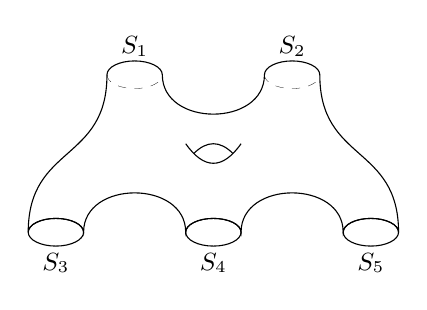
\begin{tikzpicture}[tqft/cobordism/.style={draw}]
  \pic[tqft,name=p,incoming boundary components=2,outgoing boundary components=3,genus=1,offset=-.5,every incoming lower boundary component/.style={draw,ultra thin,dashed},every outgoing boundary component/.style={draw}];
  \node[at=(p-incoming boundary 1),above=3pt,font=\small]{$S_{1}$};
  \node[at=(p-incoming boundary 2),above=3pt,font=\small]{$S_{2}$};
  \node[at=(p-outgoing boundary 1),below=4pt,font=\small]{$S_{3}$};
  \node[at=(p-outgoing boundary 2),below=4pt,font=\small]{$S_{4}$};
  \node[at=(p-outgoing boundary 3),below=4pt,font=\small]{$S_{5}$};
\end{tikzpicture}
\caption{A two-dimensional cobordism}
\label{fig:exacob}
\end{figure}
\\
We will always only draw two-dimensional examples as cobordisms in higher dimensions are difficult to draw, yet the two-dimensional pictures should make clear what we want to illustrate, even in higher dimensions. Moreover we will suppress associativity constraints. We adopt the convention that the in-boundaries are always above the out-boundaries, i.e. the cobordism goes {\glqq}top down{\grqq}. In figure \ref{fig:exacob} this means that the in-boundary is $S_{1} \sqcup S_{2}$ and the out-boundary is $S_{3} \sqcup S_{4} \sqcup S_{5}$.

\item[(ii)]
Note that the cobordisms need not be connected, thus another cobordism with the same boundaries as the one in figure \ref{fig:exacob} is pictured in figure \ref{fig:exnoncon}.
\\
\begin{figure}[h!]
\centering
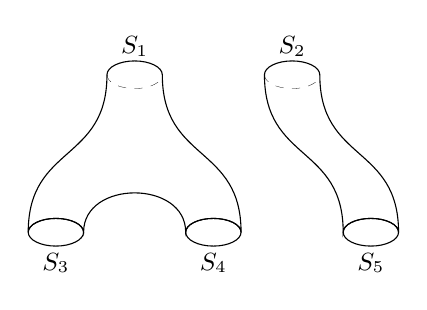
\begin{tikzpicture}[tqft/cobordism/.style={draw}]
  %left
  \pic[tqft/pair of pants,name=p,every incoming lower boundary component/.style={draw,ultra thin,dashed},every outgoing boundary component/.style={draw}];
  \node[at=(p-incoming boundary 1),above=3pt,font=\small]{$S_{1}$};
  \node[at=(p-outgoing boundary 1),below=4pt,font=\small]{$S_{3}$};
  \node[at=(p-outgoing boundary 2),below=4pt,font=\small]{$S_{4}$};
  
  %right
  \pic[tqft/cylinder to next,name=c,anchor={(0,1)},at=(p-outgoing boundary 2),every incoming lower boundary component/.style={draw,ultra thin,dashed},every outgoing boundary component/.style={draw}];
  \node[at=(c-incoming boundary 1),above=3pt,font=\small]{$S_{2}$};
  \node[at=(c-outgoing boundary 1),below=4pt,font=\small]{$S_{5}$};
\end{tikzpicture}
\caption{A non-connected two-dimensional cobordism}
\label{fig:exnoncon}
\end{figure}
\end{enumerate}
\end{exa}
Now as morphisms in $\mathbf{Cob}_{n}$ are equivalence classes of cobordisms we have to explain what equivalence means. Two cobordisms $(M,\iota_{1},\iota_{2}),(M^{\backprime},\iota_{1}^{\backprime},\iota_{2}^{\backprime})$ from $S_{1}$ to $S_{2}$ are \textbf{equivalent} if there is an orientation-preserving \textbf{diffeomorphism rel boundary}\footnote{we will sometimes also speak of a diffeomorphism that preserves the boundary} between them, that is, a diffeomorphism $\psi \colon M \to M^{\backprime}$ such that the following diagram commutes
\begin{equation*}
\begin{tikzcd}[row sep=3.2em,column sep=4em]
  &
  M
  \ar{dd}{\psi}
  &
  \\
  S_{1}
  \ar{ur}{\iota_{1}}
  \ar{dr}[swap]{\iota_{1}^{\backprime}}
  &
  &
  S_{2}
  \ar{ul}[swap]{\iota_{2}}
  \ar{dl}{\iota_{2}^{\backprime}}
  \\
  &
  M^{\backprime}
  &
\end{tikzcd}
\end{equation*}
It is evident that this is an equivalence relation and we write $[M] \doteq [(M,\iota_{1},\iota_{2})]$ for the equivalence classes. These are the morphisms of $\mathbf{Cob}_{n}$.
\\\\
The composition of two morphisms
\begin{align*}
  [(M,\iota_{1},\iota_{2})]
  \in
  \mathrm{mor}_{\mathbf{Cob}_{n}}(S_{1},S_{2})
  ,\qquad
  [(\tilde{M},\tilde{\iota}_{1},\tilde{\iota}_{2})]
  \in
  \mathrm{mor}_{\mathbf{Cob}_{n}}(S_{2},S_{3})
\end{align*}
is given by gluing the representatives $M$ and $\tilde{M}$ along $S_{2}$. More precisely let $\sim_{S_{2}}$ denote the equivalence relation in $M \sqcup \tilde{M}$ generated by the following property: two points $m \in M$ and $\tilde{m} \in \tilde{M}$ are equivalent if there is a point $s_{2} \in S_{2}$ such that
\begin{align*}
  \iota_{2}(s_{2})
  &=
  m
  \qquad
  \text{and}
  \qquad
  \tilde{\iota}_{1}(s_{2})
  =
  \tilde{m}
\end{align*}
Then the composition of morphisms
\begin{align*}
  [(\tilde{M},\tilde{\iota}_{1},\tilde{\iota}_{2})]
  \circ
  [(M,\iota_{1},\iota_{2})]
\end{align*}
is basically given by the equivalence class containing the cobordism
\begin{align*}
  M
  \sqcup_{S_{2}}
  \tilde{M}
  &:=
  (M \sqcup \tilde{M})
  /
  \sim_{S_{2}}
\end{align*}
with boundary maps
\begin{align*}
  \hat{\iota}_{1}
  \colon
  S_{1}
  &\to
  M
  \sqcup_{S_{2}}
  \tilde{M}
  ,\qquad
  \hat{\tilde{\iota}}_{2}
  \colon
  S_{3}
  \to
  M
  \sqcup_{S_{2}}
  \tilde{M}
\end{align*}
the maps obtained from $\iota_{1}$ and $\tilde{\iota}_{2}$ by extending the codomain from $M$ and $\tilde{M}$ to $M \sqcup_{S_{2}} \tilde{M}$ by composing with the maps
\begin{align*}
  j
  \colon
  M
  &\to
  M
  \sqcup_{S_{2}}
  \tilde{M}
  \qquad
  \text{and}
  \qquad
  \tilde{j}
  \colon
  \tilde{M}
  \to
  M
  \sqcup_{S_{2}}
  \tilde{M}
\end{align*}
induced on the quotient by the corresponding injections into the disjoint union. See figure \ref{fig:comp} for an illustration.
\begin{figure}[h!]
\centering
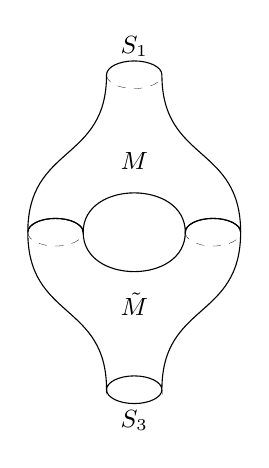
\begin{tikzpicture}[tqft/cobordism/.style={draw}]
  %top
  \pic[tqft/pair of pants,name=p,every incoming lower boundary component/.style={draw,ultra thin,dashed}];
  \node[at=(p-incoming boundary 1),above=3pt,font=\small]{$S_{1}$};
  \node[at=(p-between outgoing 1 and 2),above=5pt,font=\small]{$M$};
  
  %bottom
  \pic[tqft/reverse pair of pants,name=rp,at=(p-outgoing boundary 1),every incoming lower boundary component/.style={draw,ultra thin,dashed},every outgoing lower boundary component/.style={draw}];
  \node[at=(rp-outgoing boundary 1),below=4pt,font=\small]{$S_{3}$};
  \node[at=(rp-between incoming 1 and 2),below=4pt,font=\small]{$\tilde{M}$};
\end{tikzpicture}
\caption{Composition of two cobordisms}
\label{fig:comp}
\end{figure}
\\
One can check that this construction is the pushout
\begin{equation*}
\begin{tikzcd}[row sep=4em,column sep=4em]
  &
  &
  S_{3}
  \ar{d}{\tilde{\iota}_{2}}
  \\
  &
  S_{2}
  \ar{r}{\tilde{\iota}_{1}}
  \ar[swap]{d}{\iota_{2}}
  &
  \tilde{M}
  \ar{d}{\tilde{j}}
  \\
  S_{1}
  \ar{r}{\iota_{1}}
  &
  M
  \ar{r}{j}
  &
  M
  \sqcup_{S_{2}}
  \tilde{M}
\end{tikzcd}
\end{equation*}
in $\mathbf{Top}$, the category of topological spaces. Thus, considering everything merely as topological spaces this definition of composition does not depend on the representing cobordisms since we always have a homeomorphism respecting the boundary maps for different choices. More precisely let
\begin{align*}
  \left(
    M^{\backprime}
    ,
    \iota_{1}^{\backprime}
    ,
    \iota_{2}^{\backprime}
  \right)
  \qquad
  \text{and}
  \qquad
  \left(
    \tilde{M}^{\backprime}
    ,
    \tilde{\iota}_{1}^{\backprime}
    ,
    \tilde{\iota}_{2}^{\backprime}
  \right)
\end{align*}
be other cobordisms representing
\begin{align*}
  [(M,\iota_{1},\iota_{2})]
  \qquad
  \text{and}
  \qquad
  [(\tilde{M},\tilde{\iota}_{1},\tilde{\iota}_{2})]
\end{align*}
respectively, and let
\begin{align*}
  \psi
  \colon
  M
  &\to
  M^{\backprime}
  \qquad
  \text{and}
  \qquad
  \tilde{\psi}
  \colon
  \tilde{M}
  \to
  \tilde{M}^{\backprime}
\end{align*}
be corresponding diffeomorphis rel boundary. Then we have the following commuting diagram
\begin{equation*}
\begin{tikzcd}[row sep=5em,column sep=6em]
  S_{2}
  \ar{r}{\tilde{\iota}_{1}}
  \ar[bend left=25]{rr}{\tilde{\iota}_{1}^{\backprime}}
  \ar[swap]{d}{\iota_{2}}
  \ar[bend right=40]{dd}[swap]{\iota_{2}^{\backprime}}
  &
  \tilde{M}
  \ar{r}{\tilde{\psi}}
  \ar{d}{\tilde{j}}
  &
  \tilde{M}^{\backprime}
  \ar{dd}{\tilde{j}^{\backprime}}
  \ar[bend left=20]{l}{\tilde{\psi}^{-1}}
  \\
  M
  \ar{r}{j}
  \ar{d}[swap]{\psi}
  &
  M
  \sqcup_{S_{2}}
  \tilde{M}
  \ar[bend right=10,dashed]{rd}[swap]{\psi \sqcup_{S_{2}} \tilde{\psi}}
  \\
  M^{\backprime}
  \ar[bend right]{u}[swap]{\psi^{-1}}
  \ar{rr}{j^{\backprime}}
  &
  &
  M^{\backprime}
  \sqcup_{S_{2}}
  \tilde{M}^{\backprime}
  \ar[bend right=10,dashed]{ul}[swap]{\psi^{-1} \sqcup_{S_{2}} \tilde{\psi}^{-1}}
\end{tikzcd}
\end{equation*}
where the small square and the outer perimeter are pushouts and the dashed arrows, which can be thought of as the result of {\glqq}gluing{\grqq} $\psi,\tilde{\psi}$ and $\psi^{-1},\tilde{\psi}^{-1}$, respectively, along $S_{2}$, are the unique arrows for the corresponding pushouts. The pushout properties further imply that
\begin{align*}
  \left(
    \psi^{-1}
    \sqcup_{S_{2}}
    \tilde{\psi}^{-1}
  \right)
  \circ
  \left(
    \psi
    \sqcup_{S_{2}}
    \tilde{\psi}
  \right)
  &=
  \mathrm{id}_{M \sqcup_{S_{2}} \tilde{M}}
  \\
  \left(
    \psi
    \sqcup_{S_{2}}
    \tilde{\psi}
  \right)
  \circ
  \left(
    \psi^{-1}
    \sqcup_{S_{2}}
    \tilde{\psi}^{-1}
  \right)
  &=
  \mathrm{id}_{M^{\backprime} \sqcup_{S_{2}} \tilde{M}^{\backprime}}
\end{align*}
so that we indeed have a homeomorphism rel boundary for the glued cobordisms.
\\
Moreover, there is a canonical way to construct a continuous atlas for this topological space, so that we have the structure of topological manifolds for the composition. Note that the induced orientations on the boundaries along which the two cobordisms are glued are opposite which ensures that the orientations of the interiors are compatible with gluing. However, there is no canonical way to construct a smooth structure for $M \sqcup_{S_{2}} \tilde{M}$ from the smooth structures on $M$ and on $\tilde{M}$. Still, there is a way to endow $M \sqcup_{S_{2}} \tilde{M}$ with a smooth structure compatible with the given ones\footnote{one basically shows that one can always give the cobordisms a collar - i.e. a small neighbourhood diffeomorphic to the cylinder - at the boundary along which one wants to glue, since gluing of cylinders is easy; one might also choose the objects of $\mathbf{Cob}_{n}$ to be manifolds with collars in the first place to circumvent this problem but we do not need that here} and, with the help of morse theory, one can show that this is unique up to (non-unique) diffeomorphism, which is good enough for us since then we have the well-definedness of the composition. We do not go into the details of this construction here and instead refer the interested reader, for example, to \cite{bf5195ee} and the references therein.
\\
From this construction the associativity of the composition is not very difficult to see. On the level of topological spaces it is a consequence of the pushout property and for the smooth manifold structure it follows from the way this structure is constructed. Furthermore, it is easy to see that the identity morphism $\mathrm{id}_{S}$ for $S \in \mathrm{ob}_{\mathbf{Cob}_{n}}$ is the equivalence class that contains the cylinder $S \times [0,1]$ regarded as a cobordism from $S$ to $S$, i.e. with boundary maps induced by the identity. See figure \ref{fig:cylinder} for an illustration.
\\
\begin{figure}[h!]
\centering
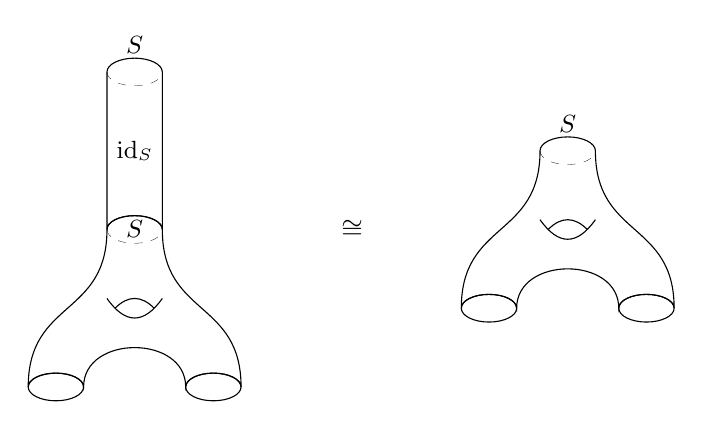
\begin{tikzpicture}[tqft/cobordism/.style={draw}]
  %left
  \pic[tqft/cylinder,name=c,every incoming lower boundary component/.style={draw,ultra thin,dashed}];
  \node[at=(c-incoming boundary 1),above=3pt,font=\small]{$S$};
  \node[at=(c-outgoing boundary 1),font=\small]{$S$};
  \node[at=(c-between first incoming and first outgoing),right,font=\small]{$\mathrm{id}_{S}$};
  \pic[tqft/pair of pants,name=g,genus=1,at=(c-outgoing boundary 1),every incoming lower boundary component/.style={draw,ultra thin,dashed},every outgoing boundary component/.style={draw}];

  %right
  \node[at=(c-outgoing boundary 1),right=2.5cm]{$\cong$};
  \pic[tqft/pair of pants,name=gc,genus=1,anchor={(-1.5,0.5)},at=(c-outgoing boundary 1),every incoming lower boundary component/.style={draw,ultra thin,dashed},every outgoing boundary component/.style={draw}];
  \node[at=(gc-incoming boundary 1),above=3pt,font=\small]{$S$};
\end{tikzpicture}
\caption{The cylinder represents the identity}
\label{fig:cylinder}
\end{figure}
\\\\\\\\\\\\
We now know that $\mathbf{Cob}_{n}$ is indeed a category, but we want to show some more, namely that it can also be given a symmetric monoidal structure. To this end, first consider the following
\\
\begin{cst}[Cylinder construction]
\label{cst:cylcst}
An orientation-preserving diffeomorphism $\phi \colon S_{1} \to S_{2}$ between two closed oriented $(n - 1)$-manifolds induces an equivalence class of cobordisms $C_{n}(\phi)$ from $S_{1}$ to $S_{2}$ via the so called cylinder construction: as a representative we can take the cylinder $S_{2} \times [0,1]$ with boundary map for $S_{1}$ the obvious map induced by $\phi$ and for $S_{2}$ the one induced by the identity. Of course we can also take $S_{1} \times [0,1]$ and use $\phi^{-1}$ for $S_{2}$ which yields an equivalent cobordism by the diffeomorphism $\phi \times \mathrm{id}_{[0,1]}$ mapping $S_{1} \times \lbrace t \rbrace$ to $S_{2} \times \lbrace t \rbrace$ by $\phi$ for each $t \in [0,1]$.
\end{cst}
\begin{prf}
Should be pretty clear.
\\
\phantom{proven}
\hfill
$\Box$
\end{prf}
Let $\mathbf{DiffCOr}_{\infty}^{n - 1}$ denote the full subcategory of $\mathbf{DiffOr}_{\infty}$ with objects $\mathrm{ob}_{\mathbf{Cob}_{n}}$ (i.e. those that are compact and have dimension $n - 1$). Then we have
\\
\begin{lem}
$C_{n}$ is a functor from $\mathbf{DiffCOr}_{\infty}^{n - 1}$ to $\mathbf{Cob}_{n}$ when defined as the identity on objects and by the cylinder construction \ref{cst:cylcst} for morphisms.
\end{lem}
\begin{prf}
\begin{enumerate}
\item[(F1)]
The identity cobordism is clearly induced by the identity diffeomorphism.

\item[(F2)]
Having two orientation-preserving diffeomorphisms
\begin{align*}
  \phi_{12}
  \colon
  S_{1}
  &\to
  S_{2}
  \qquad
  \text{and}
  \qquad
  \phi_{23}
  \colon
  S_{2}
  \to S_{3}
\end{align*}
we have to show that
\begin{align*}
  C_{n}(\phi_{23})
  \circ
  C_{n}(\phi_{12})
  &=
  C_{n}(\phi_{23} \circ \phi_{12})
\end{align*}
To this end note that by the equivalence $\phi_{23} \times \mathrm{id}_{[0,1]}$ which maps $S_{2} \times \lbrace t \rbrace$ to $S_{3} \times \lbrace t \rbrace$ by $\phi_{23}$ for each $t \in [0,1]$, we can represent $C_{n}(\phi_{12})$ by $S_{3} \times [0,1]$ with boundary maps induced by $\phi_{23} \circ \phi_{12}$ for $S_{1}$ and $\phi_{23}$ for $S_{2}$. Then by taking $S_{3} \times [0,1]$ for $C_{n}(\phi_{23})$ we can represent the compositon
\begin{align*}
  C_{n}(\phi_{23})
  \circ
  C_{n}(\phi_{12})
\end{align*}
by $S_{3} \times [0,2]$ with boundary maps induced by $\phi_{23} \circ \phi_{12}$ and $\mathrm{id}_{S_{3}}$. This latter cobordism is of course equivalent to $S_{3} \times [0,1]$ with the same boundary maps which is a representative of
\begin{align*}
  C_{n}(\phi_{23} \circ \phi_{12})
\end{align*}
\end{enumerate}
\phantom{proven}
\hfill
$\Box$
\end{prf}
It is not too difficult to show (cf. e.g. \cite{bf5195ee}) that two parallel\footnote{remember that this means that they have the same domain and codomain} diffeomorphisms induce the same equivalence class of cobordisms if and only if they are smoothly homotopic, i.e. homotopic via a smooth homotopy.
\\
Now the category $\mathbf{DiffCOr}_{\infty}^{n - 1}$ has a symmetric monoidal structure coming from its coproduct\footnote{note that every category that has finite (co)products has a monoidal structure induced from the (co)product}, the disjoint union $\sqcup$, where the unit object is the initial object, that is, the empty $(n - 1)$-manifold $\emptyset = 1_{\mathbf{DiffCOr}_{\infty}^{n - 1}}$. The associator $\mathsf{a}$ and the left and right unit law $\mathsf{l},\mathsf{r}$ are given by the obvious canonical morphisms
\begin{align*}
  \mathsf{a}(S,\tilde{S},\hat{S})
  &\colon
  \left(
    S
    \sqcup
    \tilde{S}
  \right)
  \sqcup
  \hat{S}
  \to
  S
  \sqcup
  \left(
    \tilde{S}
    \sqcup
    \hat{S}
  \right)
  \\
  \mathsf{l}(S)
  &\colon
  \emptyset
  \sqcup
  S
  \to
  S
  \\
  \mathsf{r}(S)
  &\colon
  S
  \sqcup
  \emptyset
  \to
  S
\end{align*}
for
\begin{align*}
  S
  ,
  \tilde{S}
  ,
  \hat{S}
  \in
  \mathrm{ob}_{\mathbf{Cob}_{n}}
  &=
  \mathrm{ob}_{\mathbf{DiffCOr}_{\infty}^{n - 1}}
\end{align*}
It is pretty clear that these are natural and satisfy the coherence conditions so we will not go into further detail here. The braiding $\mathsf{b}$ is given by the canonical morphisms
\begin{align*}
  \mathsf{b}(S,\tilde{S})
  \colon
  S
  \sqcup
  \tilde{S}
  &\to
  \tilde{S}
  \sqcup
  S
\end{align*}
and it is again pretty obvious that this is natural and satisfies the hexagon equations. Moreover, it is evident that this braiding is symmteric. From this symmetric monoidal structure the cylinder construction $C_{n}$ induces a symmetric monoidal structure on $\mathbf{Cob}_{n}$ as described below.
\\
The tensor product in $\mathbf{Cob}_{n}$ is given by the disjoint union $\sqcup$. The disjoint union of two equivalence classes of cobordisms
\begin{align*}
  [(M,\iota_{1},\iota_{2})]
  \in
  \mathrm{mor}_{\mathbf{Cob}_{n}}(S_{1},S_{2})
  \qquad
  \text{and}
  \qquad
  [(\tilde{M},\tilde{\iota}_{1},\tilde{\iota}_{2})]
  \in
  \mathrm{mor}_{\mathbf{Cob}_{n}}(\tilde{S}_{1},\tilde{S}_{2})
\end{align*}
is the equivalence class of cobordisms of the disjoint union of a representative from each class, i.e.
\begin{align*}
  [(M,\iota_{1},\iota_{2})] \sqcup [(\tilde{M},\tilde{\iota}_{1},\tilde{\iota}_{2})]
  &:=
  [(M \sqcup \tilde{M},\iota_{1} \sqcup \tilde{\iota}_{1},\iota_{2} \sqcup \tilde{\iota}_{2})]
  \in
  \mathrm{mor}_{\mathbf{Cob}_{n}}(S_{1} \sqcup \tilde{S}_{1},S_{2} \sqcup \tilde{S}_{2})
\end{align*}
This does not depend on the chosen representatives since for other representatives
\begin{align*}
  M^{\backprime}
  \in
  [M]
  \qquad
  \text{and}
  \qquad
  \tilde{M}^{\backprime}
  \in
  [\tilde{M}]
\end{align*}
we have equivalences
\begin{align*}
  \psi
  \colon
  M
  &\to
  M^{\backprime}
  \qquad
  \text{and}
  \qquad
  \tilde{\psi}
  \colon
  \tilde{M}
  \to
  \tilde{M}^{\backprime}
\end{align*}
respectively, and together they give an equivalence between the disjoint unions
\begin{align*}
  \psi
  \sqcup
  \tilde{\psi}
  &\colon
  M
  \sqcup
  \tilde{M}
  \to
  M^{\backprime}
  \sqcup
  \tilde{M}^{\backprime}
\end{align*}
To show that this really yields a tensor product on $\mathbf{Cob}_{n}$ we need the following
\\
\begin{lem}
\label{lem:disunfun}
Taking the disjoint union of manifolds on the level of objects and the disjoint union of equivalence classes of cobordisms on the level of morphisms yields a functor
\begin{align*}
  \cdot
  \sqcup
  \cdot
  \doteq
  \sqcup
  \colon
  \mathbf{Cob}_{n}
  \times
  \mathbf{Cob}_{n}
  &\to
  \mathbf{Cob}_{n}
\end{align*}
We use infix notation for this functor as is usual for disjoint unions.
\end{lem}
\begin{prf}
\begin{enumerate}
\item[(F1)]
For $S_{1},S_{2} \in \mathrm{ob}_{\mathbf{Cob}_{n}}$ it is clear that there is an equivalence of cobordisms between the cylinders
\begin{align*}
  \left(
    S_{1}
    \times
    [0,1]
  \right)
  \sqcup
  \left(
    S_{2}
    \times
    [0,1]
  \right)
\end{align*}
and
\begin{align*}
  \left(
    S_{1}
    \sqcup
    S_{2}
  \right)
  \times
  [0,1]
\end{align*}
Hence we have
\begin{align*}
  \mathrm{id}_{S_{1}}
  \sqcup
  \mathrm{id}_{S_{2}}
  &=
  \mathrm{id}_{S_{1} \sqcup S_{2}}
\end{align*}

\item[(F2)]
Given two pairs of cobordisms such that each pair consists of two cobordisms which can be glued together,
\begin{align*}
  (M^{12},\iota_{1}^{12},\iota_{2}^{12})
  \colon
  S_{1}
  &\to
  S_{2}
  ,\qquad
  (M^{23},\iota_{1}^{23},\iota_{2}^{23})
  \colon
  S_{2}
  \to
  S_{3}
  \\
  (\tilde{M}^{12},\tilde{\iota}_{1}^{12},\tilde{\iota}_{2}^{12})
  \colon
  \tilde{S}_{1}
  &\to
  \tilde{S}_{2}
  ,\qquad
  (\tilde{M}^{23},\tilde{\iota}_{1}^{23},\tilde{\iota}_{2}^{23})
  \colon
  \tilde{S}_{2}
  \to
  \tilde{S}_{3}
\end{align*}
Then we can first do the gluing of each pair and then take the disjoint union or we can first take the disjoint unions seperately and then glue these disjoint unions together,
\begin{align*}
  \left(
    M^{12}
    \sqcup_{S_{2}}
    M^{23}
  \right)
  \sqcup
  \left(
    \tilde{M}^{12}
    \sqcup_{\tilde{S}_{2}}
    \tilde{M}^{23}
  \right)
  \colon
  S_{1}
  \sqcup
  \tilde{S}_{1}
  &\to
  S_{3}
  \sqcup
  \tilde{S}_{3}
  \\
  \text{with}
  \qquad
  \widehat{\iota_{1}^{12}}
  \sqcup
  \widehat{\tilde{\iota}_{1}^{12}}
  \qquad
  \text{and}
  \qquad
  \widehat{\iota_{2}^{23}}
  \sqcup
  \widehat{\tilde{\iota}_{2}^{23}}
\end{align*}
or
\begin{align*}
  \left(
    M^{12}
    \sqcup
    \tilde{M}^{12}
  \right)
  \sqcup_{S_{2} \sqcup \tilde{S}_{2}}
  \left(
    M^{23}
    \sqcup
    \tilde{M}^{23}
  \right)
  \colon
  S_{1}
  \sqcup
  \tilde{S}_{1}
  &\to
  S_{3}
  \sqcup
  \tilde{S}_{3}
  \\
  \text{with}
  \qquad
  \widehat{\iota_{1}^{12} \sqcup \tilde{\iota}_{1}^{12}}
  \qquad
  \text{and}
  \qquad
  \widehat{\iota_{2}^{23} \sqcup \tilde{\iota}_{2}^{23}}
\end{align*}
But there clearly is a diffeomorphism respecting the boundary maps between the resulting cobordisms, making them equivalent. For an illustration see figure \ref{fig:disunfun}
\\
\begin{figure}[h!]
\centering
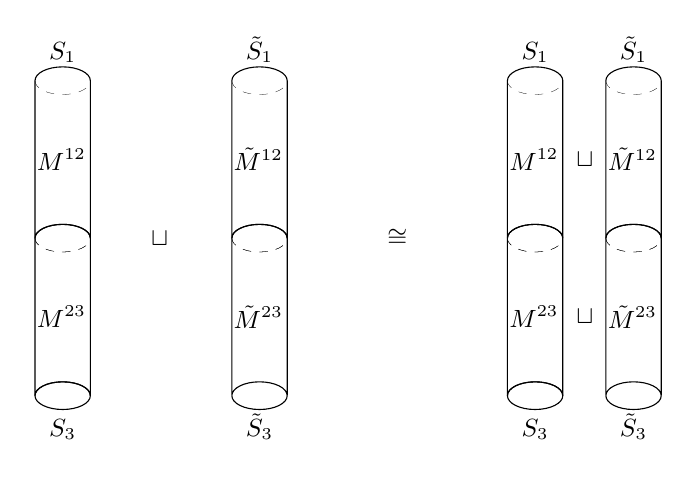
\begin{tikzpicture}[tqft/cobordism/.style={draw}]
  %left
  %upper
  \pic[tqft/cylinder,name=l,boundary separation=2.5cm,every incoming lower boundary component/.style={draw,ultra thin,dashed},every outgoing boundary component/.style={draw,ultra thin,dashed}];
  \node[at=(l-incoming boundary 1),above=3pt,font=\small]{$S_{1}$};
  \node[at=(l-between first incoming and first outgoing),right=-1mm,font=\small]{$M^{12}$};
  \pic[tqft/cylinder,name=r,boundary separation=2.5cm,anchor={(0,0)},at=(l-incoming boundary 1),every incoming lower boundary component/.style={draw,ultra thin,dashed},every outgoing lower boundary component/.style={draw,ultra thin,dashed}];
  \node[at=(r-incoming boundary 1),above=3pt,font=\small]{$\tilde{S}_{1}$};
  \node[at=(r-between first incoming and first outgoing),right=-1mm,font=\small]{$\tilde{M}^{12}$};
  \node[at=(l-outgoing boundary 1),right=1cm,font=\small]{$\sqcup$};
  %lower
  \pic[tqft/cylinder,name=l2,boundary separation=2.5cm,at=(l-outgoing boundary 1),every incoming lower boundary component/.style={draw,ultra thin,dashed},every outgoing boundary component/.style={draw}];
  \node[at=(l2-outgoing boundary 1),below=5pt,font=\small]{$S_{3}$};
  \node[at=(l2-between first incoming and first outgoing),right=-1mm,font=\small]{$M^{23}$};
  \pic[tqft/cylinder,name=r2,boundary separation=2.5cm,at=(r-outgoing boundary 1),every incoming lower boundary component/.style={draw,ultra thin,dashed},every outgoing lower boundary component/.style={draw}];
  \node[at=(r2-outgoing boundary 1),below=3pt,font=\small]{$\tilde{S}_{3}$};
  \node[at=(r2-between first incoming and first outgoing),right=-1mm,font=\small]{$\tilde{M}^{23}$};

  %right
  \node[at=(r-outgoing boundary 1),right=1.5cm,font=\small]{$\cong$};
  %upper
  \pic[tqft/cylinder,name=lu,boundary separation=2.5cm,anchor={(-1.4,0)},every incoming lower boundary component/.style={draw,ultra thin,dashed},every outgoing boundary component/.style={draw,ultra thin,dashed}];
  \node[at=(lu-incoming boundary 1),above=3pt,font=\small]{$S_{1}$};
  \node[at=(lu-between first incoming and first outgoing),right=-1mm,font=\small]{$M^{12}$};
  \node[at=(lu-between first incoming and first outgoing),right=0.75cm,font=\small]{$\sqcup$};
  \pic[tqft/cylinder,name=ru,boundary separation=2.5cm,anchor={(0.5,0)},at=(lu-incoming boundary 1),every incoming lower boundary component/.style={draw,ultra thin,dashed},every outgoing lower boundary component/.style={draw,ultra thin,dashed}];
  \node[at=(ru-incoming boundary 1),above=3pt,font=\small]{$\tilde{S}_{1}$};
  \node[at=(ru-between first incoming and first outgoing),right=-1mm,font=\small]{$\tilde{M}^{12}$};

  %lower
  \pic[tqft/cylinder,name=ll,boundary separation=2.5cm,at=(lu-outgoing boundary 1),every incoming lower boundary component/.style={draw,ultra thin,dashed},every outgoing boundary component/.style={draw}];
  \node[at=(ll-outgoing boundary 1),below=5pt,font=\small]{$S_{3}$};
  \node[at=(ll-between first incoming and first outgoing),right=-1mm,font=\small]{$M^{23}$};
  \node[at=(ll-between first incoming and first outgoing),right=0.75cm,font=\small]{$\sqcup$};
  \pic[tqft/cylinder,name=rl,boundary separation=2.5cm,at=(ru-outgoing boundary 1),every incoming lower boundary component/.style={draw,ultra thin,dashed},every outgoing lower boundary component/.style={draw}];
  \node[at=(rl-outgoing boundary 1),below=3pt,font=\small]{$\tilde{S}_{3}$};
  \node[at=(rl-between first incoming and first outgoing),right=-1mm,font=\small]{$\tilde{M}^{23}$};
\end{tikzpicture}
\caption{Illustration of the functoriality of the disjoint union}
\label{fig:disunfun}
\end{figure}
\\
This implies the compatibility with composition
\begin{align*}
  \left(
    [M^{23}]
    \circ
    [M^{12}]
  \right)
  \sqcup
  \left(
    [\tilde{M}^{23}]
    \circ
    [\tilde{M}^{12}]
  \right)
  &=
  \left(
    [M^{23}]
    \sqcup
    [\tilde{M}^{23}]
  \right)
  \circ
  \left(
    [M^{12}]
    \sqcup
    [\tilde{M}^{12}]
  \right)
\end{align*}
\end{enumerate}
\phantom{proven}
\hfill
$\Box$
\end{prf}
The unit object for the symmetric monoidal structure is the empty $(n - 1)$-manifold
\begin{align*}
  \emptyset
  &=
  1_{\mathbf{Cob}_{n}}
  =
  1_{\mathbf{DiffCOr}_{\infty}^{n - 1}}
\end{align*}
The associator $\mathsf{A}$ and the left and right unit law $\mathsf{L},\mathsf{R}$ are obtained from the cylinder construction for the associator and the unit laws in $\mathbf{DiffCOr}_{\infty}^{n - 1}$, i.e.
\begin{align*}
  \mathsf{A}(S,\tilde{S},\hat{S})
  &:=
  C_{n}(\mathsf{a}(S,\tilde{S},\hat{S}))
  ,\qquad
  \mathsf{L}(S)
  :=
  C_{n}(\mathsf{l}(S))
  ,\qquad
  \mathsf{R}(S)
  :=
  C_{n}(\mathsf{r}(S))
\end{align*}
for
\begin{align*}
  S
  ,
  \tilde{S}
  ,
  \hat{S}
  \in
  \mathrm{ob}_{\mathbf{Cob}_{n}}
  &=
  \mathrm{ob}_{\mathbf{DiffCOr}_{\infty}^{n - 1}}
\end{align*}
Note that since $\emptyset \sqcup \emptyset = \emptyset$, we have
\begin{align*}
  \mathsf{l}(\emptyset)
  &=
  \mathsf{r}(\emptyset)
  =
  \mathrm{id}_{\emptyset}
  \in
  \mathrm{mor}_{\mathbf{DiffCOr}_{\infty}^{n-1}}
  \left(
    \emptyset
    ,
    \emptyset
  \right)
\end{align*}
and thus
\begin{align*}
  \mathsf{L}(\emptyset)
  &=
  \mathsf{R}(\emptyset)
  =
  \mathrm{id}_{\emptyset}
  \in
  \mathrm{mor}_{\mathbf{Cob}_{n}}
  \left(
    \emptyset
    ,
    \emptyset
  \right)
\end{align*}
where this latter $\mathrm{id}_{\emptyset}$ is the equivalence class containing the empty $n$-manifold as cobordism\footnote{this is the only cobordism in this equivalence class, of course, and the boundary maps are the empty maps}.
\\
For the naturality of $\mathsf{A}$ let
\begin{align*}
  [(M,\iota_{1},\iota_{2})]
  &\in
  \mathrm{mor}_{\mathbf{Cob}_{n}}(S_{1},S_{2})
  \\
  [(\tilde{M},\tilde{\iota}_{1},\tilde{\iota}_{2})]
  &\in
  \mathrm{mor}_{\mathbf{Cob}_{n}}(\tilde{S}_{1},\tilde{S}_{2})
  \\
  [(\hat{M},\hat{\iota}_{1},\hat{\iota}_{2})]
  &\in
  \mathrm{mor}_{\mathbf{Cob}_{n}}(\hat{S}_{1},\hat{S}_{2})
\end{align*}
then we want to show that
\begin{align*}
  \left(
    [M]
    \sqcup
    [\tilde{M}]
  \right)
  \sqcup
  [\hat{M}]
  &=
  \mathsf{A}^{-1}(S_{2},\tilde{S}_{2},\hat{S}_{2})
  \circ
  \left(
    [M]
    \sqcup
    \left(
      [\tilde{M}]
      \sqcup
      [\hat{M}]
    \right)
  \right)
  \circ
  \mathsf{A}(S_{1},\tilde{S}_{1},\hat{S}_{1})
\end{align*}
The equivalence class on the left can be represented by the cobordism
\begin{align*}
  \left(
    (M \sqcup \tilde{M})
    \sqcup
    \hat{M}
    ,
    (\iota_{1} \sqcup \tilde{\iota}_{1})
    \sqcup
    \hat{\iota}_{1}
    ,
    (\iota_{2} \sqcup \tilde{\iota}_{2})
    \sqcup
    \hat{\iota}_{2}
  \right)
\end{align*}
and the one on the right can be represented by
\begin{align*}
  \left(
    M
    \sqcup
    (\tilde{M} \sqcup \hat{M})
    ,
    (\iota_{1} \sqcup (\tilde{\iota}_{1} \sqcup \hat{\iota}_{1}))
    \circ
    \mathsf{a}(S_{1},\tilde{S}_{1},\hat{S}_{1})
    ,
    (\iota_{2} \sqcup (\tilde{\iota}_{2} \sqcup \hat{\iota}_{2}))
    \circ
    \mathsf{a}(S_{2},\tilde{S}_{2},\hat{S}_{2})
  \right)
\end{align*}
because we can diffeomorphically collapse the attached cylinders that represent the associators
\begin{align*}
  \mathsf{A}^{-1}(S_{2},\tilde{S}_{2},\hat{S}_{2})
  \qquad
  \text{and}
  \qquad
  \mathsf{A}(S_{1},\tilde{S}_{1},\hat{S}_{1})
\end{align*}
and this collapsing results in simply adapting the boundary maps of the cobordisms without the cylinders for the associators. Thus we need a diffeomorphism
\begin{align*}
  \psi
  \colon
  (M \sqcup \tilde{M})
  \sqcup
  \hat{M}
  \to
  M
  \sqcup
  (\tilde{M} \sqcup \hat{M})
\end{align*}
which makes the following diagram commute
\begin{equation*}
\begin{tikzcd}[column sep=1.4em]
  &
  &
  (M \sqcup \tilde{M}) \sqcup \hat{M}
  \ar{dddd}{\psi}
  &
  &
  \\
  \\
  (S_{1} \sqcup \tilde{S}_{1}) \sqcup \hat{S}_{1}
  \ar{uurr}{(\iota_{1} \sqcup \tilde{\iota}_{1}) \sqcup \hat{\iota}_{1}}
  \ar{dr}[swap]{\mathsf{a}(S_{1},\tilde{S}_{1},\hat{S}_{1})}
  &
  &
  &
  &
  (S_{2} \sqcup \tilde{S}_{2}) \sqcup \hat{S}_{2}
  \ar{uull}[swap]{(\iota_{2} \sqcup \tilde{\iota}_{2}) \sqcup \hat{\iota}_{2}}
  \ar{dl}{\mathsf{a}(S_{2},\tilde{S}_{2},\hat{S}_{2})}
  \\
  &
  S_{1} \sqcup (\tilde{S}_{1} \sqcup \hat{S}_{1})
  \ar{dr}[swap]{\iota_{1} \sqcup (\tilde{\iota}_{1} \sqcup \hat{\iota}_{1})}
  &
  &
  S_{2} \sqcup (\tilde{S}_{2} \sqcup \hat{S}_{2})
  \ar{dl}{\iota_{2} \sqcup (\tilde{\iota}_{2} \sqcup \hat{\iota}_{2})}
  &
  \\
  &
  &
  M \sqcup (\tilde{M} \sqcup \hat{M})
  &
  &
\end{tikzcd}
\end{equation*}
But the canonical diffeomorphism clearly does the job. A similar argument shows the naturality of $\mathsf{L}$ and $\mathsf{R}$.
\\
The braiding $\mathsf{B}$ in $\mathbf{Cob}_{n}$ also comes from the braiding in $\mathbf{DiffCOr}_{\infty}^{n - 1}$ by the cylinder construction,
\begin{align*}
  \mathsf{B}(S,\tilde{S})
  &:=
  C_{n}(\mathsf{b}(S,\tilde{S}))
\end{align*}
This braiding is symmetric since $\mathsf{b}$ is symmetric and thus
\begin{align*}
  \mathsf{B}(\tilde{S},S)
  &=
  C_{n}(\mathsf{b}(\tilde{S},S))
  \\
  &=
  C_{n}(\mathsf{b}(S,\tilde{S})^{-1})
  \\
  &=
  C_{n}(\mathsf{b}(S,\tilde{S}))^{-1}
  \\
  &=
  \mathsf{B}(S,\tilde{S})^{-1}
\end{align*}
The naturality of $\mathsf{B}$ follows again by a similar reasoning as above. We will usually depict the braiding as in figure \ref{fig:braiding} which illustrates the symmetry. Note however that there is not really an intersection of the components, it just illustrates that it does not make sense to talk about crossing over or under as the manifolds considered are abstract and not embedded into a surrounding space.
\\
\begin{figure}[h!]
\centering
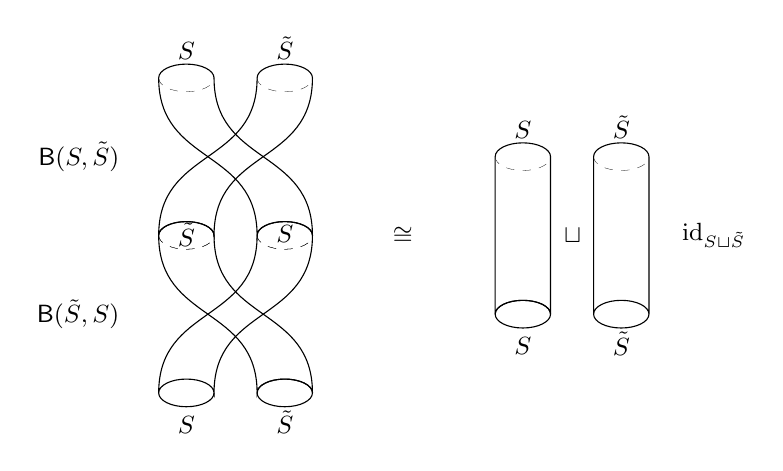
\begin{tikzpicture}[tqft/cobordism/.style={draw}]
  %left
  %upper braiding
  \pic[tqft/cylinder to next,name=l,boundary separation=2.5cm,every incoming lower boundary component/.style={draw,ultra thin,dashed},every outgoing boundary component/.style={draw,ultra thin,dashed}];
  \node[at=(l-incoming boundary 1),above=3pt,font=\small]{$S$};
  \node[at=(l-outgoing boundary 1),below=-7pt,font=\small]{$S$};
  \pic[tqft/cylinder to prior,name=r,boundary separation=2.5cm,anchor={(0.5,0)},at=(l-incoming boundary 1),every incoming lower boundary component/.style={draw,ultra thin,dashed},every outgoing lower boundary component/.style={draw,ultra thin,dashed}];
  \node[at=(r-incoming boundary 1),above=3pt,font=\small]{$\tilde{S}$};
  \node[at=(r-outgoing boundary 1),below=-8pt,font=\small]{$\tilde{S}$};
  \node[at=(r-between first incoming and first outgoing),left=1cm,font=\small]{$\mathsf{B}(S,\tilde{S})$};
  %lower braiding
  \pic[tqft/cylinder to next,name=l2,boundary separation=2.5cm,at=(r-outgoing boundary 1),every incoming lower boundary component/.style={draw,ultra thin,dashed},every outgoing boundary component/.style={draw}];
  \node[at=(l2-outgoing boundary 1),below=3pt,font=\small]{$\tilde{S}$};
  \pic[tqft/cylinder to prior,name=r2,boundary separation=2.5cm,at=(l-outgoing boundary 1),every incoming lower boundary component/.style={draw,ultra thin,dashed},every outgoing lower boundary component/.style={draw}];
  \node[at=(r2-outgoing boundary 1),below=5pt,font=\small]{$S$};
  \node[at=(r2-between first incoming and first outgoing),left=1cm,font=\small]{$\mathsf{B}(\tilde{S},S)$};

  %right
  \node[at=(r-outgoing boundary 1),right=2.5cm,font=\small]{$\cong$};
  %upper cylinder
  \pic[tqft/cylinder,name=lc,boundary separation=2.5cm,anchor={(-0.6,0)},at=(r-between first incoming and first outgoing),every incoming lower boundary component/.style={draw,ultra thin,dashed},every outgoing boundary component/.style={draw}];
  \node[at=(lc-incoming boundary 1),above=3pt,font=\small]{$S$};
  \node[at=(lc-outgoing boundary 1),below=5pt,font=\small]{$S$};
  \node[at=(lc-between first incoming and first outgoing),right=0.75cm,font=\small]{$\sqcup$};
  %lower cylinder
  \pic[tqft/cylinder,name=rc,boundary separation=2.5cm,anchor={(0.5,0)},at=(lc-incoming boundary 1),every incoming lower boundary component/.style={draw,ultra thin,dashed},every outgoing lower boundary component/.style={draw}];
  \node[at=(rc-incoming boundary 1),above=3pt,font=\small]{$\tilde{S}$};
  \node[at=(rc-outgoing boundary 1),below=3pt,font=\small]{$\tilde{S}$};
  \node[at=(rc-between first incoming and first outgoing),right=1cm,font=\small]{$\mathrm{id}_{S \sqcup \tilde{S}}$};
\end{tikzpicture}
\caption{Illustration of the symmetry of the braiding}
\label{fig:braiding}
\end{figure}
\newpage
The pentagon, triangle and hexagon equations follow from the cylinder construction applied to the corresponding equations in $\mathbf{DiffCOr}_{\infty}^{n - 1}$ because the cylinder construction preserves the disjoint union, i.e. as functors we have
\begin{align*}
  C_{n}
  \circ
  \sqcup
  &=
  \sqcup
  \circ
  (C_{n} \times C_{n})
\end{align*}
On the level of objects this is obvious since $C_{n}$ is the identity there. On the level of morphisms we need to show
\begin{align*}
  C_{n}(\phi \sqcup \tilde{\phi})
  &=
  C_{n}(\phi)
  \sqcup
  C_{n}(\tilde{\phi})
\end{align*}
for
\begin{align*}
  \phi
  \in
  \mathrm{mor}_{\mathbf{DiffCOr}_{\infty}^{n - 1}}
  \left(
    S_{1}
    ,
    S_{2}
  \right)
  ,\qquad
  \tilde{\phi}
  \in
  \mathrm{mor}_{\mathbf{DiffCOr}_{\infty}^{n - 1}}
  \left(
    \tilde{S}_{1}
    ,
    \tilde{S}_{2}
  \right)
\end{align*}
But this is true because the left-hand side can be represented by the cobordism
\begin{align*}
  (S_{2} \sqcup \tilde{S}_{2})
  \times
  [0,1]
\end{align*}
and the right-hand side by
\begin{align*}
  (S_{2} \times [0,1])
  \sqcup
  (\tilde{S}_{2} \times [0,1])
\end{align*}
and we have a canoncial diffeomorphism between them which is a diffeomorphism rel boundary. Note that this also implies that
\begin{align*}
  \left(
    C_{n}
    ,
    \mathrm{id}_{C_{n} \circ \sqcup}
    ,
    \mathrm{id}_{\emptyset}
  \right)
  \colon
  \left(
    \mathbf{DiffCOr}_{\infty}^{n-1}
    ,
    \sqcup
    ,
    \mathsf{a}
    ,
    \emptyset
    ,
    \mathsf{l}
    ,
    \mathsf{r}
    ,
    \mathsf{b}
  \right)
  &\to
  \left(
    \mathbf{Cob}_{n}
    ,
    \sqcup
    ,
    \mathsf{A}
    ,
    \emptyset
    ,
    \mathsf{L}
    ,
    \mathsf{R}
    ,
    \mathsf{B}
  \right)
\end{align*}
is a symmetric monoidal functor.
\\\\
The category $\mathbf{Cob}_{n}$ has another important property: it is rigid, that is, for every $S \in \mathrm{ob}_{\mathbf{Cob}_{n}}$ there is a dual object in $\mathbf{Cob}_{n}$.
\\
\begin{lem}
\label{lem:cobrigid}
For every object $S \in \mathrm{ob}_{\mathbf{Cob}_{n}}$ there is a left dual object in $\mathbf{Cob}_{n}$ given by the manifold with reversed orientation $\overline{S}$. The evaluation
\begin{align*}
  \mathrm{ev}_{S}
  \colon
  \overline{S}
  \sqcup
  S
  &\to
  \emptyset
\end{align*}
and coevaluation
\begin{align*}
  \mathrm{coev}_{S}
  \colon
  \emptyset
  &\to
  S
  \sqcup
  \overline{S}
\end{align*}
are each given by the equivalence class of the cylinder $S \times [0,1]$ regarded as cobordism with empty out-boundary and empty in-boundary, respectively. As $\mathbf{Cob}_{n}$ is braided monoidal such a left dual object is also a right dual object with the appropriately adapted evaluation and coevaluation. Hence $\mathbf{Cob}_{n}$ is rigid.
\end{lem}
\begin{prf}[Sketch]
We can think of the evaluation and coevaluation as {\glqq}bent cylinders{\grqq} and will depict them as in figure \ref{fig:evcoev}.
\\
\begin{figure}[h!]
\centering
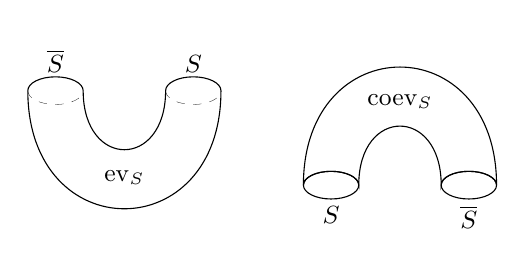
\begin{tikzpicture}[tqft/cobordism/.style={draw}]
  %left
  \pic[tqft,name=ev,cobordism height=3cm,boundary separation=1.75cm,incoming boundary components=2,outgoing boundary components=0,every incoming lower boundary component/.style={draw,ultra thin,dashed}];
  \node[at=(ev-incoming boundary 1),above=3pt,font=\small]{$\overline{S}$};
  \node[at=(ev-incoming boundary 2),above=3pt,font=\small]{$S$};
  \node[at=(ev-between incoming 1 and 2),below=4pt,font=\small]{$\mathrm{ev}_{S}$};

  %right
  \pic[tqft,name=co,cobordism height=3cm,boundary separation=1.75cm,incoming boundary components=0,outgoing boundary components=2,anchor={(0,0.6)},at=(ev-incoming boundary 2),every outgoing boundary component/.style={draw}];
  \node[at=(co-outgoing boundary 1),below=4pt,font=\small]{$S$};
  \node[at=(co-outgoing boundary 2),below=4pt,font=\small]{$\overline{S}$};
  \node[at=(co-between outgoing 1 and 2),above=3pt,font=\small]{$\mathrm{coev}_{S}$};
\end{tikzpicture}
\caption{Illustration of the evaluation and coevaluation}
\label{fig:evcoev}
\end{figure}
\\
They have to make the diagrams (LD1) and (LD2) for dual objects commute, i.e.
\begin{equation*}
\begin{tikzcd}
  \emptyset \sqcup S
  \ar{rr}{\mathsf{L}(S)}
  \ar{dd}[swap]{\mathrm{coev}_{S} \sqcup \mathrm{id}_{S}}
  &
  &
  S
  &
  &
  S \sqcup \emptyset
  \ar{ll}[swap]{\mathsf{R}(S)}
  \\
  \\
  (S \sqcup \overline{S}) \sqcup S
  \ar{rrrr}{\mathsf{A}(S,\overline{S},S)}
  &
  &
  &
  &
  S \sqcup (\overline{S} \sqcup S)
  \ar{uu}[swap]{\mathrm{id}_{S} \sqcup \mathrm{ev}_{S}}
\end{tikzcd}
\end{equation*}
\begin{equation*}
\begin{tikzcd}
  \overline{S} \sqcup \emptyset
  \ar{rr}{\mathsf{R}(\overline{S})}
  \ar{dd}[swap]{\mathrm{id}_{\overline{S}} \sqcup \mathrm{coev}_{S}}
  &
  &
  \overline{S}
  &
  &
  \emptyset \sqcup \overline{S}
  \ar{ll}[swap]{\mathsf{L}(\overline{S})}
  \\
  \\
  \overline{S} \sqcup (S \sqcup \overline{S})
  \ar{rrrr}{\mathsf{A}^{-1}(\overline{S},S,\overline{S})}
  &
  &
  &
  &
  (\overline{S} \sqcup S) \sqcup \overline{S}
  \ar{uu}[swap]{\mathrm{ev}_{S} \sqcup \mathrm{id}_{\overline{S}}}
\end{tikzcd}
\end{equation*}
Since $\mathsf{L}$, $\mathsf{R}$ and $\mathsf{A}$ can be represented by cylinders this is rather clear because we can collapse the cylinders which, as before, results in simply adjusting the boundary maps. Then the composition of the cobordisms in the given way is just gluing bent and unbent cylinders in the appropriate way to form a cobordism again diffeomorphic to an unbent cylinder as illustrated for the first diagram in figure \ref{fig:dualobcob1} and for the second diagram in figure \ref{fig:dualobcob2}.
\\
\begin{figure}[h!]
\centering
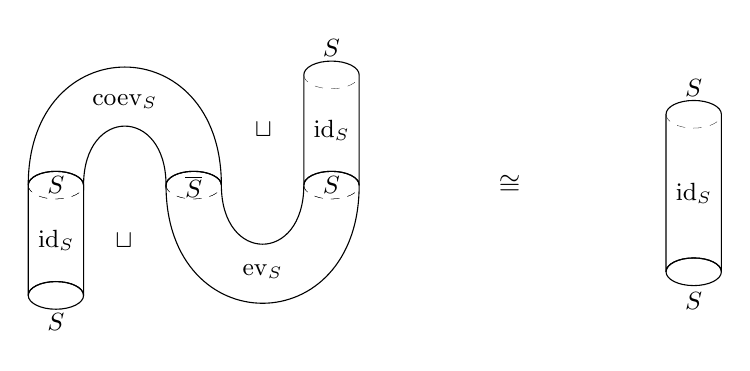
\begin{tikzpicture}[tqft/cobordism/.style={draw}]
  %left
  %coevaluation
  \pic[tqft,name=co,cobordism height=3cm,boundary separation=1.75cm,incoming boundary components=0,outgoing boundary components=2,every outgoing boundary component/.style={draw,ultra thin,dashed}];
  \node[at=(co-outgoing boundary 1),font=\small]{$S$};
  \node[at=(co-outgoing boundary 2),below=-7pt,font=\small]{$\overline{S}$};
  \node[at=(co-between outgoing 1 and 2),above=3pt,font=\small]{$\mathrm{coev}_{S}$};
  %evaluation
  \pic[tqft,name=ev,cobordism height=3cm,boundary separation=1.75cm,incoming boundary components=2,outgoing boundary components=0,anchor=incoming boundary 1,at=(co-outgoing boundary 2),every incoming lower boundary component/.style={draw,ultra thin,dashed}];
  \node[at=(ev-incoming boundary 2),font=\small]{$S$};
  \node[at=(ev-between incoming 1 and 2),below=4pt,font=\small]{$\mathrm{ev}_{S}$};
  %cylinders
  \pic[tqft/cylinder,name=c1,cobordism height=1.4cm,anchor=outgoing boundary 1,at=(ev-incoming boundary 2),every incoming lower boundary component/.style={draw,ultra thin,dashed},every outgoing boundary component/.style={draw,ultra thin,dashed}];
  \node[at=(c1-incoming boundary 1),above=3pt,font=\small]{$S$};
  \node[at=(c1-between first incoming and first outgoing),right,font=\small]{$\mathrm{id}_{S}$};
  \node[at=(c1-between first incoming and first outgoing),left=8pt,font=\small]{$\sqcup$};
  \pic[tqft/cylinder,name=c2,cobordism height=1.4cm,anchor=incoming boundary 1,at=(co-outgoing boundary 1),every incoming lower boundary component/.style={draw,ultra thin,dashed},every outgoing boundary component/.style={draw}];
  \node[at=(c2-outgoing boundary 1),below=3pt,font=\small]{$S$};
  \node[at=(c2-between first incoming and first outgoing),right,font=\small]{$\mathrm{id}_{S}$};
  \node[at=(c2-between last incoming and last outgoing),right=8pt,font=\small]{$\sqcup$};
  
  %right
  \node[at=(c1-outgoing boundary 1),right=2cm]{$\cong$};
  \pic[tqft/cylinder,name=c,anchor={(-1.3,-0.25)},at=(c1-incoming boundary 1),every incoming lower boundary component/.style={draw,ultra thin,dashed},every outgoing boundary component/.style={draw}];
  \node[at=(c-incoming boundary 1),above=3pt,font=\small]{$S$};
  \node[at=(c-outgoing boundary 1),below=4pt,font=\small]{$S$};
  \node[at=(c-between first incoming and first outgoing),right,font=\small]{$\mathrm{id}_{S}$};
\end{tikzpicture}
\caption{Illustration of the first diagram for dual objects}
\label{fig:dualobcob1}
\end{figure}
\\
\begin{figure}[h!]
\centering
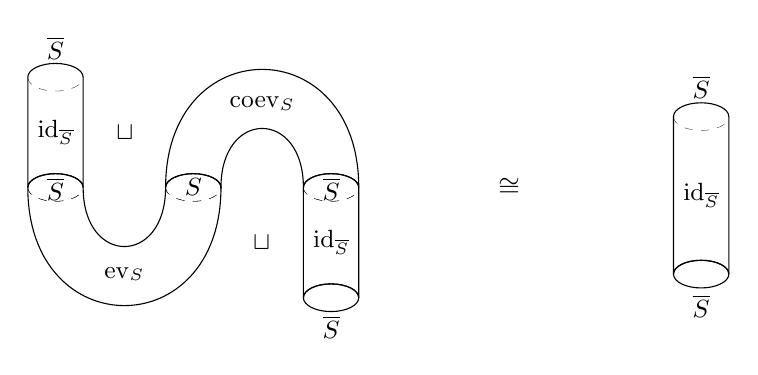
\begin{tikzpicture}[tqft/cobordism/.style={draw}]
  %left
  %coevaluation
  \pic[tqft,name=co,cobordism height=3cm,boundary separation=1.75cm,incoming boundary components=0,outgoing boundary components=2,every outgoing boundary component/.style={draw,ultra thin,dashed}];
  \node[at=(co-outgoing boundary 1),font=\small]{$S$};
  \node[at=(co-outgoing boundary 2),below=-7pt,font=\small]{$\overline{S}$};
  \node[at=(co-between outgoing 1 and 2),above=3pt,font=\small]{$\mathrm{coev}_{S}$};
  %evaluation
  \pic[tqft,name=ev,cobordism height=3cm,boundary separation=1.75cm,incoming boundary components=2,outgoing boundary components=0,anchor=incoming boundary 2,at=(co-outgoing boundary 1),every incoming lower boundary component/.style={draw,ultra thin,dashed}];
  \node[at=(ev-incoming boundary 1),below=-7pt,font=\small]{$\overline{S}$};
  \node[at=(ev-between incoming 1 and 2),below=4pt,font=\small]{$\mathrm{ev}_{S}$};
  %cylinders
  \pic[tqft/cylinder,name=c1,cobordism height=1.4cm,anchor=outgoing boundary 1,at=(ev-incoming boundary 1),every incoming lower boundary component/.style={draw,ultra thin,dashed},every outgoing boundary component/.style={draw,ultra thin,dashed}];
  \node[at=(c1-incoming boundary 1),above=3pt,font=\small]{$\overline{S}$};
  \node[at=(c1-between first incoming and first outgoing),right,font=\small]{$\mathrm{id}_{\overline{S}}$};
  \node[at=(c1-between first incoming and first outgoing),right=10mm,font=\small]{$\sqcup$};
  \pic[tqft/cylinder,name=c2,cobordism height=1.4cm,anchor=incoming boundary 1,at=(co-outgoing boundary 2),every incoming lower boundary component/.style={draw,ultra thin,dashed},every outgoing boundary component/.style={draw}];
  \node[at=(c2-outgoing boundary 1),below=3pt,font=\small]{$\overline{S}$};
  \node[at=(c2-between first incoming and first outgoing),right,font=\small]{$\mathrm{id}_{\overline{S}}$};
  \node[at=(c2-between last incoming and last outgoing),left=10mm,font=\small]{$\sqcup$};
  
  %right
  \node[at=(c2-incoming boundary 1),right=2cm]{$\cong$};
  \pic[tqft/cylinder,name=c,anchor={(-3.1,-0.25)},at=(c1-incoming boundary 1),every incoming lower boundary component/.style={draw,ultra thin,dashed},every outgoing boundary component/.style={draw}];
  \node[at=(c-incoming boundary 1),above=3pt,font=\small]{$\overline{S}$};
  \node[at=(c-outgoing boundary 1),below=4pt,font=\small]{$\overline{S}$};
  \node[at=(c-between first incoming and first outgoing),right,font=\small]{$\mathrm{id}_{\overline{S}}$};
\end{tikzpicture}
\caption{Illustration of the second diagram for dual objects}
\label{fig:dualobcob2}
\end{figure}
\\
\phantom{proven}
\hfill
$\Box$
\end{prf}
This finishes our treatment of the cobordism category.



\section{Vector Space Category}
\label{sec:vec}
\nocite{0a816f4c}
%%%
The second category involved in the definition of a TQFT is $\mathbf{Vec}_{K}$ whose objects are the vector spaces over the field\footnote{we can usually think of the field as $\mathbb{R}$ or $\mathbb{C}$} $K$ and whose morphisms are linear maps between these vector spaces. It is fairly obvious that this is indeed a category, but it also carries a symmetric monoidal structure not coming from the (co)product\footnote{in this category the (binary) product and the (binary) coproduct are both given by the direct sum because for finitely many summands/factors the direct sum and the direct product coincide} which we briefly want to describe in the following.
\\
The tensor product of this symmetric monoidal structure is given by the usual tensor product of vector spaces $\otimes$. Recall that this can be constructed by using the free vector space modulo an appropriate equivalence relation. More precisely, let $F(B)$ denote the free vector space over $K$ over some set $B$, i.e. the formal finite linear combinations with the usual vector space structure. Then for vector spaces $V_{1},V_{2} \in \mathrm{ob}_{\mathbf{Vec}_{K}}$ their tensor product is
\begin{align*}
  V_{1}
  \otimes
  V_{2}
  &:=
  F(V_{1} \times V_{2})
  /
  \sim
\end{align*}
where $\sim$ is the equivalence relation generated by
\begin{align*}
  &
  (v_{1},v_{2})
  +
  (\hat{v}_{1},v_{2})
  \sim
  (v_{1} + \hat{v}_{1},v_{2})
  \\
  &
  (v_{1},v_{2})
  +
  (v_{1},\hat{v}_{2})
  \sim
  (v_{1},v_{2} + \hat{v}_{2})
  \\
  &
  (cv_{1},v_{2})
  \sim
  c
  (v_{1},v_{2})
  \sim
  (v_{1},cv_{2})
\end{align*}
for $v_{1},\hat{v}_{1} \in V_{1}$, $v_{2},\hat{v}_{2} \in V_{2}$ and $c \in K$. The vector space structure is then given by doing the vector space operations on representatives and then taking the equivalence class. One easily checks that this is well-defined. For $v_{1} \in V_{1}$ and $v_{2} \in V_{2}$ the corresponding equivalence class in $V_{1} \otimes V_{2}$ is denoted $v_{1} \otimes v_{2}$ and such a vector is called a pure tensor. Note that by construction every vector $a \in V_{1} \otimes V_{2}$ can be written as a finite linear combination of pure tensors, that is
\begin{align*}
  a
  &=
  \sum_{j=1}^{m}
  v_{1}^{j}
  \otimes
  v_{2}^{j}
\end{align*}
for some $m \in \mathbb{N}^{\times}$ and $v_{1}^{j} \in V_{1}$, $v_{2}^{j} \in V_{2}$, $1 \leq j \leq m$. Note further that
\begin{align*}
  &
  v_{1}
  \otimes
  v_{2}
  +
  \hat{v}_{1}
  \otimes
  v_{2}
  =
  (v_{1} + \hat{v}_{1})
  \otimes
  v_{2}
  \\
  &
  v_{1}
  \otimes
  v_{2}
  +
  v_{1}
  \otimes
  \hat{v}_{2}
  =
  v_{1}
  \otimes
  (v_{2} + \hat{v}_{2})
  \\
  &
  (cv_{1})
  \otimes
  v_{2}
  =
  c
  (v_{1} \otimes v_{2})
  =
  v_{1}
  \otimes
  (cv_{2})
\end{align*}
reflecting the equivalence relation and we will sometimes refer to these properties as the {\glqq}bilinearity of the tensor product{\grqq}. This also implies that for finite-dimensional vector spaces $V_{1}$ and $V_{2}$ of dimension $m_{1}$ and $m_{2}$ and bases
\begin{align*}
  \lbrace
    v_{1}^{1}
    ,
    \ldots
    ,
    v_{1}^{m_{1}}
  \rbrace
  \qquad
  \text{and}
  \qquad
  \lbrace
    v_{2}^{1}
    ,
    \ldots
    ,
    v_{2}^{m_{2}}
  \rbrace
\end{align*}
respectively, the tensor product $V_{1} \otimes V_{2}$ has dimension $m_{1} \cdot m_{2}$ and a basis is given by
\begin{align*}
  \lbrace
    v_{1}^{j_{1}}
    \otimes
    v_{2}^{j_{2}}
    \colon
    1
    \leq
    j_{1}
    \leq
    m_{1}
    \ 
    \land
    \ 
    1
    \leq
    j_{2}
    \leq
    m_{2}
  \rbrace
\end{align*}
There is a universal property characterizing the tensor product of vector spaces (up to isomorphism as always). More precisely, for vector spaces $V_{1},V_{2}$ let
\begin{align*}
  \mathrm{Bilin}(V_{1},V_{2};-)
  \colon
  \mathbf{Vec}_{K}
  &\to
  \mathbf{Set}
\end{align*}
be the functor which sends a vector space $W$ to the set of bilinear\footnote{remember that bilinear means linear in each argument separately} maps
\begin{align*}
  \mathrm{Bilin}(V_{1},V_{2};W)
\end{align*}
from $V_{1} \times V_{2}$ to $W$ and which takes a linear map
\begin{align*}
  L
  \in
  \mathrm{mor}_{\mathbf{Vec}_{K}}
  \left(
    W
    ,
    \hat{W}
  \right)
\end{align*}
to the function which composes with $L$, i.e.
\begin{align*}
  \mathrm{Bilin}(V_{1},V_{2};L)
  \colon
  \mathrm{Bilin}(V_{1},V_{2};W)
  &\to
  \mathrm{Bilin}(V_{1},V_{2};\hat{W})
  ,\qquad
  \phi
  \mapsto
  L
  \circ
  \phi
\end{align*}
Now for the tensor product we have the associated bilinear map
\begin{align*}
  \varphi_{V_{1},V_{2}}
  \colon
  V_{1}
  \times
  V_{2}
  &\to
  V_{1}
  \otimes
  V_{2}
  ,\qquad
  (v_{1},v_{2})
  \mapsto
  v_{1}
  \otimes
  v_{2}
\end{align*}
and this is an initial object in the category of elements of $\mathrm{Bilin}(V_{1},V_{2};-)$
\begin{align*}
  \int_{\mathbf{Vec}_{K}}
  \mathrm{Bilin}(V_{1},V_{2};-)
\end{align*}
For a more explicit description note that this category can be viewed as having as objects the bilinear maps
\begin{align*}
  \phi
  \colon
  V_{1}
  \times
  V_{2}
  &\to
  W
\end{align*}
to some vector space $W$ and having as morphisms the linear maps $L \colon W \to \hat{W}$ such that
\begin{equation*}
\begin{tikzcd}[row sep=large,column sep=4.3em]
  &
  W
  \ar{ld}[swap]{L}
  &
  \\
  \hat{W}
  &
  &
  V_{1} \times V_{2}
  \ar{lu}[swap]{\phi}
  \ar{ll}{\hat{\phi}}
\end{tikzcd}
\end{equation*}
commutes where
\begin{align*}
  \hat{\phi}
  \colon
  V_{1}
  \times
  V_{2}
  &\to
  \hat{W}
\end{align*}
is another object. Then for $\varphi_{V_{1},V_{2}}$ to be an initial object means that for any bilinear map
\begin{align*}
  \phi
  \colon
  V_{1}
  \times
  V_{2}
  &\to
  W
\end{align*}
to any vector space $W$ there is a unique linear map
\begin{align*}
  L_{!}
  \colon
  V_{1}
  \otimes
  V_{2}
  &\to
  W
\end{align*}
making the follwing diagram commute
\begin{equation*}
\begin{tikzcd}[row sep=large,column sep=4.3em]
  &
  V_{1} \otimes V_{2}
  \ar{ld}[swap]{L_{!}}
  &
  \\
  W
  &
  &
  V_{1} \times V_{2}
  \ar{lu}[swap]{\varphi_{V_{1},V_{2}}}
  \ar{ll}{\phi}
\end{tikzcd}
\end{equation*}
For more on this universal property the interested reader is referred to \cite{52fbba46}.
\\
Now for two linear maps
\begin{align*}
  L
  \in
  \mathrm{mor}_{\mathbf{Vec}_{K}}
  \left(
    V_{1}
    ,
    V_{2}
  \right)
  ,\qquad
  \tilde{L}
  \in
  \mathrm{mor}_{\mathbf{Vec}_{K}}
  \left(
    \tilde{V}_{1}
    ,
    \tilde{V}_{2}
  \right)
\end{align*}
their tensor product is defined by
\begin{align*}
  L
  \otimes
  \tilde{L}
  \colon
  V_{1}
  \otimes
  \tilde{V}_{1}
  &\to
  V_{2}
  \otimes
  \tilde{V}_{2}
  ,\qquad
  v_{1}
  \otimes
  \tilde{v}_{1}
  \mapsto
  L(v_{1})
  \otimes
  \tilde{L}(\tilde{v}_{1})
\end{align*}
on pure tensors and the demand for linearity. With this construction it is easily checked that the tensor product is a functor
\begin{align*}
  \otimes
  \colon
  \mathbf{Vec}_{K}
  \times
  \mathbf{Vec}_{K}
  &\to
  \mathbf{Vec}_{K}
\end{align*}
The unit object for the tensor product is given by the field
\begin{align*}
  K = 1_{\mathbf{Vec}_{K}}
\end{align*}
From the universal property of the tensor product one can construct the symmetric monoidal structure of $\mathbf{Vec}_{K}$. But we can easily give the natural isomorphisms more explicitly. For $V_{1},V_{2},V_{3} \in \mathrm{ob}_{\mathbf{Vec}_{K}}$ we define
\begin{align*}
  \mathsf{A}(V_{1},V_{2},V_{3})
  \colon
  \left(
    (V_{1} \otimes V_{2})
    \otimes
    V_{3}
  \right)
  &\to
  V_{1}
  \otimes
  (V_{2} \otimes V_{3})
  \\
  \mathsf{A}(V_{1},V_{2},V_{3})
  \left(
    (v_{1} \otimes v_{2})
    \otimes
    v_{3}
  \right)
  &:=
  v_{1}
  \otimes
  (v_{2} \otimes v_{3})
  \\
  \mathsf{L}(V)
  \colon
  K
  \otimes
  V
  &\to
  V
  \\
  \mathsf{L}(V)(1 \otimes v)
  &:=
  v
  \\
  \mathsf{R}(V)
  \colon
  V
  \otimes
  K
  &\to
  V
  \\
  \mathsf{R}(V)(v \otimes 1)
  &:=
  v
  \\
  \mathsf{B}(V_{1},V_{2})
  \colon
  V_{1}
  \otimes
  V_{2}
  &\to
  V_{2}
  \otimes
  V_{1}
  \\
  \mathsf{B}(V_{1},V_{2})(v_{1} \otimes v_{2})
  &:=
  v_{2}
  \otimes
  v_{1}
\end{align*}
on pure tensors and expand as linear maps where necessary. Here $1$ denotes the multiplicative identity in $K$. Note that every element in $K \otimes V$ can be written as $1 \otimes v$ with $v \in V$ and likewise for $V \otimes K$. The naturality of $\mathsf{A}$, $\mathsf{L}$, $\mathsf{R}$ and $\mathsf{B}$ are easily verified and so are the pentagon, triangle and hexagon equations but we will not go into details here. One simply checks things on pure tensors and uses that everything is linear. It is also evident that the braiding is symmetric.
\\\\
Finally we consider dual objects in $\mathbf{Vec}_{K}$. We will see that there are dual objects but not for all objects.
\\
\begin{lem}
\label{lem:dualvec}
For a finite-dimensional vector space $V \in \mathrm{ob}_{\mathbf{Vec}_{K}}$ of dimension $k \in \mathbb{N}$ a dual object in $\mathbf{Vec}_{K}$ is given by the dual vector space $V^{\prime}$, i.e. the vector space of all linear maps from $V$ to $K$. Choosing a basis
\begin{align*}
  \lbrace
    b_{1}
    ,
    \ldots
    ,
    b_{k}
  \rbrace
\end{align*}
for $V$ we obtain a dual basis
\begin{align*}
  \lbrace
    b_{1}^{\prime}
    ,
    \ldots
    ,
    b_{k}^{\prime}
  \rbrace
\end{align*}
for $V^{\prime}$, that is, a basis with
\begin{align*}
  b_{i}^{\prime}(b_{j})
  &=
  \delta_{ij}
  \qquad
  \text{for }
  1
  \leq
  i,j
  \leq
  k
\end{align*}
where $\delta_{ij}$ is the Kronecker delta. The evaluation and coevaluation are then given by
\begin{align*}
  \mathrm{ev}_{V}
  \colon
  V^{\prime}
  \otimes
  V
  \to
  K
  &,\qquad
  v^{\prime}
  \otimes
  v
  \mapsto
  v^{\prime}(v)
  \\
  \mathrm{coev}_{V}
  \colon
  K
  \to
  V
  \otimes
  V^{\prime}
  &,\qquad
  \mathrm{coev}_{V}(1)
  :=
  \sum_{i = 1}^{k}
  b_{i}
  \otimes
  b_{i}^{\prime}
\end{align*}
and the demand for linearity.
\\
If the vector space is inifnite-dimensional then there is no dual object in $\mathbf{Vec}_{K}$.
\end{lem}
\begin{prf}
\begin{enumerate}
\item[(i)]
To see that the requested diagrams (LD1) and (LD2) for dual objects commute in the case of a finite-dimensional vector space $V$ let $u \in V$. We can write
\begin{align*}
  u
  &=
  \sum_{i=1}^{k}
  u^{i}
  b_{i}
\end{align*}
for certain $u^{i} \in K$ and applying the $b_{j}^{\prime}$ yields
\begin{align*}
  b_{j}^{\prime}(u)
  &=
  u^{j}
  ,\qquad
  \text{for }
  1
  \leq
  j
  \leq k
\end{align*}
and hence
\begin{align*}
  u
  &=
  \sum_{i=1}^{k}
  b_{i}^{\prime}(u)
  b_{i}
\end{align*}
Using that
\begin{align*}
  \mathsf{L}^{-1}(V)(u)
  &=
  1
  \otimes
  u
\end{align*}
we can calculate
\begin{align}
\label{vecld1}
\begin{split}
  &
  \mathsf{R}(V)
  \circ
  \left(
    \mathrm{id}_{V}
    \otimes
    \mathrm{ev}_{V}
  \right)
  \circ
  \mathsf{A}(V,V^{\prime},V)
  \circ
  \left(
    \mathrm{coev}_{V}
    \otimes
    \mathrm{id}_{V}
  \right)
  \circ
  \mathsf{L}^{-1}(V)(u)
  \\
  &=
  \mathsf{R}(V)
  \circ
  \left(
    \mathrm{id}_{V}
    \otimes
    \mathrm{ev}_{V}
  \right)
  \circ
  \mathsf{A}(V,V^{\prime},V)
  \left(
    \sum_{i = 1}^{k}
    \left(
      b_{i}
      \otimes
      b_{i}^{\prime}
    \right)
    \otimes
    u
  \right)
  \\
  &=
  \mathsf{R}(V)
  \circ
  \left(
    \mathrm{id}_{V}
    \otimes
    \mathrm{ev}_{V}
  \right)
  \left(
    \sum_{i = 1}^{k}
    b_{i}
    \otimes
    \left(
      b_{i}^{\prime}
      \otimes
      u
    \right)
  \right)
  \\
  &=
  \mathsf{R}(V)
  \left(
    \sum_{i = 1}^{k}
    b_{i}
    \otimes
    b_{i}^{\prime}(u)
  \right)
  \\
  &=
  \mathsf{R}(V)
  \left(
    \sum_{i = 1}^{k}
    b_{i}^{\prime}(u)
    b_{i}
    \otimes
    1
  \right)
  \\
  &=
  \sum_{i = 1}^{k}
  b_{i}^{\prime}(u)
  b_{i}
  \\
  &=
  u
\end{split}
\end{align}
Here we made use of the bilinearity of the tensor product and the linearity of the involved maps. This shows that the first diagram commutes and the other diagram can be treated similarly.

\item[(ii)]
To see that the finite-dimensional vector spaces are the only ones that have dual objects let $V$ be any vector space and suppose $V^{\ast}$ is a dual object with evaluation and coevaluation $\mathrm{ev}_{V}$ and $\mathrm{coev}_{V}$. Now, there are $m \in \mathbb{N}$ and $b_{i} \in V$ and $b_{i}^{\ast} \in V^{\ast}$ for $1 \leq i \leq m$, such that
\begin{align*}
  \mathrm{coev}_{V}(1)
  &=
  \sum_{i = 1}^{m}
  b_{i}
  \otimes
  b_{i}^{\ast}
\end{align*}
since every element of $V \otimes V^{\ast}$ is of this form. With the same calculation as in equation \eqref{vecld1} in the finite-dimensional case in a slightly different order we find from the first diagram governing $\mathrm{ev}_{V}$ and $\mathrm{coev}_{V}$ that for $u \in V$ we have
\begin{align*}
  u
  &=
  \mathrm{id}_{V}(u)
  \\
  &=
  \mathsf{R}(V)
  \circ
  \left(
    \mathrm{id}_{V}
    \otimes
    \mathrm{ev}_{V}
  \right)
  \circ
  \mathsf{A}(V,V^{\ast},V)
  \circ
  \left(
    \mathrm{coev}_{V}
    \otimes
    \mathrm{id}_{V}
  \right)
  \circ
  \mathsf{L}^{-1}(V)(u)
  \\
  &=
  \sum_{i = 1}^{m}
  \mathrm{ev}_{V}(b_{i}^{\ast} \otimes u)
  b_{i}
\end{align*}
which shows that
\begin{align*}
  \mathrm{span}
  \left(
    \lbrace
      b_{1}
      ,
      \ldots
      ,
      b_{m}
    \rbrace
  \right)
  &=
  V
\end{align*}
and thus $\dim(V) \leq m$.
\end{enumerate}
\phantom{proven}
\hfill
$\Box$
\end{prf}
This concludes our treatment of the category of vector spaces.



\section{Definition of a TQFT}
\label{sec:deftqft}
\nocite{0a816f4c}
%%%
Now it is easy to state the definition of a TQFT: for $n \in \mathbb{N}^{\times}$ an \textbf{(ordinary\footnote{in this part we only consider ordinary TQFTs, so we usually drop this adjective})} $n$-\textbf{dimensional (oriented) topological quantum field theory} or short $n$-\textbf{dimensional TQFT} is defined to be a symmetric monoidal functor
\begin{align*}
  Z
  &\doteq
  (Z,\mathsf{H},\Phi)
  \colon
  \mathbf{Cob}_{n}
  \to
  \mathbf{Vec}_{K}
\end{align*}
Thus an $n$-dimensional TQFT assigns to every closed $(n-1)$-dimensional manifold $S \in \mathrm{ob}_{\mathbf{Cob}_{n}}$ a vector space $Z(S)$ and to every cobordism class $[M]$ from $S_{1}$ to $S_{2}$ a linear map from $Z(S_{1})$ to $Z(S_{2})$. Moreover, disjoint unions of $(n-1)$-manifolds are basically taken to tensor products of vector spaces and disjoint unions of cobordism classes are basically taken to tensor products of linear maps in a compatible way and the empty $(n-1)$-manifold $\emptyset$ is basically taken to the field $K$. Finally, interchanging factors in a disjoint union basically translates to interchanging the corresponding factors in the assigned tensor product.




\chapter{Motivation from Path Integrals}
\label{chap:motpathint}
\stepcounter{prpcounter}
In this chapter we will derive some properties of the path integral formulation of quantum field theories and examine how these properties lead to the functorial definition of TQFTs. Path integrals are an important tool in quantum field theory. Even though they cannot be rigorously defined in most cases, they yield physically sensible results and often are the standard way to do calculations in quantum field theory today. Despite the lack of mathematical precision, path integrals give a good intuition about QFTs, which is why they are used here to motivate the functorial description of topological quantum field theories.
\\
In section \ref{sec:piform} we briefly introduce how path integrals are used in QFT. The treatment here is rather basic and superficial so it is not necessary to know some QFT to understand it but it is certainly helpful. Section \ref{sec:pitqfts} then is about extracting some properties of path integrals which serve as a motivation for the categorical definition of ordinary TQFTs as given in the previous chapter \ref{chap:defordtqft}.



\section{Path Integrals in QFT}
\label{sec:piform}
%\nocite{64bee405}
%%%
We start out by giving an impression of the path integral formulation in QFT. The first thing we need for a QFT is a smooth $n$-manifold $M$ for spacetime. Next we have to specify a space $\mathcal{F}(M)$ of fields or field configurations/histories on $M$ which are certain smooth maps from $M$ to some other manifold, depending on what the QFT aims to describe\footnote{for example, think of smooth maps $\phi \colon M \to \mathbb{C}$ for scalar fields}. More generally and accurately, fields are sections of some bundle over spacetime but for simplicity we stick to functions here. Moreover, we need a map
\begin{align*}
  A
  \colon
  \mathcal{F}(M)
  &\to
  \mathbb{C}
\end{align*}
which we call the action. This action is usually determined by some Lagrangian\footnote{see e.g. \cite{64bee405} for a basic overview} capturing the specific physics of the theory. Finally, we need a measure $D\phi$ on $\mathcal{F}(M)$ allowing us to {\glqq}integrate over all fields{\grqq} that possibly satisfies some boundary conditions which we will leave implicit for now. Unfortunately, such a measure does not exist in general and hence such an integration does not make sense in a rigorous way. For this reason, the following calculations are only heuristic. Still, the path integral formulation is a standard tool in QFT to do calculations since it yields physically sensible results. Moreover, when knowing the path integral approach to quantum mechanics it may seem rather intuitive to get to the path integral formulation of QFTs. For a classical particle one has the principle of stationary action determining which path a particle takes to get from a spacetime point $x_{1}$ to a spacetime point $x_{2}$. In quantum mechanics to obtain a probability amplitude for the movement of a particle from $x_{1}$ to $x_{2}$ one does not restrict to the path which makes the action stationary but rather {\glqq}sums up or integrates over all possible paths{\grqq} from $x_{1}$ to $x_{2}$ yet with a weight determined by the action for every path. Now in quantum field theory one is concerned with fields - the particles are then considered as excited states\footnote{provided the particle concept makes sense which is generally not the case anymore on curved spacetimes}, i.e. states of higher energy than the ground state, of certain fields - and in the path integral one {\glqq}integrates over all field configurations{\grqq} to determine how things evolve.
\\
We want to describe how to calculate the vacuum expectation value of observables. The first path integral to consider is
\begin{align*}
  \mathcal{Z}
  &:=
  \int_{\mathcal{F}(M)}
  \exp(\mathrm{i}A(\phi))
  D\phi
\end{align*}
Due to its close resemblance to the partition function in statistical mechanics, it is often also called partition function. Now we consider observables. Mathematically an observable is represented by a map
\begin{align*}
  \mathcal{O}
  \colon
  \mathcal{F}(M)
  &\to
  \mathbb{C}
\end{align*}
assigning a number $\mathcal{O}(\phi)$ to each field $\phi$, i.e. the value of the observable is $\mathcal{O}(\phi)$ if the field configuration is given by $\phi$. The vacuum expectation value for the observable described by $\mathcal{O}$ is
\begin{align*}
  \Braket{\mathcal{O}}
  &=
  \frac{1}{\mathcal{Z}}
  \int_{\mathcal{F}(M)}
  \mathcal{O}(\phi)
  \exp(\mathrm{i}A(\phi))
  D\phi
\end{align*}
We see that the basic idea of the path integral formulation is to compute a {\glqq}weighted sum{\grqq} over all possible field configurations normalized by the partition function, where the weight of the summands is given by a phase factor determined by the action $A$.
\\
Note that the above integrals may depend on the metric of the manifold $M$. If this is not the case, then the quantum field theory is called topological, since metric independence implies invariance under diffeomorphisms. The latter is true because isometries between manifolds
\begin{align*}
  T
  \colon
  M
  &\to
  M^{\prime}
\end{align*}
should not change path integrals and any diffeomorphism can be made into an isometry by simply changing the metric on $M$ to be the pull-back metric. But, by assumption, changing the metric does not affect the path integrals.



\section{Path Integrals and TQFTs}
\label{sec:pitqfts}
%\nocite{0a816f4c}
%%%
We will now work out some properties of this path integral formulation and examine how they give rise to the rigorous axiomatic definition of an $n$-dimensional TQFT as a symmetric monoidal functor
\begin{align*}
  Z
  \colon
  \mathbf{Cob}_{n}
  &\to
  \mathbf{Vec}_{\mathbb{C}}
\end{align*}
Essentially, we want to obtain a topological invariant of an $n$-manifold $M$ from the action $A$ and the measure $D\phi$ on $\mathcal{F}(M)$ under the assumption that the path integrals do not depend on the metric. To this end, let $S_{1},S_{2}$ be closed $(n-1)$-manifolds, then we assign to $S_{i}$, $i = 1,2$, the vector space 
\begin{align*}
  Z_{\mathrm{PI}}(S_{i})
  &:=
  \mathrm{mor}_{\mathbf{Set}}
  \left(
    \mathcal{F}(S_{i})
    ,
    \mathbb{C}
  \right)
\end{align*}
of functions from the field configurations on $S_{i}$ to $\mathbb{C}$. Such $(n-1)$-manifolds can be thought of as a spatial slices of an $n$-dimensional spacetime. The vector spaces associated to the manifolds are often called state spaces. Arguably not every function
\begin{align*}
  f
  \colon
  \mathcal{F}(S_{i})
  &\to
  \mathbb{C}
\end{align*}
may qualify as a state and one would rather choose an appropriate subspace, but for simplicity we will not attempt to do so here. Let $M$ be a cobordism from in-boundary $S_{1}$ to out-boundary $S_{2}$, then we associate to $M$ the integral operator
\begin{align*}
  Z_{\mathrm{PI}}(M)
  \colon
  Z_{\mathrm{PI}}(S_{1})
  =
  \mathrm{mor}_{\mathbf{Set}}
  \left(
    \mathcal{F}(S_{1})
    ,
    \mathbb{C}
  \right)
  &\to
  \mathrm{mor}_{\mathbf{Set}}
  \left(
    \mathcal{F}(S_{2})
    ,
    \mathbb{C}
  \right)
  =
  Z_{\mathrm{PI}}(S_{2})
\end{align*}
defined by
\begin{align*}
  \left(
    Z_{\mathrm{PI}}(M)(f)
  \right)
  (\phi_{2})
  &:=
  \int_{\mathcal{F}(S_{1})}
  f(\phi_{1})
  K_{M}
  \left(
    \phi_{1}
    ,
    \phi_{2}
  \right)
  D\phi_{1}
\end{align*}
for $\phi_{2} \in \mathcal{F}(S_{2})$, with integral kernel
\begin{align*}
  K_{M}
  \left(
    \phi_{1}
    ,
    \phi_{2}
  \right)
  &:=
  \int_{\mathcal{D}_{M}(\phi_{1},\phi_{2})}
  \exp(\mathrm{i}A(\phi))
  D\phi
\end{align*}
where
\begin{align*}
  \mathcal{D}_{M}(\phi_{1},\phi_{2})
  &:=
  \left\lbrace
    \phi
    \in
    \mathcal{F}(M)
    \colon
    \phi
    \vert
    S_{1}
    =
    \phi_{1}
    ,
    \phi
    \vert
    S_{2}
    =
    \phi_{2}
  \right\rbrace
\end{align*}
Note that for the empty $(n-1)$-manifold $\emptyset$ the space of fields $\mathcal{F}(\emptyset)$ has only one element and hence
\begin{align*}
  Z_{\mathrm{PI}}(\emptyset)
  \cong
  \mathbb{C}
\end{align*}
Now each $n$-manifold $M$ with boundary $\partial M = S$ can be considered as a cobordism $M \colon \emptyset \to S$. Hence we basically obtain a linear map
\begin{align*}
  Z_{\mathrm{PI}}(M)
  \colon
  \mathbb{C}
  &\to
  Z_{\mathrm{PI}}(S)
\end{align*}
and this is equivalent to assigning an element of $Z_{\mathrm{PI}}(S)$ to $M$, since a linear map is fully determined by specifying it on a basis. Explicitly, let $f \in Z_{\mathrm{PI}}(\emptyset)$ and $\psi \in \mathcal{F}(S)$, then, writing $0$ for the unique field in $\mathcal{F}(\emptyset)$, we have
\begin{align*}
  \left(
    Z_{\mathrm{PI}}(M)(f)
  \right)
  (\psi)
  &=
  \int_{\mathcal{F}(\emptyset)}
  f(\phi_{0})
  \left(
    \int_{\mathcal{D}_{M}(\phi_{0},\psi)}
    \exp(\mathrm{i}A(\phi))
    D\phi
  \right)
  D\phi_{0}
  \\
  &=
  \left(
    \int_{\mathcal{D}_{M}(0,\psi)}
    \exp(\mathrm{i}A(\phi))
    D\phi
  \right)
  f(0)
\end{align*}
where we assumed the total measure of $\mathcal{F}(\emptyset)$ to be $1$. As we have diffeomorphism invariance for path integrals, we have an invariant assigned to $M$ which is the function in $Z_{\mathrm{PI}}(S)$ defined by
\begin{align*}
  \psi
  &\mapsto
  \int_{\mathcal{D}_{M}(0,\psi)}
  \exp(\mathrm{i}A(\phi))
  D\phi
\end{align*}
Note that
\begin{align*}
  \mathcal{D}_{M}(0,\psi)
  &=
  \left\lbrace
    \phi
    \in
    \mathcal{F}(M)
    \colon
    \phi
    \vert
    S
    =
    \psi
  \right\rbrace
\end{align*}
and in the case that $\partial M = \emptyset$ we have
\begin{align*}
  \mathcal{D}_{M}(0,0)
  &=
  \lbrace
    \phi
    \in
    \mathcal{F}(M)
  \rbrace
\end{align*}
Thus the invariant assigned to a closed manifold is just the partition function.
\\
Actually we have assigned an invariant to every cobordism, not only to those having an empty incoming boundary. The latter case may seem a little more common, as one obtains an element in the vector space associated to the boundary of the manifold then. Still, it is quite useful to have invariants for all cobordisms, as this enables us to compute invariants for manifolds by breaking them into simpler pieces and calculate the invariants for these pieces. To see how this works, let
\begin{align*}
  M_{1}
  \colon
  S_{1}
  &\to
  S_{2}
  \qquad
  \text{and}
  \qquad
  M_{2}
  \colon
  S_{2}
  \to
  S_{3}
\end{align*}
be two cobordism (classes) and let
\begin{align*}
  M
  &=
  M_{2}
  \circ
  M_{1}
\end{align*}
be the cobordism (class) obtained by gluing $M_{1}$ and $M_{2}$ along $S_{2}$. We now use the property that the action is {\glqq}sufficiently local{\grqq} to guarantee that if $\phi$ is a field on $M$ and
\begin{align*}
  \phi_{1}
  &=
  \phi
  \vert
  M_{1}
  ,\qquad
  \phi_{2}
  =
  \phi
  \vert
  M_{2}
\end{align*}
then we have
\begin{align*}
  A(\phi)
  &=
  A(\phi_{1})
  +
  A(\phi_{2})
\end{align*}
for the action. Additionally, we use that such a field $\phi$ is entirely determined by the restrictions to the $M_{i}$ and the $S_{i}$. With these properties we obtain for
\begin{align*}
  \psi_{1}
  \in
  \mathcal{F}(S_{1})
  \qquad
  \text{and}
  \qquad
  \psi_{3}
  \in
  \mathcal{F}(S_{3})
\end{align*}
that
\begin{align*}
  &
  \int_{\mathcal{F}(S_{2})}
  K_{M_{1}}(\psi_{1},\psi_{2})
  K_{M_{2}}(\psi_{2},\psi_{3})
  D\psi_{2}
  \\
  &=
  \int_{\mathcal{F}(S_{2})}
  \left(
    \int_{\mathcal{D}_{M_{1}}(\psi_{1},\psi_{2})}
    \exp(\mathrm{i}A(\phi_{1}))
    D\phi_{1}
  \right)
  \left(
    \int_{\mathcal{D}_{M_{2}}(\psi_{2},\psi_{3})}
    \exp(\mathrm{i}A(\phi_{2}))
    D\phi_{2}
  \right)
  D\psi_{2}
  \\
  &=
  \int_{\mathcal{F}(S_{2})}
  \int_{\mathcal{D}_{M_{1}}(\psi_{1},\psi_{2})}
  \int_{\mathcal{D}_{M_{2}}(\psi_{2},\psi_{3})}
  \exp
  \left(
    \mathrm{i}
    \left(
      A(\phi_{1})
      +
      A(\phi_{2})
    \right)
  \right)
  D\phi_{2}
  D\phi_{1}
  D\psi_{2}
  \\
  &=
  \int_{\mathcal{D}_{M}(\psi_{1},\psi_{3})}
  \exp
  \left(
    \mathrm{i}
    \left(
      A(\phi \vert M_{1})
      +
      A(\phi \vert M_{2})
    \right)
  \right)
  D\phi
  \\
  &=
  \int_{\mathcal{D}_{M}(\psi_{1},\psi_{3})}
  \exp(\mathrm{i}A(\phi))
  D\phi
  \\
  &=
  K_{M}(\psi_{1},\psi_{3})
\end{align*}
We should justify the third step in this calculation. In the second line in the parenthesized integrals we have fields
\begin{align*}
  \phi_{1}
  \in
  \mathcal{D}_{M_{1}}(\psi_{1},\psi_{2})
  \qquad
  \text{and}
  \qquad
  \phi_{2}
  \in
  \mathcal{D}_{M_{2}}(\psi_{2},\psi_{3})
\end{align*}
and since these fields coincide on $S_{2}$, they determine a field
\begin{align*}
  \phi
  \in
  \mathcal{D}_{M}(\psi_{1},\psi_{3})
\end{align*}
Conversely, if we have a field
\begin{align*}
  \phi
  \in
  \mathcal{D}_{M}(\psi_{1},\psi_{3})
\end{align*}
then the restrictions to $M_{1}$ and $M_{2}$ give fields in
\begin{align*}
  \mathcal{D}_{M_{1}}(\psi_{1},\psi_{2})
  \qquad
  \text{and}
  \qquad
  \mathcal{D}_{M_{2}}(\psi_{2},\psi_{3})
\end{align*}
for a $\psi_{2} \in \mathcal{F}(S_{2})$ determined by $\phi$. Thus the integration over
\begin{align*}
  \mathcal{D}_{M_{1}}(\psi_{1},\psi_{2})
  ,\qquad
  \mathcal{D}_{M_{2}}(\psi_{2},\psi_{3})
  \qquad
  \text{and}
  \qquad
  \mathcal{F}(S_{2})
\end{align*}
is the same as the integration over elements in $\mathcal{D}_{M}(\psi_{1},\psi_{3})$, which justifies the equality in the third step. The above calculation enables us to compute $Z_{\mathrm{PI}}(M)$ from $Z_{\mathrm{PI}}(M_{1})$ and $Z_{\mathrm{PI}}(M_{2})$ since
\begin{align*}
  \left(
    \left(
      Z_{\mathrm{PI}}(M_{2})
      \circ
      Z_{\mathrm{PI}}(M_{1})
    \right)
    (f)
  \right)
  (\psi_{3})
  &=
  \int_{\mathcal{F}(S_{2})}
  \left(
    \int_{\mathcal{F}(S_{1})}
    f(\psi_{1})
    K_{M_{1}}(\psi_{1},\psi_{2})
    D\psi_{1}
  \right)
  K_{M_{2}}(\psi_{2},\psi_{3})  
  D\psi_{2}
  \\
  &=
  \int_{\mathcal{F}(S_{1})}
  f(\psi_{1})
  \left(
    \int_{\mathcal{F}(S_{2})}
    K_{M_{1}}(\psi_{1},\psi_{2})
    K_{M_{2}}(\psi_{2},\psi_{3})
    D\psi_{2}
  \right)
  D\psi_{1}
  \\
  &=
  \int_{\mathcal{F}(S_{1})}
  f(\psi_{1})
  K_{M}(\psi_{1},\psi_{3})
  D\psi_{1}
  \\
  &=
  \left(
    Z_{\mathrm{PI}}(M)(f)
  \right)
  (\psi_{3})
\end{align*}
for $f \in Z_{\mathrm{PI}}(S_{1})$. This shows that
\begin{align*}
  Z_{\mathrm{PI}}(M_{2} \circ M_{1})
  &=
  Z_{\mathrm{PI}}(M)
  \\
  &=
  Z_{\mathrm{PI}}(M_{2})
  \circ
  Z_{\mathrm{PI}}(M_{1})
\end{align*}
So far we have for each closed $(n-1)$-manifold $S$ a vector space $Z_{\mathrm{PI}}(S)$ and for each diffeomorphism class of $n$-cobordisms $M$ between closed manifolds $S_{1},S_{2}$ a linear map
\begin{align*}
  Z_{\mathrm{PI}}(M)
  \colon
  Z_{\mathrm{PI}}(S_{1})
  &\to
  Z_{\mathrm{PI}}(S_{2})
\end{align*}
Additionally, $Z_{\mathrm{PI}}$ preserves composition, so the only thing we need for $Z_{\mathrm{PI}}$ to be a functor from $\mathbf{Cob}_{n}$ to $\mathbf{Vec}_{\mathbb{C}}$, is the preservation of identities, i.e.
\begin{align*}
  Z_{\mathrm{PI}}(S \times [0,1])
  &=
  \mathrm{id}_{Z_{\mathrm{PI}}(S)}
\end{align*}
since the class containing the cylinder is the identity morphism for the object $S$ in the category $\mathbf{Cob}_{n}$. The connection of this latter property to the path integral can be drawn using dual objects, but we will forgo this discussion here. See \cite{0a816f4c}, for example, for more on this.
\\
Instead we briefly discuss the behaviour of the path integral with respect to the monoidal structure of the categories involved here. Consider the disjoint union $S_{1} \sqcup S_{2}$ of two closed $(n-1)$-manifolds, then we have
\begin{align*}
  \mathcal{F}(S_{1} \sqcup S_{2})
  \cong
  \mathcal{F}(S_{1})
  \times
  \mathcal{F}(S_{2})
\end{align*}
Now, for a finite set $X$ the space $\mathrm{mor}_{\mathbf{Set}}(X,\mathbb{C})$ of functions from $X$ to $\mathbb{C}$ is nothing but the free vector space on $X$ with basis the maps
\begin{align*}
  \delta_{x_{0}}
  \colon
  X
  &\to
  \mathbb{C}
  ,\qquad
  \delta_{x_{0}}(x)
  =
  \begin{cases}
    1
    &\text{for }
    x
    =
    x_{0}
    \\
    0
    &\text{else}
  \end{cases}
\end{align*}
for $x_{0} \in X$. Thus if $\mathcal{F}(S_{1})$ and $\mathcal{F}(S_{2})$ are finite\footnote{in fact, it will turn out that the state spaces for the functorial definition of a TQFT are finite-dimensional}, then
\begin{align*}
  Z_{\mathrm{PI}}
  \left(
    S_{1}
    \sqcup
    S_{2}
  \right)
  &=
  \mathrm{mor}_{\mathbf{Set}}
  \left(
    \mathcal{F}(S_{1} \sqcup S_{2})
    ,
    \mathbb{C}
  \right)
  \\
  &\cong
  \mathrm{mor}_{\mathbf{Set}}
  \left(
    \mathcal{F}(S_{1})
    \times
    \mathcal{F}(S_{2})
    ,
    \mathbb{C}
  \right)
  \\
  &\cong
  \mathrm{mor}_{\mathbf{Set}}
  \left(
    \mathcal{F}(S_{1})
    ,
    \mathbb{C}
  \right)
  \otimes
  \mathrm{mor}_{\mathbf{Set}}
  \left(
    \mathcal{F}(S_{2})
    ,
    \mathbb{C}
  \right)
  \\
  &=
  Z_{\mathrm{PI}}(S_{1})
  \otimes
  Z_{\mathrm{PI}}(S_{2})
\end{align*}
For the third step note that the bases of corresponding vector spaces are given by the elements of the form $\delta_{(\psi_{1},\psi_{2})}$ and $\delta_{\psi_{1}} \otimes \delta_{\psi_{2}}$, respectively, where $\psi_{1} \in \mathcal{F}(S_{1})$, $\psi_{2} \in \mathcal{F}(S_{2})$. Moreover, with similar heuristic arguments as those used for the preservation of composition and using the locality of the action which means that
\begin{align*}
  A(\phi_{1} \sqcup \phi_{2})
  &=
  A(\phi_{1})
  +
  A(\phi_{2})
\end{align*}
for $\phi_{1} \in \mathcal{F}(M_{1})$, $\phi_{2} \in \mathcal{F}(M_{2})$, one can see that
\begin{align*}
  Z_{\mathrm{PI}}
  \left(
    M_{1}
    \sqcup
    M_{2}
  \right)
  &\cong
  Z_{\mathrm{PI}}(M_{1})
  \otimes
  Z_{\mathrm{PI}}(M_{2})
\end{align*}
holds for the disjoint union $M_{1} \sqcup M_{2}$ of two cobordisms
\begin{align*}
  M_{1}
  \colon S_{1}
  &\to
  \tilde{S}_{1}
  \qquad
  \text{and}
  \qquad
  M_{2}
  \colon
  S_{2}
  \to
  \tilde{S}_{2}
\end{align*}
in such a way that we have a natural isomorphism
\begin{align*}
  Z_{\mathrm{PI}}(\cdot \sqcup \cdot)
  &\Rightarrow
  Z_{\mathrm{PI}}(\cdot) \otimes Z_{\mathrm{PI}}(\cdot)
\end{align*}
Now since $Z_{\mathrm{PI}}(\emptyset) \cong \mathbb{C}$, we see that $Z_{\mathrm{PI}}$ respects the monoidal structures of the categories. For more precision the coherence conditions would have to be checked in addition, of course, but we will not go into further detail here as this is just a heuristic motivation. One can morover convince oneself that $Z_{\mathrm{PI}}$ is compatible with the symmetric braiding structures of the categories.
\\
We did not check every detail for the definition of a symmetric monoidal functor here and also glossed over some other things like the orientation and compactness of the manifolds involved. But still, this heuristic motivation should (hopefully) give a good intuition why the functorial definition for a TQFT is a reasonable axiomatization.




\chapter{Alternative Characterization and Basic Properties}
\label{CHAP:ALTCHARPROPS}
\stepcounter{prpcounter}
This final chapter of part \ref{part:ordinary} is about examining some properties of topological quantum field theories. We start in section \ref{sec:altchar} with giving an alternative characterization for a TQFT that could be used instead of the common definition. The following section \ref{sec:comparison} is about how to compare TQFTs. In the final section \ref{sec:basprop} we want to prove some basic properties for TQFTs which hold in general, i.e. they are valid in any dimension $n \in \mathbb{N}^{\times}$.
\\
As in chapter \ref{chap:defordtqft} we will not subscript the braiding $\mathsf{B}$, the associator $\mathsf{A}$ and the left and right unit law $\mathsf{L}$ and $\mathsf{R}$ of the categories $\mathbf{Cob}_{n}$ and $\mathbf{Vec}_{K}$ and we will often suppress the tensor product symbol $\otimes$ between objects of symmetric monoidal categories in diagrams and longer expressions. Moreover we will make heavy use of the coherence theorem for (symmetric) monoidal categories. Remember, or note, that this theorem can be basically stated by saying that any diagram which is built up only from the associator and the unit laws (and the symmetric braiding) commutes. More precisely, this means that given any two parenthesized tensor products $P_{1},P_{2}$ of objects $X_{1}, \ldots, X_{m}$ in this order (or in any orders in the symmetric case) with arbitrary insertions of the unit object, then for any two isomorphisms
\begin{align*}
  f_{12},g_{12}
  \colon
  P_{1}
  &\to
  P_{2}
\end{align*}
obtained by composing $\mathsf{A}$, $\mathsf{L}$, $\mathsf{R}$ (and $\mathsf{B}$) and their inverses, possibly tensored with identity morphisms, we have $f_{12} = g_{12}$. Hence there always is a unique such isomorphism and we will often simply write $\sim$ for it, possibly indexed by natural numbers like $\sim_{2}$, provided it is clear from the context what $\sim$ looks like. Of course this is heavy abuse of notation but will further improve readability, especially in diagrams. All diagrams in this chapter are supposed to be commutative unless stated otherwise, as we will often make changes in diagrams and justify why the diagrams still commute without explicitly saying that they commute.
\\
Note that due to the coherence theorem it often suffices to consider strict monoidal categories where the associator and unit isomorphisms are identities. However, it can sometimes be helpful to explicitly write out all these isomorphisms and we will often do so here at the cost of increased length and possibly apparent complexity.
\\
Detailed proofs of lemma \ref{LEM:DUALOBTENSOR}, theorem \ref{THM:ACSMF} and theorem \ref{THM:ACMNT} in this chapter are given in the appendix as the details are not very insightful and rather tedious. The conventions above are thus also valid for the corresponding chapter in the appendix.



\section{Alternative Characterization}
\label{sec:altchar}
\nocite{0a816f4c}
\nocite{5175de60}
%%%
We start out by giving an alternative characterization of a TQFT using the fact that the source category $\mathbf{Cob}_{n}$ has dual objects. We give the characterization in a somewhat lax way and then formulate and prove a more general statement for symmetric monoidal functors between symmetric monoidal categories where the details become clear. The idea is that on the level of morphisms a TQFT only needs to be specified for cobordisms with empty in-boundary. The other morphisms are then determined by the duality data because a TQFT preserves the symmetric monoidal structure and hence dual objects.
\\
\begin{cor}
\label{cor:actqft}
Let $K$ be a field, $n \in \mathbb{N}^{\times}$ and let $Y$ be a tuple $(Y_{\mathrm{ob}},Y_{\mathrm{mor}},\mathsf{H},\Phi)$ consisting of
\begin{enumerate}
\item
a function $Y_{\mathrm{ob}}$ which assigns to each oriented smooth closed $(n-1)$-manifold $S \in \mathrm{ob}_{\mathbf{Cob}_{n}}$ a $K$-vector space
\begin{align*}
  Y_{\mathrm{ob}}(S)
  \in
  \mathrm{ob}_{\mathbf{Vec}_{K}}
\end{align*}

\item
a function $Y_{\mathrm{mor}}$ mapping each $S \in \mathrm{ob}_{\mathbf{Cob}_{n}}$ to a function $Y_{S} \doteq Y_{\mathrm{mor}}(S)$ which assigns to each equivalence class of smooth cobordisms $[M] \in \mathrm{mor}_{\mathbf{Cob}_{n}}(\emptyset,S)$ a linear map
\begin{align*}
  Y_{S}([M])
  \colon
  Y_{\mathrm{ob}}(\emptyset)
  &\to
  Y_{\mathrm{ob}}(S)
\end{align*}
Note that (4) implies that this basically is a vector
\begin{align*}
  Y_{S}([M])(\Phi(1))
  \in
  Y_{\mathrm{ob}}(S)
\end{align*}

\item
a function $\mathsf{H}$ which assigning to each object $(S_{1},S_{2}) \in \mathrm{ob}_{\mathbf{Cob}_{n} \times \mathbf{Cob}_{n}}$ an isomorphism
\begin{align*}
  \mathsf{H}(S_{1},S_{2})
  \colon
  Y_{\mathrm{ob}}(S_{1}) \otimes Y_{\mathrm{ob}}(S_{2})
  &\to
  Y_{\mathrm{ob}}(S_{1} \sqcup S_{2})
\end{align*}

\item
an isomorphism
\begin{align*}
  \Phi
  \colon
  K
  &\to
  Y_{\mathrm{ob}}(\emptyset)
\end{align*}
\end{enumerate}
In abuse of notation we will simply write $Y$ for $Y_{\mathrm{ob}}$ and all the $Y_{S} = Y_{\mathrm{mor}}(S)$. Then the following are equivalent
\begin{enumerate}
\item[i)]
$Y$ extends to a symmetric monoidal functor
\begin{align*}
  Z
  \colon
  \mathbf{Cob}_{n}
  &\to
  \mathbf{Vec}_{K}
\end{align*}
that is, a TQFT

\item[ii)]
$Y$ satisfies
\begin{enumerate}
\item[(AC1)]
the cylinder regarded as the coevaluation $\mathrm{coev}_{S}$ in $\mathbf{Cob}_{n}$ gives a coparing
\begin{align*}
  Y(\mathrm{coev}_{S})
  \colon
  K
  \cong
  Y(\emptyset)
  &\to
  Y(S \sqcup \overline{S})
  \cong
  Y(S) \otimes Y(\overline{S})
\end{align*}
which is nondegenerate in the sense that there exists a pairing
\begin{align*}
  \mathrm{ev}_{Y(S)}
  \colon
  Y(\overline{S})
  \otimes
  Y(S)
  &\to
  K
\end{align*}
which is dual to $Y(\mathrm{coev}_{S})$

\item[(AC2)]
for a closed oriented $(n - 1)$-manifold $U$ embedded in $M \colon \emptyset \to S$ let
\begin{align*}
  [M^{\backprime}]
  \in
  \mathrm{mor}_{\mathbf{Cob}_{n}}
  \left(
    \emptyset
    ,
    S
    \sqcup
    (\overline{U} \sqcup U)
  \right)
\end{align*}
be obtained by cutting $M$ along $U$, i.e. $M^{\backprime}$ gives $M$ again when attaching a cylinder - regarded as the evaluation in $\mathbf{Cob}_{n}$ - to the new ends, so that
\begin{align*}
  [M]
  &=
  \mathsf{R}(S)
  \circ
  (\mathrm{id}_{S} \sqcup \mathrm{ev}_{U})
  \circ
  [M^{\backprime}]
\end{align*}
as illustrated in figure \ref{fig:cutopencob}.
\begin{figure}[h!]
\centering
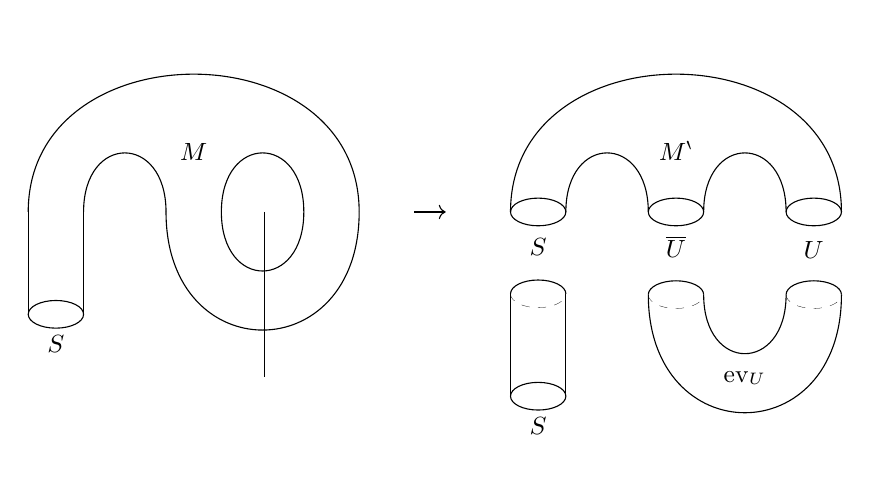
\begin{tikzpicture}[tqft/cobordism edge/.style={draw}]
  %left bottom 1
  \pic[tqft,name=mb,cobordism height=3cm,boundary separation=1.75cm,incoming boundary components=2,outgoing boundary components=0];

  %left top
  \pic[tqft,name=mt,cobordism height=3cm,boundary separation=1.75cm,incoming boundary components=0,outgoing boundary components=3,anchor=outgoing boundary 2,at=(mb-incoming boundary 1)];
  \node[at=(mt-outgoing boundary 2),above=15pt,font=\small]{$M$};

  %left bottom 2
  \pic[tqft/cylinder,name=cb,cobordism height=1.3cm,boundary separation=1.75cm,at=(mt-outgoing boundary 1),every outgoing boundary component/.style={draw}];
  \node[at=(cb-outgoing boundary 1),below=4pt,font=\small]{$S$};

  %cutting line
  \draw (0.9,0) -- (0.9,-2.1);

  %arrow
  \draw[->] (2.8,0) -- (3.2,0);

  %right top
  \pic[tqft,name=mp,cobordism height=3cm,boundary separation=1.75cm,incoming boundary components=0,outgoing boundary components=3,anchor={(-2.5,1)},at=(mt-outgoing boundary 1),every outgoing boundary component/.style={draw}];
  \node[at=(mp-outgoing boundary 2),above=15pt,font=\small]{$M^{\backprime}$};
  \node[at=(mp-outgoing boundary 1),below=6pt,font=\small]{$S$};
  \node[at=(mp-outgoing boundary 2),below=5pt,font=\small]{$\overline{U}$};
  \node[at=(mp-outgoing boundary 3),below=7pt,font=\small]{$U$};

  %right bottom
  \pic[tqft,name=ev,cobordism height=3cm,boundary separation=1.75cm,incoming boundary components=2,outgoing boundary components=0,anchor={(1,-0.35)},at=(mp-outgoing boundary 2),every incoming upper boundary component/.style={draw},every incoming lower boundary component/.style={draw,ultra thin,dashed}];
  \node[at=(ev-between incoming 1 and 2),below=1mm,font=\small]{$\mathrm{ev}_{U}$};
  \pic[tqft/cylinder,name=c,cobordism height=1.3cm,anchor={(1,-0.8)},at=(mp-outgoing boundary 1),every incoming upper boundary component/.style={draw},every incoming lower boundary component/.style={draw,ultra thin,dashed},every outgoing boundary component/.style={draw}];
  \node[at=(c-outgoing boundary 1),below=4pt,font=\small]{$S$};
\end{tikzpicture}
\caption{Cutting a cobordism along a closed submanifold}
\label{fig:cutopencob}
\end{figure}
Then
\begin{align*}
  Y([M])
  &=
  \mathsf{R}(Y(S))
  \circ
  \left(
    \mathrm{id}_{Y(S)}
    \otimes
    \mathrm{ev}_{Y(U)}
  \right)
  \circ
  \sim_{\mathsf{H}}
  \circ
  Y([M^{\backprime}])
\end{align*}
where
\begin{align*}
  \sim_{\mathsf{H}}
  \colon
  Y(S \sqcup (\overline{U} \sqcup U))
  &\to
  Y(S)
  \otimes
  (Y(\overline{U}) \otimes Y(U))
\end{align*}
is the obvious isomorphism built from $\mathsf{H}$
\newpage

\item[(AC3)]
for
\begin{align*}
  [M]
  \in
  \mathrm{mor}_{\mathbf{Cob}_{n}}(\emptyset,S)
  \qquad
  \text{and}
  \qquad
  [\tilde{M}]
  \in
  \mathrm{mor}_{\mathbf{Cob}_{n}}(\emptyset,\tilde{S})
\end{align*}
we have
\begin{align*}
  Y([M])
  \otimes
  Y(\tilde{[M]})
  &=
  \mathsf{H}(S,\tilde{S})^{-1}
  \circ
  Y([M] \sqcup [\tilde{M}])
  \circ
  \mathsf{H}(\emptyset,\emptyset)
\end{align*}

\item[(AC4),(AC5)]
$Y$ is compatible with the symmetric braidings, the associators and the unit laws of $\mathbf{Cob}_{n}$ and $\mathbf{Vec}_{K}$
\end{enumerate}
\end{enumerate}
If $Y$ satisfies the conditions in ii), then the extension to a symmetric monoidal functor in i) is unique.
\end{cor}
\begin{prf}
This follows from theorem \ref{THM:ACSMF} but for illustrative purposes we sketch the main idea here. The direction i) $\Rightarrow$ ii) is rather easy when using that monoidal functors preserve dual objects which we will show later. The idea for the other direction ii) $\Rightarrow$ i) is to extend $Y$ to all cobordisms by making a cobordism $M \colon S_{1} \to S_{2}$ into a cobordism with in-boundary $\emptyset$ using the coevaluation. More precisely, we can glue $M$ to one component of the cylinder representing $\mathrm{coev}_{S_{1}}$ to obtain
\begin{align*}
  M^{\backprime}
  \colon
  \emptyset
  &\to
  S_{2} \sqcup \overline{S}_{1}
\end{align*}
that is,
\begin{align*}
  [M^{\backprime}]
  &=
  ([M] \sqcup \mathrm{id}_{\overline{S}_{1}})
  \circ
  \mathrm{coev}_{S_{1}}
\end{align*}
See figure \ref{fig:cobto0in} for an illustration.
\\
\begin{figure}[h!]
\centering
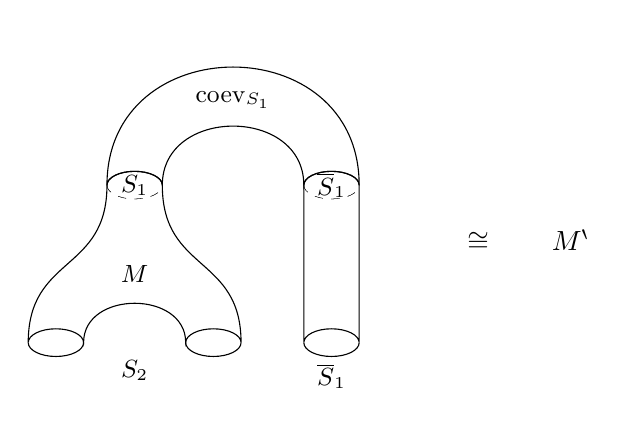
\begin{tikzpicture}[tqft/cobordism/.style={draw}]
  %top
  \pic[tqft,name=co,cobordism height=3cm,boundary separation=2.5cm,,incoming boundary components=0,outgoing boundary components=2,every outgoing lower boundary component/.style={draw,ultra thin,dashed}];
  \node[at=(co-outgoing boundary 2),below=-8pt,font=\small]{$\overline{S}_{1}$};
  \node[at=(co-between outgoing 1 and 2),above=3pt,font=\small]{$\mathrm{coev}_{S_{1}}$};
  
  %bottom
  \pic[tqft/pair of pants,name=p,at=(co-outgoing boundary 1),every incoming lower boundary component/.style={draw,ultra thin,dashed},every outgoing lower boundary component/.style={draw}];
  \node[at=(p-incoming boundary 1),font=\small]{$S_{1}$};
  \node[at=(p-between outgoing 1 and 2),above=4pt,font=\small]{$M$};
  \node[at=(p-between outgoing 1 and 2),below=6mm,font=\small]{$S_{2}$};
  \pic[tqft/cylinder,name=c,at=(co-outgoing boundary 2),every incoming lower boundary component/.style={draw,ultra thin,dashed},every outgoing lower boundary component/.style={draw}];
  \node[at=(c-outgoing boundary 1),below=4pt,font=\small]{$\overline{S}_{1}$};

  %right
  \node[at=(c-incoming boundary 1),below=7mm,right=1.6cm]{$\cong \qquad M^{\backprime}$};
\end{tikzpicture}
\caption{Turning the in-boundary of a cobordism into an out-boundary}
\label{fig:cobto0in}
\end{figure}
\\
Then we apply $Y$ to obtain a sort of copairing
\begin{align*}
  Y([M^{\backprime}])
  \colon
  K
  \cong
  Y(\emptyset)
  \to
  Y(S_{2} \sqcup \overline{S}_{1}) \cong Y(S_{2})
  \otimes
  Y(\overline{S}_{1})
\end{align*}
With the help of the pairing $\mathrm{ev}_{Y(S_{1})}$ we obtain a linear map from $Y(S_{1})$ to $Y(S_{2})$ by the composition
\begin{equation*}
\begin{tikzcd}[row sep=3em,column sep=8em]
  Y(S_{1})
  \ar{r}{Y([M^{\backprime}]) \otimes \mathrm{id}_{Y(S_{1})}}
  &
  Y(S_{2}) \otimes Y(\overline{S}_{1}) \otimes Y(S_{1})
  \ar{r}{\mathrm{id}_{Y(S_{2})} \otimes \mathrm{ev}_{Y(S_{1})}}
  &
  Y(S_{2})
\end{tikzcd}
\end{equation*}
where we suppressed the isomorphisms involved. If $Y$ is a functor, which we do not know yet, it is fairly easy to see that this coincides with $Y([M])$ so that the construction indeed makes sense. Now one has to check that $Y$ indeed is a symmetric monoidal functor but as we said above this follows from theorem \ref{THM:ACSMF}.
\\
\phantom{proven}
\hfill
$\Box$
\end{prf}
The details we glossed over will become clear later when we state and prove the more general assertion. But before doing so we give three lemmas concerning dual objects in a monoidal category. The first one is about the uniqueness of dual objects.
\\
\begin{lem}
\label{lem:dualunique}
Let
\begin{align*}
  \mathcal{M}_{\mathbf{C}}
  &=
  \left(
    \mathbf{C}
    ,
    \otimes
    ,
    \mathsf{A}
    ,
    1
    ,
    \mathsf{L}
    ,
    \mathsf{R}
  \right)
\end{align*}
be a monoidal category. If $X \in \mathrm{ob}_{\mathbf{C}}$ has a left (right) dual object then this dual object is unique up to a unique isomorphism.
\end{lem}
\begin{prf}
\begin{enumerate}
\item[(i)]
Let $X_{1}^{\prime},X_{2}^{\prime}$ be left dual objects of $X$ with evaluation and coevaluation
\begin{align*}
  e_{1}
  \colon
  X_{1}^{\prime}
  \otimes
  X
  &\to
  1
  ,\qquad
  c_{1}
  \colon
  1
  \to
  X
  \otimes
  X_{1}^{\prime}
\end{align*}
for $X_{1}^{\prime}$ and
\begin{align*}
  e_{2}
  \colon
  X_{2}^{\prime}
  \otimes
  X
  &\to
  1
  ,\qquad
  c_{2}
  \colon
  1
  \to
  X
  \otimes
  X_{2}^{\prime}
\end{align*}
for $X_{2}^{\prime}$. Define $f \in \mathrm{mor}_{\mathbf{C}}(X_{1}^{\prime},X_{2}^{\prime})$ and $g \in \mathrm{mor}_{\mathbf{C}}(X_{2}^{\prime},X_{1}^{\prime})$ such that the following two diagrams commute
\begin{equation*}
\begin{tikzcd}[row sep=2.8em,column sep=2.8em]
  &
  X_{1}^{\prime}
  \ar{r}{f}
  \ar{dl}[swap]{\mathsf{R}^{-1}(X_{1}^{\prime})}
  &
  X_{2}^{\prime}
  &
  \\
  X_{1}^{\prime} 1
  \ar{d}[swap]{\mathrm{id}_{X_{1}^{\prime}} \otimes c_{2}}
  &
  &
  &
  1 X_{2}^{\prime}
  \ar{lu}[swap]{\mathsf{L}(X_{2}^{\prime})}
  \\
  X_{1}^{\prime} (X X_{2}^{\prime})
  \ar{rrr}{\mathsf{A}^{-1}(X_{1}^{\prime},X,X_{2}^{\prime})}
  &
  &
  &
  (X_{1}^{\prime} X) X_{2}^{\prime}
  \ar{u}[swap]{e_{1} \otimes \mathrm{id}_{X_{2}^{\prime}}}
\end{tikzcd}
\end{equation*}
\begin{equation*}
\begin{tikzcd}[row sep=2.8em,column sep=2.8em]
  &
  X_{2}^{\prime}
  \ar{r}{g}
  \ar{dl}[swap]{\mathsf{R}^{-1}(X_{2}^{\prime})}
  &
  X_{1}^{\prime}
  &
  \\
  X_{2}^{\prime} 1
  \ar{d}[swap]{\mathrm{id}_{X_{2}^{\prime}} \otimes c_{1}}
  &
  &
  &
  1 X_{1}^{\prime}
  \ar{lu}[swap]{\mathsf{L}(X_{1}^{\prime})}
  \\
  X_{2}^{\prime} (X X_{1}^{\prime})
  \ar{rrr}{\mathsf{A}^{-1}(X_{2}^{\prime},X,X_{1}^{\prime})}
  &
  &
  &
  (X_{2}^{\prime} X) X_{1}^{\prime}
  \ar{u}[swap]{e_{2} \otimes \mathrm{id}_{X_{1}^{\prime}}}
\end{tikzcd}
\end{equation*}

\item[(ii)]
Now consider the following diagram
\begin{equation}
\label{dualuniquestrict}
\begin{tikzcd}[row sep=8em,column sep=9em]
  X_{1}^{\prime}
  \ar{r}{\mathrm{id}_{X_{1}^{\prime}} \otimes c_{1}}
  \ar{d}[swap]{\mathrm{id}_{X_{1}^{\prime}} \otimes c_{2}}
  \ar[bend right=50]{dd}{f}
  &
  X_{1}^{\prime} (X X_{1}^{\prime})
  \ar{rd}{\mathrm{id}_{X_{1}^{\prime} (X X_{1}^{\prime})}}
  \ar{d}[swap]{\mathrm{id}_{X_{1}^{\prime}} \otimes ((c_{2} \otimes \mathrm{id}_{X}) \otimes \mathrm{id}_{X_{1}^{\prime}})}
  &
  \\
  X_{1}^{\prime} (X X_{2}^{\prime})
  \ar{r}{\mathrm{id}_{X_{1}^{\prime}} \otimes (\mathrm{id}_{X X_{2}^{\prime}} \otimes c_{1})}
  \ar{d}[swap]{e_{1} \otimes \mathrm{id}_{X_{2}^{\prime}}}
  &
  X_{1}^{\prime} (((X X_{2}^{\prime}) X) X_{1}^{\prime})
  \ar{r}{\mathrm{id}_{X_{1}^{\prime}} \otimes ((\mathrm{id}_{X} \otimes e_{2}) \otimes \mathrm{id}_{X_{1}^{\prime}})}
  \ar{d}[swap]{(e_{1} \otimes \mathrm{id}_{X_{2}^{\prime} X}) \otimes \mathrm{id}_{X_{1}^{\prime}}}
  &
  X_{1}^{\prime} (X X_{1}^{\prime})
  \ar{d}{e_{1} \otimes \mathrm{id}_{X_{1}^{\prime}}}
  \\
  X_{2}^{\prime}
  \ar{r}{\mathrm{id}_{X_{2}^{\prime}} \otimes c_{1}}
  \ar[bend right]{rr}{g}
  &
  (X_{2}^{\prime} X) X_{1}^{\prime}
  \ar{r}{e_{2} \otimes \mathrm{id}_{X_{1}^{\prime}}}
  &
  X_{1}^{\prime}
\end{tikzcd}
\end{equation}
Here we suppressed the necessary isomorphisms $\mathsf{A}$, $\mathsf{L}$ and $\mathsf{R}$ for readability reasons, but it should be clear from what follows where they are needed. In the strict case, where $\mathsf{A}$, $\mathsf{L}$ and $\mathsf{R}$ are identities, the commutativity of the three small squares is immediate from the functoriality of the tensor product which ensures that\footnote{remember that we can insert unit objects wherever we want and can freely reparenthesize tensorings in the strict case}
\begin{align*}
  \left(
    \left(
      c_{2}
      \otimes
      \mathrm{id}_{X}
    \right)
    \otimes
    \mathrm{id}_{X_{1}^{\prime}}
  \right)
  \circ
  c_{1}
  &=
  \left(
    c_{2}
    \otimes
    \mathrm{id}_{X X_{1}^{\prime}}
  \right)
  \circ
  \left(
    \mathrm{id}_{1}
    \otimes
    c_{1}
  \right)
  \\
  &=
  c_{2}
  \otimes
  c_{1}
  \\
  &=
  \left(
    \mathrm{id}_{X X_{2}^{\prime}}
    \otimes
    c_{1}
  \right)
  \circ
  \left(
    c_{2}
    \otimes
    \mathrm{id}_{1}
  \right)
  \\
  &=
  \left(
    \mathrm{id}_{X X_{2}^{\prime}}
    \otimes
    c_{1}
  \right)
  \circ
  c_{2}
\end{align*}
in the upper left square. This suffices since by the functoriality of $\otimes$ we can add
\begin{align*}
  \mathrm{id}_{X_{1}^{\prime}}
  \otimes
\end{align*}
on the left of each morphism and still have an equality. The other squares can be shown analogously.
\\
In the non-strict case things are a bit more complicated, as we have to take care of the associators and unit laws. Yet the idea is still the same, of course, because the associators and unit laws are coherent so that they should not differ too much from identities. We exemplarily prove the commutativity of the upper left square, the other squares can be treated in a similar fashion. With all isomorphisms we have
\begin{equation*}
\begin{tikzcd}[row sep=4em,column sep=10em]
  X_{1}^{\prime}
  \ar{d}{\mathsf{R}^{-1}(X_{1}^{\prime})}
  &
  &
  \\
  X_{1}^{\prime} 1
  \ar{r}{\mathrm{id}_{X_{1}^{\prime}} \otimes c_{1}}
  \ar{d}[description]{\mathrm{id}_{X_{1}^{\prime}} \otimes c_{2}}
  &
  X_{1}^{\prime} (X X_{1}^{\prime})
  \ar{r}{\mathrm{id}_{X_{1}^{\prime}} \otimes (\mathsf{L}^{-1}(X)  \otimes  \mathrm{id}_{X_{1}^{\prime}})}
  &
  X_{1}^{\prime} ((1 X) X_{1}^{\prime})
  \ar{d}[description]{\mathrm{id}_{X_{1}^{\prime}} \otimes ((c_{2} \otimes \mathrm{id}_{X}) \otimes \mathrm{id}_{X_{1}^{\prime}})}
  \\
  X_{1}^{\prime} (X X_{2}^{\prime})
  \ar{d}[description]{\mathrm{id}_{X_{1}^{\prime}} \otimes \mathsf{R}^{-1}(X X_{2}^{\prime})}
  &
  &
  X_{1}^{\prime} (((X X_{2}^{\prime}) X) X_{1}^{\prime})
  \\
  X_{1}^{\prime} ((X X_{2}^{\prime}) 1)
  \ar{rr}{\mathrm{id}_{X_{1}^{\prime}} \otimes (\mathrm{id}_{X X_{2}^{\prime}} \otimes c_{1})}
  &
  &
  X_{1}^{\prime} ((X X_{2}^{\prime}) (X X_{1}^{\prime}))
  \ar{u}[description]{\mathrm{id}_{X_{1}^{\prime}} \otimes  \mathsf{A}^{-1}(X X_{2}^{\prime},X,X_{1}^{\prime})}
\end{tikzcd}
\end{equation*}
so, since $\mathsf{R}$ is an isomorphism, it suffices to show that the outer rectanlge of
\begin{equation*}
\begin{tikzcd}[row sep=4em,column sep=7em]
  1
  \ar{r}{c_{1}}
  \ar{rd}[swap]{\mathsf{R}^{-1}(1)}
  \ar{d}[swap]{c_{2}}
  &
  X X_{1}^{\prime}
  \ar{r}{\mathsf{L}^{-1}(X) \otimes \mathrm{id}_{X_{1}^{\prime}}}
  &
  (1 X) X_{1}^{\prime}
  \ar{d}{(c_{2} \otimes \mathrm{id}_{X}) \otimes \mathrm{id}_{X_{1}^{\prime}}}
  \\
  X X_{2}^{\prime}
  \ar{d}[swap]{\mathsf{R}^{-1}(X X_{2}^{\prime})}
  &
  11
  \ar{dl}[swap]{c_{2} \otimes \mathrm{id}_{1}}
  &
  ((X X_{2}^{\prime}) X) X_{1}^{\prime}
  \\
  (X X_{2}^{\prime}) 1
  \ar{rr}{\mathrm{id}_{X X_{2}^{\prime}} \otimes c_{1}}
  &
  &
  (X X_{2}^{\prime}) (X X_{1}^{\prime})
  \ar{u}[swap]{\mathsf{A}^{-1}(X X_{2}^{\prime},X,X_{1}^{\prime})}
\end{tikzcd}
\end{equation*}
commutes, where the left part commutes due to the naturality of $\mathsf{R}$. Using the identities
\begin{align*}
  \mathsf{L}(1)
  &=
  \mathsf{R}(1)
  \\
  \mathsf{L}^{-1}(X)
  \otimes
  \mathrm{id}_{X_{1}^{\prime}}
  &=
  \mathsf{A}^{-1}(1,X,X_{1}^{\prime})
  \circ
  \mathsf{L}^{-1}(X X_{1}^{\prime})
\end{align*}
which follow from the coherence theorem, we have to show for the right part that the outer rectangle of
\begin{equation*}
\begin{tikzcd}[row sep=4.2em,column sep=8.5em]
  1
  \ar{rr}{c_{1}}
  &
  &
  X X_{1}^{\prime}
  \ar{d}{\mathsf{L}^{-1}(X X_{1}^{\prime})}
  \\
  11
  \ar{r}{\mathrm{id}_{1} \otimes c_{1}}
  \ar{rd}[swap]{c_{2} \otimes c_{1}}
  \ar{u}{\mathsf{L}(1)}
  \ar{d}[swap]{c_{2} \otimes \mathrm{id}_{1}}
  &
  1 (X X_{1}^{\prime})
  \ar{r}{\mathrm{id}_{1 (X X_{1}^{\prime})}}
  \ar{ur}{\mathsf{L}(X X_{1}^{\prime})}
  &
  1 (X X_{1}^{\prime})
  \ar{d}{\mathsf{A}^{-1}(1,X,X_{1}^{\prime})}
  \ar{dl}{c_{2} \otimes \mathrm{id}_{X X_{1}^{\prime}}}
  \\
  (X X_{2}^{\prime}) 1
  \ar{d}[swap]{\mathrm{id}_{X X_{2}^{\prime}} \otimes c_{1}}
  &
  (X X_{2}^{\prime}) (X X_{1}^{\prime})
  \ar{rd}[xshift=-3mm,yshift=1mm]{\mathsf{A}^{-1}(X X_{2}^{\prime},X,X_{1}^{\prime})}
  \ar{dl}[swap,xshift=3mm,yshift=1mm]{\mathrm{id}_{(X X_{2}^{\prime}) (X X_{1}^{\prime})}}
  &
  (1 X) X_{1}^{\prime}
  \ar{d}{(c_{2} \otimes \mathrm{id}_{X}) \otimes \mathrm{id}_{X_{1}^{\prime}}}
  \\
  (X X_{2}^{\prime}) (X X_{1}^{\prime})
  \ar{rr}{\mathsf{A}^{-1}(X X_{2}^{\prime},X,X_{1}^{\prime})}
  &
  &
  ((X X_{2}^{\prime}) X) X_{1}^{\prime}
\end{tikzcd}
\end{equation*}
commutes. Here the upper left part is the naturality of $\mathsf{L}$, the lower right part is the naturality of $\mathsf{A}$ and the lower left and the central part are the functoriality of $\otimes$ which we already used in the strict case. The upper right and the lower triangle obviously commute, so that all inner diagrams commute. Hence so does the outer diagram.

\item[(iii)]
Back to diagram \eqref{dualuniquestrict}. The upper right triangle in diagram \eqref{dualuniquestrict} is just the first diagram (LD1) governing $e_{2},c_{2}$ with an $\mathrm{id}_{X_{1}^{\prime}}$ on the left and the right. Thus, the outer diagram commutes. The top right way of this outer diagram is $\mathrm{id}_{X_{1}^{\prime}}$ as follows from (LD2) for $e_{1},c_{1}$. But the left bottom way is just $g \circ f$, so we have shown
\begin{align*}
  g
  \circ
  f
  &=
  \mathrm{id}_{X_{1}^{\prime}}
\end{align*}
An analogous argument shows $f \circ g = \mathrm{id}_{X_{2}^{\prime}}$.

\item[(iv)]
As $f$ must be an isomorphism of dual objects we further have to show that
\begin{align*}
  c_{2}
  &=
  (\mathrm{id}_{X} \otimes f)
  \circ
  c_{1}
  ,\qquad
  e_{2}
  =
  e_{1}
  \circ
  (f^{-1} \otimes \mathrm{id}_{X})
\end{align*}
Again, in the strict case this is rather immediate by using the functoriality of the tensor product to change the positions of $c_{1}$ and the $c_{2}$ in $f$, and $e_{1}$ and the $e_{2}$ in $f^{-1} = g$, and subsequently applying the commuting diagrams governing $c_{1},e_{1}$. More precisely for the first equation we calculate
\begin{align*}
  (\mathrm{id}_{X} \otimes f)
  \circ
  c_{1}
  &=
  \left(
    \mathrm{id}_{X}
    \otimes
    \left(
      \left(
        e_{1}
        \otimes
        \mathrm{id}_{X_{2}^{\prime}}
      \right)
      \circ
      \left(
        \mathrm{id}_{X_{1}^{\prime}}
        \otimes
        c_{2}
      \right)
    \right)
  \right)
  \circ
  c_{1}
  \\
  &=
  \left(
    \mathrm{id}_{X}
    \otimes
    \left(
      e_{1}
      \otimes
      \mathrm{id}_{X_{2}^{\prime}}
    \right)
  \right)
  \circ
  \left(
    \mathrm{id}_{X X_{1}^{\prime}}
    \otimes
    c_{2}
  \right)
  \circ
  \left(
    c_{1}
    \otimes
    \mathrm{id}_{1}
  \right)
  \\
  &=
  \left(
    \left(
      \mathrm{id}_{X}
      \otimes
      e_{1}
    \right)
    \otimes
    \mathrm{id}_{X_{2}^{\prime}}
  \right)
  \circ
  \left(
    c_{1}
    \otimes
    \mathrm{id}_{X X_{2}^{\prime}}
  \right)
  \circ
  \left(
    \mathrm{id}_{1}
    \otimes
    c_{2}
  \right)
  \\
  &=
  \left(
    \left(
      \mathrm{id}_{X}
      \otimes
      e_{1}
    \right)
    \otimes
    \mathrm{id}_{X_{2}^{\prime}}
  \right)
  \circ
  \left(
    \left(
      c_{1}
      \otimes
      \mathrm{id}_{X}
    \right)
    \otimes
    \mathrm{id}_{X_{2}^{\prime}}
  \right)
  \circ
  c_{2}
  \\
  &=
  c_{2}
\end{align*}
In the last step we used (LD1) for $c_{1},e_{1}$. The second equation is treated similarly. The non-strict case again involves some tedious dealing with the coherence conditions. It is done similar as in step (ii) and we forgo it here.

\item[(v)]
For the uniqueness of the isomorphism let
\begin{align*}
  h
  \in
  \mathrm{mor}_{\mathbf{C}}(X_{1}^{\prime},X_{2}^{\prime})
\end{align*}
be another isomorphism for the duals, i.e.
\begin{align*}
  (\mathrm{id}_{X} \otimes f)
  \circ
  c_{1}
  &=
  c_{2}
  =
  (\mathrm{id}_{X} \otimes h)
  \circ
  c_{1}
  \\
  e_{1}
  \circ
  (f^{-1} \otimes \mathrm{id}_{X})
  &=
  e_{2}
  =
  e_{1}
  \circ
  (h^{-1} \otimes \mathrm{id}_{X})
\end{align*}
In the strict case we can easily calculate with the help of diagram (LD2) for $c_{1},e_{1}$ and $c_{2},e_{2}$ respectively, that
\begin{align*}
  h
  \circ
  f^{-1}
  &=
  \left(
    \mathrm{id}_{1}
    \otimes
    h
  \right)
  \circ
  \left(
    e_{1}
    \otimes
    \mathrm{id}_{X_{1}^{\prime}}
  \right)
  \circ
  \left(
    \mathrm{id}_{X_{1}^{\prime}}
    \otimes
    c_{1}
  \right)
  \circ
  \left(
    f^{-1}
    \otimes
    \mathrm{id}_{1}
  \right)
  \\
  &=
  \left(
    e_{1}
    \otimes
    \mathrm{id}_{X_{2}^{\prime}}
  \right)
  \circ
  \left(
    \left(
      \mathrm{id}_{X_{1}^{\prime}}
      \otimes
      \mathrm{id}_{X}
    \right)
    \otimes
    h
  \right)
  \circ
  \left(
    f^{-1}
    \otimes
    \left(
      \mathrm{id}_{X}
      \otimes
      \mathrm{id}_{X_{1}^{\prime}}
    \right)
  \right)
  \circ
  \left(
    \mathrm{id}_{X_{2}^{\prime}}
    \otimes
    c_{1}
  \right)
  \\
  &=
  \left(
    e_{1}
    \otimes
    \mathrm{id}_{X_{2}^{\prime}}
  \right)
  \circ
  \left(
    \left(
      f^{-1}
      \otimes
      \mathrm{id}_{X}
    \right)
    \otimes
    \mathrm{id}_{X_{2}^{\prime}}
  \right)
  \circ
  \left(
    \mathrm{id}_{X_{2}^{\prime}}
    \otimes
    \left(
      \mathrm{id}_{X}
      \otimes
      h
    \right)
  \right)
  \circ
  \left(
    \mathrm{id}_{X_{2}^{\prime}}
    \otimes
    c_{1}
  \right)
  \\
  &=
  \left(
    \left(
      e_{1}
      \circ
      \left(
        f^{-1}
        \otimes
        \mathrm{id}_{X}
      \right)
    \right)
    \otimes
    \mathrm{id}_{X_{2}^{\prime}}
  \right)
  \circ
  \left(
    \mathrm{id}_{X_{2}^{\prime}}
    \otimes
    \left(
      \left(
        \mathrm{id}_{X}
        \otimes
        h
      \right)
      \circ
      c_{1}
    \right)
  \right)
  \\
  &=
  \left(
    e_{2}
    \otimes
    \mathrm{id}_{X_{2}^{\prime}}
  \right)
  \circ
  \left(
    \mathrm{id}_{X_{2}^{\prime}}
    \otimes
    c_{2}
  \right)
  \\
  &=
  \mathrm{id}_{X_{2}^{\prime}}
\end{align*}
Hence we can conclude $h = f$. We forgo the non-strict case, as it is again just juggling with coherence conditions. Right duals can be treated in the same fashion.
\end{enumerate}
\phantom{proven}
\hfill
$\square$
\end{prf}
The second lemma basically states that monoidal functors preserve dual objects.
\\
\begin{lem}
\label{lem:mfduals}
Let $\mathbf{C},\mathbf{C}_{\alpha}$ be monoidal categories and let
\begin{align*}
  (F,\mathsf{H},\Phi)
  \colon
  \mathbf{C}
  \to
  \mathbf{C}_{\alpha}
\end{align*}
be a monoidal functor. Let $X \in \mathrm{ob}_{\mathbf{C}}$ have a left dual object $X^{\prime}$ with evaluation and coevaluation
\begin{align*}
  \mathrm{ev}_{X}
  \colon
  X^{\prime}
  \otimes
  X
  &\to
  1
  ,\qquad
  \mathrm{coev}_{X}
  \colon
  1
  \to
  X
  \otimes
  X^{\prime}
\end{align*}
Then $F(X^{\prime})$ is a left dual object of $F(X)$ with evaluation and coevaluation given by
\begin{align*}
  \mathrm{ev}_{F(X)}
  &:=
  \Phi^{-1}
  \circ
  F(\mathrm{ev}_{X})
  \circ
  \mathsf{H}(X^{\prime},X)
  \colon
  F(X^{\prime})
  \otimes_{\alpha}
  F(X)
  \to
  1_{\alpha}
  \\
  \mathrm{coev}_{F(X)}
  &:=
  \mathsf{H}^{-1}(X,X^{\prime})
  \circ
  F(\mathrm{coev}_{X})
  \circ
  \Phi
  \colon
  1_{\alpha}
  \to
  F(X)
  \otimes_{\alpha}
  F(X^{\prime})
\end{align*}
A similar result holds for right dual objects.
\end{lem}
\begin{prf}
Consider the commuting diagrams (LD1) and (LD2) governing the evaluation $\mathrm{ev}_{X}$ and coevaluation $\mathrm{coev}_{X}$ in $\mathbf{C}$,
\begin{equation*}
\begin{tikzcd}[row sep=3.2em,column sep=4.8em]
  1 X
  \ar{r}{\mathsf{L}(X)}
  \ar{d}[swap]{\mathrm{coev}_{X} \otimes \mathrm{id}_{X}}
  &
  X
  &
  X 1
  \ar{l}[swap]{\mathsf{R}(X)}
  \\
  (X X^{\prime}) X
  \ar{rr}{\mathsf{A}(X,X^{\prime},X)}
  &
  &
  X (X^{\prime} X)
  \ar{u}[swap]{\mathrm{id}_{X} \otimes \mathrm{ev}_{X}}
\end{tikzcd}
\end{equation*}
and
\begin{equation*}
\begin{tikzcd}[row sep=3.2em,column sep=4.8em]
  X^{\prime} 1
  \ar{r}{\mathsf{R}(X^{\prime})}
  \ar{d}[swap]{\mathrm{id}_{X^{\prime}} \otimes \mathrm{coev}_{X}}
  &
  X^{\prime}
  &
  1 X^{\prime}
  \ar{l}[swap]{\mathsf{L}(X^{\prime})}
  \\
  X^{\prime} (X X^{\prime})
  \ar{rr}{\mathsf{A}^{-1}(X^{\prime},X,X^{\prime})}
  &
  &
  (X^{\prime} X) X^{\prime}
  \ar{u}[swap]{\mathrm{ev}_{X} \otimes \mathrm{id}_{X^{\prime}}}
\end{tikzcd}
\end{equation*}
Applying $F$ to (LD1) yields
\begin{equation*}
\begin{tikzcd}[row sep=3.2em,column sep=4.8em]
  F(1 X)
  \ar{r}{F(\mathsf{L}(X))}
  \ar{d}[swap]{F(\mathrm{coev}_{X} \otimes \mathrm{id}_{X})}
  &
  F(X)
  &
  F(X 1)
  \ar{l}[swap]{F(\mathsf{R}(X))}
  \\
  F((X X^{\prime}) X)
  \ar{rr}{F(\mathsf{A}(X,X^{\prime},X))}
  &
  &
  F(X (X^{\prime} X))
  \ar{u}[swap]{F(\mathrm{id}_{X} \otimes \mathrm{ev}_{X})}
\end{tikzcd}
\end{equation*}
With the naturality of $\mathsf{H}$ we find
\begin{equation}
\label{mfdFdiag1}
\begin{tikzcd}[row sep=4.5em,column sep=3.8em,font=\footnotesize,every label/.append style={font=\tiny}]
  F(1) F(X)
  \ar{d}[description,xshift=2mm]{F(\mathrm{coev}_{X}) \otimes F(\mathrm{id}_{X})}
  &
  F(1 X)
  \ar{r}{F(\mathsf{L}(X))}
  \ar{d}[description,xshift=1mm]{F(\mathrm{coev}_{X} \otimes \mathrm{id}_{X})}
  \ar{l}[swap]{\mathsf{H}^{-1}(1,X)}
  &
  F(X)
  &
  F(X 1)
  \ar{l}[swap]{F(\mathsf{R}(X))}
  &
  F(X) F(1)
  \ar{l}[swap]{\mathsf{H}(X,1)}
  \\
  F(X X^{\prime}) F(X)
  \ar{r}{\mathsf{H}(X X^{\prime},X)}
  &
  F((X X^{\prime}) X)
  \ar{rr}{F(\mathsf{A}(X,X^{\prime},X))}
  &
  &
  F(X (X^{\prime} X))
  \ar{r}{\mathsf{H}^{-1}(X,X^{\prime} X)}
  \ar{u}[description,xshift=-1mm]{F(\mathrm{id}_{X} \otimes \mathrm{ev}_{X})}
  &
  F(X) F(X^{\prime} X)
  \ar{u}[description,xshift=-2mm]{F(\mathrm{id}_{X}) \otimes F(\mathrm{ev}_{X})}
\end{tikzcd}
\end{equation}
Now we use the compatilibity conditions for the associators and unit laws and $\mathsf{H}$ which can be expressed by the following commutative diagrams
\begin{equation*}
\begin{tikzcd}[row sep=3.2em,column sep=10em]
  (F(X) F(X^{\prime})) F(X)
  \ar{r}{\mathsf{A}_{\alpha}(F(X),F(X^{\prime}),F(X))}
  &
  F(X) (F(X^{\prime}) F(X))
  \ar{d}{\mathrm{id}_{F(X)} \otimes \mathsf{H}(X^{\prime},X)}
  \\
  F(X X^{\prime}) F(X)
  \ar{u}{\mathsf{H}^{-1}(X,X^{\prime}) \otimes \mathrm{id}_{F(X)}}
  \ar{d}[swap]{\mathsf{H}(X X^{\prime},X)}
  &
  F(X) F(X^{\prime} X)
  \\
  F((X X^{\prime}) X)
  \ar{r}{F(\mathsf{A}(X,X^{\prime},X))}
  &
  F(X (X^{\prime} X))
  \ar{u}[swap]{\mathsf{H}^{-1}(X,X^{\prime} X)}
\end{tikzcd}
\end{equation*}
\begin{equation*}
\begin{tikzcd}[row sep=3.2em,column sep=10em]
  F(X)
  \ar{r}{\mathsf{L}_{\alpha}^{-1}(F(X))}
  \ar{d}[swap]{F(\mathsf{L}^{-1}(X))}
  &
  1_{\alpha} F(X)
  \ar{d}{\Phi \otimes_{\alpha} \mathrm{id}_{F(X)}}
  \\
  F(1 X)
  \ar{r}{\mathsf{H}^{-1}(1,X)}
  &
  F(1) F(X)
\end{tikzcd}
\end{equation*}
\begin{equation*}
\begin{tikzcd}[row sep=3.2em,column sep=10em]
  F(X) F(1)
  \ar{r}{\mathrm{id}_{F(X)} \otimes_{\alpha} \Phi^{-1}}
  \ar{d}[swap]{\mathsf{H}(X,1)}
  &
  F(X) 1_{\alpha}
  \ar{d}{\mathsf{R}_{\alpha}(F(X))}
  \\
  F(X 1)
  \ar{r}{F(\mathsf{R}(X))}
  &
  F(X)
\end{tikzcd}
\end{equation*}
Using these relations in \eqref{mfdFdiag1} we obtain
\begin{equation*}
\begin{tikzcd}[row sep=4.5em,column sep=3.8em]
  1_{\alpha} F(X)
  \ar{r}{\mathsf{L}_{\alpha}(F(X))}
  \ar{d}[swap]{\Phi \otimes_{\alpha} \mathrm{id}_{F(X)}}
  &
  F(X)
  &
  F(X) 1_{\alpha}
  \ar{l}[swap]{\mathsf{R}_{\alpha}(F(X))}
  \\
  F(1) F(X)
  \ar{d}[swap]{F(\mathrm{coev}_{X}) \otimes \mathrm{id}_{F(X)}}
  &
  &
  F(X) F(1)
  \ar{u}[swap]{\mathrm{id}_{F(X)} \otimes_{\alpha} \Phi^{-1}}
  \\
  F(X X^{\prime}) F(X)
  \ar{d}[swap]{\mathsf{H}^{-1}(X,X^{\prime}) \otimes_{\alpha} \mathrm{id}_{F(X)}}
  &
  &
  F(X) F(X^{\prime} X)
  \ar{u}[swap]{\mathrm{id}_{F(X)} \otimes F(\mathrm{ev}_{X})}
  \\
  (F(X) F(X^{\prime})) F(X)
  \ar{rr}{\mathsf{A}_{\alpha}(F(X),F(X^{\prime}),F(X))}
  &
  &
  F(X) (F(X^{\prime}) F(X))
  \ar{u}[swap]{\mathrm{id}_{F(X)} \otimes_{\alpha} \mathsf{H}(X^{\prime},X)}
\end{tikzcd}
\end{equation*}
Now substituting the definitions of $\mathrm{coev}_{F(X)}$ and $\mathrm{ev}_{F(X)}$ we have exactly the first diagram (LD1) for dual objects
\begin{equation*}
\begin{tikzcd}[row sep=4.5em,column sep=4.2em]
  1_{\alpha} F(X)
  \ar{r}{\mathsf{L}_{\alpha}(F(X))}
  \ar{d}[swap]{\mathrm{coev}_{F(X)} \otimes_{\alpha} \mathrm{id}_{F(X)}}
  &
  F(X)
  &
  F(X) 1_{\alpha}
  \ar{l}[swap]{\mathsf{R}_{\alpha}(F(X))}
  \\
  (F(X) F(X^{\prime})) F(X)
  \ar{rr}{\mathsf{A}_{\alpha}(F(X),F(X^{\prime}),F(X))}
  &
  &
  F(X) (F(X^{\prime}) F(X))
  \ar{u}[swap]{\mathrm{id}_{F(X)} \otimes_{\alpha} \mathrm{ev}_{F(X)}}
\end{tikzcd}
\end{equation*}
In the same fashion we obtain (LD2) for $\mathrm{coev}_{F(X)}$ and $\mathrm{ev}_{F(X)}$ from (LD2) for $\mathrm{coev}_{X}$ and $\mathrm{ev}_{X}$. The proof for right dual objects works analogously.
\\
\phantom{proven}
\hfill
$\square$
\end{prf}
The third lemma is about tensoring dual objects. This statement is not very surprising when knowing the result about composition of pairs of adjoint functors and recognizing that basically duality is for objects what adjointness is for functors. The latter will become clearer in part \ref{part:higher} where full dualizability and the delooping hypothesis are treated.
\\
\begin{lem}
\label{LEM:DUALOBTENSOR}
Let $\mathbf{C}$ be a monoidal category and let $X_{1},X_{2} \in \mathrm{ob}_{\mathbf{C}}$ have left dual objects $X_{1}^{\prime},X_{2}^{\prime}$ with coevaluations $\mathrm{coev}_{X_{1}},\mathrm{coev}_{X_{2}}$ and evaluations $\mathrm{ev}_{X_{1}},\mathrm{ev}_{X_{2}}$, respectively. Then $X_{2}^{\prime} \otimes X_{1}^{\prime}$ is a left dual object of $X_{1} \otimes X_{2}$ where the coevaluation is given by
\begin{equation*}
\begin{tikzcd}[row sep=3.2em,column sep=8em]
  1
  \ar{rr}{\mathrm{coev}_{X_{1} X_{2}}}
  \ar{d}[swap]{\mathrm{coev}_{X_{1}}}
  &
  &
  (X_{1} X_{2}) (X_{2}^{\prime} X_{1}^{\prime})
  \\
  X_{1} X_{1}^{\prime}
  \ar{r}{\mathsf{R}^{-1}(X_{1}) \otimes \mathrm{id}_{X_{1}^{\prime}}}
  &
  (X_{1} 1) X_{1}^{\prime}
  \ar{r}{(\mathrm{id}_{X_{1}} \otimes \mathrm{coev}_{X_{2}}) \otimes \mathrm{id}_{X_{1}^{\prime}}}
  &
  (X_{1} (X_{2} X_{2}^{\prime})) X_{1}^{\prime}
  \ar{u}[swap]{i_{\mathsf{A}}^{(c)}}
\end{tikzcd}
\end{equation*}
and the evaluation is given by
\begin{equation*}
\begin{tikzcd}[row sep=3.2em,column sep=8em]
  (X_{2}^{\prime} X_{1}^{\prime}) (X_{1} X_{2})
  \ar{rr}{\mathrm{ev}_{X_{1} X_{2}}}
  \ar{d}[swap]{i_{\mathsf{A}}^{(e)}}
  &
  &
  1
  \\
  X_{2}^{\prime} ((X_{1}^{\prime} X_{1}) X_{2})
  \ar{r}{\mathrm{id}_{X_{2}^{\prime}} \otimes (\mathrm{ev}_{X_{1}} \otimes \mathrm{id}_{X_{2}})}
  &
  X_{2}^{\prime} (1 X_{2})
  \ar{r}{\mathrm{id}_{X_{2}^{\prime}} \otimes \mathsf{L}(X_{2})}
  &
  X_{2}^{\prime} X_{2}
  \ar{u}[swap]{\mathrm{ev}_{X_{2}}}
\end{tikzcd}
\end{equation*}
with $i_{\mathsf{A}}^{(c)}$ and $i_{\mathsf{A}}^{(e)}$ the corresponding unique\footnote{the uniqueness is guaranteed by the coherence theorem} isomorphisms built from the associator.
\\
In the case of a symmetric monoidal category the coevaluation and the evaluation can be written as
\begin{equation*}
\begin{tikzcd}[row sep=3.2em,column sep=8em]
  1
  \ar{r}{\mathrm{coev}_{X_{1} X_{2}}}
  \ar{d}[swap]{\mathsf{R}^{-1}(1)}
  &
  (X_{1} X_{2}) (X_{2}^{\prime} X_{1}^{\prime})
  \\
  1 1
  \ar{r}{\mathrm{coev}_{X_{1}} \otimes \mathrm{coev}_{X_{2}}}
  &
  (X_{1} X_{1}^{\prime}) (X_{2} X_{2}^{\prime})
  \ar{u}[swap]{i^{(c)}}
\end{tikzcd}
\end{equation*}
and
\begin{equation*}
\begin{tikzcd}[row sep=3.2em,column sep=8em]
  (X_{2}^{\prime} X_{1}^{\prime}) (X_{1} X_{2})
  \ar{r}{\mathrm{ev}_{X_{1} X_{2}}}
  \ar{d}[swap]{i^{(e)}}
  &
  1
  \\
  (X_{1}^{\prime} X_{1}) (X_{2}^{\prime} X_{2})
  \ar{r}{\mathrm{ev}_{X_{1}} \otimes \mathrm{ev}_{X_{2}}}
  &
  1 1
  \ar{u}[swap]{\mathsf{L}(1)}
\end{tikzcd}
\end{equation*}
where $i^{(c)}$ and $i^{(e)}$ are the corresponding unique isomorphisms built from the associator and the braiding.
\end{lem}
\begin{prf}[Sketch]
We only sketch the proof for a strict monoidal category\footnote{again, remember that we can insert unit objects wherever we want and do not have to care about parentheses in the strict case} and give a more detailed proof in the appendix.
\\
\newpage
From the definitions we find that the outer perimeter of the following diagram commutes. The lower left part commutes because of the functoriality of the tensor product.
\begin{equation*}
\hspace{-2em}
\begin{tikzcd}[row sep=7em,column sep=6em]
  1 X_{1} X_{2}
  \ar{rr}{\mathrm{coev}_{X_{1} X_{2}} \otimes \mathrm{id}_{X_{1} X_{2}}}
  \ar{d}[swap]{\mathrm{coev}_{X_{1}} \otimes \mathrm{id}_{X_{1}} \otimes \mathrm{id}_{X_{2}}}
  &
  &
  X_{1} X_{2} X_{2}^{\prime} X_{1}^{\prime} X_{1} X_{2}
  \ar{d}{\mathrm{id}_{X_{1} X_{2}} \otimes \mathrm{ev}_{X_{1} X_{2}}}
  \\
  X_{1} X_{1}^{\prime} X_{1} X_{2}
  \ar{r}{\mathrm{id}_{X_{1}} \otimes (\mathrm{ev}_{X_{1}} \otimes \mathrm{id}_{X_{2}})}
  \ar{d}[swap]{(\mathrm{id}_{X_{1}} \otimes \mathrm{coev}_{X_{2}}) \otimes \mathrm{id}_{X_{1}^{\prime} X_{1} X_{2}}}
  &
  X_{1} 1 X_{2}
  \ar{rd}[description]{(\mathrm{id}_{X_{1}} \otimes \mathrm{coev}_{X_{2}}) \otimes \mathrm{id}_{X_{2}}}
  &
  X_{1} X_{2} 1
  \\
  X_{1} X_{2} X_{2}^{\prime} X_{1}^{\prime} X_{1} X_{2}
  \ar{rr}{\mathrm{id}_{X_{1} X_{2} X_{2}^{\prime}} \otimes (\mathrm{ev}_{X_{1}} \otimes \mathrm{id}_{X_{2}})}
  &
  &
  X_{1} X_{2} X_{2}^{\prime} X_{2}
  \ar{u}[swap]{\mathrm{id}_{X_{1}} \otimes \mathrm{id}_{X_{2}} \otimes \mathrm{ev}_{X_{2}}}
\end{tikzcd}
\end{equation*}
Going the inner way yields the following outer diagram. The inner parts on the left and lower right are diagram (LD1) governing dual objects for $X_{1}, X_{1}^{\prime}$ and $X_{2}, X_{2}^{\prime}$ respectively. The central part obviously commutes.
\begin{equation*}
\hspace{-2em}
\begin{tikzcd}[row sep=7em,column sep=6em]
  1 X_{1} X_{2}
  \ar{rr}{\mathrm{coev}_{X_{1} X_{2}} \otimes \mathrm{id}_{X_{1} X_{2}}}
  \ar{rrd}[description]{\mathrm{id}_{X_{1} X_{2}}}
  \ar[bend left=60]{dd}[description,xshift=1mm]{\mathrm{id}_{X_{1}} \otimes \mathrm{id}_{X_{2}}}
  \ar{d}[swap]{\mathrm{coev}_{X_{1}} \otimes \mathrm{id}_{X_{1}} \otimes \mathrm{id}_{X_{2}}}
  &
  &
  X_{1} X_{2} X_{2}^{\prime} X_{1}^{\prime} X_{1} X_{2}
  \ar{d}{\mathrm{id}_{X_{1} X_{2}} \otimes \mathrm{ev}_{X_{1} X_{2}}}
  \\
  X_{1} X_{1}^{\prime} X_{1} X_{2}
  \ar{d}[swap]{\mathrm{id}_{X_{1}} \otimes \mathrm{ev}_{X_{1}} \otimes \mathrm{id}_{X_{2}}}
  &
  &
  X_{1} X_{2} 1
  \\
  X_{1} 1 X_{2}
  \ar{urr}[description]{\mathrm{id}_{X_{1}} \otimes \mathrm{id}_{X_{2}}}
  \ar{rr}{\mathrm{id}_{X_{1}} \otimes \mathrm{coev}_{X_{2}} \otimes \mathrm{id}_{X_{2}}}
  &
  &
  X_{1} X_{2} X_{2}^{\prime} X_{2}
  \ar{u}[swap]{\mathrm{id}_{X_{1}} \otimes \mathrm{id}_{X_{2}} \otimes \mathrm{ev}_{X_{2}}}
\end{tikzcd}
\end{equation*}
But the upper right part is precisely the first diagram (LD1) governing dual objects for $X_{1} \otimes X_{2}$ and $X_{2}^{\prime} \otimes X_{1}^{\prime}$. The commutativity of the second diagram (LD2) can be shown in the same way.
\\
\phantom{proven}
\hfill
$\Box$
\end{prf}
Now we come to the more general statement about a characterization of a symmetric monoidal functor. We will be more precise here and the details we glossed over at the beginning of this section where we characterized a TQFT will become clear.
\\
\begin{thm}
\label{THM:ACSMF}
Let $\mathbf{C}$, $\mathbf{C}_{\alpha}$ be symmetric monoidal categories and let $\mathbf{C}$ be left\footnote{the category is also a right rigid then since it is braided} rigid. Let $E$ be a tuple $(E_{\mathrm{ob}},E_{\mathrm{mor}},\mathsf{H},\Phi)$ of
\begin{enumerate}
\item
a function
\begin{align*}
  E_{\mathrm{ob}}
  \colon
  \mathrm{ob}_{\mathbf{C}}
  &\to
  \mathrm{ob}_{\mathbf{C}_{\alpha}}
\end{align*}

\item
a function $E_{\mathrm{mor}}$ which maps $X \in \mathrm{ob}_{\mathbf{C}}$ to a function
\begin{align*}
  E_{\mathrm{mor}}(X)
  \colon
  \mathrm{mor}_{\mathbf{C}}(1,X)
  &\to
  \mathrm{mor}_{\mathbf{C}_{\alpha}}
  \left(
    E_{\mathrm{ob}}(1)
    ,
    E_{\mathrm{ob}}(X)
  \right)
\end{align*}

\item
a function $\mathsf{H}$ assigning to each object
\begin{align*}
  (X_{1},X_{2})
  \in
  \mathrm{ob}_{\mathbf{C} \times \mathbf{C}}
\end{align*}
an isomorphism
\begin{align*}
  \mathsf{H}(X_{1},X_{2})
  \in
  \mathrm{mor}_{\mathbf{C}_{\alpha}}
  \left(
    E_{\mathrm{ob}}(X_{1})
    \otimes_{\alpha}
    E_{\mathrm{ob}}(X_{2})
    ,
    E_{\mathrm{ob}}(X_{1} \otimes X_{2})
  \right)
\end{align*}

\item
an isomorphism
\begin{align*}
  \Phi
  \in
  \mathrm{mor}_{\mathbf{C}_{\alpha}}
  \left(
    1_{\alpha}
    ,
    E_{\mathrm{ob}}(1)
  \right)
\end{align*}
\end{enumerate}
In abuse of notation we will simply write $E$ for both $E_{\mathrm{ob}}$ and all $E_{\mathrm{mor}}(X)$. Then the following are equivalent
\begin{enumerate}
\item[i)]
$E$ extends to a symmetric monoidal functor from $\mathbf{C}$ to $\mathbf{C}_{\alpha}$

\item[ii)]
$E$ satisfies
\begin{enumerate}
\item[(AC1)]
for each $X \in \mathrm{ob}_{\mathbf{C}}$ and left dual object $X^{\prime}$ with evaluation $\mathrm{ev}_{X}$ and coevaluaton $\mathrm{coev}_{X}$ there is a morphism
\begin{align*}
  \mathrm{ev}_{E(X)}
  \in
  \mathrm{mor}_{\mathrm{C}_{\alpha}}
  \left(
    E(X^{\prime})
    \otimes_{\alpha}
    E(X)
    ,
    1_{\alpha}
  \right)
\end{align*}
which makes $E(X^{\prime})$ a left dual object of $E(X)$ with coevaluation map
\begin{align*}
  \mathrm{coev}_{E(X)}
  &:=
  \mathsf{H}(X,X^{\prime})^{-1}
  \circ
  E(\mathrm{coev}_{X})
  \circ
  \Phi
\end{align*}
Remember that this means that the following diagrams commute
\begin{equation*}
\begin{tikzcd}[row sep=3.3em,column sep=4.5em]
  1_{\alpha} E(X)
  \ar{r}{\mathsf{L}_{\alpha}(E(X))}
  \ar{d}[swap]{\mathrm{coev}_{E(X)} \otimes_{\alpha} \mathrm{id}_{E(X)}}
  &
  E(X)
  &
  E(X) 1_{\alpha}
  \ar{l}[swap]{\mathsf{R}_{\alpha}(E(X))}
  \\
  (E(X) E(X^{\prime})) E(X)
  \ar{rr}{\mathsf{A}_{\alpha}(E(X),E(X^{\prime}),E(X))}
  &
  &
  E(X) (E(X^{\prime}) E(X))
  \ar{u}[swap]{\mathrm{id}_{E(X)} \otimes_{\alpha} \mathrm{ev}_{E(X)}}
\end{tikzcd}
\end{equation*}
\begin{equation*}
\begin{tikzcd}[row sep=3.3em,column sep=4.5em]
  E(X^{\prime}) 1_{\alpha}
  \ar{r}{\mathsf{R}_{\alpha}(E(X^{\prime}))}
  \ar{d}[swap]{\mathrm{id}_{E(X^{\prime})} \otimes_{\alpha} \mathrm{coev}_{E(X)}}
  &
  E(X^{\prime})
  &
  1_{\alpha} E(X^{\prime})
  \ar{l}[swap]{\mathsf{L}_{\alpha}(E(X^{\prime}))}
  \\
  E(X^{\prime}) (E(X) E(X^{\prime}))
  \ar{rr}{\mathsf{A}_{\alpha}^{-1}(E(X^{\prime}),E(X),E(X^{\prime}))}
  &
  &
  (E(X^{\prime}) E(X)) E(X^{\prime})
  \ar{u}[swap]{\mathrm{ev}_{E(X)} \otimes_{\alpha} \mathrm{id}_{E(X^{\prime})}}
\end{tikzcd}
\end{equation*}

\item[(AC2)]
for all $X_{1},X_{2} \in \mathrm{ob}_{\mathbf{C}}$, left dual objects $X_{1}^{\prime}$ of $X_{1}$ and all
\begin{align*}
  f
  \in
  \mathrm{mor}_{\mathbf{C}}
  \left(
    1
    ,
    X_{2}
    \otimes
    (X_{1}^{\prime} \otimes X_{1})
  \right)
\end{align*}
the following diagram commutes
\begin{equation*}
\hspace{1cm}
\begin{tikzcd}[row sep=3.3em,column sep=7.5em]
  E(1)
  \ar{r}{E(\mathsf{R}(X_{2}) \circ (\mathrm{id}_{X_{2}} \otimes \mathrm{ev}_{X_{1}}) \circ f)}
  \ar{d}[swap]{E(f)}
  &
  E(X_{2})
  &
  E(X_{2}) 1_{\alpha}
  \ar{l}[swap]{\mathsf{R}_{\alpha}(E(X_{2}))}
  \\
  E(X_{2} (X_{1}^{\prime} X_{1}))
  \ar{r}{\mathsf{H}(X_{2},X_{1}^{\prime} X_{1})^{-1}}
  &
  E(X_{2}) (E(X_{1}^{\prime} X_{1}))
  \ar{r}{\mathrm{id}_{E(X_{2})} \otimes_{\alpha} \mathsf{H}(X_{1}^{\prime},X_{1})^{-1}}
  &
  E(X_{2}) (E(X_{1}^{\prime}) E(X_{1}))
  \ar{u}[swap]{\mathrm{id}_{E(X_{2})} \otimes_{\alpha} \mathrm{ev}_{E(X_{1})}}
\end{tikzcd}
\end{equation*}

\item[(AC3)]
for all
\begin{align*}
  f_{1}
  \in
  \mathrm{mor}_{\mathbf{C}}(1,X_{1})
  ,\qquad
  f_{2}
  \in
  \mathrm{mor}_{\mathbf{C}}(1,X_{2})
\end{align*}
the following diagram commutes
\begin{equation*}
\begin{tikzcd}[row sep=3.3em,column sep=8em]
  E(1)
  \ar{r}{E((f_{1} \otimes f_{2}) \circ \mathsf{L}^{-1}(1))}
  \ar{d}[swap]{\mathsf{L}_{\alpha}^{-1}(E(1))}
  &
  E(X_{1} X_{2})
  \\
  1_{\alpha} E(1)
  \ar{d}[swap]{\Phi \otimes_{\alpha} \mathrm{id}_{E(1)}}
  &
  \\
  E(1) E(1)
  \ar{r}{E(f_{1}) \otimes_{\alpha} E(f_{2})}
  &
  E(X_{1}) E(X_{2})
  \ar{uu}[swap]{\mathsf{H}(X_{1},X_{2})}
\end{tikzcd}
\end{equation*}

\item[(AC4)]
let
\begin{align*}
  X_{1}
  ,
  \ldots
  ,
  X_{n}
  \in
  \mathrm{ob}_{\mathbf{C}}
  ,\qquad
  n
  \in
  \mathbb{N}^{\times}
\end{align*}
and let $W$ be the tensor product of $X_{1},\dots,X_{n}$ in this order, with any choice of bracketing. Let $\pi \in S_{n}$ be a permutation and write $W_{\pi}$ for the tensor product of $X_{\pi(1)},\dots,X_{\pi(n)}$ in this order and with any choice of bracketing which may be different from that of $W$. There is an isomorphism
\begin{align*}
    \hat{\pi}
    \colon
    W
    &\to
    W_{\pi}
\end{align*}
built from the symmetric braiding $\mathsf{B}$ and the associator $\mathsf{A}$. This isomorphism is unique since though it can possibly be written in many ways, the coherence theorem ensures that these ways are all equal. Furthermore, let $W^{E}$ be the tensor product of $E(X_{1}),\dots,E(X_{n})$ in this order, with the same bracketing as $W$ and likewise for $W_{\pi}^{E}$ and $E(X_{\pi(1)}),\dots,E(X_{\pi(n)})$. We denote the corresponding unique isomorphism by
\begin{align*}
  \hat{\pi}_{\alpha}
  \colon
  W^{E}
  &\to
  W_{\pi}^{E}
\end{align*}
Additionally, we write
\begin{align*}
  \mathsf{H}^{W}
  \colon
  W^{E}
  &\to
  E(W)
\end{align*}
for the isomorphism obtained by subsequent applicaton of $\mathsf{H}$ (tensored with appropriate identities) and analogously for
\begin{align*}
  \mathsf{H}_{\pi}^{W}
  \colon
  W_{\pi}^{E}
  &\to
  E(W_{\pi})
\end{align*}
Then for $f \in \mathrm{mor}_{\mathbf{C}}(1,W)$ the following diagram commutes
\begin{equation*}
\begin{tikzcd}[row sep=3.3em,column sep=large]
  E(1)
  \ar{rr}{E(\hat{\pi} \circ f)}
  \ar{d}[swap]{E(f)}
  &
  &
  E(W_{\pi})
  \\
  E(W)
  \ar{r}{\mathsf{H}^{W -1}}
  &
  W^{E}
  \ar{r}{\hat{\pi}_{\alpha}}
  &
  W_{\pi}^{E}
  \ar{u}[swap]{\mathsf{H}_{\pi}^{W}}
\end{tikzcd}
\end{equation*}

\item[(AC5)]
for the unit object the equation
\begin{align*}
  E(\mathrm{id}_{1})
  &=
  \mathrm{id}_{E(1)}
\end{align*}
holds and the following diagrams commute
\begin{equation*}
\begin{tikzcd}[row sep=3.3em,column sep=4em]
  1_{\alpha} E(1)
  \ar{r}{\mathsf{L}_{\alpha}(E(1))}
  \ar{d}[swap]{\Phi \otimes_{\alpha} \mathrm{id}_{E(1)}}
  &
  E(1)
  \\
  E(1) E(1)
  \ar{r}{\mathsf{H}(1,1)}
  &
  E(1 1)
  \ar{u}[swap]{E(\mathsf{L}(1))}
\end{tikzcd}
\qquad
\begin{tikzcd}[row sep=3.3em,column sep=4em]
  E(1) 1_{\alpha}
  \ar{r}{\mathsf{R}_{\alpha}(E(1))}
  \ar{d}[swap]{\mathrm{id}_{E(1)} \otimes_{\alpha} \Phi}
  &
  E(1)
  \\
  E(1) E(1)
  \ar{r}{\mathsf{H}(1,1)}
  &
  E(1 1)
  \ar{u}[swap]{E(\mathsf{R}(1))}
\end{tikzcd}
\end{equation*}
\end{enumerate}
\end{enumerate}
The extension to a symmetric monoidal functor in i) is unique if $E$ satisfies the conditions in ii).
\end{thm}
\begin{prf}[Sketch]
The proof is not too difficult but quite tedious and lengthy as it involves a lot of dealing with the associators, unit laws and braidings and the diagrams in (AC1) - (AC5). Therefore we only give a sketch of how to proceed and refer to the appendix for all the (not very insightful) details.
\\\\
i) $\Rightarrow$ ii)
\qquad
This direction is rather immediate. We denote the symmetric monoidal functor which is an extension of $(E,\mathsf{H},\Phi)$ by $(F,\mathsf{H},\Phi)$ and define the evaluation for $E(X^{\prime})$ to be
\begin{align*}
  \mathrm{ev}_{E(X)}
  &:=
  \Phi^{-1}
  \circ
  F(\mathrm{ev}_{X})
  \circ
  \mathsf{H}(X^{\prime},X)
  \colon
  F(X^{\prime})
  \otimes_{\alpha}
  F(X)
  \to
  1_{\alpha}
\end{align*}
The diagrams in (AC1) are just lemma \ref{lem:mfduals}. We leave the rest out as the other conditions can be checked fairly easily: for (AC2) and (AC3) one uses the functoriality of $F$, (MF2) and the naturality of $\mathsf{H}$; (AC4) follows by the functoriality of $F$ and multiple application of (MF1) and (BF); (AC5) is just the functoriality of $F$ and a special case of (MF2).
\\\\
ii) $\Rightarrow$ i)
\qquad
This part is a rather long story. Set $F_{\mathrm{ob}} := E_{\mathrm{ob}}$. We have to extend $E$ to all morphisms in $\mathbf{C}$. To this end we need a left dual object $X^{\prime}$ for every object $X \in \mathrm{ob}_{\mathbf{C}}$. We know that $\mathbf{C}$ is left rigid, so these dual objects exist and we can suppose that there is a choice function to choose them or that they have been constructed explicitly. Either way, we choose $1^{\prime} = 1$ with
\begin{align*}
  \mathrm{coev}_{1}
  &=
  \mathsf{L}^{-1}(1)
  =
  \mathsf{R}^{-1}(1)
  \\
  \mathrm{ev}_{1}
  &=
  \mathsf{L}(1)
  =
  \mathsf{R}(1)
\end{align*}
and for tensor products we take dual objects as given by lemma \ref{LEM:DUALOBTENSOR}. Now for
\begin{align*}
  f_{12}
  \in
  \mathrm{mor}_{\mathbf{C}}(X_{1},X_{2})
\end{align*}
define
\begin{align*}
  \tilde{f}_{12}
  &:=
  \left(
    f_{12}
    \otimes
    \mathrm{id}_{X_{1}^{\prime}}
  \right)
  \circ
  \mathrm{coev}_{X_{1}}
  \colon
  1
  \to
  X_{2}
  \otimes
  X_{1}^{\prime}
  \\
  \gamma_{f_{12}}
  &:=
  \mathsf{H}(X_{2},X_{1}^{\prime})^{-1}
  \circ
  E(\tilde{f}_{12})
  \circ
  \Phi
  \colon
  1_{\alpha}
  \to
  E(X_{2})
  \otimes
  E(X_{1}^{\prime})
\end{align*}
Then we let $F_{\mathrm{mor}}$ be the function that maps
\begin{align*}
  (X_{1},X_{2})
  \in
  \mathrm{ob}_{\mathbf{C}}
  \times
  \mathrm{ob}_{\mathbf{C}}
\end{align*}
to the function
\begin{align*}
  F_{\mathrm{mor}}(X_{1},X_{2})
  \colon
  \mathrm{mor}_{\mathbf{C}}(X_{1},X_{2})
  &\to
  \mathrm{mor}_{\mathbf{C}_{\alpha}}(F_{\mathrm{ob}}(X_{1}),F_{\mathrm{ob}}(X_{2}))
\end{align*}
defined by the following commuting diagram
\begin{equation*}
\begin{tikzcd}[row sep=3.2em,column sep=10em]
  E(X_{1})
  \ar{r}{F_{\mathrm{mor}}(X_{1},X_{2})(f_{12})}
  \ar{d}[swap]{\mathsf{L}_{\alpha}^{-1}(E(X_{1}))}
  &
  E(X_{2})
  \\
  1_{\alpha} E(X_{1})
  \ar{d}[swap]{\gamma_{f_{12}} \otimes_{\alpha} \mathrm{id}_{E(X_{1})}}
  &
  E(X_{2}) 1_{\alpha}
  \ar{u}[swap]{\mathsf{R}_{\alpha}(E(X_{2}))}
  \\
  (E(X_{2}) E(X_{1}^{\prime})) E(X_{1})
  \ar{r}{\mathsf{A}_{\alpha}(E(X_{2}),E(X_{1}^{\prime}),E(X_{1}))}
  &
  E(X_{2}) (E(X_{1}^{\prime}) E(X_{1}))
  \ar{u}[swap]{\mathrm{id}_{E(X_{2})} \otimes_{\alpha} \mathrm{ev}_{E(X_{1})}}
\end{tikzcd}
\end{equation*}
Again we will write $F$ for both $F_{\mathrm{ob}}$ and all $F_{\mathrm{mor}}(X_{1},X_{2})$.
\\\\
We need to check that $F$ actually extends $E$, i.e. that for $g \in \mathrm{mor}_{\mathbf{C}}(1,Y)$ we have
\begin{align*}
  F(g)
  &=
  E(g)
\end{align*}
Using that $1^{\prime} = 1$ it is easy to see with the help of (AC3) and $E(\mathrm{id}_{1}) = \mathrm{id}_{E(1)}$ from (AC5) that
\begin{align*}
  \gamma_{g}
  &=
  \left(
    E(g)
    \otimes_{\alpha}
    \mathrm{id}_{E(1)}
  \right)
  \circ
  \mathrm{coev}_{E(1)}
\end{align*}
Substituting this in the definition of $F(g)$ and using (AC1) one can obtain the wanted result.
\\\\
Next, we have to verify that $(F,\mathsf{H},\Phi)$ is a symmetric monoidal functor from $\mathbf{C}$ to $\mathbf{C}_{\alpha}$. We verify the properties step by step.
\begin{enumerate}
\item[(F1)]
\begin{align*}
  \mathrm{F}(\mathrm{id}_{X})
  &=
  \mathrm{id}_{F(X)}
\end{align*}
follows immediately from (AC1) since
\begin{align*}
  \widetilde{\mathrm{id}}_{X}
  &=
  \mathrm{coev}_{X}
\end{align*}
implying that
\begin{align*}
  \gamma_{\mathrm{id}_{X}}
  &=
  \mathsf{H}(X,X^{\prime})^{-1}
  \circ
  E(\mathrm{coev}_{X})
  \circ
  \Phi
  \\
  &=
  \mathrm{coev}_{E(X)}
\end{align*}

\item[(F2)]
\begin{align*}
  F(f_{23} \circ f_{12})
  &=
  F(f_{23}) \circ F(f_{12})
\end{align*}
for
\begin{align*}
  f_{12} \in \mathrm{mor}_{\mathbf{C}}(X_{1},X_{2})
  ,\qquad
  f_{23} \in \mathrm{mor}_{\mathbf{C}}(X_{2},X_{3})
\end{align*}
needs a rather lengthy calculation. To further ease notation we define
\begin{align*}
  E_{i}
  &:=
  E(X_{i})
  ,\qquad
  E_{i}^{\prime}
  :=
  E(X_{i}^{\prime})
  ,\qquad
  1
  \leq
  i
  \leq
  4
\end{align*}
By definition we have the following commuting diagram.
\begin{equation*}
\hspace{-2em}
\begin{tikzcd}[row sep=3.2em,column sep=5em]
  E_{1}
  \ar{r}{F(f_{12})}
  \ar{d}[swap]{\mathsf{L}_{\alpha}^{-1}(E_{1})}
  &
  E_{2}
  \ar{r}{F(f_{23})}
  &
  E_{3}
  \\
  1_{\alpha} E_{1}
  \ar{d}[swap]{\gamma_{f_{12}} \otimes_{\alpha} \mathrm{id}_{E_{1}}}
  &
  &
  E_{3} 1_{\alpha}
  \ar{u}[swap]{\mathsf{R}_{\alpha}(E_{3})}
  \\
  (E_{2} E_{1}^{\prime}) E_{1}
  \ar{d}[swap]{\mathsf{A}_{\alpha}(E_{2},E_{1}^{\prime},E_{1})}
  &
  &
  E_{3} (E_{2}^{\prime} E_{2})
  \ar{u}[swap]{\mathrm{id}_{E_{3}} \otimes_{\alpha} \mathrm{ev}_{E_{2}}}
  \\
  E_{2} (E_{1}^{\prime} E_{1})
  \ar{d}[swap]{\mathrm{id}_{E_{2}} \otimes_{\alpha} \mathrm{ev}_{E_{1}}}
  &
  &
  (E_{3} E_{2}^{\prime}) E_{2}
  \ar{u}[swap]{\mathsf{A}_{\alpha}(E_{3},E_{2}^{\prime},E_{2})}
  \\
  E_{2} 1_{\alpha}
  \ar{r}{\mathsf{R}_{\alpha}(E_{2})}
  &
  E_{2}
  \ar{r}{\mathsf{L}_{\alpha}^{-1}(E_{2})}
  &
  1_{\alpha} E_{2}
  \ar{u}[swap]{\gamma_{f_{23}} \otimes_{\alpha} \mathrm{id}_{E_{2}}}
\end{tikzcd}
\end{equation*}
Using the naturality of the associator and the unit laws one can exchange the positions of
\begin{align*}
  \mathrm{id}_{E_{2}}
  \otimes_{\alpha}
  \mathrm{ev}_{E_{1}}
  \qquad
  \text{and}
  \qquad
  \gamma_{f_{23}}
  \otimes_{\alpha}
  \mathrm{id}_{E_{2}}
\end{align*}
to obtain the expression
\begin{align*}
  \gamma_{f_{23}}
  \otimes_{\alpha}
  \gamma_{f_{12}}
\end{align*}
Substituting the definition of the $\gamma_{f_{ij}}$ one hence finds the following commuting diagram
\begin{equation*}
\hspace{-1em}
\begin{tikzcd}[row sep=3.2em,column sep=6em]
  E_{1}
  \ar{r}{F(f_{12})}
  \ar{d}[swap]{\mathsf{L}_{\alpha}^{-1}(E_{1})}
  &
  E_{2}
  \ar{r}{F(f_{23})}
  &
  E_{3}
  \\
  1_{\alpha} E_{1}
  \ar{d}[swap]{\Phi \otimes_{\alpha} \mathrm{id}_{E_{1}}}
  &
  &
  E_{3} 1_{\alpha}
  \ar{u}[swap]{\mathsf{R}_{\alpha}(E_{3})}
  \\
  E(1) E_{1}
  \ar{d}[swap]{\mathsf{L}_{\alpha}^{-1}(E(1)) \otimes_{\alpha} \mathrm{id}_{E_{1}}}
  &
  &
  E_{3} (1_{\alpha} 1_{\alpha})
  \ar{u}[swap]{\mathrm{id}_{E_{3}} \otimes_{\alpha} \mathsf{R}_{\alpha}(1_{\alpha})}
  \\
  (1_{\alpha} E(1)) E_{1}
  \ar{d}[swap]{(\Phi \otimes_{\alpha} \mathrm{id}_{E(1)}) \otimes_{\alpha} \mathrm{id}_{E_{1}}}
  &
  &
  E_{3} (1_{\alpha} (E_{1}^{\prime} E_{1}))
  \ar{u}[swap]{\mathrm{id}_{E_{3}} \otimes_{\alpha} (\mathrm{id}_{1_{\alpha}} \otimes_{\alpha} \mathrm{ev}_{E_{1}})}
  \\
  (E(1) E(1)) E_{1}
  \ar{d}[swap]{(E(\tilde{f}_{23}) \otimes_{\alpha} E(\tilde{f}_{12})) \otimes_{\alpha} \mathrm{id}_{E_{1}}}
  &
  &
  E_{3} ((E_{2}^{\prime} E_{2}) (E_{1}^{\prime} E_{1}))
  \ar{u}[swap]{\mathrm{id}_{E_{3}} \otimes_{\alpha} (\mathrm{ev}_{E_{2}} \otimes_{\alpha} \mathrm{id}_{E_{1}^{\prime} E_{1}})}
  \\
  (E(X_{3} X_{2}^{\prime}) E(X_{2} X_{1}^{\prime})) E_{1}
  \ar{rr}{(\mathsf{H}(X_{3},X_{2}^{\prime})^{-1} \otimes_{\alpha} \mathsf{H}(X_{2},X_{1}^{\prime})^{-1}) \otimes_{\alpha} \mathrm{id}_{E_{1}}}
  &
  &
  ((E_{3} E_{2}^{\prime}) (E_{2} E_{1}^{\prime})) E_{1}
  \ar{u}[swap]{\sim}
\end{tikzcd}
\end{equation*}
where $\sim$ is the unique morphism announced in the introduction to this chapter.
\\
Now one can use (AC3) to convert
\begin{align*}
  E(\tilde{f}_{23})
  \otimes_{\alpha}
  E(\tilde{f}_{12})
\end{align*}
to an expression like
\begin{align*}
  E
  \left(
    \left(
      \tilde{f}_{23}
      \otimes
      \tilde{f}_{12}
    \right)
    \circ
    \mathsf{L}^{-1}(1)
  \right)
\end{align*}
With the help of (AC4) and (AC2) one can then show that the outer perimeter of the following diagram commutes.
\begin{equation*}
\hspace{-1em}
\begin{tikzcd}[row sep=6em,column sep=8em]
  E_{1}
  \ar{r}{F(f_{12})}
  \ar[bend right]{rr}{F(f_{23} \circ f_{12})}
  \ar{d}[swap]{\mathsf{L}_{\alpha}^{-1}(E_{1})}
  &
  E_{2}
  \ar{r}{F(f_{23})}
  &
  E_{3}
  \\
  1_{\alpha} E_{1}
  \ar{rd}[description]{\gamma_{f_{23} \circ f_{12}} \otimes_{\alpha} \mathrm{id}_{E_{1}}}
  \ar{d}[swap]{\Phi \otimes_{\alpha} \mathrm{id}_{E_{1}}}
  &
  &
  E_{3} 1_{\alpha}
  \ar{u}[swap]{\mathsf{R}_{\alpha}(E_{3})}
  \\
  E(1) E_{1}
  \ar{d}[swap]{E(\delta) \otimes_{\alpha} \mathrm{id}_{E_{1}}}
  &
  (E_{3} E_{1}^{\prime}) E_{1}
  \ar{r}{\mathsf{A}(E_{3},E_{1}^{\prime},E_{1})}
  &
  E_{3} (E_{1}^{\prime} E_{1})
  \ar{u}[swap]{\mathrm{id}_{E_{3}} \otimes_{\alpha} \mathrm{ev}_{E_{1}}}
  \\
  E(X_{3} X_{1}^{\prime}) E_{1}
  \ar{ur}[description]{\mathsf{H}(X_{3},X_{1}^{\prime})^{-1} \otimes_{\alpha} \mathrm{id}_{E_{1}}}
  &
  &
\end{tikzcd}
\end{equation*}
Here we abbreviated
\begin{align*}
  \delta
  &:=
  \mathsf{R}(X_{3} X_{1}^{\prime})
  \circ
  \left(
    \mathrm{id}_{X_{3} X_{1}^{\prime}}
    \otimes
    \mathrm{ev}_{X_{2}}
  \right)
  \circ
  \sim_{2}
  \circ
  \left(
    \tilde{f}_{23}
    \otimes
    \tilde{f}_{12}
  \right)
  \circ
  \mathsf{L}^{-1}(1)
\end{align*}
Finally one shows with the help of diagram (LD1) governing dual objects for $X_{2}$ that
\begin{align*}
  \delta
  &=
  \widetilde{f_{23} \circ f_{12}}
\end{align*}
Then the lower left part of the diagram commutes and hence also the central part above. But then the uppermost part commutes, too, and we are done with this step.

\item[(NT)]
for the naturality of $\mathsf{H}$ we have to show that the following diagram commutes
\begin{equation*}
\begin{tikzcd}[row sep=3.6em,column sep=7em]
  F(X_{1}) F(X_{3})
  \ar{r}{F(f_{12}) \otimes_{\alpha} F(f_{34})}
  \ar{d}[swap]{\mathsf{H}(X_{1},X_{3})}
  &
  F(X_{2}) F(X_{4})
  \ar{d}{\mathsf{H}(X_{2},X_{4})}
  \\
  F(X_{1} X_{3})
  \ar{r}{F(f_{12} \otimes f_{34})}
  &
  F(X_{2} X_{4})
\end{tikzcd}
\end{equation*}
which is again a rather long story.
\newpage
By definition we have
\begin{equation*}
\begin{tikzcd}[row sep=4em,column sep=4.2em]
  E_{1} E_{3}
  \ar{r}{F(f_{12}) \otimes_{\alpha} F(f_{34})}
  \ar{d}[description]{\mathsf{L}_{\alpha}^{-1}(E_{1}) \otimes_{\alpha} \mathsf{L}_{\alpha}^{-1}(E_{3})}
  &
  E_{2} E_{4}
  &
  (E_{2} 1_{\alpha}) (E_{4} 1_{\alpha})
  \ar{l}[swap]{\mathsf{R}_{\alpha}(E_{2}) \otimes_{\alpha} \mathsf{R}_{\alpha}(E_{4})}
  \\
  (1_{\alpha} E_{1}) (1_{\alpha} E_{3})
  \ar{d}[description]{(\Phi \otimes_{\alpha} \mathrm{id}_{E_{1}}) \otimes_{\alpha} (\Phi \otimes_{\alpha} \mathrm{id}_{E_{3}})}
  &
  &
  (E_{2} (E_{1}^{\prime} E_{1})) (E_{4} (E_{3}^{\prime} E_{3}))
  \ar{u}[description]{(\mathrm{id}_{E_{2}} \otimes_{\alpha} \mathrm{ev}_{E_{1}}) \otimes_{\alpha} (\mathrm{id}_{E_{4}} \otimes_{\alpha} \mathrm{ev}_{E_{3}})}
  \\
  (E(1) E_{1}) (E(1) E_{3})
  \ar{rd}[description,xshift=-5mm]{(E(\tilde{f}_{12}) \otimes_{\alpha} \mathrm{id}_{E_{1}}) \otimes_{\alpha} (E(\tilde{f}_{34}) \otimes_{\alpha} \mathrm{id}_{E_{3}})}
  &
  &
  ((E_{2} E_{1}^{\prime}) E_{1}) ((E_{4} E_{3}^{\prime}) E_{3})
  \ar{u}[description]{\mathsf{A}_{\alpha}(E_{2},E_{1}^{\prime},E_{1}) \otimes_{\alpha} \mathsf{A}_{\alpha}(E_{4},E_{3}^{\prime},E_{3})}
  \\
  &
  (E(X_{2} X_{1}^{\prime}) E_{1}) (E(X_{4} X_{3}^{\prime}) E_{3})
  \ar{ur}[description,xshift=5mm]{(\mathsf{H}(X_{2},X_{1}^{\prime})^{-1} \otimes_{\alpha} \mathrm{id}_{E_{1}}) \otimes_{\alpha} (\mathsf{H}(X_{4},X_{3}^{\prime})^{-1} \otimes_{\alpha} \mathrm{id}_{E_{3}})}
  &
\end{tikzcd}
\end{equation*}
It seems rather obvious that we have to use (AC3), so we need an expression like
\begin{align*}
  E(\tilde{f}_{12})
  \otimes_{\alpha}
  E(\tilde{f}_{34})
\end{align*}
To this end one inserts some identities in terms of associators and braidings and uses their naturality and the coherence theorem. Shifting morphisms around a bit one obtains the outer perimeter of the following diagram. The lower part now commutes because of (AC3).
\begin{equation*}
\begin{tikzcd}[row sep=7em,column sep=6em,font=\footnotesize,every label/.append style={font=\tiny}]
  E_{1} E_{3}
  \ar{rr}{F(f_{12}) \otimes_{\alpha} F(f_{34})}
  \ar{d}[swap]{\mathsf{L}_{\alpha}^{-1}(E_{1} E_{3})}
  &
  &
  E_{2} E_{4}
  \\
  1_{\alpha} (E_{1} E_{3})
  \ar{d}[swap]{\Phi \otimes_{\alpha} \mathrm{id}_{E_{1} E_{3}}}
  &
  &
  (E_{2} 1_{\alpha}) (E_{4} 1_{\alpha})
  \ar{u}[description]{\mathsf{R}_{\alpha}(E_{2}) \otimes_{\alpha} \mathsf{R}_{\alpha}(E_{4})}
  \\
  E(1) (E_{1} E_{3})
  \ar{dr}[description,xshift=3mm,yshift=-4mm]{E((\tilde{f}_{12} \otimes \tilde{f}_{34}) \circ \mathsf{L}^{-1}(1)) \otimes_{\alpha} \mathrm{id}_{E_{1} E_{3}}}
  \ar{d}[description,xshift=-2mm,yshift=4mm]{\mathsf{L}_{\alpha}^{-1}(E(1)) \otimes_{\alpha} \mathrm{id}_{E_{1} E_{3}}}
  &
  &
  (E_{2} (E_{1}^{\prime} E_{1})) (E_{4} (E_{3}^{\prime} E_{3}))
  \ar{u}[description]{(\mathrm{id}_{E_{2}} \otimes_{\alpha} \mathrm{ev}_{E_{1}}) \otimes_{\alpha} (\mathrm{id}_{E_{4}} \otimes_{\alpha} \mathrm{ev}_{E_{3}})}
  \\
  (1_{\alpha} E(1)) (E_{1} E_{3})
  \ar{d}[description,xshift=-3mm]{(\Phi \otimes_{\alpha} \mathrm{id}_{E(1)}) \otimes_{\alpha} \mathrm{id}_{E_{1} E_{3}}}
  &
  E((X_{2} X_{1}^{\prime}) (X_{4} X_{3}^{\prime})) (E_{1} E_{3})
  \ar{rd}[description,xshift=-9mm,yshift=6mm]{\mathsf{H}(X_{2} X_{1}^{\prime},X_{4} X_{3}^{\prime})^{-1} \otimes_{\alpha} \mathrm{id}_{E_{1} E_{3}}}
  &
  ((E_{2} E_{1}^{\prime}) (E_{4} E_{3}^{\prime})) (E_{1} E_{3})
  \ar{u}[swap]{\sim}
  \\
  (E(1) E(1)) (E_{1} E_{3})
  \ar{rr}{(E(\tilde{f}_{12}) \otimes_{\alpha} E(\tilde{f}_{34})) \otimes_{\alpha} \mathrm{id}_{E_{1} E_{3}}}
  &
  &
  (E(X_{2} X_{1}^{\prime}) E(X_{4} X_{3}^{\prime})) (E_{1} E_{3})
  \ar{u}[description,xshift=2.5mm,yshift=-1mm]{(\mathsf{H}(X_{2},X_{1}^{\prime})^{-1} \otimes_{\alpha} \mathsf{H}(X_{4},X_{3}^{\prime})^{-1}) \otimes_{\alpha} \mathrm{id}_{E_{1} E_{3}}}
\end{tikzcd}
\end{equation*}
\newpage
We need a connection between $\widetilde{f_{12} \otimes f_{34}}$ and $\tilde{f}_{12} \otimes \tilde{f}_{34}$. Recalling the definition of $\mathrm{coev}_{X_{1} X_{3}}$ from lemma \ref{LEM:DUALOBTENSOR} and shifting some morphisms around one can see that the following diagram commutes. Here $\tilde{\pi}$ is the unique morphism built from the associator and the braiding.
\begin{equation*}
\begin{tikzcd}[row sep=7em,column sep=5em]
  1
  \ar{r}{\widetilde{f_{12} \otimes f_{34}}}
  \ar{d}[swap]{\mathsf{L}^{-1}(1)}
  &
  (X_{2} X_{4}) (X_{3}^{\prime} X_{1}^{\prime})
  \\
  1 1
  \ar{r}{\tilde{f}_{12} \otimes \tilde{f}_{34}}
  &
  (X_{2} X_{1}^{\prime}) (X_{4} X_{3}^{\prime})
  \ar{u}[swap]{\tilde{\pi}^{-1}}
\end{tikzcd}
\end{equation*}
Letting $\tilde{\pi}_{\alpha}$ be the isomorphism corresponding to $\tilde{\pi}$ as in (AC4) one finds from the inner way of the diagram before that the following one commutes.
\begin{equation*}
\hspace{-2em}
\begin{tikzcd}[row sep=4em,column sep=5em,font=\footnotesize,every label/.append style={font=\tiny}]
  E_{1} E_{3}
  \ar{rrr}{F(f_{12}) \otimes_{\alpha} F(f_{34})}
  \ar{d}[description]{\mathsf{L}_{\alpha}^{-1}(E_{1} E_{3})}
  &
  &
  &
  E_{2} E_{4}
  \\
  1_{\alpha} (E_{1} E_{3})
  \ar{d}[description]{\Phi \otimes_{\alpha} \mathrm{id}_{E_{1} E_{3}}}
  \ar[bend left=78]{ddd}[description,xshift=2mm]{\gamma_{f_{12} \otimes f_{34}} \otimes_{\alpha} \mathrm{id}_{E_{1} E_{3}}}
  &
  &
  &
  (E_{2} 1_{\alpha}) (E_{4} 1_{\alpha})
  \ar{u}[description]{\mathsf{R}_{\alpha}(E_{2}) \otimes_{\alpha} \mathsf{R}_{\alpha}(E_{4})}
  \\
  E(1) (E_{1} E_{3})
  \ar{d}[description]{E(\widetilde{f_{12} \otimes f_{34}}) \otimes_{\alpha} \mathrm{id}_{E_{1} E_{3}}}
  &
  &
  &
  (E_{2} (E_{1}^{\prime} E_{1})) (E_{4} (E_{3}^{\prime} E_{3}))
  \ar{u}[description]{(\mathrm{id}_{E_{2}} \otimes_{\alpha} \mathrm{ev}_{E_{1}}) \otimes_{\alpha} (\mathrm{id}_{E_{4}} \otimes_{\alpha} \mathrm{ev}_{E_{3}})}
  \\
  E((X_{2} X_{4}) (X_{3}^{\prime} X_{1}^{\prime})) (E_{1} E_{3})
  \ar{d}[description]{\mathsf{H}(X_{2} X_{4},X_{3}^{\prime} X_{1}^{\prime})^{-1} \otimes_{\alpha} \mathrm{id}_{E_{1} E_{3}}}
  &
  &
  &
  ((E_{2} E_{1}^{\prime}) (E_{4} E_{3}^{\prime})) (E_{1} E_{3})
  \ar{u}[swap]{\sim}
  \\
  (E(X_{2} X_{4}) E(X_{3}^{\prime} X_{1}^{\prime})) (E_{1} E_{3})
  \ar{rrr}{(\mathsf{H}(X_{2},X_{4})^{-1} \otimes_{\alpha} \mathsf{H}(X_{3}^{\prime},X_{1}^{\prime})^{-1}) \otimes_{\alpha} \mathrm{id}_{E_{1} E_{3}}}
  &
  &
  &
  ((E_{2} E_{4}) (E_{3}^{\prime} E_{1}^{\prime})) (E_{1} E_{3})
  \ar{u}[swap]{\tilde{\pi}_{\alpha}}
\end{tikzcd}
\end{equation*}
Inserting an identity in terms of $\mathsf{H}$ and shifting this and the evaluation maps around a bit one finds the outer way of the following diagram with the help of lemma \ref{LEM:DUALOBTENSOR}.
\begin{equation*}
\hspace{-1em}
\begin{tikzcd}[row sep=4.3em,column sep=5.3em,font=\footnotesize,every label/.append style={font=\tiny}]
  E_{1} E_{3}
  \ar{r}{F(f_{12}) \otimes_{\alpha} F(f_{34})}
  \ar{d}[description]{\mathsf{H}(X_{1},X_{3})}
  &
  E_{2} E_{4}
  &
  E(X_{2} X_{4})
  \ar{l}[swap]{\mathsf{H}(X_{2},X_{4})^{-1}}
  \\
  E(X_{1} X_{3})
  \ar{urr}[description]{F(f_{12} \otimes f_{34})}
  \ar{d}[description]{\mathsf{L}_{\alpha}^{-1}(E(X_{1} X_{3}))}
  &
  &
  E(X_{2} X_{4}) 1_{\alpha}
  \ar{u}[description]{\mathsf{R}_{\alpha}(E(X_{2} X_{4}))}
  \\
  1_{\alpha} E(X_{1} X_{3})
  \ar{d}[description]{\gamma_{f_{12} \otimes f_{34}} \otimes_{\alpha} \mathrm{id}_{E(X_{1} X_{3})}}
  &
  &
  E(X_{2} X_{4}) ((E_{3}^{\prime} E_{1}^{\prime}) (E_{1} E_{3}))
  \ar{u}[description]{\mathrm{id}_{E(X_{2} X_{4})} \otimes_{\alpha} \mathrm{ev}_{E_{1} E_{3}}}
  \\
  (E(X_{2} X_{4}) E(X_{3}^{\prime} X_{1}^{\prime})) E(X_{1} X_{3})
  \ar{rr}{\mathsf{A}_{\alpha}(E(X_{2} X_{4}),E(X_{3}^{\prime} X_{1}^{\prime}), E(X_{1} X_{3}))}
  &
  &
  E(X_{2} X_{4}) (E(X_{3}^{\prime} X_{1}^{\prime}) E(X_{1} X_{3}))
  \ar[bend left=80]{uu}[description,xshift=-5mm,yshift=4mm]{\mathrm{id}_{E(X_{2} X_{4})} \otimes_{\alpha} e_{E(X_{1} X_{3})}}
  \ar{u}[description,xshift=7mm]{\mathrm{id}_{E(X_{2} X_{4})} \otimes_{\alpha} (\mathsf{H}(X_{3}^{\prime},X_{1}^{\prime})^{-1} \otimes_{\alpha} \mathsf{H}(X_{1},X_{3})^{-1})}
\end{tikzcd}
\end{equation*}
Here we defiend
\begin{align*}
  e_{E(X_{1} X_{3})}
  &:=
  \mathrm{ev}_{E_{1} E_{3}}
  \circ
  \left(
    \mathsf{H}(X_{3}^{\prime},X_{1}^{\prime})^{-1}
    \otimes_{\alpha}
    \mathsf{H}(X_{1},X_{3})^{-1}
  \right)
\end{align*}
To finish this step we have to show that the central part commutes. To this end we use that the evaluation map is unique for a dual object with fixed coevaluation, which follows from the proof of lemma \ref{lem:dualunique}. If we can show that $e_{E(X_{1} X_{3})}$ is an evaluation map for $\mathrm{coev}_{E(X_{1} X_{3})}$ as given in (AC1) then we are done with this part since then we have
\begin{align*}
  e_{E(X_{1} X_{3})}
  &=
  \mathrm{ev}_{E(X_{1} X_{3})}
\end{align*}
and then the central part commutes. To this end one uses lemma \ref{LEM:DUALOBTENSOR}, (AC3) and (AC4) to show that
\begin{align*}
  \mathrm{coev}_{E(X_{1} X_{3})}
  &=
  \left(
    \mathsf{H}(X_{1},X_{3})
    \otimes_{\alpha}
    \mathsf{H}(X_{3}^{\prime},X_{1}^{\prime})
  \right)
  \circ
  \mathrm{coev}_{E_{1} E_{3}}
\end{align*}
Using lemma \ref{LEM:DUALOBTENSOR} again one can then show that the diagrams from (AC1) indeed commute for $e_{E(X_{1} X_{3})}$ and $\mathrm{coev}_{E(X_{1} X_{3})}$.

\item[(ISO)]
$\Phi$ already is an isomorphism so there is nothing to do here

\item[(MF1),(BF)]
using the notation from (AC4) we claim that
\begin{align*}
  F(\hat{\pi})
  &=
  \mathsf{H}_{\pi}^{W}
  \circ
  \hat{\pi}_{\alpha}
  \circ
  \mathsf{H}^{W -1}
\end{align*}
which immediately implies the compatibility with both the associators and the braiding. But this easily follows from the definition of $F$ with the help of (AC4) and (AC1).

\item[(MF2)]
we have to show that the following two diagrams commutes
\begin{equation*}
\begin{tikzcd}[row sep=3.3em,column sep=6em]
  1_{\alpha} E(X)
  \ar{r}{\mathsf{L}_{\alpha}(E(X))}
  \ar{d}[swap]{\Phi \otimes_{\alpha} \mathrm{id}_{E(X)}}
  &
  E(X)
  \\
  E(1) E(X)
  \ar{r}{\mathsf{H}(1,X)}
  &
  E(1 X)
  \ar{u}[swap]{F(\mathsf{L}(X))}
\end{tikzcd}
\end{equation*}
\begin{equation*}
\begin{tikzcd}[row sep=3.3em,column sep=6em]
  E(X) 1_{\alpha}
  \ar{r}{\mathsf{R}_{\alpha}(E(X))}
  \ar{d}[swap]{\mathrm{id}_{E(X)} \otimes_{\alpha} \Phi}
  &
  E(X)
  \\
  E(X) E(1)
  \ar{r}{\mathsf{H}(X,1)}
  &
  E(X 1)
  \ar{u}[swap]{F(\mathsf{R}(X))}
\end{tikzcd}
\end{equation*}
and clearly want to use (AC5). Tensoring the first diagram from there with $E(X)$ on the right we obtain the upper part of the following diagram. The lower part follows from (MF1) above.
\begin{equation*}
\begin{tikzcd}[row sep=3.3em,column sep=6em]
  (1_{\alpha} E(1)) E(X)
  \ar{r}{\mathsf{L}_{\alpha}(E(1)) \otimes_{\alpha} \mathrm{id}_{E(X)}}
  \ar{d}[swap]{(\Phi \otimes_{\alpha} \mathrm{id}_{E(1)}) \otimes_{\alpha} \mathrm{id}_{E(X)}}
  &
  E(1) E(X)
  \\
  (E(1) E(1)) E(X)
  \ar{r}{\mathsf{H}(1,1) \otimes_{\alpha} \mathrm{id}_{E(X)}}
  \ar{d}[swap]{\mathsf{A}_{\alpha}(E(1),E(1),E(X))}
  &
  E(1 1) E(X)
  \ar{u}[swap]{F(\mathsf{L}(1)) \otimes_{\alpha} \mathrm{id}_{E(X)}}
  \\
  E(1) (E(1) E(X))
  \ar{d}[swap]{\mathrm{id}_{E(1)} \otimes_{\alpha} \mathsf{H}(1,X)}
  &
  E((1 1) X)
  \ar{u}[swap]{\mathsf{H}^{-1}(1 1,X)}
  \\
  E(1) E(1 X)
  \ar{r}{\mathsf{H}(1,1 X)}
  &
  E(1 (1 X))
  \ar{u}[swap]{F(\mathsf{A}^{-1}(1,1,X))}
\end{tikzcd}
\end{equation*}
From the outer perimeter one can show that the first of the above two diagram commutes by shuffling some morphisms around and using the naturality of $\mathsf{H}$ and the functoriality of $F$. The second one can be treated analogously.
\end{enumerate}
The uniqueness of the extension is easy to see. Let $(G,\mathsf{H},\Phi)$ be another symmetric monoidal functor extending $E$. Since
\begin{align*}
  G_{\mathrm{ob}}
  &=
  E_{\mathrm{ob}}
  =
  F_{\mathrm{ob}}
\end{align*}
we only have to check that all $G_{\mathrm{mor}}(X_{1},X_{2})$ and $F_{\mathrm{mor}}(X_{1},X_{2})$ coincide. So let
\begin{align*}
  f_{12}
  \in
  \mathrm{mor}_{\mathbf{C}}(X_{1},X_{2})
\end{align*}
From the functoriality of $G$ and since $G$ extends $E$ we know
\begin{align*}
  E(\tilde{f}_{12})
  &=
  G(\tilde{f}_{12})
  \\
  &=
  G
  \left(
    f_{12}
    \otimes
    \mathrm{id}_{X_{1}^{\prime}}
  \right)
  \circ
  G(\mathrm{coev}_{X_{1}})
  \\
  &=
  G
  \left(
    f_{12}
    \otimes
    \mathrm{id}_{X_{1}^{\prime}}
  \right)
  \circ
  E(\mathrm{coev}_{X_{1}})
\end{align*}
Substituting this in the definition of $F(f_{12})$ it is easy to see by using (AC1) that $F(f_{12}) = G(f_{12})$ which finishes the proof.
\\
\phantom{proven}
\hfill
$\square$
\end{prf}



\section{Comparison of TQFTs}
\label{sec:comparison}
\nocite{0a816f4c}
%%%
We now come to the comparison of TQFTs, that is, we want to have an appropriate notion of equivalence for two $n$-dimensional TQFTs. From the definition as a symmetric monoidal functor, one is immediately led to monoidal natural transformations. But we want to motivate this a little further in terms of the alternative characterization given above.
\\
Let $Y$ and $\tilde{Y}$ be $n$-dimensional TQFTs specified in terms of the data and conditions (AC1) - (AC5) in corollary \ref{cor:actqft}. For equivalent TQFTs we certainly want the state spaces $Y(S)$ and $\tilde{Y}(S)$ on an $(n - 1)$-manifold $S$ to be isomorphic. Thus we demand that there is a function $\mathsf{T}$ assigning to each $S \in \mathrm{ob}_{\mathbf{Cob}_{n}}$ a linear isomorphism
\begin{align*}
  \mathsf{T}(S)
  \colon
  Y(S)
  \to
  \tilde{Y}(S)
\end{align*}
Then for the invariants $Y([M])$ and $\tilde{Y}([M])$ assigned to a diffeomorphism class of cobordisms with boundary $\partial M \cong S$, i.e.
\begin{align*}
  [M]
  \in
  \mathrm{mor}_{\mathbf{Cob}_{n}}(\emptyset,S)
\end{align*}
there is an obvious compatibility condition, namely we require
\begin{align*}
  \tilde{Y}([M])
  \circ
  \tilde{\Phi}
  &=
  \mathsf{T}(S)
  \circ
  Y([M])
  \circ
  \Phi
  \colon
  K
  \to
  \tilde{Y}(S)
\end{align*}
Now if $S = S_{1} \sqcup S_{2}$ we have
\begin{align*}
  Y(S)
  &\cong
  Y(S_{1})
  \otimes
  Y(S_{2})
\end{align*}
and likewise for $\tilde{Y}(S)$. We then have two potentially different choices for the isomorphism assigned to $S$, we could take $\mathsf{T}(S)$ or we could take
\begin{align*}
  \tilde{\mathsf{H}}(S_{1},S_{2})
  \circ
  \left(
    \mathsf{T}(S_{1})
    \otimes
    \mathsf{T}(S_{2})
  \right)
  \circ
  \mathsf{H}(S_{1},S_{2})^{-1}
\end{align*}
But there is a relation between them due to the compatibility condition. Namely, let
\begin{align*}
  [M]
  &=
  [M_{1}]
  \sqcup
  [M_{2}]
\end{align*}
with
\begin{align*}
  [M_{1}]
  \in
  \mathrm{mor}_{\mathbf{Cob}_{n}}(\emptyset,S_{1})
  ,\quad
  [M_{2}]
  \in
  \mathrm{mor}_{\mathbf{Cob}_{n}}(\emptyset,S_{2})
\end{align*}
then
\begin{align*}
  &
  \mathsf{T}(S)
  \circ
  \mathsf{H}(S_{1},S_{2})
  \circ
  \left(
    Y([M_{1}])
  \otimes
    Y([M_{2}])
  \right)
  \circ
  \mathsf{H}(\emptyset,\emptyset)^{-1}
  \\
  &=
  \mathsf{T}(S)
  \circ
  Y([M_{1}] \sqcup [M_{2}])
  \\
  &=
  \tilde{Y}([M_{1}] \sqcup [M_{2}])
  \circ
  \tilde{\Phi}
  \circ
  \Phi^{-1}
  \\
  &=
  \tilde{\mathsf{H}}(S_{1},S_{2})
  \\
  &\phantom{=}
  \circ
  \left(
    \tilde{Y}([M_{1}])
    \otimes
    \tilde{Y}([M_{2}])
  \right)
  \\
  &\phantom{=}
  \circ
  \tilde{\mathsf{H}}(\emptyset,\emptyset)^{-1}
  \circ
  \tilde{\Phi}
  \circ
  \Phi^{-1}
  \\
  &=
  \tilde{\mathsf{H}}(S_{1},S_{2})
  \\
  &\phantom{=}
  \circ
  \left(
    \left(
      \mathsf{T}(S_{1})
      \circ
      Y([M_{1}])
      \circ
      \Phi
      \circ
      \tilde{\Phi}^{-1}
    \right)
    \otimes
    \left(
      \mathsf{T}(S_{2})
      \circ
      Y([M_{2}])
      \circ
      \Phi
      \circ
      \tilde{\Phi}^{-1}
    \right)
  \right)
  \\
  &\phantom{=}
  \circ
  \tilde{\mathsf{H}}(\emptyset,\emptyset)^{-1}
  \circ
  \tilde{\Phi}
  \circ
  \Phi^{-1}
  \\
  &=
  \tilde{\mathsf{H}}(S_{1},S_{2})
  \\
  &\phantom{=}
  \circ
  \left(
    \mathsf{T}(S_{1})
    \otimes
    \mathsf{T}(S_{2})
  \right)
  \circ
  \left(
    Y([M_{1}])
    \otimes
    Y([M_{2}])
  \right)
  \\
  &\phantom{=}
  \circ
  \left(
    (\Phi \circ \tilde{\Phi}^{-1})
    \otimes
    (\Phi \circ \tilde{\Phi}^{-1})
  \right)
  \\
  &\phantom{=}
  \circ
  \tilde{\mathsf{H}}(\emptyset,\emptyset)^{-1}
  \circ
  \tilde{\Phi}
  \circ
  \Phi^{-1}
  \\
  &=
  \tilde{\mathsf{H}}(S_{1},S_{2})
  \\
  &\phantom{=}
  \circ
  \left(
    \mathsf{T}(S_{1})
    \otimes
    \mathsf{T}(S_{2})
  \right)
  \circ
  \left(
    Y([M_{1}])
    \otimes
    Y([M_{2}])
  \right)
  \\
  &\phantom{=}
  \circ
  \mathsf{H}(\emptyset,\emptyset)^{-1}
\end{align*}
For the last step we used $\emptyset = \emptyset \sqcup \emptyset$ and $\mathsf{L}(\emptyset) = \mathrm{id}_{\emptyset}$ which implies from (MF2) that
\begin{align*}
  \mathsf{H}(\emptyset,\emptyset)^{-1}
  &=
  (\Phi \otimes \mathrm{id}_{Y(\emptyset)})
  \circ
  \mathsf{L}^{-1}(Y(\emptyset))
  \\
  \tilde{\mathsf{H}}(\emptyset,\emptyset)^{-1}
  &=
  (\tilde{\Phi} \otimes \mathrm{id}_{\tilde{Y}(\emptyset)})
  \circ
  \mathsf{L}^{-1}(\tilde{Y}(\emptyset))
\end{align*}
Hence we find the following commuting diagram whose outer part justifies the last step in the above equation. The central part and the right parts of this diagram are the naturailty of $\mathsf{L}$ and the functoriality of $\otimes$, respectively.
\begin{equation*}
\begin{tikzcd}[row sep=3.5em,column sep=8em]
  Y(\emptyset)
  \ar{rrr}{\mathsf{H}(\emptyset,\emptyset)^{-1}}
  \ar{rd}[description]{\mathrm{id}_{Y(\emptyset)}}
  \ar[swap]{dd}{\tilde{\Phi} \circ \Phi^{-1}}
  &
  &
  &
  Y(\emptyset)
  \otimes
  Y(\emptyset)
  \\
  &
  Y(\emptyset)
  \ar{r}{\mathsf{L}^{-1}(Y(\emptyset))}
  &
  K
  \otimes
  Y(\emptyset)
  \ar{ur}[description]{\Phi \otimes \mathrm{id}_{Y(\emptyset)}}
  &
  \\
  \tilde{Y}(\emptyset)
  \ar{ur}[description]{\Phi \circ \tilde{\Phi}^{-1}}
  \ar{rr}{\mathsf{L}^{-1}(\tilde{Y}(\emptyset))}
  \ar[bend right]{rrr}{\tilde{\mathsf{H}}(\emptyset,\emptyset)^{-1}}
  &
  &
  K
  \otimes
  \tilde{Y}(\emptyset)
  \ar{u}[description]{\mathrm{id}_{K} \otimes (\Phi \circ \tilde{\Phi}^{-1})}
  \ar{uur}[description]{\Phi \otimes (\Phi \circ \tilde{\Phi}^{-1})}
  \ar{r}{\tilde{\Phi} \otimes \mathrm{id}_{\tilde{Y}(\emptyset)}}
  &
  \tilde{Y}(\emptyset)
  \otimes
  \tilde{Y}(\emptyset)
  \ar{uu}[description]{(\Phi \circ \tilde{\Phi}^{-1}) \otimes (\Phi \circ \tilde{\Phi}^{-1})}
\end{tikzcd}
\end{equation*}
We are thus led to initially define $\mathsf{T}$ only on connected $S \in \mathrm{ob}_{\mathbf{Cob}_{n}}$ and then extend it to all objects in $\mathbf{Cob}_{n}$ by taking tensor products, i.e. we recursively define
\begin{align*}
  \mathsf{T}(S_{1} \sqcup S_{2})
  &:=
  \tilde{\mathsf{H}}(S_{1},S_{2})
  \circ
  \left(
    \mathsf{T}(S_{1})
    \otimes
    \mathsf{T}(S_{2})
  \right)
  \circ
  \mathsf{H}(S_{1},S_{2})^{-1}
\end{align*}
for $S_{1},S_{2} \in \mathrm{ob}_{\mathbf{Cob}_{n}}$. Note that every object $S \in \mathrm{ob}_{\mathbf{Cob}_{n}}$ is a finite disjoint union of connected objects. This is because $S$ is compact and every connected component is open so that the open cover consisting of the summands of the disjoint union does not have a finite subcover if there are inifitely many summands. The compatibility condition is only demanded on connected $S$ but it also holds for non-connected ones as the above calculation shows. We now call $Y$ and $\tilde{Y}$ \textbf{equivalent} if such a function $\mathsf{T}$ exists. We will show that $\mathsf{T}$ is then a monoidal natural isomorphism between the symmetric monoidal functors obtained by extending $Y$ and $\tilde{Y}$ according to theorem \ref{THM:ACSMF}. We will additionally show that the converse is also true so that we have an alternative characterization of monoidal natural isomorphisms between symmetric monoidal functors in terms of the data and conditions in theorem \ref{THM:ACSMF}. This is again best proven in a more general context. We have the following
\\
\begin{thm}
\label{THM:ACMNT}
Let $\mathbf{C}, \mathbf{C}_{\alpha}$ be symmetric monoidal categories and let $\mathbf{C}$ be left rigid. Further let $F_{1},F_{2}$ be tuples as in theorem \ref{THM:ACSMF} satisfying the conditons (AC1) - (AC5) there and let $\mathsf{T}_{12}$ be a function assigning to each $X \in \mathrm{ob}_{\mathbf{C}}$ an isomorphism
\begin{align*}
  \mathsf{T}_{12}(X)
  \in
  \mathrm{mor}_{\mathbf{C}_{\alpha}}(F_{1}(X),F_{2}(X))
\end{align*}
Then the following are equivalent
\begin{enumerate}
\item[i)]
$\mathsf{T}_{12}$ is a monoidal natural isomorphism between the symmetric monoidal functors obtained by extending $F_{1},F_{2}$ via theorem \ref{THM:ACSMF}.

\item[ii)]
$\mathsf{T}$ satisfies
\begin{enumerate}
\item[(TAC1)]
for $f \in \mathrm{mor}_{\mathbf{C}}(1,X)$ the following diagram commutes
\begin{equation*}
\begin{tikzcd}[column sep=large]
  F_{1}(1)
  \ar{r}{F_{1}(f)}
  &
  F_{1}(X)
  \ar{dd}{\mathsf{T}_{12}(X)}
  \\
  1_{\alpha}
  \ar{u}{\Phi_{1}}
  \ar{d}[swap]{\Phi_{2}}
  \\
  F_{2}(1)
  \ar{r}{F_{2}(f)}
  &
  F_{2}(X)
\end{tikzcd}
\end{equation*}

\item[(TAC2)]
for $X_{1},X_{2} \in \mathrm{ob}_{\mathbf{C}}$ the following diagram commutes
\begin{equation*}
\begin{tikzcd}[row sep=large,column sep=8em]
  F_{1}(X_{1})
  \otimes_{\alpha}
  F_{1}(X_{2})
  \arrow{r}{\mathsf{T}_{12}(X_{1}) \otimes_{\alpha} \mathsf{T}_{12}(X_{2})}
  \arrow[swap]{d}{\mathsf{H}_{1}(X_{1},X_{2})}
  &
  F_{2}(X_{1})
  \otimes_{\alpha}
  F_{2}(X_{2})
  \arrow{d}{\mathsf{H}_{2}(X_{1},X_{2})}
  \\
  F_{1}(X_{1} \otimes X_{2})
  \arrow{r}{\mathsf{T}_{12}(X_{1} \otimes X_{2})}
  &
  F_{2}(X_{1} \otimes X_{2})
\end{tikzcd}
\end{equation*}
\end{enumerate}
\end{enumerate}
\end{thm}
\begin{prf}[Sketch]
We again only sketch the proof here and give the details in the appendix.
\\
By theorem \ref{THM:ACSMF} we may assume for both directions of the proof that $F_{1},F_{2}$ are both symmetric monoidal functors from $\mathbf{C}$ to $\mathbf{C}_{\alpha}$.
\\\\
i) $\Rightarrow$ ii)
\qquad
This direction is easy. The diagram in (TAC1) is immediate from the naturality of $\mathsf{T}_{12}$ and the diagram for monoidal natural transformations (MT2) involving $\Phi_{1},\Phi_{2}$. The diagram in (TAC2) is the same as (MT1) for a monoidal natural transformation.
\\\\
ii) $\Rightarrow$ i)
\qquad
The monoidality of $\mathsf{T}_{12}$ is easy, since, as already said above, (MT1) is just (TAC2) and (MT2) which demands
\begin{align*}
  \Phi_{2}
  &=
  \mathsf{T}_{12}(1)
  \circ
  \Phi_{1}
\end{align*}
is just (TAC1) for $X = 1$ and $f = \mathrm{id}_{1}$ since $F_{i}(\mathrm{id}_{1}) = \mathrm{id}_{F_{i}(1)}$ for $i = 1,2$. This also implies that (TAC1) yields the naturality of $\mathsf{T}_{12}$ for morphisms $f \in \mathrm{mor}_{\mathbf{C}}(1,X)$ and it remains to show the naturality for arbitrary morphisms
\begin{align*}
  f_{12}
  \in
  \mathrm{mor}_{\mathbf{C}}(X_{1},X_{2})
\end{align*}
We do this in three steps.
\begin{enumerate}
\item[(i)]
Remember the definition of the coevalution map for
\begin{align*}
  F_{i}(X_{1})
  \qquad
  \text{and}
  \qquad
  F_{i}(X_{1}^{\prime})
  ,\qquad
  i
  &=
  1
  ,
  2
\end{align*}
as
\begin{align*}
  \mathrm{coev}_{F_{i}(X_{1})}
  &=
  \mathsf{H}_{i}^{-1}(X_{1},X_{1}^{\prime})
  \circ
  F_{i}(\mathrm{coev}_{X_{1}})
  \circ
  \Phi_{i}
\end{align*}
From (TAC1) we have
\begin{align*}
  F_{2}(\mathrm{coev}_{X_{1}})
  \circ
  \Phi_{2}
  &=
  \mathsf{T}_{12}(X_{1} \otimes X_{1}^{\prime})
  \circ
  F_{1}(\mathrm{coev}_{X_{1}})
  \circ
  \Phi_{1}
\end{align*}
and (TAC2) hence implies
\begin{align*}
  \mathrm{coev}_{F_{2}(X_{1})}
  &=
  \mathsf{H}_{2}^{-1}(X_{1},X_{1}^{\prime})
  \circ
  F_{2}(\mathrm{coev}_{X_{1}})
  \circ
  \Phi_{2}
  \\
  &=
  \mathsf{H}_{2}^{-1}(X_{1},X_{1}^{\prime})
  \circ
  \mathsf{T}_{12}(X_{1} \otimes X_{1}^{\prime})
  \circ
  F_{1}(\mathrm{coev}_{X_{1}})
  \circ
  \Phi_{1}
  \\
  &=
  \left(
    \mathsf{T}_{12}(X_{1})
    \otimes_{\alpha}
    \mathsf{T}_{12}(X_{1}^{\prime})
  \right)
  \circ
  \mathsf{H}_{1}^{-1}(X_{1},X_{1}^{\prime})
  \circ
  F_{1}(\mathrm{coev}_{X_{1}})
  \circ
  \Phi_{1}
  \\
  &=
  \left(
    \mathsf{T}_{12}(X_{1})
    \otimes_{\alpha}
    \mathsf{T}_{12}(X_{1}^{\prime})
  \right)
  \circ
  \mathrm{coev}_{F_{1}(X_{1})}
\end{align*}

\item[(ii)]
We want to prove a similar relation for the evaluation maps $\mathrm{ev}_{F_{i}(X_{1})}$ corresponding to the $\mathrm{coev}_{F_{i}(X_{1})}$, i.e. we want to show
\begin{align*}
  \mathrm{ev}_{F_{1}(X_{1})}
  &=
  \mathrm{ev}_{F_{2}(X_{1})}
  \circ
  \left(
    \mathsf{T}_{12}(X_{1}^{\prime})
    \otimes_{\alpha}
    \mathsf{T}_{12}(X_{1})
  \right)
\end{align*}
Note that we cannot reason as in (i) since we do not have a diagram analogous to (TAC1) for morphisms with codomain $1$. Thus, to show the above equation we will check that
\begin{align*}
  \tilde{\mathrm{ev}}_{F_{1}(X_{1})}
  &:=
  \mathrm{ev}_{F_{2}(X_{1})}
  \circ
  \left(
    \mathsf{T}_{12}(X_{1}^{\prime})
    \otimes_{\alpha}
    \mathsf{T}_{12}(X_{1})
  \right)
\end{align*}
also is an evaluation map for $\mathrm{coev}_{F_{1}(X_{1})}$. Then the uniqueness of the evaluation map implies what we want to show.
\\
That the two required diagram from (LD1) and (LD2) commute can be shown from the corresponding diagrams for $\mathrm{ev}_{F_{2}(X_{1})}$ and $\mathrm{coev}_{F_{2}(X_{1})}$ by using (i), the naturality of $\mathsf{L}_{\alpha}$, $\mathsf{R}_{\alpha}$ and $\mathsf{A}_{\alpha}$, the functoriality of the tensor product and the invertibility of $\mathsf{T}_{12}$.

\item[(iii)]
We have to show that the following diagram commutes
\begin{equation*}
\begin{tikzcd}[row sep=3.2em,column sep=3.2em]
  F_{1}(X_{1})
  \ar{r}{F_{1}(f_{12})}
  \ar{d}[swap]{\mathsf{T}_{12}(X_{1})}
  &
  F_{1}(X_{2})
  \ar{d}{\mathsf{T}_{12}(X_{2})}
  \\
  F_{2}(X_{1})
  \ar{r}{F_{2}(f_{12})}
  &
  F_{2}(X_{2})
\end{tikzcd}
\end{equation*}
To do this we recall the definition of $F_{i}(f_{12})$, $i = 1,2$, in terms of
\begin{align*}
  \tilde{f}_{12}
  &=
  \left(
    f_{12}
    \otimes
    \mathrm{id}_{X_{1}^{\prime}}
  \right)
  \circ
  \mathrm{coev}_{X_{1}}
  \colon
  1
  \to
  X_{2} \otimes X_{1}^{\prime}
  \\
  \gamma_{f_{12}}^{F_{i}}
  &=
  \mathsf{H}_{i}^{-1}(X_{2},X_{1}^{\prime})
  \circ
  F_{i}(\tilde{f}_{12})
  \circ
  \Phi_{i}
\end{align*}
by the following commuting diagram
\begin{equation*}
\begin{tikzcd}[row sep=3.2em,column sep=10em]
  F_{i}(X_{1})
  \ar{r}{F_{i}(f_{12})}
  \ar{d}[swap]{\mathsf{L}_{\alpha}^{-1}(F_{i}(X_{1}))}
  &
  F_{i}(X_{2})
  \\
  1_{\alpha} F_{i}(X_{1})
  \ar{d}[swap]{\gamma_{f_{12}}^{F_{i}} \otimes_{\alpha} \mathrm{id}_{F_{i}(X_{1})}}
  &
  F_{i}(X_{2}) 1_{\alpha}
  \ar{u}[swap]{\mathsf{R}_{\alpha}(F_{i}(X_{2}))}
  \\
  (F_{i}(X_{2}) F_{i}(X_{1}^{\prime})) F_{i}(X_{1})
  \ar{r}{\mathsf{A}_{\alpha}(F_{i}(X_{2}),F_{i}(X_{1}^{\prime}),F_{i}(X_{1}))}
  &
  F_{i}(X_{2}) (F_{i}(X_{1}^{\prime}) F_{i}(X_{1}))
  \ar{u}[swap]{\mathrm{id}_{F_{i}(X_{2})} \otimes_{\alpha} \mathrm{ev}_{F_{i}(X_{1})}}
\end{tikzcd}
\end{equation*}
From (TAC1) for $\tilde{f}_{12}$ and (TAC2) one can obtain the following relation
\begin{align*}
  \gamma_{f_{12}}^{F_{1}}
  &=
  \left(
    \mathsf{T}_{12}(X_{2})^{-1}
    \otimes_{\alpha}
    \mathsf{T}_{12}(X_{1}^{\prime})^{-1}
  \right)
  \circ
  \gamma_{f_{12}}^{F_{2}}
\end{align*}
Substituting this in the definition of $F_{1}(f_{12})$ and using the result from step (ii) one easily finds the desired diagram.
\end{enumerate}
\phantom{proven}
\hfill
$\square$
\end{prf}
Now we have monoidal natural isomorphisms as equivalences between TQFTs. But what about monoidal natural transformations between them which are not isomorphisms. Is there a similar alternative characterization? As it turns out we do not have to care about that since monoidal natural transformations between TQFTs are always isomorphisms. More generally, we have
\\
\begin{thm}
\label{thm:mntiso}
Let $\mathbf{C}, \mathbf{C}_{\alpha}$ be monoidal categories,
\begin{align*}
  F_{1}
  ,
  F_{2}
  \colon
  \mathbf{C}
  &\to
  \mathbf{C}_{\alpha}
\end{align*}
monoidal functors and $\mathsf{T}_{12}$ a monoidal natural transformation from $F_{1}$ to $F_{2}$. If $\mathbf{C}$ is left rigid (or right rigid) then $\mathsf{T}_{12}$ is invertible.
\end{thm}
\begin{prf}
We do the proof for a left rigid category $\mathbf{C}$, the right rigid case is analogous.
\begin{enumerate}
\item[(a)]
Let $X \in \mathrm{ob}_{\mathbf{C}}$ with dual object $X^{\prime}$ and evaluation and coevaluation map $\mathrm{ev}_{X}$ and $\mathrm{coev}_{X}$. From lemma \ref{lem:mfduals} we know that for $i = 1,2$ the object $F_{i}(X)$ has $F_{i}(X^{\prime})$ as a dual object with evaluation and coevaluation map given by
\begin{align*}
  \mathrm{ev}_{F_{i}(X)}
  &=
  \Phi_{i}^{-1}
  \circ
  F_{i}(\mathrm{ev}_{X})
  \circ
  \mathsf{H}_{i}(X^{\prime},X)
  \colon
  F_{i}(X^{\prime})
  \otimes_{\alpha}
  F_{i}(X)
  \to
  1_{\alpha}
  \\
  \mathrm{coev}_{F_{i}(X)}
  &=
  \mathsf{H}_{i}^{-1}(X,X^{\prime})
  \circ
  F_{i}(\mathrm{coev}_{X})
  \circ
  \Phi_{i}
  \colon
  1_{\alpha}
  \to
  F_{i}(X)
  \otimes_{\alpha}
  F_{i}(X^{\prime})
\end{align*}
Furthermore, these duality maps for $F_{1}$ and $F_{2}$ are related by $\mathsf{T}_{12}$. In the proof of theorem \ref{THM:ACMNT} we showed in step (i) that
\begin{align}
\label{F12coev}
  \mathrm{coev}_{F_{2}(X)}
  &=
  \left(
    \mathsf{T}_{12}(X)
    \otimes_{\alpha}
    \mathsf{T}_{12}(X^{\prime})
  \right)
  \circ
  \mathrm{coev}_{F_{1}(X)}
\end{align}
and this is valid here, too. For the evaluation map we cannot reason in the same way as in theorem \ref{THM:ACMNT}, step (ii), since $\mathsf{T}_{12}(X)$ is a priori not invertible here. But we do not need to since we have naturality for all morphisms. Hence we calculate
\begin{align*}
  \Phi_{2}
  \circ
  \mathrm{ev}_{F_{1}(X)}
  &=
  \Phi_{2}
  \circ
  \Phi_{1}^{-1}
  \circ
  F_{1}(\mathrm{ev}_{X})
  \circ
  \mathsf{H}_{1}(X^{\prime},X)
  \\
  &=
  \mathsf{T}_{12}(1)
  \circ
  F_{1}(\mathrm{ev}_{X})
  \circ
  \mathsf{H}_{1}(X^{\prime},X)
  \\
  &=
  F_{2}(\mathrm{ev}_{X})
  \circ
  \mathsf{T}_{12}(X^{\prime} \otimes X)
  \circ
  \mathsf{H}_{1}(X^{\prime},X)
  \\
  &=
  \Phi_{2}
  \circ
  \Phi_{2}^{-1}
  \circ
  F_{2}(\mathrm{ev}_{X})
  \circ
  \mathsf{H}_{2}(X^{\prime},X)
  \circ
  \left(
    \mathsf{T}_{12}(X^{\prime})
    \otimes_{\alpha}
    \mathsf{T}_{12}(X)
  \right)
  \\
  &=
  \Phi_{2}
  \circ
  \mathrm{ev}_{F_{2}(X)}
  \circ
  \left(
    \mathsf{T}_{12}(X^{\prime})
    \otimes_{\alpha}
    \mathsf{T}_{12}(X)
  \right)
\end{align*}
Applying $\Phi_{2}^{-1}$ from the left shows
\begin{align}
\label{F12ev}
  \mathrm{ev}_{F_{1}(X)}
  &=
  \mathrm{ev}_{F_{2}(X)}
  \circ
  \left(
    \mathsf{T}_{12}(X^{\prime})
    \otimes_{\alpha}
    \mathsf{T}_{12}(X)
  \right)
\end{align}

\item[(b)]
As in theorem \ref{THM:ACSMF} we assume to have chosen a dual object for every object in $\mathbf{C}$. We now claim that the function $\mathsf{T}_{21}$ assigning to each $X \in \mathrm{ob}_{\mathbf{C}}$ a morphism
\begin{align*}
  \mathsf{T}_{21}(X)
  \in
  \mathrm{mor}_{\mathbf{C}_{\alpha}}(F_{2}(X),F_{1}(X))
\end{align*}
defined by the commuting diagram
\begin{equation*}
\begin{tikzcd}[row sep=3.2em,column sep=4em]
  F_{2}(X)
  \ar{r}{\mathsf{T}_{21}(X)}
  \ar{d}[swap]{\mathsf{L}_{\alpha}^{-1}(F_{2}(X))}
  &
  F_{1}(X)
  &
  F_{1}(X) 1_{\alpha}
  \ar{l}[swap]{\mathsf{R}_{\alpha}(F_{1}(X))}
  \\
  1_{\alpha} F_{2}(X)
  \ar{d}[swap]{\mathrm{coev}_{F_{1}(X)} \otimes_{\alpha} \mathrm{id}_{F_{2}(X)}}
  &
  &
  F_{1}(X) (F_{2}(X^{\prime}) F_{2}(X))
  \ar{u}[swap]{\mathrm{id}_{F_{1}(X)} \otimes_{\alpha} \mathrm{ev}_{F_{2}(X)}}
  \\
  (F_{1}(X) F_{1}(X^{\prime})) F_{2}(X)
  \ar{rr}{\mathsf{A}_{\alpha}(F_{1}(X),F_{1}(X^{\prime}),F_{2}(X))}
  &
  &
  F_{1}(X) (F_{1}(X^{\prime}) F_{2}(X))
  \ar{u}[swap]{\mathrm{id}_{F_{1}(X)} \otimes_{\alpha} (\mathsf{T}_{12}(X^{\prime}) \otimes_{\alpha} \mathrm{id}_{F_{2}(X)})}
\end{tikzcd}
\end{equation*}
is a monoidal natural transformation which is an inverse of $\mathsf{T}_{12}$. For this it suffices to show that $\mathsf{T}_{21}(X)$ is an inverse of $\mathsf{T}_{12}(X)$ for every object $X \in \mathrm{ob}_{\mathbf{C}}$. The naturality and monoidality then follow from that of $\mathsf{T}_{12}$ as is easily seen. For example the following diagram commutes because of the naturality of $\mathsf{T}_{12}$ and shows the naturality of $\mathsf{T}_{21}$. The monoidality is treated similarly.
\begin{equation*}
\begin{tikzcd}[row sep=3.2em,column sep=3.2em]
  F_{2}(X_{1})
  \ar{r}{\mathsf{T}_{21}(X_{1})}
  \ar{rd}[swap]{\mathrm{id}_{F_{2}(X_{1})}}
  &
  F_{1}(X_{1})
  \ar{r}{F_{1}(f_{12})}
  \ar{d}[description]{\mathsf{T}_{12}(X_{1})}
  &
  F_{1}(X_{2})
  \ar{rd}{\mathrm{id}_{F_{1}(X_{2})}}
  \ar{d}[description]{\mathsf{T}_{12}(X_{2})}
  &
  \\
  &
  F_{2}(X_{1})
  \ar{r}{F_{2}(f_{12})}
  &
  F_{2}(X_{2})
  \ar{r}{\mathsf{T}_{21}(X_{2})}
  &
  F_{1}(X_{2})
\end{tikzcd}
\end{equation*}
\newpage
We have the outer perimeter of the following commuting diagram from the definition of $\mathsf{T}_{21}(X)$. The naturality of $\mathsf{A}_{\alpha}$ and $\mathsf{L}_{\alpha}$ implies that the left and lower parts commute. The middle right part commutes by equation \eqref{F12ev} and the central part by (LD1) for $\mathrm{ev}_{F_{1}(X)}$ and $\mathrm{coev}_{F_{1}(X)}$. Hence the upper part commutes.
\begin{equation*}
\hspace{-1em}
\begin{tikzcd}[row sep=6em,column sep=3.2em,font=\footnotesize,every label/.append style={font=\tiny}]
  F_{1}(X)
  \ar{rr}{\mathsf{T}_{12}(X)}
  \ar[bend right=15]{rrr}[swap]{\mathrm{id}_{F_{1}(X)}}
  \ar{rd}[description]{\mathsf{L}_{\alpha}^{-1}(F_{1}(X))}
  \ar{d}[description]{\mathsf{T}_{12}(X)}
  &
  &
  F_{2}(X)
  \ar{r}{\mathsf{T}_{21}(X)}
  &
  F_{1}(X)
  \\
  F_{2}(X)
  \ar{d}[description]{\mathsf{L}_{\alpha}^{-1}(F_{2}(X))}
  &
  1_{\alpha} F_{1}(X)
  \ar{d}[description,yshift=-2mm]{\mathrm{coev}_{F_{1}(X)} \otimes_{\alpha} \mathrm{id}_{F_{1}(X)}}
  \ar{dl}[description,yshift=2mm]{\mathrm{id}_{1_{\alpha}} \otimes_{\alpha} \mathsf{T}_{12}(X)}
  &
  &
  F_{1}(X) 1_{\alpha}
  \ar{u}[description]{\mathsf{R}_{\alpha}(F_{1}(X))}
  \\
  1_{\alpha} F_{2}(X)
  \ar{d}[description,yshift=3mm]{\mathrm{coev}_{F_{1}(X)} \otimes_{\alpha} \mathrm{id}_{F_{2}(X)}}
  &
  (F_{1}(X) F_{1}(X^{\prime})) F_{1}(X)
  \ar{r}[yshift=3pt]{\mathsf{A}_{\alpha}(F_{1}(X),F_{1}(X^{\prime}),F_{1}(X))}
  \ar{dl}[description,yshift=-3mm]{\mathrm{id}_{F_{1}(X) F_{1}(X^{\prime})} \otimes_{\alpha} \mathsf{T}_{12}(X)}
  &
  F_{1}(X) (F_{1}(X^{\prime}) F_{1}(X))
  \ar[in=180,out=90]{ur}[description]{\mathrm{id}_{F_{1}(X)} \otimes_{\alpha} \mathrm{ev}_{F_{1}(X)}}
  \ar{r}[yshift=3pt]{\mathrm{id}_{F_{1}(X)} \otimes_{\alpha} (\mathsf{T}_{12}(X^{\prime}) \otimes_{\alpha} \mathsf{T}_{12}(X))}
  \ar{rd}[description,yshift=-4mm]{\mathrm{id}_{F_{1}(X)} \otimes_{\alpha} (\mathrm{id}_{F_{1}(X^{\prime})} \otimes_{\alpha} \mathsf{T}_{12}(X))}
  &
  F_{1}(X) (F_{2}(X^{\prime}) F_{2}(X))
  \ar{u}[description]{\mathrm{id}_{F_{1}(X)} \otimes_{\alpha} \mathrm{ev}_{F_{2}(X)}}
  \\
  (F_{1}(X) F_{1}(X^{\prime})) F_{2}(X)
  \ar{rrr}{\mathsf{A}_{\alpha}(F_{1}(X),F_{1}(X^{\prime}),F_{2}(X))}
  &
  &
  &
  F_{1}(X) (F_{1}(X^{\prime}) F_{2}(X))
  \ar{u}[description,xshift=-2.5mm,yshift=3.5mm]{\mathrm{id}_{F_{1}(X)} \otimes_{\alpha} (\mathsf{T}_{12}(X^{\prime}) \otimes_{\alpha} \mathrm{id}_{F_{2}(X)})}
\end{tikzcd}
\end{equation*}
A similar calculation using \eqref{F12coev} and (LD1) for $\mathrm{ev}_{F_{2}(X)}$ and $\mathrm{coev}_{F_{2}(X)}$ shows
\begin{align*}
  \mathsf{T}_{12}(X)
  \circ
  \mathsf{T}_{21}(X)
  &=
  \mathrm{id}_{F_{2}(X)}
\end{align*}
which finishes our proof.
\end{enumerate}
\phantom{proven}
\hfill
$\square$
\end{prf}
The above theorem \ref{thm:mntiso} implies that the category
\begin{align*}
  \mathbf{TQFT}_{n}
  &:=
  \mathrm{func}^{\otimes,\mathrm{sym}}
  \left(
    \mathbf{Cob}_{n},\mathbf{Vec}_{K}
  \right)
\end{align*}
with objects $n$-dimensional TQFTs and morphisms monoidal natural transformations between them is a groupoid.



\section{Basic Properties}
\label{sec:basprop}
So far we have given an alternative characterization for TQFTs and have seen what equivalence of TQFTs means. In this section we want to prove some general basic properties of TQFTs. Even though TQFTs become much more difficult with rising dimension, these properties are rather easy to derive from the definition of a TQFT and the results from the previous sections.


\subsection{Dimensionality of the State Spaces}
\label{subsec:dim}
\nocite{0a816f4c}
%%%
The first property concerns the dimension of the state spaces $Z(S)$ associated to the smooth oriented closed $(n-1)$-manifolds $S \in \mathrm{ob}_{\mathbf{Cob}_{n}}$ by a TQFT $Z$. As it turns out, these state spaces are finite-dimensional for a TQFT. This can be seen by an easy argument about dual objects using that $\mathbf{Cob}_{n}$ is rigid. We have the following
\\
\begin{cor}
\label{cor:dimstsp}
Let
\begin{align*}
  Z
  \colon
  \mathbf{Cob}_{n}
  &\to
  \mathbf{Vec}_{K}
\end{align*}
be a TQFT. Then the vector space $Z(S)$ is finite-dimensional for every $S \in \mathrm{ob}_{\mathbf{Cob}_{n}}$ and $Z(\overline{S})$ is isomorphic to $Z(S)^{\prime}$, where $Z(S)^{\prime}$ is the dual vector space of $Z(S)$.
\end{cor}
\begin{prf}
Lemma \ref{lem:mfduals} shows that $Z(\overline{S})$ is a dual object of $Z(S)$ since $\overline{S}$ is a dual object of $S$. Thus, $Z(S)$ is finite-dimensional since only these objects in $\mathbf{Vec}_{K}$ have duals according to lemma \ref{lem:dualvec}. Furthermore, since $Z(S)^{\prime}$ is another dual object for $Z(S)$, lemma \ref{lem:dualunique} gives the desired isomorphism between $Z(\overline{S})$ and $Z(S)^{\prime}$.
\\
\phantom{proven}
\hfill
$\square$
\end{prf}
From lemma \ref{lem:mfduals} we know that the evaluation and coevaluation for $Z(\overline{S})$ in $\mathbf{Vec}_{K}$ are given by
\begin{align*}
  \Braket{\cdot,\cdot}
  &:=
  \Phi^{-1}
  \circ
  Z(\mathrm{ev}_{S})
  \circ
  \mathsf{H}(\overline{S},S)
  \colon
  Z(\overline{S})
  \otimes
  Z(S)
  \to
  K
  \\
  \gamma
  &:=
  \mathsf{H}^{-1}(S,\overline{S})
  \circ
  Z(\mathrm{coev}_{S})
  \circ
  \Phi
  \colon
  K
  \to
  Z(S)
  \otimes
  Z(\overline{S})
\end{align*}
from the evaluation $\mathrm{ev}_{S}$ and coevaluation $\mathrm{coev}_{S}$ in $\mathbf{Cob}_{n}$. Fixing a $\bar{v} \in Z(\overline{S})$ we obtain a linear map 
\begin{align*}
  \Braket{\bar{v},\cdot}
  \colon
  Z(S)
  &\to
  K
\end{align*}
from the evaluation by
\begin{align*}
  v
  \mapsto
  \Braket{\cdot,\cdot}(\bar{v} \otimes v)
  &=:
  \Braket{\bar{v},v}
\end{align*}
The linearity of the map is clear from the linearity of $\Braket{\cdot,\cdot}$ and the universal property of the tensor product which yields a unique bilinear map corresponding to $\Braket{\cdot,\cdot}$. Analogously we obtain a linear map
\begin{align*}
  \Braket{\cdot,v}
  \colon
  Z(\overline{S})
  &\to
  K
\end{align*}
for any fixed $v \in Z(S)$. Now let
\begin{align*}
  f
  \in
  \mathrm{mor}_{\mathbf{Vec}_{K}}
  \left(
    Z(\overline{S})
    ,
    Z(S)^{\prime}
  \right)
\end{align*}
denote the unique isomorphism of dual objects from lemma \ref{lem:dualunique}. For this we have
\begin{align*}
  f(\bar{v})
  &=
  \Braket{\bar{v},\cdot}
\end{align*}
which can be seen as follows: from lemma \ref{lem:dualunique} we know that
\begin{align*}
  f
  &=
  \mathsf{L}(Z(S)^{\prime})
  \circ
  \left(
    \Braket{\cdot,\cdot}
    \otimes
    \mathrm{id}_{Z(S)^{\prime}}
  \right)
  \circ
  \mathsf{A}^{-1}(Z(\overline{S}),Z(S),Z(S)^{\prime})
  \circ
  \left(
    \mathrm{id}_{Z(\overline{S})}
    \otimes
    \mathrm{coev}_{Z(S)}^{\prime}
  \right)
  \circ
  \mathsf{R}^{-1}(Z(\overline{S}))
\end{align*}
Here we denoted the evaluation and coevaluation for $Z(S)^{\prime}$ by $\mathrm{ev}_{Z(S)}^{\prime}$ and $\mathrm{coev}_{Z(S)}^{\prime}$. Let $k$ be the dimension of\footnote{and thus that of $Z(S)^{\prime}$ and $Z(\overline{S})$} $Z(S)$ and let
\begin{align*}
  \lbrace
    b_{1}
    ,
    \ldots
    ,
    b_{k}
  \rbrace
\end{align*}
be a basis  for $Z(S)$ and
\begin{align*}
  \lbrace
    b_{1}^{\prime}
    ,
    \ldots
    ,
    b_{k}^{\prime}
  \rbrace
\end{align*}
the corresponding dual basis for $Z(S)^{\prime}$. Using the linearity of $\Braket{\cdot,\cdot}$ and the bilinearity of the tensor product we calculate
\begin{align*}
  &
  f(\bar{v})
  \\
  &=
  \mathsf{L}(Z(S)^{\prime})
  \circ
  \left(
    \Braket{\cdot,\cdot}
    \otimes
    \mathrm{id}_{Z(S)^{\prime}}
  \right)
  \circ
  \mathsf{A}^{-1}(Z(\overline{S}),Z(S),Z(S)^{\prime})
  \circ
  \left(
    \mathrm{id}_{Z(\overline{S})}
    \otimes
    \mathrm{coev}_{Z(S)}^{\prime}
  \right)
  \circ
  \mathsf{R}^{-1}(Z(\overline{S}))
  \left(
    \bar{v}
  \right)
  \\
  &=
  \mathsf{L}(Z(S)^{\prime})
  \circ
  \left(
    \Braket{\cdot,\cdot}
    \otimes
    \mathrm{id}_{Z(S)^{\prime}}
  \right)
  \circ
  \mathsf{A}^{-1}(Z(\overline{S}),Z(S),Z(S)^{\prime})
  \circ
  \left(
    \mathrm{id}_{Z(\overline{S})}
    \otimes
    \mathrm{coev}_{Z(S)}^{\prime}
  \right)
  \left(
    \bar{v}
    \otimes
    1
  \right)
  \\
  &=
  \mathsf{L}(Z(S)^{\prime})
  \circ
  \left(
    \Braket{\cdot,\cdot}
    \otimes
    \mathrm{id}_{Z(S)^{\prime}}
  \right)
  \circ
  \mathsf{A}^{-1}(Z(\overline{S}),Z(S),Z(S)^{\prime})
  \left(
    \sum_{i=1}^{k}
    \bar{v}
    \otimes
    \left(
      b_{i}
      \otimes
      b_{i}^{\prime}
    \right)
  \right)
  \\
  &=
  \mathsf{L}(Z(S)^{\prime})
  \circ
  \left(
    \Braket{\cdot,\cdot}
    \otimes
    \mathrm{id}_{Z(S)^{\prime}}
  \right)
  \left(
    \sum_{i=1}^{k}
    \left(
      \bar{v}
      \otimes
      b_{i}
    \right)
    \otimes
    b_{i}^{\prime}
  \right)
  \\
  &=
  \mathsf{L}(Z(S)^{\prime})
  \left(
    \sum_{i=1}^{k}
    \Braket{\bar{v},b_{i}}
    \otimes
    b_{i}^{\prime}
  \right)
  \\
  &=
  \mathsf{L}(Z(S)^{\prime})
  \left(
    \sum_{i=1}^{k}
    1
    \otimes
    \Braket{\bar{v},b_{i}}
    b_{i}^{\prime}
  \right)
  \\
  &=
  \sum_{i = 1}^{k}
  \Braket{\bar{v},b_{i}}
  b_{i}^{\prime}
\end{align*}
for $\bar{v} \in Z(\overline{S})$. We further know that
\begin{align*}
  f(\bar{v})
  &=
  \sum_{i = 1}^{k}
  f(\bar{v})(b_{i})
  b_{i}^{\prime}
\end{align*}
and the uniqueness of the basis representation in $Z(S)^{\prime}$ yields
\begin{align*}
  f(\bar{v})(b_{i})
  &=
  \Braket{\bar{v},b_{i}}
  \qquad
  \text{for}
  \qquad
  i
  \in
  \lbrace
    1
    ,
    \ldots
    ,
    k
  \rbrace
\end{align*}
This shows
\begin{align*}
  f(\bar{v})
  &=
  \Braket{\bar{v},\cdot}
\end{align*}
because it suffices to fix linear maps on a basis. We have a basis
\begin{align*}
  \lbrace
    f^{-1}(b_{1}^{\prime})
    ,
    \ldots
    ,
    f^{-1}(b_{k}^{\prime})
  \rbrace
\end{align*}
of $Z(\overline{S})$ and we know that
\begin{align*}
  \gamma(1)
  &=
  \left(
    \mathrm{id}_{Z(S)}
    \otimes
    f^{-1}
  \right)
  \circ
  \mathrm{coev}_{Z(S)}^{\prime}(1)
  \\
  &=
  \left(
    \mathrm{id}_{Z(S)}
    \otimes
    f^{-1}
  \right)
  \left(
    \sum_{i = 1}^{k}
    b_{i}
    \otimes
    b_{i}^{\prime}
  \right)
  \\
  &=
  \sum_{i = 1}^{k}
  b_{i}
  \otimes
  f^{-1}(b_{i}^{\prime})
\end{align*}
We define
\begin{align*}
  \bar{b}_{i}
  &:=
  f^{-1}(b_{i}^{\prime})
  \qquad
  \text{for}
  \qquad
  i
  \in
  \lbrace
    1
    ,
    \ldots
    ,
    k
  \rbrace
\end{align*}
so that
\begin{align*}
  \Braket{\bar{b}_{i},b_{j}}
  &=
  f(\bar{b}_{i})(b_{j})
  \\
  &=
  b_{i}^{\prime}(b_{j})
  \\
  &=
  \delta_{ij}
\end{align*}
where $j \in \lbrace 1,\ldots,k\rbrace$.
\\
With this preparation we now prove a related property, namely how one can compute the dimension of the state space by taking the product with the circle $S^{1}$. It is the following
\\
\begin{cor}
\label{cor:dimS1}
Let
\begin{align*}
  Z
  \colon
  \mathbf{Cob}_{n}
  &\to
  \mathbf{Vec}_{K}
\end{align*}
be a TQFT and let $S \in \mathrm{ob}_{\mathbf{Cob}_{n}}$ then
\begin{align*}
  \Phi^{-1}
  \left(
    Z([S \times S^{1}])
    \left(
      \Phi(1)
    \right)
  \right)
  &=
  \dim(Z(S))
  =:
  k
  \in
  \mathbb{N}
\end{align*}
\end{cor}
\begin{prf}
The cobordism
\begin{align*}
  S
  \times
  S^{1}
  \colon
  \emptyset
  &\to
  \emptyset
\end{align*}
is a representative of the composition
\begin{align*}
  \mathrm{ev}_{S}
  \circ
  \mathsf{B}(S,\overline{S})
  \circ
  \mathrm{coev}_{S}
\end{align*}
for, as illustrated in figure \ref{fig:dimcirc}, we can simply untwist\footnote{remember that we are considering abstract manifolds} the braiding by turning around one of the bent cylinders representing $\mathrm{ev}_{S}$ or $\mathrm{coev}_{S}$.
\\
\begin{figure}[h!]
\centering
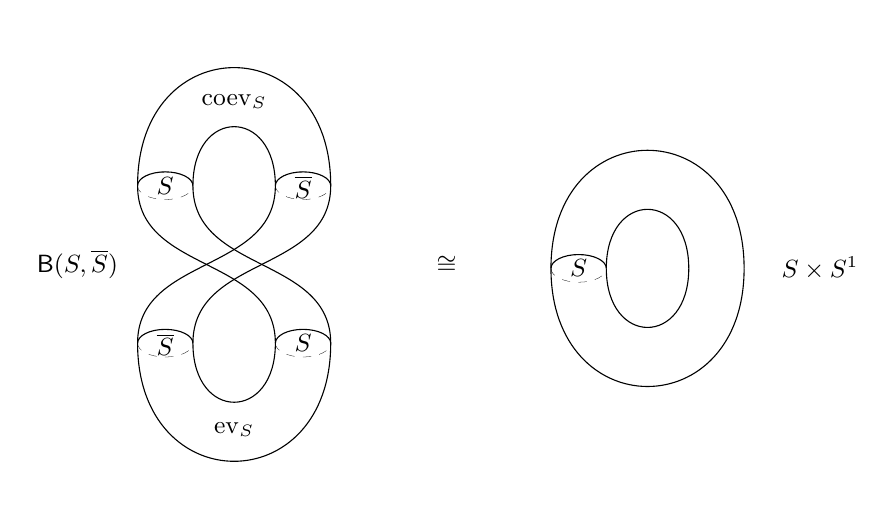
\begin{tikzpicture}[tqft/cobordism edge/.style={draw}]
  %left
  %coevaluation
  \pic[tqft,name=co,cobordism height=3cm,boundary separation=1.75cm,incoming boundary components=0,outgoing boundary components=2,every outgoing upper boundary component/.style={draw},every outgoing boundary component/.style={draw,ultra thin,dashed}];
  \node[at=(co-outgoing boundary 1),font=\small]{$S$};
  \node[at=(co-outgoing boundary 2),below=-7pt,font=\small]{$\overline{S}$};
  \node[at=(co-between outgoing 1 and 2),above=3pt,font=\small]{$\mathrm{coev}_{S}$};
  %braiding
  \pic[tqft/cylinder to next,name=l,boundary separation=3.5cm,at=(co-outgoing boundary 1)];
  \pic[tqft/cylinder to prior,name=r,boundary separation=3.5cm,at=(co-outgoing boundary 2)];
  \node[at=(r-between first incoming and first outgoing),left=1cm,font=\small]{$\mathsf{B}(S,\overline{S})$};
  %evaluation
  \pic[tqft,name=ev,cobordism height=3cm,boundary separation=1.75cm,incoming boundary components=2,outgoing boundary components=0,anchor=incoming boundary 1,at=(r-outgoing boundary 1),every incoming upper boundary component/.style={draw},every incoming lower boundary component/.style={draw,ultra thin,dashed}];
  \node[at=(ev-incoming boundary 1),below=-7pt,font=\small]{$\overline{S}$};
  \node[at=(ev-incoming boundary 2),font=\small]{$S$};
  \node[at=(ev-between incoming 1 and 2),below=4pt,font=\small]{$\mathrm{ev}_{S}$};

  %right
  \node[at=(r-between first incoming and first outgoing),right=2.8cm,font=\small]{$\cong$};
  %top
  \pic[tqft,name=co2,cobordism height=3cm,boundary separation=1.75cm,incoming boundary components=0,outgoing boundary components=2,anchor={(-1,0.65)},at=(co-outgoing boundary 2),outgoing upper boundary component 1/.style={draw},outgoing lower boundary component 1/.style={draw,ultra thin,dashed}];
  \node[at=(co2-outgoing boundary 1),font=\small]{$S$};
  %bottom
  \pic[tqft,name=ev2,cobordism height=3cm,boundary separation=1.75cm,incoming boundary components=2,outgoing boundary components=0,anchor=incoming boundary 1,at=(co2-outgoing boundary 1)];
  \node[at=(co2-outgoing boundary 2),right=2em,font=\small]{$S \times S^{1}$};
\end{tikzpicture}
\caption{Illustration of the product manifold with the circle}
\label{fig:dimcirc}
\end{figure}
\\
Using the coherence condition for $\mathsf{B}$ and $\mathsf{H}$ we find by applying $Z$ that
\begin{align*}
  &
  \Phi^{-1}
  \circ
  Z([S \times S^{1}])
  \circ
  \Phi
  \\
  &=
  \Phi^{-1}
  \circ
  Z(\mathrm{ev}_{S})
  \circ
  Z(\mathsf{B}(S,\overline{S}))
  \circ
  Z(\mathrm{coev}_{S})
  \circ
  \Phi
  \\
  &=
  \Phi^{-1}
  \circ
  Z(\mathrm{ev}_{S})
  \circ
  \mathsf{H}(\overline{S},S)
  \circ
  \mathsf{B}(Z(S),Z(\overline{S}))
  \circ
  \mathsf{H}^{-1}(S,\overline{S})
  \circ
  Z(\mathrm{coev}_{S})
  \circ
  \Phi
  \\
  &=
  \Braket{\cdot,\cdot}
  \circ
  \mathsf{B}(Z(S),Z(\overline{S}))
  \circ
  \gamma
\end{align*}
Hence, choosing bases for $Z(S)$ and $Z(\overline{S})$ as above, we have
\begin{align*}
  \Phi^{-1}
  \left(
    Z([S \times S^{1}])
    \left(
      \Phi(1)
    \right)
  \right)
  &=
  \Braket{\cdot,\cdot}
  \left(
    \mathsf{B}(Z(S),Z(\overline{S}))
    \left(
      \gamma(1)
    \right)
  \right)
  \\
  &=
  \Braket{\cdot,\cdot}
  \left(
    \mathsf{B}(Z(S),Z(\overline{S}))
    \left(
      \sum_{i = 1}^{k}
      b_{i}
      \otimes
      \bar{b}_{i}
    \right)
  \right)
  \\
  &=
  \sum_{i = 1}^{k}
  \Braket{\bar{b}_{i},b_{i}}
  \\
  &=
  k
  \\
  &=
  \dim(Z(S))
\end{align*}
finishing the proof.
\\
\phantom{proven}
\hfill
$\square$
\end{prf}


\subsection{Dimensional Reduction}
\label{subsec:dimred}
\nocite{0a816f4c}
%%%
Next, we consider a process called dimensional reduction which allows to produce many TQFTs of lower dimension from a given TQFT. This illustrates why TQFTs in higher dimensions are generally way more complicated as there are way more data involved. The higher the dimension of the given TQFT is, the more lower-dimensional TQFTs can be produced. Dimensional reduction is basically accomplished by taking the cartesian product with a fixed manifold of lower dimension and the main part is described by the following
\\
\begin{lem}
\label{lem:cobprod}
Let $X \in \mathrm{ob}_{\mathbf{DiffCOr}_{\infty}^{r}}$ be a smooth oriented closed manifold of dimension $r < n$. Consider the functions\footnote{we abuse notation here because these functions constitute a functor}
\begin{align*}
  &
  (\cdot) \times X
  \colon
  \mathrm{ob}_{\mathbf{Cob}_{n - r}}
  \to
  \mathrm{ob}_{\mathbf{Cob}_{n}}
  \\
  &
  ((\cdot) \times X)(S)
  :=
  S \times X
  \\
  &
  (\cdot) \times X
  \colon
  \mathrm{Mor}_{\mathbf{Cob}_{n - r}}
  \to
  \mathrm{Mor}_{\mathbf{Cob}_{n}}
  \\
  &
  ((\cdot) \times X)([(M,\iota_{1},\iota_{2})])
  :=
  \left[
    \left(
      M \times X
      ,
      \iota_{1}
      \times
      \mathrm{id}_{X}
      ,
      \iota_{2}
      \times
      \mathrm{id}_{X}
    \right)
  \right]
\end{align*}
and
\begin{align*}
  &
  \mathsf{H}_{X}
  \colon
  \mathrm{ob}_{\mathbf{Cob}_{n - r} \times \mathbf{Cob}_{n - r}}
  \to
  \mathrm{Mor}_{\mathbf{Cob}_{n}}
  \\
  &
  \mathsf{H}_{X}(S_{1},S_{2})
  :=
  C_{n}(h_{S_{1},S_{2}}^{X})
\end{align*}
where the latter is defined using the cylinder construction for the canonical diffeomorphism
\begin{align*}
  h_{S_{1},S_{2}}^{X}
  \colon
  (S_{1} \times X)
  \sqcup
  (S_{2} \times X)
  &
  \to
  (S_{1} \sqcup S_{2})
  \times
  X
\end{align*}
Then
\begin{align*}
  \left(
    (\cdot)
    \times
    X
    ,
    \mathsf{H}_{X}
    ,
    \mathrm{id}_{\emptyset}
  \right)
  \colon
  \mathbf{Cob}_{n - r}
  &\to
  \mathbf{Cob}_{n}
\end{align*}
is a symmetric monoidal functor where $\mathrm{id}_{\emptyset}$ is the identity for the empty $(n - 1)$-manifold in $\mathbf{Cob}_{n}$.
\end{lem}
\begin{prf}[Sketch]
We will just give a sketch here and leave the details to the diligent reader.
\begin{enumerate}
\item[i)]
The well-definedness of the functions $(\cdot) \times X$ is easy to see since the Cartesian product behaves nicely with manifolds so we take this for granted here.

\item[ii)]
The function $(\cdot) \times X$ clearly takes morphisms from $S_{1}$ to $S_{2}$ to morphisms from $S_{1} \times X$ to $S_{2} \times X$ which is necessary for $(\cdot) \times X$ to be a functor.
\\
The preservation of the identity is rather obvious since
\begin{align*}
  \left(
    S
    \times
    [0,1]
  \right)
  \times
  X
  \qquad
  \text{and}
  \qquad
  \left(
    S
    \times
    X
  \right)
  \times
  [0,1]
\end{align*}
are clearly diffeomorphic rel boundary and thus represent the same morphism.
\\
For the preservation of composition consider cobordisms
\begin{align*}
  M_{1}
  \colon
  S_{1}
  &\to
  S
  \qquad
  \text{and}
  \qquad
  M_{2}
  \colon
  S
  \to
  S_{2}
\end{align*}
glued along $S$ to yield the cobordism $M \colon S_{1} \to S_{2}$. Then it is not difficult to see that
\begin{align*}
M \times X \colon S_{1} \times X \to S_{2} \times X
\end{align*}
is equivalent to the cobordism obtained by gluing
\begin{align*}
  M_{1} \times X \colon S_{1} \times X \to S \times X
  \qquad
  \text{and}
  \qquad
  M_{2}
  \times
  X
  \colon
  S
  \times
  X
  \to
  S_{2}
  \times
  X
\end{align*}
along $S \times X$. This shows that $(\cdot) \times X$ is indeed a functor.

\item[iii)]
We have $\emptyset \times X = \emptyset$, where $\emptyset$ is regarded as the empty manifold of dimension $n - r - 1$ and $n - 1$, respectively, so that the identity $\mathrm{id}_{\emptyset}$ is indeed an isomorphism for the preservation of unit objects as demanded for monoidal functors.
\\
Further consider two cobordisms
\begin{align*}
  M_{1}
  \colon
  S_{1}
  &\to
  \tilde{S}_{1}
  \qquad
  \text{and}
  \qquad
  M_{2}
  \colon
  S_{2}
  \to
  \tilde{S}_{2}
\end{align*}
We have a canonical diffeomorphism
\begin{align*}
  (M_{1} \times X)
  \sqcup
  (M_{2} \times X)
  &\to
  (M_{1} \sqcup M_{2})
  \times
  X
\end{align*}
which yields the naturality of $\mathsf{H}_{X}$ with a similar argument as for the associator $\mathsf{A}$ in $\mathbf{Cob}_{n}$ (cf. section \ref{sec:cob} in chapter \ref{chap:defordtqft}).
\\
Moreover, we can define a functor
\begin{align*}
  \mathbf{DiffCOr}_{\infty}^{n - r - 1}
  \to
  \mathbf{DiffCOr}_{\infty}^{n - 1}
\end{align*}
doing the same as $(\cdot) \times X$ on objects and taking a morphism
\begin{align*}
  \phi
  \in
  \mathrm{mor}_{\mathbf{DiffCOr}_{\infty}^{n - r - 1}}(S_{1},S_{2})
\end{align*}
to
\begin{align*}
  \phi
  \times
  \mathrm{id}_{X}
  \in
  \mathrm{mor}_{\mathbf{DiffCOr}_{\infty}^{n - 1}}
  \left(
    S_{1}
    \times
    X
    ,
    S_{2}
    \times
    X
  \right)
\end{align*}
It is fairly evident that this is a functor and abusing notation we will again denote it by $(\cdot) \times X$. This functor and the corresponding one for cobordisms are compatible with the cylinder construction in the sense that
\begin{align*}
  C_{n}
  \circ
  ((\cdot) \times X)
  &=
  ((\cdot) \times X)
  \circ
  C_{n - r}
\end{align*}
This is obvious for objects and since
\begin{align*}
  C_{n}(\phi \times \mathrm{id}_{X})
  \qquad
  \text{and}
  \qquad
  C_{n - r}(\phi)
  \times
  X
\end{align*}
can be respectively represented by the cobordisms
\begin{align*}
  \left(
    S_{2}
    \times
    X
  \right)
  \times
  [0,1]
  \qquad
  \text{and}
  \qquad
  \left(
    S_{2}
    \times
    [0,1]
  \right)
  \times
  X
\end{align*}
for which there is an obvious equivalence, it is clear for morphisms as well. Hence the coherence conditions can be shown by using the cylinder construction: the diagram in (MF1) for the associator for example follows from the evident commuting diagram\footnote{in a slight abuse of notation we denote both associators in $\mathbf{DiffCOr}_{\infty}^{n - r - 1}$ and in $\mathbf{DiffCOr}_{\infty}^{n - 1}$ by $\mathsf{a}$ as it is clear from the context in which category they are}
\begin{equation*}
\hspace{2em}
\begin{tikzcd}[row sep=3em, column sep=9em]
  ((S_{1} \times X) \sqcup (S_{2} \times X))
  \sqcup
  (S_{3} \times X)
  \arrow{r}{\mathsf{a}(S_{1} \times X,S_{2} \times X,S_{3} \times X)}
  \arrow[swap]{d}{h_{S_{1},S_{2}}^{X} \sqcup \mathrm{id}_{S_{3} \times X}}
  &
  (S_{1} \times X)
  \sqcup
  ((S_{2} \times X) \sqcup (S_{3} \times X))
  \arrow{d}{\mathrm{id}_{S_{1} \times X} \sqcup h_{S_{2},S_{3}}^{X}}
  \\
  ((S_{1} \sqcup S_{2}) \times X)
  \sqcup
  (S_{3} \times X)
  \arrow[swap]{d}{h_{S_{1} \sqcup S_{2},S_{3}}^{X}}
  &
  (S_{1} \times X)
  \sqcup
  ((S_{2} \sqcup S_{3}) \times X)
  \arrow{d}{h_{S_{1},S_{2} \sqcup S_{3}}^{X}}
  \\
  \left(
    (S_{1} \sqcup S_{2})
    \sqcup
    S_{3}
  \right)
  \times
  X
  \arrow{r}{\mathsf{a}(S_{1},S_{2},S_{3}) \times \mathrm{id}_{X}}
  &
  \left(
    S_{1}
    \sqcup
    (S_{2} \sqcup S_{3})
  \right)
  \times
  X
\end{tikzcd}
\end{equation*}
by applying $C_{n}$ and using
\begin{align*}
  C_{n}
  \left(
    \mathsf{a}
    \left(
      S_{1}
      ,
      S_{2}
      ,
      S_{3}
    \right)
    \times
    \mathrm{id}_{X}
  \right)
  &=
  C_{n - r}(\mathsf{a}
  \left(
    S_{1}
    ,
    S_{2}
    ,
    S_{3})
  \right)
  \times
  X
\end{align*}
and that $C_{n}$ (strictly) preserves the disjoint union. A similar argument works for the other diagrams. Thus $(\cdot) \times X$ is monoidal.

\item[iv)]
The braidings for the manifolds involved are given by the cylinder constructions $C_{n - r}$ and $C_{n}$ for the canonical diffeomorphisms of the braidings\footnote{again slighty abusing notation we denote both braidings by $\mathsf{b}$ as it should always be clear from the context in which category they are} in $\mathbf{DiffCOr}_{\infty}^{n - r - 1}$ and $\mathbf{DiffCOr}_{\infty}^{n - 1}$,
\begin{align*}
  &
  \mathsf{b}(S_{1},S_{2})
  \colon
  S_{1}
  \sqcup
  S_{2}
  \to
  S_{2}
  \sqcup
  S_{1}
  \\
  &
  \text{and}
  \\
  &
  \mathsf{b}(S_{1} \times X,S_{2} \times X)
  \colon
  (S_{1} \times X)
  \sqcup
  (S_{2} \times X)
  \to
  (S_{2} \times X)
  \sqcup
  (S_{1} \times X)
\end{align*}
respectively. Composed with $(h_{S_{1},S_{2}}^{X})^{-1}$ and $h_{S_{2},S_{1}}^{X}$ the latter is the same as
\begin{align*}
  \mathsf{b}(S_{1},S_{2})
  \times
  \mathrm{id}_{X}
  \colon
  (S_{1} \sqcup S_{2})
  \times
  X
  &\to
  (S_{2} \sqcup S_{1})
  \times X
\end{align*}
that is,
\begin{align*}
  h_{S_{2},S_{1}}^{X}
  \circ
  \mathsf{b}(S_{1} \times X,S_{2} \times X)
  \circ
  (h_{S_{1},S_{2}}^{X})^{-1}
  &=
  \mathsf{b}(S_{1},S_{2})
  \times
  \mathrm{id}_{X}
\end{align*}
and applying $C_{n}$ shows that the coherence condition for the braiding is satisfied because
\begin{align*}
  C_{n}(\mathsf{b}(S_{1},S_{2}) \times \mathrm{id}_{X})
  &=
  C_{n - r}(\mathsf{b}(S_{1},S_{2}))
  \times
  X
\end{align*}
Hence $(\cdot) \times X$ is a symmetric monoidal functor, since the categories are symmetric.
\end{enumerate}
\phantom{proven}
\hfill
$\square$
\end{prf}
Now dimensional reduction is an easy corollary.
\\
\begin{cor}
\label{cor:dimred}
Let
\begin{align*}
  (Z,\mathsf{H},\Phi)
  \colon
  \mathbf{Cob}_{n}
  &\to
  \mathbf{Vec}_{K}
\end{align*}
be an $n$-dimensional TQFT and let $X \in \mathrm{ob}_{\mathbf{DiffCOr}_{\infty}^{r}}$ be a smooth oriented closed manifold of dimension $r < n$. The composition\footnote{remember that this is just the definition of composition for (symmetric) monoidal functors}
\begin{align*}
  (Z,\mathsf{H},\Phi)
  \circ
  \left(
    (\cdot)
    \times
    X
    ,
    \mathsf{H}_{X}
    ,
    \mathrm{id}_{\emptyset}
  \right)
  &=
  \left(
    Z
    \circ
    ((\cdot) \times X)
    ,
    Z(\mathsf{H}_{X}(\cdot,\cdot))
    \circ
    \mathsf{H}(\cdot \times X,\cdot \times X)
    ,
    \Phi
  \right)
\end{align*}
is an $(n - r)$-dimensional TQFT.
\end{cor}
\begin{prf}
By lemma \ref{lem:cobprod} the tuple $((\cdot) \times X,\mathsf{H}_{X},\mathrm{id}_{\emptyset})$ is a symmetric monoidal functor and since the composition of symmetric monoidal functors is again a symmetric monoidal functor there is nothing more to do here.
\\
\phantom{proven}
\hfill
$\square$
\end{prf}


\subsection{Connected Sum}
\label{subsec:consum}
\nocite{0a816f4c}
%%%
The last property we examine is about the connected sum, which is a way to produce a new connected $n$-manifold from two given connected $n$-manifolds. This means we can take two connected cobordisms and make a new one out of them. The property we consider then says that the linear map associated to the new cobordism by a TQFT can easily be calculated from the old ones, provided that a certain condition holds, namely that the state space on the $(n - 1)$-sphere $S^{n-1}$ is $1$-dimensional.
\\
We first sketch how to define this connected sum. For more details see e.g. \cite{wiki-map00000} in the article \href{http://www.map.mpim-bonn.mpg.de/Connected_sum}{Connected sum} and the references therein. Let $S_{1},S_{2}$ be objects in $\mathbf{Cob}_{n}$ and
\begin{align*}
  M_{1}
  \colon
  \emptyset
  &\to
  S_{1}
  ,\qquad
  M_{2}
  \colon
  S_{2}
  \to
  \emptyset
\end{align*}
be connected compact oriented cobordisms. To define the connected sum
\begin{align*}
  [M_{1}]
  \#
  [M_{2}]
\end{align*}
of the corresponding morphisms we cut out $n$-balls
\begin{align*}
  \mathbb{B}^{n}
  &:=
  \lbrace
    x
    \in
    \mathbb{R}^{n}
    \colon
    \Vert
    x
    \Vert
    \leq
    1
  \rbrace
\end{align*}
- or more precisely, we cut out embeddings of the $n$-ball, where the embedding into $M_{1}$ preserves orientation and the one into $M_{2}$ reverses orientation - from $M_{1}$ and $M_{2}$ to obtain cobordims
\begin{align*}
  \tilde{M_{1}}
  \colon
  S^{n-1}
  &\to
  S_{1}
  \qquad
  \text{and}
  \qquad
  \tilde{M_{2}}
  \colon
  S_{2}
  \to
  S^{n-1}
\end{align*}
Then we glue the resulting manifolds together along the resulting boundary spheres to obtain the new cobordism
\begin{align*}
  M_{1}
  \#
  M_{2}
  \colon 
  S_{2}
  &\to
  S_{1}
\end{align*}
Regarding the $n$-ball as cobordisms
\begin{align*}
  \mathbb{B}_{\dashv}^{n}
  \colon
  \emptyset
  &\to
  S^{n-1}
  \qquad
  \text{and}
  \qquad
  \mathbb{B}_{\vdash}^{n}
  \colon
  S^{n-1}
  \to
  \emptyset
\end{align*}
respectively (see figure \ref{fig:nballs} for an illustration), this means that we have
\begin{align*}
  [M_{1}]
  &=
  [\tilde{M_{1}}]
  \circ
  [\mathbb{B}_{\dashv}^{n}]
  ,\qquad
  [M_{2}]
  =
  [\mathbb{B}_{\vdash}^{n}]
  \circ
  [\tilde{M_{2}}]
\end{align*}
and the \textbf{connected sum} is defined by
\begin{align*}
  [M_{1}] \# [M_{2}]
  &:=
  [M_{1} \# M_{2}]
  :=
  [\tilde{M_{1}}]
  \circ
  [\tilde{M_{2}}]
\end{align*}
Using the disc theorem one can show that this construction is unique up to diffeomorphism, that is, does not depend on the chosen embeddings of the $n$-ball, so that the resulting morphism in $\mathbf{Cob}_{n}$ is well-defined. Moreover, the resulting morphism is connected which means that one and thus each cobordism representing the morphism is connected. The idea now is that when the state space of $S^{n-1}$ is $1$-dimensional then a TQFT yields, up to a constant, the same result for the composition of $M_{1}$ and $M_{2}$ and their connected sum. See figure \ref{fig:consumexa} for an illustration. This is because the state space for the empty $(n-1)$-manifold is $1$-dimensional, too, and linear maps between $1$-dimensional vector spaces cannot do more than multiplying by a constant when fixing bases.
\\
\begin{figure}[h!]
\centering
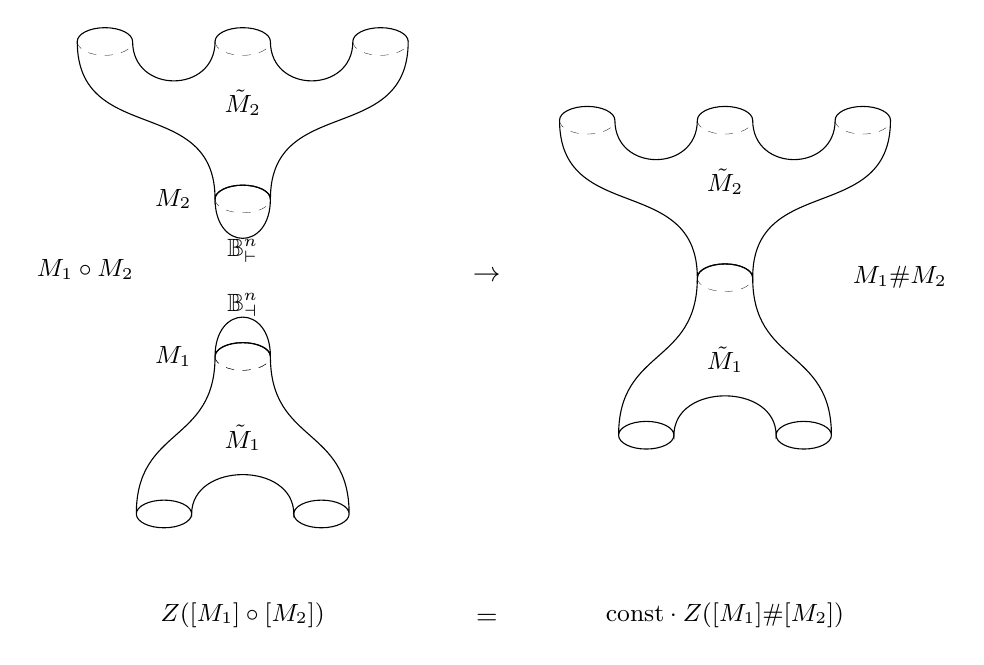
\begin{tikzpicture}[tqft/cobordism/.style={draw}]
  %left
  %top
  \pic[tqft,name=rtp,boundary separation=1.75cm,incoming boundary components=3,outgoing boundary components=1,offset=1,every incoming lower boundary component/.style={draw,ultra thin,dashed}];
  \node[at=(rtp-incoming boundary 2),below=14pt,font=\small]{$\tilde{M}_{2}$};
  \node[at=(rtp-outgoing boundary 1),left=15pt,font=\small]{$M_{2}$};
  \pic[tqft/cup,name=cup,at=(rtp-outgoing boundary 1),every incoming lower boundary component/.style={draw,ultra thin,dashed}];
  \node[at=(cup-incoming boundary 1),below=11pt,font=\small]{$\mathbb{B}_{\vdash}^{n}$};
  \node[at=(rtp-outgoing boundary 1),left=2cm,below=0.65cm,font=\small]{$M_{1} \circ M_{2}$};
  %bottom
  \pic[tqft/cap,name=cap,anchor={(1,0)},at=(rtp-outgoing boundary 1),every outgoing lower boundary component/.style={draw,ultra thin,dashed}];
  \node[at=(cap-outgoing boundary 1),above=11pt,font=\small]{$\mathbb{B}_{\dashv}^{n}$};
  \node[at=(cap-outgoing boundary 1),left=15pt,font=\small]{$M_{1}$};
  \pic[tqft/pair of pants,name=p,at=(cap-outgoing boundary 1),every incoming lower boundary component/.style={draw,ultra thin,dashed},every outgoing lower boundary component/.style={draw}];
  \node[at=(p-between outgoing 1 and 2),above=5pt,font=\small]{$\tilde{M}_{1}$};
  
  %right
  \node[at=(rtp-outgoing boundary 1),right=3.1cm,below=0.8cm]{$\to$};
  %top
  \pic[tqft,name=rtp2,anchor={(-2.5,-0.5)},at=(rtp-incoming boundary 1),boundary separation=1.75cm,incoming boundary components=3,outgoing boundary components=1,offset=1,every incoming lower boundary component/.style={draw,ultra thin,dashed}];
  \node[at=(rtp2-incoming boundary 2),below=14pt,font=\small]{$\tilde{M}_{2}$};
  \node[at=(rtp2-outgoing boundary 1),right=1.5cm,font=\small]{$M_{1} \# M_{2}$};
  %bottom
  \pic[tqft/pair of pants,name=p2,at=(rtp2-outgoing boundary 1),every incoming lower boundary component/.style={draw,ultra thin,dashed},every outgoing lower boundary component/.style={draw}];
  \node[at=(p2-between outgoing 1 and 2),above=5pt,font=\small]{$\tilde{M}_{1}$};

  %equation
  \node[at=(p-between outgoing 1 and 2),below=1.5cm,font=\small]{$Z([M_{1}] \circ [M_{2}])$};
  \node[at=(rtp-outgoing boundary 1),right=3.1cm,below=5.15cm]{$=$};
  \node[at=(p2-between outgoing 1 and 2),below=2.5cm,font=\small]{$\mathrm{const} \cdot Z([M_{1}] \# [M_{2}])$};
\end{tikzpicture}
\caption{Illustration of the calculation of a TQFT for the connected sum}
\label{fig:consumexa}
\end{figure}
\\
More precisely, we have the following
\\
\begin{thm}
\label{thm:consum}
Let
\begin{align*}
  Z
  \colon
  \mathbf{Cob}_{n}
  &\to
  \mathbf{Vec}_{K}
\end{align*}
be a TQFT with
\begin{align*}
  \dim(Z(S^{n-1}))
  &=
  1
\end{align*}
Then
\begin{align*}
\Phi^{-1}(Z([S^{n}])(\Phi(1))) \neq 0
\end{align*}
and for $S_{1},S_{2} \in \mathrm{ob}_{\mathbf{Cob}_{n}}$ and connected
\begin{align*}
  [M_{1}]
  \in
  \mathrm{mor}_{\mathbf{Cob}_{n}}(\emptyset,S_{1})
  ,\qquad
  [M_{2}]
  \in
  \mathrm{mor}_{\mathbf{Cob}_{n}}(S_{2},\emptyset)
\end{align*}
we have
\begin{align*}
  Z([M_{1}] \# [M_{2}])
  &=
  \frac{1}{\Phi^{-1}(Z([S^{n}])(\Phi(1)))}
  Z([M_{1}])
  \circ
  Z([M_{2}])
\end{align*}
\end{thm}
\begin{prf}
We keep using the notation from the definition of the connected sum above. First note that
\begin{align*}
  [\mathbb{B}_{\vdash}^{n}]
  \circ
  [\mathbb{B}_{\dashv}^{n}]
  \colon
  \emptyset
  &\to
  \emptyset
\end{align*}
can be represented by the $n$-sphere $S^{n} \colon \emptyset \to \emptyset$, as illustrated in figure \ref{fig:nballs}, which means
\begin{align*}
  Z([\mathbb{B}_{\vdash}^{n}])
  \circ
  Z([\mathbb{B}_{\dashv}^{n}])
  &=
  Z([\mathbb{B}_{\vdash}^{n}] \circ [\mathbb{B}_{\dashv}^{n}])
  \\
  &=
  Z([S^{n}])
\end{align*}
\begin{figure}[h!]
\centering
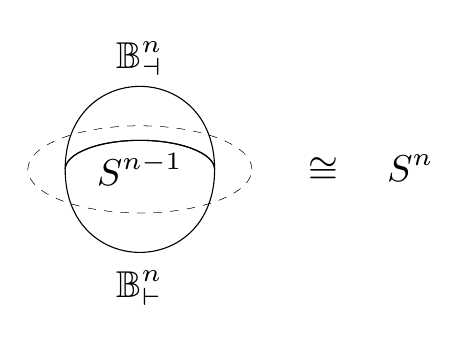
\begin{tikzpicture}[every node/.style={scale=1.5},tqft/cobordism/.style={draw}]
  %left
  %top
  \pic[tqft/cap,name=bu,cobordism height=8em,circle x radius=1.8em,circle y radius=0.7em,every outgoing boundary component/.style={draw,ultra thin,dashed}];
  \node[at=(bu-outgoing boundary 1),font=\small]{$S^{n-1}$};
  \node[at=(bu-outgoing boundary 1),above=1.9em,font=\small]{$\mathbb{B}_{\dashv}^{n}$};
  %bottom
  \pic[tqft/cup,name=bd,at=(bu-outgoing boundary 1),cobordism height=8em,circle x radius=1.8em,circle y radius=0.7em,every incoming boundary component/.style={draw,ultra thin,dashed}];
  \node[at=(bd-incoming boundary 1),below=2.1em,font=\small]{$\mathbb{B}_{\vdash}^{n}$};

  %right
  \node[at=(bu-outgoing boundary 1),right=1.3cm,font=\small]{$\cong \quad S^{n}$};
\end{tikzpicture}
\caption{Gluing two $n$-balls together yields an $n$-sphere}
\label{fig:nballs}
\end{figure}
\\
Since $Z(S^{n-1})$ is $1$-dimensional we can choose a basis element, say $e$, and then we have
\begin{align*}
  Z([\mathbb{B}_{\dashv}^{n}])(\Phi(1))
  &=
  b_{\dashv}
  e
  ,\qquad
  \Phi^{-1}
  \left(
    Z([\mathbb{B}_{\vdash}^{n}])(e)
  \right)
  =
  b_{\vdash}
  ,\qquad
  Z([\tilde{M_{2}}])(v)
  =
  c(v)
  e
\end{align*}
for certain $b_{\dashv},b_{\vdash},c(v) \in K$ and all $v \in Z(S_{2})$. With this and the linearity of all involved maps we can easily calculate
\begin{align*}
  &
  \left(
    Z([\tilde{M_{1}}])
    \circ
    Z([\mathbb{B}_{\dashv}^{n}])
    \circ
    Z([\mathbb{B}_{\vdash}^{n}])
    \circ
    Z([\tilde{M_{2}}])
  \right)
  (v)
  \\
  &=
  c(v)
  \left(
    Z([\tilde{M_{1}}])
    \circ
    Z([\mathbb{B}_{\dashv}^{n}])
    \circ
    Z([\mathbb{B}_{\vdash}^{n}])
  \right)
  (e)
  \\
  &=
  b_{\vdash}
  c(v)
  \left(
    Z([\tilde{M_{1}}])
    \circ
    Z([\mathbb{B}_{\dashv}^{n}])
  \right)
  (\Phi(1))
  \\
  &=
  b_{\dashv}
  b_{\vdash}
  c(v)
  Z([\tilde{M_{1}}])(e)
  \\
  &=
  b_{\dashv}
  \Phi^{-1}
  \left(
    Z([\mathbb{B}_{\vdash}^{n}])(e)
  \right)
  Z([\tilde{M_{1}}])(c(v)e)
  \\
  &=
  \Phi^{-1}
  \left(
    Z([\mathbb{B}_{\vdash}^{n}])(b_{\dashv}e)
  \right)
  \left(
    Z([\tilde{M_{1}}])
    \circ
    Z([\tilde{M_{2}}])
  \right)
  (v)
  \\
  &=
  \Phi^{-1}
  \left(
    \left(
      Z([\mathbb{B}_{\vdash}^{n}])
      \circ
      Z([\mathbb{B}_{\dashv}^{n}])
    \right)
    (\Phi(1))
  \right)
  \left(
    Z([\tilde{M_{1}}])
    \circ
    Z([\tilde{M_{2}}])
  \right)
  (v)
\end{align*}
This shows that
\begin{align*}
  Z([M_{1}])
  \circ
  Z([M_{2}])
  &=
  Z([\tilde{M_{1}}])
  \circ
  Z([\mathbb{B}_{\dashv}^{n}])
  \circ
  Z([\mathbb{B}_{\vdash}^{n}])
  \circ
  Z([\tilde{M_{2}}])
  \\
  &=
  \Phi^{-1}
  \left(
    \left(
      Z([\mathbb{B}_{\vdash}^{n}])
      \circ
      Z([\mathbb{B}_{\dashv}^{n}])
    \right)
    (\Phi(1))
  \right)
  \left(
    Z([\tilde{M_{1}}])
    \circ
    Z([\tilde{M_{2}}])
  \right)
  \\
  &=
  \Phi^{-1}
  \left(
    Z([S^{n}])(\Phi(1))
  \right)
  Z([M_{1}] \# [M_{2}])
\end{align*}
If we can show that
\begin{align*}
  \Phi^{-1}(Z([S^{n}])(\Phi(1)))
  &\neq
  0
\end{align*}
then we are done. To this end suppose
\begin{align*}
  \Phi^{-1}(Z([S^{n}])(\Phi(1)))
  &=
  0
\end{align*}
then the above equation implies
\begin{align*}
  Z([M_{1}]) \circ Z([M_{2}])
  &=
  0
\end{align*}
for all $S_{1},S_{2} \in \mathrm{ob}_{\mathbf{Cob}_{n}}$ and connected
\begin{align*}
  [M_{1}]
  \in
  \mathrm{mor}_{\mathbf{Cob}_{n}}(\emptyset,S_{1})
  ,\qquad
  [M_{2}]
  \in
  \mathrm{mor}_{\mathbf{Cob}_{n}}(S_{2},\emptyset)
\end{align*}
To bring this to a contradiction let
\begin{align*}
  [M_{1}]
  &:=
  \mathrm{coev}_{\overline{S^{n-1}}}
  \qquad
  \text{and}
  \qquad
  [M_{2}]
  :=
  \mathrm{ev}_{S^{n-1}}
\end{align*}
which are both clearly connected. Consider the morphisms $X$ and $Y$ defined by making the following diagrams commute
\begin{equation*}
\hspace{-4em}
\begin{tikzcd}[row sep=5em,column sep=6em]
  S^{n-1}
  \sqcup
  (\overline{S^{n-1}} \sqcup S^{n-1})
  \ar{r}{X}
  \ar{d}[swap]{\mathsf{A}^{-1}(S^{n-1},\overline{S^{n-1}},S^{n-1})}
  &
  S^{n-1}
  \\
  (S^{n-1} \sqcup \overline{S^{n-1}})
  \sqcup
  S^{n-1}
  \ar{r}{\mathrm{ev}_{\overline{S^{n-1}}} \sqcup \mathrm{id}_{S^{n-1}}}
  &
  \emptyset
  \sqcup
  S^{n-1}
  \ar{u}[swap]{\mathsf{L}(S^{n-1})}
\end{tikzcd}
\end{equation*}
\begin{equation*}
\hspace{4em}
\begin{tikzcd}[row sep=5em,column sep=6em]
  S^{n-1}
  \ar{r}{Y}
  \ar{d}[swap]{\mathsf{L}^{-1}(S^{n-1})}
  &
  S^{n-1}
  \sqcup
  (\overline{S^{n-1}} \sqcup S^{n-1})
  \\
  \emptyset
  \sqcup
  S^{n-1}
  \ar{r}{\mathrm{coev}_{S^{n-1}} \sqcup \mathrm{id}_{S^{n-1}}}
  &
  (S^{n-1} \sqcup \overline{S^{n-1}})
  \sqcup
  S^{n-1}
  \ar{u}[swap]{\mathsf{A}(S^{n-1},\overline{S^{n-1}},S^{n-1})}
\end{tikzcd}
\end{equation*}
where we used $\overline{\overline{S^{n-1}}} = S^{n-1}$ in the first diagram. We will show that
\begin{align}
\label{diffcyl}
  X
  \circ
  \left(
    \mathrm{id}_{S^{n-1}}
    \sqcup
    \left(
      \mathrm{coev}_{\overline{S^{n-1}}}
      \circ
      \mathrm{ev}_{S^{n-1}}
    \right)
  \right)
  \circ
  Y
  &=
  \mathrm{id}_{S^{n-1}}
\end{align}
See figure \ref{fig:s1contr} for an illustration with the associativity and unit cylinders suppressed.
\\
\begin{figure}[h!]
\centering
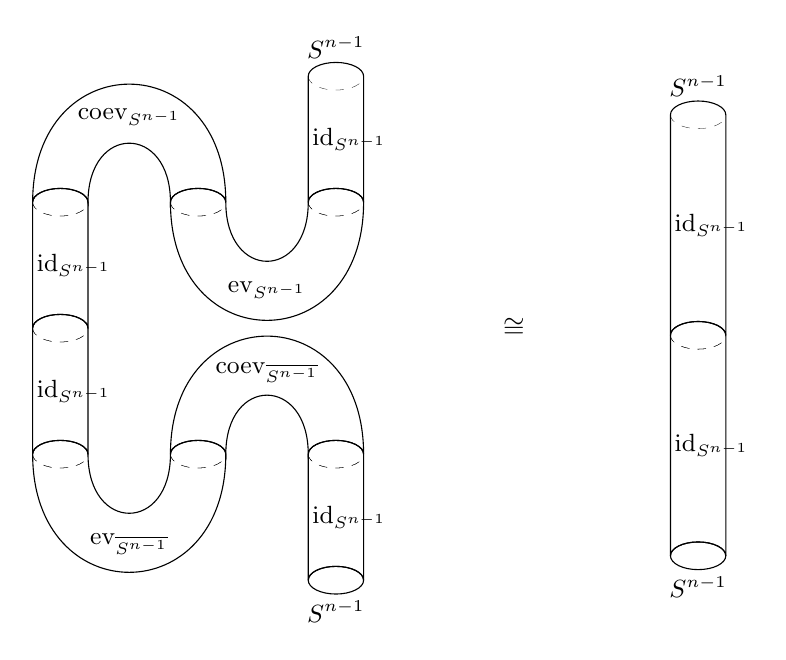
\begin{tikzpicture}[tqft/cobordism/.style={draw}]
  %left
  %coevaluation
  \pic[tqft,name=co,cobordism height=3cm,boundary separation=1.75cm,incoming boundary components=0,outgoing boundary components=2,every outgoing boundary component/.style={draw,ultra thin,dashed}];
  \node[at=(co-between outgoing 1 and 2),above=3pt,font=\small]{$\mathrm{coev}_{S^{n-1}}$};
  %evaluation
  \pic[tqft,name=ev,cobordism height=3cm,boundary separation=1.75cm,incoming boundary components=2,outgoing boundary components=0,anchor=incoming boundary 1,at=(co-outgoing boundary 2),every incoming lower boundary component/.style={draw,ultra thin,dashed}];
  \node[at=(ev-between incoming 1 and 2),below=4pt,font=\small]{$\mathrm{ev}_{S^{n-1}}$};
  %cylinders
  \pic[tqft/cylinder,name=c1,cobordism height=1.6cm,anchor=outgoing boundary 1,at=(ev-incoming boundary 2),every incoming lower boundary component/.style={draw,ultra thin,dashed},every outgoing boundary component/.style={draw,ultra thin,dashed}];
  \node[at=(c1-incoming boundary 1),above=3pt,font=\small]{$S^{n-1}$};
  \node[at=(c1-between first incoming and first outgoing),right=-2pt,font=\small]{$\mathrm{id}_{S^{n-1}}$};
  \pic[tqft/cylinder,name=c2,cobordism height=1.6cm,anchor=incoming boundary 1,at=(co-outgoing boundary 1),every incoming lower boundary component/.style={draw,ultra thin,dashed},every outgoing boundary component/.style={draw,ultra thin,dashed}];
  \node[at=(c2-between first incoming and first outgoing),right=-2pt,font=\small]{$\mathrm{id}_{S^{n-1}}$};
  \pic[tqft/cylinder,name=c3,cobordism height=1.6cm,anchor=incoming boundary 1,at=(c2-outgoing boundary 1),every incoming lower boundary component/.style={draw,ultra thin,dashed},every outgoing boundary component/.style={draw,ultra thin,dashed}];
  \node[at=(c3-between first incoming and first outgoing),right=-2pt,font=\small]{$\mathrm{id}_{S^{n-1}}$};
  %opposite evaluation
  \pic[tqft,name=evop,cobordism height=3cm,boundary separation=1.75cm,incoming boundary components=2,outgoing boundary components=0,anchor=incoming boundary 1,at=(c3-outgoing boundary 1),every incoming lower boundary component/.style={draw,ultra thin,dashed}];
  \node[at=(evop-between incoming 1 and 2),below=4pt,font=\small]{$\mathrm{ev}_{\overline{S^{n-1}}}$};
  %opposite coevaluation
  \pic[tqft,name=coop,cobordism height=3cm,boundary separation=1.75cm,incoming boundary components=0,outgoing boundary components=2,anchor=outgoing boundary 1,at=(evop-incoming boundary 2),every outgoing boundary component/.style={draw,ultra thin,dashed}];
  \node[at=(coop-between outgoing 1 and 2),above=1pt,font=\small]{$\mathrm{coev}_{\overline{S^{n-1}}}$};
  %cylinder
  \pic[tqft/cylinder,name=c4,cobordism height=1.6cm,anchor=incoming boundary 1,at=(coop-outgoing boundary 2),every incoming lower boundary component/.style={draw,ultra thin,dashed},every outgoing boundary component/.style={draw}];
  \node[at=(c4-outgoing boundary 1),below=4pt,font=\small]{$S^{n-1}$};
  \node[at=(c4-between first incoming and first outgoing),right=-2pt,font=\small]{$\mathrm{id}_{S^{n-1}}$};

  %right
  \node[at=(c2-outgoing boundary 1),right=5.5cm]{$\cong$};
  %top
  \pic[tqft/cylinder,name=c5,cobordism height=2.8cm,anchor={(-1.3,-0.175)},at=(c1-incoming boundary 1),every incoming lower boundary component/.style={draw,ultra thin,dashed},every outgoing boundary component/.style={draw,ultra thin,dashed}];
  \node[at=(c5-incoming boundary 1),above=3pt,font=\small]{$S^{n-1}$};
  \node[at=(c5-between first incoming and first outgoing),right=-2pt,font=\small]{$\mathrm{id}_{S^{n-1}}$};
  %bottom
  \pic[tqft/cylinder,name=c6,cobordism height=2.8cm,anchor=incoming boundary 1,at=(c5-outgoing boundary 1),every incoming lower boundary component/.style={draw,ultra thin,dashed},every outgoing boundary component/.style={draw}];
  \node[at=(c6-outgoing boundary 1),below=4pt,font=\small]{$S^{n-1}$};
  \node[at=(c6-between first incoming and first outgoing),right=-2pt,font=\small]{$\mathrm{id}_{S^{n-1}}$};
\end{tikzpicture}
\caption{Illustration of equation \eqref{diffcyl}}
\label{fig:s1contr}
\end{figure}
\newpage
By definition we have the outer perimeter of the following commuting diagram. The lower part follows from the functoriality of $\sqcup$, the lower left part follows from diagram (LD1) for $\mathrm{coev}_{S^{n-1}}$ and $\mathrm{ev}_{S^{n-1}}$ and the lower right part follows from diagram (LD2) for $\mathrm{coev}_{\overline{S^{n-1}}}$ and $\mathrm{ev}_{\overline{S^{n-1}}}$. The central part obviously commutes and hence so does the upper part proving equation \eqref{diffcyl}.
\begin{equation*}
\begin{tikzcd}[row sep=5em,column sep=6em,font=\footnotesize,every label/.append style={font=\tiny}]
  S^{n-1}
  \sqcup
  (\overline{S^{n-1}} \sqcup S^{n-1})
  \ar{rr}{\mathrm{id}_{S^{n-1}} \sqcup (\mathrm{coev}_{\overline{S^{n-1}}} \circ \mathrm{ev}_{S^{n-1}})}
  &
  &
  S^{n-1}
  \sqcup
  (\overline{S^{n-1}} \sqcup S^{n-1})
  \ar{d}{X}
  \\
  S^{n-1}
  \ar{u}{Y}
  \ar{rr}{\mathrm{id}_{S^{n-1}}}
  \ar{rddd}{\mathsf{R}^{-1}(S^{n-1})}
  \ar{d}[swap]{\mathsf{L}^{-1}(S^{n-1})}
  &
  &
  S^{n-1}
  \\
  \emptyset
  \sqcup
  S^{n-1}
  \ar{d}[swap]{\mathrm{coev}_{S^{n-1}} \sqcup \mathrm{id}_{S^{n-1}}}
  &
  &
  \emptyset
  \sqcup
  S^{n-1}
  \ar{u}[swap]{\mathsf{L}(S^{n-1})}
  \\
  (S^{n-1} \sqcup \overline{S^{n-1}})
  \sqcup
  S^{n-1}
  \ar{d}[swap]{\mathsf{A}(S^{n-1},\overline{S^{n-1}},S^{n-1})}
  &
  &
  (S^{n-1} \sqcup \overline{S^{n-1}})
  \sqcup
  S^{n-1}
  \ar{u}[swap]{\mathrm{ev}_{\overline{S^{n-1}}} \sqcup \mathrm{id}_{S^{n-1}}}
  \\
  S^{n-1}
  \sqcup
  (\overline{S^{n-1}} \sqcup S^{n-1})
  \ar{r}{\mathrm{id}_{S^{n-1}} \sqcup \mathrm{ev}_{S^{n-1}}}
  \ar[bend right]{rr}[yshift=4pt]{\mathrm{id}_{S^{n-1}} \sqcup (\mathrm{coev}_{\overline{S^{n-1}}} \circ \mathrm{ev}_{S^{n-1}})}
  &
  S^{n-1}
  \sqcup
  \emptyset
  \ar{uuur}{\mathsf{R}(S^{n-1})}
  \ar{r}{\mathrm{id}_{S^{n-1}} \sqcup \mathrm{coev}_{\overline{S^{n-1}}}}
  &
  S^{n-1}
  \sqcup
  (\overline{S^{n-1}} \sqcup S^{n-1})
  \ar{u}[swap]{\mathsf{A}^{-1}(S^{n-1},\overline{S^{n-1}},S^{n-1})}
\end{tikzcd}
\end{equation*}
Now we apply $Z$ to equation \eqref{diffcyl} which yields zero for the left-hand side since
\begin{align*}
  &
  Z
  \left(
    \mathrm{id}_{S^{n-1}}
    \sqcup
    \left(
      \mathrm{coev}_{\overline{S^{n-1}}}
      \circ
      \mathrm{ev}_{S^{n-1}}
    \right)
  \right)
  \\
  &=
  \mathsf{H}
  \left(
    S^{n-1}
    ,
    \overline{S^{n-1}} \sqcup S^{n-1}
  \right)
  \circ
  \left(
    Z(\mathrm{id}_{S^{n-1}})
    \otimes
    \left(
      Z(\mathrm{coev}_{\overline{S^{n-1}}})
      \circ
      Z(\mathrm{ev}_{S^{n-1}})
    \right)
  \right)
  \circ
  \mathsf{H}^{-1}
  \left(
    S^{n-1}
    ,
    \overline{S^{n-1}} \sqcup S^{n-1}
  \right)
  \\
  &=
  \mathsf{H}
  \left(
    S^{n-1}
    ,
    \overline{S^{n-1}} \sqcup S^{n-1}
  \right)
  \circ
  \left(
    \mathrm{id}_{Z(S^{n-1})}
    \otimes
    0
  \right)
  \circ
  \mathsf{H}^{-1}
  \left(
    S^{n-1}
    ,
    \overline{S^{n-1}} \sqcup S^{n-1}
  \right)
  \\
  &=
  0
\end{align*}
but for the right-hand side we obtain $\mathrm{id}_{Z(S^{n-1})}$ which is not zero since $\dim(Z(S^{n-1})) = 1$. This contradiction shows that
\begin{align*}
  \Phi^{-1}(Z(S^{n})(\Phi(1)))
  &\neq
  0
\end{align*}
and finishes our proof.
\\
\phantom{proven}
\hfill
$\square$
\end{prf}
Thus if the state space of the sphere $S^{n-1}$ for a TQFT is $1$-dimensional we have another way to calculate the linear map associated to a cobordism provided it can be written as the connected sum of two connected cobordisms where one has empty in-boundary and one has empty out-boundary.





\part{Close Encounters of the Higher Kind}
\label{part:higher}
%\nocite{cc6d78b5}
%\nocite{dfcdc48c}
%%%
So far we have seen the categorical definition of ordinary TQFTs and some of their basic properties. Now one may wonder how many such TQFTs exist and whether they can be classified in some, more or less, efficient way. For 1-dimensional TQFTs it is easy to give such a description very explicitly and for 2-dimensional TQFTs it is not too difficult either to find a classification in terms of algebraic objects. With increasing dimension however things become more and more complicated and one is lead to extended TQFTs which involve a more sophisticated version of the cobordism category.
\\
As already mentioned in the motivation in chapter \ref{chap:motqft} these extended TQFTs are what one really aims for from a physical point of view because they allow to cut spacetime not only in the time direction but also in the spatial directions. Thus they do not break general covariance as ordinary TQFTs do.
\\
The cobordism hypothesis - formulated in its original incarnation by Baez and Dolan in \cite{cc6d78b5} - now basically states that the more sophisticated cobordism category used for extended TQFTs has a rather simple algebraic description and thereby gives sort of a classification for extended TQFTs.
\\
These notions are naturally cast in the language of higher categories which first needs to be made precise. As this is rather involved we will treat higher categories on an informal level here which nevertheless should capture the idea.
\\
Lurie gives a formulation for the cobordism hypothesis and a rather detailed sketch of the proof in \cite{dfcdc48c}. Even though a fully detailed account is missing the proof is widely accepted by the experienced community.
\\\\
This part of the present work is based on this expository paper \cite{dfcdc48c} by Lurie and the objective here is to sufficiently prepare the reader to understand the formulation of the cobordism hypothesis as given there and how one arrives at this formulation. We do not, however, discuss the proof.
\\\\
There are again four chapters in this part. The first one is chapter \ref{chap:prelim2} where we start with some preliminaries we need in the following chapters. In chapter \ref{chap:lowdimtqft} we discuss low-dimensional ordinary TQFTs in order to see how one is led to extended TQFTs. The subsequent chapter \ref{chap:extcob} is about extending the ordinary category of cobordims to obtain the higher category of cobordisms mentioned above. Finally, in chapter \ref{chap:formcobhyp} we formulate different versions of the cobordism hypothesis.





\chapter{Preliminaries}
\label{chap:prelim2}
\stepcounter{prpcounter}
This preliminary chapter consists of two sections. In section \ref{sec:highcat} we introduce higher categories. As giving a precise definition of higher categories is rather involved we content ourselves with an informal treatment trying to make clear what a higher category is supposed to be and to provide some intuition. Moreover, we introduce some constructions and properties on this informal level which we need later in the text. Along the way we give some references containing more details for the notions introduced here. Section \ref{sec:mancorn} then is about manifolds with corners which are a generalization of the concept of manifolds with boundary. After introducing the basic concept we discuss how one can define higher cobordisms which are basically cobordisms between cobordisms.



\section{Higher Categories}
\label{sec:highcat}
%\nocite{6f59ab3c}
%\nocite{9094cf60}
%\nocite{d37d0fca}
%\nocite{dfcdc48c}
%\nocite{f3c68a99}
%\nocite{0349e8ea}
%\nocite{00000001}
%%%
As the natural language for the formulation of the cobordism hypothesis is that of higher categories we want to give a description of them here. However, we do it in an informal way, trying to give the reader a good idea of the concept rather than a precise definition as the latter needs some concepts we have not introduced here.
\\\\
An ordinary category $\mathbf{C}$ basically consists of a set of objects $\mathrm{ob}_{\mathbf{C}}$ and for any two objects $X_{1},X_{2} \in \mathrm{ob}_{\mathbf{C}}$ a set of morphisms $\mathrm{mor}_{\mathbf{C}}(X_{1},X_{2})$ between them. Moreover, there is a composition $\circ_{\mathbf{C}}$ for morphisms, usually simply written $\circ$, producing a morphism
\begin{align*}
  f_{13}
  &=
  f_{23}
  \circ
  f_{12}
  \in
  \mathrm{mor}_{\mathbf{C}}(X_{1},X_{3})
\end{align*}
from two morphisms $f_{12} \in \mathrm{mor}_{\mathbf{C}}(X_{1},X_{2})$ and $f_{23} \in \mathrm{mor}_{\mathbf{C}}(X_{2},X_{3})$ for any $X_{1},X_{2},X_{3} \in \mathrm{ob}_{\mathbf{C}}$. This composition is associative and unital, where the latter means that for every object $X_{1} \in \mathrm{ob}_{\mathbf{C}}$ there is an identity morphism $\mathrm{id}_{X_{1}}$ for the composition.
\\
However, there may also be relations between the morphisms, as is the case, for example, when considering the category $\mathbf{Cat}$ of small categories and functors between them. Then we have natural transformations as relations between morphisms but we cannot include them into $\mathbf{Cat}$ unless we allow an additional layer of morphisms in the concept of categories. This leads to the notion of a (strict) $2$-category ${_{2}\mathbf{C}}$, which basically can be described as follows
\begin{enumerate}
\item[(0)]
we have a set of objects $\mathrm{ob}_{{_{2}\mathbf{C}}}$, sometimes also referred to as $0$-morphisms and written ${_{0}}\mathrm{mor}_{{_{2}\mathbf{C}}}$

\item[(1)]
for any two objects $X_{1},X_{2} \in {_{0}}\mathrm{mor}_{{_{2}\mathbf{C}}}$ we have a set ${_{1}}\mathrm{mor}_{{_{2}\mathbf{C}}}(X_{1},X_{2})$ of $1$-morphisms between them

\item[(2)]
for any two parallel $1$-morphisms $f_{12},f_{12}^{\backprime} \in {_{1}}\mathrm{mor}_{{_{2}\mathbf{C}}}(X_{1},X_{2})$ - which means $1$-morphisms between the same objects - we have a set ${_{2}}\mathrm{mor}_{{_{2}\mathbf{C}}}(X_{1},X_{2},f_{12},f_{12}^{\backprime})$ of $2$-morphisms between them. We ususally depict such a $2$-morphism by a double arrow as in the following diagram
\begin{equation*}
\begin{tikzcd}[row sep=2.4em,column sep=5.6em]
  X_{1}
  \ar[bend left=50]{r}[swap,name=U]{}{f_{12}}
  \ar[bend right=50]{r}[name=D]{}[swap]{f_{12}^{\backprime}}
  &
  X_{2}
  \ar[Rightarrow,from=U,to=D]
\end{tikzcd}
\end{equation*}

\item[(c)]
there are different associative and unital compositions on the level of $1$-morphisms and $2$-morphisms
\begin{enumerate}
\item[(1)]
composition for $1$-morphisms, written $\circ$, is just as in the case of an ordinary category

\item[(2)]
$2$-morphisms can be composed in two directions, vertically and horizontally
\begin{enumerate}
\item[(v)]
the vertical composition $\circ^{\mathrm{v}}$ is along $1$-morphisms, i.e. for $2$-morphisms
\begin{align*}
\hspace{7em}
  \alpha_{1}
  \in
  {_{2}}\mathrm{mor}_{{_{2}\mathbf{C}}}
  \left(
    X_{1}
    ,
    X_{2}
    ,
    f_{12}
    ,
    f_{12}^{\backprime}
  \right)
  \qquad
  \text{and}
  \qquad
  \alpha_{2} \in {_{2}}\mathrm{mor}_{{_{2}\mathbf{C}}}
  \left(
    X_{1}
    ,
    X_{2}
    ,
    f_{12}^{\backprime}
    ,
    f_{12}^{\backprime\backprime}
  \right)
\end{align*}
we obtain a $2$-morphism
\begin{align*}
\hspace{2em}
  \alpha_{2}
  \circ^{\mathrm{v}}
  \alpha_{1}
  &\in
  {_{2}}\mathrm{mor}_{{_{2}\mathbf{C}}}
  \left(
    X_{1}
    ,
    X_{2}
    ,
    f_{12}
    ,
    f_{12}^{\backprime\backprime}
  \right)
\end{align*}
as in the following diagram
\begin{equation*}
\hspace{7em}
\begin{tikzcd}[row sep=2.4em,column sep=12em]
  X_{1}
  \ar[bend left=50]{r}[swap,name=U1]{}{f_{12}}
  \ar{r}[name=D1]{}[swap]{f_{12}^{\backprime}}[swap,below=5.5mm,font=\normalsize]{\circ^{\mathrm{v}}}
  &
  X_{2}
  \ar[Rightarrow,from=U1,to=D1,"\alpha_{1}"]
  \\
  X_{1}
  \ar{r}[swap,name=U2]{}{f_{12}^{\backprime}}
  \ar[bend right=50]{r}[name=D2]{}[swap]{f_{12}^{\backprime\backprime}}
  &
  X_{2}
  \ar[Rightarrow,from=U2,to=D2,"\alpha_{2}"]
\end{tikzcd}
  \quad
  =
  \quad
\begin{tikzcd}[row sep=2.4em,column sep=12em]
  X_{1}
  \ar[bend left=60]{r}[swap,name=U]{}{f_{12}}
  \ar{r}[name=M1]{f_{12}^{\backprime}}[swap,name=M2]{f_{12}^{\backprime}}
  \ar[bend right=60]{r}[name=D]{}[swap]{f_{12}^{\backprime\backprime}}
  &
  X_{2}
  \ar[Rightarrow,from=U,to=M1,"\alpha_{1}"]
  \ar[Rightarrow,from=M2,to=D,"\alpha_{2}"]
\end{tikzcd}
\end{equation*}
Unitality of the vertical composition means that for every $1$-morphism $f_{12} \in {_{1}}\mathrm{mor}_{{_{2}\mathbf{C}}}(X_{1},X_{2})$ there is a $2$-morphism 
\begin{align*}
\hspace{7em}
  \mathrm{id}_{f_{12}}
  \in
  {_{2}}\mathrm{mor}_{{_{2}\mathbf{C}}}
  \left(
    X_{1}
    ,
    X_{2}
    ,
    f_{12}
    ,
    f_{12}
  \right)
\end{align*}
which is an identity of the vertical composition, i.e. for $\alpha_{1} \in {_{2}}\mathrm{mor}_{{_{2}\mathbf{C}}}(X_{1},X_{2},f_{12},f_{12}^{\backprime})$ we have
\begin{equation*}
\hspace{7em}
\begin{tikzcd}[row sep=2.4em,column sep=12em]
  X_{1}
  \ar[bend left=60]{r}[swap,name=U]{}{f_{12}}
  \ar{r}[name=M1]{f_{12}^{\backprime}}[swap,name=M2]{f_{12}^{\backprime}}
  \ar[bend right=60]{r}[name=D]{}[swap]{f_{12}^{\backprime}}
  &
  X_{2}
  \ar[Rightarrow,from=U,to=M1,"\alpha_{1}"]
  \ar[Rightarrow,from=M2,to=D,"\mathrm{id}_{f_{12}^{\backprime}}"]
\end{tikzcd}
  \quad
  =
  \quad
\begin{tikzcd}[row sep=2.4em,column sep=5.6em]
  X_{1}
  \ar[bend left=50]{r}[swap,name=U]{}{f_{12}}
  \ar[bend right=50]{r}[name=D]{}[swap]{f_{12}^{\backprime}}
  &
  X_{2}
  \ar[Rightarrow,from=U,to=D,"\alpha_{1}"]
\end{tikzcd}
\end{equation*}
and
\begin{equation*}
\hspace{7em}
\begin{tikzcd}[row sep=2.4em,column sep=12em]
  X_{1}
  \ar[bend left=60]{r}[swap,name=U]{}{f_{12}}
  \ar{r}[name=M1]{f_{12}}[swap,name=M2]{f_{12}}
  \ar[bend right=60]{r}[name=D]{}[swap]{f_{12}^{\backprime}}
  &
  X_{2}
  \ar[Rightarrow,from=U,to=M1,"\mathrm{id}_{f_{12}}"]
  \ar[Rightarrow,from=M2,to=D,"\alpha_{1}"]
\end{tikzcd}
  \quad
  =
  \quad
\begin{tikzcd}[row sep=2.4em,column sep=5.6em]
  X_{1}
  \ar[bend left=50]{r}[swap,name=U]{}{f_{12}}
  \ar[bend right=50]{r}[name=D]{}[swap]{f_{12}^{\backprime}}
  &
  X_{2}
  \ar[Rightarrow,from=U,to=D,"\alpha_{1}"]
\end{tikzcd}
\end{equation*}

\item[(h)]
the horizontal composition $\circ^{\mathrm{h}}$ is along $0$-morphisms, i.e. for $2$-morphisms
\begin{align*}
\hspace{7em}
  \alpha_{12}
  \in
  {_{2}}\mathrm{mor}_{{_{2}\mathbf{C}}}
  \left(
    X_{1}
    ,
    X_{2}
    ,
    f_{12}
    ,
    f_{12}^{\backprime}
  \right)
  \qquad
  \text{and}
  \qquad
  \alpha_{23}
  \in
  {_{2}}\mathrm{mor}_{{_{2}\mathbf{C}}}
  \left(
    X_{2}
    ,
    X_{3}
    ,
    f_{23}
    ,
    f_{23}^{\backprime}
  \right)
\end{align*}
we obtain a $2$-morphism
\begin{align*}
\hspace{7em}
  \alpha_{23}
  \circ^{\mathrm{h}}
  \alpha_{12}
  &\in
  {_{2}}\mathrm{mor}_{{_{2}\mathbf{C}}}
  \left(
    X_{1}
    ,
    X_{3}
    ,
    f_{23} \circ f_{12}
    ,
    f_{23}^{\backprime}
    \circ
    f_{12}^{\backprime}
  \right)
\end{align*}
as in the following diagram
\begin{equation*}
\hspace{3em}
\begin{tikzcd}[row sep=2.4em,column sep=5.6em]
  X_{1}
  \ar[bend left=50]{r}[swap,name=U1]{}{f_{12}}
  \ar[bend right=50]{r}[name=D1]{}[swap]{f_{12}^{\backprime}}
  &
  X_{2}
  \ar[Rightarrow,from=U1,to=D1,"\alpha_{12}"]
\end{tikzcd}
  \circ^{\mathrm{h}}
\begin{tikzcd}[row sep=2.4em,column sep=5.6em]
  X_{2}
  \ar[bend left=50]{r}[swap,name=U2]{}{f_{23}}
  \ar[bend right=50]{r}[name=D2]{}[swap]{f_{23}^{\backprime}}
  &
  X_{3}
  \ar[Rightarrow,from=U2,to=D2,"\alpha_{23}"]
\end{tikzcd}
  \quad
  =
  \quad
\begin{tikzcd}[row sep=2.4em,column sep=5.6em]
  X_{1}
  \ar[bend left=50]{r}[swap,name=U1]{}{f_{12}}
  \ar[bend right=50]{r}[name=D1]{}[swap]{f_{12}^{\backprime}}
  &
  X_{2}
  \ar[Rightarrow,from=U1,to=D1,"\alpha_{12}"]
  \ar[bend left=50]{r}[swap,name=U2]{}{f_{23}}
  \ar[bend right=50]{r}[name=D2]{}[swap]{f_{23}^{\backprime}}
  &
  X_{3}
  \ar[Rightarrow,from=U2,to=D2,"\alpha_{23}"]
\end{tikzcd}
\end{equation*}
The identities for the horizontal composition are given by the identity $2$-morphisms of the identity $1$-morphisms of the corresponding objects, that is, for a $2$-morphism $\alpha_{1} \in {_{2}}\mathrm{mor}_{{_{2}\mathbf{C}}}(X_{1},X_{2},f_{12},f_{12}^{\backprime})$ we have
\begin{equation*}
\hspace{3em}
\begin{tikzcd}[row sep=2.4em,column sep=5.6em]
  X_{1}
  \ar[bend left=50]{r}[swap,name=U1]{}{f_{12}}
  \ar[bend right=50]{r}[name=D1]{}[swap]{f_{12}^{\backprime}}
  &
  X_{2}
  \ar[Rightarrow,from=U1,to=D1,"\alpha_{12}"]
  \ar[bend left=50]{r}[swap,name=U2]{}{\mathrm{id}_{X_{2}}}
  \ar[bend right=50]{r}[name=D2]{}[swap]{\mathrm{id}_{X_{2}}}
  &
  X_{2}
  \ar[Rightarrow,from=U2,to=D2,"\mathrm{id}_{\mathrm{id}_{X_{2}}}"]
\end{tikzcd}
  \quad
  =
  \quad
\begin{tikzcd}[row sep=2.4em,column sep=5.6em]
  X_{1}
  \ar[bend left=50]{r}[swap,name=U]{}{f_{12}}
  \ar[bend right=50]{r}[name=D]{}[swap]{f_{12}^{\backprime}}
  &
  X_{2}
  \ar[Rightarrow,from=U,to=D,"\alpha_{12}"]
\end{tikzcd}
\end{equation*}
and
\begin{equation*}
\hspace{3em}
\begin{tikzcd}[row sep=2.4em,column sep=5.6em]
  X_{1}
  \ar[bend left=50]{r}[swap,name=U2]{}{\mathrm{id}_{X_{1}}}
  \ar[bend right=50]{r}[name=D2]{}[swap]{\mathrm{id}_{X_{1}}}
  &
  X_{1}
  \ar[Rightarrow,from=U2,to=D2,"\mathrm{id}_{\mathrm{id}_{X_{1}}}"]
  \ar[bend left=50]{r}[swap,name=U1]{}{f_{12}}
  \ar[bend right=50]{r}[name=D1]{}[swap]{f_{12}^{\backprime}}
  &
  X_{2}
  \ar[Rightarrow,from=U1,to=D1,"\alpha_{12}"]
\end{tikzcd}
  \quad
  =
  \quad
\begin{tikzcd}[row sep=2.4em,column sep=5.6em]
  X_{1}
  \ar[bend left=50]{r}[swap,name=U]{}{f_{12}}
  \ar[bend right=50]{r}[name=D]{}[swap]{f_{12}^{\backprime}}
  &
  X_{2}
  \ar[Rightarrow,from=U,to=D,"\alpha_{12}"]
\end{tikzcd}
\end{equation*}
\end{enumerate}
The two ways of composing $2$-morphisms are independent in the sense that they commute, i.e. when composing in both directions it does not matter in which direction we start, which means that the diagrams
\begin{equation*}
\hspace{5em}
\begin{tikzcd}[row sep=2.4em,column sep=12em]
  X_{1}
  \ar[bend left=60]{r}[swap,name=U]{}{f_{12}}
  \ar{r}[name=M1]{f_{12}^{\backprime}}[swap,name=M2]{f_{12}^{\backprime}}
  \ar[bend right=60]{r}[name=D]{}[swap]{f_{12}^{\backprime\backprime}}
  &
  X_{2}
  \ar[Rightarrow,from=U,to=M1,"\alpha_{1}"]
  \ar[Rightarrow,from=M2,to=D,"\alpha_{3}"]
\end{tikzcd}
  \quad
  \circ^{\mathrm{h}}
  \quad
\begin{tikzcd}[row sep=2.4em,column sep=12em]
  X_{2}
  \ar[bend left=60]{r}[swap,name=U]{}{f_{23}}
  \ar{r}[name=M1]{f_{23}^{\backprime}}[swap,name=M2]{f_{23}^{\backprime}}
  \ar[bend right=60]{r}[name=D]{}[swap]{f_{23}^{\backprime\backprime}}
  &
  X_{3}
  \ar[Rightarrow,from=U,to=M1,"\alpha_{2}"]
  \ar[Rightarrow,from=M2,to=D,"\alpha_{4}"]
\end{tikzcd}
\end{equation*}
and
\begin{equation*}
\begin{tikzcd}[row sep=2.4em,column sep=12em]
  X_{1}
  \ar[bend left=60]{r}[swap,name=U1]{}{f_{12}}
  \ar{r}[name=M1]{}[swap]{f_{12}^{\backprime}}[swap,below=7mm,right=25mm,font=\normalsize]{\circ^{\mathrm{v}}}
  &
  X_{2}
  \ar[bend left=60]{r}[swap,name=U2]{}{f_{23}}
  \ar{r}[name=M2]{}[swap]{f_{23}^{\backprime}}
  &
  X_{3}
  \ar[Rightarrow,from=U1,to=M1,"\alpha_{1}"]
  \ar[Rightarrow,from=U2,to=M2,"\alpha_{2}"]
  \\
  X_{1}
  \ar{r}[swap,name=U3]{}{f_{12}^{\backprime}}
  \ar[bend right=60]{r}[name=M3]{}[swap]{f_{12}^{\backprime\backprime}}
  &
  X_{2}
  \ar{r}[swap,name=M4]{}{f_{23}^{\backprime}}
  \ar[bend right=60]{r}[name=D4]{}[swap]{f_{23}^{\backprime\backprime}}
  &
  X_{3}
  \ar[Rightarrow,from=U3,to=M3,"\alpha_{3}"]
  \ar[Rightarrow,from=M4,to=D4,"\alpha_{4}"]
\end{tikzcd}
\end{equation*}
depict the same $2$-morphism. This latter property is often referred to as the exchange law or interchange law.
\end{enumerate}
\end{enumerate}
In the case of $\mathbf{Cat}$ we add the natural transformations between functors as $2$-morphisms and hence obtain the (strict) $2$-category ${_{2}}\mathbf{Cat}$.
\\
If we require composition at both levels to be associative, unital and interchanging on the nose, as in the case of ${_{2}}\mathbf{Cat}$, we obtain the notion of strict $2$-categories which are rather easy to define precisely. Closer investigation of the structure above shows that we have a set of objects and for any two objects a category of morphisms between them. The objects of that category are interpreted as $1$-morphisms, the morphisms are interpreted as $2$-morphisms and the composition is the vertical composition of $2$-morphisms. In addition, for every three objects there is a functor between the corresponding morphism categories which encodes the composition of $1$-morphisms and the horizontal composition of $2$-morphisms (see e.g. \cite{00000001} for a spelled out description). The functoriality of the horizontal composition ensures that the interchange law is satisfied. More concisely a strict $2$-category can be defined to be a category enriched in small categories (see e.g. \cite{00000001}).
\\\\
Now why should we stop at level $2$? We can generalize the notion of $2$-categories to the notion of \textit{$n$-categories} for any $n \in \mathbb{N}$ by adding layers up to level $n$, i.e. we basically have
\begin{enumerate}
\item[(0)]
a set of objects

\item[(1)]
for any pair of objects $X_{1},X_{2}$ a set of $1$-morphisms from $X_{1}$ to $X_{2}$

\item[(2)]
for any pair of objects $X_{1},X_{2}$ and any pair of parallel $1$-morphisms $f_{1},f_{2}$ from $X_{1}$ to $X_{2}$ a set of $2$-morphisms from $f_{1}$ to $f_{2}$

\item[]
\begin{equation*}
\vdots
\end{equation*}
\item[]

\item[(n)]
for any pair of objects $X_{1},X_{2}$ and any pair of parallel $1$-morphisms $f_{1},f_{2}$ from $X_{1}$ to $X_{2}$ ... and any pair of parallel $(n-1)$-morphisms $\alpha_{1},\alpha_{2}$ a set of $n$-morphisms from $\alpha_{1}$ to $\alpha_{2}$

\item[(c)]
at each level $0 \leq k \leq n$ an associative and unital composition in $k$ interchanging directions, one direction along which $k$-morphisms can be composed for each level below $k$
\end{enumerate}
In particular a $0$-category is just a set and a $1$-category is just an ordinary category. Again, in the case that composition at each level is associative, unital and interchanging on the nose we obtain the notion of strict $n$-categories which are fairly easy to define precisely. Namely we can inductively define a strict $n$-category to be a category enriched in small $(n-1)$-categories. One may also go another way and use internalization\footnote{see e.e. \cite{00000001} for the idea of internalization} to define category objects internal to $\mathbf{Cat}$ which yields so called double categories. In order to obtain a $2$-category in the above sense one has to impose a further condition but then one can iterate this process of internalization to define $n$-categories. We will not press the details on this further here.
\\
Functors between categories are generalized to $n$-categories in the way one would probably expect: an \textit{$n$-functor}, usually only called functor, from an $n$-category ${_{n}}\mathbf{C}$ to an $n$-category ${_{n}}\mathbf{C}_{\alpha}$ takes objects in ${_{n}}\mathbf{C}$ to objects in ${_{n}}\mathbf{C}_{\alpha}$, $1$-morphisms in ${_{n}}\mathbf{C}$ to $1$-morphisms in ${_{n}}\mathbf{C}_{\alpha}$, ... and $n$-morphisms in ${_{n}}\mathbf{C}$ to $n$-morphisms in ${_{n}}\mathbf{C}_{\alpha}$ in a functorial way, that is, such that compositions and identities are respected at all levels. More concisely one can say that an $n$-functor takes $k$-morphisms in ${_{n}}\mathbf{C}$ to $k$-morphisms in ${_{n}}\mathbf{C}_{\alpha}$ for $0 \leq k < n+1$ in a functorial way. Similarly, natural transformations between functors are generalized to \textit{$n$-natural transformations} between $n$-functors, taking $k$-morphisms in ${_{n}}\mathbf{C}$ to $(k+1)$-morphisms in ${_{n}}\mathbf{C}_{\alpha}$ for $0 \leq k < n$ in a natural way. But now that there are more levels of morphisms, there is a more general concept subsuming that of functors and natural transformations, namely that of \textit{$m$-transfors}\footnote{the word transfor is a portmanteau of the words functor and transformation} of $n$-categories, sometimes also called $(n,m)$-transfors. For $0 \leq m < n+1$ an $m$-transfor from ${_{n}}\mathbf{C}$ to ${_{n}}\mathbf{C}_{\alpha}$ is an operation that takes $k$-morphisms, $0 \leq k < n-m+1$, in ${_{n}}\mathbf{C}$ to $(k+m)$-morphisms in ${_{n}}\mathbf{C}_{\alpha}$ while satisfying conditions of functoriality and naturality. For $m \geq 1$ the source and target of an $m$-transfor are $(m-1)$-transfors and the naturality conditions are satisfied w.r.t. them. An $n$-functor is hence a $0$-transfor and an $n$-natural transformation is a $1$-transfor. If we depict the morphism levels of an $n$-category ${_{n}}\mathbf{C}$ as follows
\begin{equation*}
\begin{tikzcd}[sep=tiny]
  {_{0}}\mathrm{Mor}_{{_{n}}\mathbf{C}}
  \\
  \vdots
  \\
  {_{n}}\mathrm{Mor}_{{_{n}}\mathbf{C}}
\end{tikzcd}
\end{equation*}
then for $n$-categories ${_{n}}\mathbf{C}$ and ${_{n}}\mathbf{C}_{\alpha}$ we can illustrate an $m$-transfor as\footnote{here we assumed $n-m > m+m$ which of course is not necessarily the case}
\begin{equation*}
\begin{tikzcd}[row sep=tiny,column sep=large]
  {_{0}}\mathrm{Mor}_{{_{n}}\mathbf{C}}
  \arrow{rdd}{}
  &
  {_{0}}\mathrm{Mor}_{{_{n}}\mathbf{C}_{\alpha}}
  \\
  \vdots
  &
  \vdots
  \\
  {_{m}}\mathrm{Mor}_{{_{n}}\mathbf{C}}
  \arrow{rdd}{}
  &
  {_{m}}\mathrm{Mor}_{{_{n}}\mathbf{C}_{\alpha}}
  \\
  \vdots
  &
  \vdots
  \\
  \vdots
  &
  {_{m+m}}\mathrm{Mor}_{{_{n}}\mathbf{C}_{\alpha}}
  \\
  \vdots
  &
  \vdots
  \\
  {_{n-m}}\mathrm{Mor}_{{_{n}}\mathbf{C}}
  \arrow{rdd}{}
  &
  \vdots
  \\
  \vdots
  &
  \vdots
  \\
  {_{n}}\mathrm{Mor}_{{_{n}}\mathbf{C}}
  &
  {_{n}}\mathrm{Mor}_{{_{n}}\mathbf{C}_{\alpha}}
\end{tikzcd}
\end{equation*}
We will not pursue further details here.
\\
One can also imagine to allow layers of morphisms at arbitrary levels (of natural numbers) which leads to the notion of \textit{strict $\infty$-categories} which also often go by the name (strict) $\omega$-categories. The precise definition here is a bit more difficult than in the case of finitely many layers.
\\\\
Contemplating examples of higher categories one quickly realizes that the notion of strict $n$-categories is too narrow and one would rather like to have some kind of weak enrichment or internalization: for most of the interesting examples composition is, for example, not associative on the nose but rather only up to equivalence, i.e. there is an isomorphism on level $k$ between two different bracketings of the composition of three $(k-1)$-morphisms. In order to still reasonably speak of an associative composition one should require that this reassociation happens in a coherent way, which basically means that when rebracketing longer expressions it should not really matter in what order the rebrackting is done so that any two ways of rebracketing are again (coherently) isomorphic, i.e. equivalent. This leads to the notion of \textit{weak $n$-categories} in which composition is associative, unital and interchanging only up to equivalence. Again, just to be clear, {\glqq}up to equivalence{\grqq} means that there is a morphism one level above the structure in question which conveys the equivalence and this higher morphism is invertible - again weakly, i.e. only up to equivalence - and satisfies some coherence conditions, also in a weak way. Thus, this weak notion of equivalence is of a somewhat recursive nature. Equality only exists on the level of $n$-morphisms, i.e. the highest morphism level, because there are no higher morphisms that can convey a weak equivalence. For a weak $2$-category, often also called bicategory, the coherence conditions can be spelled out explicitly with reasonable effort (see e.g. \cite{00000001} or the appendix of \cite{d37d0fca}) and they are basically the same as the ones of monoidal categories. For higher weak $n$-categories it becomes more and more difficult to handle the coherence laws. There are many different proposed definitions of weak $n$-categories but it is not generally clear whether they are equivalent.
\\
However, there is a somewhat different approach for which there has been a lot of progress in recent years, namely that of \textit{$(\infty,n)$-categories} for $n \in \mathbb{N}$. Here we have a \textit{weak $\infty$-category}, i.e. morphisms at aribtrary levels and weak compositions everywhere, but all $k$-morphisms for $k > n$ are required to be weakly invertible, that is invertible up to equivalence which means up to higher weakly invertible morphisms in a coherent way all the way up. Note that now there is no highest level of morphisms anymore, so that equivalence always goes really all the way up and there is no equality at all anymore. A bit more spelled out we can describe the structure schematically as having
\begin{enumerate}
\item[(0)]
a set of objects

\item[(1)]
for any pair of objects $X_{1},X_{2}$ a set of $1$-morphisms from $X_{1}$ to $X_{2}$

\item[(2)]
for any pair of objects $X_{1},X_{2}$ and any pair of parallel $1$-morphisms $f_{1},f_{2}$ from $X_{1}$ to $X_{2}$ a set of $2$-morphisms from $f_{1}$ to $f_{2}$

\item[]
\begin{equation*}
\vdots
\end{equation*}
\item[]

\item[(n)]
for any pair of objects $X_{1},X_{2}$ and any pair of parallel $1$-morphisms $f_{1},f_{2}$ from $X_{1}$ to $X_{2}$ ... and any pair of parallel $(n-1)$-morphisms $\alpha_{1},\alpha_{2}$ a set of $n$-morphisms from $\alpha_{1}$ to $\alpha_{2}$

\item[(n+1)]
for any pair of objects $X_{1},X_{2}$ and any pair of parallel $1$-morphisms $f_{1},f_{2}$ from $X_{1}$ to $X_{2}$ ... and any pair of parallel $n$-morphisms $\nu_{1},\nu_{2}$ a set of weakly invertible $(n+1)$-morphisms from $\nu_{1}$ to $\nu_{2}$

\item[]
\begin{equation*}
\vdots
\end{equation*}
\item[]

\item[(...)]
all higher morphisms are weakly invertible

\item[]
\begin{equation*}
\vdots
\end{equation*}
\item[]

\item[(c)]
at each level $k \in \mathbb{N}$ a weakly associative and weakly unital composition in $k$ weakly interchanging directions, one direction along which $k$-morphisms can be composed for each level below $k$
\end{enumerate}
\textit{Functors between $(\infty,n)$-categories} of course act on all morphism levels and functoriality is understood in a weak sense and similar for more general \textit{transfors of $(\infty,n)$-categories}. An illustration of an $m$-transfor of $(\infty,n)$-categories ${_{(\infty,n)}}\mathbf{C}$ and ${_{(\infty,n)}}\mathbf{C}_{\alpha}$ then looks as follows
\begin{equation*}
\begin{tikzcd}[row sep=tiny,column sep=large]
  {_{0}}\mathrm{Mor}_{{_{(\infty,n)}}\mathbf{C}}
  \arrow{rdd}{}
  &
  {_{0}}\mathrm{Mor}_{{_{(\infty,n)}}\mathbf{C}_{\alpha}}
  \\
  \vdots
  &
  \vdots
  \\
  {_{m}}\mathrm{Mor}_{{_{(\infty,n)}}\mathbf{C}}
  \arrow{rdd}{}
  &
  {_{m}}\mathrm{Mor}_{{_{(\infty,n)}}\mathbf{C}_{\alpha}}
  \\
  \vdots
  &
  \vdots
  \\
  \vdots
  &
  {_{m+m}}\mathrm{Mor}_{{_{(\infty,n)}}\mathbf{C}_{\alpha}}
  \\
  \vdots
  &
  \vdots
  \\
  {_{n}}\mathrm{Mor}_{{_{(\infty,n)}}\mathbf{C}}
  \arrow{rdd}{}
  &
  \vdots
  \\
  {_{n+1}}\mathrm{Mor}_{{_{(\infty,n)}}\mathbf{C}}
  \arrow{rdd}{}
  &
  \vdots
  \\
  \vdots
  &
  {_{n+m}}\mathrm{Mor}_{{_{(\infty,n)}}\mathbf{C}_{\alpha}}
  \\
  \vdots
  &
  {_{n+m+1}}\mathrm{Mor}_{{_{(\infty,n)}}\mathbf{C}_{\alpha}}
  \\
  \vdots
  &
  \vdots
\end{tikzcd}
\end{equation*}
\\
Now one may wonder how it could be helpful to allow morphisms at arbitrary levels, as we suggested above that it is already not that easy to define strict $\infty$-categories, let alone weak ones. The point is that we do not need a general definition of weak $\infty$-categories because all morphisms above level $n$ are weakly invertible. Here homotopy-theoretical methods come to our help as we will explain in the following. From now on we adopt the convention that composition is weak unless stated otherwise.
\\
We first focus more closely on $(\infty,0)$-categories, often referred to as \textit{$\infty$-groupoids}. According to the homotopy hypothesis the notion of $\infty$-groupoids is basically equivalent to the notion of topological spaces by means of the fundamental $\infty$-groupoid construction. In principle this construction proceeds as follows
\\
\begin{cst}
\label{cst:fundinfgrpd}
Given a topological space $X$ its \textit{fundamental $\infty$-groupoid} $\pi_{\leq\infty}X$ can be described in the following way
\begin{enumerate}
\item[(0)]
the objects are the points of $X$

\item[(1)]
for two objects $x_{1},x_{2}$ a $1$-morphism from $x_{1}$ to $x_{2}$ is a path from $x_{1}$ to $x_{2}$ in $X$

\item[(2)]
for two objects $x_{1},x_{2}$ and two parallel $1$-morphisms $f_{1},f_{2} \colon x_{1} \to x_{2}$ a $2$-morphism from $f_{1}$ to $f_{2}$ is a homotopy of paths in $X$ (which we require to be fixed at the common endpoints)

\item[]
\begin{equation*}
\vdots
\end{equation*}
\item[]

\item[(k)]
higher morphisms are higher homotopies between lower ones (fixed on the common boundaries)

\item[]
\begin{equation*}
\vdots
\end{equation*}
\item[]

\item[(c)]
composition\footnote{see e.g. \cite{00000001} for a bit more on this} at all levels is given by patching homotopies together along common boundaries in the various directions
\end{enumerate}
\end{cst}
As homotopies are invertible up to higher homotopies and the compositions are associative, unital and interchanging up to higher homotopies this is indeed an $\infty$-groupoid. The homotopy hypothesis may be stated as follows
\\
\begin{prp}[Homotopy Hypothesis]
\label{prp:homhyp}
Construction \ref{cst:fundinfgrpd}, which takes a topological space $X$ to its fundamental $\infty$-groupoid $\pi_{\leq\infty}X$, establishes a bijection between topological spaces up to weak homotopy equivalence and $\infty$-groupoids up to equivalence.
\end{prp}
Therefore one possibility is to define an $\infty$-groupoid to be a topological space. There are other possible definitions. For another, more combinatorial approach note that the classical homotopy theory of topological spaces is the same as the classical homotopy theory of simplicial sets in the sense that the corresponding model categories are Quillen equivalent\footnote{model categories are a setting for doing kind of abstract homotopy theory and Quillen equivalence is the corresponding notion of equivalence of such abstract homotopy theories}. Thus it is reasonable to take simplicial sets, or more precisely \textit{Kan complexes} which are the so-called fibrant objects in the classical model structure on simplicial sets, as the definition of $\infty$-groupoids. Whatever definition is taken, the homotopy hypothesis should be understood as a consistency condition for the definition to be reasonable. In some sense it can be seen as a litmus test for whether the coherence conditions are properly encoded. 
\\
With a good model for the definition of an $\infty$-groupoid at hand we can try to use some kind of enrichment (or internalization) to define $(\infty,n)$-categories inductively, i.e. an $(\infty,n)$-category is kind of a category enriched in $(\infty,n-1)$-categories (or kind of a category object internal to $(\infty,n-1)$-categories). But as we want composition to be weak rather than strict we would once again like to have a weak process of enrichment or internalization. This may seem to get us into the same troubles as before, yet the structure of $(\infty,n)$-categories can be handled much more easily compared to the structure of weak $n$-categories even though the former are more general: the theory of $(\infty,n)$-categories subsumes the theory of \textit{$(m,n)$-categorie}s, $m \geq n$, i.e. of categories with morphisms up to level $m$ but only invertible ones above level $n$. The latter can be viewed as the special case of the former in which all $k$-morphisms with $k > m$ are trivial, i.e. identities, or to put it differently, any two parallel $k$-morphisms are equivalent for $k > m$. Weak $n$-categories are then obtained as the special case of $(n,n)$-categories. The reason why $(\infty,n)$-categories are easier to define and handle than $(m,n)$-categories for finite $m$ is that for the former it is not necessary to demand anything to be equal on the nose but only that some spaces ($\infty$-groupoids) of choices, like that for the associator with its higher coherence morphisms, is contractible. In this context one also speaks of things {\glqq}up to infinite coherent homotopy{\grqq}, like associative up to infinite coherent homotopy. For $(m,n)$-categories without morphisms above level $m$ one has to demand some of these spaces of higher morphisms to be exactly equal to a single point space which is more difficult to control than just being contractible.
\\
There are different very well-understood models, i.e. precise definitions in terms of concrete mathematical objects, of $(\infty,1)$-categories using homotopy-theoretic tools such as simplicial objects. Here the coherence laws can be nicely packaged into the definition. An $(\infty,1)$-category can to some extent be viewed as an abstract homotopy theory:
\begin{enumerate}
\item[(c)]
in classical homotopy theory one is concerned with topological spaces, continuous functions between them and classical homotopies between these continuous functions and iteratively higher homotopies

\item[(a)]
in an $(\infty,1)$-category there are objects, $1$-morphisms between them and higher weakly invertible morphisms between these $1$-morphisms and on all levels above which can be interpreted as homotopies
\end{enumerate}
In this light one sometimes speaks of categories up to coherent homotopy. However, there is actually a bit more to classical homotopy theory, namely the objects have the structure of spaces and in particular allow for homotopy groups. Thus, one might argue that the objects of an $(\infty,1)$-category considered as abstract homotopy theory should have a structure of some kind of generalized spaces, which leads to the notion of \textit{$(\infty,1)$-topoi} as a setting for abstract homotopy theory (see e.g. \cite{00000001} and the references therein for a bit more on ($(\infty,1)$-)topoi). The classical homotopy theory can be viewed as a special case of this abstract notion in a certain sense by considering the category $\mathbf{Top}$ of topological spaces homotopically as an $(\infty,1)$-category, for example by \textit{simplicial localization} at weak homotopy equivalences. This basically means that the objects and morphisms of the ordinary category $\mathbf{Top}$ are contained in the resulting $(\infty,1)$-category, denoted $\mathrm{L}\mathbf{Top}$, in such a way that all weak homotopy equivalences are equivalences in the sense of $1$-morphisms in $(\infty,1)$-categories, i.e. they are invertible up to coherent homotopy. Note that the simplicial localization is to be distinguished from viewing the ordinary category $\mathbf{Top}$ as an $(\infty,1)$-category with only trivial morphisms above level $1$ in which case the homotopical information is not built into the higher morphisms.
\\
The above-mentioned models for $(\infty,1)$-categories can be compared using model structures and are known to be equivalent from a homotopy-theoretic point of view via Quillen equivalences. These models can be generalized to yield models for $(\infty,n)$-categories in many different ways and many of them are by now well-understood and have also been shown to be equivalent. In comparison, the theory of \textit{$(\infty,\infty)$-categories}\footnote{this is a less ambiguous notation for weak $\infty$-categories mentioned before} is currently rather poorly understood. There are several proposed definitions for what an $(\infty,\infty)$-category is but it does not really seem to be clear what the right morphisms between $(\infty,\infty)$-categories are.
\\
For a good overview and many references for details of some of these models for $(\infty,n)$-categories see e.g. \cite{f3c68a99}. That survey does not cover all models but there are many references to models that are not covered. Moreover, there are references to the axiomatic approaches of To\"en, in the $(\infty,1)$-case, and Barwick and Schommer-Pries \cite{6f59ab3c}, in the more general $(\infty,n)$-case. This axiomatic approach is accomplished within a specific model of $(\infty,1)$-categories, namely the model of quasicategories since this one is currently the most-developed one by far. In fact, most of basic category theory has been extended by Joyal, Lurie and others (see e.g. \cite{0349e8ea} for an extensive account) from ordinary categories to $(\infty,1)$-categories using the specific model of quasicategories. This extension is done in such a way that the obtained quasicategorical notions reduce to the ordinary categorical notions when considered on ordinary categories. Now a quasicategory satisfying some reasonable axioms is called a theory of $(\infty,n)$-categories in \cite{6f59ab3c} and the authors of the paper show that all such theories are equivalent and that many of the models for $(\infty,n)$-categories are theories in this sense.
\\
As there are so many different models, a natural question is whether the choice of model matters for constructions and theorems about $(\infty,n)$-categories? In particular, is it possible to transfer all the results accomplished in the model of quasicategories to other models for $(\infty,1)$-categories? At least for the models that are equivalent from a homotopy-theoretic point of view the choice of model should not really matter. To make this precise in a systematic way there is a rather new, and still rapidly-evolving as the authors say, {\glqq}model-independent{\grqq} approach by Riehl and Verity \cite{53e76732}. They use a special model of $(\infty,2)$-categories - namely categories enriched in quasicategories satisfying some axioms, then called $\infty$-cosmoi - as an ambient framework in which higher category theory is developed. The objects in such an $\infty$-cosmos are then called $\infty$-categories (recast as a technical term) and their results hold for any model of higher categories fitting into the framework, i.e. for any model satisfying the axioms of $\infty$-categories in this sense. This is known to include several of the above-mentioned models for $(\infty,1)$-categories - in particular quasicategories - and moreover some models for $(\infty,n)$-categories and more models may be added. In addition to the model-independent results there are {\glqq}change-of-model{\grqq} functors called biequivalences which allow to transfer theorems proven within a specific model to any other biequivalent model. One may expect that the above-mentioned models which are known to be equivalent in the homotopy-theoretic sense by Quillen equivalences are also biequivalent and indeed, it is known that some of the above models of $(\infty,1)$-categories are biequivalent. Hence the whole theory of quasicategories can be transferred to them (and the other way around).
\\
The particular model used in \cite{dfcdc48c} for the formulation of the cobordism hypothesis is that of $n$-fold complete Segal spaces because it is rather well-suited for the description of the higher category of cobordisms. Complete Segal spaces were first defined by Rezk as a model for $(\infty,1)$-categories and later generalized to the notion of $n$-fold complete Segal spaces by Barwick as a model for $(\infty,n)$-categories. In \cite{dfcdc48c} Lurie gives a definition without too many prerequisites needed and also motivates a bit why complete Segal spaces capture the structure of $(\infty,1)$-categories. Essentially a Segal space is a simplicial space\footnote{naively this is a simplicial object in $\mathbf{Top}$, i.e. a functor $\Delta^{\mathrm{op}} \to \mathbf{Top}$; often, however, one uses the category $\mathbf{sSet}$ of simplicial sets instead of $\mathbf{Top}$ because they are basically the same from a homotopy-theoretic point of view and $\mathbf{sSet}$ is often easier to work with; a simplicial set is then also called a space, though one often only considers Kan complexes as spaces}
\begin{align*}
  F
  \colon
  \Delta^{\mathrm{op}}
  &\to
  \mathbf{sSet}
\end{align*}
satisfying the Segal condition which is a property encoding the idea that giving a chain of $m$ composable $1$-morphisms depicted as
\begin{equation*}
\begin{tikzcd}[row sep=3em,column sep=1.5em]
  X_{0}
  \ar{r}{f_{1}}
  &
  X_{1}
  \ar{r}{f_{2}}
  &
  \ldots
  \ar{r}{f_{m}}
  &
  X_{m}
\end{tikzcd}
\end{equation*}
is equivalent to giving the pair of chains
\begin{equation*}
\begin{tikzcd}[row sep=3em,column sep=1.5em]
  X_{0}
  \ar{r}{f_{1}}
  &
  \ldots
  \ar{r}{f_{k}}
  &
  X_{k}
\end{tikzcd}
\qquad
\begin{tikzcd}[row sep=3em,column sep=1.5em]
  X_{k}
  \ar{r}{f_{k+1}}
  &
  \ldots
  \ar{r}{f_{m}}
  &
  X_{m}
\end{tikzcd}
\end{equation*}
The set $F(0)(0)$ of $0$-simplices of the space $F(0)$ is viewed as the set of objects. Given two such objects $X_{1},X_{2}$ then those simplices of $F(1)$ for which the appropriate face maps (in $F$) have value $X_{1}$ and $X_{2}$, up to homotopy, are interpreted as the $\infty$-groupoid of morphisms from $X_{1}$ to $X_{2}$. For more precision one uses the homotopy fiber product here. Thus $F(1)$ consists of all the $\infty$-groupoids of morphisms for pairs of objects. The higher spaces $F(k)$, $k \geq 2$, encode the composition of these morphisms. But what about the higher homotopical information of $F(0)$, i.e. $F(0)(k)$ for $k \geq 1$? Here the completeness of a Segal space comes into play. Completeness is a condition which basically means that the $\infty$-groupoid consisting of all the invertible morphisms of the category associated to the Segal space is already encoded in the space of $0$-simplices $F(0)$ so that $F(0)$ does not contain further information spoiling the interpretation as $(\infty,1)$-category. For more general $n$-fold Segal spaces one uses $n$-fold or $n$-uple\footnote{terminology varies a bit here} simplicial spaces
\begin{align*}
  F
  \colon
  \Delta^{\mathrm{op}}
  \times
  \ldots
  \times
  \Delta^{\mathrm{op}}
  &\to
  \mathbf{sSets}
\end{align*}
where the product on the left has $n$ factors. These have to satisfy appropriate generalizations of the Segal condition and the completeness condition (and moreover another condition). For more details see \cite{9094cf60} or \cite{29781dd2} for example.
\\
We refrain here from precisely describing a specific model for $(\infty,n)$-categories and instead content ourselves with the schematic description given so far, hoping that the idea has become clear. Nevertheless, in the following we want to describe some constructions and properties for $(\infty,n)$-categories, again in an informal way. These may also be thought of as desiderata for a good model in which the details can be made precise.
\begin{itemize}
\item
First note that we can extend a given $(\infty,n)$-category ${_{(\infty,n)}}\mathbf{C}$ to an $(\infty,n+1)$-category by simply viewing it as an $(\infty,n+1)$-category in which all $(n+1)$-morphisms are weakly invertible. We call this the \textit{extension (of ${_{(\infty,n)}}\mathbf{C}$)} and denote the resulting category by $\mathrm{E}({_{(\infty,n)}}\mathbf{C})$. More generally, we can view ${_{(\infty,n)}}\mathbf{C}$ as an $(\infty,n+m)$-category for $m \in \mathbb{N}$ in which all $(n+k)$-morphisms are weakly invertible for $0 < k \leq m$ (and of course on all levels above). We call this the \textit{$m$-extension (of ${_{(\infty,n)}}\mathbf{C}$)} and denote the resulting category by $\mathrm{E}^{m}({_{(\infty,n)}}\mathbf{C})$. Note that in the case $m=0$ there is no condition to be satisfied so that
\begin{align*}
  \mathrm{E}^{0}({_{(\infty,n)}}\mathbf{C})
  &:=
  {_{(\infty,n)}}\mathbf{C}
\end{align*}

\item
Given an $(\infty,n)$-category ${_{(\infty,n)}}\mathbf{C}$ with $n \geq 1$, then for any two objects $X_{1},X_{2}$ in ${_{(\infty,n)}}\mathbf{C}$ the morphisms from $X_{1}$ to $X_{2}$ on all levels form an $(\infty,n-1)$-category which is denoted by ${_{1}}\mathbf{mor}_{{_{(\infty,n)}}\mathbf{C}}(X_{1},X_{2})$ and is usually referred to as the \textit{mapping category (from $X_{1}$ to $X_{2}$)}. For an $\infty$-groupoid ${_{(\infty,0)}}\mathbf{C}$ and two objects $X_{1},X_{2}$ in ${_{(\infty,0)}}\mathbf{C}$ the morphisms from $X_{1}$ to $X_{2}$ on all levels again form an $\infty$-groupoid denoted by ${_{1}}\mathbf{mor}_{{_{(\infty,0)}}\mathbf{C}}(X_{1},X_{2})$, again called the \textit{mapping category (from $X_{1}$ to $X_{2}$)} or the \textit{mapping groupoid (from $X_{1}$ to $X_{2}$)}. When ${_{(\infty,0)}}\mathbf{C}$ is viewed as an $(\infty,1)$-category $\mathrm{E}({_{(\infty,0)}}\mathbf{C})$ then the two notions for the $\infty$-groupoid of morphisms between two objects coincide
\begin{align*}
  {_{1}}\mathbf{mor}_{\mathrm{E}({_{(\infty,0)}}\mathbf{C})}(X_{1},X_{2})
  &\simeq
  {_{1}}\mathbf{mor}_{{_{(\infty,0)}}\mathbf{C}}(X_{1},X_{2})
\end{align*}

\item
Given two $(\infty,n)$-categories ${_{(\infty,n)}}\mathbf{C}$, ${_{(\infty,n)}}\mathbf{C}_{\alpha}$ there is an $(\infty,n)$-category whose morphisms at level $k$ are the $k$-transfors {\glqq}from ${_{(\infty,n)}}\mathbf{C}$ to ${_{(\infty,n)}}\mathbf{C}_{\alpha}${\grqq}. Note that for $k > n$ a $k$-transfor sends all morphisms of ${_{(\infty,n)}}\mathbf{C}$ to weakly invertible morphisms of ${_{(\infty,n)}}\mathbf{C}_{\alpha}$ and is thus itself weakly invertible so that the $k$-transfors indeed form an $(\infty,n)$-category. Since $0$-transfors are functors this category is usually called the \textit{category of functors (from ${_{(\infty,n)}}\mathbf{C}$ to ${_{(\infty,n)}}\mathbf{C}_{\alpha}$)} and we use the notation
\begin{align*}
  \mathrm{func}
  \left(
    {_{(\infty,n)}}\mathbf{C}
    ,
    {_{(\infty,n)}}\mathbf{C}_{\alpha}
  \right)
\end{align*}

\item
The (small) $(\infty,n)$-categories together are the objects of a (large) $(\infty,n+1)$-category denoted ${_{(\infty,n)}}\mathbf{Cat}$ and whose mapping category for two $(\infty,n)$-categories ${_{(\infty,n)}}\mathbf{C}$, ${_{(\infty,n)}}\mathbf{C}_{\alpha}$ is given by their functor category
\begin{align*}
  {_{1}}\mathbf{mor}_{{_{(\infty,n)}}\mathbf{Cat}}
  \left(
    {_{(\infty,n)}}\mathbf{C}
    ,
    {_{(\infty,n)}}\mathbf{C}_{\alpha}
  \right)
  &\simeq
  \mathrm{func}
  \left(
    {_{(\infty,n)}}\mathbf{C}
    ,
    {_{(\infty,n)}}\mathbf{C}_{\alpha}
  \right)
\end{align*}
Since any $(\infty,n)$-category can be viewed as an $(\infty,n+1)$-category by extension, one may also think of ${_{(\infty,n)}}\mathbf{Cat}$ as a full subcategory of ${_{(\infty,n+1)}}\mathbf{Cat}$.
\\
In this light one can regard the $m$-extension $E^{m}$ as the inclusion functor from ${_{(\infty,n)}}\mathbf{Cat}$ to ${_{(\infty,n+m)}}\mathbf{Cat}$ taking an $(\infty,n)$-category ${_{(\infty,n)}}\mathbf{C}$ to its $m$-extension $E^{m}({_{(\infty,n)}}\mathbf{C})$ and the transfors between two $(\infty,n)$-categories to the corresponding transfors between the $m$-extensions.

\item
Next we consider truncating $(\infty,n)$-categories. Given an $(\infty,n)$-category ${_{(\infty,n)}}\mathbf{C}$ then its \textit{weak $m$-truncation}\footnote{we call this $m$-truncation weak since there is another notion of truncation (see below)} for $m \leq n$ is the $(\infty,m)$-category $\mathrm{G}_{m}({_{(\infty,n)}}\mathbf{C})$ obtained by discarding all non-invertible $k$-morphisms for $m < k \leq n$. Similar to the extension, $\mathrm{G}_{m}$ can be viewed as a functor from ${_{(\infty,n)}}\mathbf{Cat}$ to ${_{(\infty,m)}}\mathbf{Cat}$. In the case $m = 0$, where all non-invertible morphisms are discarded, we simply write $\mathrm{G}({_{(\infty,n)}}\mathbf{C})$ and also call the weak $0$-truncation the \textit{underlying $\infty$-groupoid (of ${_{(\infty,n)}}\mathbf{C}$)}. In the case $m=n$ we have the identity functor $\mathrm{id}_{{_{(\infty,n)}}\mathbf{Cat}}$.
\\
The weak $m$-truncation can be characterized by a universal property or more precisely an $\mathrm{E}^{n-m}$-terminal property. As $\mathrm{G}_{m}$ basically chooses a subcategory of ${_{(\infty,n)}}\mathbf{C}$ there is an inclusion functor
\begin{align*}
  \iota
  \colon
  \mathrm{E}^{n-m}
  \left(
    \mathrm{G}_{m}
    \left(
      {_{(\infty,n)}}\mathbf{C}
    \right)
  \right)
  &\to
  {_{(\infty,n)}}\mathbf{C}
\end{align*}
Then for any $(\infty,m)$-category ${_{(\infty,m)}}\mathbf{C}$ and functor
\begin{align*}
  F
  \colon
  \mathrm{E}^{n-m}
  \left(
    {_{(\infty,m)}}\mathbf{C}
  \right)
  &\to
  {_{(\infty,n)}}\mathbf{C}
\end{align*}
there is an \textit{essentially unique} - i.e. unique up to equivalence - functor
\begin{align*}
  F_{!}
  \colon
  {_{(\infty,m)}}\mathbf{C}
  &\to
  \mathrm{G}_{m}
  \left(
    {_{(\infty,n)}}\mathbf{C}
  \right)
\end{align*}
such that the diagram
\begin{equation*}
\begin{tikzcd}[row sep=2.4em,column sep=1.6em]
  &
  \mathrm{E}^{n-m}
  \left(
    \mathrm{G}_{m}
    \left(
      {_{(\infty,n)}}\mathbf{C}
    \right)
  \right)
  \ar{rd}{\iota}
  &
  \\
  \mathrm{E}^{n-m}
  \left(
    {_{(\infty,m)}}\mathbf{C}
  \right)
  \ar{ur}{\mathrm{E}^{n-m}(F_{!})}
  \ar{rr}{F}
  &
  &
  {_{(\infty,n)}}\mathbf{C}
\end{tikzcd}
\end{equation*}
commutes up to equivalence, or put differently, composition with $\iota$ induces an equivalence
\begin{align*}
  \mathrm{func}
  \left(
    {_{(\infty,m)}}\mathbf{C}
    ,
    \mathrm{G}_{m}
    \left(
      {_{(\infty,n)}}\mathbf{C}
    \right)
  \right)
  &\to
  \mathrm{func}
  \left(
    \mathrm{E}^{n-m}
    \left(
      {_{(\infty,m)}}\mathbf{C}
    \right)
    ,
    {_{(\infty,n)}}\mathbf{C}
  \right)
\end{align*}
This is because a functor takes invertible morphisms to invertible morphisms and since ${_{(\infty,m)}}\mathbf{C}$ has only invertible morphisms above level $m$ the image of a functor to ${_{(\infty,n)}}\mathbf{C}$ must essentially be contained in the $m$-truncation.
\\
Furthermore, note that when we first extend ${_{(\infty,n)}}\mathbf{C}$ and then take the weak $n$-truncation of $\mathrm{E}({_{(\infty,n)}}\mathbf{C})$ we obtain ${_{(\infty,n)}}\mathbf{C}$ again as there are no non-invertible $(n+1)$-morphisms
\begin{align*}
  {_{(\infty,n)}}\mathbf{C}
  &\simeq
  \mathrm{G}_{n}
  \left(
    \mathrm{E}({_{(\infty,n)}}\mathbf{C})
  \right)
\end{align*}
Actually, $\mathrm{G}_{n}$ is right adjoint to $\mathrm{E}$ and the above shows that the unit
\begin{align*}
  \eta
  \colon
  \mathrm{id}_{{_{(\infty,n)}}\mathbf{Cat}}
  &\to
  \mathrm{G}_{n}
  \circ
  \mathrm{E}
\end{align*}
of this adjunction is the identity.

\item
Next, we briefly discuss monoidal structures on $(\infty,n)$-categories. Recall that an ordinary monoidal category $\mathbf{C}$ is a category equipped with a way to multiply objects such that this multiplication is associative and unital but only up to isomorphisms satisfying some coherence conditions. As this is usually called the tensor product one also speaks of tensoring objects. Moreover, a pair of morphisms can be tensored as well to yield a morphism between the tensor product of the domains and that of the codomains, i.e. the tensor product is a functor from the cartesian product $\mathbf{C} \times \mathbf{C}$ to $\mathbf{C}$. In much the same way a \textit{monoidal $(\infty,n)$-category} is an $(\infty,n)$-category with a way of multiplying, or tensoring, objects which is associative and unital up to equivalence and such that morphisms at all levels can be tensored appropriately.
\\
Recall further that a monoidal structure on an ordinary category can be commutative to different degrees. It can be braided, that is, equipped with a way of interchanging the positions of two objects in their tensor product and it can moreover be symmetric, that is, such that when the braiding is appilied twice to a tensoring of two objects then one recovers the original tensoring. A monoidal $(\infty,n)$-category is said to be \textit{symmetric} if the tensor product is {\glqq}maximally commutative{\grqq}, i.e. commutative up to infinite coherent homotopy. But now there are arbitrary levels of morphisms and one may also demand commutativity only up to coherent homotopy until a finite level of morphisms. Hence there are infinitely many degrees of commutativity.
\\
To describe all these structures properly one may look at ordinary monoidal categories in a somewhat different way. Just as a monoid is basically the same as an ordinary category with one object, we can associate to any monoidal category $\mathbf{C}$ a $2$-category $\mathrm{B}\mathbf{C}$, usually called the \textit{delooping (of $\mathbf{C}$)}, which can be described as follows
\begin{enumerate}
\item[(0)]
$\mathrm{B}\mathbf{C}$ has only a single object, call it $\ast$

\item[(1)]
the $1$-morphisms of $\mathrm{B}\mathbf{C}$ are the objects of $\mathbf{C}$

\item[(2)]
the $2$-morphisms of $\mathrm{B}\mathbf{C}$ are the morphisms of $\mathbf{C}$

\item[(c)]
composition of morphisms on the two levels is as follows
\begin{enumerate}
\item[(1)]
for $1$-morphisms composition is given by the tensor product $\otimes$ of objects in $\mathbf{C}$

\item[(2)]
for the $2$-morphisms there are two kinds of composition
\begin{enumerate}
\item[(v)]
vertical composition is given by the usual composition of morphisms in $\mathbf{C}$

\item[(h)]
horizontal composition is given by the tensor product $\otimes$ of morphisms in $\mathbf{C}$
\end{enumerate}
\end{enumerate}

\item[(i)]
the identity $1$-morphism of the single object $\mathrm{id}_{\ast}$ is given by the unit of the tensor product
\end{enumerate}
The other way around for a $2$-category ${_{2}}\mathbf{C}$ and an object $\star$ in ${_{2}}\mathbf{C}$ the category of endomorphisms ${_{1}}\mathbf{mor}_{{_{2}}\mathbf{C}}(\star,\star)$, which is also called the \textit{looping (of ${_{2}}\mathbf{C}$ at $\star$)} and denoted $\Omega_{\star}({_{2}}\mathbf{C})$, has a monoidal structure defined by composition of $1$-morphisms and horizontal composition of $2$-morphisms. There is a canonical $2$-functor from $\mathrm{B}({_{1}}\mathbf{mor}_{{_{2}}\mathbf{C}}(\star,\star))$ to ${_{2}}\mathbf{C}$ taking the single object of $\mathrm{B}({_{1}}\mathbf{mor}_{{_{2}}\mathbf{C}}(\star,\star))$ to $\star$ and identifying the corresponding endomorphism categories. This $2$-functor is an equivalence of $2$-categories precisely if every object of ${_{2}}\mathbf{C}$ is equivalent to $\star$, so that a monoidal category is basically the same as a $2$-category having, up to equivalence, only a single object.
\\
In a similar vein braided monoidal categories can be described as $3$-categories with only one object and only one $1$-morphism which has to be the identity of the single object. Here the objects of the braided monoidal category are identified with the $2$-morphisms of the corresponding $3$-category so that there are now two ways to multiply objects. However, using the exchange law of the vertical and horizontal composition of $2$-morphisms, the so-called Eckmann-Hilton argument shows that these multiplications are equivalent and moreover that the two objects in a tensoring can be interchanged by an isomorphism. Hence this indeed captures the structure of braided monoidal categories. Moving another level up to a $4$-category with only one object, one $1$-morphism and one $2$-morphism we have three weakly interchanging ways of composition for $3$-morphisms, the latter being interpreted as objects. By a similar argument as before these ways of tensoring are equivalent and a closer investigation shows that the process of interchanging two objects in their tensoring is now symmetric, i.e. we have the structure of symmetric monoidal categories.
\\
Generalizing this pattern one arrives at the notion of an \textit{$m$-tuply monoidal $(\infty,n)$-category}, $m \in \mathbb{N}$, which is an $(\infty,n)$-category equipped with $m$ different ways of multiplying objects, all of which weakly interchange with each other. Again, the Eckmann-Hilton argument implies that all of these ways are equivalent and that the resulting {\glqq}single{\grqq} operation of multiplication is more commutative the higher $m$ is. For $m=0$ the notion of $0$-tuply monoidal $(\infty,n)$-category means \textit{pointed $(\infty,n)$-category}, that is $(\infty,n)$-category with a chosen object. In this terminology an ordinary monoidal category is a $1$-tuply monoidal $1$-category, a braided monoidal category is a $2$-tuply monoidal $1$-category and a symmetric monoidal category is a $3$-tuply monoidal $1$-category. These are all special cases of a more general principle, the so called delooping hypothesis which basically says that for $0 \leq k \leq m$ an $m$-tuply monoidal $(\infty,n)$-category is the same as an $(m-k)$-tuply monoidal $(\infty,n+k)$-category with only one object, one $1$-morphism and so on until level $k-1$. A bit more precisely, calling an $(\infty,n)$-category \textit{$k$-(simply )connected} if any two parallel $j$-morphisms are equivalent for $0 \leq j \leq k$ the delooping hypothesis can be stated as follows
\\
\begin{prp}[Delooping Hypothesis]
\label{prp:deloophyp}
$m$-tuply monoidal $(\infty,n)$-categories can be identified with $(k-1)$-simply connected $(m-k)$-tuply monoidal $(\infty,n+k)$-categories for $0 \leq k \leq m$.
\end{prp}
The $(k-1)$-simply connected $(m-k)$-tuply monoidal $(\infty,n+k)$-category so associated to an $m$-tuply monoidal $(\infty,n)$-category ${_{(\infty,n)}}\mathbf{C}$ is called its \textit{$k$-fold delooping} and is written $\mathrm{B}^{k}{_{(\infty,n)}}\mathbf{C}$. Conversely, given an $m$-tuply monoidal $(\infty,n)$-category ${_{(\infty,n)}}\mathbf{C}$ and an object $\star$ in ${_{(\infty,n)}}\mathbf{C}$ we can define its \textit{looping at $\star$} to be the endomorphism mapping category
\begin{align*}
  \Omega_{\star}
  \left(
    {_{(\infty,n)}}\mathbf{C}
  \right)
  &:=
  {_{1}}\mathbf{mor}_{{_{(\infty,n)}}\mathbf{C}}
  (\star,\star)
\end{align*}
and this is an $(m+1)$-tuply monoidal $(\infty,n-1)$-category. This process of looping can be iterated by looping again at the identity of $\star$, that is the \textit{$2$-fold looping at $\star$} is
\begin{align*}
  \Omega_{\star}^{2}
  \left(
    {_{(\infty,n)}}\mathbf{C}
  \right)
  &:=
  \Omega_{\mathrm{id}_{\star}}
  \left(
    \Omega_{\star}
    \left(
      {_{(\infty,n)}}\mathbf{C}
    \right)
  \right)
\end{align*}
and similarly for the \textit{$k$-fold looping at $\star$} denoted $\Omega_{\star}^{k}({_{(\infty,n)}}\mathbf{C})$. Note that when taking the $k$-fold delooping and then the $k$-fold looping at the essentially (i.e. up to equivalence) unique object - different choices of the object yield equivalent categories - the original $m$-tuply monoidal $(\infty,n)$-category is recovered. Starting with a $(k-1)$-simply connected $m$-tuply monoidal $(\infty,n)$-category, first taking the $k$-fold looping and then the $k$-fold delooping one also recovers the category one started with. The delooping hypothesis is a widely accepted principle that should be satisfied by any reasonable definition of higher categories, similar to the homotopy hypothesis.
\\
One often applies to the delooping hypothesis to actually define $m$-tuply monoidal $(\infty,n)$-categories as $(m-1)$-simply connected (pointed) $(\infty,n+m)$-categories in which case the delooping hypothesis is almost true by definition. A ($1$-tuply) monoidal $(\infty,n)$-category ${_{(\infty,n)}}\mathbf{C}$ is then an $(\infty,n+1)$-category $\mathrm{B}{_{(\infty,n)}}\mathbf{C}$ having essentially only one object $\ast$ and whose mapping category ${_{1}}\mathbf{mor}_{\mathrm{B}{_{(\infty,n)}}\mathbf{C}}(\ast,\ast)$ is equivalent to ${_{(\infty,n)}}\mathbf{C}$. The monoidal structure of ${_{(\infty,n)}}\mathbf{C}$ is then basically given by the composition of $1$-morphisms and the corresponding direction of composition for higher morphisms in $\mathrm{B}{_{(\infty,n)}}\mathbf{C}$. A braiding and its various degrees of commutativity are encoded in $m$-tuply monoidal $(\infty,n)$-categories for higher $m$. To obtain the notion of symmetric monoidal $(\infty,n)$-categories one then has to take $m$ to $\infty$ in an appropriate sense. Details for this strategy can e.g. be found in \cite{29781dd2}. In that paper the authors also give a different yet equivalent way to define symmetric monoidal $(\infty,n)$-categories.

\item
In the same fashion as for normal functors, given two monoidal or symmetric monoidal $(\infty,n)$-categories ${_{(\infty,n)}}\mathbf{C}$, ${_{(\infty,n)}}\mathbf{C}_{\alpha}$ there is an $(\infty,n)$-category whose morphisms at level $k$ are the $k$-transfors from ${_{(\infty,n)}}\mathbf{C}$ to ${_{(\infty,n)}}\mathbf{C}_{\alpha}$ that are compatible with the monoidal or symmetric monoidal structures in a similar sense as for ordinary monoidal or symmetric monoidal categories (see \cite{29781dd2} for more precision). This category is called the \textit{category of monoidal} or \textit{symmetric monoidal functors (from ${_{(\infty,n)}}\mathbf{C}$ to ${_{(\infty,n)}}\mathbf{C}_{\alpha}$)} written
\begin{align*}
  \mathrm{func}^{\otimes}
  \left(
    {_{(\infty,n)}}\mathbf{C}
    ,
    {_{(\infty,n)}}\mathbf{C}_{\alpha}
  \right)
  \qquad
  \text{or}
  \qquad
  \mathrm{func}^{\otimes,\mathrm{sym}}
  \left(
    {_{(\infty,n)}}\mathbf{C}
    ,
    {_{(\infty,n)}}\mathbf{C}_{\alpha}
  \right)
\end{align*}

\item
In classical homotopy theory one often considers the so called \textit{(classical) homotopy category} which in some sense is designed to identify topological spaces with each other that cannot be distinguished homotopy-theoretically. Naively it is the ordinary category, denoted $\mathrm{Ho}_{\mathrm{he}}(\mathbf{Top})$, having the same objects as $\mathbf{Top}$ and whose morphisms are homotopy classes of continuous maps so that (strong) homotopy equivalences between two spaces become isomorphisms in the homotopy category. Often, however, one rather wants the weak homotopy equivalences to become isomorphisms in the homotopy category. This can be done by localizing $\mathbf{Top}$ at the weak homotopy equivalences - which basically means adding formal inverses for all weak homotopy equivalences - and we denote the resulting category by $\mathrm{Ho}_{\mathrm{whe}}(\mathbf{Top})$. Using CW-complexes there is a more explicit way to describe $\mathrm{Ho}_{\mathrm{whe}}(\mathbf{Top})$ since for CW-complexes strong and weak homotopy equivalences are the same by Whitehead's theorem. Indeed, using CW approximation one can show that $\mathrm{Ho}_{\mathrm{whe}}(\mathbf{Top})$ is equivalent to the full subcategory of $\mathrm{Ho}_{\mathrm{he}}(\mathbf{Top})$ with objects only the (ones homeomorphic to) CW-complexes.
\\
Now as $(\infty,1)$-categories are an abstract form of homotopy theory there is an analogue of the homotopy category for them and more generally also for $(\infty,n)$-categories. Let ${_{(\infty,n)}}\mathbf{C}$ be an $(\infty,n)$-category then its \textit{homotopy category} $\mathrm{Ho}({_{(\infty,n)}}\mathbf{C})$ is the ordinary category
\begin{enumerate}
\item[(0)]
with objects those of ${_{(\infty,n)}}\mathbf{C}$

\item[(1)]
for two objects $X_{1},X_{2}$ the set of morphisms from $X_{1}$ to $X_{2}$ is the set of equivalence classes\footnote{w.r.t. equivalence of morphisms from $X_{1}$ to $X_{2}$} of $1$-morphisms from $X_{1}$ to $X_{2}$ in ${_{(\infty,n)}}\mathbf{C}$ or put differently the set of equivalence classes of objects in the $(\infty,n-1)$-category ${_{1}}\mathbf{mor}_{{_{(\infty,n)}}\mathbf{C}}(X_{1},X_{2})$

\item[(c)]
composition is given by the composition of representatives in ${_{(\infty,n)}}\mathbf{C}$ and then taking the equivalence class which is well-defined since equivalent choices of representatives give equivalent compositions
\end{enumerate}
When consdering $\mathbf{Top}$ homotopically as $(\infty,1)$-category by taking its simplicial localization $\mathrm{L}\mathbf{Top}$ as mentioned earlier then the two notions of homotopy category coincide in the sense that
\begin{align*}
  \mathrm{Ho}(\mathrm{L}\mathbf{Top})
  &\simeq
  \mathrm{Ho}_{\mathrm{whe}}(\mathbf{Top})
\end{align*}
This notion of the homotopy category has a generalization. Given an $(\infty,n)$-category ${_{(\infty,n)}}\mathbf{C}$ then its \textit{homotopy $m$-category} $\mathrm{Ho}^{m}({_{(\infty,n)}}\mathbf{C})$ for $m \in \mathbb{N}$ is the $m$-category which can be described as follows
\begin{enumerate}
\item[(k)]
for $k < m$ the $k$-morphisms of $\mathrm{Ho}^{m}({_{(\infty,n)}}\mathbf{C})$ are those of ${_{(\infty,n)}}\mathbf{C}$

\item[(m)]
the $m$-morphisms in $\mathrm{Ho}^{m}({_{(\infty,n)}}\mathbf{C})$ are given by equivalence classes of $m$-morphisms in ${_{(\infty,n)}}\mathbf{C}$

\item[(c)]
composition on the levels below $m$ is that of ${_{(\infty,n)}}\mathbf{C}$ and on the level $m$ it is given by the composition of representatives in ${_{(\infty,n)}}\mathbf{C}$ and then taking the equivalence class
\end{enumerate}
$\mathrm{Ho}^{m}({_{(\infty,n)}}\mathbf{C})$ also goes by the name \textit{$m$-truncation} but we will avoid this terminology here in order to not cause confusion with the notion of weak $m$-truncation. Note that for any pair $X_{1},X_{2}$ of objects in ${_{(\infty,n)}}\mathbf{C}$ the mapping category of morphisms of the homotopy $m$-category coincides with the homotopy $(m-1)$-category of the mapping category of morphisms in ${_{(\infty,n)}}\mathbf{C}$, that is
\begin{align*}
  {_{1}}\mathbf{mor}_{\mathrm{Ho}^{m}({_{(\infty,n)}}\mathbf{C})}
  (X_{1},X_{2})
  &\simeq
  \mathrm{Ho}^{m-1}
  \left(
    {_{1}}\mathbf{mor}_{{_{(\infty,n)}}\mathbf{C}}
    (X_{1},X_{2})
  \right)
\end{align*}
Note further that if ${_{(\infty,n)}}\mathbf{C}$ has a (symmetric) monoidal structure then its homotopy $m$-category inherits such a structure from the one on ${_{(\infty,n)}}\mathbf{C}$.
\\
The homotopy $m$-category can also be charaterized by a universal property. Let ${_{n}}\mathbf{Cat}$ denote the full subcategory of ${_{(\infty,n)}}\mathbf{Cat}$ of $n$-categories, that is, those with only trivial morphisms above level $n$. Let further $\mathrm{E}_{\mathrm{tr}}^{m}$ denote the restriction of the $m$-extension functor to ${_{n}}\mathbf{Cat}$, then the universal property for the homotopy $m$-category is more precisely an $\mathrm{E}_{\mathrm{tr}}^{n-m}$-initial property. As $\mathrm{Ho}^{m}({_{(\infty,n)}}\mathbf{C})$ basically is a quotient of ${_{(\infty,n)}}\mathbf{C}$ on the level of $m$-morphisms, there is a quotient functor
\begin{align*}
  Q
  \colon
  {_{(\infty,n)}}\mathbf{C}
  &\to
  \mathrm{E}_{\mathrm{tr}}^{n-m}
  \left(
    \mathrm{Ho}^{m}
    \left(
      {_{(\infty,n)}}\mathbf{C}
    \right)
  \right)
\end{align*}
which takes morphisms below level $m$ to themselves, those on level $m$ to their equivalence class and those above level $m$ to trivial morphisms. Then for any $m$-category ${_{m}}\mathbf{C}$ and functor
\begin{align*}
  F
  \colon
  {_{(\infty,n)}}\mathbf{C}
  &\to
  \mathrm{E}_{\mathrm{tr}}^{n-m}
  \left(
    {_{m}}\mathbf{C}
  \right)
\end{align*}
there is an essentially unique functor
\begin{align*}
  F_{!}
  \colon
  \mathrm{Ho}^{m}
  \left(
    {_{(\infty,n)}}\mathbf{C}
  \right)
  &\to
  {_{m}}\mathbf{C}
\end{align*}
such that the diagram
\begin{equation*}
\begin{tikzcd}[row sep=2.4em,column sep=1.6em]
  &
  \mathrm{E}_{\mathrm{tr}}^{n-m}
  \left(
    \mathrm{Ho}^{m}
    \left(
      {_{(\infty,n)}}\mathbf{C}
    \right)
  \right)
  \ar{ld}[swap]{\mathrm{E}_{\mathrm{tr}}^{n-m}(F_{!})}
  &
  \\
  \mathrm{E}_{\mathrm{tr}}^{n-m}
  \left(
    {_{m}}\mathbf{C}
  \right)
  &
  &
  {_{(\infty,n)}}\mathbf{C}
  \ar{ll}[swap]{F}
  \ar{ul}[swap]{Q}
\end{tikzcd}
\end{equation*}
commutes up to equivalence, or put differently pre-composition with $Q$ induces an equivalence
\begin{align*}
  \mathrm{func}
  \left(
    \mathrm{Ho}^{m}
    \left(
      {_{(\infty,n)}}\mathbf{C}
    \right)
    ,
    {_{m}}\mathbf{C}
  \right)
  &\to
  \mathrm{func}
  \left(
    {_{(\infty,n)}}\mathbf{C}
    ,
    \mathrm{E}_{\mathrm{tr}}^{n-m}
    \left(
      {_{m}}\mathbf{C}
    \right)
  \right)
\end{align*}
\end{itemize}
In the following we assume to have a precise notion of higher categories and the structures on them described so far.



\section{Manifolds with Corners}
\label{sec:mancorn}
%\nocite{a9a08fe2}
%\nocite{d37d0fca}
%%%
A cobordism between closed manifolds is a manifold with boundary. However, in the following we will have to deal with more general, higher cobordisms between manifolds with boundary which leads to manifolds with corners. Thus we will briefly describe manifolds with corners here and discuss how they serve as such more general codordisms.
\\\\
Manifolds with corners generalize manifolds with boundary in much the same way as manifolds with boundary generalize ordinary manifolds without boundary. Ordinary manifolds locally look like the Euclidean $n$-space $\mathbb{R}^{n}$ for some $n \in \mathbb{N}$ and manifolds with boundary locally look like the Euclidean half-space $\mathbb{R}_{+}^{n} := \mathbb{R}^{n-1} \times [0,\infty)$. As a natural generalization manifolds with corners locally look like $\mathbb{R}_{k+}^{n} := \mathbb{R}^{n-k} \times [0,\infty)^{k}$ for some $0 \leq k \leq n$. More precisely, let $n \geq 1$, let $M$ be a topological\footnote{that is, without a given smooth structure} $n$-manifold with boundary and let $x \in M$. A \textbf{chart with corners (around $x$ of index $k$)}, $k \in \mathbb{N}$, is a homeomorphism $\varphi \colon U \to O$ with $U \subset M$ open and containing $x$ and $O \subset \mathbb{R}_{n+}^{n}$ open, such that $\varphi(x)$ has $k$-many coordinates which take the value zero. Such a chart is often written as a pair $(U,\varphi)$. Now for a map $f \colon S \subset \mathbb{R}_{n+}^{n} \to \mathbb{R}^{m}$, $m \in \mathbb{N}^{\times}$, we say that it is \textbf{smooth} if there is an open subset $\tilde{S} \subset \mathbb{R}^{n}$ containing $S$ and a smooth extension of $f$, that is, a smooth map $\tilde{f} \colon \tilde{S} \to \mathbb{R}^{m}$ with $\tilde{f}\vert S = f$. For $m=n$ we call $f \colon S \to f(S)$ a \textbf{diffeomorphism} if $f$ is bijective and both $f$ and $f^{-1}$ are smooth. Now just as for ordinary manifolds we define that two charts with corners $(U_{1},\varphi_{1})$ and $(U_{2},\varphi_{2})$ are \textbf{compatible} if either $U_{1} \cap U_{2} = \emptyset$ or if the composition
\begin{align*}
  \varphi_{1}
  \circ
  \varphi_{2}^{-1}
  &\colon
  \varphi_{2}(U_{1} \cap U_{2})
  \to
  \varphi_{1}(U_{1} \cap U_{2})
\end{align*}
is a diffeomorphism. As usual such compositions are called \textbf{transition maps}. A set of pairwise compatible charts with corners which covers $M$,
\begin{align*}
  \mathcal{A}
  &=
  \lbrace
    (U_{j},\varphi_{j})
    \colon
    j
    \in
    \mathsf{J}
  \rbrace
  \qquad
  \text{with}
  \qquad
  \bigcup_{j \in \mathsf{J}}
  U_{j}
  =
  M
\end{align*}
is a \textbf{(smooth) atlas (with corners)}. A subset of an atlas with corners that is again such an atlas is a \textbf{subatlas (with corners)}. Two atlases with corners $\mathcal{A}_{1},\mathcal{A}_{2}$ are defined to be \textbf{equivalent} if $\mathcal{A}_{1} \cup \mathcal{A}_{2}$ is an atlas with corners. The union of all atlases in an equivalence class is called a \textbf{maximal atlas (with corners)}. A pair\footnote{we will mostly suppress $\mathcal{D}$ in the notation} $M \doteq (M,\mathcal{D})$ consisting of a topological manifold with boundary $M$ and an equivalence class of atlases with corners $\mathcal{D}$ (or equivalently a maximal atlas) is an \textbf{$n$-(dimensional )manifold with corners} and $\mathcal{D}$ is also called \textbf{corner structure}.
\\
One can show that if two charts around $x \in M$ are compatible, then they are of the same index. Hence, we can define the \textbf{index of $x$}, denoted $\mathrm{index}(x)$, to be the index of any chart around $x$ as this does not depend on the chart. For each $0 \leq k \leq n$ we define the \textbf{index $k$ stratum (of $M$)} to be
\begin{align*}
  \mathcal{S}^{k}(M)
  &:=
  \lbrace
    x \in M
    \colon
    \mathrm{index}(x)
    =
    k
  \rbrace
\end{align*}
Note that $M$ is an ordinary (smooth) manifold precisely if $\mathcal{S}^{k}(M) = \emptyset$ for all $k > 0$ and a (smooth) manifold with boundary precisely if $\mathcal{S}^{k}(M) = \emptyset$ for all $k > 1$. Moreover, it is easy to see that
\begin{align*}
  M
  &=
  \bigsqcup_{k=0}^{n}
  \mathcal{S}^{k}(M)
  \qquad
  \text{and}
  \qquad
  \overline{\mathcal{S}^{k}(M)}
  =
  \bigcup_{j=k}^{n}
  \mathcal{S}^{j}(M)
\end{align*}
where $\bigsqcup$ denotes the disjoint union and $\overline{\mathcal{S}^{k}(M)}$ is the closure of $\mathcal{S}^{k}(M)$ in $M$. The points of $\mathcal{S}^{k}(M)$ can be understood as the corners of codimension $k$ of $M$ so that in particular $\mathcal{S}^{0}(M)$ is the interior $\mathrm{int}(M)$ of $M$ when considered as topological manifold and $\overline{\mathcal{S}^{1}(M)}$ is the boundary $\partial M$ of $M$ when considered as topological manifold.
\\
Many constructions of ordinary manifolds and manifolds with boundary can be carried over to manifolds with corners. In particular, tangent spaces and tangent bundles are easily defined and so are structures like orientation on them (see e.g. \cite{a9a08fe2}). Note however that the definitions are not generally agreed upon in literature. For example we call a map $f \colon M_{1} \to M_{2}$ between manifolds with corners \textbf{smooth} if for each $x \in M_{1}$ and chart $(U_{2},\varphi_{2})$ in the corner structure of $M_{2}$ with $f(x) \in U_{2}$, there is a chart $(U_{1},\varphi_{1})$ around $x$ in the corner structure of $M_{1}$ with $f(U_{1}) \subset U_{2}$ such that
\begin{align*}
  \varphi_{2}
  \circ
  f
  \circ
  \varphi_{1}^{-1}
  \colon
  \varphi_{1}(U_{1})
  &\to
  \varphi_{2}(U_{2})
\end{align*}
is smooth. If such an $f$ is bijective and $f^{-1}$ is smooth as well then we call $f$ a \textbf{diffeomorphism}. Yet, some authors define smooth maps a bit different by requiring some kind of compatiblity condition with the boundaries. A good overview is provided in \cite{a9a08fe2} for example.
\\
We now consider a special kind of manifolds with corners. Let $M$ be an $n$-manifold with corners. We call the closure of a connected component of $\mathcal{S}^{1}(M)$ a \textbf{connected face (of $M$)}. Then $M$ is an \textbf{$n$-(dimensional )manifold with faces} if each $x \in M$ belongs to exactly $\mathrm{index}(x)$ different connected faces, i.e. if each $x \in \mathcal{S}^{k}(M)$ lies in $k$ different connected faces for all $0 \leq k \leq n$. A \textbf{face (of $M$)} is a disjoint union of connected faces of $M$ and it is not difficult to see that a face is again a manifold with faces of dimension $n-1$. Note that this disjoint union may also be empty, that is, the empty set is a face of every manifold with faces.
\\
\begin{exa}
\label{exa:teardrop}
An example of a manifold with corners which is not a manifold with faces is the $2$-dimensional {\glqq}teardrop{\grqq} which can, for example, be defined by
\begin{align*}
  M
  &:=
  \lbrace
    (x_{1},x_{2})
    \in
    \mathbb{R}^{2}
    \colon
    0
    \leq
    x_{1}
    \ 
    \land
    \ 
    x_{2}^{2}
    \leq
    x_{1}^{2}
    -
    x_{1}^{4}
  \rbrace
\end{align*}
illustrated in figure \ref{fig:teardrop}. The only point with index $2$ is $(0,0)$ and the index $1$ stratum is
\begin{align*}
  \mathcal{S}^{1}(M)
  &=
  \lbrace
    (x_{1},x_{2})
    \in
    \mathbb{R}^{2}
    \colon
    0
    <
    x_{1}
    \ 
    \wedge
    \ 
    x_{2}^{2}
    =
    x_{1}^{2}
    -
    x_{1}^{4}
  \rbrace
\end{align*}
which consists of only a single connected component. Hence the teardrop has only one connected face so that $(0,0)$ cannot belong to $\mathrm{index}((0,0)) = 2$ different connected faces.
\\
\begin{figure}[h!]
\centering
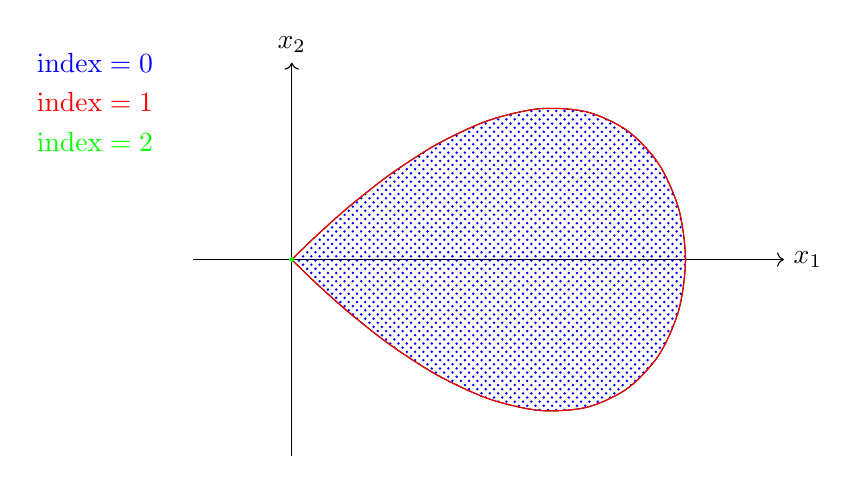
\begin{tikzpicture}[scale=2.5]
  %axes
  \draw[->] (-0.5,0) -- (2.5,0) node[right] {$x_{1}$};
  \draw[->] (0,-1) -- (0,1) node[above] {$x_{2}$};

  %main
  \draw[pattern=crosshatch dots,pattern color=blue,domain=0:2*pi,smooth,variable=\x] plot (-{cos(\x r)+1},{sin(\x r)*sin(\x/2 r)});

  %edge
  \draw[red,domain=0:2*pi,smooth,variable=\x] plot (-{cos(\x r)+1},{sin(\x r)*sin(\x/2 r)});

  %corner
  \filldraw[green] (0,0) circle (0.1mm);

  %labels
  \node[at={(-1,1)},fill=white,text=blue]{$\mathrm{index} = 0$};
  \node[at={(-1,0.8)},fill=white,text=red]{$\mathrm{index} = 1$};
  \node[at={(-1,0.6)},fill=white,text=green]{$\mathrm{index} = 2$};
\end{tikzpicture}
\caption{The teardrop as a manifold with corners but not with faces}
\label{fig:teardrop}
\end{figure}
\\
\end{exa}
\begin{prf}
The technical details are left to the reader.
\\
\phantom{proven}
\hfill
$\Box$
\end{prf}
To describe higher cobordisms we equip manifolds with faces with additional structure. Let $m \in \mathbb{N}$, then an \textbf{$n$-dimensional $\Braket{m}$-manifold} is a pair $(M,(\partial_{0}M,\ldots,\partial_{m-1}M))$ consisting of an $n$-manifold with faces $M$ together with an ordered $m$-tuple $(\partial_{0}M,\ldots,\partial_{m-1}M)$ of faces of $M$ satisfying
\begin{enumerate}
\item[(i)]
$\partial_{0}M \cup \ldots \cup \partial_{m-1}M = \partial M$

\item[(ii)]
$\partial_{i}M \cap \partial_{j}M$ is a (possibly empty) face of both $\partial_{i}M$ and $\partial_{j}M$ for every $0 \leq i \neq j \leq m-1$
\end{enumerate}
We will often simply write $M$ and suppress the $m$-tuple of faces in the notation. Note that a $\Braket{0}$-manifold is just a manifold without boundary, yet the case of dimension $n=0$ is excluded here as we have required manifolds with corners to be at least $1$-dimensional. A $\Braket{1}$-manifold is just a manifold with boundary. 
\\
\begin{exa}
\label{exa:manfaces}
We consider some easy examples.
\begin{enumerate}
\item[(a)]
The space $\mathbb{R}_{n+}^{n}$ is an $n$-manifold with faces whose connected faces are the coordinate hyperplanes defined by $x_{k} = 0$ for $1 \leq k \leq n$. Order these hyperplanes as $H_{1},\ldots,H_{n}$ then $\mathbb{R}_{n+}^{n}$ becomes an $n$-dimensional $\Braket{n}$-manifold by taking $\partial_{k-1}\mathbb{R}_{n+}^{n} = H_{k}$ for $1 \leq k \leq n$ because $H_{i} \cap H_{j}$ is the face of both $H_{i}$ and of $H_{j}$ defined by $x_{i} = 0\ \land\ x_{j} = 0$.

\item[(b)]
The cylindrical shell
\begin{align*}
  C
  &=
  \lbrace
    (x_{1},x_{2},x_{3})
    \in
    \mathbb{R}^{3}
    \colon
    0.5
    \leq
    x_{1}^{2}
    +
    x_{2}^{2}
    \leq
    1
    \ 
    \land
    \ 
    0
    \leq
    x_{3}
    \leq
    1
  \rbrace
\end{align*}
is a $3$-manifold with faces whose connected faces are the top locus defined by $x_{3} = 1$, the bottom locus defined by $x_{3} = 0$, the inner lateral surface defined by $x_{1}^{2} + x_{2}^{2} = 0.5$ and the outer lateral surface defined by $x_{1}^{2} + x_{2}^{2} = 1$. Letting $\partial_{0}C$ the disjoint union of the top and bottom locus and $\partial_{1}C$ the disjoint union of the inner and outer lateral surface, we obtain the structure of a $3$-dimensional $\Braket{2}$-manifold. $\partial_{0}C \cap \partial_{1}C$ is the disjoint union of the circles limiting the top locus and the circles limiting the bottom locus which together constitute a face of both $\partial_{0}C$ and $\partial_{1}C$. For an illustration see figure \ref{fig:cylshell}.
\\
\begin{figure}[h!]
\centering
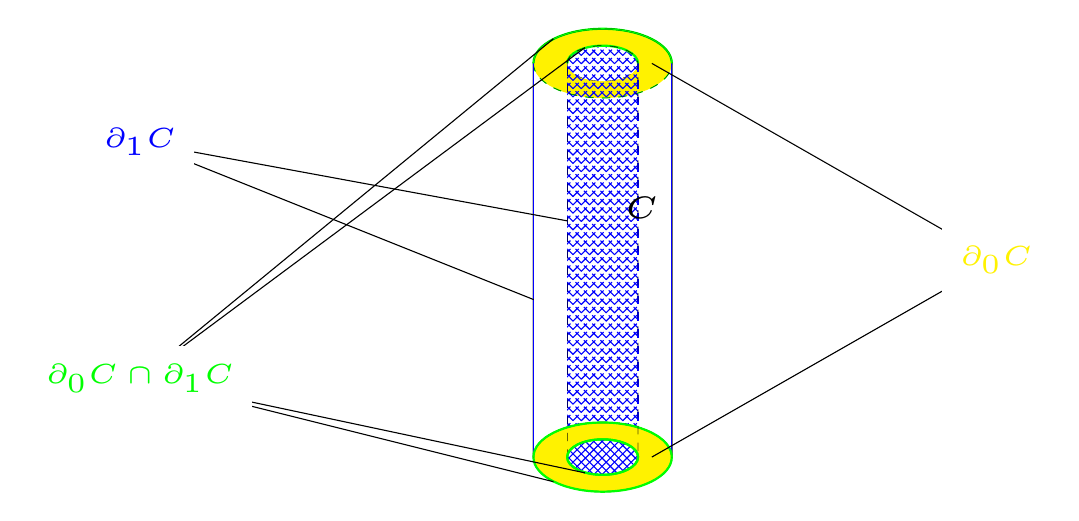
\begin{tikzpicture}[tqft/cobordism/.style={draw},scale=2.5,every node/.style={transform shape}]
  %outer cylinder
  \pic[tqft/cylinder,name=c,every incoming upper boundary component/.style={draw,thick,green},every incoming lower boundary component/.style={draw,dashed,green},every incoming boundary component/.style={fill=yellow}];
  
  %inner cylinder
  \pic[tqft/cylinder,name=c2,every incoming boundary component/.style={draw,ultra thin,dashed,fill=white},every incoming lower boundary component/.style={dashed,green},every incoming upper boundary component/.style={draw,thick,green},cobordism/.style={draw,ultra thin,dashed},cobordism edge/.style={draw,dashed,blue},cobordism outer path/.style={pattern=crosshatch,pattern color=blue},circle x radius=1.8mm,circle y radius=0.9mm];
  
  %redraw outer cylinder
  \pic[tqft/cylinder,every incoming upper boundary component/.style={draw,green},every incoming lower boundary component/.style={draw,ultra thin,dashed},every outgoing boundary component/.style={draw,fill=yellow},cobordism edge/.style={draw,blue},every outgoing lower boundary component/.style={draw,thick,green},every outgoing upper boundary component/.style={draw,thick,green}];
  
  %redraw inner cylinder
  \pic[tqft/cylinder,every incoming boundary component/.style={ultra thin},cobordism/.style={draw,ultra thin,dashed},every outgoing boundary component/.style={draw,fill=white},every outgoing lower boundary component/.style={draw,thick,green},every outgoing upper boundary component/.style={draw,thick,green},circle x radius=1.8mm,circle y radius=0.9mm];
  %re-redraw inner cylinder
  \pic[tqft/cylinder,every incoming boundary component/.style={ultra thin},cobordism/.style={draw,ultra thin,dashed},every outgoing boundary component/.style={pattern=crosshatch,pattern color=blue},every outgoing lower boundary component/.style={draw,thick,green},every outgoing upper boundary component/.style={draw,thick,green},circle x radius=1.8mm,circle y radius=0.9mm];
  
  %labels
  \node[at=(c-between first incoming and first outgoing),right=5.5mm,above=1mm,scale=0.9]{\tiny $C$};
  \draw (0.25,0) -- (2,-1);
  \draw (0.25,-2) -- (2,-1);
  \node[at={(2,-1)},fill=white,text=yellow,scale=0.8]{\tiny $\partial_{0}C$};
  \draw (-0.35,-1.2) -- (-2.35,-0.4);
  \draw (-0.18,-0.8) -- (-2.35,-0.4);
  \node[at={(-2.35,-0.4)},fill=white,text=blue,scale=0.8]{\tiny $\partial_{1}C$};
  \draw (-0.25,0.125) -- (-2.35,-1.6);
  \draw (-0.09,0.08) -- (-2.35,-1.6);
  \draw (-0.25,-2.125) -- (-2.35,-1.6);
  \draw (-0.09,-2.08) -- (-2.35,-1.6);
  \node[at={(-2.35,-1.6)},fill=white,text=green,scale=0.8]{\tiny $\partial_{0}C \cap \partial_{1}C$};
\end{tikzpicture}
\caption{Illustration of a cylindrical shell}
\label{fig:cylshell}
\end{figure}
\\

\item[(c)]
The hexagon $H$ as illustrated in figure \ref{fig:hexagon} is a $2$-dimensional $\Braket{3}$-manifold when taking the disjoint union of the respective opposite edges as the faces $\partial_{0}H$, $\partial_{1}H$ and $\partial_{2}H$ respectively. The intersection $\partial_{i}H \cap \partial_{j}H$, $0 \leq i \neq j \leq 2$ is the disjoint union of the two opposite corners between the respective edges of $\partial_{i}H$ and $\partial_{j}H$ and as each corner is a connected face of each edge, this disjoint union is a face of both $\partial_{i}H$ and $\partial_{j}H$.
\\
\begin{figure}[h!]
\centering
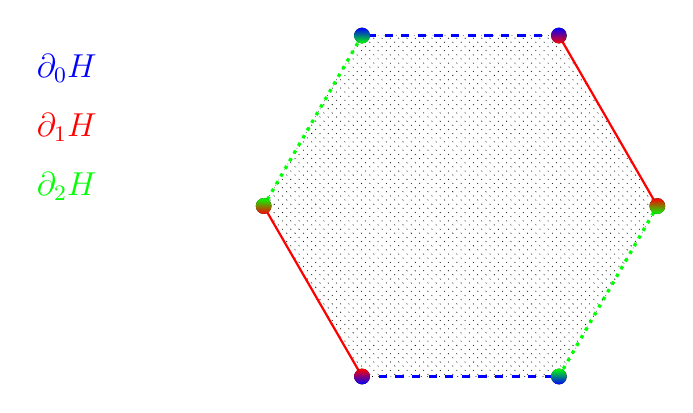
\begin{tikzpicture}[scale=2.5]
  %main
  \draw[pattern=north east lines,very thin,dotted] (0:1) -- (60:1) -- (120:1) -- (180:1) -- (240:1) -- (300:1) -- cycle;

  %model edges
  \draw[red,thick] (0:1) -- (60:1);
  \draw[blue,thick,dashed] (60:1) -- (120:1);
  \draw[green,very thick,dotted] (120:1) -- (180:1);
  \draw[red,thick] (180:1) -- (240:1);
  \draw[blue,thick,dashed] (240:1) -- (300:1);
  \draw[green,very thick,dotted] (300:1) -- (0:1);

  %model corners
  \fill[top color=red,bottom color=green] (0:1) circle (0.4mm);
  \fill[top color=blue,bottom color=red] (60:1) circle (0.4mm);
  \fill[top color=blue,bottom color=green] (120:1) circle (0.4mm);
  \fill[top color=green,bottom color=red] (180:1) circle (0.4mm);
  \fill[top color=red,bottom color=blue] (240:1) circle (0.4mm);
  \fill[top color=green,bottom color=blue] (300:1) circle (0.4mm);

  %labels
  \node[at={(-2,0.7)},fill=white,text=blue]{\large $\partial_{0}H$};
  \node[at={(-2,0.4)},fill=white,text=red]{\large $\partial_{1}H$};
  \node[at={(-2,0.1)},fill=white,text=green]{\large $\partial_{2}H$};
\end{tikzpicture}
\caption{Illustration of the hexagon}
\label{fig:hexagon}
\end{figure}
\\
\end{enumerate}
\end{exa}
\begin{prf}
The technical details are left as an exercise.
\\
\phantom{proven}
\hfill
$\Box$
\end{prf}
Now we come to the definition of higher cobordisms. We take them as unoriented here but the oriented case can be adapted as in the case of ordinary cobordisms. First, for $n \in \mathbb{N}$ we define an \textbf{$n$-dimensional cubical $0$-cobordism} to be a closed $n$-manifold. Now for $n \geq 1$ and $k \in \mathbb{N}^{\times}$ an \textbf{$n$-dimensional cubical $k$-cobordism} is a pair consisting of a compact $n$-dimensional $\Braket{k}$-manifold $(M,(\partial_{0}M,\ldots,\partial_{k-1}M))$ together with a $k$-tuple of decompositions
\begin{align*}
  \partial_{i}M
  &=
  \partial_{i}^{\mathrm{in}}M
  \sqcup
  \partial_{i}^{\mathrm{out}}M
  ,\qquad
  0
  \leq
  i
  \leq
  k-1
\end{align*}
such that $\partial_{i}^{\mathrm{in}}M$ and $\partial_{i}^{\mathrm{out}}M$ are $(n-1)$-dimensional cubical $(k-1)$-cobordisms and
\begin{align*}
  \partial_{j-1}^{\alpha}
  \left(
    \partial_{i}^{\beta}M
  \right)
  &=
  \partial_{i}^{\beta}
  \left(
    \partial_{j}^{\alpha}M
  \right)
  \qquad
  \text{for}
  \qquad
  0
  \leq
  i
  <
  j
  \leq
  k-1
  ,\quad
  \alpha
  ,
  \beta
  \in
  \lbrace
    \mathrm{in}
    ,
    \mathrm{out}
  \rbrace
\end{align*}
as subsets of $M$. The latter condition ensures that the cobordisms are {\glqq}cubical{\grqq} in the sense that the edges of the different faces are joined together as in cubes. Note that for an $n$-dimensional cubical $k$-cobordism it is necessarily the case that $k \leq n$ as there are no $0$-dimensional cubical $k$-cobordisms for $k > 0$. Again, we will frequently abuse notation and supress the faces and their decompositions when giving an $n$-dimensional cubical $k$-cobordism a name. Further, we need a notion of diffeomorphism between such cubical $k$-cobordisms which respects the boundary structure. A \textbf{diffeomorphism rel boundary of $n$-dimensional cubical $k$-cobordisms} $M$ and $\tilde{M}$ is a diffeomorphism of the underlying manifolds with corners which restricts to diffeomorphisms rel boundary of $(n-1)$-dimensional cubical $(k-1)$-cobordisms
\begin{align*}
  \partial_{i}^{\alpha}
  M
  &\to
  \partial_{i}^{\alpha}
  \tilde{M}
  \qquad
  \text{for}
  \qquad
  0
  \leq
  i
  \leq
  k-1
  ,\quad
  \alpha
  \in
  \lbrace
    \mathrm{in}
    ,
    \mathrm{out}
  \rbrace
\end{align*}
\\
\begin{exa}
\label{exa:cubcob}
We consider two examples.
\begin{enumerate}
\item[(a)]
For $k \in \mathbb{N}$ the $k$-cube $I^{k} = [0,1]^{k}$ is a $k$-dimensional cubical $k$-cobordism with
\begin{align*}
  \partial_{i}^{\mathrm{in}}
  I^{k}
  &=
  [0,1]^{i}
  \times
  \lbrace
    1
  \rbrace
  \times
  [0,1]^{k-i-1}
  \qquad
  \text{and}
  \qquad
  \partial_{i}^{\mathrm{out}}
  I^{k}
  =
  [0,1]^{i}
  \times
  \lbrace
    0
  \rbrace
  \times
  [0,1]^{k-i-1}
\end{align*}
for $0 \leq i \leq k-1$. For an illustration in the case $k=3$ see figure \ref{fig:3-cube}.
\\
\begin{figure}[h!]
\centering
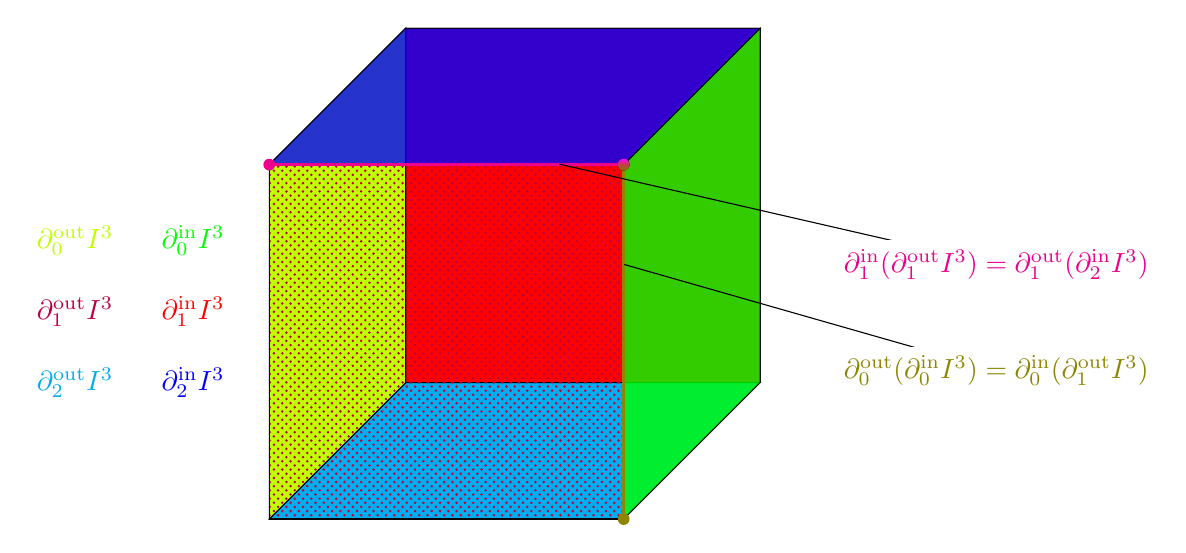
\begin{tikzpicture}[scale=1.5]
  %coordinates
  \coordinate (O) at (0,0,3);
  \coordinate (A) at (0,3,3);
  \coordinate (B) at (0,3,0);
  \coordinate (C) at (0,0,0);
  \coordinate (D) at (3,0,0);
  \coordinate (E) at (3,3,0);
  \coordinate (F) at (3,3,3);
  \coordinate (G) at (3,0,3);
  
  %faces
  \draw[fill=cyan] (C) -- (O) -- (G) -- (D) -- cycle;
  \draw[fill=red] (C) -- (B) -- (E) -- (D) -- cycle;
  \draw[fill=lime] (C) -- (B) -- (A) -- (O) -- cycle;
  \draw[fill=green,opacity=0.8] (D) -- (E) -- (F) -- (G) -- cycle;
  \draw[pattern=crosshatch dots,pattern color=purple] (O) -- (A) -- (F) -- (G) -- cycle;
  \draw[fill=blue,opacity=0.8] (B) -- (A) -- (F) -- (E) -- cycle;

  %coloring edges
  \draw[very thick,magenta] (A) -- (F);
  \draw[very thick,olive] (F) -- (G);

  %coloring corners
  \fill[magenta] (A) circle (0.5mm);
  \fill[top color=magenta,bottom color=olive] (F) circle (0.5mm);
  \fill[olive] (G) circle (0.5mm);

  %face labels
  \node[at={(-1.8,1.2)},fill=white,text=green]{$\partial_{0}^{\mathrm{in}}I^{3}$};
  \node[at={(-1.8,0.6)},fill=white,text=red]{$\partial_{1}^{\mathrm{in}}I^{3}$};
  \node[at={(-1.8,0)},fill=white,text=blue]{$\partial_{2}^{\mathrm{in}}I^{3}$};
  \node[at={(-2.8,1.2)},fill=white,text=lime]{$\partial_{0}^{\mathrm{out}}I^{3}$};
  \node[at={(-2.8,0.6)},fill=white,text=purple]{$\partial_{1}^{\mathrm{out}}I^{3}$};
  \node[at={(-2.8,0)},fill=white,text=cyan]{$\partial_{2}^{\mathrm{out}}I^{3}$};

  %edge labels
  \draw (1.3,1.85) -- (5,1);
  \node[at={(5,1)},fill=white,text=magenta]{$\partial_{1}^{\mathrm{in}}(\partial_{1}^{\mathrm{out}}I^{3}) = \partial_{1}^{\mathrm{out}}(\partial_{2}^{\mathrm{in}}I^{3})$};
  \draw (1.85,1) -- (5,0.1);
  \node[at={(5,0.1)},fill=white,text=olive]{$\partial_{0}^{\mathrm{out}}(\partial_{0}^{\mathrm{in}}I^{3}) = \partial_{0}^{\mathrm{in}}(\partial_{1}^{\mathrm{out}}I^{3})$};
\end{tikzpicture}
\caption{Illustration of the $3$-dimensional cube}
\label{fig:3-cube}
\end{figure}
\\

\item[(b)]
For $n,k \in \mathbb{N}^{\times}$, given an $(n-1)$-dimensional cubical $(k-1)$-cobordism $M$, then $\hat{M} := M \times [0,1]$ is an $n$-dimensional cubical $k$-cobordism with
\begin{align*}
  \partial_{k-1}^{\mathrm{in}}
  \hat{M}
  &=
  M
  \times
  \lbrace
    1
  \rbrace
  \qquad
  \text{and}
  \qquad
  \partial_{k-1}^{\mathrm{out}}
  \hat{M}
  =
  M
  \times
  \lbrace
    0
  \rbrace
\end{align*}
and
\begin{align*}
  \partial_{i}^{\mathrm{in}}
  \hat{M}
  &=
  \partial_{i}^{\mathrm{in}}
  M
  \times
  [0,1]
  \qquad
  \text{and}
  \qquad
  \partial_{i}^{\mathrm{out}}
  \hat{M}
  =
  \partial_{i}^{\mathrm{out}}
  M
  \times
  [0,1]
\end{align*}
for $0 \leq i \leq k-2$.
\\
This procedure can be iterated to obtain an $n$-dimensional cubical $k$-cobordism $M \times [0,1]^{m}$ from a given $(n-m)$-dimensional cubical $(k-m)$-cobordism $M$ for $m \leq k$.
\end{enumerate}
\end{exa}
\begin{prf}
The details are left as an exercise for the diligent reader.
\\
\phantom{proven}
\hfill
$\Box$
\end{prf}
Finally, we want higher cobordisms to go between lower ones with the same source and target and we encode this by demanding increasing triviality for lower faces. For $n,k \in \mathbb{N}$ an \textbf{$n$-dimensional $k$-cobordism} is a triple consisting of an $n$-dimensional cubical $k$-cobordism $M$, of a $k$-tuple of pairs
\begin{align*}
  \left(
    \left(
      M_{0}^{\mathrm{in}}
      ,
      M_{0}^{\mathrm{out}}
    \right)
    ,
    \ldots
    ,
    \left(
      M_{k-1}^{\mathrm{in}}
      ,
      M_{k-1}^{\mathrm{out}}
    \right)
  \right)
\end{align*}
where $M_{i}^{\mathrm{in}}$ and $M_{i}^{\mathrm{out}}$ are $(n-k+i)$-dimensional $i$-cobordisms for $0 \leq i \leq k-1$, called the \textbf{$i$-source} and \textbf{$i$-target}, and of a $k$-tuple of pairs
\begin{align*}
  \left(
    \left(
      f_{0}^{\mathrm{in}}
      ,
      f_{0}^{\mathrm{out}}
    \right)
    ,
    \ldots
    ,
    \left(
      f_{k-1}^{\mathrm{in}}
      ,
      f_{k-1}^{\mathrm{out}}
    \right)
  \right)
\end{align*}
where $f_{i}^{\mathrm{in}}$ and $f_{i}^{\mathrm{out}}$ are diffeomorphisms rel boundary of $(n-1)$-dimensional cubical $(k-1)$-cobordisms
\begin{align*}
  f_{i}^{\mathrm{in}}
  \colon
  \partial_{i}^{\mathrm{in}}M
  \to
  M_{i}^{\mathrm{in}}
  \times
  [0,1]^{k-1-i}
  \qquad
  \text{and}
  \qquad
  f_{i}^{\mathrm{out}}
  \colon
  \partial_{i}^{\mathrm{out}}M
  \to
  M_{i}^{\mathrm{out}}
  \times
  [0,1]^{k-1-i}
\end{align*}
for $0 \leq i \leq k-1$, called the the \textbf{$i$-source map} and \textbf{$i$-target map}, such that the following diagrams commute
\begin{equation*}
\begin{tikzcd}[row sep=3.2em,column sep=4.2em]
  \partial_{j}^{\alpha}
  M_{k-1}^{\beta}
  \ar{r}{(f_{M_{k-1}^{\beta}})_{j}^{\alpha}}
  \ar{d}[swap]{(f_{k-1}^{\beta})^{-1}}
  &
  M_{j}^{\alpha}
  \times
  [0,1]^{k-2-j}
  \\
  \partial_{j}^{\alpha}
  \partial_{k-1}^{\beta}
  M
  \ar{r}{f_{j}^{\alpha}}
  \ar[equals]{d}
  &
  M_{j}^{\alpha}
  \times
  [0,1]^{k-2-j}
  \times
  \lbrace
    \gamma
  \rbrace
  \ar{u}[swap]{\sim_{j}^{\alpha,\gamma}}
  \\
  \partial_{k-2}^{\beta}
  \partial_{j}^{\alpha}
  M
  \ar{ur}[swap]{f_{j}^{\alpha}}
  &
\end{tikzcd}
  \qquad
  \begin{aligned}
    &
    0
    \leq
    j
    \leq
    k-2
    \\
    &
    \alpha
    ,
    \beta
    \in
    \lbrace
      \mathrm{in}
      ,
      \mathrm{out}
    \rbrace
  \end{aligned}
  \quad
  \text{with}
  \quad
  \begin{cases}
    \beta
    =
    \mathrm{in}
    \ 
    \Rightarrow
    \ 
    \gamma
    =
    1
    \\
    \beta
    =
    \mathrm{out}
    \ 
    \Rightarrow
    \ 
    \gamma
    =
    0
  \end{cases}
\end{equation*}
where $(f_{M_{k-1}^{\beta}})_{j}^{\alpha}$ is the $j$-source/target\footnote{depending on whether $\alpha = \mathrm{in}$ or $\alpha = \mathrm{out}$} map of $M_{k-1}^{\beta}$ and $\sim_{j}^{\alpha,\gamma}$ is the obvious identification. Note that all the maps here are diffeomorphisms rel boundary as the restrictions of diffeomorphisms rel boundary to the specified faces are required to be again diffeomorphisms rel boundary. This latter, admittedly somewhat difficult-looking, condition in the definition ensures the compatibility of the sources and targets and implies in particular that the $j$-source/target of the $(k-1)$-source $M_{k-1}^{\mathrm{in}}$ and of the $(k-1)$-target $M_{k-1}^{\mathrm{out}}$ of $M$ coincide with the $j$-source/target of $M$ itself for $0 \leq j \leq k-2$. This hopefully becomes clear in example \ref{exa:saddle} below.
\\
We call the $i$-source and $i$-target the \textbf{$i$-boundaries} and the $i$-source map and the $i$-target map the \textbf{$i$-boundary maps} of the $n$-dimensional $k$-cobordism $M$. Note that a $0$-cobordism is just a cubical $0$-cobordism, i.e. a closed manifold and a $1$-cobordism is nothing but an ordinary (unoriented) cobordism, yet with boundary maps going in the other direction. But the direction of the boundary maps does not matter, of course, since they are diffeomorphisms anyway.
\\
Now a diffeomorphism between $k$-cobordisms should be compatible with the boundary maps. Thus, a \textbf{diffeomorphism rel boundary of $n$-dimensional $k$-cobordisms} $M,\tilde{M}$ with the same sources and targets, call it $g \colon M \to \tilde{M}$, is a diffeomorphism rel boundary of the underlying $n$-dimensional cubical $k$-cobordisms which is compatible with the boundary maps in the sense that
\begin{align*}
  \tilde{f}_{i}^{\alpha}
  \circ
  g
  \vert
  \partial_{i}^{\alpha}
  M
  &=
  f_{i}^{\alpha}
  \qquad
  \text{for}
  \qquad
  0
  \leq
  i
  \leq
  k-1
  ,\quad
  \alpha
  \in
  \lbrace
    \mathrm{in}
    ,
    \mathrm{out}
  \rbrace
\end{align*}
Just as in the case of ordinary cobordisms we say that two $n$-dimensional $k$-cobordisms are \textbf{equivalent} if there is a diffeomorphism rel boundary between them.
\\
\begin{exa}
\label{exa:saddle}
As an example for a $2$-dimensional $2$-cobordism consider the {\glqq}saddle{\grqq} as illustrated in figure \ref{fig:saddle}, denoted $N$. Note that the compatibility of the boundaries requires for example that
\begin{equation*}
\begin{tikzcd}[row sep=3.2em,column sep=4.2em]
  \partial_{0}^{\mathrm{out}}
  N_{1}^{\mathrm{in}}
  \ar{r}{(f_{N_{1}^{\mathrm{in}}})_{0}^{\mathrm{out}}}
  \ar{d}[swap]{(f_{1}^{\mathrm{in}})^{-1}}
  &
  N_{0}^{\mathrm{out}}
  \\
  \partial_{0}^{\mathrm{out}}
  \partial_{1}^{\mathrm{in}}
  N
  \ar{r}{f_{0}^{\mathrm{out}}}
  \ar[equals]{d}
  &
  N_{0}^{\mathrm{out}}
  \times
  \lbrace
    1
  \rbrace
  \ar{u}[swap]{\sim_{0}^{\mathrm{out},1}}
  \\
  \partial_{0}^{\mathrm{in}}
  \partial_{0}^{\mathrm{out}}
  N
  \ar{ur}[swap]{f_{0}^{\mathrm{out}}}
  &
\end{tikzcd}
\end{equation*}
commutes, and similarly for the other boundary maps.
\\
\begin{figure}[h!]
\centering
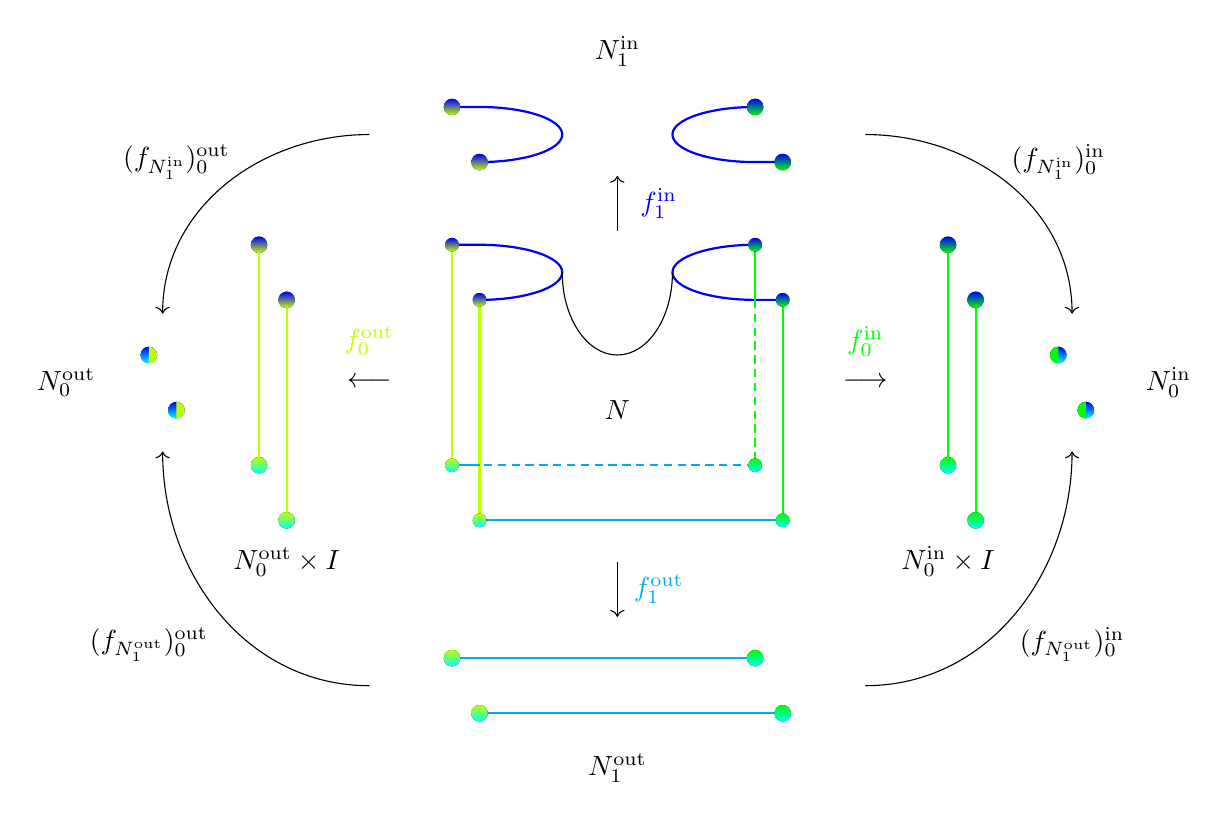
\begin{tikzpicture}[scale=3.5,thick]
  % top
  %edges
  \draw[blue] (1,3.5) arc (90:270:0.3cm and 0.1cm) -- (1.1,3.3);
  \draw[blue] (-0.1,3.5) -- (0,3.5) arc (90:-90:0.3cm and 0.1cm);
  %corners
  \fill[top color=blue,bottom color=green] (1,3.5) circle (0.3mm);
  \fill[top color=blue,bottom color=green] (1.1,3.3) circle (0.3mm);
  \fill[top color=blue,bottom color=lime] (-0.1,3.5) circle (0.3mm);
  \fill[top color=blue,bottom color=lime] (0,3.3) circle (0.3mm);
  %labels
  \node[at={(0.5,3.7)}]{$N_{1}^{\mathrm{in}}$};
  \draw[thin,->] (0.5,3.05) -- (0.5,3.25);
  \node[at={(0.65,3.15)},text=blue]{$f_{1}^{\mathrm{in}}$};
  
  % main
  %edges
  \draw[blue] (-0.1,3) -- (0,3) arc (90:-90:0.3cm and 0.1cm);
  \draw[blue] (1,3) arc (90:270:0.3cm and 0.1cm) -- (1.1,2.8);
  \draw[lime] (0,2.8) -- (0,2);
  \draw[lime] (-0.1,3) -- (-0.1,2.2);
  \draw[green] (1.1,2.8) -- (1.1,2);
  \draw[green] (1,3) -- (1,2.8);
  \draw[green,densely dashed] (1,2.8) -- (1,2.2);
  \draw[cyan,densely dashed] (1,2.2) -- (0,2.2);
  \draw[cyan] (1.1,2) -- (0,2);
  \draw[cyan] (-0.1,2.2) -- (0,2.2);
  \draw[thin] (0.3,2.9) arc (180:360:0.2cm and 0.3cm);
  %corners
  \fill[top color=blue,bottom color=green] (1,3) circle (0.25mm);
  \fill[top color=blue,bottom color=green] (1.1,2.8) circle (0.25mm);
  \fill[top color=blue,bottom color=lime] (-0.1,3) circle (0.25mm);
  \fill[top color=blue,bottom color=lime] (0,2.8) circle (0.25mm);
  \fill[top color=green,bottom color=cyan] (1,2.2) circle (0.25mm);
  \fill[top color=green,bottom color=cyan] (1.1,2) circle (0.25mm);
  \fill[top color=lime,bottom color=cyan] (-0.1,2.2) circle (0.25mm);
  \fill[top color=lime,bottom color=cyan] (0,2) circle (0.25mm);
  %labels
  \node[at={(0.5,2.4)}]{$N$};
  
  % bottom
  %edges
  \draw[cyan] (-0.1,1.5) -- (1,1.5) (0,1.3) -- (1.1,1.3);
  %corners
  \fill[top color=lime,bottom color=cyan] (-0.1,1.5) circle (0.3mm);
  \fill[top color=lime,bottom color=cyan] (0,1.3) circle (0.3mm);
  \fill[top color=green,bottom color=cyan] (1,1.5) circle (0.3mm);
  \fill[top color=green,bottom color=cyan] (1.1,1.3) circle (0.3mm);
  %labels
  \node[at={(0.5,1.1)}]{$N_{1}^{\mathrm{out}}$};
  \draw[thin,<-] (0.5,1.65) -- (0.5,1.85);
  \node[at={(0.65,1.75)},text=cyan]{$f_{1}^{\mathrm{out}}$};
  
  % left
  %edges
  \draw[lime] (-0.7,2.8) -- (-0.7,2) (-0.8,3) -- (-0.8,2.2);
  %corners
  \fill[top color=blue,bottom color=lime] (-0.7,2.8) circle (0.3mm);
  \fill[top color=blue,bottom color=lime] (-0.8,3) circle (0.3mm);
  \fill[top color=lime,bottom color=cyan] (-0.7,2) circle (0.3mm);
  \fill[top color=lime,bottom color=cyan] (-0.8,2.2) circle (0.3mm);
  \fill[top color=blue,bottom color=cyan] (-1.1,2.4) circle (0.3mm);
  \fill[lime] (-1.1,2.37) arc (270:450:0.3mm);
  \fill[top color=blue,bottom color=cyan] (-1.2,2.6) circle (0.3mm);
  \fill[lime] (-1.2,2.57) arc (270:450:0.3mm);
  %labels
  \node[at={(-1.5,2.5)}]{$N_{0}^{\mathrm{out}}$};
  \node[at={(-0.7,1.85)}]{$N_{0}^{\mathrm{out}} \times I$};
  \node[at={(-0.4,2.65)},text=lime]{$f_{0}^{\mathrm{out}}$};
  \node[at={(-0.4,2.5)}]{$\longleftarrow$};
  \draw[thin,<-] (-1.15,2.75) to [out=90,in=180] (-0.4,3.4);
  \draw[thin,<-] (-1.15,2.25) to [out=270,in=180] (-0.4,1.4);
  \node[at={(-1.1,3.3)}]{$(f_{N_{1}^{\mathrm{in}}})_{0}^{\mathrm{out}}$};
  \node[at={(-1.2,1.55)}]{$(f_{N_{1}^{\mathrm{out}}})_{0}^{\mathrm{out}}$};
  
  % right
  %edges
  \draw[green] (1.8,2.8) -- (1.8,2) (1.7,3) -- (1.7,2.2);
  %corners
  \fill[top color=blue,bottom color=green] (1.8,2.8) circle (0.3mm);
  \fill[top color=blue,bottom color=green] (1.7,3) circle (0.3mm);
  \fill[top color=green,bottom color=cyan] (1.8,2) circle (0.3mm);
  \fill[top color=green,bottom color=cyan] (1.7,2.2) circle (0.3mm);
  \fill[top color=blue,bottom color=cyan] (2.2,2.4) circle (0.3mm);
  \fill[green] (2.2,2.43) arc (90:270:0.3mm);
  \fill[top color=blue,bottom color=cyan] (2.1,2.6) circle (0.3mm);
  \fill[green] (2.1,2.63) arc (90:270:0.3mm);
  %labels
  \node[at={(2.5,2.5)}]{$N_{0}^{\mathrm{in}}$};
  \node[at={(1.7,1.85)}]{$N_{0}^{\mathrm{in}} \times I$};
  \node[at={(1.4,2.65)},text=green]{$f_{0}^{\mathrm{in}}$};
  \node[at={(1.4,2.5)}]{$\longrightarrow$};
  \draw[thin,<-] (2.15,2.75) to [out=90,in=0] (1.4,3.4);
  \draw[thin,<-] (2.15,2.25) to [out=270,in=0] (1.4,1.4);
  \node[at={(2.1,3.3)}]{$(f_{N_{1}^{\mathrm{in}}})_{0}^{\mathrm{in}}$};
  \node[at={(2.15,1.55)}]{$(f_{N_{1}^{\mathrm{out}}})_{0}^{\mathrm{in}}$};
\end{tikzpicture}
\caption{Illustration of the saddle}
\label{fig:saddle}
\end{figure}
\\
\end{exa}
\begin{prf}
Once again, the technical details can be filled in as an exercise.
\\
\phantom{proven}
\hfill
$\Box$
\end{prf}
Remember that given two ordinary $1$-cobordisms $M_{1},M_{2}$ such that the target of $M_{1}$ and the source of $M_{2}$ are the same, then the two can be glued together along the common boundary to yield a new $1$-cobordism with source the source of $M_{1}$ and target the target of $M_{2}$. Similarly, two $k$-cobordisms $M_{1},M_{2}$ can be glued together, but now there are $k$ directions in which one can glue. If the $i$-target of $M_{1}$ and the $i$-source of $M_{2}$ are the same - which implies that the corresponding $j$-boundaries for $j < i$ are the same for $M_{1}$ and $M_{2}$ - then the two $k$-cobordisms can be glued along this common part of the $i$-boundary to yield a new $k$-cobordism and this can be done for $0 \leq i \leq k-1$. The resulting $k$-cobordism has as $i$-source the $i$-source of $M_{1}$ and as $i$-target the $i$-target of $M_{2}$ and hence the same $j$-boundaries as $M_{1}$ and $M_{2}$ for $j < i$. For the other $j > i$ the $j$-source and $j$-target is the gluing of, respectively, the $j$-sources and $j$-targets of $M_{1}$ and $M_{2}$ along their respective common restriction of the $i$-boundary along which $M_{1}$ and $M_{2}$ are glued. This hopefully becomes clear in the following example.
\\
\begin{exa}
\label{exa:gluing}
As an example for gluing higher cobordisms consider the $2$-dimensional $2$-cobordism in figure \ref{fig:halfcyl}, denoted $M$.
\\
\begin{figure}[h!]
\centering
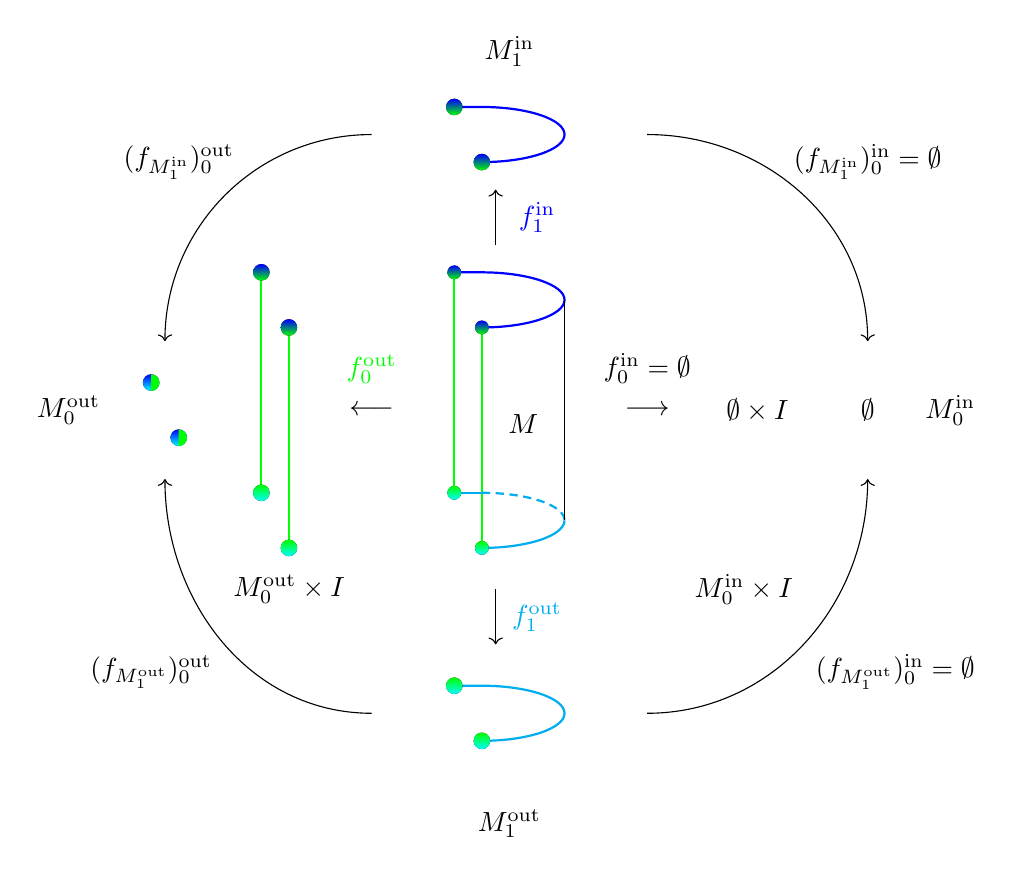
\begin{tikzpicture}[scale=3.5,thick]
  % top
  %edges
  \draw[blue] (-0.1,3.6) -- (0,3.6) arc (90:-90:0.3cm and 0.1cm);
  %corners
  \fill[top color=blue,bottom color=green] (-0.1,3.6) circle (0.3mm);
  \fill[top color=blue,bottom color=green] (0,3.4) circle (0.3mm);
  %labels
  \node[at={(0.1,3.8)}]{$M_{1}^{\mathrm{in}}$};
  \draw[thin,->] (0.05,3.1) -- (0.05,3.3);
  \node[at={(0.2,3.2)},text=blue]{$f_{1}^{\mathrm{in}}$};
  
  % main
  %edges
  \draw[blue] (-0.1,3) -- (0,3) arc (90:-90:0.3cm and 0.1cm);
  \draw[green] (0,2.8) -- (0,2);
  \draw[green] (-0.1,3) -- (-0.1,2.2);
  \draw[cyan] (-0.1,2.2) -- (0,2.2);
  \draw[cyan,densely dashed] (0,2.2) arc (90:0:0.3cm and 0.1cm);
  \draw[cyan] (0.3,2.1) arc (0:-90:0.3cm and 0.1cm);
  \draw[thin] (0.3,2.9) -- (0.3,2.1);
  %corners
  \fill[top color=blue,bottom color=green] (-0.1,3) circle (0.25mm);
  \fill[top color=blue,bottom color=green] (0,2.8) circle (0.25mm);
  \fill[top color=green,bottom color=cyan] (-0.1,2.2) circle (0.25mm);
  \fill[top color=green,bottom color=cyan] (0,2) circle (0.25mm);
  %labels
  \node[at={(0.15,2.45)}]{$M$};
  
  % bottom
  %edges
  \draw[cyan] (-0.1,1.5) -- (0,1.5) arc (90:-90:0.3cm and 0.1cm);
  %corners
  \fill[top color=green,bottom color=cyan] (-0.1,1.5) circle (0.3mm);
  \fill[top color=green,bottom color=cyan] (0,1.3) circle (0.3mm);
  %labels
  \node[at={(0.1,1)}]{$M_{1}^{\mathrm{out}}$};
  \draw[thin,<-] (0.05,1.65) -- (0.05,1.85);
  \node[at={(0.2,1.75)},text=cyan]{$f_{1}^{\mathrm{out}}$};
  
  % left
  %edges
  \draw[green] (-0.7,2.8) -- (-0.7,2) (-0.8,3) -- (-0.8,2.2);
  %corners
  \fill[top color=blue,bottom color=green] (-0.7,2.8) circle (0.3mm);
  \fill[top color=blue,bottom color=green] (-0.8,3) circle (0.3mm);
  \fill[top color=green,bottom color=cyan] (-0.7,2) circle (0.3mm);
  \fill[top color=green,bottom color=cyan] (-0.8,2.2) circle (0.3mm);
  \fill[top color=blue,bottom color=cyan] (-1.1,2.4) circle (0.3mm);
  \fill[green] (-1.1,2.37) arc (270:450:0.3mm);
  \fill[top color=blue,bottom color=cyan] (-1.2,2.6) circle (0.3mm);
  \fill[green] (-1.2,2.57) arc (270:450:0.3mm);
  %labels
  \node[at={(-1.5,2.5)}]{$M_{0}^{\mathrm{out}}$};
  \node[at={(-0.7,1.85)}]{$M_{0}^{\mathrm{out}} \times I$};
  \node[at={(-0.4,2.65)},text=green]{$f_{0}^{\mathrm{out}}$};
  \node[at={(-0.4,2.5)}]{$\longleftarrow$};
  \draw[thin,<-] (-1.15,2.75) to [out=90,in=180] (-0.4,3.5);
  \draw[thin,<-] (-1.15,2.25) to [out=270,in=180] (-0.4,1.4);
  \node[at={(-1.1,3.4)}]{$(f_{M_{1}^{\mathrm{in}}})_{0}^{\mathrm{out}}$};
  \node[at={(-1.2,1.55)}]{$(f_{M_{1}^{\mathrm{out}}})_{0}^{\mathrm{out}}$};
  
  % right
  %edges
  \node[at={(1,2.5)}]{$\emptyset \times I$};
  %corners
  \node[at={(1.4,2.5)}]{$\emptyset$};
  %labels
  \node[at={(1.7,2.5)}]{$M_{0}^{\mathrm{in}}$};
  \node[at={(0.95,1.85)}]{$M_{0}^{\mathrm{in}} \times I$};
  \node[at={(0.6,2.65)}]{$f_{0}^{\mathrm{in}} = \emptyset$};
  \node[at={(0.6,2.5)}]{$\longrightarrow$};
  \draw[thin,<-] (1.4,2.75) to [out=90,in=0] (0.6,3.5);
  \draw[thin,<-] (1.4,2.25) to [out=270,in=0] (0.6,1.4);
  \node[at={(1.4,3.4)}]{$(f_{M_{1}^{\mathrm{in}}})_{0}^{\mathrm{in}} = \emptyset$};
  \node[at={(1.5,1.55)}]{$(f_{M_{1}^{\mathrm{out}}})_{0}^{\mathrm{in}} = \emptyset$};
\end{tikzpicture}
\caption{$2$-cobordism whose $0$-target is the same as the $0$-source of the saddle}
\label{fig:halfcyl}
\end{figure}
\clearpage
Gluing this to the saddle $N$ from example \ref{exa:saddle} along $N_{0}^{\mathrm{in}} = M_{0}^{\mathrm{out}}$ results in the $2$-dimensional $2$-cobordism depicted in figure \ref{fig:glued}.
\\
\begin{figure}[h!]
\centering
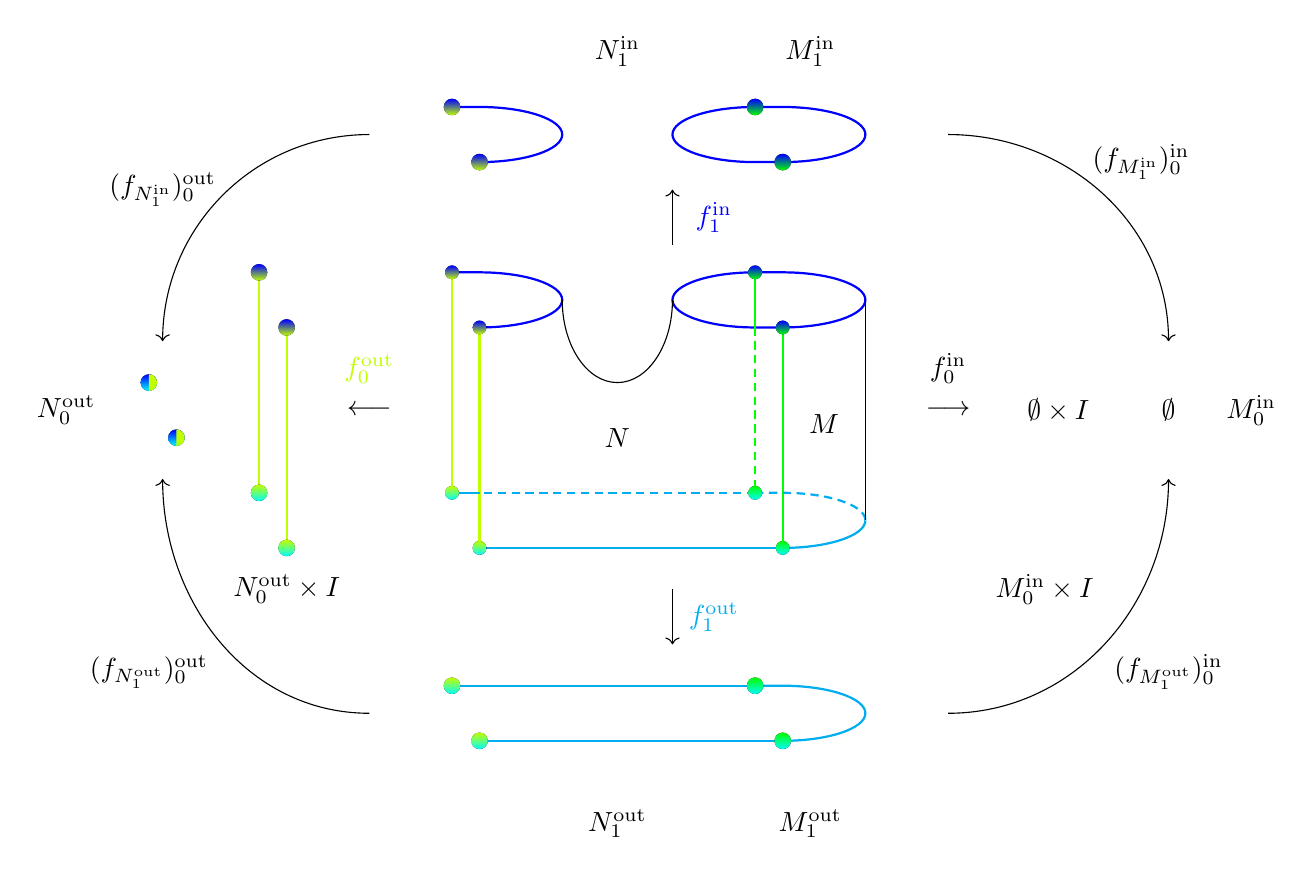
\begin{tikzpicture}[scale=3.5,thick]
  % top
  %edges
  \draw[blue] (1,3.6) arc (90:270:0.3cm and 0.1cm) -- (1.1,3.4);
  \draw[blue] (1,3.6) -- (1.1,3.6) arc (90:-90:0.3cm and 0.1cm);
  \draw[blue] (-0.1,3.6) -- (0,3.6) arc (90:-90:0.3cm and 0.1cm);
  %corners
  \fill[top color=blue,bottom color=green] (1,3.6) circle (0.3mm);
  \fill[top color=blue,bottom color=green] (1.1,3.4) circle (0.3mm);
  \fill[top color=blue,bottom color=lime] (-0.1,3.6) circle (0.3mm);
  \fill[top color=blue,bottom color=lime] (0,3.4) circle (0.3mm);
  %labels
  \node[at={(0.5,3.8)}]{$N_{1}^{\mathrm{in}}$};
  \node[at={(1.2,3.8)}]{$M_{1}^{\mathrm{in}}$};
  \draw[thin,->] (0.7,3.1) -- (0.7,3.3);
  \node[at={(0.85,3.2)},text=blue]{$f_{1}^{\mathrm{in}}$};
  
  % main
  %edges
  \draw[blue] (-0.1,3) -- (0,3) arc (90:-90:0.3cm and 0.1cm);
  \draw[blue] (1,3) arc (90:270:0.3cm and 0.1cm) -- (1.1,2.8);
  \draw[blue] (1,3) -- (1.1,3) arc (90:-90:0.3cm and 0.1cm);
  \draw[lime] (0,2.8) -- (0,2);
  \draw[lime] (-0.1,3) -- (-0.1,2.2);
  \draw[green] (1.1,2.8) -- (1.1,2);
  \draw[green] (1,3) -- (1,2.8);
  \draw[green,densely dashed] (1,2.8) -- (1,2.2);
  \draw[cyan,densely dashed] (1,2.2) -- (0,2.2);
  \draw[cyan] (1.1,2) -- (0,2);
  \draw[cyan] (-0.1,2.2) -- (0,2.2);
  \draw[cyan,densely dashed] (1,2.2) -- (1.1,2.2) arc (90:0:0.3cm and 0.1cm);
  \draw[cyan] (1.4,2.1) arc (0:-90:0.3cm and 0.1cm);
  \draw[thin] (0.3,2.9) arc (180:360:0.2cm and 0.3cm);
  \draw[thin] (1.4,2.9) -- (1.4,2.1);
  %corners
  \fill[top color=blue,bottom color=green] (1,3) circle (0.25mm);
  \fill[top color=blue,bottom color=green] (1.1,2.8) circle (0.25mm);
  \fill[top color=blue,bottom color=lime] (-0.1,3) circle (0.25mm);
  \fill[top color=blue,bottom color=lime] (0,2.8) circle (0.25mm);
  \fill[top color=green,bottom color=cyan] (1,2.2) circle (0.25mm);
  \fill[top color=green,bottom color=cyan] (1.1,2) circle (0.25mm);
  \fill[top color=lime,bottom color=cyan] (-0.1,2.2) circle (0.25mm);
  \fill[top color=lime,bottom color=cyan] (0,2) circle (0.25mm);
  %labels
  \node[at={(0.5,2.4)}]{$N$};
  \node[at={(1.25,2.45)}]{$M$};
  
  % bottom
  %edges
  \draw[cyan] (-0.1,1.5) -- (1,1.5) (0,1.3) -- (1.1,1.3);
  \draw[cyan] (1,1.5) -- (1.1,1.5) arc (90:-90:0.3cm and 0.1cm);
  %corners
  \fill[top color=lime,bottom color=cyan] (-0.1,1.5) circle (0.3mm);
  \fill[top color=lime,bottom color=cyan] (0,1.3) circle (0.3mm);
  \fill[top color=green,bottom color=cyan] (1,1.5) circle (0.3mm);
  \fill[top color=green,bottom color=cyan] (1.1,1.3) circle (0.3mm);
  %labels
  \node[at={(0.5,1)}]{$N_{1}^{\mathrm{out}}$};
  \node[at={(1.2,1)}]{$M_{1}^{\mathrm{out}}$};
  \draw[thin,<-] (0.7,1.65) -- (0.7,1.85);
  \node[at={(0.85,1.75)},text=cyan]{$f_{1}^{\mathrm{out}}$};
  
  % left
  %edges
  \draw[lime] (-0.7,2.8) -- (-0.7,2) (-0.8,3) -- (-0.8,2.2);
  %corners
  \fill[top color=blue,bottom color=lime] (-0.7,2.8) circle (0.3mm);
  \fill[top color=blue,bottom color=lime] (-0.8,3) circle (0.3mm);
  \fill[top color=lime,bottom color=cyan] (-0.7,2) circle (0.3mm);
  \fill[top color=lime,bottom color=cyan] (-0.8,2.2) circle (0.3mm);
  \fill[top color=blue,bottom color=cyan] (-1.1,2.4) circle (0.3mm);
  \fill[lime] (-1.1,2.37) arc (270:450:0.3mm);
  \fill[top color=blue,bottom color=cyan] (-1.2,2.6) circle (0.3mm);
  \fill[lime] (-1.2,2.57) arc (270:450:0.3mm);
  %labels
  \node[at={(-1.5,2.5)}]{$N_{0}^{\mathrm{out}}$};
  \node[at={(-0.7,1.85)}]{$N_{0}^{\mathrm{out}} \times I$};
  \node[at={(-0.4,2.65)},text=lime]{$f_{0}^{\mathrm{out}}$};
  \node[at={(-0.4,2.5)}]{$\longleftarrow$};
  \draw[thin,<-] (-1.15,2.75) to [out=90,in=180] (-0.4,3.5);
  \draw[thin,<-] (-1.15,2.25) to [out=270,in=180] (-0.4,1.4);
  \node[at={(-1.15,3.3)}]{$(f_{N_{1}^{\mathrm{in}}})_{0}^{\mathrm{out}}$};
  \node[at={(-1.2,1.55)}]{$(f_{N_{1}^{\mathrm{out}}})_{0}^{\mathrm{out}}$};
  
  % right
  %edges
  \node[at={(2.1,2.5)}]{$\emptyset \times I$};
  %corners
  \node[at={(2.5,2.5)}]{$\emptyset$};
  %labels
  \node[at={(2.8,2.5)}]{$M_{0}^{\mathrm{in}}$};
  \node[at={(2.05,1.85)}]{$M_{0}^{\mathrm{in}} \times I$};
  \node[at={(1.7,2.65)}]{$f_{0}^{\mathrm{in}}$};
  \node[at={(1.7,2.5)}]{$\longrightarrow$};
  \draw[thin,<-] (2.5,2.75) to [out=90,in=0] (1.7,3.5);
  \draw[thin,<-] (2.5,2.25) to [out=270,in=0] (1.7,1.4);
  \node[at={(2.4,3.4)}]{$(f_{M_{1}^{\mathrm{in}}})_{0}^{\mathrm{in}}$};
  \node[at={(2.5,1.55)}]{$(f_{M_{1}^{\mathrm{out}}})_{0}^{\mathrm{in}}$};
\end{tikzpicture}
\caption{$2$-cobordism obtained by gluing the one from figure \ref{fig:halfcyl} and the saddle}
\label{fig:glued}
\end{figure}
\\
\end{exa}
\begin{prf}
Filling in the technical details can be done as an exercise.
\\
\phantom{proven}
\hfill
$\Box$
\end{prf}
There are several subtleties involved in this process of gluing, some of which are similar to the case of ordinary cobordisms, for example, the gluings of $k$-cobordisms are achieved by choosing appropriate collars, which is always possible. Therefore the resulting $k$-cobordisms obtained by gluing are well-defined only up to equivalence of $k$-cobordisms. We will not press the details further here and refer the interested reader to \cite{d37d0fca} instead where the $2$-dimensional case is treated extensively and illustrates all the details.




\chapter{Motivation: Low-Dimensional TQFTs}
\label{chap:lowdimtqft}
\stepcounter{prpcounter}
We now start to work out the structure of low dimensional ordinary TQFTs to get an idea of how a classification might look in general. To this end we return to oriented cobordisms for the next sections. We start with $1$-dimensional TQFTs in section \ref{sec:1dimtqft} which are particularly easy to classify. In section \ref{sec:2dimtqft} we then consider $2$-dimensional TQFTs for which an explicit classification in terms of algebraic objects is still not too difficult but already involves much more data.



\section{1-Dimensional TQFTs}
\label{sec:1dimtqft}
%\nocite{0a816f4c}
%%%
For a 1-dimensional ordinary TQFT
\begin{align*}
  Z
  \colon
  \mathbf{Cob}_{1}
  &\to
  \mathbf{Vec}_{K}
\end{align*}
we have a finite-dimensional vector space $Z(S)$ associated to every closed oriented $0$-manifold $S \in \mathrm{ob}_{\mathbf{Cob}_{1}}$. Such a manifold is a finite set of points, where each point has a positive or negative orientation, so that we can consider the manifold as a disjoint union of positive points and of negative points, as there always is an orientation-preserving diffeomorphism\footnote{remember that an orientation-preserving diffeomorphism induces an isomorphism in the cobordism category via the cylinder construction} to such a disjoint union. This means that there are two points (at least up to orientation-preserving diffeomorphism), the positively oriented point $\bullet_{+}$ and the negatively oriented point $\bullet_{-} = \overline{\bullet_{+}}$, that build up all objects in $\mathbf{Cob}_{1}$ by disjoint union. Hence, for $S$ we can write
\begin{align*}
  S
  &\cong
  \bullet_{+}^{\sqcup k}
  \sqcup
  \bullet_{-}^{\sqcup m}
\end{align*}
for some $k,m \in \mathbb{N}$, where the superscript $\sqcup k$ means $k$-fold disjoint union. The TQFT $Z$ assigns a finite-dimensional vector space to each of these points, yet, as $\bullet_{-}$ is a dual object of $\bullet_{+}$ we know that $Z(\bullet_{-})$ is canonically isomorphic to the dual space $V^{\prime}$ of $Z(\bullet_{+}) =: V$. Moreover, as $Z$ is a symmetric monoidal functor, $Z(S)$ is canonically isomorphic\footnote{by the natural isomorphism that is part of the symmetric monoidal functor which we did not make explicit here; we did not make explicit the isomorphism for the unit objects either but both will be tacitly used here for identifications} to
\begin{align*}
  V^{\otimes k}
  \otimes
  (V^{\prime})^{\otimes m}
\end{align*}
where the superscript $\otimes k$ means $k$-fold tensor product. From this we see that $Z$ is determined on objects by only one datum, namely the finite-dimensional vector space associated to the positively oriented\footnote{this is just a matter of convention, as there is certainly no reason to prefer the positive orientation, and we might equivalently choose the negatively oriented point} point.
\\
Now what happens on the level of morphisms? As $Z$ is symmetric monoidal, disjoint unions are basically taken to tensor products on the morphism level, too, so that it suffices to consider connected cobordism classes. A connected smooth compact 1-manifold with boundary is either diffeomorphic to the closed interval $[0,1]$ or to the circle $S^{1}$ but we also have to take orientations and in- and out-boundaries into account. For the circle this does not matter as there are no boundaries and there is an orientation-reversing diffeomorphism for the circle (a reflection), i.e. the circle with the opposite orientation represents the same morphism as with the original orientation. For the closed interval $[0,1]$ there are different cases to consider:
\begin{enumerate}
\item[i)]
The interval $M = [0,1]$ can represent the identity for $\bullet_{+}$ or $\bullet_{-}$, that is $\mathrm{id}_{\bullet_{+}}$ or $\mathrm{id}_{\bullet_{-}}$ as pictured below (remember we depict cobordisms from top down).
\begin{equation*}
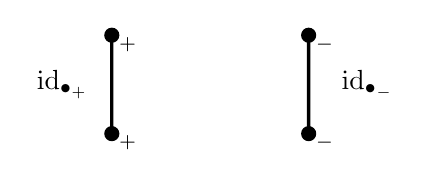
\begin{tikzpicture}[scale=1.25,very thick]
  \filldraw
    (0,0) circle (1.7pt) node[shift={(0.2,-0.12)}] {\scriptsize{$+$}}
    --
    (0,1) circle (1.7pt) node[shift={(0.2,-0.12)}] {\scriptsize{$+$}};
  \filldraw
    (2,0) circle (1.7pt) node[shift={(0.2,-0.12)}] {\scriptsize{$-$}}
    --
    (2,1) circle (1.7pt) node[shift={(0.2,-0.12)}] {\scriptsize{$-$}};
  \draw
    (-0.5,0.5) node[fill=white] {$\mathrm{id}_{\bullet_{+}}$}
    (2.6,0.5) node[fill=white] {$\mathrm{id}_{\bullet_{-}}$};
\end{tikzpicture}
\end{equation*}
Since $Z$ is a functor we find in these cases that $Z([M])$ is just $\mathrm{id}_{V}$ or $\mathrm{id}_{V^{\prime}}$

\item[ii)]
The interval $M = [0,1]$ can represent a cobordism from the empty 0-manifold $\emptyset$ to $\bullet_{+} \sqcup \bullet_{-}$, namely the coevaluation $\mathrm{coev}_{\bullet_{+}}$. Analogously, it can represent the coevaluation $\mathrm{coev}_{\bullet_{-}}$ for $\bullet_{-}$.
\begin{equation*}
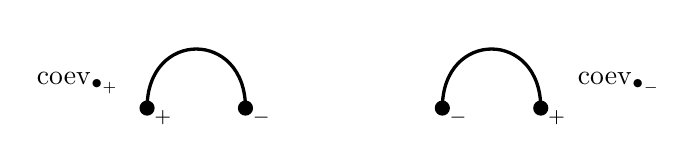
\begin{tikzpicture}[scale=1.25,very thick]
  \filldraw
    (0,0) circle (1.7pt) node[shift={(0.2,-0.12)}] {\scriptsize{$+$}}
    (1,0) circle (1.7pt) node[shift={(0.2,-0.12)}] {\scriptsize{$-$}};
  \draw
    (0,0)
    ..
    controls
    +(0,0.8)
    and
    +(0,0.8)
    ..
    (1,0);
  \filldraw
    (3,0) circle (1.7pt) node[shift={(0.2,-0.12)}] {\scriptsize{$-$}}
    (4,0) circle (1.7pt) node[shift={(0.2,-0.12)}] {\scriptsize{$+$}};
  \draw
    (3,0)
    ..
    controls
    +(0,0.8)
    and
    +(0,0.8)
    ..
    (4,0);
  \draw
    (-0.7,0.25) node[fill=white] {$\mathrm{coev}_{\bullet_{+}}$}
    (4.8,0.25) node[fill=white] {$\mathrm{coev}_{\bullet_{-}}$};
\end{tikzpicture}
\end{equation*}
As $Z$ is monoidal, $Z([M])$ can be identified with the coevaluations for $V$ and $V^{\prime}$ respectively, i.e. for a basis $\lbrace v_{1},\ldots,v_{l} \rbrace$ of $V$ (supposed that the dimension of $V$ is $l \in \mathbb{N}$) and the corresponding dual basis $\lbrace v_{1}^{\prime},\ldots,v_{l}^{\prime} \rbrace$ of $V^{\prime}$ we obtain
\begin{align*}
  \mathrm{coev}_{V}
  \colon
  K
  \to
  V
  \otimes
  V^{\prime}
  ,\qquad
  x
  &\mapsto
  x
  \sum_{i=1}^{l}
  v_{i}
  \otimes
  v_{i}^{\prime}
\end{align*}
or
\begin{align*}
  \mathrm{coev}_{V^{\prime}}
  \colon
  K
  \to
  V^{\prime}
  \otimes
  V
  ,\qquad
  x
  &\mapsto
  x
  \sum_{i=1}^{l}
  v_{i}^{\prime}
  \otimes
  v_{i}
\end{align*}
for $Z([M])$.

\item[iii)]
The interval $M = [0,1]$ can represent a cobordism from $\bullet_{-} \sqcup \bullet_{+}$ to the empty 0-manifold $\emptyset$, namely the evaluation $\mathrm{ev}_{\bullet_{+}}$. Analogously, it can represent the evaluation $\mathrm{ev}_{\bullet_{-}}$ for $\bullet_{-}$.
\begin{equation*}
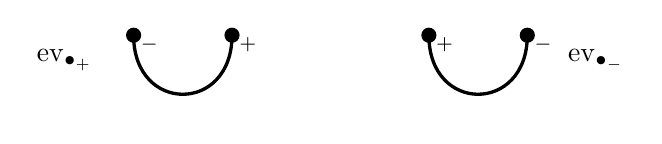
\begin{tikzpicture}[scale=1.25,very thick]
  \filldraw
    (0,0) circle (1.7pt) node[shift={(0.2,-0.12)}] {\scriptsize{$-$}}
    (1,0) circle (1.7pt) node[shift={(0.2,-0.12)}] {\scriptsize{$+$}};
  \draw
    (0,0)
    ..
    controls
    +(0,-0.8)
    and
    +(0,-0.8)
    ..
    (1,0);
  \filldraw
    (3,0) circle (1.7pt) node[shift={(0.2,-0.12)}] {\scriptsize{$+$}}
    (4,0) circle (1.7pt) node[shift={(0.2,-0.12)}] {\scriptsize{$-$}};
  \draw
    (3,0)
    ..
    controls
    +(0,-0.8)
    and
    +(0,-0.8)
    ..
    (4,0);
  \draw
    (-0.7,-0.25) node[fill=white] {$\mathrm{ev}_{\bullet_{+}}$}
    (4.7,-0.25) node[fill=white] {$\mathrm{ev}_{\bullet_{-}}$};
\end{tikzpicture}
\end{equation*}
As $Z$ is monoidal, $Z([M])$ can be identified with the evaluations for $V$ and $V^{\prime}$ respectively, i.e. we obtain
\begin{align*}
  \mathrm{ev}_{V}
  \colon
  V^{\prime}
  \otimes
  V
  \to
  K
  ,\qquad
  v^{\prime}
  \otimes
  v
  &\mapsto
  v^{\prime}(v)
\end{align*}
or
\begin{align*}
  \mathrm{ev}_{V^{\prime}}
  \colon
  V
  \otimes
  V^{\prime}
  \to
  K
  ,\qquad
  v
  \otimes
  v^{\prime}
  &\mapsto
  v^{\prime}(v)
\end{align*}
for $Z([M])$.
\end{enumerate}
Therefore, in any case the morphisms represented by the closed interval $[0,1]$ are determined by the duality properties of $V$. In the case of the circle $S^{1}$ which has empty in- and out-boundary the TQFT $Z$ must determine an element of $K$. But we already know that this must be the dimension $\dim(V)$ of the vector space $V$ since the circle can be understood as a representation of
\begin{align*}
  \mathrm{ev}_{\bullet_{+}}
  \circ
  \mathsf{B}
  \left(
    \bullet_{+}
    ,
    \bullet_{-}
  \right)
  \circ
  \mathrm{coev}_{\bullet_{+}}
\end{align*}
(cf. corollary \ref{cor:dimS1} in chapter \ref{CHAP:ALTCHARPROPS}), where $\mathrm{B}$ is the symmetric braiding of $\mathbf{Cob}_{1}$. Hence we see that $Z$ is entirely determined (at least up to isomorphism) by specifying the finite-dimensional vector space $Z(\bullet_{+}) = V$. And indeed, one can construct a one-dimensional TQFT from every finite dimensional vector space in the above way, so that we basically have a 1-to-1 correspondence between 1-dimensional TQFTs and finite dimensional vector spaces.
\\
This illustrates that even though a priori there are many data to specify for a TQFT, it may be already determined by only a small part of these data - in the 1-dimensional case, for example, by only one datum. Note however that manifolds which need not be specified explicitly may still carry interesting information - in the 1-dimensional case, for example, one obtains the dimension of the vector space which determines the TQFT by considering the circle $S^{1}$ (which, as seen in corollary \ref{cor:dimS1} in chapter \ref{CHAP:ALTCHARPROPS}, can be generalized to higher dimensions).
\\
Now the 1-dimensional TQFTs are the objects of the category
\begin{align*}
  \mathbf{TQFT}_{1}
  &=
  \mathrm{func}^{\otimes,\mathrm{sym}}
  \left(
    \mathbf{Cob}_{1}
    ,
    \mathbf{Vec}_{K}
  \right)
\end{align*}
the morphisms being the monoidal natural transformations, and in fact this category is a groupoid. To cast this example in a nice categorical language we would like to have some algebraic structure that forms a groupoid and captures the structure of finite-dimensional vector spaces in such a way that this groupoid is equivalent to the groupoid of 1-dimensional TQFTs. The natural choice seems to be the category $\mathbf{Finvec}_{K}$ of finite-dimensional vector spaces and linear maps as morphisms. But unfortunately this is not a groupoid since linear maps need not be invertible. Yet, there is an underlying groupoid of this category obtained by discarding all non-invertible linear maps and this is indeed equivalent to $\mathbf{TQFT}_{1}$. But there also is another category in which the inherent duality structure of objects is made a bit more explicit: the category $\mathbf{DP}_{K}$ of dual pairs as described, for example, in \cite{0a816f4c} with the following data
\begin{enumerate}
\item[$\bullet$]
objects are tuples $(V_{1},V_{2},b,d)$ consisting of vector spaces $V_{1},V_{2}$ and two linear maps
\begin{align*}
  b
  \colon
  K
  &\to
  V_{1}
  \otimes
  V_{2}
  ,\qquad
  d
  \colon
  V_{2}
  \otimes
  V_{1}
  \to
  K
\end{align*}
usually called {\glqq}birth{\grqq} and {\glqq}death{\grqq}, which satisfy the conditions (LD1) and (LD2) for dual objects (as vector spaces)

\item[$\bullet$]
morphisms from objects $(V_{1},V_{2},b,d)$ to $(\hat{V}_{1},\hat{V}_{2},\hat{b},\hat{d})$ are pairs $(f_{1},f_{2})$ of linear maps $f_{1} \colon V_{1} \to \hat{V}_{1}$ and $f_{2} \colon V_{2} \to \hat{V}_{2}$ that are subject to the following constraints
\begin{align*}
  (f_{1} \otimes f_{2})
  \circ
  b
  &=
  \hat{b}
  ,\qquad
  d
  =
  \hat{d}
  \circ
  (f_{2} \otimes f_{1})
\end{align*}
\end{enumerate}
Note that the duality conditions for objects enforce the vector spaces in an object of $\mathbf{DP}_{K}$ to be of the same finite dimension. Note further that the conditions for morphisms encode their compatibility with the duality structure and in fact this ensures that they are invertible (this can be seen in a similar way as in the proof of theorem \ref{thm:mntiso} in chapter \ref{CHAP:ALTCHARPROPS}) so that $\mathbf{DP}_{K}$ is a groupoid. Now one can show that the assignment
\begin{align*}
  Z
  &\mapsto
  \left(
    Z(\bullet_{+})
    ,
    Z(\bullet_{-})
    ,
    \mathrm{coev}_{Z(\bullet_{+})}
    ,
    \mathrm{ev}_{Z(\bullet_{+})}
  \right)
\end{align*}
induces a functor that is an equivalence between $\mathbf{TQFT}_{1}$ and $\mathbf{DP}_{K}$.
\\
One can also phrase this example in yet another way, namely by a generators-and-relations approach in terms of free(ly) (generated) symmetric monoidal categories. Given a set $G_{0}$ of objects, a set $G_{1}$ of morphisms and a set $G_{2}$ of relations the morphisms in $G_{1}$ are subject to, one can construct a symmetric monoidal category $\mathbf{F}(G_{0},G_{1},G_{2})$ satisfying a universal property which can basically, but a bit unprecisely, be stated as follows:
\begin{quotation}
For $\mathbf{C}$ a symmetric monoidal category, a symmetric monoidal functor from $\mathbf{F}(G_{0},G_{1},G_{2})$ to $\mathbf{C}$ is determined uniquely up to natural monoidal isomorphism by choosing an object in $\mathrm{ob}_{\mathbf{C}}$ for each element in $G_{0}$ and a morphism in $\mathrm{Mor}_{\mathbf{C}}$ with correct source and target for every element in $G_{1}$ in such a way that the relations in $G_{2}$ are satisfied.
\end{quotation}
This category $\mathbf{F}(G_{0},G_{1},G_{2})$ is consequently unique up to natural monoidal isomorphism and is called the \textit{symmetric monoidal category freely generated by $G_{0},G_{1},G_{2}$}. A nice overview for this construction is given in \cite{0a816f4c}. One can show that $\mathbf{Cob}_{1}$ is freely generated by objects
\begin{align*}
  G_{0}
  &=
  \lbrace
    \bullet_{+}
    ,
    \bullet_{-}
  \rbrace
\end{align*}
morphisms
\begin{align*}
  G_{1}
  &=
  \lbrace
    \mathrm{coev}_{\bullet_{+}}
    ,
    \mathrm{ev}_{\bullet_{+}}
  \rbrace
\end{align*}
and relations $G_{2}$ the duality constraints\footnote{the careful reader may have noticed that apart from $\bullet_{+}$ all other data are determined by duality; for this reason one also says that $\mathbf{Cob}_{1}$ is the \textit{free symmetric monoidal category with duals generated by one object}}. Going through the construction, as is done in \cite{0a816f4c}, one hence obtains precisely the equivalence between $\mathbf{TQFT}_{1}$ and $\mathbf{DP}_{K}$.



\section{2-Dimensional TQFTs}
\label{sec:2dimtqft}
%\nocite{bf5195ee}
%\nocite{0a816f4c}
%\nocite{222239ff}
%\nocite{d37d0fca}
%\nocite{dfcdc48c}
%\nocite{ee9a1449}
%\nocite{00000001}
%%%
Now one may wonder whether there is an equally easy classification for TQFTs in higher dimensions, in particular whether one datum suffices to determine a TQFT. We thus continue with a short overview of the classification of 2-dimensional ordinary TQFTs, i.e. symmetric monoidal functors
\begin{align*}
  Z
  \colon
  \mathbf{Cob}_{2}
  &\to
  \mathbf{Vec}_{K}
\end{align*}
We explore a generators-and-relations approach. The only connected closed smooth 1-manifold is, up to diffeomorphism, the circle $S^{1}$ and as there is an orientation-reversing diffeomorphism on $S^{1}$ the orientation does not really matter. Thus all objects of $\mathbf{Cob}_{2}$ are orientation-preserving diffeomorphic to a finite disjoint union of circles, so as a set of generators for $\mathbf{Cob}_{2}$ on the level of objects we can take $G_{1} = \lbrace S^{1} \rbrace$. On the level of morphisms one can show, e.g. using Morse theory (see appendix), that the following cobordisms suffice to build up all equivalence classes of smooth cobordisms by composition and disjoint union, which means that any surface can basically be chopped into these pieces
\\
\begin{figure}[h!]
\centering
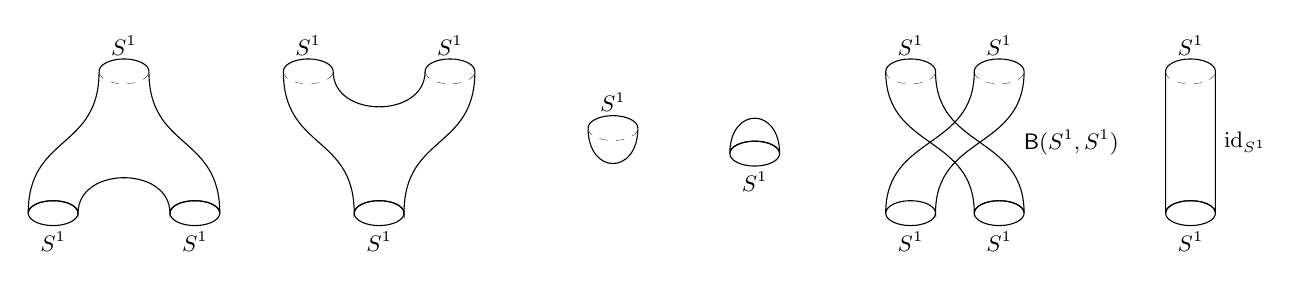
\begin{tikzpicture}[tqft/cobordism/.style={draw},scale=0.9,every node/.style={transform shape}]
  %pants
  \pic[tqft/pair of pants,name=pp,every incoming lower boundary component/.style={draw,ultra thin,dashed},every outgoing boundary component/.style={draw}];
  \node[at=(pp-incoming boundary 1),above=3pt,font=\small]{$S^{1}$};
  \node[at=(pp-outgoing boundary 1),below=4pt,font=\small]{$S^{1}$};
  \node[at=(pp-outgoing boundary 2),below=4pt,font=\small]{$S^{1}$};

  %reverse pants
  \pic[tqft/reverse pair of pants,name=rp,anchor={(-0.3,0)},at=(pp-incoming boundary 1),every incoming lower boundary component/.style={draw,ultra thin,dashed},every outgoing boundary component/.style={draw}];
  \node[at=(rp-incoming boundary 1),above=3pt,font=\small]{$S^{1}$};
  \node[at=(rp-incoming boundary 2),above=3pt,font=\small]{$S^{1}$};
  \node[at=(rp-outgoing boundary 1),below=4pt,font=\small]{$S^{1}$};

  %cup
  \pic[tqft/cup,name=cup,anchor={(-0.15,-0.4)},at=(rp-incoming boundary 2),every incoming lower boundary component/.style={draw,ultra thin,dashed},every outgoing boundary component/.style={draw}];
  \node[at=(cup-incoming boundary 1),above=3pt,font=\small]{$S^{1}$};

  %cap
  \pic[tqft/cap,name=cap,anchor={(-0.0,0.82)},at=(cup-incoming boundary 1),every incoming lower boundary component/.style={draw,ultra thin,dashed},every outgoing boundary component/.style={draw}];
  \node[at=(cap-outgoing boundary 1),below=4pt,font=\small]{$S^{1}$};

  %braiding
  %left-right
  \pic[tqft/cylinder to next,name=l,boundary separation=2.5cm,anchor={(-2.4,0)},at=(rp-incoming boundary 1),every incoming lower boundary component/.style={draw,ultra thin,dashed},every outgoing boundary component/.style={draw}];
  \node[at=(l-incoming boundary 1),above=3pt,font=\small]{$S^{1}$};
  \node[at=(l-outgoing boundary 1),below=4pt,font=\small]{$S^{1}$};
  %right-left
  \pic[tqft/cylinder to prior,name=r,boundary separation=2.5cm,anchor={(0.5,0)},at=(l-incoming boundary 1),every incoming lower boundary component/.style={draw,ultra thin,dashed},every outgoing lower boundary component/.style={draw}];
  \node[at=(r-incoming boundary 1),above=3pt,font=\small]{$S^{1}$};
  \node[at=(r-outgoing boundary 1),below=4pt,font=\small]{$S^{1}$};
  \node[at=(r-between first incoming and first outgoing),right=1.2cm,font=\small]{$\mathsf{B}(S^{1},S^{1})$};

  %cylinder
  \pic[tqft/cylinder,name=c,anchor={(-0.35,0)},at=(r-incoming boundary 1),every incoming lower boundary component/.style={draw,ultra thin,dashed},every outgoing boundary component/.style={draw}];
  \node[at=(c-incoming boundary 1),above=3pt,font=\small]{$S^{1}$};
  \node[at=(c-outgoing boundary 1),below=4pt,font=\small]{$S^{1}$};
  \node[at=(c-between first incoming and first outgoing),right=0.7cm,font=\small]{$\mathrm{id}_{S^{1}}$};
\end{tikzpicture}
\caption{Illustration of generating morphisms for $\mathbf{Cob}_{2}$}
\label{fig:generators}
\end{figure}
\\
All boundary components are circles $S^{1}$, which is why we usually omit the label from now on. The first and second cobordism are often called pair of pants and reverse pair of pants, respectively. We denote the corresponding morphisms by $PP$ and $RP$. We call the third and fourth cobordism cup and cap and denote the corresponding morphisms accordingly by $CUP$ and $CAP$. The identity $\mathrm{id}_{S^{1}}$ and the braiding $\mathsf{B}(S^{1},S^{1})$ are not needed in the set $G_{1}$ of generators as they are automatically included in a freely generated symmetric monoidal category. Thus we take
\begin{align*}
  G_{1}
  &=
  \lbrace
    PP
    ,
    RP
    ,
    CUP
    ,
    CAP
  \rbrace
\end{align*}
for the morphism generators. There are several relations for these generators. We start with the relations involving {\glqq}sewing in a disc{\grqq} which means that we close one of the out-boundaries of the pair of pants, or one of the in-boundaries of the reverse pair of pants, with a disc. To do this in a smooth way we use the cup and the cap and obtain the follwing (illustrations of) relations
\\
\begin{figure}[h!]
\centering
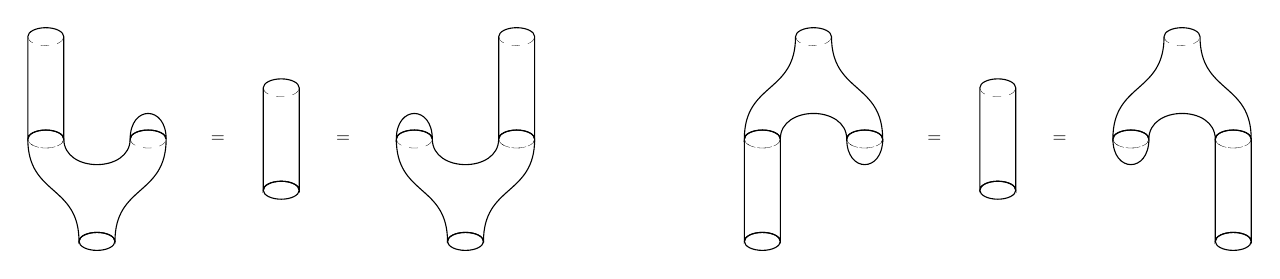
\begin{tikzpicture}[tqft/cobordism/.style={draw},scale=0.65,every node/.style={transform shape}]
  %left
  %reverse pants sewed right
  \pic[tqft/reverse pair of pants,name=rp,every incoming lower boundary component/.style={draw,ultra thin,dashed},every outgoing boundary component/.style={draw}];
  \pic[tqft/cylinder,name=rc,anchor=outgoing boundary 1,at=(rp-incoming boundary 1),every incoming lower boundary component/.style={draw,ultra thin,dashed},every outgoing boundary component/.style={draw,ultra thin,dashed}];
  \pic[tqft/cap,name=cap,anchor=outgoing boundary 1,at=(rp-incoming boundary 2),every incoming lower boundary component/.style={draw,ultra thin,dashed}];
  \node[at=(rp-incoming boundary 2),right=1.1cm]{$=$};
  %cylinder
  \pic[tqft/cylinder,name=rid,anchor={(-0.3,0.5)},at=(rp-incoming boundary 2),every incoming lower boundary component/.style={draw,ultra thin,dashed},every outgoing boundary component/.style={draw}];
  \node[at=(rid-between first incoming and first outgoing),right=1.3cm]{$=$};
  %reverse pants sewed left
  \pic[tqft/reverse pair of pants,name=rp2,anchor={(-1.6,0)},at=(rp-incoming boundary 2),every incoming lower boundary component/.style={draw,ultra thin,dashed},every outgoing boundary component/.style={draw}];
  \pic[tqft/cap,name=cap2,anchor=outgoing boundary 1,at=(rp2-incoming boundary 1),every incoming lower boundary component/.style={draw,ultra thin,dashed}];
  \pic[tqft/cylinder,name=rc2,anchor=outgoing boundary 1,at=(rp2-incoming boundary 2),every incoming lower boundary component/.style={draw,ultra thin,dashed},every outgoing boundary component/.style={draw,ultra thin,dashed}];
  
  %right
  %pants sewed right
  \pic[tqft/pair of pants,name=pp,anchor={(-6.5,0)},at=(rc-incoming boundary 1),every incoming lower boundary component/.style={draw,ultra thin,dashed},every outgoing boundary component/.style={draw,ultra thin,dashed}];
  \pic[tqft/cylinder,name=c,at=(pp-outgoing boundary 1),every incoming lower boundary component/.style={draw,ultra thin,dashed},every outgoing boundary component/.style={draw}];
  \pic[tqft/cup,name=cup,at=(pp-outgoing boundary 2),every incoming lower boundary component/.style={draw,ultra thin,dashed}];
  \node[at=(pp-outgoing boundary 2),right=1.1cm]{$=$};
  %cylinder
  \pic[tqft/cylinder,name=id,anchor={(-0.3,0.5)},at=(pp-outgoing boundary 2),every incoming lower boundary component/.style={draw,ultra thin,dashed},every outgoing boundary component/.style={draw}];
  \node[at=(id-between first incoming and first outgoing),right=1.3cm]{$=$};
  %pants sewed left
  \pic[tqft/pair of pants,name=pp2,anchor={(-2.6,0)},at=(pp-incoming boundary 1),every incoming lower boundary component/.style={draw,ultra thin,dashed},every outgoing boundary component/.style={draw,ultra thin,dashed}];
  \pic[tqft/cup,name=cup2,at=(pp2-outgoing boundary 1),every incoming lower boundary component/.style={draw,ultra thin,dashed}];
  \pic[tqft/cylinder,name=c2,at=(pp2-outgoing boundary 2),every incoming lower boundary component/.style={draw,ultra thin,dashed},every outgoing boundary component/.style={draw}];
\end{tikzpicture}
\caption{Illustration of sewing in discs}
\label{fig:sewing}
\end{figure}
\\
The cylinders representing the identity are only used to give a correct composition in the category.
\\
Next, we have the following relations we call associativity and coassociativity
\\
\begin{figure}[h!]
\centering
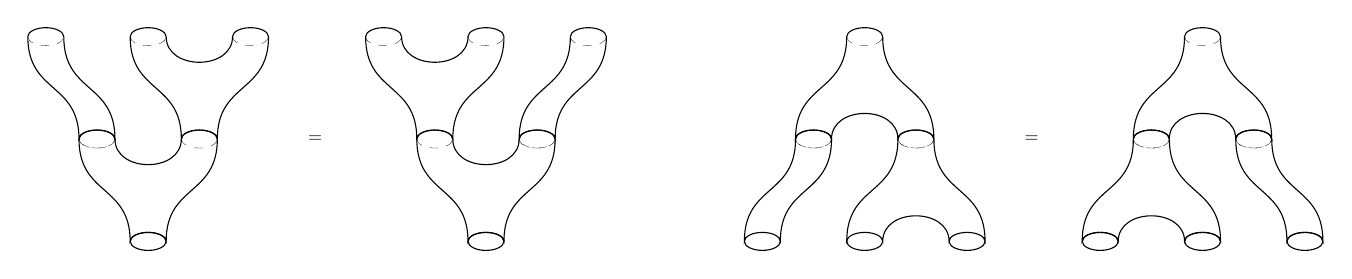
\begin{tikzpicture}[tqft/cobordism/.style={draw},scale=0.65,every node/.style={transform shape}]
  %left
  %right associative
  \pic[tqft/reverse pair of pants,name=rp,every incoming lower boundary component/.style={draw,ultra thin,dashed},every outgoing boundary component/.style={draw}];
  \pic[tqft/cylinder to next,name=rcl,anchor=outgoing boundary 1,at=(rp-incoming boundary 1),every incoming lower boundary component/.style={draw,ultra thin,dashed},every outgoing boundary component/.style={draw,ultra thin,dashed}];
  \pic[tqft/reverse pair of pants,name=rpr,anchor=outgoing boundary 1,at=(rp-incoming boundary 2),every incoming lower boundary component/.style={draw,ultra thin,dashed}];
  \node[at=(rp-incoming boundary 2),right=2cm]{$=$};
  %left associative
  \pic[tqft/reverse pair of pants,name=rp2,anchor={(-1.3,0)},at=(rp-incoming boundary 2),every incoming lower boundary component/.style={draw,ultra thin,dashed},every outgoing boundary component/.style={draw}];
  \pic[tqft/reverse pair of pants,name=rpl,anchor=outgoing boundary 1,at=(rp2-incoming boundary 1),every incoming lower boundary component/.style={draw,ultra thin,dashed}];
  \pic[tqft/cylinder to prior,name=rcr,anchor=outgoing boundary 1,at=(rp2-incoming boundary 2),every incoming lower boundary component/.style={draw,ultra thin,dashed},every outgoing boundary component/.style={draw,ultra thin,dashed}];

  %right
  %right coassociative
  \pic[tqft/pair of pants,name=pp,anchor={(-7,0)},at=(rcl-incoming boundary 1),every incoming lower boundary component/.style={draw,ultra thin,dashed},every outgoing boundary component/.style={draw,ultra thin,dashed}];
  \pic[tqft/cylinder to prior,name=cl,at=(pp-outgoing boundary 1),every incoming lower boundary component/.style={draw,ultra thin,dashed},every outgoing lower boundary component/.style={draw}];
  \pic[tqft/pair of pants,name=ppr,at=(pp-outgoing boundary 2),every incoming lower boundary component/.style={draw,ultra thin,dashed},every outgoing lower boundary component/.style={draw}];
  \node[at=(pp-outgoing boundary 2),right=2cm]{$=$};
  %left coassociative
  \pic[tqft/pair of pants,name=pp2,anchor={(-2.3,0)},at=(pp-incoming boundary 1),every incoming lower boundary component/.style={draw,ultra thin,dashed},every outgoing boundary component/.style={draw,ultra thin,dashed}];
  \pic[tqft/pair of pants,name=ppl,at=(pp2-outgoing boundary 1),every incoming lower boundary component/.style={draw,ultra thin,dashed},every outgoing boundary component/.style={draw}];
  \pic[tqft/cylinder to next,name=cr,at=(pp2-outgoing boundary 2),every incoming lower boundary component/.style={draw,ultra thin,dashed},every outgoing boundary component/.style={draw}];
\end{tikzpicture}
\caption{Illustration of associativity and coassociativity}
\label{fig:assoc}
\end{figure}
\\
Furthermore, the following relations are called commutativity and cocommutativity
\\
\begin{figure}[h!]
\centering
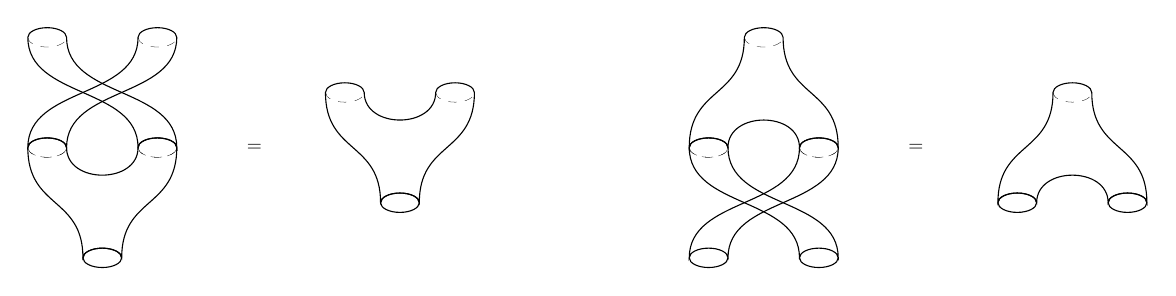
\begin{tikzpicture}[tqft/cobordism/.style={draw},scale=0.7,every node/.style={transform shape}]
  %left
  %reverse pants
  \pic[tqft/reverse pair of pants,name=rp,every incoming lower boundary component/.style={draw,ultra thin,dashed},every outgoing boundary component/.style={draw}];
  %braiding
  \pic[tqft/cylinder to prior,name=rcl,boundary separation=4cm,anchor=outgoing boundary 1,at=(rp-incoming boundary 1),every incoming lower boundary component/.style={draw,ultra thin,dashed},every outgoing boundary component/.style={draw,ultra thin,dashed}];
  \pic[tqft/cylinder to next,name=rcr,boundary separation=4cm,anchor=outgoing boundary 1,at=(rp-incoming boundary 2),every incoming lower boundary component/.style={draw,ultra thin,dashed},every outgoing boundary component/.style={draw,ultra thin,dashed}];
  \node[at=(rp-incoming boundary 2),right=1.5cm]{$=$};
  %reverse pants
  \pic[tqft/reverse pair of pants,name=rp2,anchor={(-0.95,0.5)},at=(rp-incoming boundary 2),every incoming lower boundary component/.style={draw,ultra thin,dashed},every outgoing boundary component/.style={draw}];
  
  %right
  %pants
  \pic[tqft/pair of pants,name=pp,anchor={(-5.5,0)},at=(rcr-incoming boundary 1),every incoming lower boundary component/.style={draw,ultra thin,dashed},every outgoing boundary component/.style={draw,ultra thin,dashed}];
  %braiding
  \pic[tqft/cylinder to next,name=cl,boundary separation=4cm,at=(pp-outgoing boundary 1),every incoming lower boundary component/.style={draw,ultra thin,dashed},every outgoing lower boundary component/.style={draw}];
  \pic[tqft/cylinder to prior,name=cr,boundary separation=4cm,at=(pp-outgoing boundary 2),every incoming lower boundary component/.style={draw,ultra thin,dashed},every outgoing lower boundary component/.style={draw}];
  \node[at=(pp-outgoing boundary 2),right=1.5cm]{$=$};
  %pants
  \pic[tqft/pair of pants,name=pp2,anchor={(-1.8,-0.5)},at=(pp-incoming boundary 1),every incoming lower boundary component/.style={draw,ultra thin,dashed},every outgoing boundary component/.style={draw}];
\end{tikzpicture}
\caption{Illustration of commutativity and cocommutativity}
\label{fig:comm}
\end{figure}
\\
Finally, we have the so-called Frobenius relation
\\
\begin{figure}[h!]
\centering
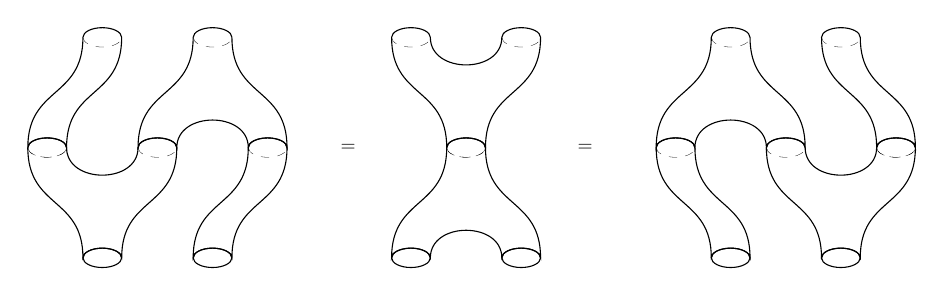
\begin{tikzpicture}[tqft/cobordism/.style={draw},scale=0.7,every node/.style={transform shape}]
  %left
  \pic[tqft/reverse pair of pants,name=rp,every incoming lower boundary component/.style={draw,ultra thin,dashed},every outgoing boundary component/.style={draw}];
  \pic[tqft/pair of pants,name=rpp,anchor=outgoing boundary 1,at=(rp-incoming boundary 2),every incoming lower boundary component/.style={draw,ultra thin,dashed}];
  \pic[tqft/cylinder to prior,name=lc,anchor=outgoing boundary 1,at=(rp-incoming boundary 1),every incoming lower boundary component/.style={draw,ultra thin,dashed},every outgoing boundary component/.style={draw,ultra thin,dashed}];
  \pic[tqft/cylinder to prior,name=rc,at=(rpp-outgoing boundary 2),every incoming lower boundary component/.style={draw,ultra thin,dashed},every outgoing boundary component/.style={draw}];
  \node[at=(rp-incoming boundary 2),right=3.2cm]{$=$};
  
  %middle
  \pic[tqft/pair of pants,name=pp,anchor={(-1.8,0)},at=(rp-incoming boundary 2),every incoming lower boundary component/.style={draw,ultra thin,dashed},every outgoing boundary component/.style={draw}];
  \pic[tqft/reverse pair of pants,name=rp3,anchor=outgoing boundary 1,at=(pp-incoming boundary 1),every incoming lower boundary component/.style={draw,ultra thin,dashed},every outgoing boundary component/.style={draw,ultra thin,dashed}];
  \node[at=(pp-incoming boundary),right=1.9cm]{$=$};
  
  %right
  \pic[tqft/reverse pair of pants,name=rp2,anchor={(-4.7,0)},at=(rp-incoming boundary 2),every incoming lower boundary component/.style={draw,ultra thin,dashed},every outgoing boundary component/.style={draw}];
  \pic[tqft/pair of pants,name=lpp,anchor=outgoing boundary 2,at=(rp2-incoming boundary 1),every incoming lower boundary component/.style={draw,ultra thin,dashed}];
  \pic[tqft/cylinder to next,name=rc2,anchor=outgoing boundary 1,at=(rp2-incoming boundary 2),every incoming lower boundary component/.style={draw,ultra thin,dashed},every outgoing boundary component/.style={draw,ultra thin,dashed}];
  \pic[tqft/cylinder to next,name=lc2,at=(lpp-outgoing boundary 1),every incoming lower boundary component/.style={draw,ultra thin,dashed},every outgoing boundary component/.style={draw}];
\end{tikzpicture}
\caption{Illustration of the Frobenius relation}
\label{fig:frobenius}
\end{figure}
\\
Now the set $G_{2}$ of relations consists of all pairs of morphisms given by one of the above equalities. With the help of Morse theory one can show that this set of relations is sufficient, so that $\mathbf{Cob}_{2}$ is the symmetric monoidal category freely generated by $G_{0},G_{1},G_{2}$. In fact, some of these relations are superfluous and can be omitted. The associativity and coassociativity relations, for example, are both not really needed but also some of the other relations are not necessary. The choice of generators and relations is not unique and there even is no unique minimal choice. The relations here are chosen so because they nicely identify the algebraic structure that corresponds to 2-dimensional TQFTs which we are to explore now briefly.
\\
For a 2-dimensional TQFT $Z \in \mathrm{ob}_{\mathbf{TQFT}_{2}}$ we have a finite-dimensional vector space $V := Z(S^{1})$ associated to the generating object $S^{1}$. This is all we need on the level of objects. On the level of morphisms we start with the reverse pair of pants $RP \in G_{1}$ which has two circles as in-boundary and one circle as out-boundary. Hence, corresponding to $Z(RP)$ we have a linear map
\begin{align*}
  \mu
  \colon
  V
  \otimes
  V
  &\to
  V
\end{align*}
This can be conceived as a bilinear multiplication on $V$, i.e. it makes $V$ into an algebra. The associativity relation in $G_{2}$ shows that $\mu$ is associative. For the cap $CAP \in G_{1}$ which has no in-boundary and a circle as out-boundary we have a linear map corresponding to $Z(CAP)$ of the form
\begin{align*}
  e
  \colon
  K
  &\to
  V
\end{align*}
One of the relations we called sewing in a disc shows that this map is a unit for the multiplication in the sense that
\begin{align*}
  \mu
  \left(
    v
    ,
    e(1)
  \right)
  &=
  v
  =
  \mu
  \left(
    e(1)
    ,
    v
  \right)
\end{align*}
for $v \in V$. So we see that $V$ has the structure of a unital associative algebra. Furthermore, the commutativity relation in $G_{2}$ implies that the multiplication is commutative. In much the same way there is a cocommutative and coassociative comultiplication
\begin{align*}
  \Delta
  \colon
  V
  &\to
  V
  \otimes
  V
\end{align*}
corresponding to $Z(PP)$ and a counit
\begin{align*}
  \varepsilon
  \colon
  V
  &\to
  K
\end{align*}
corresponding to $Z(CUP)$. Finally, the Frobenius relation from $G_{2}$ gives a relation between the multiplication and the comultiplication, again called Frobenius relation, stating that the following diagram commutes
\begin{equation*}
\begin{tikzcd}[row sep=2.7em,column sep=4.2em]
  V \otimes (V \otimes V)
  \ar{dd}[swap]{\mathsf{A}^{-1}(V,V,V)}
  &
  V \otimes V
  \ar{r}{\Delta \otimes \mathrm{id}_{V}}
  \ar{d}{\mu}
  \ar{l}[swap]{\mathrm{id}_{V} \otimes \Delta}
  &
  (V \otimes V) \otimes V
  \ar{dd}{\mathsf{A}(V,V,V)}
  \\
  &
  V
  \ar{d}{\Delta}
  &
  \\
  (V \otimes V) \otimes V
  \ar{r}{\mu \otimes \mathrm{id}_{V}}
  &
  V \otimes V
  &
  V \otimes (V \otimes V)
  \ar{l}[swap]{\mathrm{id}_{V} \otimes \mu}
\end{tikzcd}
\end{equation*}
where $\mathsf{A}$ is the associator in $\mathbf{Vec}_{K}$. Altogether we find that $V$ is a so called commutative Frobenius algebra. For a \textbf{Frobenius algebra} it is actually enough to demand an algebra structure and a coalgebra structure on a vector space that satisfy the Frobenius relation. This automatically ensures associativity and coassociativity. It also already implies that $V$ is finite-dimensional. Moreover, it is enough to demand either commutativity or cocommutativity as they mutually imply each other. There are other equivalent definitions for a Frobenius algebra which do not explicitly mention the coalgebra structure. The reason we chose to give this symmetric definition is that one is immediately led to the right notion of a morphism between Frobenius algebras as being an algebra morphism and a coalgebra morphism at the same time. This means that given two Frobenius algebras
\begin{align*}
  \left(
    V
    ,
    \mu
    ,
    e
    ,
    \Delta
    ,
    \varepsilon
  \right)
  \qquad
  \text{and}
  \qquad
  \left(
    V^{\backprime}
    ,
    \mu^{\backprime}
    ,
    e^{\backprime}
    ,
    \Delta^{\backprime}
    ,
    \varepsilon^{\backprime}
  \right)
\end{align*}
a morphism between them is a linear map $\phi \colon V \to V^{\backprime}$ such that the following diagrams commute
\begin{equation*}
\begin{tikzcd}[row sep=2.7em,column sep=3.6em]
  V \otimes V
  \ar{r}{\mu}
  \ar{d}[swap]{\phi \otimes \phi}
  &
  V
  \ar{d}{\phi}
  \\
  V^{\backprime} \otimes V^{\backprime}
  \ar{r}{\mu^{\backprime}}
  &
  V^{\backprime}
\end{tikzcd}
\qquad
\begin{tikzcd}[row sep=2.7em,column sep=3.6em]
  K
  \ar{r}{e}
  \ar{rd}[swap]{e^{\backprime}}
  &
  V
  \ar{d}{\phi}
  \\
  &
  V^{\backprime}
\end{tikzcd}
\qquad
\qquad
\begin{tikzcd}[row sep=2.7em,column sep=3.6em]
  V \otimes V
  \ar{d}[swap]{\phi \otimes \phi}
  &
  V
  \ar{d}{\phi}
  \ar{l}[swap]{\Delta}
  \\
  V^{\backprime} \otimes V^{\backprime}
  &
  V^{\backprime}
  \ar{l}[swap]{\Delta^{\backprime}}
\end{tikzcd}
\qquad
\begin{tikzcd}[row sep=2.7em,column sep=3.6em]
  K
  &
  V
  \ar{d}{\phi}
  \ar{l}[swap]{\varepsilon}
  \\
  &
  V^{\backprime}
  \ar{ul}{\varepsilon^{\backprime}}
\end{tikzcd}
\end{equation*}
The Frobenius algebras with these morphisms constitute a category $\mathbf{FA}_{K}$ and this category is in fact a groupoid. Furthermore, taking the commutative Frobenius algebras as objects we obtain a full subcategory called $\mathbf{cFA}_{K}$ which of course is again a groupoid. Now, exploring the correspondences above in more detail one can show that they induce an equivalence between $\mathbf{TQFT}_{2}$ and $\mathbf{cFA}_{K}$ so that we indeed have a classification of 2-dimensional TQFTs in terms of an algebraic structure.
\\
There is yet another reason to define a Frobenius algebra as we did above, namely that it can immediately be generalized to the definition of a Frobenius object internal to a monoidal category and similarly a commutative Frobenius object internal to a symmetric monoidal category. For the general setting of monoids internal to (symmetric) monoidal categories the curious reader may have a look at \cite{00000001}. A (commutative) Frobenius algebra is then a (commutative) Frobenius object internal to $\mathbf{Vec}_{K}$. In this more general setting one can form the category of Frobenius objects $\mathbf{cFrob}(\mathbf{C})$ internal to the symmetric monoidal category $\mathbf{C}$. Moreover one can show that $\mathbf{Cob}_{2}$ basically is the free symmetric monoidal category on one commutative Frobenius object and conclude that there is an equivalence of the categories of symmetric monoidal functors $\mathrm{func}^{\otimes,\mathrm{sym}}(\mathbf{Cob}_{2},\mathbf{C})$ and commutative Frobenius objects $\mathbf{cFrob}(\mathbf{C})$. The above classification for 2-dimensional TQFTs is then the special case for the vector space category, $\mathbf{C} = \mathbf{Vec}_{K}$.
\\
For an overview of this classification see e.g. \cite{0a816f4c} and for a fully detailed description the reader is referred to \cite{bf5195ee}. The method of proof there relies on the classification of surfaces (with boundary) so that this method cannot be generalized to higher dimensions. However, there is another proof that uses Cerf theory instead, which basically is a parametrized version of Morse theory. This approach was first suggested by Sawin \cite{222239ff} and full details can be found in the appendix of a work of Moore and Segal \cite{ee9a1449}. This method of proof is generalized to be applicable to extended 2-dimensional TQFTs in \cite{d37d0fca} by Schommer-Pries which treats extended 2-dimensional TQFTs in the language of bicategories (weak 2-categories) in detail. The work includes a systematic approach to the generators-and-relations description of free symmetric monoidal categories in this more general setting. The techniques therein have the potential to be generalized to higher dimensional extended TQFTs. Yet this is not what is done in the work of Lurie\footnote{which in fact pre-dates \cite{d37d0fca}} \cite{dfcdc48c} whose method of proof is quite different and whose formulation, which we want to give here, is cast in the somewhat more elaborate language of $(\infty,n)$-categories. Lurie's less elementary approach to the proof uses an induction and homotopy theoretic techniques, but Morse theory still plays an important role, too. In the next section we will explore what extended TQFTs are and how one arrives there.




\chapter{Extending the Category $\mathbf{Cob}_{n}$}
\label{chap:extcob}
\stepcounter{prpcounter}
%\nocite{904e5e6a}
%%%
So far we have seen classifications for ordinary TQFTs in dimensions $n = 1$ and $n = 2$. In both cases we were able to give a finite set of generating objects and morphisms subject to some relations for the respective cobordism category and only had to deal with this finite amount of data in order to describe TQFTs. In higher dimensions, however, when using this generators-and-relations approach one has to deal with an infinite amount of data. For $n = 3$, for example, one has to take into account all connected, oriented, closed surfaces of genus $g$, for all $g \in \mathbb{N}$, in order to generate the objects so that already the set of generating objects is infinite. This does not mean that it is impossible to give a generators-and-relations description of $\mathbf{Cob}_{n}$ in higher dimensions (see e.g. \cite{904e5e6a}) but it is arguably more cumbersome.
\\
One may also consider TQFTs from a slightly different perspective: we can regard every smooth oriented compact $n$-manifold with boundary $M$ as a cobordism from the empty set to $\partial M$. Then, given an $n$-dimensional TQFT $Z$ we obtain a linear map
\begin{align*}
  Z([M])
  \colon
  Z(\emptyset)
  &\to
  Z(\partial M)
\end{align*}
which can be viewed as a vector in the vector space $Z(\partial M)$ since $Z(\emptyset) \cong K$. Hence $Z([M])$ can be regarded as a diffeomorphism invariant for manifolds. Now as we have seen before in chapter \ref{CHAP:ALTCHARPROPS} we can cut $M$ along embedded closed oriented $(n-1)$-manifolds to calculate this invariant with the help of the evaluation map of the embedded manifold. In particular, suppose we are given a closed oriented $(n-1)$-dimensional submanifold $U \subset M$ which divides $M$ into two pieces $M_{1}$ and $M_{2}$ so that
\begin{align*}
  \partial M_{1}
  \sqcup
  \partial M_{2}
  &\cong
  \partial M
  \sqcup
  \left(
    \overline{U}
    \sqcup
    U
  \right)
\end{align*}
as illustrated exemplarily in figure \ref{fig:cutcob}.
\\
\begin{figure}[h!]
\centering
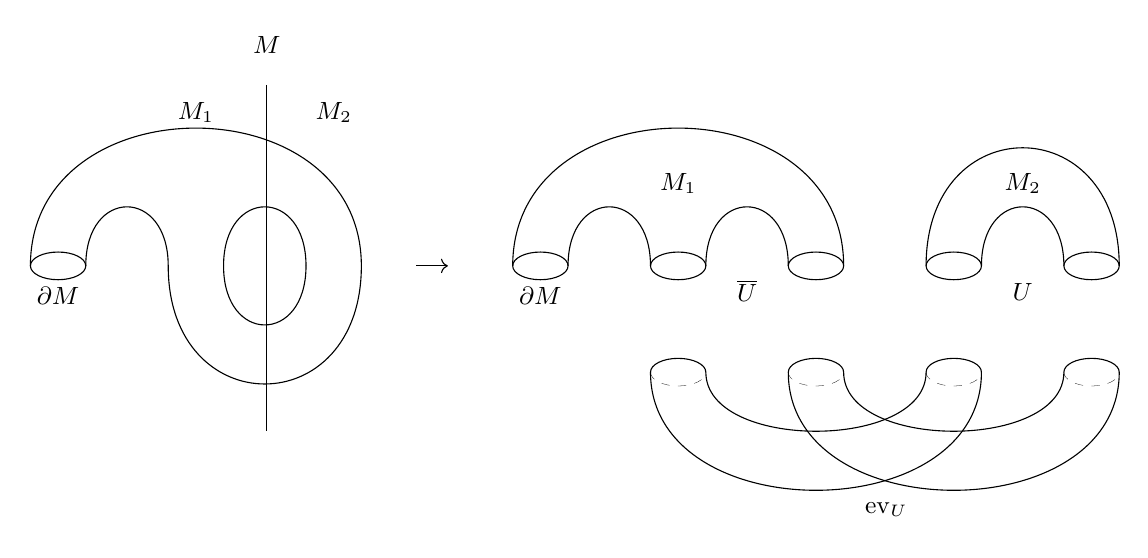
\begin{tikzpicture}[tqft/cobordism edge/.style={draw}]
  %left bottom
  \pic[tqft,name=mb,cobordism height=3cm,boundary separation=1.75cm,incoming boundary components=2,outgoing boundary components=0];

  %left top
  \pic[tqft,name=mt,cobordism height=3cm,boundary separation=1.75cm,incoming boundary components=0,outgoing boundary components=3,anchor=outgoing boundary 2,at=(mb-incoming boundary 1),outgoing boundary component 1/.style={draw}];
  \node[at=(mt-outgoing boundary 2),above=1.7cm,font=\small]{$M_{1}$};
  \node[at=(mt-outgoing boundary 3),above=1.7cm,font=\small]{$M_{2}$};
  \node[at=(mt-outgoing boundary 1),below=4pt,font=\small]{$\partial M$};

  %cutting line
  \draw (0.9,2.3) -- (0.9,-2.1);
  \node[at={(0.9,2.8)}]{\small $M$};

  %arrow
  \draw[->] (2.8,0) -- (3.2,0);

  %right top 1
  \pic[tqft,name=m1,cobordism height=3cm,boundary separation=1.75cm,incoming boundary components=0,outgoing boundary components=3,anchor={(-2.5,1)},at=(mt-outgoing boundary 1),every outgoing boundary component/.style={draw}];
  \node[at=(m1-outgoing boundary 2),above=8mm,font=\small]{$M_{1}$};
  \node[at=(m1-outgoing boundary 1),below=4pt,font=\small]{$\partial M$};
  \node[at=(m1-between outgoing 2 and 3),below=8mm,font=\small]{$\overline{U}$};

  %right top 2
  \pic[tqft,name=m2,cobordism height=3cm,boundary separation=1.75cm,incoming boundary components=0,outgoing boundary components=2,anchor={(-3.5,1)},at=(mt-outgoing boundary 3),every outgoing boundary component/.style={draw}];
  \node[at=(m2-between outgoing 1 and 2),above=0.5mm,font=\small]{$M_{2}$};
  \node[at=(m2-between outgoing 1 and 2),below=8.5mm,font=\small]{$U$};

  %right bottom 1
  \pic[tqft,name=ev1,cobordism height=3cm,boundary separation=3.5cm,incoming boundary components=2,outgoing boundary components=0,anchor={(1,-0.45)},at=(m1-outgoing boundary 2),every incoming upper boundary component/.style={draw},every incoming lower boundary component/.style={draw,ultra thin,dashed}];
  \node[at=(ev1-between incoming 1 and 2),below=10mm,right=5mm,font=\small]{$\mathrm{ev}_{U}$};
  
  %right bottom 2
  \pic[tqft,name=ev2,cobordism height=3cm,boundary separation=3.5cm,incoming boundary components=2,outgoing boundary components=0,anchor={(1,-0.45)},at=(m1-outgoing boundary 3),every incoming upper boundary component/.style={draw},every incoming lower boundary component/.style={draw,ultra thin,dashed}];
\end{tikzpicture}
\caption{Cutting a cobordism in two along a closed submanifold}
\label{fig:cutcob}
\end{figure}
\\
Then we have
\begin{align*}
  Z(\partial M_{1})
  \otimes
  Z(\partial M_{2})
  &\cong
  Z(\partial M)
  \otimes
  \left(
    Z(\overline{U})
    \otimes
    Z(U)
  \right)
\end{align*}
and $Z([M])$ can be obtained from
\begin{align*}
  Z([M_{1}])
  \otimes
  Z([M_{2}])
  \colon
  Z(\emptyset)
  &\to
  Z(\partial M_{1})
  \otimes
  Z(\partial M_{2})
\end{align*}
by applying the pairing $\mathrm{ev}_{Z(U)} \colon Z(\overline{U}) \otimes Z(U) \to K$ induced by $Z(\mathrm{ev}_{U})$ to obtain the map
\begin{equation*}
\begin{tikzcd}[row sep=2.4em,column sep=6em]
  Z(\partial M_{1})
  \otimes
  Z(\partial M_{2})
  \ar{r}{\sim}
  &
  Z(\partial M)
  \otimes
  \left(
    Z(\overline{U})
    \otimes
    Z(U)
  \right)
  \ar{r}{\mathrm{id}_{Z(\partial M)} \otimes \mathrm{ev}_{Z(U)}}
  &
  Z(\partial M)
\end{tikzcd}
\end{equation*}
The question now is whether it is possible to decompose $M$ into {\glqq}simple{\grqq} pieces by cutting along closed submanifolds of codimension $1$, or the other way around, is there a (finite) list of of such {\glqq}simple{\grqq} $n$-manifolds with boundary from which any $n$-manifold can be built up by gluing along  components of the boundaries?
\\
In higher dimensions the pieces one can obtain by cutting along closed submanifolds of codimension 1 are generally not that much simpler than the original manifold and even the submanifolds one cuts along are rather complicated, so the above method becomes less appropriate with growing dimension. We therefore need a more elaborate way of cutting or gluing to obtain simple pieces. The idea is now to not only allow gluing along closed submanifolds but also along submanifolds which themselves have boundary. This means that we have to take care not only of manifolds of dimension $n$ and $n-1$ but also of manifolds of lower dimension. The classical definition of a TQFT does not include this possibility so that we need some elaborate version of this definition.
\\
In section \ref{sec:extdown} we extend the ordinary category $\mathbf{Cob}_{n}$ of cobordisms downwards to obtain an $n$-category which also includes manifolds of all dimensions below $n-1$. In section \ref{sec:extup} we extend the ordinary category $\mathbf{Cob}_{n}$ upwards to an $(\infty,1)$-category which includes also higher homotopical information. Finally, in section \ref{sec:bordn} we combine these two ways of extending $\mathbf{Cob}_{n}$ to obtain the $(\infty,n)$-category $\mathbf{Bord}_{n}$.



\section{Extending Down}
\label{sec:extdown}
%\nocite{29781dd2}
%\nocite{d37d0fca}
%%%
We first extend the category $\mathbf{Cob}_{n}$ to incorporate also manifolds of dimension $n-2$. It seems natural to describe this extension as a $2$-category. We will, however, refrain from giving details (see e.g. \cite{d37d0fca} for them) as this is a little involved. Instead, we will give an informal description to explain the idea. In the following all manifolds are smooth unless stated otherwise.
\\\\
So, let $n \geq 2$ then we can describe the $2$-category ${_{2}}\mathbf{Cob}_{n}$ informally as follows
\begin{enumerate}
\item[(0)]
the objects of ${_{2}}\mathbf{Cob}_{n}$ are closed oriented $(n-2)$-manifolds.

\item[(1)]
for a pair of objects $S_{1},S_{2}$ in ${_{2}}\mathbf{Cob}_{n}$ a $1$-morphism from $S_{1}$ to $S_{2}$ is an oriented $(n-1)$-dimensional $1$-cobordism $M$ with $0$-source $S_{1}$ and $0$-target $S_{2}$ for which we write $M \colon S_{1} \to S_{2}$.

\item[(2)]
for a pair of objects $S_{1},S_{2}$ in ${_{2}}\mathbf{Cob}_{n}$ and a parallel pair of $1$-morphisms $M_{1},M_{2} \colon S_{1} \to S_{2}$ a $2$-morphism from $M_{1}$ to $M_{2}$ is an equivalence class of oriented $n$-dimensional $2$-cobordisms with $1$-source $M_{1}$ and $1$-target $M_{2}$. Note that the $0$-source and $0$-target of these $2$-cobordisms are $S_{1}$ and $S_{2}$.

\item[(c)]
composition of morphisms at both levels is given by gluing cobordisms along the corresponding boundaries
\begin{enumerate}
\item[(1)]
given objects $S_{1},S_{2},S_{3}$ and $1$-morphisms $M_{1}$ from $S_{1}$ to $S_{2}$ and $M_{2}$ from $S_{2}$ to $S_{3}$, their composition $M_{2} \circ M_{1}$ is given by gluing these two $1$-cobordisms along their common boundary $S_{2}$, similar to the $1$-categorical case. Note, however, that since we do not consider diffeomorphism classes at this level, things are a bit more difficult as there are several choices involved and in particular composition is not associative on the nose but only up to isomorphism. Thus ${_{2}}\mathbf{Cob}_{n}$ is a weak $2$-category, not a strict one.

\item[(2)]
for $2$-morphisms there are two kinds of composition
\begin{enumerate}
\item[(v)]
given two objects $S_{1},S_{2}$, three parallel $1$-morphisms $M_{1},M_{2},M_{3}$ from $S_{1}$ to $S_{2}$ and $2$-morphisms $[B_{1}]$ from $M_{1}$ to $M_{2}$ and $[B_{2}]$ from $M_{2}$ to $M_{3}$, their vertical composition $[B_{2}] \circ^{\mathrm{v}} [B_{1}]$ - a $2$-morphism from $M_{1}$ to $M_{3}$ - is basically given by gluing the underlying manifolds with corners $B_{1}$ and $B_{2}$ together along their common boundary $M_{2}$.

\item[(h)]
given three objects $S_{1},S_{2},S_{3}$, two parallel $1$-morphisms $M_{1},M_{2}$ from $S_{1}$ to $S_{2}$, two parallel $1$-morphisms $M_{3},M_{4}$ from $S_{2}$ to $S_{3}$ and $2$-morphisms $[B_{1}]$ from $M_{1}$ to $M_{2}$ and $[B_{2}]$ from $M_{3}$ to $M_{4}$, their horizontal composition $[B_{2}] \circ^{\mathrm{h}} [B_{1}]$ - a $2$-morphism from $M_{3} \circ M_{1}$ to $M_{4} \circ M_{2}$ - is basically given by gluing the underlying $2$-cobordisms $B_{1}$ and $B_{2}$ together along their common boundary $S_{2}$, or more precisely $S_{2} \times [0,1]$.
\end{enumerate}
\end{enumerate}

\item[(i)]
identities for the compositions on both levels are given by taking the product of the source (or equivalently the target, of course) of the identity in question with the unit interval $[0,1]$.

\item[(s)]
there is a symmetric monoidal structure on ${_{2}}\mathbf{Cob}_{n}$ given on all levels by disjoint union.
\end{enumerate}
This extended cobordism $2$-category ${_{2}}\mathbf{Cob}_{n}$ contains the category $\mathbf{Cob}_{n}$ as the looping at $\emptyset$: fix the empty $(n-2)$-manifold $\emptyset$ as source and target object, then the $1$-morphisms with this source and target are actually oriented closed $(n-1)$-manifolds and $2$-morphisms between such $1$-morphisms are actually (equivalence classes of) $n$-dimensional $1$-cobordisms. Hence the category
\begin{align*}
  _{1}\mathbf{mor}_{{_{2}}\mathbf{Cob}_{n}}
  \left(
    \emptyset
    ,
    \emptyset
  \right)
  &=
  \Omega_{\emptyset}
  \left(
    {_{2}}\mathbf{Cob}_{n}
  \right)
\end{align*}
is equivalent to $\mathbf{Cob}_{n}$. Therefore, to define an extended version of TQFTs on ${_{2}}\mathbf{Cob}_{n}$ one might try to find a target $2$-category ${_{2}}\mathbf{Vec}_{K}$ that contains $\mathbf{Vec}_{K}$ in the same sense. There are many different possible such $2$-categories and different choices may be well-suited for different intended uses. One can also argue that any symmetric monoidal $2$-category describing algebraic structures or even more generally any symmetric monoidal $2$-category may serve as a target for an extended TQFT. We adopt the latter approach here. Thus let ${_{2}}\mathbf{C}$ be a symmetric monoidal $2$-category, then an \textbf{$n$-dimensional $2$-extended ${_{2}}\mathbf{C}$-valued (oriented) topological quantum field theory} is a symmetric monoidal functor
\begin{align*}
  Z
  \colon
  {_{2}}\mathbf{Cob}_{n}
  &\to
  {_{2}}\mathbf{C}
\end{align*}
of $2$-categories. We will usually use the abbreviation TQFT and will frequently supress the dimension $n$ and the category ${_{2}}\mathbf{C}$ if they are understood and hence simply speak of a $2$-extended TQFT.
\\
Note that if ${_{2}}\mathbf{C}$ is some appropriate version of ${_{2}}\mathbf{Vec}_{K}$ then such a $2$-extended TQFT induces an ordinary TQFT by restricting to the looping $\Omega_{\emptyset}({_{2}}\mathbf{Cob}_{n})$ of ${_{2}}\mathbf{Cob}_{n}$ at $\emptyset$.
\\
For a closed $n$-manifold $M$ we now have more flexibility to calculate the corresponding invariant given by a TQFT as we can cut it along $(n-1)$-submanifolds with boundary $N$ and we can cut the latter along closed $(n-2)$-submanifolds. However, if the dimension $n$ is large then $N$ may be fairly complicated and cutting along closed manifolds will still not simplify it very much in general. Therefore we also want to allow cutting $N$ along $(n-2)$-submanifolds with boundary, i.e. we push the idea of extending further by adding another layer to the cobordism category. More generally, let $n,k \in \mathbb{N}$ with $k \leq n$, then we can describe the $k$-category ${_{k}}\mathbf{Cob}_{n}$ informally as follows (we will be a bit briefer here than in the description of ${_{2}}\mathbf{Cob}_{n}$)
\begin{enumerate}
\item[(0)]
the objects of ${_{k}}\mathbf{Cob}_{n}$ are closed oriented $(n-k)$-manifolds.

\item[(1)]
for a pair of objects $S_{1},S_{2}$ in ${_{k}}\mathbf{Cob}_{n}$ a $1$-morphism from $S_{1}$ to $S_{2}$ is an oriented $(n-k+1)$-dimensional $1$-cobordism $M$ with $0$-source $S_{1}$ and $0$-target $S_{2}$, written as $M \colon S_{1} \to S_{2}$.

\item[(2)]
for a pair of objects $S_{1},S_{2}$ in ${_{k}}\mathbf{Cob}_{n}$ and a pair of parallel $1$-morphisms $M_{1},M_{2} \colon S_{1} \to S_{2}$ a $2$-morphism from $M_{1}$ to $M_{2}$ is an oriented $(n-k+2)$-dimensional $2$-cobordism with $1$-source $M_{1}$ and $1$-target $M_{2}$.

\item[]
\begin{equation*}
\vdots
\end{equation*}
\item[]

\item[(k)]
a $k$-morphism is an equivalence class of oriented $n$-dimensional $k$-cobordisms.

\item[(c)]
composition of morphisms at all levels is given by gluing cobordisms along the corresponding boundaries.

\item[(s)]
there is a symmetric monoidal structure on ${_{k}}\mathbf{Cob}_{n}$ given on all levels by disjoint union.
\end{enumerate}
This category is of course again not strict. In the case $k = 1$ the category ${_{k}}\mathbf{Cob}_{n}$ is just the ordinary cobordism category $\mathbf{Cob}_{n}$. In the case $k = 0$ the category ${_{k}}\mathbf{Cob}_{n}$ can be viewed as the set of diffeomorphism classes of oriented closed $n$-manifolds.
\\
We can now generalize the $2$-extended case of TQFTs. Let ${_{k}}\mathbf{C}$ be a symmetric monoidal $k$-category, then an \textbf{$n$-dimensional $k$-extended ${_{k}}\mathbf{C}$-valued (oriented) topological quantum field theory} is a symmetric monoidal functor
\begin{align*}
  Z
  \colon
  {_{k}}\mathbf{Cob}_{n}
  &\to
  {_{k}}\mathbf{C}
\end{align*}
of $k$-categories. Again, we will usually use the abbreviation TQFT and will frequently supress the dimension $n$ and the category ${_{k}}\mathbf{C}$ if they are understood and thus simply speak of a $k$-extended TQFT. Moreover, if $k = n$ we will usually omit it as well, and just say extended TQFT.
\\
Such an extended TQFT may generally seem to be more complicated than an ordinary TQFT since it is phrased in terms of higher categories and involves many more data because it can be evaluated on manifolds (with corners) of arbitrary dimension below $n+1$. Yet, since an extended TQFT is a functor of $n$-categories, we have much more flexibility in decomposing manifolds into simpler pieces. A closed $n$-manifold $M$ may look rather complicated globally, but locally it is, of course, very simple since for any point $x \in M$ there is a neighbourhod which is diffeomorphic to (an open subset of) $\mathbb{R}^{n}$. We therefore hope that we can decompose $M$ in only few different and very simple pieces, so that we only have to specify the TQFT on these data. In the case $n = 1$, where an extended $\mathbf{Vec}_{K}$-valued TQFT is nothing but an ordinary TQFT, we saw that one only needs to specify a finite vector space associated to the manifold consisting of a single point.
\\
In general it is not true that an extended oriented TQFT is determined by giving an appropriate object of the target category as value for the manifold consisting of a single point. Here are two reasons why:
\begin{enumerate}
\item
For a closed manifold $M$ there is an open neighbourhood for each point $x \in M$ diffeomorphic to $\mathbb{R}^{n}$ but there is no unique or canonical choice. In a more canonical way one can choose an open neighbourhood $U$ of $x$ and a diffeomorphism $\varphi \colon U \to B$ to an open ball $B$ in the tangent space $T_{x}M$ at $x$. This is still not unique but leads to a contractible space of choices of such $\varphi$ if we require the differential $T_{x}\varphi \colon T_{x}U \to T_{\varphi(x)}B$ of the diffeomorphism $\varphi$ at $x$ - which reduces to an automorphism of $T_{x}M$ when identifying $T_{x}U$ with $T_{x}M$ and the tangent space $T_{\varphi(x)}T_{x}M \cong T_{\varphi(x)}B$ of $T_{x}M$ with $T_{x}M$ itself via the so-called vertical lift - to be the identity on $T_{x}M$. In the case $n = 1$ the orientation of the manifold yields a trivialization of the tangent bundle $TM$ so that we have a canonical way to identify $T_{x}M$ with $\mathbb{R}^{n}$. In higher dimensions, however, an orientation does not automatically imply that $TM$ can be trivialized.

\item
Even for $n = 1$ and ${_{1}}\mathbf{C} = \mathbf{Vec}_{K}$ one cannot choose any object to determine the TQFT. In fact, the vector space chosen must be finite dimensional. Thus we must expect that there is some (more general) finiteness condition to be imposed in the general case, too.
\end{enumerate}
To solve the first problem we use the stronger structure of framings instead of orientations for the manifolds in the cobordism category. A \textbf{framing} of a real $n$-dimensional vector bundle $\zeta$ is a trivialization, i.e. an isomorphism of vector bundles to the product vector bundle $\mathrm{pr}_{1} \colon B \times \mathbb{R}^{n} \to B$. For $k \leq n \in \mathbb{N}$ an \textbf{$n$-framing} of a $k$-dimensional manifold with corners $M$ is a framing of the vector bundle
\begin{align*}
  TM
  \oplus
  \left(
    M
    \times
    \mathbb{R}^{n-k}
  \right)
\end{align*}
sometimes called the \textbf{$n$-stabilized tangent bundle}. The framed version ${_{n}}\mathbf{Cob}_{n}^{\mathrm{fr}}$ of the cobordism $n$-category is now basically defined in the same way as ${_{n}}\mathbf{Cob}_{n}$ except that all manifolds are equipped with $n$-framings - where for $n$-morphisms this $n$-framing is taken up to homotopy - and the framings of all morphisms are compatible with the framings of their source and target just as in the oriented case. For a symmetric monoidal $n$-category ${_{n}}\mathbf{C}$ a \textbf{framed extended ${_{n}}\mathbf{C}$-valued TQFT} is then a symmetric monoidal functor
\begin{align*}
  Z
  \colon
  {_{n}}\mathbf{Cob}_{n}^{\mathrm{fr}}
  &\to
  {_{n}}\mathbf{C}
\end{align*}
of $n$-categories.
\\
For the second problem remember that the finiteness condition in the case $n = 1$ was due to the dualizability of objects in $\mathbf{Cob}_{n}$. We will thus introduce the concept of fully dualizable objects in symmetric monoidal $n$-categories which is a generalization of what it means for objects to be dualizable in ordinary symmetric monoidal categories. This is however postponed until chapter \ref{chap:formcobhyp} as we first carry on extending the cobordism category to the final version we use to state the cobordism hypothesis.



\section{Extending Up}
\label{sec:extup}
%\nocite{dfcdc48c}
%%%
So far we extended the ordinary cobordism category $\mathbf{Cob}_{n}$ downwards by adding levels for lower dimensional manifolds. There is another way of extending $\mathbf{Cob}_{n}$, namely by not using diffeomorphism classes of cobordisms as morphisms but instead using also higher morphisms to keep track of these diffeomorphisms and how they are related to each other. For a pair of parallel $1$-cobordisms
\begin{align*}
  M_{1}
  ,
  M_{2}
  \colon
  S_{1}
  &\to
  S_{2}
\end{align*}
between objects $S_{1},S_{2}$ the set of orientation-preserving diffeomorphisms rel boundary $C_{rb}^{\infty}(M_{1},M_{2})$ usually comes with the so-called topology of uniform convergence of all derivatives, also called Whitney $C^{\infty}$ topology, and endowing all the diffeomorphism sets with this topology makes composition continuous. We can thus define a \textit{topologically enriched category}\footnote{a topologically enriched category is a category enriched over the category of (compactly generated) topological spaces} $\mathbf{D}(S_{1},S_{2})$ with objects $1$-cobordisms from $S_{1}$ to $S_{2}$ and morphisms the corresponding diffeomorphism sets with the above topology. This additional homotopical structure is lost in the classical definition of $\mathbf{Cob}_{n}$ and one might wish to include it in an elaborated version. As a further motivation the interested reader may have a look at \cite{dfcdc48c} for example. There the usual morphism sets $\mathrm{mor}_{\mathbf{Cob}_{n}}(S_{1},S_{2})$ are replaced by the classifying spaces\footnote{remember that the classifying space of a category is the geometric realization of its nerve} of the categories $\mathbf{D}(S_{1},S_{2})$ in order to describe symmetric monoidal functors into the category of chain complexes which yield TQFTs by passing to homology.
\\
The language of higher categories allows us to capture this structure in the light of the homotopy hypothesis which, from a homotopical perspective, allows us to replace a topological space by its fundamental $\infty$-groupoid. This means that instead of using the ordinary categories $\mathbf{D}(S_{1},S_{2})$ as mapping categories we use the corresponding $(\infty,1)$-categories obtained by replacing the morphism spaces of each $\mathbf{D}(S_{1},S_{2})$ by their fundamental $\infty$-groupoids. These $(\infty,1)$-categories are actually $(\infty,0)$-categories since diffeomorphisms - which are the $1$-morphisms here - are invertible. Hence the elaboration ${_{(\infty,1)}}\mathbf{Cob}_{n}$ of $\mathbf{Cob}_{n}$ can informally be described as an $(\infty,1)$-category as follows
\begin{enumerate}
\item[(0)]
the objects of ${_{(\infty,1)}}\mathbf{Cob}_{n}$ are the objects of $\mathbf{Cob}_{n}$, i.e. closed oriented $(n-1)$-manifolds

\item[(1)]
for a pair of objects $S_{1},S_{2}$ in ${_{(\infty,1)}}\mathbf{Cob}_{n}$ a $1$-morphism from $S_{1}$ to $S_{2}$ is an oriented $n$-dimensional $1$-cobordism $M \colon S_{1} \to S_{2}$

\item[(2)]
for a pair of objects $S_{1},S_{2}$ in ${_{(\infty,1)}}\mathbf{Cob}_{n}$ and a pair of parallel $1$-morphisms $M_{1},M_{2} \colon S_{1} \to S_{2}$ a $2$-morphism from $M_{1}$ to $M_{2}$ is an orientation-preserving diffeomorphism rel boundary $f_{12}$ between them, written $f_{12} \colon M_{1} \Rightarrow M_{2}$

\item[(3)]
given a pair of objects $S_{1},S_{2}$ in ${_{(\infty,1)}}\mathbf{Cob}_{n}$, a pair of parallel $1$-morphisms $M_{1},M_{2} \colon S_{1} \to S_{2}$ and a pair of parallel $2$-morphisms $f,g$ from $M_{1}$ to $M_{2}$, then a $3$-morphism from $f$ to $g$ is a smooth homotopy between them

\item[]
\begin{equation*}
\vdots
\end{equation*}
\item[]

\item[(...)]
higher morphisms are higher (smooth) homotopies between the lower ones

\item[]
\begin{equation*}
\vdots
\end{equation*}
\item[]

\item[(c)]
\begin{enumerate}
\item[(1)]
composition of morphisms on level $1$ is given by gluing cobordisms

\item[(2)]
on level $2$ vertical and horizontal composition have to be distinguished
\begin{enumerate}
\item[(v)]
vertical composition is given by the usual composition of functions

\item[(h)]
for the horizontal composition let $M_{12},M_{12}^{\backprime} \colon S_{1} \to S_{2}$ and $M_{23},M_{23}^{\backprime} \colon S_{1} \to S_{2}$ be $1$-morphisms and let $f_{12} \colon M_{12} \Rightarrow M_{12}^{\backprime}$ and $f_{23} \colon M_{23} \Rightarrow M_{23}^{\backprime}$ be $2$-morphisms, then their horizontal composition
\begin{align*}
  f_{23}
  \circ^{\mathrm{h}}
  f_{12}
  \colon
  M_{23}
  \circ
  M_{12}
  &\Rightarrow
  M_{23}^{\backprime}
  \circ
  M_{12}^{\backprime}
\end{align*}
is given by {\glqq}merging{\grqq} $f_{12}$ and $f_{23}$ into one function along their common {\glqq}boundary{\grqq} $S_{2}$ which basically means that
\begin{align*}
  f_{23}
  \circ^{\mathrm{h}}
  f_{12}
  (x)
  &=
  f_{12}(x)
  \in
  M_{12}^{\backprime}
  \qquad
  \text{for }
  x
  \in
  M_{12}
  \\
  f_{23}
  \circ^{\mathrm{h}}
  f_{12}
  (x)
  &=
  f_{23}(x)
  \in
  M_{23}^{\backprime}
  \qquad
  \text{for }
  x
  \in
  M_{23}
\end{align*}
Note that this is well-defined, at least up to homotopy, since $f_{12}$ and $f_{23}$ basically have to coincide on $S_{2}$ as they are diffeomorphisms rel boundary, but strictly speaking one has to take the subtleties of gluing cobordisms into account, of course.
\end{enumerate}

\item[(3)]
on the level of $3$-morphisms we have (smooth) homotopies between diffeomorphisms and there are three ways of composing
\begin{enumerate}
\item[(i)]
given $2$-morphisms $f_{12},f_{12}^{\backprime} \colon M_{1} \Rightarrow M_{2}$ and $f_{23},f_{23}^{\backprime} \colon M_{2} \Rightarrow M_{3}$ and $3$-morphisms
\begin{align*}
\hspace{6em}
  h_{1}
  \colon
  f_{12}
  &\Rrightarrow
  f_{12}^{\backprime}
  \quad
  \text{i.e.}
  \quad
  h_{1}
  \colon
  M_{1}
  \times
  [0,1]
  \to
  M_{2}
  ,\quad
  h_{1}(\cdot,0)
  =
  f_{12}
  ,\quad
  h_{1}(\cdot,1)
  =
  f_{12}^{\backprime}
  \\
  h_{2}
  \colon
  f_{23}
  &\Rrightarrow
  f_{23}^{\backprime}
  \quad
  \text{i.e.}
  \quad
  h_{2}
  \colon
  M_{2}
  \times
  [0,1]
  \to
  M_{3}
  ,\quad
  h_{2}(\cdot,0)
  =
  f_{23}
  ,\quad
  h_{2}(\cdot,1)
  =
  f_{23}^{\backprime}
\end{align*}
then, as vertical composition for $2$-morphisms is just function composition, we obtain a new $3$-morphism between the vertical compositions by
\begin{align*}
  &
  h_{2}
  \circ^{i}
  h_{1}
  \colon
  f_{23}
  \circ^{\mathrm{v}}
  f_{12}
  \Rrightarrow
  f_{23}^{\backprime}
  \circ^{\mathrm{v}}
  f_{12}^{\backprime}
  \\
  &
  h_{2}
  \circ^{i}
  h_{1}
  (x,t)
  :=
  h_{2}(h_{1}(x,t),t)
  ,\quad
  (x,t)
  \in
  M_{1}
  \times
  [0,1]
\end{align*}

\item[(ii)]
given $2$-morphisms $f_{12},f_{12}^{\backprime} \colon M_{12} \Rightarrow M_{12}^{\backprime}$ and $f_{23},f_{23}^{\backprime} \colon M_{23} \Rightarrow M_{23}^{\backprime}$ and $3$-morphisms
\begin{align*}
\hspace{6em}
  h_{1}
  \colon
  f_{12}
  &\Rrightarrow
  f_{12}^{\backprime}
  \quad
  \text{i.e.}
  \quad
  h_{1}
  \colon
  M_{12}
  \times
  [0,1]
  \to
  M_{12}^{\backprime}
  ,\quad
  h_{1}(\cdot,0)
  =
  f_{12}
  ,\quad
  h_{1}(\cdot,1)
  =
  f_{12}^{\backprime}
  \\
  h_{2}
  \colon
  f_{23}
  &\Rrightarrow
  f_{23}^{\backprime}
  \quad
  \text{i.e.}
  \quad
  h_{2}
  \colon
  M_{23}
  \times
  [0,1]
  \to
  M_{23}^{\backprime}
  ,\quad
  h_{2}(\cdot,0)
  =
  f_{23}
  ,\quad
  h_{2}(\cdot,1)
  =
  f_{23}^{\backprime}
\end{align*}
then these $3$-morphisms can be merged into a new one between the horizontal compositions of the $2$-morphisms in much the same way as the $2$-morphisms themselves, so basically we have
\begin{align*}
\hspace{8em}
  h_{2}
  \circ^{ii}
  h_{1}
  \colon
  f_{23}
  \circ^{\mathrm{h}}
  f_{12}
  \Rrightarrow
  f_{23}^{\backprime}
  \circ^{\mathrm{h}}
  f_{12}^{\backprime}
  \quad
  \text{i.e.}
  \quad
  &
  h_{2}
  \circ^{ii}
  h_{1}
  \colon
  \left(
    M_{23}
    \circ
    M_{12}
  \right)
  \times
  [0,1]
  \to
  M_{23}^{\backprime}
  \circ
  M_{12}^{\backprime}
  \\
  &
  h_{2}
  \circ^{ii}
  h_{1}
  (x,\cdot)
  :=
  h_{1}(x,\cdot)
  \qquad
  \text{for }
  x
  \in
  M_{12}
  \\
  &
  h_{2}
  \circ^{ii}
  h_{1}
  (x,\cdot)
  :=
  h_{2}(x,\cdot)
  \qquad
  \text{for }
  x
  \in
  M_{23}
\end{align*}

\item[(iii)]
given two $3$-morphisms $h_{12} \colon f_{1} \Rrightarrow f_{2}$ and $h_{23} \colon f_{2} \Rrightarrow f_{3}$ they can be patched together as usual for homotopies, that is, their composition is
\begin{align*}
  &
  h_{23}
  \circ^{iii}
  h_{12}
  \colon
  f_{1}
  \Rrightarrow
  f_{3}
  \\
  &
  h_{23}
  \circ^{iii}
  h_{12}(\cdot,t)
  :=
  h_{12}(\cdot,2t)
  \qquad
  \text{for }
  t
  \in
  [0,0.5]
  \\
  &
  h_{23}
  \circ^{iii}
  h_{12}(\cdot,t)
  :=
  h_{23}(\cdot,2t-1)
  \qquad
  \text{for }
  t
  \in
  [0.5,1]
\end{align*}
\end{enumerate}

\item[(...)]
higher homotopies can be composed in the same way with the difference that there are successively further directions in which one can compose similar to the $iii$-composition of $3$-morphisms
\end{enumerate}

\item[(s)]
using the disjoint union one can again endow ${_{(\infty,1)}}\mathbf{Cob}_{n}$ with a symmetric monoidal structure
\end{enumerate}



\section{The $(\infty,n)$-Category $\mathbf{Bord}_{n}$}
\label{sec:bordn}
%\nocite{dfcdc48c}
%%%
Now we can combine the two preceding subsections to define our final version of the cobordism category which we call $\mathbf{Bord}_{n}$. We will drop the requirement of orientation as standard in this definition as we will consider various structures on the manifolds for this category later. For $n \in \mathbb{N}$ we can thus describe this $(\infty,n)$-category informally as follows
\begin{enumerate}
\item[(0)]
the objects of $\mathbf{Bord}_{n}$ are compact $0$-manifolds

\item[(1)]
for a pair of objects $S_{1},S_{2}$ in $\mathbf{Bord}_{n}$ a $1$-morphism from $S_{1}$ to $S_{2}$ is a $1$-dimensional $1$-cobordism $M \colon S_{1} \to S_{2}$

\item[(2)]
for a pair of objects $S_{1},S_{2}$ in $\mathbf{Bord}_{n}$ and a pair of parallel $1$-morphisms $M_{1},M_{2} \colon S_{1} \to S_{2}$ a $2$-morphism from $M_{1}$ to $M_{2}$ is a $2$-dimensional $2$-cobordism with $1$-source $M_{1}$ and $1$-target $M_{2}$

\item[]
\begin{equation*}
\vdots
\end{equation*}
\item[]

\item[(n)]
an $n$-morphism is an $n$-dimensional $n$-cobordism between two parallel $(n-1)$-dimensional $(n-1)$-cobordisms

\item[(n+1)]
an $(n+1)$-morphism between two parallel $n$-morphisms is a diffeomorphism rel boundary between them

\item[(n+2)]
an $(n+2)$-morphism is a smooth homotopy between its parallel source and target $(n+1)$-morphism, i.e. between parallel diffeomorphisms rel boundary

\item[]
\begin{equation*}
\vdots
\end{equation*}
\item[]

\item[(...)]
higher morphisms are higher (smooth) homotopies between the lower ones

\item[]
\begin{equation*}
\vdots
\end{equation*}
\item[]

\item[(c)]
composition on the various levels of morphisms is as described for ${_{n}}\mathbf{Cob}_{n}$ and ${_{(\infty,n)}}\mathbf{Cob}_{n}$ in the two preceding subsections

\item[(s)]
using the disjoint union one can again endow $\mathbf{Bord}_{n}$ with a symmetric monoidal structure
\end{enumerate}
This symmetric monoidal $(\infty,n)$-category $\mathbf{Bord}_{n}$ can be endowed with additional, often called tangential structures for the manifolds, e.g. orientations or $n$-framings, by requiring all manifolds to be equipped with such a structure in a compatible way. For orientations and $n$-framings we call the corresponding $(\infty,n)$-categories $\mathbf{Bord}_{n}^{\mathrm{or}}$ and $\mathbf{Bord}_{n}^{\mathrm{fr}}$, respectively. In the next section we also introduce a more general way to endow $\mathbf{Bord}_{n}$ with additional structures.
\\
Now for a symmetric monoidal $(\infty,n)$-category ${_{(\infty,n)}}\mathbf{C}$ an \textbf{$n$-dimensional fully extended ${_{(\infty,n)}}\mathbf{C}$-valued TQFT} is a symmetric monoidal functor
\begin{align*}
  Z
  \colon
  \mathbf{Bord}_{n}
  &\to
  {_{(\infty,n)}}\mathbf{C}
\end{align*}
of $(\infty,n)$-categories. If we replace $\mathbf{Bord}_{n}$ by $\mathbf{Bord}_{n}^{\mathrm{or}}$ or $\mathbf{Bord}_{n}^{\mathrm{fr}}$ we add the adjective \textbf{oriented} or \textbf{framed}. For a precise definition of this version of the cobordism category as a symmetric monoidal $(\infty,n)$-category the reader is referred to \cite{29781dd2} where also the case of additional tangential structures (see section \ref{sec:vyzstruct}) is treated. In \cite{dfcdc48c} there is a description, too, which however lacks some details and also contains an error which is corrected by the slightly modified approach in \cite{29781dd2}. Both works use $n$-fold complete Segal spaces as a model for $(\infty,n)$-categories. A major advantage of this approach is that composition does not need to be defined on the nose but rather up to a contractible space of choices. This makes the subtleties of gluing, like dealing with the smooth structure, disappear. The basic idea for the construction is the following.
\\
\begin{cst}[Sketch]
\label{cst:bordn}
For any finite-dimensional vector space $V$ and multiindex
\begin{align*}
  \underline{k}
  &=
  (k_{1},\ldots,k_{n})
  \in
  \mathbb{N}^{n}
\end{align*}
consider the set
\begin{align*}
  \left(
    \mathrm{PBord}_{n}^{V}
  \right)_{\underline{k}}
\end{align*}
consisting of tuples
\begin{align*}
  \left(
    M
    ,
    \left(
      t_{0}^{1}
      ,
      \ldots
      ,
      t_{k_{1}}^{1}
    \right)
    ,
    \ldots
    ,
    \left(
      t_{0}^{n}
      ,
      \ldots
      ,
      t_{k_{n}}^{n}
    \right)
  \right)
\end{align*}
where $M$ is a submanifold of $V \times \mathbb{R}^{n}$ satisfying some properties, the tuple $(t_{0}^{i},\ldots,t_{k_{i}}^{i})$ consists of $k_{i}+1$ real numbers with $t_{0}^{i} \leq \ldots \leq t_{k_{i}}^{i}$ for $i = 1,\ldots,n$ and the manifold and these tuples satisfy another property. The tuples of real numbers are meant to encode where the manifold can be cut in pieces so that one should think of an element in $(\mathrm{PBord}_{n}^{V})_{\underline{k}}$ as a collection of $k_{1} k_{2} \cdots k_{n}$ cobordisms which are glued together in the $n$ possible directions, i.e. $k_{i}$ cobordisms in direction $i$.
\\
The next step is to make the $(\mathrm{PBord}_{n}^{V})_{\underline{k}}$ into topological spaces or simplicial sets which contain the information about diffeomorphisms between the cobordisms and the higher homotopy information. Now all these spaces can be organized into an $n$-fold simplicial space which we call $(\mathrm{PBord}_{n}^{V})$ and in fact this already is an $n$-fold Segal space.
\\
So far $(\mathrm{PBord}_{n}^{V})$ is defined w.r.t. some finite-dimensional vector space $V$. But by Whitney's embedding theorem any manifold can be embedded into such a vector space if the dimension of the vector space is large enough. Therefore one takes the homotopy\footnote{homotopy (co)limits can be thought of as a weak form of (co)limits, i.e. (co)limits up to coherent homotopy} colimit over all finite-dimensional subspaces of the countably infinite-dimensional vector space $\mathbb{R}^{\infty}$, ordered by inclusion\footnote{thus this homotopy colimit can basically be thought of as the direct limit}, to obtain an $n$-fold Segal space
\begin{align*}
  \mathrm{PBord}_{n}
  &:=
  \mathrm{hocolim}_{V \subset \mathbb{R}^{\infty}}
  \mathrm{PBord}_{n}^{V}
\end{align*}
containing a representative for every manifold we want to consider. This $n$-fold Segal space is generally not complete but there is a completion functor taking an $n$-fold Segal space to a corresponding complete $n$-fold Segal space. The completion of $\mathrm{PBord}_{n}$ is then the $(\infty,n)$-category $\mathbf{Bord}_{n}$ of cobordisms.
\end{cst}
That this construction indeed captures the informal description given before is discussed in \cite{29781dd2} with the help of some (refined version of) Morse theory. Moreover, \cite{29781dd2} includes a discussion of the symmetric monoidal structure.




\chapter{Formulation of the Cobordism Hypothesis}
\label{chap:formcobhyp}
\stepcounter{prpcounter}
Now with the definition of the corbordism $(\infty,n)$-category $\mathbf{Bord}_{n}$ at hand we want to formulate the cobordism hypothesis. But before doing so we have to introduce the concept of fully dualizable objects mentioned in the preceding chapter. This is the content of section \ref{sec:fulldual} of this chapter. Then in section \ref{sec:vframed} we formulate the cobordism hypothesis for the framed version of the $(\infty,n)$-category $\mathbf{Bord}_{n}^{\mathrm{fr}}$. With this we can formulate a version of the cobordism hypothesis for more general tangential structures on the cobordisms which is done in section \ref{sec:vyzstruct}. In the final section \ref{sec:vgstruct} we consider an interesting class of tangential structures for which we can give a slightly different description.



\section{Full Dualizability}
\label{sec:fulldual}
%\nocite{dfcdc48c}
%\nocite{47e8603a}
%%%
Remember that in an ordinary monoidal category $\mathbf{C}$ an object $X \in \mathrm{ob}_{\mathbf{C}}$ is said to have a left dual (object) $X^{\prime}$ if there are morphisms
\begin{align*}
  \mathrm{ev}_{X}
  \in
  \mathrm{mor}_{\mathbf{C}}
  \left(
    X^{\prime} \otimes X
    ,
    1
  \right)
  \qquad
  \text{and}
  \qquad
  \mathrm{coev}_{X}
  \in
  \mathrm{mor}_{\mathbf{C}}
  \left(
    1
    ,
    X \otimes X^{\prime}
  \right)
\end{align*}
making the following diagrams commute
\begin{equation*}
\begin{tikzcd}[row sep=3.3em,column sep=7em]
  1 \otimes X
  \ar{r}{\mathsf{L}(X)}
  \ar{d}[swap]{\mathrm{coev}_{X} \otimes \mathrm{id}_{X}}
  &
  X
  &
  X \otimes 1
  \ar{l}[swap]{\mathsf{R}(X)}
  \\
  (X \otimes X^{\prime}) \otimes X
  \ar{rr}{\mathsf{A}(X,X^{\prime},X)}
  &
  &
  X \otimes (X^{\prime} \otimes X)
  \ar{u}[swap]{\mathrm{id}_{X} \otimes \mathrm{ev}_{X}}
\end{tikzcd}
\end{equation*}
\begin{equation*}
\begin{tikzcd}[row sep=3.3em,column sep=7em]
  X^{\prime} \otimes 1
  \ar{r}{\mathsf{R}(X^{\prime})}
  \ar{d}[swap]{\mathrm{id}_{X^{\prime}} \otimes \mathrm{coev}_{X}}
  &
  X^{\prime}
  &
  1 \otimes X^{\prime}
  \ar{l}[swap]{\mathsf{L}(X^{\prime})}
  \\
  X^{\prime} \otimes (X \otimes X^{\prime})
  \ar{rr}{\mathsf{A}^{-1}(X^{\prime},X,X^{\prime})}
  &
  &
  (X^{\prime} \otimes X) \otimes X^{\prime}
  \ar{u}[swap]{\mathrm{ev}_{X} \otimes \mathrm{id}_{X^{\prime}}}
\end{tikzcd}
\end{equation*}
The notion of right dual objects is defined by interchanging the roles of $X$ and $X^{\prime}$ so that $X^{\prime}$ is left dual to $X$ if and only if $X$ is right dual to $X^{\prime}$. If every object has a left/right dual then the category is called left/right rigid. If the category $\mathbf{C}$ is symmetric then a left dual object is also a right dual object and vice versa. Thus we simply call it a dual object and if every object in a symmetric monoidal category has a dual then the category is called rigid. Now in the case of a monoidal $(\infty,n)$-category ${_{(\infty,n)}}\mathbf{C}$ we say that an object $X$ in ${_{(\infty,n)}}\mathbf{C}$ \textbf{has a left/right dual (object)} if it has a left/right dual object when it is regarded as an object in the homotopy category $\mathrm{Ho}({_{(\infty,n)}}\mathbf{C})$. Then ${_{(\infty,n)}}\mathbf{C}$ is said to \textbf{have duals for objects} if every object has both a left and a right dual object. In the symmetric monoidal case we will again omit the adjectives left and right as they are unnecessary and moreover sometimes call an object \textbf{dualizable} if it has a dual.
\\
If $n = 1$ this generalization of the notion of dual objects is a sufficient finiteness condition for the existence of a TQFT just as in the case of an ordinary category. Yet for higher dimensions $n > 1$ this condition is not good enough and we need a stronger notion that involves a concept of duality not only for objects but also for morphisms on all levels. But what is the right notion of duality for morphisms? Consider one of the most basic higher categories, the (strict) $2$-category $\mathbf{Cat}$ with small categories as objects, functors as $1$-morphisms and natural transformations as $2$-morphisms. Transferring the diagrams governing dual objects into the morphism categories of $\mathbf{Cat}$ by replacing the tensor product with the horizontal composition and leaving out the associators and unit laws - the $2$-category $\mathbf{Cat}$ is strict - one arrives at the definition of adjoint functors by unit and counit: for two categories $\mathbf{C}_{\alpha},\mathbf{C}_{\beta}$ and a functor $F_{\alpha\beta} \colon \mathbf{C}_{\alpha} \to \mathbf{C}_{\beta}$, a functor $F_{\beta\alpha} \colon \mathbf{C}_{\beta} \to \mathbf{C}_{\alpha}$ is right adjoint to $F_{\alpha\beta}$ - and then $F_{\alpha\beta}$ is left adjoint to $F_{\beta\alpha}$ - precisely if there are natural transformations
\begin{align*}
  \varepsilon
  \colon
  F_{\alpha\beta}
  \circ
  F_{\beta\alpha}
  &\Rightarrow
  \mathrm{id}_{\mathbf{C}_{\beta}}
\end{align*}
called counit, and
\begin{align*}
  \eta
  \colon
  \mathrm{id}_{\mathbf{C}_{\alpha}}
  &\Rightarrow
  F_{\beta\alpha}
  \circ
  F_{\alpha\beta}
\end{align*}
called unit, such that the following diagrams commute
\begin{equation*}
\begin{tikzcd}[row sep=large,column sep=7em]
  \mathrm{id}_{\mathbf{C}_{\alpha}}
  \circ
  F_{\beta\alpha}
  \arrow[Rightarrow]{r}{\eta \circ^{\mathrm{h}} \mathrm{id}_{F_{\beta\alpha}}}
  &
  (F_{\beta\alpha} \circ F_{\alpha\beta})
  \circ
  F_{\beta\alpha}
  \arrow[equal]{r}
  &
  F_{\beta\alpha}
  \circ
  (F_{\alpha\beta} \circ F_{\beta\alpha})
  \arrow[Rightarrow]{d}{\mathrm{id}_{F_{\beta\alpha}} \circ^{\mathrm{h}} \varepsilon}
  \\
  F_{\beta\alpha}
  \arrow[equal]{u}
  \arrow[Rightarrow]{r}{\mathrm{id}_{F_{\beta\alpha}}}
  &
  F_{\beta\alpha}
  \arrow[equal]{r}
  &
  F_{\beta\alpha}
  \circ
  \mathrm{id}_{\mathbf{C}_{\beta}}
\end{tikzcd}
\end{equation*}
\begin{equation*}
\begin{tikzcd}[row sep=large,column sep=7em]
  F_{\alpha\beta}
  \circ
  \mathrm{id}_{\mathbf{C}_{\alpha}}
  \arrow[Rightarrow]{r}{\mathrm{id}_{F_{\alpha\beta}} \circ^{\mathrm{h}} \eta}
  &
  F_{\alpha\beta}
  \circ
  (F_{\beta\alpha} \circ F_{\alpha\beta})
  \arrow[equal]{r}
  &
  (F_{\alpha\beta} \circ F_{\beta\alpha})
  \circ
  F_{\alpha\beta}
  \arrow[Rightarrow]{d}{\varepsilon \circ^{\mathrm{h}} \mathrm{id}_{F_{\alpha\beta}}}
  \\
  F_{\alpha\beta}
  \arrow[equal]{u}
  \arrow[Rightarrow]{r}{\mathrm{id}_{F_{\beta\alpha}}}
  &
  F_{\alpha\beta}
  \arrow[equal]{r}
  &
  \mathrm{id}_{\mathbf{C}_{\beta}}
  \circ
  F_{\alpha\beta}
\end{tikzcd}
\end{equation*}
Replacing the equalities in these diagrams by associators and unit isomorphisms we can make the same definition in any $2$-category ${_{2}}\mathbf{C}$: given two objects $X_{1},X_{2}$ in ${_{2}}\mathbf{C}$ and $1$-morphisms $f_{12} \colon X_{1} \to X_{2}$ and $f_{21} \colon X_{2} \to X_{1}$ we call a $2$-morphism
\begin{align*}
  \varepsilon
  \colon
  f_{12}
  \circ
  f_{21}
  &\Rightarrow
  \mathrm{id}_{X_{2}}
\end{align*}
the \textbf{counit of an adjunction (between $f_{12}$ and $f_{21}$)} if there exists another $2$-morphism
\begin{align*}
  \eta
  \colon
  \mathrm{id}_{X_{1}}
  &\Rightarrow
  f_{21}
  \circ
  f_{12}
\end{align*}
such that the diagrams\footnote{appending arrows representing $2$-morphisms always means vertical composition}
\begin{equation*}
\begin{tikzcd}[row sep=large,column sep=7em]
  \mathrm{id}_{X_{1}}
  \circ
  f_{21}
  \arrow[Rightarrow]{r}{\eta \circ^{\mathrm{h}} \mathrm{id}_{f_{21}}}
  &
  (f_{21} \circ f_{12})
  \circ
  f_{21}
  \arrow[Rightarrow]{r}{\sim}
  &
  f_{21}
  \circ
  (f_{12} \circ f_{21})
  \arrow[Rightarrow]{d}{\mathrm{id}_{f_{21}} \circ^{\mathrm{h}} \varepsilon}
  \\
  f_{21}
  \arrow[Rightarrow]{u}{\sim}
  \arrow[Rightarrow]{r}{\mathrm{id}_{f_{21}}}
  &
  f_{21}
  \arrow[Rightarrow]{r}{\sim}
  &
  f_{21}
  \circ
  \mathrm{id}_{X_{2}}
\end{tikzcd}
\end{equation*}
and
\begin{equation*}
\begin{tikzcd}[row sep=large,column sep=7em]
  f_{12}
  \circ
  \mathrm{id}_{X_{1}}
  \arrow[Rightarrow]{r}{\mathrm{id}_{f_{12}} \circ^{\mathrm{h}} \eta}
  &
  f_{12}
  \circ
  (f_{21} \circ f_{12})
  \arrow[Rightarrow]{r}{\sim}
  &
  (f_{12} \circ f_{21})
  \circ
  f_{12}
  \arrow[Rightarrow]{d}{\varepsilon \circ^{\mathrm{h}} \mathrm{id}_{f_{12}}}
  \\
  f_{12}
  \arrow[Rightarrow]{u}{\sim}
  \arrow[Rightarrow]{r}{\mathrm{id}_{f_{12}}}
  &
  f_{12}
  \arrow[Rightarrow]{r}{\sim}
  &
  \mathrm{id}_{X_{2}}
  \circ
  f_{12}
\end{tikzcd}
\end{equation*}
commute. $\eta$ is then called the \textbf{unit of the adjunction} and we say that $f_{12}$ is \textbf{left adjoint} to $f_{21}$ and $f_{21}$ is \textbf{right adjoint} to $f_{12}$. Here we simply wrote $\sim$ for the associator and unit isomorphisms since it should be clear from the context what is meant.
\\
This definition of adjoint morphisms in $2$-categories includes the definition of dual objects in ordinary monoidal categories by applying to the delooping: an object $X^{\prime}$ in a monoidal category $\mathbf{C}$ is left/right dual to an object $X \in \mathrm{ob}_{\mathbf{C}}$ if and only if $X^{\prime}$ is left/right adjoint to $X$ when both are considered as $1$-morphisms in the delooping $\mathrm{B}\mathbf{C}$ of $\mathbf{C}$.
\\
Further note that every equivalence between ordinary categories can be made into an adjoint equivalence. The same is true for any invertible $1$-morphism in a $2$-category. First we need the following
\\
\begin{lem}
\label{lem:inv2commid}
Let ${_{2}}\mathbf{C}$ a $2$-category, $X$ an object in ${_{2}}\mathbf{C}$, $f \colon X \to X$ a $1$-morphism and $\alpha \colon f \Rightarrow \mathrm{id}_{X}$ an invertible $2$-morphism. Then
\begin{align*}
  \alpha
  \circ^{\mathrm{h}}
  \mathrm{id}_{f}
  &=
  \mathrm{id}_{f}
  \circ^{\mathrm{h}}
  \alpha
\end{align*}
\end{lem}
\begin{prf}
This is an easy application of the fact that $\alpha$ is invertible and of the interchange law. From the latter we find
\begin{align*}
  \alpha
  \circ^{\mathrm{v}}
  \left(
    \alpha
    \circ^{\mathrm{h}}
    \mathrm{id}_{f}
  \right)
  &=
  \left(
    \mathrm{id}_{\mathrm{id}_{X}}
    \circ^{\mathrm{h}}
    \alpha
  \right)
  \circ^{\mathrm{v}}
  \left(
    \alpha
    \circ^{\mathrm{h}}
    \mathrm{id}_{f}
  \right)
  \\
  &=
  \left(
    \mathrm{id}_{\mathrm{id}_{X}}
    \circ^{\mathrm{v}}
    \alpha
  \right)
  \circ^{\mathrm{h}}
  \left(
    \alpha
    \circ^{\mathrm{v}}
    \mathrm{id}_{f}
  \right)
  \\
  &=
  \left(
    \mathrm{id}_{\mathrm{id}_{X}}
    \circ^{\mathrm{v}}
    \alpha
    \circ^{\mathrm{v}}
    \mathrm{id}_{f}
  \right)
  \circ^{\mathrm{h}}
  \left(
    \mathrm{id}_{\mathrm{id}_{X}}
    \circ^{\mathrm{v}}
    \alpha
    \circ^{\mathrm{v}}
    \mathrm{id}_{f}
  \right)
  \\
  &=
  \left(
    \alpha
    \circ^{\mathrm{v}}
    \mathrm{id}_{f}
  \right)
  \circ^{\mathrm{h}}
  \left(
    \mathrm{id}_{\mathrm{id}_{X}}
    \circ^{\mathrm{v}}
    \alpha
  \right)
  \\
  &=
  \left(
    \alpha
    \circ^{\mathrm{h}}
    \mathrm{id}_{\mathrm{id}_{X}}
  \right)
  \circ^{\mathrm{v}}
  \left(
    \mathrm{id}_{f}
    \circ^{\mathrm{h}}
    \alpha
  \right)
  \\
  &=
  \alpha
  \circ^{\mathrm{v}}
  \left(
    \mathrm{id}_{f}
    \circ^{\mathrm{h}}
    \alpha
  \right)
\end{align*}
Since $\alpha$ is invertible we hence find
\begin{align*}
  \alpha
  \circ^{\mathrm{h}}
  \mathrm{id}_{f}
  &=
  \alpha^{-1}
  \circ^{\mathrm{v}}
  \alpha
  \circ^{\mathrm{v}}
  \left(
    \alpha
    \circ^{\mathrm{h}}
    \mathrm{id}_{f}
  \right)
  \\
  &=
  \alpha^{-1}
  \circ^{\mathrm{v}}
  \alpha
  \circ^{\mathrm{v}}
  \left(
    \mathrm{id}_{f}
    \circ^{\mathrm{h}}
    \alpha
  \right)
  \\
  &=
  \mathrm{id}_{f}
  \circ^{\mathrm{h}}
  \alpha
\end{align*}
proving the claim.
\\
\phantom{proven}
\hfill
$\Box$
\end{prf}
Using this we can prove
\\
\begin{lem}
\label{lem:adjequiv}
Let ${_{2}}\mathbf{C}$ a $2$-category, $X_{1},X_{2}$ objects in ${_{2}}\mathbf{C}$ and $f_{12} \colon X_{1} \to X_{2}$ an invertible $1$-morphism with inverse $f_{12}^{-1}$, then $f_{12}^{-1}$ is left adjoint and right adjoint to $f_{12}$.
\end{lem}
\begin{prf}[Sketch]
We only do the proof for a strict $2$-category. The general case is a bit more tedious as one has to deal with some associators and unit isomorphisms but the idea is still the same. Let
\begin{align*}
  \eta
  \colon
  \mathrm{id}_{X_{1}}
  &\Rightarrow
  f_{12}^{-1}
  \circ
  f_{12}
  \qquad
  \text{and}
  \qquad
  \epsilon
  \colon
  f_{12}
  \circ
  f_{12}^{-1}
  \Rightarrow
  \mathrm{id}_{X_{2}}
\end{align*}
be invertible $2$-morphisms exhibiting $f_{12}^{-1}$ as an inverse to $f_{12}$. These may not satisfy the conditions of units and counits of an adjuntion but if we define $\varepsilon$ such that the following diagram commutes
\begin{equation*}
\begin{tikzcd}[row sep=5em,column sep=7em]
  f_{12}
  \circ
  f_{12}^{-1}
  \ar{r}{\mathrm{id}_{f_{12} \circ f_{12}^{-1}} \circ^{\mathrm{h}} \epsilon^{-1}}
  \ar{d}[swap]{\varepsilon}
  &
  f_{12}
  \circ
  f_{12}^{-1}
  \circ
  f_{12}
  \circ
  f_{12}^{-1}
  \ar{d}{\mathrm{id}_{f_{12}} \circ^{\mathrm{h}} \eta^{-1} \circ^{\mathrm{h}} \mathrm{id}_{f_{12}^{-1}}}
  \\
  \mathrm{id}_{X_{2}}
  &
  f_{12}
  \circ
  f_{12}^{-1}
  \ar{l}[swap]{\epsilon}
\end{tikzcd}
\end{equation*}
then $\eta$ and $\varepsilon$ exhibit $f_{12}^{-1}$ as a right adjoint to $f_{12}$. To show this note that for two $1$-morphisms $g_{1},g_{2} \in {_{2}}\mathbf{C}$ for which the composition $g_{2} \circ g_{1}$ is defined, we have
\begin{align*}
  \mathrm{id}_{g_{2}}
  \circ^{\mathrm{h}}
  \mathrm{id}_{g_{1}}
  &=
  \mathrm{id}_{g_{2} \circ g_{1}}
\end{align*}
Hence using lemma \ref{lem:inv2commid} for the upper triangle and the exchange law for the lower triangle we see that
\begin{equation*}
\begin{tikzcd}[row sep=7em,column sep=9em]
  &
  f_{12}^{-1}
  \circ
  f_{12}
  \circ
  f_{12}^{-1}
  \circ
  f_{12}
  \circ
  f_{12}^{-1}
  \ar{rd}{\mathrm{id}_{f_{12}^{-1}} \circ^{\mathrm{h}} \mathrm{id}_{f_{12}} \circ^{\mathrm{h}} \eta^{-1} \circ^{\mathrm{h}} \mathrm{id}_{f_{12}^{-1}}}
  &
  \\
  f_{12}^{-1}
  \circ
  f_{12}
  \circ
  f_{12}^{-1}
  \ar{ur}{\mathrm{id}_{f_{12}^{-1}} \circ^{\mathrm{h}} \mathrm{id}_{f_{12} \circ f_{12}^{-1}} \circ^{\mathrm{h}} \epsilon^{-1}}
  \ar{r}{\mathrm{id}_{f_{12}^{-1} \circ f_{12}} \circ^{\mathrm{h}} \mathrm{id}_{f_{12}^{-1}} \circ^{\mathrm{h}} \epsilon^{-1}}
  \ar{rd}[swap]{\eta^{-1} \circ^{\mathrm{h}} \mathrm{id}_{f_{12}^{-1}}}
  &
  f_{12}^{-1}
  \circ
  f_{12}
  \circ
  f_{12}^{-1}
  \circ
  f_{12}
  \circ
  f_{12}^{-1}
  \ar{r}{\eta^{-1} \circ^{\mathrm{h}} \mathrm{id}_{f_{12}^{-1} \circ f_{12}} \circ^{\mathrm{h}} \mathrm{id}_{f_{12}^{-1}}}
  &
  f_{12}^{-1}
  \circ
  f_{12}
  \circ
  f_{12}^{-1}
  \\
  &
  f_{12}^{-1}
  \ar{ur}[swap]{\mathrm{id}_{f_{12}^{-1}} \circ^{\mathrm{h}} \epsilon^{-1}}
  &
\end{tikzcd}
\end{equation*}
commutes and thus that the outer perimeter of
\begin{equation*}
\begin{tikzcd}[row sep=5em,column sep=7em]
  f_{12}^{-1}
  \circ
  f_{12}
  \circ
  f_{12}^{-1}
  \ar{r}{\eta^{-1} \circ^{\mathrm{h}} \mathrm{id}_{f_{12}^{-1}}}
  \ar{d}[swap]{\mathrm{id}_{f_{12}^{-1}} \circ^{\mathrm{h}}\varepsilon}
  &
  f_{12}^{-1}
  \ar{d}{\mathrm{id}_{f_{12}^{-1}} \circ^{\mathrm{h}} \epsilon^{-1}}
  \ar{dl}[swap]{\mathrm{id}_{f_{12}^{-1}}}
  \\
  f_{12}^{-1}
  &
  f_{12}^{-1}
  \circ
  f_{12}
  \circ
  f_{12}^{-1}
  \ar{l}[swap]{\mathrm{id}_{f_{12}^{-1}} \circ^{\mathrm{h}} \epsilon}
\end{tikzcd}
\end{equation*}
commutes. But the right part clearly commutes and the left part is just the first diagram for an adjunction. The other diagram can be shown in a similar fashion.
\\
Finally it is immediate that taking
\begin{align*}
  \varepsilon^{-1}
  \colon
  \mathrm{id}_{X_{2}}
  \Rightarrow
  f_{12}
  \circ
  f_{12}^{-1}
  \qquad
  \text{and}
  \qquad
  \eta^{-1}
  \colon
  f_{12}^{-1}
  \circ
  f_{12}
  &\Rightarrow
  \mathrm{id}_{X_{1}}
\end{align*}
as unit and counit exhibits $f_{12}^{-1}$ as a left adjoint to $f_{12}$ since one can simply reverse the direction of all arrows in the diagrams for $\eta$ and $\varepsilon$.
\\
\phantom{proven}
\hfill
$\Box$
\end{prf}
With this lemma we find the following
\\
\begin{cor}
\label{cor:invadj}
Let ${_{2}}\mathbf{C}$ be a $2$-category in which every $2$-morphism is invertible and let $f$ be a $1$-morphism in ${_{2}}\mathbf{C}$. Then the following are equivalent
\begin{enumerate}
\item[(i)]
$f$ is invertible

\item[(ii)]
$f$ has a left adjoint

\item[(iii)]
$f$ has a right adjoint
\end{enumerate}
\end{cor}
\begin{prf}
(i) $\Rightarrow$ (ii) and (i) $\Rightarrow$ (iii) follows from lemma \ref{lem:adjequiv}. But (ii) $\Rightarrow$ (i) and (iii) $\Rightarrow$ (i) is immediate because the units and counits of adjunctions are invertible since they are $2$-morphisms.
\\
\phantom{proven}
\hfill
$\square$
\end{prf}
We say that a $2$-category ${_{2}}\mathbf{C}$ \textbf{has adjoints for $1$-morphisms} if every $1$-morphism has both a left and a right adjoint. With the help of the homotopy $2$-category we can generalize this definition to higher categories. For an $(\infty,n)$-category ${_{(\infty,n)}}\mathbf{C}$ with $n \geq 2$ we define that ${_{(\infty,n)}}\mathbf{C}$ \textbf{has adjoints for $1$-morphisms} if the homotopy $2$-category $\mathrm{Ho}^{2}({_{(\infty,n)}}\mathbf{C})$ has adjoints for $1$-morphisms.
\\
For higher morphisms we use the mapping categories to define adjoints. Let $1 < k < n \in \mathbb{N}$, then we say that ${_{(\infty,n)}}\mathbf{C}$ \textbf{has adjoints for $k$-morphisms} if for any two objects $X_{1},X_{2}$ in ${_{(\infty,n)}}\mathbf{C}$ the $(\infty,n-1)$-category ${_{1}}\mathbf{mor}_{{_{(\infty,n)}}\mathbf{C}}(X_{1},X_{2})$ has adjoints for $(k-1)$-morphisms. With this at hand we define that an $(\infty,n)$-category ${_{(\infty,n)}}\mathbf{C}$ \textbf{has adjoints} if it has adjoints for $k$-morphisms for all $1 \leq k < n$. Note that when $n < 2$ there is no condition to be satisfied. Note further that lemma \ref{lem:adjequiv} implies that if every $k$-morphism in ${_{(\infty,n)}}\mathbf{C}$ is invertible then ${_{(\infty,n)}}\mathbf{C}$ has adjoints for $k$-morphisms and corollary \ref{cor:invadj} implies that if every $(k+1)$-morphism in ${_{(\infty,n)}}\mathbf{C}$ is invertible then the converse holds, too. This shows that one needs to be a bit careful with the definition of having adjoints as it depends on the choice of $n$: we can regard ${_{(\infty,n)}}\mathbf{C}$ as an $(\infty,n+1)$-category in which all $(n+1)$-morphisms are invertible, its extension $\mathrm{E}({_{(\infty,n)}}\mathbf{C})$. The definition of having adjoints then requires the existence of adjoints for $n$-morphisms and hence, since all $(n+1)$-morphisms are invertible, that all $n$-morphisms are invertible. But then the existence of adjoints for $(n-1)$-morphisms implies that all $(n-1)$-morphisms are invertible, and so on, so that ${_{(\infty,n)}}\mathbf{C}$ is necessarily an $\infty$-groupoid.
\\
Now for a monoidal category we can demand a bit more than having adjoints, as we have the notion of dual objects. We thus say that a monoidal category ${_{(\infty,n)}}\mathbf{C}$ \textbf{has duals} if it has adjoints and additionally duals for objects. This definition can also be rephrased so that one does not need dual objects by using the delooping $\mathrm{B}{_{(\infty,n)}}\mathbf{C}$ of ${_{(\infty,n)}}\mathbf{C}$. A monoidal $(\infty,n)$-category then has duals if and only if its delooping has adjoints.
\\
\begin{exa}
An important example of a symmetric monoidal $(\infty,n)$-category with duals is $\mathbf{Bord}_{n}^{\mathrm{fr}}$. This is because a morphism below level $n$ can be identified with an oriented manifold and one can show that the manifold with opposite orientation can be interpreted as a morphism in the other direction which is both a left and a right adjoint (or dual object in the case of objects).
\end{exa}
\begin{prf}
The idea of the proof is similar to the case of the ordinary category $\mathbf{Cob}_{n}$ (see chapter \ref{chap:defordtqft} in part \ref{part:ordinary}). Yet the details are way more involved. A proof in the case of no tangential structures, i.e. for $\mathbf{Bord}_{n}$, is given in \cite{47e8603a} and the case for oriented or framed cobordisms is then similar.
\\
\phantom{proven}
\hfill
$\Box$
\end{prf}
With the notion of having duals at hand we can finally define what it means for an object in a symmetric monoidal $(\infty,n)$-category to be fully dualizable. Basically, it means that the object is in the largest subcategory that has duals. More precisely, we can use the following universal property
\\
\begin{thm}
\label{thm:fdsubcat}
Let ${_{(\infty,n)}}\mathbf{C}$ be a symmetric monoidal $(\infty,n)$-category, then there exist a symmetric monoidal category with duals $\textrm{fd}({_{(\infty,n)}}\mathbf{C})$ and a symmetric monoidal functor
\begin{align*}
  \iota
  \colon
  \textrm{fd}({_{(\infty,n)}}\mathbf{C})
  &\to
  {_{(\infty,n)}}\mathbf{C}
\end{align*}
such that for any symmetric monoidal $(\infty,n)$-category with duals ${_{(\infty,n)}}\mathbf{C}_{\alpha}$ and any symmetric monoidal functor
\begin{align*}
  F
  \colon
  {_{(\infty,n)}}\mathbf{C}_{\alpha}
  \to
  {_{(\infty,n)}}\mathbf{C}
\end{align*}
there is an essentially unique symmetric monoidal functor
\begin{align*}
  F_{!}
  \colon
  {_{(\infty,n)}}\mathbf{C}_{\alpha}
  \to
  \textrm{fd}
  \left(
    {_{(\infty,n)}}\mathbf{C}
  \right)
\end{align*}
such that the diagram
\begin{equation*}
\begin{tikzcd}[row sep=2.4em,column sep=1.6em]
  &
  \textrm{fd}
  \left(
    {_{(\infty,n)}}\mathbf{C}
  \right)
  \ar{rd}{\iota}
  &
  \\
  {_{(\infty,n)}}\mathbf{C}_{\alpha}
  \ar{ur}{F_{!}}
  \ar{rr}{F}
  &
  &
  {_{(\infty,n)}}\mathbf{C}
\end{tikzcd}
\end{equation*}
commutes up to equivalence, or put differently composition with $\iota$ induces an equivalence
\begin{align*}
  \mathrm{func}^{\otimes,\mathrm{sym}}
  \left(
    {_{(\infty,n)}}\mathbf{C}_{\alpha}
    ,
    \textrm{fd}
    \left(
      {_{(\infty,n)}}\mathbf{C}
    \right)
  \right)
  &\to
  \mathrm{func}^{\otimes,\mathrm{sym}}
  \left(
    {_{(\infty,n)}}\mathbf{C}_{\alpha}
    ,
    {_{(\infty,n)}}\mathbf{C}
  \right)
\end{align*}
$\textrm{fd}({_{(\infty,n)}}\mathbf{C})$ is uniquely determined up to equivalence by these properties.
\end{thm}
\begin{prf}
A proof using $n$-fold complete Segal spaces as model for $(\infty,n)$-categories is given in \cite{47e8603a}.
\\
\phantom{proven}
\hfill
$\Box$
\end{prf}
The category $\textrm{fd}({_{(\infty,n)}}\mathbf{C})$ is obtained from ${_{(\infty,n)}}\mathbf{C}$ basically by repeatedly discarding morphisms that do not have adjoints and objects that do not have duals. An object in a symmetric monoidal category ${_{(\infty,n)}}\mathbf{C}$ is now said to be \textbf{fully dualizable} if it is in the \textit{essential image} of the functor
\begin{align*}
  \iota
  \colon
  \textrm{fd}
  \left(
    {_{(\infty,n)}}\mathbf{C}
  \right)
  &\to
  {_{(\infty,n)}}\mathbf{C}
\end{align*}
which, remember, is the smallest subcategory of ${_{(\infty,n)}}\mathbf{C}$ which contains the image of $\iota$ and is closed under isomorphisms. The latter condition means that for any object $X$ in the essential image and any isomorphism in ${_{(\infty,n)}}\mathbf{C}$ whose source is $X$, the isomorphism (and with it its target) is also in the essential image.
\\
Note that since having duals depends on the choice of $n$ so does the definition of full dualizability. In the case $n = 1$ one can show that $\textrm{fd}({_{(\infty,1)}}\mathbf{C})$ can be identified with the full subcategory of ${_{(\infty,1)}}\mathbf{C}$ spanned by the dualizable objects so that an object is fully dualizable if and only if it is dualizable. However, for $n > 1$ full dualizability is a much stronger condition and its strength grows very quickly with $n$, since an object not only needs to have a dual object but in addition the evaluation and coevaluation must have adjoints which again must have adjoints and so on. Moreover, for each of these adjunctions the $2$-morphisms exhibiting the adjunction as unit and counit must have adjoints which have adjoints and so on and this goes up to the level of $(n-1)$-morphisms. Thus this condition is in general rather difficult to verify for large $n$ but one luckily does not always have to check all adjunctions manually. In dimension $n = 2$, for example, there is the following simple criterion
\\
\begin{lem}
\label{lem:2dimfd}
Let ${_{(\infty,2)}}\mathbf{C}$ be a symmetric monoidal $(\infty,2)$-category. An object $X$ in ${_{(\infty,2)}}\mathbf{C}$ is fully dualizable if and only if it has a dual object $X^{\prime}$ and the evaluation
\begin{align*}
  \mathrm{ev}
  \colon
  X^{\prime}
  \otimes
  X
  &\to
  1
\end{align*}
has both a left and a right adjoint.
\end{lem}
\begin{prf}
See e.g. \cite{dfcdc48c}.
\\
\phantom{proven}
\hfill
$\Box$
\end{prf}



\section{Framed Version}
\label{sec:vframed}
%\nocite{dfcdc48c}
%%%
Now, letting $\bullet_{\mathrm{st}}$ be the object of $\mathbf{Bord}_{n}^{\mathrm{fr}}$ consisting of a single point with the standard $n$-framing - which is the one induced by the identity - we have everything in place to formulate the cobordism hypothesis. A version that is relatively close to the original formulation of Baez and Dolan is the following
\\
\begin{thm}[Cobordism Hypothesis: Preliminary $(\infty,n)$-Categorical Version]
\label{thm:cobhypprelim}
Given a symmetric monoidal $(\infty,n)$-category ${_{(\infty,n)}}\mathbf{C}$, then there is a bijection between the equivalence classes of symmetric monoidal functors 
\begin{align*}
  Z
  \colon
  \mathbf{Bord}_{n}^{\mathrm{fr}}
  &\to
  {_{(\infty,n)}}\mathbf{C}
\end{align*}
i.e. of framed fully extended ${_{(\infty,n)}}\mathbf{C}$-valued TQFTs, and the equivalence classes of fully dualizable objects of ${_{(\infty,n)}}\mathbf{C}$ and this bijection is determined by the evaluation functor $Z \mapsto Z(\bullet_{\mathrm{st}})$.
\end{thm}
\begin{prf}[Sketch]
This is a consequence of theorem \ref{thm:cobhypframed} below.
\\
\phantom{proven}
\hfill
$\Box$
\end{prf}
From this we can conclude that $\mathbf{Bord}_{n}^{\mathrm{fr}}$ is the symmetric monoidal $(\infty,n)$-category freely generated by a single fully dualizable object. The above formulation differs from the original formulation of Baez and Dolan in some respects, in particular the original formulation is not cast in the language of $(\infty,n)$-categories but in terms of $n$-categories. Using that the homotopy $n$-category of $\mathbf{Bord}_{n}^{\mathrm{fr}}$ is basically ${_{n}}\mathbf{Cob}_{n}^{\mathrm{fr}}$ we can deduce a version for $n$-categories by regarding an $n$-category ${_{n}}\mathbf{C}$ - as is always done here - as an $(\infty,n)$-category with only trivial morphisms above level $n$. We have
\\
\begin{cor}[Cobordism Hypothesis: Preliminary $n$-Categorical Version]
\label{cor:cobhypncat}
Let ${_{n}}\mathbf{C}$ a symmetric monoidal $n$-category. There is a bijection between the equivalence classes of symmetric monoidal functors
\begin{align*}
  Z
  \colon
  {_{n}}\mathbf{Cob}_{n}^{\mathrm{fr}}
  &\to
  {_{n}}\mathbf{C}
\end{align*}
i.e. of framed extended ${_{n}}\mathbf{C}$-valued TQFTs, and the equivalence classes of fully dualizable objects of ${_{n}}\mathbf{C}$ and this bijection is determined by the evaluation functor $Z \mapsto Z(\bullet_{\mathrm{st}})$.
\end{cor}
\begin{prf}[Sketch]
This follows from theorem \ref{thm:cobhypprelim} above, basically by making use of the universal property of the homotopy $n$-category.
\\
\phantom{proven}
\hfill
$\Box$
\end{prf}
This $n$-categorical version may seem to be a bit simpler since one does not have to deal with morphisms above level $n$, yet for the proof given in \cite{dfcdc48c} it is necessary to work in the more general language of $(\infty,n)$-categories because this proof uses an induction on $n$: to understand the $(n+1)$-morphisms of $\mathbf{Bord}_{n+1}^{\mathrm{fr}}$ one needs to understand the $(n+1)$-morphisms of $\mathbf{Bord}_{n}^{\mathrm{fr}}$, but these are {\glqq}divided out{\grqq} when passing to the $n$-category ${_{n}}\mathbf{Cob}_{n}^{\mathrm{fr}}$.
\\
As the symmetric monoidal functors between two symmetric monoidal $(\infty,n)$-categories (and the higher transfors) make up an $(\infty,n)$-category, we can formulate a slightly more elaborate version of the cobordism hypothesis. Remembering that the underlying $\infty$-groupoid of an $(\infty,n)$-category ${_{(\infty,n)}}\mathbf{C}$ is denoted by $\mathrm{G}({_{(\infty,n)}}\mathbf{C})$ we can state the following
\\
\begin{thm}[Cobordism Hypothesis: Framed Version]
\label{thm:cobhypframed}
Let ${_{(\infty,n)}}\mathbf{C}$ a symmetric monoidal $(\infty,n)$-category with duals. The evaluation functor $Z \mapsto Z(\bullet_{\mathrm{st}})$ induces an equivalence
\begin{align*}
  \mathrm{func}^{\otimes,\mathrm{sym}}
  \left(
    \mathbf{Bord}_{n}^{\mathrm{fr}}
    ,
    {_{(\infty,n)}}\mathbf{C}
  \right)
  \to
  \mathrm{G}({_{(\infty,n)}}\mathbf{C})
\end{align*}
\end{thm}
\begin{prf}
A detailed sketch of a proof is given in \cite{dfcdc48c}.
\\
\phantom{proven}
\hfill
$\Box$
\end{prf}
We can conclude in particular that $\mathrm{func}^{\otimes,\mathrm{sym}}(\mathbf{Bord}_{n}^{\mathrm{fr}},{_{(\infty,n)}}\mathbf{C})$ is an $\infty$-groupoid. This is actually not very difficult to see and a proof is similar to the non-extended case (see theorem \ref{thm:mntiso} in chapter \ref{CHAP:ALTCHARPROPS} in part \ref{part:ordinary}), yet of course more elaborated. The hard part is to show that the induced functor of $\infty$-groupoids is an equivalence.
\\
One might think that theorem \ref{thm:cobhypframed} contains substantially more information than theorem \ref{thm:cobhypprelim} as it describes the whole category of framed fully extended TQFTs with morphisms between them and not only the isomorphism classes of objects. However, as remarked in \cite{dfcdc48c}, the essential information is already contained in theorem \ref{thm:cobhypprelim} and it is rather easy to prove theorem \ref{thm:cobhypframed} from theorem \ref{thm:cobhypprelim} by using some general facts about $\infty$-groupoids.
\\
In \ref{thm:cobhypframed} we have required ${_{(\infty,n)}}\mathbf{C}$ to have duals but we could also drop this requirement in the following way. Using that $\mathbf{Bord}_{n}^{\mathrm{fr}}$ has duals, one can use the universal property of $\mathrm{fd}({_{(\infty,n)}}\mathbf{C})$ from theorem \ref{thm:fdsubcat}, that is, the equivalence of $(\infty,n)$-categories
\begin{align*}
  \mathrm{func}^{\otimes,\mathrm{sym}}
  \left(
    \mathbf{Bord}_{n}^{\mathrm{fr}}
    ,
    \mathrm{fd}
    \left(
      {_{(\infty,n)}}\mathbf{C}
    \right)
  \right)
  \to
  \mathrm{func}^{\otimes,\mathrm{sym}}
  \left(
    \mathbf{Bord}_{n}^{\mathrm{fr}}
    ,
    {_{(\infty,n)}}\mathbf{C}
  \right)
\end{align*}
induced by the the functor in \ref{thm:fdsubcat}. We hence find from \ref{thm:cobhypframed} that $\mathrm{func}^{\otimes,\mathrm{sym}}(\mathbf{Bord}_{n}^{\mathrm{fr}},{_{(\infty,n)}}\mathbf{C})$ is equivalent to the underlying groupoid of the category characterizing the fully dualizable objects, i.e.
\begin{align*}
  \mathrm{func}^{\otimes,\mathrm{sym}}
  \left(
    \mathbf{Bord}_{n}^{\mathrm{fr}}
    ,
    {_{(\infty,n)}}\mathbf{C}
  \right)
  &\simeq
  \mathrm{G}(\mathrm{fd}({_{(\infty,n)}}\mathbf{C}))
\end{align*}



\section{$(Y,\zeta)$-Structure Version}
\label{sec:vyzstruct}
%\nocite{29781dd2}
%\nocite{dfcdc48c}
%%%
The next step is to explain how to generalize the framed version of the cobordism hypothesis to more general tangential structures - i.e. structures for the tangent bundles of the manifolds (see below) - than $n$-framings. To this end we first explain how the orthogonal group $O(n)$ acts on the category $\mathrm{func}^{\otimes,\mathrm{sym}}(\mathbf{Bord}_{n}^{\mathrm{fr}},{_{(\infty,n)}}\mathbf{C})$ for ${_{(\infty,n)}}\mathbf{C}$ a symmetric monoidal $(\infty,n)$-category with duals. In the following we adopt the convention that action means right action unless stated otherwise.
\\
\begin{cst}[Sketch]
\label{cst:onaction}
An $n$-framing of a $k$-dimensional manifold with corners $M$, $k \leq n$, is an isomorphism of vector bundles from the stabilized tangent bundle $TM \oplus (M \times \mathbb{R}^{n-k})$ to the product bundle $M \times \mathbb{R}^{n}$. Composing such an isomorphism with $\mathrm{id}_{M} \times g^{t} = \mathrm{id}_{M} \times g^{-1}$ for\footnote{here $g^{t}$ means the transpose of $g$} $g \in O(n)$ yields another $n$-framing so that $O(n)$ acts on the set of all $n$-framings of $M$. As this can be done simultaneously on all manifolds we obtain an action of $O(n)$ on $\mathbf{Bord}_{n}^{\mathrm{fr}}$, i.e. for any $g \in O(n)$ a (symmetric monoidal) functor
\begin{align*}
  \rho(g)
  \colon
  \mathbf{Bord}_{n}^{\mathrm{fr}}
  &\to
  \mathbf{Bord}_{n}^{\mathrm{fr}}
\end{align*}
such that the identity $\mathrm{id}_{O(n)} \in O(n)$ is mapped to the identity functor and $\rho(g^{-1})$ is a (weak) inverse of $\rho(g)$. Precomposition with $\rho(g)$ for $g \in O(n)$ hence yields an action of $O(n)$ on $\mathrm{func}^{\otimes,\mathrm{sym}}(\mathbf{Bord}_{n}^{\mathrm{fr}},{_{(\infty,n)}}\mathbf{C})$. With this we find that the underlying $\infty$-groupoid $\mathrm{G}({_{(\infty,n)}}\mathbf{C})$ of ${_{(\infty,n)}}\mathbf{C}$ carries an action of the orthogonal group induced by the equivalence with $\mathrm{func}^{\otimes,\mathrm{sym}}(\mathbf{Bord}_{n}^{\mathrm{fr}},{_{(\infty,n)}}\mathbf{C})$ from theorem \ref{thm:cobhypframed}.
\end{cst}
Remember that according to the homotopy hypothesis we can identify $\mathrm{G}({_{(\infty,n)}}\mathbf{C})$ with the fundamental $\infty$-groupoid of some topological space, unique up to homotopy equivalence, and this topological space then carries an action of the orthogonal group $O(n)$ induced from that of $G({_{(\infty,n)}}\mathbf{C})$.
\\
\begin{exa}
\label{exa:o1action}
As an example consider the case $n = 1$, where having duals means for ${_{(\infty,1)}}\mathbf{C}$ that every object $X$ has a dual object $X^{\prime}$ when considered as objects in the homotopy category $\mathrm{Ho}({_{(\infty,1)}}\mathbf{C})$. The non-trivial part of the action of $O(1) \cong \mathbb{Z}_{2}$ on $\mathrm{func}^{\otimes,\mathrm{sym}}(\mathbf{Bord}_{1}^{\mathrm{fr}},{_{(\infty,1)}}\mathbf{C})$ comes from taking the opposite $1$-framing, which is the composition of the original $1$-framing with the reflection and thus in particular yields a dual object for every object in $\mathbf{Bord}_{1}^{\mathrm{fr}}$. Hence, as TQFTs preserve taking dual objects since they are symmetric monoidal functors, the induced $O(1)$-action on $\mathrm{G}({_{(\infty,1)}}\mathbf{C})$ corresponds to taking a dual object $X^{\prime}$ for every object $X$.
\end{exa}
Now let $Y$ be a topological space and $\zeta$ a real vector bundle of rank $n$ over $Y$ with total space $E_{\zeta}$ and projection $\pi_{\zeta}$. Let further $M$ be a $k$-dimensional manifold (with corners), where $k \leq n$. Then a \textbf{$(Y,\zeta)$-structure (on $M$)} is a pair $(f,\phi)$ consisting of a continuous map $f \colon M \to Y$ and an isomorphism $\phi$ of vector bundles over $M$ from the $n$-stabilized tangent bundle of $M$ to the pullback of $\zeta$ along $f$,
\begin{align*}
  \phi
  \colon
  TM
  \oplus
  (M \times \mathbb{R}^{n-k})
  &\to
  f^{\ast}
  \zeta
\end{align*}
Fixing a pair $(Y,\zeta)$ of a topological space $Y$ and a real vector bundle $\zeta$ of rank $n$ over $Y$ we define the symmetric monoidal $(\infty,n)$-category $\mathbf{Bord}_{n}^{(Y,\zeta)}$ just as $\mathbf{Bord}_{n}$, except that all manifolds carry a $(Y,\zeta)$-structure in a compatible way. As mentioned before, details can e.g. be found in \cite{29781dd2}.
\\
If $\zeta$ is equipped with a bundle metric then there is the associated principal $O(n)$-bundle of orthonormal frames in $\zeta$, denoted $\mathsf{OF}(\zeta)$. Its total space is written $E_{\mathsf{OF}(\zeta)}$ and its projection $\pi_{\mathsf{OF}(\zeta)}$. Further, we write $\mathrm{mor}_{O(n)}(Y_{1},Y_{2})$ for the set of $O(n)$-equivariant maps between two topological spaces $Y_{1},Y_{2}$ equipped with $O(n)$-actions. For an $\infty$-groupoid ${_{(\infty,0)}}\mathbf{C}$ carrying an $O(n)$-action we can choose a corresponding topological space $Y_{{_{(\infty,0)}}\mathbf{C}}$ with an $O(n)$-action and then consider the topological space\footnote{the topology comes from the compact-open topology of the full function space} $\mathrm{mor}_{O(n)}(Y_{1},Y_{{_{(\infty,0)}}\mathbf{C}})$. We will denote the fundamental $\infty$-groupoid corresponding to this function space by $\mathrm{mor}_{O(n)}(Y_{1},{_{(\infty,0)}}\mathbf{C})$ which is of course determined only up to equivalence. With these notations introduced we can state
\\
\begin{thm}[Cobordism Hypothesis: $(Y,\zeta)$-Structure Version]
\label{thm:cobhypyzstruct}
Let ${_{(\infty,n)}}\mathbf{C}$ a symmetric monoidal $(\infty,n)$-category with duals. Let further $Y$ be a CW-complex and $\zeta$ a vector bundle of rank $n$ over $Y$ equipped with a bundle metric. Then there is an equivalence of $\infty$-groupoids
\begin{align*}
  \mathrm{func}^{\otimes,\mathrm{sym}}
  \left(
    \mathbf{Bord}_{n}^{(Y,\zeta)}
    ,
    {_{(\infty,n)}}\mathbf{C}
  \right)
  \to
  \mathrm{mor}_{O(n)}
  \left(
    E_{\mathsf{OF}(\zeta)}
    ,
    \mathrm{G}({_{(\infty,n)}}\mathbf{C})
  \right)
\end{align*}
where $\mathrm{G}({_{(\infty,n)}}\mathbf{C})$ carries the $O(n)$-action from construction \ref{cst:onaction}.
\end{thm}
\begin{prf}
A detailed sketch of a proof is given in \cite{dfcdc48c}.
\\
\phantom{proven}
\hfill
$\Box$
\end{prf}
The equivalence basically is implemented in the following way. Every $b \in E_{\mathsf{OF}(\zeta)}$ is an orthonormal basis of the fiber $\pi_{\zeta}^{-1}(\lbrace \pi_{\mathsf{OF}(\zeta)}(b) \rbrace)$ of $\zeta$ over $\pi_{\mathsf{OF}(\zeta)}(b) \in Y$. Thus for the manifold $M = \lbrace \bullet \rbrace$ we obtain a $(Y,\zeta)$-structure on it by taking $f \colon M \to Y$ to be the map defined by
\begin{align*}
  f(\bullet)
  &:=
  \pi_{\mathsf{OF}(\zeta)}(b)
\end{align*}
since then $f^{\ast}\zeta$ can be identified with $\pi_{\zeta}^{-1}(\lbrace \pi_{\mathsf{OF}(\zeta)}(b) \rbrace)$. Hence, as the stabilized tangent bundle of $M$ can be identified with $\mathbb{R}^{n}$, a $(Y,\zeta)$-structure is given by mapping the standard basis of $\mathbb{R}^{n}$ to $b$. One can then show that evaluating a symmetric monoidal functor $Z \colon \mathbf{Bord}_{n}^{(Y,\zeta)} \to {_{(\infty,n)}}\mathbf{C}$ on these objects for all such $b$ yields an object of  $\mathrm{mor}_{O(n)}(E_{\mathsf{OF}(\zeta)},\mathrm{G}({_{(\infty,n)}}\mathbf{C}))$ and in this way induces the above mentioned equivalence.
\\
In the case that $Y = \lbrace \bullet \rbrace$ is a singleton the vector bundle $\zeta$ must be trivial, i.e. essentially just $\mathbb{R}^{n}$. Therefore a $(Y,\zeta)$-structure on a manifold $M$ is just an $n$-framing as there is only one map $f \colon M \to Y$, taking each element of $M$ to $\bullet$, and the corresponding pullback bundle $f^{\ast}\zeta$ is trivial. In this case $E_{\mathsf{OF}(\zeta)}$ is basically just $O(n)$, the orthonormal bases of $\mathbb{R}^{n}$, and hence, taking continuity properties into account, one can show that $\mathrm{mor}_{O(n)}(E_{\mathsf{OF}(\zeta)},\mathrm{G}({_{(\infty,n)}}\mathbf{C}))$ can be identified with\footnote{this is because for a topological space $\hat{Y}$ the space $\mathrm{mor}_{O(n)}(O(n),\hat{Y})$ can be identified with the space $\mathrm{mor}_{\mathbf{Top}}(\lbrace \ast \rbrace,\hat{Y})$ from a one-point set to $\hat{Y}$ again carrying the compact-open topology and one property of the compact-open topology is that this in turn can be identified with $\hat{Y}$ itself} $\mathrm{G}({_{(\infty,n)}}\mathbf{C})$ so that theorem \ref{thm:cobhypyzstruct} reduces to theorem \ref{thm:cobhypframed}. However, the two have to be considered individually when proving them since \ref{thm:cobhypyzstruct} cannot be formulated without assuming \ref{thm:cobhypframed}, or more precisely the $O(n)$-action the latter yields on $\mathrm{G}({_{(\infty,n)}}\mathbf{C})$.



\section{$G$-Structure Version}
\label{sec:vgstruct}
An interesting class of tangential structures arises when given a topological group $G$ and a continuous homomorphism $\chi \colon G \to O(n)$. Then we have a $G$-action induced by $\chi$ on every space with an $O(n)$-action by letting $g \in G$ act as $\chi(g) \in O(n)$. Now let $\mathrm{B}G$ be a classifying space of $G$ and $\mathrm{E}G$ the weakly contractible total space of the corresponding universal bundle $\hat{\xi}_{G}$. We consider the bundle $\zeta_{\chi} = \hat{\xi}_{G}[\mathbb{R}^{n}]_{\chi}$ over $\mathrm{B}G$ with fiber $\mathbb{R}^{n}$ associated with $\hat{\xi}_{G}$ determined by $\chi$. Remember that this means that the total space of $\zeta_{\chi}$ is
\begin{align*}
  E_{\zeta_{\chi}}
  &=
  \mathrm{E}G
  \times_{G,\chi}
  \mathbb{R}^{n}
  =
  (\mathrm{E}G \times \mathbb{R}^{n})/G
\end{align*}
where $G$ acts on $\mathrm{E}G \times \mathbb{R}^{n}$ by
\begin{align*}
  (p,x)g
  :=
  (pg,\chi(g^{-1})x)
\end{align*}
for $g \in G$ and $(p,x) \in \mathrm{E}G \times \mathbb{R}^{n}$. The bundle $\zeta_{\chi}$ is a real $n$-dimensional vector bundle over $\mathrm{B}G$, hence we can define a $(\mathrm{B}G,\zeta_{\chi})$-structure on a $k$-dimensional manifold with corners, $k \leq n$, and we call such a structure a \textbf{$G$-structure (on $M$)}. Moreover, we write $\mathbf{Bord}_{n}^{G}$ for the corresponding symmetric monoidal $(\infty,n)$-category $\mathbf{Bord}_{n}^{(\mathrm{B}G,\zeta_{\chi})}$.
\\
We want to sketch that a $G$-structure on $M$ is basically a change of the structure group of the $n$-stabilized tangent bundle of $M$ from $O(n)$ to $G$ along $\chi$. Remember that for an $n$-dimensional vector bundle with metric $\zeta$ - whose structure group is $O(n)$ - a reduction of the structure group to some topological group $G$ along a continuous homomorphism $\chi \colon G \to O(n)$ is a reduction of the structure group of the orthonormal frame bundle $\mathsf{OF}(\zeta)$. Remember further that this means that there exists a principal $G$-bundle $\xi$ over $B_{\zeta}$ and an isomorphism from $\mathsf{OF}(\zeta)$ to the principal $O(n)$-bundle $\xi[O(n)]_{\chi}$ over $B_{\zeta}$ with fiber $O(n)$ associated with $\xi$ determined by $\chi$, i.e. whose total space is $E_{\xi} \times_{G,\chi} O(n)$.
\\
First we observe
\\
\begin{lem}
\label{lem:redstrgrofzeta}
Let $G$ be a topological group and $\chi \colon G \to O(n)$ a continuous homomorphism. Let further $\hat{\xi}_{G}$ be the universal bundle of $G$ and $\zeta_{\chi} = \hat{\xi}_{G}[\mathbb{R}^{n}]_{\chi}$ the associated real $n$-dimensional vector bundle over $\mathrm{B}G$ associated with $\hat{\xi}_{G}$ determined by $\chi$. Then the orthonormal frame bundle $\mathsf{OF}(\zeta_{\chi})$ of $\zeta_{\chi}$ is isomorphic to the principal $O(n)$-bundle $\hat{\xi}_{G}[O(n)]_{\chi}$ over $\mathrm{B}G$ with fiber $O(n)$ associated with $\hat{\xi}_{G}$ determined by $\chi$.
\end{lem}
\begin{prf}[Sketch]
Remember that there is a bijection between isomorphism classes of principal $O(n)$-bundles over $\mathrm{B}G$ and isomorphism classes of real $n$-dimensional vector bundles over $\mathrm{B}G$ since the latter is paracompact as CW-complex. This bijection is given by taking a principal $O(n)$-bundle $\xi$ to its associated real $n$-dimensional vector bundle $\xi[\mathbb{R}^{n}]$ and in the other direction taking a real $n$-dimensional vector bundle $\zeta$ to its orthonormal frame bundle $\mathsf{OF}(\zeta)$. Thus it is enough to show that the associated vector bundles of the two $O(n)$-principal bundles $\mathsf{OF}(\zeta_{\chi})$ and $\hat{\xi}_{G}[O(n)]_{\chi}$ are isomorphic.
\\
Since
\begin{align*}
  \mathsf{OF}(\zeta_{\chi})[\mathbb{R}^{n}]
  &\cong
  \zeta_{\chi}
\end{align*}
we have to show that
\begin{align*}
  \zeta_{\chi}
  &\cong
  \hat{\xi}_{G}[O(n)]_{\chi}[\mathbb{R}^{n}]
\end{align*}
But this follows because their total spaces are isomorphic,
\begin{align*}
  E_{\zeta_{\chi}}
  &=
  \mathrm{E}G
  \times_{G,\chi}
  \mathbb{R}^{n}
  \\
  &\cong
  \mathrm{E}G
  \times_{G,\chi}
  \left(
    O(n)
    \times_{O(n)}
    \mathbb{R}^{n}
  \right)
  \\
  &\cong
  \left(
    \mathrm{E}G
    \times_{G,\chi}
    O(n)
  \right)
  \times_{O(n)}
  \mathbb{R}^{n}
  \\
  &=
  E_{\hat{\xi}_{G}[O(n)]_{\chi}[\mathbb{R}^{n}]}
\end{align*}
as the total space of $\hat{\xi}_{G}[O(n)]_{\chi}$ is $\mathrm{E}G \times_{G,\chi} O(n)$, and because these isomorphisms respect the projections of the bundles.
\\
\phantom{proven}
\hfill
$\Box$
\end{prf}
This shows that the structure group $O(n)$ of $\mathsf{OF}(\zeta_{\chi})$ can be changed to $G$ along $\chi$ which is of course not very surprising when contemplating the definition of $\zeta_{\chi}$. Furthermore, we have
\\
\begin{lem}
\label{lem:redstrgrofpbzeta}
Let $G$ a topological group and $\chi \colon G \to O(n)$ a continuous homomorphism. Let further $X$ be a paracompact Hausdorff space and $f \colon X \to \mathrm{B}G$ a continuous map. Then 
\begin{align*}
  \mathsf{OF}(f^{\ast}\zeta_{\chi})
  &\cong
  \left(
    f^{\ast}\hat{\xi}_{G}
  \right)
  [O(n)]_{\chi}
\end{align*}
\end{lem}
\begin{prf}
Since taking the associated bundle commutes with taking the pullback bundle, lemma \ref{lem:redstrgrofzeta} implies
\begin{align*}
  f^{\ast}
  \mathsf{OF}(\zeta_{\chi})
  &\cong
  f^{\ast}
  \left(
    \hat{\xi}_{G}[O(n)]_{\chi}
  \right)
  \\
  &\cong
  \left(
    f^{\ast}\hat{\xi}_{G}
  \right)
  [O(n)]_{\chi}
\end{align*}
But $f^{\ast}\mathsf{OF}(\zeta_{\chi})$ is isomorphic to the orthonormal frame bundle $\mathsf{OF}(f^{\ast}\zeta_{\chi})$ of the pullback of $\zeta_{\chi}$ as both are principal $O(n)$-bundles over a paracompact Hausdorff space and the corresponding associated vector bundles are isomorphic,
\begin{align*}
  \left(
    f^{\ast}
    \mathsf{OF}(\zeta_{\chi})
  \right)
  [\mathbb{R}^{n}]
  &\cong
  f^{\ast}
  \left(
    \mathsf{OF}(\zeta_{\chi})[\mathbb{R}^{n}]
  \right)
  \\
  &\cong
  f^{\ast}\zeta_{\chi}
  \\
  &\cong
  \mathsf{OF}(f^{\ast}\zeta_{\chi})[\mathbb{R}^{n}]  
\end{align*}
Hence we have
\begin{align*}
  \mathsf{OF}(f^{\ast}\zeta_{\chi})
  &\cong
  \left(
    f^{\ast}\hat{\xi}_{G}
  \right)
  [O(n)]_{\chi}
\end{align*}
which we had to show.
\\
\phantom{proven}
\hfill
$\Box$
\end{prf}
This shows that the structure group $O(n)$ of $\mathsf{OF}(f^{\ast}\zeta_{\chi})$ can be changed to $G$ along $\chi$ because $f^{\ast}\hat{\xi}_{G}$ is a principal $G$-bundle over $X$. Hence we find
\\
\begin{cor}
\label{cor:redstrgrsttbundle}
Let $G$ a topological group and $\chi \colon G \to O(n)$ a continuous homomorphism. Let further $(f,\phi)$ be a $G$-structure on a $k$-dimensional manifold $M$, $k \leq n$. Then the structure group of the $n$-stabilized tangent bundle $TM \oplus (M \times \mathbb{R}^{n-k})$ can be changed to $G$ along $\chi$.
\end{cor}
\begin{prf}
The isomorphism
\begin{align*}
  \phi
  \colon 
  TM
  \oplus
  (M \times \mathbb{R}^{n-k})
  &\to
  f^{\ast}\zeta_{\chi}
\end{align*}
of the $G$-structure on $M$ induces an isomorphism
\begin{align*}
  \mathsf{OF}
  \left(
    TM
    \oplus
    (M \times \mathbb{R}^{n-k})
  \right)
  &\cong
  \mathsf{OF}
  \left(
    f^{\ast}\zeta_{\chi}
  \right)
\end{align*}
so that lemma \ref{lem:redstrgrofpbzeta} implies\footnote{note that any manifold is a paracompact Hausdorff space}
\begin{align*}
  \mathsf{OF}
  \left(
    TM
    \oplus
    (M \times \mathbb{R}^{n-k})
  \right)
  &\cong
  \left(
    f^{\ast}\hat{\xi}_{G}
  \right)
  [O(n)]_{\chi}
\end{align*}
which is what we want.
\\
\phantom{proven}
\hfill
$\Box$
\end{prf}
Conversely we have
\\
\begin{cor}
\label{cor:gstructfromred}
Let $G$ a topological group and $\chi \colon G \to O(n)$ a continuous homomorphism. Let further $M$ be a $k$-dimensional manifold $M$, $k \leq n$, and $\tilde{\phi}$ an isomorphism changing the structure group of the $n$-stabilized tangent bundle $TM \oplus (M \times \mathbb{R}^{n-k})$ to $G$ along $\chi$. Then there is a continuous map $f \colon M \to \mathrm{B}G$, unique up to homotopy, and an isomorphism
\begin{align*}
  TM
  \oplus
  (M \times \mathbb{R}^{n-k})
  &\cong
  f^{\ast}\zeta_{\chi}
\end{align*}
\end{cor}
\begin{prf}
Let $\xi$ be the principal $G$-bundle over $M$ of the reduction of the structure group, that is,
\begin{align*}
  \tilde{\phi}
  \colon
  \mathsf{OF}
  \left(
    TM
    \oplus
    (M \times \mathbb{R}^{n-k})
  \right)
  &\to
  \xi[O(n)]_{\chi}
\end{align*}
Due to the universal\footnote{note that a smooth manifold can always be endowed with the structure of a CW-complex} property of the universal bundle there is a continuous map $f \colon M \to \mathrm{B}G$, unique up to homotopy, such that
\begin{align*}
  \xi
  &\cong
  f^{\ast}\hat{\xi}_{G}
\end{align*}
Hence, lemma \ref{lem:redstrgrofpbzeta} implies
\begin{align*}
  \mathsf{OF}
  \left(
    TM
    \oplus
    (M \times \mathbb{R}^{n-k})
  \right)
  &\cong
  \left(
    f^{\ast}\hat{\xi}_{G}
  \right)
  [O(n)]_{\chi}
  \\
  &\cong
  \mathsf{OF}
  \left(
    f^{\ast}\zeta_{\chi}
  \right)
\end{align*}
and thus
\begin{align*}
  TM
  \oplus
  (M \times \mathbb{R}^{n-k})
  &\cong
  f^{\ast}\zeta_{\chi}
\end{align*}
which we had to show.
\\
\phantom{proven}
\hfill
$\Box$
\end{prf}
\begin{exa}
\label{exa:gstruct}
We consider three examples
\begin{enumerate}
\item[(i)]
Let $G = \lbrace e \rbrace$ be trivial, then there is only one possible $\chi \colon \lbrace e \rbrace \to O(n)$ taking $e \in G$ to $\mathrm{id}_{O(n)}$ and a $G$-structure is nothing but a trivializaton of the stabilized tangent bundle, i.e. an $n$-framing. Hence, we have an equivalence $\mathbf{Bord}_{n}^{\lbrace e \rbrace} \cong \mathbf{Bord}_{n}^{\mathrm{fr}}$.

\item[(ii)]
Let $G = SO(n)$ and $\chi \colon SO(n) \to O(n)$ the inclusion. Then a $G$-structure is a reduction of the structure group of the stabilized tangent bundle from $O(n)$ to $SO(n)$ which is an orientation of the bundle and thus basically an orientation of the manifold. Hence, we have an equivalence $\mathbf{Bord}_{n}^{SO(n)} \cong \mathbf{Bord}_{n}^{\mathrm{or}}$.

\item[(iii)]
Let $G = O(n)$ and $\chi \colon O(n) \to O(n)$ the identity. Then a $G$-structure is no change of the structure group at all and thus no structure on the manifold. Hence, we have an equivalence $\mathbf{Bord}_{n}^{O(n)} \cong \mathbf{Bord}_{n}$.
\end{enumerate}
\end{exa}
\begin{prf}
The details are left to the diligent reader.
\\
\phantom{proven}
\hfill
$\Box$
\end{prf}
Now let $G$ be a topological group acting on a topological space $Y$ and such that $G$ and $\mathrm{E}G$ are CW-complexes, which in particular can be arranged when $G$ is a compact Lie group. Then the homotopy type of the $G$-equivariant maps $\mathrm{mor}_{G}(\mathrm{E}G,Y)$ is independent of the choice of $\mathrm{E}G$ and is called the \textit{homotopy fixed point set (of the $G$-action on $Y$)}. We denote it $Y^{\mathrm{h}G}$. For an $\infty$-groupoid ${_{(\infty,0)}}\mathbf{C}$ which carries a $G$-action we likewise denote the $\infty$-groupoid $\mathrm{mor}_{G}(\mathrm{E}G,{_{(\infty,0)}}\mathbf{C})$ (defined as in the case of an $O(n)$-action) as ${_{(\infty,0)}}\mathbf{C}^{\mathrm{h}G}$. This allows us to formulate the following version of the cobordism hypothesis for manifolds with $G$-structures.
\\
\begin{cor}[Cobordism Hypothesis: $G$-Structure Version]
\label{cor:cobhypgstruct}
Let ${_{(\infty,n)}}\mathbf{C}$ be a symmetric monoidal $(\infty,n)$-category with duals. Further, let $G$ be a topological group such that $G$ and the total space $\mathrm{E}G$ of its universal bundle are CW-complexes and let $\chi \colon G \to O(n)$ be a continuous group homomorphism. Then using the $G$-action on the underlying $\infty$-groupoid $\mathrm{G}({_{(\infty,n)}}\mathbf{C})$ defined by $\chi$ through the $O(n)$-action there is an equivalence of $\infty$-groupoids
\begin{align*}
  \mathrm{func}^{\otimes,\mathrm{sym}}
  \left(
    \mathbf{Bord}_{n}^{G}
    ,
    {_{(\infty,n)}}\mathbf{C}
  \right)
  \to
  \left(
    \mathrm{G}({_{(\infty,n)}}\mathbf{C})
  \right)^{\mathrm{h}G}
\end{align*}
\end{cor}
\begin{prf}[Sketch]
As above, let $\zeta_{\chi}$ be the vector bundle associated with the universal bundle $\hat{\xi}_{G}$. From theorem \ref{thm:cobhypyzstruct} we know that
\begin{align*}
  \mathrm{func}^{\otimes,\mathrm{sym}}
  \left(
    \mathbf{Bord}_{n}^{G}
    ,
    {_{(\infty,n)}}\mathbf{C}
  \right)
\end{align*}
can be identified with
\begin{align*}
  \mathrm{mor}_{O(n)}
  \left(
    E_{\mathsf{OF}(\zeta_{\chi})}
    ,
    \mathrm{G}({_{(\infty,n)}}\mathbf{C})
  \right)
\end{align*}
and from the above discussion we know that $E_{\mathsf{OF}(\zeta_{\chi})}$ can be identified with $\mathrm{E}G \times_{G,\chi} O(n)$. Hence, in order to establish the assertion of this corollary we have to show the equivalence
\begin{align*}
  \mathrm{mor}_{O(n)}
  \left(
    \mathrm{E}G
    \times_{G,\chi}
    O(n)
    ,
    \mathrm{G}({_{(\infty,n)}}\mathbf{C})
  \right)
  &\cong
  \mathrm{mor}_{G}
  \left(
    \mathrm{E}G
    ,
    \mathrm{G}({_{(\infty,n)}}\mathbf{C})
  \right)
\end{align*}
where on the left we have the usual $O(n)$-action on $\mathrm{G}({_{(\infty,n)}}\mathbf{C})$ stemming from theorem \ref{thm:cobhypframed} and on the right we have the action induced by $\chi$. We only show that $\mathrm{mor}_{O(n)}(\mathrm{E}G \times_{G,\chi} O(n),Y)$ and $\mathrm{mor}_{G}(\mathrm{E}G,Y)$ are bijective for any space $Y$ with an $O(n)$-action and the corresponding $G$-action induced by $\chi$ and omit continuity properties of this bijection.
\\
Define $h_{O(n)} \in \mathrm{mor}_{O(n)}(\mathrm{E}G \times_{G,\chi} O(n),Y)$ for $h \in \mathrm{mor}_{G}(\mathrm{E}G,Y)$ by
\begin{align*}
  h_{O(n)}([p,o])
  &:=
  h(p)
  o
  \in
  Y
\end{align*}
for $[p,o] \in \mathrm{E}G \times_{G,\chi} O(n)$. This is well-defined as a map since for $[p_{1},o_{1}] = [p_{2},o_{2}] \in \mathrm{E}G \times_{G,\chi} O(n)$ there is some $g \in G$ such that
\begin{align*}
  (p_{2},o_{2})
  &=
  (p_{1},o_{1})
  g
  =
  (p_{1}g,\chi(g^{-1})o_{1})
\end{align*}
which implies
\begin{align*}
  h_{O(n)}([p_{2},o_{2}])
  &=
  h_{O(n)}([p_{1}g,\chi(g^{-1})o_{1}])
  \\
  &=
  h(p_{1}g)
  \chi(g^{-1})
  o_{1}
  \\
  &=
  h(p_{1})
  \chi(g)
  \chi(g^{-1})
  o_{1}
  \\
  &=
  h(p_{1})
  o_{1}
  \\
  &=
  h_{O(n)}([p_{1},o_{1}])
\end{align*}
Moreover, $h_{O(n)}$ is continuous as a composition of continuous maps and it is $O(n)$-equivariant,
\begin{align*}
  h_{O(n)}([p,o_{1}]o_{2})
  &=
  h_{O(n)}([p,o_{1}o_{2}])
  =
  h(p)
  o_{1}
  o_{2}
  =
  h_{O(n)}([p,o_{1}])
  o_{2}
\end{align*}
Conversely, for $h \in \mathrm{mor}_{O(n)}(\mathrm{E}G \times_{G,\chi} O(n),Y)$ define $h_{G} \in \mathrm{mor}_{G}(\mathrm{E}G,Y)$ by
\begin{align*}
  h_{G}(p)
  &:=
  h([p,\mathrm{id}_{O(n)}])
  \in
  Y
\end{align*}
for $p \in \mathrm{E}G$, where $\mathrm{id}_{O(n)}$ is the neutral element of $O(n)$. Then $h_{G}$ is again continuous and it is $G$-equivariant,
\begin{align*}
  h_{G}(pg)
  &=
  h([pg,\mathrm{id}_{O(n)}])
  \\
  &=
  h([p,\chi(g)])
  \\
  &=
  h([p,\mathrm{id}_{O(n)}]\chi(g))
  \\
  &=
  h([p,\mathrm{id}_{O(n)}])
  \chi(g)
  \\
  &=
  h_{G}(p)
  \chi(g)
\end{align*}
It is immediately checked that these constructions are inverse.
\\
To finish the proof a closer investigation of the topologies (inherited from the compact-open topologies of the full function spaces) of the two functions spaces and the continuity properties of the maps between them is needed to show that $\mathrm{mor}_{O(n)}(\mathrm{E}G \times_{G,\chi} O(n),Y)$ and $\mathrm{mor}_{G}(\mathrm{E}G,Y)$ indeed have the same homotopy type. Yet we will not do that here.
\\
\phantom{proven}
\hfill
$\Box$
\end{prf}
In the special case of the trivial group $G = \lbrace e \rbrace$ the total space of the universal bundle can be taken to be a singleton $\mathrm{E}G = \lbrace \bullet \rbrace$ so that $\mathrm{mor}_{G}(\mathrm{E}G,Y)$ can be identified with $Y$ in the obvious way and the compact-open topology agrees with the topology on $Y$ under this identification. Hence, we can conlude in this case that 
\begin{align*}
  \mathrm{mor}_{G}
  \left(
    \mathrm{E}G
    ,
    \mathrm{G}({_{(\infty,n)}}\mathbf{C})
  \right)
  &\cong
  \mathrm{G}({_{(\infty,n)}}\mathbf{C})
\end{align*}
so that corollary \ref{cor:cobhypgstruct} reduces to theorem \ref{thm:cobhypframed}.





\addtocontents{toc}{\vspace{\normalbaselineskip}}




\chapter{A Brief Outlook}
\label{chap:outlook}
\stepcounter{prpcounter}
%\nocite{53686c5f}
%\nocite{ed7cdc89}
%\nocite{9efde335}
%\nocite{d86ac73d}
%\nocite{2e88d460}
%%%
In this final (very short) chapter we briefly want to describe what TQFT may be used for and where it may lead to. This is only an incomplete impression and there is actually much more to say here but we will restrict to these few aspects. A good starting point with many further references is again the nLab, \cite{wiki-nlab0000}.
\\\\
As already mentioned at the beginning one of the most-studied examples of a TQFT is Chern-Simons theory, in particular $3$-dimensional Chern-Simons theory. We do not want to give an introduction to Chern-Simons theory here (see e.g. \cite{53686c5f}, \cite{2e88d460} and \cite{ed7cdc89} for this) but rather want to describe what has already been achieved in formalizing it and where it could be helpful. For every suitable gauge group Chern-Simons theory yields an ordinary TQFT. In the (simple) special case of a discrete group Chern-Simons theory reduces to Dijkgraph-Witten theory (see e.g. \cite{9efde335} for a review).
\\
Moreover, there has been quite some progress towards making Chern-Simons theory a fully extended TQFT at least for sufficiently nice groups. When $0$-dimensional manifolds are not included there is a construction due to Reshetikhin and Turaev which also seems to be related to a construction by geometric quantization. Yet, even though there are some suggestions (see e.g. \cite{d86ac73d} and \cite{bbecba23}), it does not really seem to be clear what should be assigned to the point. The latter is crucial, however, since this determines the theory as the cobordism hypothesis shows.
\\
Chern-Simons theory also exemplifies the connection between TQFT and knot invariants. In the special case of Chern-Simons theory with group $SU(2)$ the so called Wilson loop observable corresponds to the Jones polynomial as was already recognized by Witten in 1989. Other gauge groups give rise to other knot invariants in the same way.
\\
But Chern-Simons theory can also be used to describe actual physical systems, at least in some limit. The probably best known example in this regard is the quantum Hall effect which, among other possible applications, is proposed to offer a possibility for topological quantum computing. An advantage of such topological quantum computers over other constructions for quantum computers might be that they are less susceptible to perturbations.
\\\\
Another reason why TQFTs are interesting is the so called holographic principle. This basically states that the correlators or partition functions of some QFTs of dimension $n$ can be identified with states of TQFTs of dimension $n+1$. More specifically, given an $n+1$-dimensional TQFT $Z$ and a cobordism
\begin{align*}
  M
  \colon
  \emptyset
  &\to
  \partial M
\end{align*}
then $Z(M)$ can be viewed as an element of the space of states $Z(\partial M)$. Under the holographic principle this element is identified with the partition function of some $n$-dimensional QFT when evaluated on the closed manifold $\partial M$. The TQFT is then called the bulk field theory and the corresponding lower-dimensional QFT is called the boundary field theory. An example of this is again given by $3$-dimensional Chern-Simons theory which corresponds to the $2$-dimensional Wess-Zumino-Witten model under the holographic principle.
\\\\
Eventually, a proper understanding of TQFT may be an important step towards understanding FQFT, and thus QFT, in full generality. But there is still a lot of work to do and much remains to be figured out.





\part*{Appendices}




\chapter*{Appendix A:\quad Homology}
\label{chap:hom}
\stepcounter{prpcounter}
%\nocite{35c5a183}
%\nocite{8b5861fc}
%\nocite{00000001}
%%%
We present an axiomatic approach to homology theory of which an overview is, for example, given in \cite{35c5a183}, where also further references can be found. For a traditional approach on homology which also provides a good intuition see some standard textbooks like \cite{8b5861fc}.
\\
Let us begin developing the algebraic framework of homology - sometimes referred to as homological algebra. Remember that the abelian groups and the group homomorphisms constitute a category denoted $\mathbf{Ab}$. A \textbf{chain complex (of abelian groups)} is a pair $(C,\partial)$ consistig of a sequence $C := (C_{n})_{n\in\mathbb{Z}}$ of abelian groups $C_{n} \in \mathrm{ob}_{\mathbf{Ab}}$ together with a sequence $\partial := (\partial_{n})_{n\in\mathbb{Z}}$ of group homomorphisms
\begin{align*}
  \partial_{n}
  \in
  \mathrm{mor}_{\mathbf{Ab}}(C_{n},C_{n-1})
\end{align*}
such that\footnote{here $0$ is the function that constantly maps to the group identity element}
\begin{enumerate}
\item[(CC)]
$\partial_{n-1} \circ \partial_{n} = 0$\qquad for all $n \in \mathbb{Z}$
\end{enumerate}
Such a chain complex is often depicted by the following diagram
\begin{equation*}
\begin{tikzcd}[row sep=2.2em,column sep=2.6em]
  \ldots
  \ar{r}{\partial_{n+1}}
  &
  C_{n}
  \ar{r}{\partial_{n}}
  &
  C_{n-1}
  \ar{r}{\partial_{n-1}}
  &
  C_{n-2}
  \ar{r}{\partial_{n-2}}
  &
  \ldots
\end{tikzcd}
\end{equation*}
A \textbf{cochain complex (of abelian groups)} is a pair $(C^{\prime},\partial^{\prime})$ consisting of a sequence $C^{\prime} := (C^{n})_{n\in\mathbb{Z}}$ of abelian groups $C^{n} \in \mathrm{ob}_{\mathbf{Ab}}$ together with a sequence $\partial^{\prime} := (\partial^{n})_{n\in\mathbb{Z}}$ of group homomorphisms
\begin{align*}
  \partial^{n}
  \in
  \mathrm{mor}_{\mathbf{Ab}}(C^{n},C^{n+1})
\end{align*}  
such that
\begin{enumerate}
\item[(CC')]
$\partial^{n+1} \circ \partial^{n} = 0$\qquad for all $n \in \mathbb{Z}$
\end{enumerate}
often depicted as
\begin{equation*}
\begin{tikzcd}[row sep=2.2em,column sep=2.6em]
  \ldots
  &
  C^{n+2}
  \ar{l}[swap]{\partial^{n+2}}
  &
  C^{n+1}
  \ar{l}[swap]{\partial^{n+1}}
  &
  C^{n}
  \ar{l}[swap]{\partial^{n}}
  &
  \ldots
  \ar{l}[swap]{\partial^{n-1}}
\end{tikzcd}
\end{equation*}
From now on let $(C,\partial),(\hat{C},\hat{\partial}),(\tilde{C},\tilde{\partial})$ be chain complexes and $(C^{\prime},\partial^{\prime}),(\hat{C}^{\prime},\hat{\partial}^{\prime}),(\tilde{C}^{\prime},\tilde{\partial}^{\prime})$ be cochain complexes, where we often abuse notation by omitting the the sequence of homomorphisms, i.e. $C \doteq (C,\partial)$. A \textbf{chain map} is a sequence $f := (f_{n})_{n\in\mathbb{Z}}$ of group homomorphisms
\begin{align*}
  f_{n}
  \in
  \mathrm{mor}_{\mathbf{Ab}}(C_{n},\tilde{C}_{n})
\end{align*}
such that
\begin{enumerate}
\item[(CM)]
$\tilde{\partial}_{n} \circ f_{n} = f_{n-1} \circ \partial_{n}$\qquad for all $n \in \mathbb{Z}$
\end{enumerate}
It can be figured as the diagram
\begin{equation*}
\begin{tikzcd}[row sep=2.2em,column sep=2.6em]
  \ldots
  \ar{r}{\partial_{n+1}}
  &
  C_{n}
  \ar{r}{\partial_{n}}
  \ar{d}{f_{n}}
  &
  C_{n-1}
  \ar{r}{\partial_{n-1}}
  \ar{d}{f_{n-1}}
  &
  C_{n-2}
  \ar{r}{\partial_{n-2}}
  \ar{d}{f_{n-2}}
  &
  \ldots
  \\
  \ldots
  \ar{r}{\tilde{\partial}_{n+1}}
  &
  \tilde{C}_{n}
  \ar{r}{\tilde{\partial}_{n}}
  &
  \tilde{C}_{n-1}
  \ar{r}{\tilde{\partial}_{n-1}}
  &
  \tilde{C}_{n-2}
  \ar{r}{\tilde{\partial}_{n-2}}
  &
  \ldots
\end{tikzcd}
\end{equation*}
in which all the squares commute. Analogously, a \textbf{cochain map} is a sequence $f^{\prime} := (f^{n})_{n\in\mathbb{Z}}$ of group homomorphisms
\begin{align*}
  f^{n}
  \in
  \mathrm{mor}_{\mathbf{Ab}}(C^{n},\tilde{C}^{n})
\end{align*}
such that
\begin{enumerate}
\item[(CM')]
$\tilde{\partial}^{n} \circ f^{n} = f^{n+1} \circ \partial^{n}$\qquad for all $n \in \mathbb{Z}$
\end{enumerate}
depicted as the commuting diagram
\begin{equation*}
\begin{tikzcd}[row sep=2.2em,column sep=2.6em]
  \ldots
  &
  C^{n+2}
  \ar{d}{f_{n+2}}
  \ar{l}[swap]{\partial^{n+2}}
  &
  C^{n+1}
  \ar{d}{f_{n+1}}
  \ar{l}[swap]{\partial^{n+1}}
  &
  C^{n}
  \ar{d}{f_{n}}
  \ar{l}[swap]{\partial^{n}}
  &
  \ldots
  \ar{l}[swap]{\partial^{n-1}}
  \\
  \ldots
  &
  \tilde{C}^{n+2}
  \ar{l}[swap]{\tilde{\partial}^{n+2}}
  &
  \tilde{C}^{n+1}
  \ar{l}[swap]{\tilde{\partial}^{n+1}}
  &
  \tilde{C}^{n}
  \ar{l}[swap]{\tilde{\partial}^{n}}
  &
  \ldots
  \ar{l}[swap]{\tilde{\partial}^{n-1}}
\end{tikzcd}
\end{equation*}
The chain complexes are the objects of a category $\mathbf{CC}$ with chain maps as morphisms. Composition of chain maps $\hat{f} \in \mathrm{mor}_{\mathbf{CC}}(\hat{C},C)$ and $f \in \mathrm{mor}_{\mathbf{CC}}(C,\tilde{C})$ is given by composing the group homomorphisms for every $n \in \mathbb{Z}$ and can be figured by pasting diagrams together to obtain
\begin{equation*}
\begin{tikzcd}[row sep=2.2em,column sep=2.6em]
  \ldots
  \ar{r}{\hat{\partial}_{n+1}}
  &
  \hat{C}_{n}
  \ar{r}{\hat{\partial}_{n}}
  \ar{d}{\hat{f}_{n}}
  &
  \hat{C}_{n-1}
  \ar{r}{\hat{\partial}_{n-1}}
  \ar{d}{\hat{f}_{n-1}}
  &
  \hat{C}_{n-2}
  \ar{r}{\hat{\partial}_{n-2}}
  \ar{d}{\hat{f}_{n-2}}
  &
  \ldots
  \\
  \ldots
  \ar{r}{\partial_{n+1}}
  &
  C_{n}
  \ar{r}{\partial_{n}}
  \ar{d}{f_{n}}
  &
  C_{n-1}
  \ar{r}{\partial_{n-1}}
  \ar{d}{f_{n-1}}
  &
  C_{n-2}
  \ar{r}{\partial_{n-2}}
  \ar{d}{f_{n-2}}
  &
  \ldots
  \\
  \ldots
  \ar{r}{\tilde{\partial}_{n+1}}
  &
  \tilde{C}_{n}
  \ar{r}{\tilde{\partial}_{n}}
  &
  \tilde{C}_{n-1}
  \ar{r}{\tilde{\partial}_{n-1}}
  &
  \tilde{C}_{n-2}
  \ar{r}{\tilde{\partial}_{n-2}}
  &
  \ldots
\end{tikzcd}
\end{equation*}
Associativity and the identity morphisms are immediate from associativity and identities in $\mathbf{Ab}$. In the same fashion the cochain complexes and cochain maps constitute a category $\mathbf{CC^{\prime}}$.
\\
Now the condition (CC) for chain complexes is equivalent to say that
\begin{align*}
  \mathrm{im}(\partial_{n+1})
  &\subset
  \mathrm{ker}(\partial_{n})
  \qquad
  \text{for all }
  n
  \in
  \mathbb{Z}
\end{align*}
and the condition (CM) for chain maps implies that
\begin{align*}
  f_{n}
  \left(
    \mathrm{ker}(\partial_{n})
  \right)
  &\subset
  \mathrm{ker}(\tilde{\partial}_{n})
  \qquad
  \text{and}
  \qquad
  f_{n}
  \left(
    \mathrm{im}(\partial_{n+1})
  \right)
  \subset
  \mathrm{im}(\tilde{\partial}_{n+1})
  \qquad
  \text{for all }
  n
  \in
  \mathbb{Z}
\end{align*}
Hence the \textbf{$n$-th homology group}
\begin{align*}
  H_{n}(C)
  &:=
  \mathrm{ker}(\partial_{n})
  /
  \mathrm{im}(\partial_{n+1})
\end{align*}
is well-defined and so is the function\footnote{note that an element $[z] \in H_{n}(C)$ is represented by an element $z \in \mathrm{ker}(\partial_{n})$}
\begin{align*}
  H_{n}(f)
  \colon
  H_{n}(C)
  &\to
  H_{n}(\tilde{C})
  ,\quad
  [z]
  \mapsto
  [f_{n}(z)]
  \qquad
  \text{for }
  f
  \in
  \mathrm{mor}_{\mathbf{CC}}
  \left(
    C
    ,
    \tilde{C}
  \right)
\end{align*}
which in fact is a group homomorphism. An element of a homology group is often called \textbf{homology class} and two elements of the same homology class are called \textbf{homologous}. It is immediate that the $H_{n}$ are covariant functors from $\mathbf{CC}$ to $\mathbf{Ab}$ and we call them \textbf{homology group functors}. In a similar vein, using (CC') and (CM'), one defines the \textbf{$n$-th cohomology group}
\begin{align*}
  H^{n}(C^{\prime})
  &:=
  \mathrm{ker}(\partial^{n})
  /
  \mathrm{im}(\partial^{n-1})
\end{align*}
and group homomorphisms
\begin{align*}
  H^{n}(f^{\prime})
  \colon
  H^{n}(C^{\prime})
  &\to
  H_{n}(\tilde{C}^{\prime})
  ,\quad
  [z]
  \mapsto
  [f^{n}(z)]
  \qquad
  \text{for }
  f^{\prime}
  \in
  \mathrm{mor}_{\mathbf{CC^{\prime}}}
  \left(
    C^{\prime}
    ,
    \tilde{C}^{\prime}
  \right)
\end{align*}
yielding covariant functors $H^{n}$ from $\mathbf{CC^{\prime}}$ to $\mathbf{Ab}$ which we call \textbf{cohomology group functors}.
\\
Let us have a closer look at sequences of abelian groups. For this purpose let $I = \tilde{I} \cap \mathbb{Z}$ with $\tilde{I} \subset \mathbb{R}$ an interval. Then we call a sequence $(A_{n})_{n \in I}$ in $\mathrm{ob}_{\mathbf{Ab}}$ together with a sequence $(h_{n})_{n \land (n-1) \in I}$ of group homomorphisms
\begin{align*}
  h_{n}
  \in
  \mathrm{mor}_{\mathbf{Ab}}(A_{n},A_{n-1})
\end{align*}
\textbf{exact} if
\begin{align*}
  \mathrm{ker}(h_{n})
  &=
  \mathrm{im}(h_{n+1})
  \qquad
  \text{for }
  n
  \land
  (n-1)
  \land
  (n+1)
  \in
  I
\end{align*}
An \textbf{exact map} between exact sequences $(A_{n}) \doteq ((A_{n}),(h_{n}))$ and $(\tilde{A}_{n}) \doteq ((\tilde{A}_{n}),(\tilde{h}_{n}))$ with respect to $I$ is a sequence $(f_{n})_{n \in I}$ of group homomorphisms
\begin{align*}
  f_{n}
  \in
  \mathrm{mor}_{\mathbf{Ab}}(A_{n},\tilde{A}_{n})
\end{align*}
satisfying
\begin{enumerate}
\item[(EM)]
$\tilde{h}_{n} \circ f_{n} = f_{n-1} \circ h_{n}$\qquad for $n \land (n-1) \in I$
\end{enumerate}
If $I = \mathbb{Z}$ the exact sequence is called \textbf{long}. If $\mathrm{card}(I) = 5$ and the first group and the last group are trivial\footnote{we just write $0$ for the trivial group} the exact sequence is called \textbf{short}. Two short exact sequences and an exact map between them can thus be depicted as
\begin{equation*}
\begin{tikzcd}[row sep=2.2em,column sep=2.6em]
  0
  \ar{r}
  &
  \hat{A}
  \ar{r}{\hat{h}}
  \ar{d}{\hat{f}}
  &
  A
  \ar{r}{h}
  \ar{d}{f}
  &
  \tilde{A}
  \ar{r}
  \ar{d}{\tilde{f}}
  &
  0
  \\
  0
  \ar{r}
  &
  \hat{B}
  \ar{r}{\hat{g}}
  &
  B
  \ar{r}{g}
  &
  \tilde{B}
  \ar{r}
  &
  0
\end{tikzcd}
\end{equation*}
with commuting squares. The unique homomorphisms starting and ending at $0$ are omitted. Note that the exactness for a short sequence means that $\hat{h}$ is injective, $h$ is surjective and
\begin{align*}
  \mathrm{ker}(h)
  &=
  \mathrm{im}(\hat{h})
\end{align*}
Exact maps give rise to categories $\mathbf{LES}$ of long exact sequences and $\mathbf{SES}$ of short exact sequences, respectively. A short sequence
\begin{align*}
  \left(
    \left(
      0
      ,\hat{A}
      ,
      A
      ,
      \tilde{A}
      ,
      0
    \right)
    ,
    (0,\hat{h},h,0)
  \right)
  \in
  \mathrm{ob}_{\mathbf{SES}}
\end{align*}
is said to \textbf{split} if there is $r \in \mathrm{mor}_{\mathbf{Ab}}(\tilde{A},A)$ such that
\begin{align*}
  h
  \circ
  r
  &=
  \mathrm{id}_{\tilde{A}}
\end{align*}
One rather important statement is
\\
\begin{lem}[splitting lemma]
\label{lem:split}
For
\begin{align*}
  S
  &:=
  \left(
    \left(
      0
      ,
      \hat{A}
      ,
      A
      ,
      \tilde{A}
      ,
      0
    \right)
    ,
    (0,\hat{h},h,0)
  \right)
  \in
  \mathrm{ob}_{\mathbf{SES}}
\end{align*}
the following statements are equivalent:
\begin{enumerate}
\item[(i)]
there is $r \in \mathrm{mor}_{\mathbf{Ab}}(\tilde{A},A)$ such that
\begin{align*}
  h
  \circ
  r
  &=
  \mathrm{id}_{A}
\end{align*}
i.e. $S$ splits

\item[(ii)]
there is $l \in \mathrm{mor}_{\mathbf{Ab}}(A,\hat{A})$ such that
\begin{align*}
  l
  \circ
  \hat{h}
  &=
  \mathrm{id}_{\hat{A}}
\end{align*}

\item[(iii)]
$S$ is isomorphic to
\begin{align*}
  \left(
    \left(
      0
      ,
      \hat{A}
      ,
      \hat{A}
      \oplus
      \tilde{A}
      ,
      \tilde{A}
      ,
      0
    \right)
    ,
    (0,i,p,0)
  \right)
\end{align*}
where
\begin{align*}
  i
  \colon
  \hat{A}
  &\to
  \hat{A}
  \oplus
  \tilde{A}
  \qquad
  \text{and}
  \qquad
  p
  \colon
  \hat{A}
  \oplus
  \tilde{A}
  \to
  \tilde{A}
\end{align*}
are the inclusion and the projection, respectively.
\end{enumerate}
\end{lem}
Merging the concept of short exact sequences with the concept of chain complexes we get short exact sequences of chain complexes and a category $\mathbf{SES-CC}$ where exactness here means exactness for each $n \in \mathbb{Z}$. Let
\begin{equation*}
\begin{tikzcd}[row sep=2.2em,column sep=2.6em]
  0
  \ar{r}
  &
  (\hat{C},\hat{\partial})
  \ar{r}{\hat{f}}
  &
  (C,\partial)
  \ar{r}{f}
  &
  (\tilde{C},\tilde{\partial})
  \ar{r}
  &
  0
\end{tikzcd}
\end{equation*}
or more verbosely
\begin{equation*}
\begin{tikzcd}[row sep=2.2em,column sep=2.6em]
  &
  0
  \ar{d}
  &
  0
  \ar{d}
  &
  0
  \ar{d}
  &
  \\
  \ldots
  \ar{r}{\hat{\partial}_{n+2}}
  &
  \hat{C}_{n+1}
  \ar{r}{\hat{\partial}_{n+1}}
  \ar{d}{\hat{f}_{n+1}}
  &
  \hat{C}_{n}
  \ar{r}{\hat{\partial}_{n}}
  \ar{d}{\hat{f}_{n}}
  &
  \hat{C}_{n-1}
  \ar{r}{\hat{\partial}_{n-1}}
  \ar{d}{\hat{f}_{n-1}}
  &
  \ldots
  \\
  \ldots
  \ar{r}{\partial_{n+2}}
  &
  C_{n+1}
  \ar{r}{\partial_{n+1}}
  \ar{d}{f_{n+1}}
  &
  C_{n}
  \ar{r}{\partial_{n}}
  \ar{d}{f_{n}}
  &
  C_{n-1}
  \ar{r}{\partial_{n-1}}
  \ar{d}{f_{n-1}}
  &
  \ldots
  \\
  \ldots
  \ar{r}{\tilde{\partial}_{n+2}}
  &
  \tilde{C}_{n+1}
  \ar{r}{\tilde{\partial}_{n+1}}
  \ar{d}
  &
  \tilde{C}_{n}
  \ar{r}{\tilde{\partial}_{n}}
  \ar{d}
  &
  \tilde{C}_{n-1}
  \ar{r}{\tilde{\partial}_{n-1}}
  \ar{d}
  &
  \ldots
  \\
  &
  0
  &
  0
  &
  0
  &
\end{tikzcd}
\end{equation*}
be an object in $\mathbf{SES-CC}$. Note that $\hat{f}$ and $f$ are chain maps which means that all the squares commute. Then one can show that
\begin{align*}
  T_{n}
  \colon
  H_{n}(\tilde{C})
  &\to
  H_{n-1}(\hat{C})
  ,\quad
  [\tilde{z}]
  \mapsto
  \hat{f}_{n-1}^{-1}
  \left(
    \partial_{n}
    \left(
      f_{n}^{-1}([\tilde{z}])
    \right)
  \right)
\end{align*}
is well-defined for all $n \in \mathbb{Z}$. $(T_{n})$ is called \textbf{connecting homomorphism} since it {\glqq}connects{\grqq} an $n$-th with a $(n-1)$-st homology group. Here the maps $\hat{f}_{n-1}^{-1}$, $\partial_{n}$ and $f_{n}^{-1}$ are to be understood as the maps induced on the respective powersets when the homology classes are understood as subsets. One can further show that this connecting homomorphism yields a long exact sequence
\begin{equation*}
\begin{tikzcd}[row sep=2.2em,column sep=2.6em]
  \ldots
  \ar{r}
  &
  H_{n}(\hat{C})
  \ar{r}{H_{n}(\hat{f})}
  &
  H_{n}(C)
  \ar{r}{H_{n}(f)}
  &
  H_{n}(\tilde{C})
  \ar{r}{T_{n}}
  &
  H_{n-1}(\hat{C})
  \ar{r}
  &
  \ldots
\end{tikzcd}
\end{equation*}
Having all these basic notions introduced let us discuss the connection between homology and cohomology. In the following we assume $C_{n}$ to be a free group for all $n$. Further, let $G$ be an abelian group. Then taking
\begin{align*}
  C_{G}^{n}
  &:=
  \mathrm{mor}_{\mathbf{Ab}}(C_{n},G)
\end{align*}
together with
\begin{align*}
  \partial_{G}^{n}(\phi)
  &:=
  \phi
  \circ
  \partial_{n+1}
  \qquad
  \text{for }
  \phi
  \in
  C_{G}^{n}
\end{align*}
yields a cochain complex since
\begin{align*}
  \partial_{G}^{n+1}(\partial_{G}^{n}(\phi))
  &=
  \partial_{G}^{n+1}(\phi \circ \partial_{n+1})
  \\
  &=
  \phi
  \circ
  \partial_{n+1}
  \circ
  \partial_{n+2}
  \\
  &=
  \phi
  \circ
  0
  \\
  &=
  0
\end{align*}
One might call $C_{G}^{n}$ the dual abelian group of $C_{n}$ with respect to $G$ and $\partial_{G}^{n}$ - which is precomposition with $\partial_{n+1}$ - the dual homomorphism of $\partial_{n+1}$ with respect to $G$. So dualizing a chain complex results in a cochain complex just as it should be. One may now wonder if there also is a connection between homology groups and cohomology groups. And in fact, there is. It is stated in the universal coefficient theorem:
\\
\begin{thm}
\label{thm:uct}
If all $C_{n}$ in the chain complex $(C,\partial)$ are free and if $G$ is an abelian group then there is a short exact sequence of abelian groups
\begin{equation*}
\begin{tikzcd}[row sep=2.2em,column sep=2.6em]
  0
  \ar{r}
  &
  \mathrm{ext}(H_{n-1}(C),G)
  \ar{r}
  &
  H_{G}^{n}(C)
  \ar{r}
  &
  \mathrm{mor}_{\mathbf{Ab}}(H_{n}(C),G)
  \ar{r}
  &
  0
\end{tikzcd}
\end{equation*}
that splits.
\end{thm}
Here we have defined
\begin{align*}
  \mathrm{ext}(H_{n-1}(C),G)
  &:=
  \mathrm{mor}_{\mathbf{Ab}}(\mathrm{im}(\partial_{n}),G)
  /
  \mathrm{im}(i_{n-1}^{\prime})
\end{align*}
with
\begin{align*}
  i_{n-1}
  \colon
  \mathrm{im}(\partial_{n})
  &\to
  \mathrm{ker}(\partial_{n-1})
\end{align*}
the inclusion and
\begin{align*}
  i_{n-1}^{\prime}
  \colon
  \mathrm{mor}_{\mathbf{Ab}}(\mathrm{ker}(\partial_{n-1}),G)
  &\to
  \mathrm{mor}_{\mathbf{Ab}}(\mathrm{im}(\partial_{n}),G)
  ,\quad
  \phi
  \mapsto
  \phi
  \circ
  i_{n-1}
\end{align*}
its dual, which is nothing but the restriction to $\mathrm{im}(\partial_{n})$. The proof of theorem\footnote{it is actually worth to have a look at the proof, e.g. in \cite{8b5861fc}, because it can be done in a constructive manner and the definition of $\mathrm{ext}(H_{n-1}(C),G)$ becomes clearer then} \ref{thm:uct} shows that $\mathrm{ext}(H_{n-1}(C),G)$ is determined by $H_{n-1}(C)$ and $G$. Thus cohomology with respect to $G$ is determined by homology and $G$.
\\\\
We now turn to the more topological aspects of homology. For this purpose we define a category $\mathbf{Top_{2}}$ with objects the ordered pairs $(X,A)$ of toplogical spaces such that $A \subset X$ is a subspace and morphisms between pairs $(X_{1},A_{1})$, $(X_{2},A_{2})$ in $\mathrm{ob}_{\mathbf{Top}_{2}}$ the continuous maps
\begin{align*}
  f
  \colon
  X_{1}
  &\to
  X_{2}
  \quad
  \text{with}
  \quad
  f(A_{1})
  \subset
  A_{2}
\end{align*}
Moreover we define a functor $P \colon \mathbf{Top_{2}} \to \mathbf{Top_{2}}$ assigning to an object $(X,A)$ the object $(A,\emptyset)$ and assigning to a morphism $f \colon (X_{1},A_{1}) \to (X_{2},A_{2})$ its restriction to $A_{1}$. Then a \textbf{homology theory} is a sequence $(H_{n})_{n\in\mathbb{Z}}$ of covariant functors
\begin{align*}
  H_{n}
  \colon
  \mathbf{Top_{2}}
  &\to
  \mathbf{Ab}
\end{align*}
together with a sequence $(\mathsf{T}_{n})_{n\in\mathbb{Z}}$ of natural transformations
\begin{align*}
  \mathsf{T}_{n}
  \colon
  H_{n}
  &\to
  H_{n-1}
  \circ
  P
\end{align*}
which means that for $f \colon (X_{1},A_{1}) \to (X_{2},A_{2})$ the diagram
\begin{equation*}
\begin{tikzcd}[row sep=2.5em,column sep=3em]
  H_{n}((X_{1},A_{1}))
  \ar{r}{H_{n}(f)}
  \ar{d}[swap]{\mathsf{T}_{n}((X_{1},A_{1}))}
  &
  H_{n}((X_{2},A_{2}))
  \ar{d}{\mathsf{T}_{n}((X_{2},A_{2}))}
  \\
  H_{n-1}((A_{1},\emptyset))
  \ar{r}{H_{n-1}(P(f))}
  &
  H_{n-1}((A_{2},\emptyset))
\end{tikzcd}
\end{equation*}
commutes for all $n \in \mathbb{Z}$, such that
\begin{enumerate}
\item[(HT1)]
for all $(X,A),(Y,B) \in \mathrm{ob}_{\mathbf{Top_{2}}}$, if
\begin{align*}
  f_{0},f_{1}
  \colon
  (X,A)
  &\to
  (Y,B)
\end{align*}
are homotopic via a homotopy $(h_{s})_{s\in[0,1]}$ with $h_{s} \in \mathrm{mor}_{\mathbf{Top_{2}}}((X,A),(Y,B))$ then
\begin{align*}
  H_{n}(f_{0})
  &=
  H_{n}(f_{1})
\end{align*}
for all $n \in \mathbb{Z}$ 

\item[(HT2)]
for $(X,A) \in \mathrm{ob}_{\mathbf{Top_{2}}}$ and the inclusions
\begin{align*}
  i_{1}
  \colon
  (A,\emptyset)
  &\to
  (X,\emptyset)
  \qquad
  \text{and}
  \qquad
  i_{2}
  \colon
  (X,\emptyset)
  \to
  (X,A)
\end{align*}
the long sequence
\begin{equation*}
\hspace{+2em}
\begin{tikzcd}[row sep=2.2em,column sep=2.6em]
  \ldots
  \ar{r}
  &
  H_{n}((A,\emptyset))
  \ar{r}{H_{n}(i_{1})}
  &
  H_{n}((X,\emptyset))
  \ar{r}{H_{n}(i_{2})}
  &
  H_{n}((X,A))
  \ar{r}{\mathsf{T}_{n}((X,A))}
  &
  H_{n-1}((A,\emptyset))
  \ar{r}
  &
  \ldots
\end{tikzcd}
\end{equation*}
is exact

\item[(HT3)]
for $(X,A) \in \mathrm{ob}_{\mathbf{Top_{2}}}$ and $U \subset A$ with $\overline{U} \subset \mathring{A}$ the morphism
\begin{align*}
  H_{n}(i)
  \colon
  H_{n}((X-U,A-U))
  &\to
  H_{n}((X,A))
\end{align*}
is an isomorphism for all $n \in \mathbb{Z}$ if
\begin{align*}
  i
  \colon
  (X-U,A-U)
  &\to
  (X,A)
\end{align*}
denotes the inclusion
\end{enumerate}
The conditions\footnote{sometimes more axioms are demanded: one is called additivity stating that disjoint unions (with arbitrarily many summands) are are taken to direct sums; another one is called dimension axiom determining that homology for a single point is trivial everywhere except for $n=0$} (HT1), (HT2) and (HT3) are often called homotopy, exactness and excision axiom respectively and $(\mathsf{T}_{n})$ is called \textbf{connecting homomorphism}. In the same fashion a \textbf{cohomology theory} is defined using contravariant functors $H^{n} \colon \mathbf{Top_{2}} \to \mathbf{Ab}$. Of course, the axioms (HT1), (HT2) and (HT3) have to be adapted to the new situation. We restrict our attention here to the consequences in a homology theory $((H_{n}),(\mathsf{T}_{n}))$, but in cohomology theories similar statements are true.
\\
As functors map isomorphisms to isomorphisms we conclude that topological spaces $X_{1},X_{2}$ are not homeomorphic if there is an $n \in \mathbb{Z}$ such that $H_{n}((X_{1},\emptyset))$ and $H_{n}((X_{2},\emptyset))$ are not isomorphic. This emphasizes the importance of homology in (algebraic) topology since homology groups are often easier to compute than homotopy groups.  Another interesting result is that $H_{n}(X_{1},A_{1})$ is isomorphic to $H_{n}(X_{2},A_{2})$ for all $n \in \mathbb{Z}$ if $(X_{1},A_{1})$ and $(X_{2},A_{2})$ are homotopy equivalent. This is an easy consequence of (HT1). Further note that using (HT2) for $(X,X)$ it is not difficult to see that
\begin{align*}
  H_{n}((X,X))
  &=
  0
  \qquad
  \text{for all }
  n
  \in
  \mathbb{Z}
\end{align*}
This follows from fact that
\begin{align*}
  i_{1}
  &=
  \mathrm{id}_{(X,\emptyset)}
\end{align*}
then and hence
\begin{align*}
  H_{n}(i_{1})
  &=
  \mathrm{id}_{H_{n}((X,\emptyset))}
  \qquad
  \text{for all }
  n
  \in
  \mathbb{Z}
\end{align*}
A way of computing homology groups is provided by \textbf{Mayer-Vietoris sequences}: if a topological space $X$ is the union of the interior of two closed subsets $A_{1}$ and $A_{2}$,
\begin{align*}
  X
  &=
  \mathring{A}_{1}
  \cup
  \mathring{A}_{2}
\end{align*}
then for any $A \subset A_{1} \cap A_{2}$ there exists a long exact sequence
\begin{equation*}
\hspace{-0.8em}
\begin{tikzcd}[row sep=2.2em,column sep=1.2em]
  \ldots
  \ar{r}
  &
  H_{n}((A_{1} \cap A_{2},A))
  \ar{r}
  &
  H_{n}((A_{1},A))
  \oplus
  H_{n}((A_{2},A))
  \ar{r}
  &
  H_{n}((X,A))
  \ar{r}
  &
  H_{n-1}((A_{1} \cap A_{2},A))
  \ar{r}
  &
  \ldots
\end{tikzcd}
\end{equation*}
The existence in a homology theory can be shown using (HT2) and (HT3). Hence, if $A_{1} \cap A_{2}$ is empty, which means that $X$ is the disjoint union of $A_{1}$ and $A_{2}$, we get isomorphisms
\begin{align*}
  H_{n}((X,\emptyset))
  &\cong
  H_{n}((A_{1},\emptyset))
  \oplus
  H_{n}((A_{2},\emptyset))
\end{align*}
for all $n \in \mathbb{Z}$ since the other homology groups in the Mayer-Vietoris sequence are trivial then.
\\
We now give examples matching all the definitions made above, namely singular homology and singular cohomology. We start out with singular homology. To this end let $(e_{0},\ldots,e_{n})$ be the canonical basis of $\mathbb{R}^{n+1}$. As a topological subspace of $\mathbb{R}^{n+1}$ we define the \textbf{($n$-dimensional) standard simplex} to be
\begin{align*}
  \blacktriangle^{[n]}
  &=
  \left\lbrace
      \sum_{i=0}^{n}
      x_{i}e_{i}
      \in
      \mathbb{R}^{n+1}
    \colon
      x_{i}
      \in
      [0,1]
      \quad
      \land
      \quad
      \sum_{i=0}^{n}
      x_{i}
      =
      1
  \right\rbrace
\end{align*}
For $n = 0,1,2$ we can illustrate the standard simplex as in figure \ref{fig:stdsmplx} taken from \cite{00000001}.
\begin{figure}[h!]
\centering
\begin{tikzpicture}[scale=0.75]
  \fill[fill=green]
    (2,0) node[below] {$1$}
    circle
    (2pt);
  \draw[->]
    (0,0)
    --
    (4,0) node[right] {$x_{0}$};
\end{tikzpicture}
\\
\begin{tikzpicture}[scale=0.75]
  \fill
    (2,0) node[below] {$1$}
    --
    (0,2) node[left] {$1$};
  \draw[green]
    (2,0)
    --
    (0,2);
  \draw[->]
    (0,0)
    --
    (4,0) node[right] {$x_{0}$};
  \draw[->]
    (0,0)
    --
    (0,4) node[above] {$x_{1}$};
\end{tikzpicture}
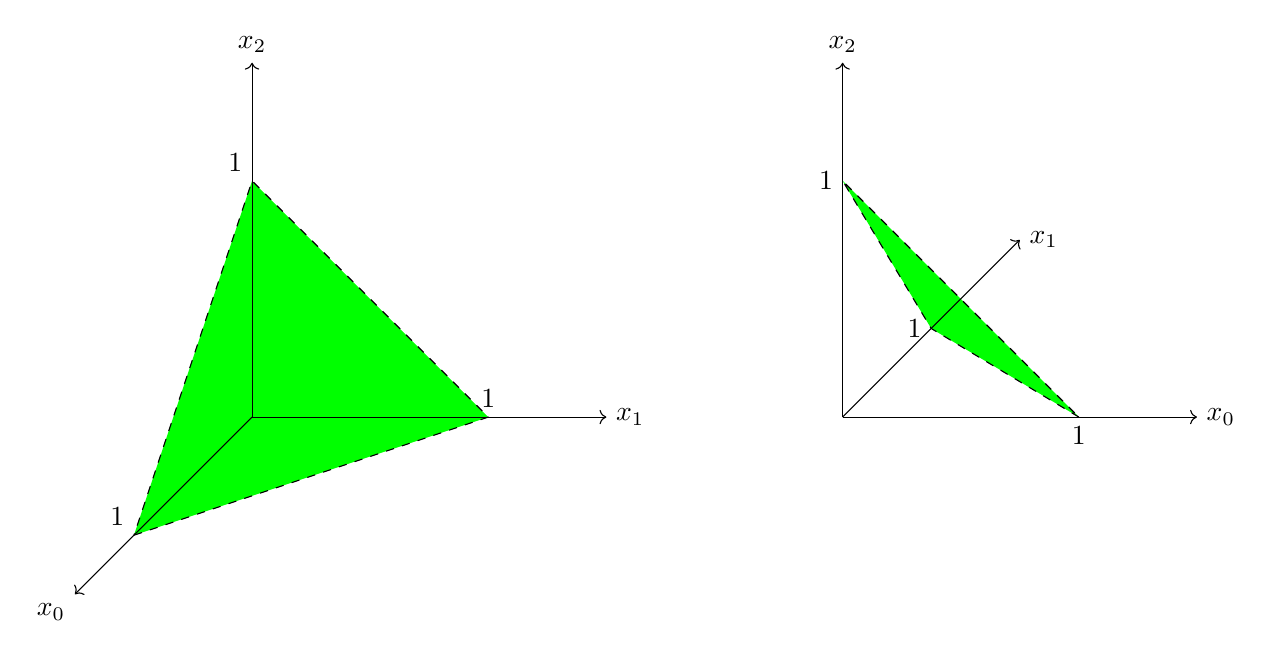
\begin{tikzpicture}[scale=0.75]
  %left
  \filldraw[dashed,fill=green]
    (-7,-2) node[above left] {$1$}
    --
    (-1,0) node[above] {$1$}
    --
    (-5,4) node[above left] {$1$}
    --
    cycle;
  \draw[->]
    (-5,0)
    --
    (-8,-3) node[below left] {$x_{0}$};
  \draw[->]
    (-5,0)
    --
    (1,0) node[right] {$x_{1}$};
  \draw[->]
    (-5,0)
    --
    (-5,6) node[above] {$x_{2}$};

  %right
  \filldraw[dashed,fill=green]
    (9,0) node[below] {$1$}
    --
    (6.5,1.5) node[left] {$1$}
    --
    (5,4) node[left] {$1$}
    --
    cycle;
  \draw[->]
    (5,0)
    --
    (11,0) node[right] {$x_{0}$};
  \draw[->]
    (5,0)
    --
    (8,3) node[right] {$x_{1}$};
  \draw[->]
    (5,0)
    --
    (5,6) node[above] {$x_{2}$};
\end{tikzpicture}
\caption{The standard simplex in dimension $0$ (top), $1$ (middle) and $2$ (bottom)}
\label{fig:stdsmplx}
\end{figure}
\\
The \textbf{face opposing $e_{i}$} in the $n$-dimensional standard simplex is - again as a subspace -
\begin{align*}
  \blacktriangle_{i}^{[n-1]}
  &:=
  \left\lbrace
      \sum_{j=0}^{n}
      x_{j}e_{j}
      \in
      \blacktriangle^{[n]}
    \colon
      x_{i}
      =
      0
  \right\rbrace
\end{align*}
It is obvious that there is a homeomorphism
\begin{align*}
  \delta_{i}^{n-1}
  \colon
  \blacktriangle^{[n-1]}
  &\to
  \blacktriangle_{i}^{[n-1]}
\end{align*}
and how it can be defined\footnote{keeping the ordering of the vertices}. We are now able to define \textbf{singular $n$-simplices} in a topological space $X$. These are just continuous maps
\begin{align*}
  \sigma
  \colon
  \blacktriangle^{[n]}
  &\to
  X
\end{align*}
and we let them be the elements of a set $S_{n}(X)$. To avoid case analysis we set $S_{n}(X) = \emptyset$ for $n < 0$. The set $S_{n}(X)$ can be turned into a free abelian group by the covariant functor $F$ assigning the set its free object
\begin{align*}
  C_{n}(X)
  &:=
  F(S_{n}(X))
\end{align*}
in $\mathbf{Ab}$. Next, for $\sigma \in S_{n}(X)$ define
\begin{align*}
  \partial_{n}(\sigma)
  &:=
  \sum_{i=0}^{n}
  (-1)^{i}
  \sigma
  \circ
  \delta_{i}^{n-1}
  \in
  C_{n-1}(X)
\end{align*}
Then $\partial_{n}$ can be (uniquely) extended to a morphism in $\mathbf{Ab}$, which is, for simplicity, again called $\partial_{n}$. It is straightforward to show that
\begin{align*}
  \partial_{n-1}
  \circ
  \partial_{n}
  &=
  0
\end{align*}
Hence $((C_{n}(X)),(\partial_{n}))$ is a chain complex. For a map $f \colon X_{1} \to X_{2}$ we define
\begin{align*}
  S_{n}(f)(\sigma)
  &:=
  f
  \circ
  \sigma
  \in S_{n}(X_{2})
\end{align*}
for $\sigma \in S_{n}(X_{1})$. Again, $S_{n}(f)$ can be (uniquiely) extended to a morphism $C_{n}(f) \colon C_{n}(X_{1}) \to C_{n}(X_{2})$ in $\mathbf{Ab}$. The idea developed here can be expanded to pairs of topological spaces, that is, elements $(X,A)$ of $\mathrm{ob}_{\mathbf{Top_{2}}}$ in the following way: set\footnote{note that if $A = \emptyset$ then $C_{n}(A)$ is trivial and thus $C_{n}((X,\emptyset))$ can be identified with $C_{n}(X)$}
\begin{align*}
  C_{n}((X,A))
  &:=
  C_{n}(X)
  /
  C_{n}(A)
\end{align*}
Since $\partial_{n}(C_{n}(A)) \subset C_{n-1}(A)$, a morphism
\begin{align*}
  \tilde{\partial}_{n}
  \colon
  C_{n}((X,A))
  &\to
  C_{n-1}((X,A))
  ,\quad
  [c]
  \mapsto
  [\partial_{n}c]
\end{align*}
in $\mathbf{Ab}$ is induced by $\partial_{n}$ which in abuse of notation is again called $\partial_{n}$. It is then immediate that $((C_{n}((X,A))),(\partial_{n}))$ is a chain complex. In a similiar vein
\begin{align*}
  C_{n}(f)
  &\colon
  C_{n}((X_{1},A_{1}))
  \to
  C_{n}((X_{2},A_{2}))
\end{align*}
is defined. Hence there is covariant functor $C$ from $\mathbf{Top_{2}}$ to $\mathbf{CC}$ which assigns to $(X,A)$ the chain complex $((C_{n}((X,A))),(\partial_{n}))$ and to $f \colon (X_{1},A_{1}) \to (X_{2},A_{2})$ the chain map $(C_{n}(f))$. The natural idea is to compose the functor $C$ with the homology group functors $H_{n}$ in order to get a homology theory. (HT2) is then immediate from the exact sequence of chain complexes
\begin{equation*}
\begin{tikzcd}[row sep=2.2em,column sep=2.6em]
  0
  \ar{r}
  &
  C((A,\emptyset))
  \ar{r}
  &
  C((X,\emptyset))
  \ar{r}
  &
  C((X,A))
  \ar{r}
  &
  0
\end{tikzcd}
\end{equation*}
The verification of the other axioms is a rather long story and therefore omitted here.\footnote{for brevity we have presented a {\glqq}Bourbaki-style{\grqq}-version of homology but actually (co)homology can be presented in a pretty intuitive way by considering CW-complexes as is done in \cite{8b5861fc}} Now singular cohomology is just the dualized version of singular homology with respect to some abelian group $G$, that is, $C$ becomes a contravariant functor $C^{\prime}$ by dualizing the constructed chain complex to a cochain complex and then $C^{\prime}$ is composed with $H^{n}$.




\chapter*{Appendix B:\quad Morse Theory}
\label{sec:morseth}
\stepcounter{prpcounter}
%\nocite{e6be9f07}
%%%
For the sake of completeness and because it is mentioned here and there in the text we briefly want to sketch the basic idea of Morse theory. We do not give any proofs here and for a more thorough introduction we refer the reader to \cite{e6be9f07}.
\\\\
The aim of Morse theory is to study differentiable real-valued functions on a manifold in order to gain information about the topology of the manifold. To illustrate this let us consider a mountainous landscape $M$ and the function $f \colon M \to \mathbb{R}$ taking every point of $M$ to its elevation over some fixed height, say sea level. Such a landscape has basins, mountain passes and peaks, or put differently minima, saddles and maxima. Now imagine the landscape is flooded with water in such a way that the water level is the same everywhere, say by rising sea level and heavy rain due to climate change. Admittedly, this is a bit artificial as there may be points lying under sea level which are not covered with water but we suppose that this does not happen because the rain is perfectly well-orchestrated. Anyway, consider the part of the landscape which is covered with water when the water level is at height $a \in \mathbb{R}$, given by
\begin{align*}
  M^{a}
  &:=
  f^{-1}
  \left(
    (-\infty,a]
  \right)
\end{align*}
The question now is, how does the topology of $M^{a}$ change when the water rises, i.e. when $a$ changes? Well, so long as no basin is filled, no mountain pass is covered and no peak is exceeded there does not seem to be any change in topology. But as soon as the water level passes one of these critical points - they really are critical points in the sense that the differential of $f$ vanishes here - there is a change in topology. When a peak is submerged then a hole in $M^{a}$ is closed, when a basin is filled then a {\glqq}bowl{\grqq} appears and when a pass is exceeded then a big hole is made into two.
\\
To get a better feeling for different kinds of critical points we consider another example. Let $M$ be a torus standing upright as illustrated in figure \ref{fig:torus}. Let moreover $f \colon M \to \mathbb{R}$ be the function taking every point to its height, i.e. the projection to the vertical axis in figure \ref{fig:torus}. The labelled points in figure \ref{fig:torus} are the critical points of $f$, that is, the points where the differential vanishes.
\begin{figure}[h!]
\centering
\begin{tikzpicture}[thick]
  % inner ellipse
  \draw[rotate around={32:(0,0)}] (0,0) ellipse (1cm and 1.5cm);
  % outer ellipse
  \draw[rotate around={30:(0,0)}] (0,0) ellipse (4.3cm and 5cm);

  % criticl points
  \fill (0,4.6) circle (1mm);
  \node[at={(0.2,4.4)}]{$h$};
  \draw[thin,dashed] (0,1.7) circle (1mm);
  \node[at={(0.35,1.45)}]{$m_{2}$};
  \fill (0,-1.6) circle (1mm);
  \node[at={(0.35,-1.85)}]{$m_{1}$};
  \draw[thin,dashed] (0,-4.3) circle (1mm);
  \node[at={(0.2,-4.5)}]{$l$};

  % coordinate axes
  \draw (0,0) -- (0,1.3);
  \draw[->] (0,4.6) -- (0,6);
  \draw (0,0) -- (-10:1.16cm);
  \draw[->] (-10:4.3cm) -- (-10:6cm);
\end{tikzpicture}
\caption{A torus standing upright and the critical points for the height function}
\label{fig:torus}
\end{figure}
We again consider how the topology of
\begin{align*}
  M^{a}
  &:=
  f^{-1}
  \left(
    (-\infty,a]
  \right)
\end{align*}
changes when $a \in \mathbb{R}$ varies. If $a$ is smaller than the height of the lowest point of the torus, labelled $l$ in figure \ref{fig:torus}, then $M^{a}$ is empty. When $a$ surpasses the lowest point, $a > l$, then $M^{a}$ starts becoming a bowl. Further increasing $a$ does not change the topology if the point where the inner hole of the torus begins is not exceeded, i.e. for $l < a < m_{1}$ with $m_{1}$ as in figure \ref{fig:torus}. But for $a > m_{1}$ and so long as $a < m_{2}$, i.e. so long as the height of the hole is not exceeded, we can describe $M^{a}$ as a cylinder with both ends bent upwards. This is homotopy equivalent to the bowl with a handle (a line segment here) attached to two points of the edge of the bowl. For $m_{2} < a < h$, i.e. when the hole is surpassed but not the full height $h$ of the torus, we have a torus with a cap cut off for $M^{a}$. This is homotopy equivalent to the cylinder with a handle attached, where the ends of the handle are attached to the two circles limiting the holes of the cylinder. Finally if $a > h$ then $M^{a}$ is the whole torus and for greater $a$ there is no more change of course. In summary we can say that the topology does not change unless a critical point is surpassed and if a critical point is surpassed then there is a cell attached to the previous object. But there are different cells attached for different critical points: at $l$ a single point, i.e. a $0$-cell, is attached to the empty set, at the middle points $m_{1},m_{2}$ a $1$-cell is attached and at $h$ a cap, i.e. a $2$-cell, is attached. But how do these critical points differ? Well, the lowest point is a minimum, i.e. here $f$ increases in either direction along the torus. The middle points are saddles, i.e. here $f$ increases in one direction and decreases in the other direction. Finally, the highest point is a maximum, thus here $f$ decreases in either direction.
\\\\
We want to capture this more formally. To this end let $M$ be an $n$-manifold, smooth as always here, and let $f \colon M \to \mathbb{R}$ a smooth function. A point $p \in M$ is a \textbf{critical point} if the differential at this point is zero, $T_{p}f = 0$. For a critical point $p$ let $\varphi \colon U \to O$ be a chart around $p$ with $\varphi(p) = 0$. Further write
\begin{align*}
  (v_{1},\ldots,v_{n})
  &:=
  T_{p}\varphi(v)
  \in
  T_{0}O
  \cong
  \mathbb{R}^{n}
\end{align*}
for $v \in T_{p}M$. Then consider the map
\begin{align*}
  T_{p}M
  \times
  T_{p}M
  &\to
  \mathbb{R}
  ,\qquad
  (v,w)
  \mapsto
  \sum_{i,j=1}^{n}
  \left(
    \partial_{i}
    \partial_{j}
    (f \circ \varphi^{-1})
  \right)
  (0)
  v_{i}
  w_{j}
\end{align*}
Now since
\begin{align*}
  \partial_{i}
  \partial_{j}
  (f \circ \varphi^{-1})
  &=
  \partial_{j}
  \partial_{i}
  (f \circ \varphi^{-1})
\end{align*}
for $1 \leq i,j \leq n$ the above map is a symmetric bilinear form on $T_{p}M$. One can moreover show that any other chart around $p$ which takes $p$ to $0$ defines the same symmetric bilinear form in this way. Note however that this is only true because $p$ is a critical point. Thus for a critical point we call the above symmetric bilinear form the \textbf{Hessian of $f$ at $p$} and denote it $\mathrm{Hess}_{p}(f)$. For any basis $\lbrace b_{1},\ldots,b_{n} \rbrace$ of $T_{p}M$ we obtain a symmetric matrix with entries
\begin{align*}
  A_{ij}
  &=
  \mathrm{Hess}_{p}(f)
  (b_{i},b_{j})
\end{align*}
In particular, for the basis coming from a coordinate chart $\varphi$ around $p$ as above this is just the matrix of second partial derivatives of $f \circ \varphi^{-1}$ at $0$. Now the symmetric matrices for different bases may have different eigenvalues. However, let $n_{0}$ be the geometric multiplicity of the eigenvalue $0$, $n_{+}$ the total geometric multiplicity of the positive eigenvalues, i.e. the sum of the dimensions of all eigenspaces for the positive eigenvalues, and likewise for $n_{-}$. Then $n_{0}$, $n_{+}$ and $n_{-}$ are independent of the chosen basis according to Sylvester's law of inertia. We call $n_{0}$ the \textbf{nullity}, $n_{+}$ the \textbf{positive index} and $n_{-}$ the \textbf{negative index}. As every matrix representing the bilinear form is symmetric we have
\begin{align*}
  n
  &=
  n_{0}
  +
  n_{+}
  +
  n_{-}
\end{align*}
We call $\mathrm{Hess}_{p}(f)$ \textbf{non-degenerate} if\footnote{this is not the standard definition for non-degeneracy of a bilinear form but for symmetric bilinear forms it is equivalent to the standard definition} $n_{0} = 0$. In this case the critical point $p$ of $f$ is also called \textbf{non-degenerate}.
\\
With these preparations we define that for an $n$-manifold $M$ a smooth function $f \colon M \to \mathbb{R}$ is a \textbf{Morse function} if every critical point of $f$ is non-degenerate. Moreover, for a critical point $p$ of $f$ the \textbf{index $\lambda(p)$ of $p$} is the negative index $n_{-}$ of the Hessian $\mathrm{Hess}_{p}(f)$. Intuitively this index of the critical point corresponds to the number of directions in which $f$ decreases from $p$. In the example of the torus above the point $l$ has index $0$, $m_{1}$ and $m_{2}$ have index $1$ and the point $h$ has index $2$. A naturally arising question is how many Morse functions there are for a manifold, if any. The answer is: there always are Morse functions and in fact, at least for compact manifolds, there is not only one Morse function but {\glqq}almost all{\grqq} functions are Morse functions. More precisely, when endowing the set $C^{\infty}(M,\mathbb{R})$ of smooth real-valued functions on compact $M$ with the Whitney $C^{2}$-topology then the Morse functions form an open and dense subset.
\\
A first important result in Morse theory is the following
\\
\begin{lem}[Morse lemma]
\label{lem:morselem}
Let $M$ be an $n$-manifold and $f \colon M \to \mathbb{R}$ a smooth function. Further let $p$ a non-degenerate critical point of $f$. Then there exists a chart $(U,\varphi)$ around $p$ with $\varphi(p) = 0$, written as
\begin{align*}
  \varphi
  &=
  \left(
    \varphi_{1}
    ,
    \ldots
    ,
    \varphi_{n}
  \right)
  \qquad
  \text{with appropriate}
  \qquad
  \varphi_{i}
  \colon
  U
  \to
  \varphi_{i}(U)
  \subset
  \mathbb{R}
\end{align*}
such that
\begin{align*}
  f(x)
  &=
  f(p)
  -
  \sum_{i=1}^{\lambda(p)}
  \varphi_{i}(x)^{2}
  +
  \sum_{i=\lambda(p)+1}^{n}
  \varphi_{i}(x)^{2}
\end{align*}
for all $x \in U$. Writing
\begin{align*}
  \left(
    y_{1}
    ,
    \ldots
    ,
    y_{n}
  \right)
  &:=
  \left(
    \varphi_{1}(x)
    ,
    \ldots
    ,
    \varphi_{n}(x)
  \right)
\end{align*}
for $y := \varphi(x) \in \varphi(U)$ we thus have
\begin{align*}
  f(\varphi^{-1}(y))
  &=
  f(\varphi^{-1}(0))
  -
  \sum_{i=1}^{\lambda(p)}
  y_{i}^{2}
  +
  \sum_{i=\lambda(p)+1}^{n}
  y_{i}^{2}
\end{align*}
for all $y \in \varphi(U)$. 
\end{lem}
As a corollary we see that non-degenerate critical points are isolated.
\\
\begin{cor}
\label{cor:ndcrisol}
Let $M$ be an $n$-manifold and $f \colon M \to \mathbb{R}$ a smooth function. Then for a non-degenerate critical point $p$ theire exists a neighbourhood of $p$ in $M$ which contains no other critical point than $p$. Thus if $f$ is a Morse function, the set of non-degenerate critical points is discrete.
\end{cor}
Now for $a \in \mathbb{R}$ and smooth $f \colon M \to \mathbb{R}$ define
\begin{align*}
  M^{a}
  &:=
  f^{-1}
  \left(
    (-\infty,a]
  \right)
\end{align*}
which is manifold with boundary if $f^{-1}(\lbrace a \rbrace)$ contains no critical point. Then we have the following two fundamental theorems describing how $M^{a}$ changes as $a$ varies.
\\
\begin{thm}
\label{thm:morsenocrit}
Let $f \colon M \to \mathbb{R}$ a smooth map on an $n$-manifold $M$ and let $a < b \in \mathbb{R}$. If $f^{-1}([a,b])$ is compact and contains no critical points of $f$ then $M^{a}$ is diffeomorphic to $M^{b}$ and $M^{a}$ is a deformation retract of $M^{b}$.
\end{thm}
\begin{thm}
\label{thm:morseonecrit}
Let $f \colon M \to \mathbb{R}$ a smooth map on an $n$-manifold $M$, let $p \in M$ be a critical point of $f$ and set $c := f(p)$. Suppose there is $\varepsilon > 0$ such that $f^{-1}([c-\varepsilon,c+\varepsilon])$ is compact and contains no critical points of $f$ besides $p$. Then $M^{c+\varepsilon}$ is homotopy equivalent to $M^{c-\varepsilon}$ with a $\lambda(p)$-dimensional cell $D^{\lambda(p)}$ attached, i.e. to
\begin{align*}
  M^{c-\varepsilon}
  \cup_{g}
  D^{\lambda(p)}
\end{align*}
where
\begin{align*}
  g
  \colon
  \partial
  D^{\lambda(p)}
  &\to
  M^{c-\varepsilon}
\end{align*}
is some attaching map.
\end{thm}
The idea for attaching the cell in the latter theorem \ref{thm:morseonecrit} is to choose a chart according to the Morse lemma \ref{lem:morselem} and attach the cell to the part of $M^{c-\varepsilon}$ with vanishing coordinates for $i > \lambda(p)$.
\\
With the help of the two above theorems one can show the following
\\
\begin{thm}
\label{thm:mancw}
Let $f \colon M \to \mathbb{R}$ a Morse function on an $n$-manifold $M$. If $M^{a}$ is compact for each $a \in \mathbb{R}$ then $M$ is homotopy equivalent to a CW-complex with one cell of dimension $\lambda$ for each critical point with index $\lambda$.
\end{thm}
From the above results we see that a Morse function provides a way of decomposing a manifold. But different Morse functions may yield different decompositions and the question then is how these decompositions are related. This can be examined with Cerf theory where one studies families of smooth functions, or more precisely paths between two Morse functions in the space of smooth functions. Therefore people sometimes also speak of paramaterized Morse theory. We do not go into further detail here but refer the reader to the literature and conclude our description of Morse theory.




\chapter*{Appendix C:\quad Detailed Proofs from Chapter \ref{CHAP:ALTCHARPROPS}}
\label{chap:detailproofs}
\stepcounter{prpcounter}
Here we give the detailed proofs left out in chapter \ref{CHAP:ALTCHARPROPS}. As already announced there we will often suppress the tensor product symbol between objects in diagrams and longer expressions and we will make heavy use of the coherence theorem for (symmetric) monoidal categories. Remember that we often simply write $\sim$ for unique isomorphisms guaranteed by the coherence theorem, possibly indexed by natural numbers like $\sim_{2}$. Again, all diagrams in this chapter are supposed to be commutative unless stated otherwise, as we will often make changes in diagrams and justify why the diagrams still commute without explicitly saying that they commute.



\section*{Lemma \ref{LEM:DUALOBTENSOR}}
\label{sec:lemdualobtensor}
\begin{lem}
\label{lem:appdualobtensor}
Let $\mathbf{C}$ be a monoidal category and let $X_{1},X_{2} \in \mathrm{ob}_{\mathbf{C}}$ have left dual objects $X_{1}^{\prime},X_{2}^{\prime}$ with coevaluations $\mathrm{coev}_{X_{1}},\mathrm{coev}_{X_{2}}$ and evaluations $\mathrm{ev}_{X_{1}},\mathrm{ev}_{X_{2}}$, respectively. Then $X_{2}^{\prime} \otimes X_{1}^{\prime}$ is a left dual object of $X_{1} \otimes X_{2}$ where the coevaluation is given by
\begin{equation*}
\begin{tikzcd}[row sep=3.2em,column sep=8em]
  1
  \ar{rr}{\mathrm{coev}_{X_{1} X_{2}}}
  \ar{d}[swap]{\mathrm{coev}_{X_{1}}}
  &
  &
  (X_{1} X_{2}) (X_{2}^{\prime} X_{1}^{\prime})
  \\
  X_{1} X_{1}^{\prime}
  \ar{r}{\mathsf{R}^{-1}(X_{1}) \otimes \mathrm{id}_{X_{1}^{\prime}}}
  &
  (X_{1} 1) X_{1}^{\prime}
  \ar{r}{(\mathrm{id}_{X_{1}} \otimes \mathrm{coev}_{X_{2}}) \otimes \mathrm{id}_{X_{1}^{\prime}}}
  &
  (X_{1} (X_{2} X_{2}^{\prime})) X_{1}^{\prime}
  \ar{u}[swap]{i_{\mathsf{A}}^{(c)}}
\end{tikzcd}
\end{equation*}
and the evaluation is given by
\begin{equation*}
\begin{tikzcd}[row sep=3.2em,column sep=8em]
  (X_{2}^{\prime} X_{1}^{\prime}) (X_{1} X_{2})
  \ar{rr}{\mathrm{ev}_{X_{1} X_{2}}}
  \ar{d}[swap]{i_{\mathsf{A}}^{(e)}}
  &
  &
  1
  \\
  X_{2}^{\prime} ((X_{1}^{\prime} X_{1}) X_{2})
  \ar{r}{\mathrm{id}_{X_{2}^{\prime}} \otimes (\mathrm{ev}_{X_{1}} \otimes \mathrm{id}_{X_{2}})}
  &
  X_{2}^{\prime} (1 X_{2})
  \ar{r}{\mathrm{id}_{X_{2}^{\prime}} \otimes \mathsf{L}(X_{2})}
  &
  X_{2}^{\prime} X_{2}
  \ar{u}[swap]{\mathrm{ev}_{X_{2}}}
\end{tikzcd}
\end{equation*}
with $i_{\mathsf{A}}^{(c)}$ and $i_{\mathsf{A}}^{(e)}$ the corresponding unique\footnote{the uniqueness is guaranteed by the coherence theorem} isomorphisms built from the associator.
\\
In the case of a symmetric monoidal category the coevaluation and the evaluation can be written as
\begin{equation*}
\begin{tikzcd}[row sep=3.2em,column sep=8em]
  1
  \ar{r}{\mathrm{coev}_{X_{1} X_{2}}}
  \ar{d}[swap]{\mathsf{R}^{-1}(1)}
  &
  (X_{1} X_{2}) (X_{2}^{\prime} X_{1}^{\prime})
  \\
  1 1
  \ar{r}{\mathrm{coev}_{X_{1}} \otimes \mathrm{coev}_{X_{2}}}
  &
  (X_{1} X_{1}^{\prime}) (X_{2} X_{2}^{\prime})
  \ar{u}[swap]{i^{(c)}}
\end{tikzcd}
\end{equation*}
and
\begin{equation*}
\begin{tikzcd}[row sep=3.2em,column sep=8em]
  (X_{2}^{\prime} X_{1}^{\prime}) (X_{1} X_{2})
  \ar{r}{\mathrm{ev}_{X_{1} X_{2}}}
  \ar{d}[swap]{i^{(e)}}
  &
  1
  \\
  (X_{1}^{\prime} X_{1}) (X_{2}^{\prime} X_{2})
  \ar{r}{\mathrm{ev}_{X_{1}} \otimes \mathrm{ev}_{X_{2}}}
  &
  1 1
  \ar{u}[swap]{\mathsf{L}(1)}
\end{tikzcd}
\end{equation*}
where $i^{(c)}$ and $i^{(e)}$ are the corresponding unique isomorphisms built from the associator and the braiding.
\end{lem}
\begin{prf}
With the coherence theorem we find from the definitions that the outer perimeter of the following diagram commutes. The small inner parts commutes because of the naturality of $\mathsf{A}$.
\begin{equation*}
\hspace{-2em}
\begin{tikzcd}[row sep=5.5em,column sep=3.5em,font=\footnotesize,every label/.append style={font=\tiny}]
  ((X_{1} X_{2}) (X_{2}^{\prime} X_{1}^{\prime})) (X_{1} X_{2})
  \ar{rr}{\mathsf{A}(X_{1} X_{2},X_{2}^{\prime} X_{1}^{\prime},X_{1} X_{2})}
  &
  &
  (X_{1} X_{2}) ((X_{2}^{\prime} X_{1}^{\prime}) (X_{1} X_{2}))
  \ar{d}[description,xshift=3mm]{\mathrm{id}_{X_{1} X_{2}} \otimes \mathrm{ev}_{X_{1} X_{2}}}
  \\
  1 (X_{1} X_{2})
  \ar{u}[description,xshift=-3mm]{\mathrm{coev}_{X_{1} X_{2}} \otimes \mathrm{id}_{X_{1} X_{2}}}
  \ar{d}[description,xshift=-2mm]{\mathsf{A}^{-1}(1,X_{1},X_{2})}
  &
  &
  (X_{1} X_{2}) 1
  \\
  (1 X_{1}) X_{2}
  \ar{d}[description,xshift=-2mm]{\mathsf{A}(1,X_{1},X_{2})}
  \ar{r}{(\mathrm{coev}_{X_{1}} \otimes \mathrm{id}_{X_{1}}) \otimes \mathrm{id}_{X_{2}}}
  &
  ((X_{1} X_{1}^{\prime}) X_{1}) X_{2}
  \ar{ddl}[description,xshift=4mm,yshift=4mm]{\mathsf{A}(X_{1} X_{1}^{\prime},X_{1},X_{2})}
  &
  X_{1} (X_{2} 1)
  \ar{u}[description,xshift=2mm]{\mathsf{A}^{-1}(X_{1},X_{2},1)}
  \\
  1 (X_{1} X_{2})
  \ar{d}[description,xshift=-4mm]{\mathrm{coev}_{X_{1}} \otimes \mathrm{id}_{X_{1} X_{2}}}
  &
  &
  (X_{1} X_{2}) 1
  \ar{u}[description,xshift=3mm]{\mathsf{A}(X_{1},X_{2},1)}
  \\
  (X_{1} X_{1}^{\prime}) (X_{1} X_{2})
  \ar{d}[description,xshift=-5mm]{(\mathsf{R}^{-1}(X_{1}) \otimes \mathrm{id}_{X_{1}^{\prime}}) \otimes \mathrm{id}_{X_{1} X_{2}}}
  &
  X_{1} (X_{2} (X_{2}^{\prime} X_{2}))
  \ar{uur}[description,xshift=-4mm,yshift=-5mm]{\mathrm{id}_{X_{1}} \otimes (\mathrm{id}_{X_{2}} \otimes \mathrm{ev}_{X_{2}})}
  &
  (X_{1} X_{2}) (X_{2}^{\prime} X_{2})
  \ar{u}[description,xshift=3mm]{\mathrm{id}_{X_{1} X_{2}} \otimes \mathrm{ev}_{X_{2}}}
  \ar{l}{\mathsf{A}(X_{1},X_{2},X_{2}^{\prime} X_{2})}
  \\
  ((X_{1} 1) X_{1}^{\prime}) (X_{1} X_{2})
  \ar{r}{\mathsf{A}(X_{1} 1,X_{1}^{\prime},(X_{1} X_{2}))}
  \ar{d}[description,xshift=-4mm]{((\mathrm{id}_{X_{1}} \otimes \mathrm{coev}_{X_{2}}) \otimes \mathrm{id}_{X_{1}^{\prime}}) \otimes \mathrm{id}_{X_{1} X_{2}}}
  &
  (X_{1} 1) (X_{1}^{\prime} (X_{1} X_{2}))
  \ar{ddl}[description,xshift=11mm,yshift=5mm]{(\mathrm{id}_{X_{1}} \otimes \mathrm{coev}_{X_{2}}) \otimes \mathrm{id}_{X_{1}^{\prime} (X_{1} X_{2})}}
  &
  (X_{1} X_{2}) (X_{2}^{\prime} (1 X_{2}))
  \ar{u}[description,xshift=4mm]{\mathrm{id}_{X_{1} X_{2}} \otimes (\mathrm{id}_{X_{2}^{\prime}} \otimes \mathsf{L}(X_{2}))}
  \\
  ((X_{1} (X_{2} X_{2}^{\prime})) X_{1}^{\prime}) (X_{1} X_{2})
  \ar{d}[description,xshift=-4mm]{\mathsf{A}(X_{1} (X_{2} X_{2}^{\prime}),X_{1}^{\prime},(X_{1} X_{2}))}
  &
  &
  (X_{1} X_{2}) (X_{2}^{\prime} ((X_{1}^{\prime} X_{1}) X_{2}))
  \ar{u}[description,xshift=7mm,yshift=-4mm]{\mathrm{id}_{X_{1} X_{2}} \otimes (\mathrm{id}_{X_{2}^{\prime}} \otimes (\mathrm{ev}_{X_{1}} \otimes \mathrm{id}_{X_{2}}))}
  \\
  (X_{1} (X_{2} X_{2}^{\prime})) (X_{1}^{\prime} (X_{1} X_{2}))
  \ar{rd}[swap]{\mathsf{id}_{X_{1} (X_{2} X_{2}^{\prime})} \otimes \mathsf{A}^{-1}(X_{1}^{\prime},X_{1},X_{2})}
  &
  ((X_{1} X_{2}) X_{2}^{\prime}) (1 X_{2})
  \ar{uur}[description,xshift=-7mm,yshift=-5mm]{\mathsf{A}(X_{1} X_{2},X_{2}^{\prime},1 X_{2})}
  &
  ((X_{1} X_{2}) X_{2}^{\prime}) ((X_{1}^{\prime} X_{1}) X_{2})
  \ar{u}[description,xshift=5mm]{\mathsf{A}(X_{1} X_{2},X_{2}^{\prime},(X_{1}^{\prime} X_{1}) X_{2})}
  \ar{l}[swap,xshift=1mm,yshift=2pt]{\mathrm{id}_{(X_{1} X_{2}) X_{2}^{\prime}} \otimes (\mathrm{ev}_{X_{1}} \otimes \mathrm{id}_{X_{2}})}
  \\
  &
  (X_{1} (X_{2} X_{2}^{\prime})) ((X_{1}^{\prime} X_{1}) X_{2})
  \ar{ur}[swap]{\mathsf{A}^{-1}(X_{1},X_{2},X_{2}^{\prime}) \otimes \mathrm{id}_{(X_{1}^{\prime} X_{1}) X_{2}}}
  &
\end{tikzcd}
\end{equation*}
We go the inner way and use the functoriality of the tensor product for the four lowermost arrows to obtain the following diagram. The small inner parts commute due to the coherence theorem.
\begin{equation*}
\hspace{-2em}
\begin{tikzcd}[row sep=5.5em,column sep=2.5em,font=\footnotesize,every label/.append style={font=\tiny}]
  ((X_{1} X_{2}) (X_{2}^{\prime} X_{1}^{\prime})) (X_{1} X_{2})
  \ar{rrr}{\mathsf{A}(X_{1} X_{2},X_{2}^{\prime} X_{1}^{\prime},X_{1} X_{2})}
  &
  &
  &
  (X_{1} X_{2}) ((X_{2}^{\prime} X_{1}^{\prime}) (X_{1} X_{2}))
  \ar{d}[description,xshift=4mm]{\mathrm{id}_{X_{1} X_{2}} \otimes \mathrm{ev}_{X_{1} X_{2}}}
  \\
  1 (X_{1} X_{2})
  \ar{u}[description,xshift=-4mm]{\mathrm{coev}_{X_{1} X_{2}} \otimes \mathrm{id}_{X_{1} X_{2}}}
  \ar{d}[description,xshift=-4mm]{\mathsf{A}^{-1}(1,X_{1},X_{2})}
  &
  &
  &
  (X_{1} X_{2}) 1
  \\
  (1 X_{1}) X_{2}
  \ar{d}[description,xshift=-4mm]{(\mathrm{coev}_{X_{1}} \otimes \mathrm{id}_{X_{1}}) \otimes \mathrm{id}_{X_{2}}}
  &
  &
  &
  X_{1} (X_{2} 1)
  \ar{u}[description,xshift=4mm]{\mathsf{A}^{-1}(X_{1},X_{2},1)}
  \\
  ((X_{1} X_{1}^{\prime}) X_{1}) X_{2}
  \ar{rd}{\mathsf{A}(X_{1},X_{1}^{\prime},X_{1}) \otimes \mathrm{id}_{X_{2}}}
  \ar{d}[description,xshift=-5mm]{\mathsf{A}(X_{1} X_{1}^{\prime},X_{1},X_{2})}
  &
  &
  &
  X_{1} (X_{2} (X_{2}^{\prime} X_{2}))
  \ar{u}[description,xshift=4mm]{\mathrm{id}_{X_{1}} \otimes (\mathrm{id}_{X_{2}} \otimes \mathrm{ev}_{X_{2}})}
  \\
  (X_{1} X_{1}^{\prime}) (X_{1} X_{2})
  \ar{d}[description,xshift=-4mm]{(\mathsf{R}^{-1}(X_{1}) \otimes \mathrm{id}_{X_{1}^{\prime}}) \otimes \mathrm{id}_{X_{1} X_{2}}}
  &
  (X_{1} (X_{1}^{\prime} X_{1})) X_{2}
  \ar{d}[description,xshift=3mm]{(\mathsf{R}^{-1}(X_{1}) \otimes \mathrm{id}_{X_{1}^{\prime} X_{1}}) \otimes \mathrm{id}_{X_{2}}}
  &
  &
  (X_{1} X_{2}) (X_{2}^{\prime} X_{2})
  \ar{u}[description,xshift=4mm]{\mathsf{A}(X_{1},X_{2},X_{2}^{\prime} X_{2})}
  \\
  ((X_{1} 1) X_{1}^{\prime}) (X_{1} X_{2})
  \ar{d}[description,xshift=-4mm]{\mathsf{A}(X_{1} 1,X_{1}^{\prime},(X_{1} X_{2}))}
  &
  ((X_{1} 1) (X_{1}^{\prime} X_{1})) X_{2}
  \ar{ddl}{\mathsf{A}(X_{1} 1,X_{1}^{\prime} X_{1},X_{2})}
  &
  X_{1} ((X_{2} X_{2}^{\prime}) X_{2})
  \ar{uur}{\mathrm{id}_{X_{1}} \otimes \mathsf{A}(X_{2},X_{2}^{\prime},X_{2})}
  &
  (X_{1} X_{2}) (X_{2}^{\prime} (1 X_{2}))
  \ar{u}[description,xshift=4mm]{\mathrm{id}_{X_{1} X_{2}} \otimes (\mathrm{id}_{X_{2}^{\prime}} \otimes \mathsf{L}(X_{2}))}
  \\
  (X_{1} 1) (X_{1}^{\prime} (X_{1} X_{2}))
  \ar{d}[description,xshift=-5.5mm,yshift=3mm]{\mathsf{id}_{X_{1} 1} \otimes \mathsf{A}^{-1}(X_{1}^{\prime},X_{1},X_{2})}
  &
  &
  X_{1} ((X_{2} X_{2}^{\prime}) (1 X_{2}))
  \ar{u}[description,xshift=-4mm]{\mathrm{id}_{X_{1}} \otimes (\mathrm{id}_{X_{2} X_{2}^{\prime}} \otimes \mathsf{L}(X_{2}))}
  &
  ((X_{1} X_{2}) X_{2}^{\prime}) (1 X_{2})
  \ar{u}[description,xshift=4mm]{\mathsf{A}(X_{1} X_{2},X_{2}^{\prime},1 X_{2})}
  \\
  (X_{1} 1) ((X_{1}^{\prime} X_{1}) X_{2})
  \ar{rrd}[swap]{\mathrm{id}_{X_{1} 1} \otimes (\mathrm{ev}_{X_{1}} \otimes \mathrm{id}_{X_{2}})}
  &
  &
  &
  (X_{1} (X_{2} X_{2}^{\prime})) (1 X_{2})
  \ar{u}[description,xshift=4mm]{\mathsf{A}^{-1}(X_{1},X_{2},X_{2}^{\prime}) \otimes \mathrm{id}_{1 X_{2}}}
  \ar{ul}{\mathsf{A}(X_{1},X_{2} X_{2}^{\prime},1 X_{2})}
  \\
  &
  &
  (X_{1} 1) (1 X_{2})
  \ar{ur}[swap]{(\mathrm{id}_{X_{1}} \otimes \mathrm{coev}_{X_{2}}) \otimes \mathrm{id}_{1 X_{2}}}
  &
\end{tikzcd}
\end{equation*}
\newpage
Again going the inner way yields the following outer diagram. Here the lower inner small parts on the left and right are the naturality of $\mathsf{A}$ and the middle inner small parts on the left and right commute due to the functoriality of the tensor product. Moreover the upper inner small parts on the left and right are diagram (LD1) governing dual objects for $X_{1}, X_{1}^{\prime}$ and $X_{2}, X_{2}^{\prime}$, respectively. Finally the central inner part follows from the coherence theorem.
\begin{equation*}
\hspace{-2em}
\begin{tikzcd}[row sep=5.8em,column sep=3.1em,font=\footnotesize,every label/.append style={font=\tiny}]
  ((X_{1} X_{2}) (X_{2}^{\prime} X_{1}^{\prime})) (X_{1} X_{2})
  \ar{rrr}{\mathsf{A}(X_{1} X_{2},X_{2}^{\prime} X_{1}^{\prime},X_{1} X_{2})}
  &
  &
  &
  (X_{1} X_{2}) ((X_{2}^{\prime} X_{1}^{\prime}) (X_{1} X_{2}))
  \ar{d}[description,xshift=4mm]{\mathrm{id}_{X_{1} X_{2}} \otimes \mathrm{ev}_{X_{1} X_{2}}}
  \\
  1 (X_{1} X_{2})
  \ar{u}[description,xshift=-4mm]{\mathrm{coev}_{X_{1} X_{2}} \otimes \mathrm{id}_{X_{1} X_{2}}}
  \ar{rr}{\mathsf{L}(X_{1} X_{2})}
  \ar{d}[description,xshift=-5mm]{\mathsf{A}^{-1}(1,X_{1},X_{2})}
  &
  &
  X_{1} X_{2}
  \ar{r}{\mathsf{R}^{-1}(X_{1} X_{2})}
  &
  (X_{1} X_{2}) 1
  \\
  (1 X_{1}) X_{2}
  \ar{rd}{\mathsf{L}(X_{1}) \otimes \mathrm{id}_{X_{2}}}
  \ar{d}[description,xshift=-4mm]{(\mathrm{coev}_{X_{1}} \otimes \mathrm{id}_{X_{1}}) \otimes \mathrm{id}_{X_{2}}}
  &
  &
  &
  X_{1} (X_{2} 1)
  \ar{u}[description,xshift=5mm]{\mathsf{A}^{-1}(X_{1},X_{2},1)}
  \\
  ((X_{1} X_{1}^{\prime}) X_{1}) X_{2}
  \ar{d}[description,xshift=-4mm]{\mathsf{A}(X_{1},X_{1}^{\prime},X_{1}) \otimes \mathrm{id}_{X_{2}}}
  &
  X_{1} X_{2}
  \ar{d}[description]{\mathsf{R}^{-1}(X_{1}) \otimes \mathrm{id}_{X_{2}}}
  &
  X_{1} X_{2}
  \ar{ur}{\mathrm{id}_{X_{1}} \otimes \mathsf{R}^{-1}(X_{2})}
  &
  X_{1} (X_{2} (X_{2}^{\prime} X_{2}))
  \ar{u}[description,xshift=4mm]{\mathrm{id}_{X_{1}} \otimes (\mathrm{id}_{X_{2}} \otimes \mathrm{ev}_{X_{2}})}
  \\
  (X_{1} (X_{1}^{\prime} X_{1})) X_{2}
  \ar{r}[yshift=3pt]{(\mathrm{id}_{X_{1}} \otimes \mathrm{ev}_{X_{1}}) \otimes \mathrm{id}_{X_{2}}}
  \ar{d}[description,xshift=-4mm]{(\mathsf{R}^{-1}(X_{1}) \otimes \mathrm{id}_{X_{1}^{\prime} X_{1}}) \otimes \mathrm{id}_{X_{2}}}
  &
  (X_{1} 1) X_{2}
  \ar{d}[description,xshift=-4mm]{(\mathsf{R}^{-1}(X_{1}) \otimes \mathrm{id}_{1}) \otimes \mathrm{id}_{X_{2}}}
  &
  X_{1} (1 X_{2})
  \ar{u}[description]{\mathrm{id}_{X_{1}} \otimes \mathsf{L}(X_{2})}
  \ar{r}[yshift=3pt]{\mathrm{id}_{X_{1}} \otimes (\mathrm{coev}_{X_{2}} \otimes \mathrm{id}_{X_{2}})}
  &
  X_{1} ((X_{2} X_{2}^{\prime}) X_{2})
  \ar{u}[description,xshift=4mm]{\mathrm{id}_{X_{1}} \otimes \mathsf{A}(X_{2},X_{2}^{\prime},X_{2})}
  \\
  ((X_{1} 1) (X_{1}^{\prime} X_{1})) X_{2}
  \ar{r}[yshift=3pt]{(\mathrm{id}_{X_{1} 1} \otimes \mathrm{ev}_{X_{1}}) \otimes \mathrm{id}_{X_{2}}}
  \ar{d}[description,xshift=-5mm]{\mathsf{A}(X_{1} 1,X_{1}^{\prime} X_{1},X_{2})}
  &
  ((X_{1} 1) 1) X_{2}
  \ar{rdd}[swap]{\mathsf{A}(X_{1} 1,1,X_{2})}
  &
  X_{1} (1 (1 X_{2}))
  \ar{u}[description,xshift=3mm]{\mathrm{id}_{X_{1}} \otimes (\mathrm{id}_{1} \otimes \mathsf{L}(X_{2}))}
  \ar{r}[yshift=3pt]{\mathrm{id}_{X_{1}} \otimes (\mathrm{coev}_{X_{2}} \otimes \mathrm{id}_{1 X_{2}})}
  &
  X_{1} ((X_{2} X_{2}^{\prime}) (1 X_{2}))
  \ar{u}[description,xshift=4mm]{\mathrm{id}_{X_{1}} \otimes (\mathrm{id}_{X_{2} X_{2}^{\prime}} \otimes \mathsf{L}(X_{2}))}
  \\
  (X_{1} 1) ((X_{1}^{\prime} X_{1}) X_{2})
  \ar{rrd}[swap]{\mathrm{id}_{X_{1} 1} \otimes (\mathrm{ev}_{X_{1}} \otimes \mathrm{id}_{X_{2}})}
  &
  &
  &
  (X_{1} (X_{2} X_{2}^{\prime})) (1 X_{2})
  \ar{u}[description,xshift=4mm]{\mathsf{A}(X_{1},X_{2} X_{2}^{\prime},1 X_{2})}
  \\
  &
  &
  (X_{1} 1) (1 X_{2})
  \ar{uu}[swap]{\mathsf{A}(X_{1},1,1 X_{2})}
  \ar{ur}[swap]{(\mathrm{id}_{X_{1}} \otimes \mathrm{coev}_{X_{2}}) \otimes \mathrm{id}_{1 X_{2}}}
  &
\end{tikzcd}
\end{equation*}
But the upper part is precisely the first diagram (LD1) governing dual objects for $X_{1} \otimes X_{2}$ and $X_{2}^{\prime} \otimes X_{1}^{\prime}$. The commutativity of the second diagram (LD2) can be shown in the same way.
\newpage
For the second part, concerning symmetric monoidal categories, consider the following diagram whose outer perimeter is the definition of $\mathrm{coev}_{X_{1} X_{2}}$. The lower part follows from the naturality of $\mathsf{A}$. Note that we use the notation mentioned in the introduction, i.e. we write $\sim$ for unique isomorphisms built from $\mathsf{A}$, $\mathsf{L}$, $\mathsf{R}$, and $\mathsf{B}$.
\begin{equation*}
\begin{tikzcd}[row sep=5em,column sep=5em]
  1
  \ar{rrr}{\mathrm{coev}_{X_{1} X_{2}}}
  \ar{d}[swap]{\mathrm{coev}_{X_{1}}}
  &
  &
  &
  (X_{1} X_{2}) (X_{2}^{\prime} X_{1}^{\prime})
  \\
  X_{1} X_{1}^{\prime}
  \ar{d}[swap]{\mathsf{R}^{-1}(X_{1}) \otimes \mathrm{id}_{X_{1}^{\prime}}}
  &
  X_{1} (1 X_{1}^{\prime})
  \ar{rr}{\mathrm{id}_{X_{1}} \otimes (\mathrm{coev}_{X_{2}} \otimes \mathrm{id}_{X_{1}^{\prime}})}
  &
  &
  X_{1} ((X_{2} X_{2}^{\prime}) X_{1}^{\prime})
  \ar{u}[swap]{\sim}
  \\
  (X_{1} 1) X_{1}^{\prime}
  \ar{ur}[swap]{\mathsf{A}(X_{1},1,X_{1}^{\prime})}
  \ar{rrr}{(\mathrm{id}_{X_{1}} \otimes \mathrm{coev}_{X_{2}}) \otimes \mathrm{id}_{X_{1}^{\prime}}}
  &
  &
  &
  (X_{1} (X_{2} X_{2}^{\prime})) X_{1}^{\prime}
  \ar{u}[swap]{\mathsf{A}(X_{1},X_{2} X_{2}^{\prime},X_{1}^{\prime})}
\end{tikzcd}
\end{equation*}
The upper part can be rewritten the with the help of the coherence theorem for symmetric monoidal categories to obtain the outer perimeter of the following diagram. The right part is the naturality of $\mathsf{B}$, the lower part is the naturality of $\mathsf{A}$, the leftmost part is the naturality of $\mathsf{R}$ and the triangle next to it is the functoriality of the tensor product. For the upper right part the coherence theorem ensures that there is a unique isomorphism $i^{(c)}$ built from $\mathsf{A}$, $\mathsf{L}$, $\mathsf{R}$, and $\mathsf{B}$. But the upper left part is exactly what we had to show.
\begin{equation*}
\begin{tikzcd}[row sep=5em,column sep=5em]
  &
  &
  (X_{1} X_{2}) (X_{2}^{\prime} X_{1}^{\prime})
  &
  \\
  1
  \ar{urr}{\mathrm{coev}_{X_{1} X_{2}}}
  \ar{r}[swap]{\mathsf{R}^{-1}(1)}
  \ar{d}[swap]{\mathrm{coev}_{X_{1}}}
  &
  1 1
  \ar{d}[description,xshift=5mm]{\mathrm{coev}_{X_{1}} \otimes \mathrm{coev}_{X_{2}}}
  \ar{ddl}[swap,xshift=3mm,yshift=2mm]{\mathrm{coev}_{X_{1}} \otimes \mathrm{id}_{1}}
  &
  &
  X_{1} ((X_{2} X_{2}^{\prime}) X_{1}^{\prime})
  \ar{ul}[swap]{\sim}
  \\
  X_{1} X_{1}^{\prime}
  \ar{d}[swap]{\mathsf{R}^{-1}(X_{1} X_{1}^{\prime})}
  &
  (X_{1} X_{1}^{\prime}) (X_{2} X_{2}^{\prime})
  \ar[bend right=28]{uur}{i^{(c)}}
  \ar{r}{\mathsf{A}(X_{1},X_{1}^{\prime},X_{2} X_{2}^{\prime})}
  &
  X_{1} (X_{1}^{\prime} (X_{2} X_{2}^{\prime}))
  \ar{ur}{\mathrm{id}_{X_{1}} \otimes \mathsf{B}(X_{1}^{\prime},X_{2} X_{2}^{\prime})}
  &
  X_{1} (1 X_{1}^{\prime})
  \ar{u}[description,xshift=3mm]{\mathrm{id}_{X_{1}} \otimes (\mathrm{coev}_{X_{2}} \otimes \mathrm{id}_{X_{1}^{\prime}})}
  \\
  (X_{1} X_{1}^{\prime}) 1
  \ar{ur}[swap]{\mathrm{id}_{X_{1} X_{1}^{\prime}} \otimes \mathrm{coev}_{X_{2}}}
  \ar{rrr}{\mathsf{A}(X_{1},X_{1}^{\prime},1)}
  &
  &
  &
  X_{1} (X_{1}^{\prime} 1)
  \ar{u}[description,xshift=5mm]{\mathrm{id}_{X_{1}} \otimes \mathsf{B}(X_{1}^{\prime},1)}
  \ar{ul}{\mathrm{id}_{X_{1}} \otimes (\mathrm{id}_{X_{1}^{\prime}} \otimes \mathrm{coev}_{X_{2}})}
\end{tikzcd}
\end{equation*}
The diagram defining the evaluation $\mathrm{ev}_{X_{1} X_{2}}$ can be treated analogously.
\\
\phantom{proven}
\hfill
$\Box$
\end{prf}



\section*{Theorem \ref{THM:ACSMF}}
\label{sec:thmacsmf}
\begin{thm}
\label{thm:appacsmf}
Let $\mathbf{C}$, $\mathbf{C}_{\alpha}$ be symmetric monoidal categories and let $\mathbf{C}$ be left\footnote{
in fact, the category is also a right rigid, since it is braided} rigid. Let $E$ be a tuple $(E_{\mathrm{ob}},E_{\mathrm{mor}},\mathsf{H},\Phi)$ of
\begin{enumerate}
\item
a function
\begin{align*}
  E_{\mathrm{ob}}
  \colon
  \mathrm{ob}_{\mathbf{C}}
  &\to
  \mathrm{ob}_{\mathbf{C}_{\alpha}}
\end{align*}

\item
a function $E_{\mathrm{mor}}$ which maps $X \in \mathrm{ob}_{\mathbf{C}}$ to a function
\begin{align*}
  E_{\mathrm{mor}}(X)
  \colon
  \mathrm{mor}_{\mathbf{C}}(1,X)
  &\to
  \mathrm{mor}_{\mathbf{C}_{\alpha}}
  \left(
    E_{\mathrm{ob}}(1)
    ,
    E_{\mathrm{ob}}(X)
  \right)
\end{align*}

\item
a function $\mathsf{H}$ assigning to each object
\begin{align*}
  (X_{1},X_{2})
  \in
  \mathrm{ob}_{\mathbf{C} \times \mathbf{C}}
\end{align*}
an isomorphism
\begin{align*}
  \mathsf{H}(X_{1},X_{2})
  \in
  \mathrm{mor}_{\mathbf{C}_{\alpha}}
  \left(
    E_{\mathrm{ob}}(X_{1})
    \otimes_{\alpha}
    E_{\mathrm{ob}}(X_{2})
    ,
    E_{\mathrm{ob}}(X_{1} \otimes X_{2})
  \right)
\end{align*}

\item
an isomorphism
\begin{align*}
  \Phi
  \in
  \mathrm{mor}_{\mathbf{C}_{\alpha}}
  \left(
    1_{\alpha}
    ,
    E_{\mathrm{ob}}(1)
  \right)
\end{align*}
\end{enumerate}
In abuse of notation we will simply write $E$ for both $E_{\mathrm{ob}}$ and all $E_{\mathrm{mor}}(X)$. Then the following are equivalent
\begin{enumerate}
\item[i)]
$E$ extends to a symmetric monoidal functor from $\mathbf{C}$ to $\mathbf{C}_{\alpha}$

\item[ii)]
$E$ satisfies
\begin{enumerate}
\item[(AC1)]
for each $X \in \mathrm{ob}_{\mathbf{C}}$ and left dual object $X^{\prime}$ with evaluation $\mathrm{ev}_{X}$ and coevaluaton $\mathrm{coev}_{X}$ there is a morphism
\begin{align*}
  \mathrm{ev}_{E(X)}
  \in
  \mathrm{mor}_{\mathrm{C}_{\alpha}}
  \left(
    E(X^{\prime})
    \otimes_{\alpha}
    E(X)
    ,
    1_{\alpha}
  \right)
\end{align*}
which makes $E(X^{\prime})$ a left dual object of $E(X)$ with coevaluation map
\begin{align*}
  \mathrm{coev}_{E(X)}
  &:=
  \mathsf{H}(X,X^{\prime})^{-1}
  \circ
  E(\mathrm{coev}_{X})
  \circ
  \Phi
\end{align*}
Remember that this means that the following diagrams commute
\begin{equation*}
\begin{tikzcd}[row sep=3.3em,column sep=4.5em]
  1_{\alpha} E(X)
  \ar{r}{\mathsf{L}_{\alpha}(E(X))}
  \ar{d}[swap]{\mathrm{coev}_{E(X)} \otimes_{\alpha} \mathrm{id}_{E(X)}}
  &
  E(X)
  &
  E(X) 1_{\alpha}
  \ar{l}[swap]{\mathsf{R}_{\alpha}(E(X))}
  \\
  (E(X) E(X^{\prime})) E(X)
  \ar{rr}{\mathsf{A}_{\alpha}(E(X),E(X^{\prime}),E(X))}
  &
  &
  E(X) (E(X^{\prime}) E(X))
  \ar{u}[swap]{\mathrm{id}_{E(X)} \otimes_{\alpha} \mathrm{ev}_{E(X)}}
\end{tikzcd}
\end{equation*}
\begin{equation*}
\begin{tikzcd}[row sep=3.3em,column sep=4.5em]
  E(X^{\prime}) 1_{\alpha}
  \ar{r}{\mathsf{R}_{\alpha}(E(X^{\prime}))}
  \ar{d}[swap]{\mathrm{id}_{E(X^{\prime})} \otimes_{\alpha} \mathrm{coev}_{E(X)}}
  &
  E(X^{\prime})
  &
  1_{\alpha} E(X^{\prime})
  \ar{l}[swap]{\mathsf{L}_{\alpha}(E(X^{\prime}))}
  \\
  E(X^{\prime}) (E(X) E(X^{\prime}))
  \ar{rr}{\mathsf{A}_{\alpha}^{-1}(E(X^{\prime}),E(X),E(X^{\prime}))}
  &
  &
  (E(X^{\prime}) E(X)) E(X^{\prime})
  \ar{u}[swap]{\mathrm{ev}_{E(X)} \otimes_{\alpha} \mathrm{id}_{E(X^{\prime})}}
\end{tikzcd}
\end{equation*}

\item[(AC2)]
for all $X_{1},X_{2} \in \mathrm{ob}_{\mathbf{C}}$, left dual objects $X_{1}^{\prime}$ of $X_{1}$ and all
\begin{align*}
  f
  \in
  \mathrm{mor}_{\mathbf{C}}
  \left(
    1
    ,
    X_{2}
    \otimes
    (X_{1}^{\prime} \otimes X_{1})
  \right)
\end{align*}
the following diagram commutes
\begin{equation*}
\hspace{1cm}
\begin{tikzcd}[row sep=3.3em,column sep=7.5em]
  E(1)
  \ar{r}{E(\mathsf{R}(X_{2}) \circ (\mathrm{id}_{X_{2}} \otimes \mathrm{ev}_{X_{1}}) \circ f)}
  \ar{d}[swap]{E(f)}
  &
  E(X_{2})
  &
  E(X_{2}) 1_{\alpha}
  \ar{l}[swap]{\mathsf{R}_{\alpha}(E(X_{2}))}
  \\
  E(X_{2} (X_{1}^{\prime} X_{1}))
  \ar{r}{\mathsf{H}(X_{2},X_{1}^{\prime} X_{1})^{-1}}
  &
  E(X_{2}) (E(X_{1}^{\prime} X_{1}))
  \ar{r}{\mathrm{id}_{E(X_{2})} \otimes_{\alpha} \mathsf{H}(X_{1}^{\prime},X_{1})^{-1}}
  &
  E(X_{2}) (E(X_{1}^{\prime}) E(X_{1}))
  \ar{u}[swap]{\mathrm{id}_{E(X_{2})} \otimes_{\alpha} \mathrm{ev}_{E(X_{1})}}
\end{tikzcd}
\end{equation*}

\item[(AC3)]
for all
\begin{align*}
  f_{1}
  \in
  \mathrm{mor}_{\mathbf{C}}(1,X_{1})
  ,\qquad
  f_{2}
  \in
  \mathrm{mor}_{\mathbf{C}}(1,X_{2})
\end{align*}
the following diagram commutes
\begin{equation*}
\begin{tikzcd}[row sep=3.3em,column sep=8em]
  E(1)
  \ar{r}{E((f_{1} \otimes f_{2}) \circ \mathsf{L}^{-1}(1))}
  \ar{d}[swap]{\mathsf{L}_{\alpha}^{-1}(E(1))}
  &
  E(X_{1} X_{2})
  \\
  1_{\alpha} E(1)
  \ar{d}[swap]{\Phi \otimes_{\alpha} \mathrm{id}_{E(1)}}
  &
  \\
  E(1) E(1)
  \ar{r}{E(f_{1}) \otimes_{\alpha} E(f_{2})}
  &
  E(X_{1}) E(X_{2})
  \ar{uu}[swap]{\mathsf{H}(X_{1},X_{2})}
\end{tikzcd}
\end{equation*}

\item[(AC4)]
let
\begin{align*}
  X_{1}
  ,
  \ldots
  ,
  X_{n}
  \in
  \mathrm{ob}_{\mathbf{C}}
  ,\qquad
  n
  \in
  \mathbb{N}^{\times}
\end{align*}
and let $W$ be the tensor product of $X_{1},\dots,X_{n}$ in this order, with any choice of bracketing. Let $\pi \in S_{n}$ be a permutation and write $W_{\pi}$ for the tensor product of $X_{\pi(1)},\dots,X_{\pi(n)}$ in this order and with any choice of bracketing which may be different from that of $W$. There is an isomorphism
\begin{align*}
    \hat{\pi}
    \colon
    W
    &\to
    W_{\pi}
\end{align*}
built from the symmetric braiding $\mathsf{B}$ and the associator $\mathsf{A}$. This isomorphism is unique since though it can possibly be written in many ways, the coherence theorem ensures that these ways are all equal. Furthermore, let $W^{E}$ be the tensor product of $E(X_{1}),\dots,E(X_{n})$ in this order, with the same bracketing as $W$ and likewise for $W_{\pi}^{E}$ and $E(X_{\pi(1)}),\dots,E(X_{\pi(n)})$. We denote the corresponding unique isomorphism by
\begin{align*}
  \hat{\pi}_{\alpha}
  \colon
  W^{E}
  &\to
  W_{\pi}^{E}
\end{align*}
Additionally, we write
\begin{align*}
  \mathsf{H}^{W}
  \colon
  W^{E}
  &\to
  E(W)
\end{align*}
for the isomorphism obtained by subsequent applicaton of $\mathsf{H}$ (tensored with appropriate identities) and analogously for
\begin{align*}
  \mathsf{H}_{\pi}^{W}
  \colon
  W_{\pi}^{E}
  &\to
  E(W_{\pi})
\end{align*}
Then for $f \in \mathrm{mor}_{\mathbf{C}}(1,W)$ the following diagram commutes
\begin{equation*}
\begin{tikzcd}[row sep=3.3em,column sep=large]
  E(1)
  \ar{rr}{E(\hat{\pi} \circ f)}
  \ar{d}[swap]{E(f)}
  &
  &
  E(W_{\pi})
  \\
  E(W)
  \ar{r}{\mathsf{H}^{W -1}}
  &
  W^{E}
  \ar{r}{\hat{\pi}_{\alpha}}
  &
  W_{\pi}^{E}
  \ar{u}[swap]{\mathsf{H}_{\pi}^{W}}
\end{tikzcd}
\end{equation*}

\item[(AC5)]
for the unit object the equation
\begin{align*}
  E(\mathrm{id}_{1})
  &=
  \mathrm{id}_{E(1)}
\end{align*}
holds and the following diagrams commute
\begin{equation*}
\begin{tikzcd}[row sep=3.3em,column sep=4em]
  1_{\alpha} E(1)
  \ar{r}{\mathsf{L}_{\alpha}(E(1))}
  \ar{d}[swap]{\Phi \otimes_{\alpha} \mathrm{id}_{E(1)}}
  &
  E(1)
  \\
  E(1) E(1)
  \ar{r}{\mathsf{H}(1,1)}
  &
  E(1 1)
  \ar{u}[swap]{E(\mathsf{L}(1))}
\end{tikzcd}
\qquad
\begin{tikzcd}[row sep=3.3em,column sep=4em]
  E(1) 1_{\alpha}
  \ar{r}{\mathsf{R}_{\alpha}(E(1))}
  \ar{d}[swap]{\mathrm{id}_{E(1)} \otimes_{\alpha} \Phi}
  &
  E(1)
  \\
  E(1) E(1)
  \ar{r}{\mathsf{H}(1,1)}
  &
  E(1 1)
  \ar{u}[swap]{E(\mathsf{R}(1))}
\end{tikzcd}
\end{equation*}
\end{enumerate}
The extension to a symmetric monoidal functor in i) is unique if $E$ satisfies the conditions in ii).
\end{enumerate}
\end{thm}
\begin{prf}
The proof is not too difficult but quite tedious as it involves a lot of dealing with the associators, unit laws and braidings and the diagrams in (AC1) - (AC5).
\\\\
i) $\Rightarrow$ ii)
\qquad
This direction is rather immediate. We denote the symmetric monoidal functor which is an extension of $(E,\mathsf{H},\Phi)$ by $(F,\mathsf{H},\Phi)$ and define the dual pairing to be
\begin{align*}
  \mathrm{ev}_{E(X)}
  &:=
  \Phi^{-1}
  \circ
  F(\mathrm{ev}_{X})
  \circ
  \mathsf{H}(X^{\prime},X)
  \colon
  F(X^{\prime})
  \otimes_{\alpha}
  F(X)
  \to
  1_{\alpha}
\end{align*}
The diagrams in (AC1) are just lemma \ref{lem:mfduals}. We leave the rest out as the other conditions can be checked fairly easily: for (AC2) and (AC3) one uses the functoriality of $F$, (MF2) and the naturality of $\mathsf{H}$; (AC4) follows by the functoriality of $F$ and multiple application of (MF1) and (BF); (AC5) is just functoriality of $F$ and a special case of (MF2).
\\\\
ii) $\Rightarrow$ i)
\qquad
This part is a rather long story. Set $F_{\mathrm{ob}} := E_{\mathrm{ob}}$. We have to extend $E$ to all morphisms in $\mathbf{C}$. To this end we need a left dual object $X^{\prime}$ for every object $X \in \mathrm{ob}_{\mathbf{C}}$. We know that $\mathbf{C}$ is left rigid, so these dual objects exist and we can suppose that there is a choice function to choose them or that they have been constructed explicitly. Either way, we choose $1^{\prime} = 1$ with
\begin{align*}
  \mathrm{coev}_{1}
  &=
  \mathsf{L}^{-1}(1)
  =
  \mathsf{R}^{-1}(1)
  \\
  \mathrm{ev}_{1}
  &=
  \mathsf{L}(1)
  =
  \mathsf{R}(1)
\end{align*}
and for tensor products we take dual objects as given by lemma \ref{LEM:DUALOBTENSOR}. Now for
\begin{align*}
  f_{12}
  \in
  \mathrm{mor}_{\mathbf{C}}(X_{1},X_{2})
\end{align*}
define
\begin{align*}
  \tilde{f}_{12}
  &:=
  \left(
    f_{12}
    \otimes
    \mathrm{id}_{X_{1}^{\prime}}
  \right)
  \circ
  \mathrm{coev}_{X_{1}}
  \colon
  1
  \to
  X_{2}
  \otimes
  X_{1}^{\prime}
  \\
  \gamma_{f_{12}}
  &:=
  \mathsf{H}(X_{2},X_{1}^{\prime})^{-1}
  \circ
  E(\tilde{f}_{12})
  \circ
  \Phi
  \colon
  1_{\alpha}
  \to
  E(X_{2})
  \otimes
  E(X_{1}^{\prime})
\end{align*}
Then we let $F_{\mathrm{mor}}$ be the function that maps
\begin{align*}
  (X_{1},X_{2})
  \in
  \mathrm{ob}_{\mathbf{C}}
  \times
  \mathrm{ob}_{\mathbf{C}}
\end{align*}
to the function
\begin{align*}
  F_{\mathrm{mor}}(X_{1},X_{2})
  \colon
  \mathrm{mor}_{\mathbf{C}}(X_{1},X_{2})
  &\to
  \mathrm{mor}_{\mathbf{C}_{\alpha}}(F_{\mathrm{ob}}(X_{1}),F_{\mathrm{ob}}(X_{2}))
\end{align*}
defined by the following commuting diagram
\begin{equation*}
\begin{tikzcd}[row sep=3.2em,column sep=10em]
  E(X_{1})
  \ar{r}{F_{\mathrm{mor}}(X_{1},X_{2})(f_{12})}
  \ar{d}[swap]{\mathsf{L}_{\alpha}^{-1}(E(X_{1}))}
  &
  E(X_{2})
  \\
  1_{\alpha} E(X_{1})
  \ar{d}[swap]{\gamma_{f_{12}} \otimes_{\alpha} \mathrm{id}_{E(X_{1})}}
  &
  E(X_{2}) 1_{\alpha}
  \ar{u}[swap]{\mathsf{R}_{\alpha}(E(X_{2}))}
  \\
  (E(X_{2}) E(X_{1}^{\prime})) E(X_{1})
  \ar{r}{\mathsf{A}_{\alpha}(E(X_{2}),E(X_{1}^{\prime}),E(X_{1}))}
  &
  E(X_{2}) (E(X_{1}^{\prime}) E(X_{1}))
  \ar{u}[swap]{\mathrm{id}_{E(X_{2})} \otimes_{\alpha} \mathrm{ev}_{E(X_{1})}}
\end{tikzcd}
\end{equation*}
Again we will write $F$ for both $F_{\mathrm{ob}}$ and all $F_{\mathrm{mor}}(X_{1},X_{2})$.
\\\\
We need to check that $F$ actually extends $E$, i.e. that for $g \in \mathrm{mor}_{\mathbf{C}}(1,Y)$ we have
\begin{align*}
  F(g)
  &=
  E(g)
\end{align*}
We know
\begin{align*}
  \tilde{g}
  &=
  (g \otimes \mathrm{id}_{1})
  \circ
  \mathsf{L}^{-1}(1)
\end{align*}
thus (AC3) yields
\begin{align*}
  E(\tilde{g})
  &=
  \mathsf{H}(Y,1)
  \circ
  \left(
    E(g)
    \otimes_{\alpha}
    \mathrm{id}_{E(1)}
  \right)
  \circ
  \left(
    \Phi
    \otimes_{\alpha}
    \mathrm{id}_{E(1)}
  \right)
  \circ
  \mathsf{L}_{\alpha}^{-1}(E(1))
  \\
  \Rightarrow
  \qquad
  \gamma_{g}
  &=
  \left(
    E(g)
    \otimes_{\alpha}
    \mathrm{id}_{E(1)}
  \right)
  \circ
  \left(
    \Phi
    \otimes_{\alpha}
    \mathrm{id}_{E(1)}
  \right)
  \circ
  \mathsf{L}_{\alpha}^{-1}(E(1))
  \circ
  \Phi
  \\
  &=
  \left(
    E(g)
    \otimes_{\alpha}
    \mathrm{id}_{E(1)}
  \right)
  \circ
  \mathsf{H}(1,1)^{-1}
  \circ
  E(\mathsf{L}^{-1}(1))
  \circ
  \Phi
  \\
  &=
  \left(
    E(g)
    \otimes_{\alpha}
    \mathrm{id}_{E(1)}
  \right)
  \circ
  \mathrm{coev}_{E(1)}
\end{align*}
Note that for the second last equality we used (AC3) with $f_{1} = f_{2} = \mathrm{id}_{1}$ and moreover we used $E(\mathrm{id}_{1}) = \mathrm{id}_{E(1)}$ from (AC5). Hence we have the outer perimeter of the following diagram
\begin{equation*}
\begin{tikzcd}[row sep=3.8em,column sep=6em]
  E(1)
  \ar{rr}{F(g)}
  \ar{rd}{\mathrm{id}_{E(1)}}
  \ar{d}[swap]{\mathsf{L}_{\alpha}^{-1}(E(1))}
  &
  &
  E(Y)
  \\
  1_{\alpha} E(1)
  \ar{dd}[swap]{\mathrm{coev}_{E(1)} \otimes_{\alpha} \mathrm{id}_{E(1)}}
  &
  E(1)
  \ar{ur}{E(g)}
  &
  \\
  &
  E(1) 1_{\alpha}
  \ar{u}[swap]{\mathsf{R}_{\alpha}(E(1))}
  \ar{r}{E(g) \otimes_{\alpha} \mathrm{id}_{1_{\alpha}}}
  &
  E(Y) 1_{\alpha}
  \ar{uu}[swap]{\mathsf{R}_{\alpha}(E(Y))}
  \\
  (E(1) E(1)) E(1)
  \ar{r}{\mathsf{A}_{\alpha}(E(1),E(1),E(1))}
  \ar{d}[swap]{(E(g) \otimes_{\alpha} \mathrm{id}_{E(1)}) \otimes_{\alpha} \mathrm{id}_{E(1)}}
  &
  E(1) (E(1) E(1))
  \ar{u}[swap]{\mathrm{id}_{E(1)} \otimes_{\alpha} \mathrm{ev}_{E(1)}}
  \ar{rd}{E(g) \otimes_{\alpha} \mathrm{id}_{E(1) E(1)}}
  &
  \\
  (E(Y) E(1)) E(1)
  \ar{rr}{\mathsf{A}_{\alpha}(E(Y),E(1),E(1))}
  &
  &
  E(Y) (E(1) E(1))
  \ar{uu}[swap]{\mathrm{id}_{E(Y)} \otimes_{\alpha} \mathrm{ev}_{E(1)}}
\end{tikzcd}
\end{equation*}
Here the lower left part is the naturality of $\mathsf{A}_{\alpha}$, the lower right part is the functoriality of $\otimes_{\alpha}$ and the upper right part is the naturality of $\mathsf{R}_{\alpha}$. Moreover the first diagram from (AC1) makes the upper left part commute and therefore the upper central part commutes which means that $F(g) = E(g)$.
\\\\
Next, we have to verify that $(F,\mathsf{H},\Phi)$ is a symmetric monoidal functor from $\mathbf{C}$ to $\mathbf{C}_{\alpha}$. We verify the properties step by step.
\begin{enumerate}
\item[(F1)]
\begin{align*}
  \mathrm{F}(\mathrm{id}_{X})
  &=
  \mathrm{id}_{F(X)}
\end{align*}
follows immediately from (AC1) since
\begin{align*}
  \widetilde{\mathrm{id}}_{X}
  &=
  \mathrm{coev}_{X}
\end{align*}
implying that
\begin{align*}
  \gamma_{\mathrm{id}_{X}}
  &=
  \mathsf{H}(X,X^{\prime})^{-1}
  \circ
  E(\mathrm{coev}_{X})
  \circ
  \Phi
  \\
  &=
  \mathrm{coev}_{E(X)}
\end{align*}

\item[(F2)]
\begin{align*}
  F(f_{23} \circ f_{12})
  &=
  F(f_{23}) \circ F(f_{12})
\end{align*}
for
\begin{align*}
  f_{12} \in \mathrm{mor}_{\mathbf{C}}(X_{1},X_{2})
  ,\qquad
  f_{23} \in \mathrm{mor}_{\mathbf{C}}(X_{2},X_{3})
\end{align*}
needs a rather lengthy calculation. We will do this by making subsequent changes in commuting diagrams to obtain new commuting diagrams using the conditions (AC2) - (AC4), the coherence theorem and the naturality of the associators, the unit laws and the braidings. Additionally the functoriality of the tensor products is used, often without explicitly saying it. To further ease notation we define
\begin{align*}
  E_{i}
  &:=
  E(X_{i})
  ,\qquad
  E_{i}^{\prime}
  :=
  E(X_{i}^{\prime})
  ,\qquad
  1
  \leq
  i
  \leq
  4
\end{align*}
By definition we have the upper part of the following diagram, where the lower part commutes by the coherence theorem.
\begin{equation*}
\hspace{-2em}
\begin{tikzcd}[row sep=3.2em,column sep=5em]
  E_{1}
  \ar{r}{F(f_{12})}
  \ar{d}[swap]{\mathsf{L}_{\alpha}^{-1}(E_{1})}
  &
  E_{2}
  \ar{r}{F(f_{23})}
  &
  E_{3}
  \\
  1_{\alpha} E_{1}
  \ar{d}[swap]{\gamma_{f_{12}} \otimes_{\alpha} \mathrm{id}_{E_{1}}}
  &
  &
  E_{3} 1_{\alpha}
  \ar{u}[swap]{\mathsf{R}_{\alpha}(E_{3})}
  \\
  (E_{2} E_{1}^{\prime}) E_{1}
  \ar{d}[swap]{\mathsf{A}_{\alpha}(E_{2},E_{1}^{\prime},E_{1})}
  &
  &
  E_{3} (E_{2}^{\prime} E_{2})
  \ar{u}[swap]{\mathrm{id}_{E_{3}} \otimes_{\alpha} \mathrm{ev}_{E_{2}}}
  \\
  E_{2} (E_{1}^{\prime} E_{1})
  \ar{d}[swap]{\mathrm{id}_{E_{2}} \otimes_{\alpha} \mathrm{ev}_{E_{1}}}
  &
  &
  (E_{3} E_{2}^{\prime}) E_{2}
  \ar{u}[swap]{\mathsf{A}_{\alpha}(E_{3},E_{2}^{\prime},E_{2})}
  \\
  E_{2} 1_{\alpha}
  \ar{r}{\mathsf{R}_{\alpha}(E_{2})}
  \ar{d}[swap]{\mathsf{L}_{\alpha}^{-1}(E_{2}) \otimes_{\alpha} \mathrm{id}_{1_{\alpha}}}
  &
  E_{2}
  \ar{r}{\mathsf{L}_{\alpha}^{-1}(E_{2})}
  &
  1_{\alpha} E_{2}
  \ar{u}[swap]{\gamma_{f_{23}} \otimes_{\alpha} \mathrm{id}_{E_{2}}}
  \\
  (1_{\alpha} E_{2}) 1_{\alpha}
  \ar{rr}{\mathsf{A}_{\alpha}(1_{\alpha},E_{2},1_{\alpha})}
  &
  &
  1_{\alpha} (E_{2} 1_{\alpha})
  \ar{u}[swap]{\mathrm{id}_{1_{\alpha}} \otimes_{\alpha} \mathsf{R}_{\alpha}(E_{2})}
\end{tikzcd}
\end{equation*}
With the functoriality of $\otimes_{\alpha}$ we can rewrite the outer perimeter as the following outer perimeter and also obtain the lower left part. The lower right part is the naturality of $\mathsf{A}_{\alpha}$.
\begin{equation*}
\hspace{-2em}
\begin{tikzcd}[row sep=4.5em,column sep=7.5em]
  E_{1}
  \ar{r}{F(f_{12})}
  \ar{d}[swap]{\mathsf{L}_{\alpha}^{-1}(E_{1})}
  &
  E_{2}
  \ar{r}{F(f_{23})}
  &
  E_{3}
  \\
  1_{\alpha} E_{1}
  \ar{d}[swap]{\gamma_{f_{12}} \otimes_{\alpha} \mathrm{id}_{E_{1}}}
  &
  &
  E_{3} 1_{\alpha}
  \ar{u}[swap]{\mathsf{R}_{\alpha}(E_{3})}
  \\
  (E_{2} E_{1}^{\prime}) E_{1}
  \ar{d}[swap]{\mathsf{A}_{\alpha}(E_{2},E_{1}^{\prime},E_{1})}
  &
  ((E_{3} E_{2}^{\prime}) E_{2}) (E_{1}^{\prime} E_{1})
  \ar{dd}{\mathrm{id}_{(E_{3} E_{2}^{\prime}) E_{2}} \otimes_{\alpha} \mathrm{ev}_{E_{1}}}
  &
  E_{3} (E_{2}^{\prime} E_{2})
  \ar{u}[swap]{\mathrm{id}_{E_{3}} \otimes_{\alpha} \mathrm{ev}_{E_{2}}}
  \\
  E_{2} (E_{1}^{\prime} E_{1})
  \ar{d}[swap]{\mathsf{L}_{\alpha}^{-1}(E_{2}) \otimes_{\alpha} \mathrm{id}_{E_{1}^{\prime} E_{1}}}
  &
  &
  (E_{3} E_{2}^{\prime}) E_{2}
  \ar{u}[swap]{\mathsf{A}_{\alpha}(E_{3},E_{2}^{\prime},E_{2})}
  \\
  (1_{\alpha} E_{2}) (E_{1}^{\prime} E_{1})
  \ar{uur}[swap,xshift=-6mm,yshift=-4mm]{(\gamma_{f_{23}} \otimes_{\alpha} \mathrm{id}_{E_{2}}) \otimes_{\alpha} \mathrm{id}_{E_{1}^{\prime} E_{1}}}
  \ar{d}[swap]{\mathrm{id}_{1_{\alpha} E_{2}} \otimes_{\alpha} \mathrm{ev}_{E_{1}}}
  &
  ((E_{3} E_{2}^{\prime}) E_{2}) 1_{\alpha}
  \ar{r}{\mathsf{A}_{\alpha}(E_{3} E_{2}^{\prime},E_{2},1_{\alpha})}
  &
  (E_{3} E_{2}^{\prime}) (E_{2} 1_{\alpha})
  \ar{u}[swap]{\mathrm{id}_{E_{3} E_{2}^{\prime}} \otimes_{\alpha} \mathsf{R}_{\alpha}(E_{2})}
  \\
  (1_{\alpha} E_{2}) 1_{\alpha}
  \ar{ur}[swap]{(\gamma_{f_{23}} \otimes_{\alpha} \mathrm{id}_{E_{2}}) \otimes_{\alpha} \mathrm{id}_{1_{\alpha}}}
  \ar{rr}{\mathsf{A}_{\alpha}(1_{\alpha},E_{2},1_{\alpha})}
  &
  &
  1_{\alpha} (E_{2} 1_{\alpha})
  \ar{u}[swap]{\gamma_{f_{23}} \otimes_{\alpha} \mathrm{id}_{E_{2} 1_{\alpha}}}
\end{tikzcd}
\end{equation*}
The coherence theorem allows us to rewrite the upper part as the outer perimeter of the following diagram. The parts on the lower left and right follow from the naturality of $\mathsf{A}_{\alpha}$ and the lower central part is the unique isomorphism guranteed by the coherence theorem. The parts on the upper left and right are the naturality of $\mathsf{L}_{\alpha}$ and $\mathsf{R}_{\alpha}$, respectively, and the triangles next to them commute due to the functoriality of the tensor product.
\begin{equation*}
\hspace{-1.8em}
\begin{tikzcd}[row sep=7em,column sep=5em,font=\footnotesize,every label/.append style={font=\tiny}]
  E_{1}
  \ar{r}{F(f_{12})}
  \ar{d}[swap]{\mathsf{L}_{\alpha}^{-1}(E_{1})}
  &
  E_{2}
  \ar{rr}{F(f_{23})}
  &
  &
  E_{3}
  \\
  1_{\alpha} E_{1}
  \ar{rd}{\mathsf{L}_{\alpha}^{-1}(1_{\alpha}) \otimes_{\alpha} \mathrm{id}_{E_{1}}}
  \ar{d}[description,xshift=-4mm]{\gamma_{f_{12}} \otimes_{\alpha} \mathrm{id}_{E_{1}}}
  &
  &
  &
  E_{3} 1_{\alpha}
  \ar{u}[swap]{\mathsf{R}_{\alpha}(E_{3})}
  \\
  (E_{2} E_{1}^{\prime}) E_{1}
  \ar{d}[description,xshift=-3mm]{\mathsf{L}_{\alpha}^{-1}(E_{2} E_{1}^{\prime}) \otimes_{\alpha} \mathrm{id}_{E_{1}}}
  &
  (1_{\alpha} 1_{\alpha}) E_{1}
  \ar{dd}[description,xshift=3mm]{(\gamma_{f_{23}} \otimes_{\alpha} \gamma_{f_{12}}) \otimes_{\alpha} \mathrm{id}_{E_{1}}}
  \ar{dl}[description,xshift=2mm,yshift=4mm]{(\mathrm{id}_{1_{\alpha}} \otimes_{\alpha} \gamma_{f_{12}}) \otimes_{\alpha} \mathrm{id}_{E_{1}}}
  &
  E_{3} (1_{\alpha} 1_{\alpha})
  \ar{ur}{\mathrm{id}_{E_{3}} \otimes_{\alpha} \mathsf{R}_{\alpha}(1_{\alpha})}
  &
  E_{3} (E_{2}^{\prime} E_{2})
  \ar{u}[description,xshift=4mm]{\mathrm{id}_{E_{3}} \otimes_{\alpha} \mathrm{ev}_{E_{2}}}
  \\
  (1_{\alpha} (E_{2} E_{1}^{\prime})) E_{1}
  \ar{rd}[description,yshift=-4mm]{(\gamma_{f_{23}} \otimes_{\alpha} \mathrm{id}_{E_{2} E_{1}^{\prime}}) \otimes_{\alpha} \mathrm{id}_{E_{1}}}
  \ar{d}[description,xshift=-3mm,yshift=4mm]{\mathsf{A}_{\alpha}^{-1}(1_{\alpha},E_{2},E_{1}^{\prime}) \otimes_{\alpha} \mathrm{id}_{E_{1}}}
  &
  &
  E_{3} ((E_{2}^{\prime} E_{2}) (E_{1}^{\prime} E_{1}))
  \ar{u}[description,xshift=-3mm,yshift=-2mm]{\mathrm{id}_{E_{3}} \otimes_{\alpha} (\mathrm{ev}_{E_{2}} \otimes_{\alpha} \mathrm{ev}_{E_{1}})}
  \ar{r}[xshift=-3mm,yshift=3pt]{\mathrm{id}_{E_{3}} \otimes_{\alpha} (\mathrm{id}_{E_{2}^{\prime} E_{2}} \otimes_{\alpha} \mathrm{ev}_{E_{1}})}
  &
  E_{3} ((E_{2}^{\prime} E_{2}) 1_{\alpha})
  \ar{u}[description,xshift=3mm]{\mathrm{id}_{E_{3}} \otimes_{\alpha} \mathsf{R}_{\alpha}(E_{2}^{\prime} E_{2})}
  \ar{ul}[description,xshift=-2mm,yshift=5mm]{\mathrm{id}_{E_{3}} \otimes_{\alpha} (\mathrm{ev}_{E_{2}} \otimes_{\alpha} \mathrm{id}_{1_{\alpha}})}
  \\
  ((1_{\alpha} E_{2}) E_{1}^{\prime}) E_{1}
  \ar{rd}[description,xshift=2mm,yshift=-4mm]{((\gamma_{f_{23}} \otimes_{\alpha} \mathrm{id}_{E_{2}}) \otimes_{\alpha} \mathrm{id}_{E_{1}^{\prime}}) \otimes_{\alpha} \mathrm{id}_{E_{1}}}
  \ar{d}[description,xshift=-2mm,yshift=3mm]{\mathsf{A}_{\alpha}(1_{\alpha} E_{2},E_{1}^{\prime},E_{1})}
  &
  ((E_{3} E_{2}^{\prime}) (E_{2} E_{1}^{\prime})) E_{1}
  \ar{ur}{\sim}
  \ar{d}[description,yshift=5mm]{\mathsf{A}_{\alpha}^{-1}(E_{3} E_{2}^{\prime},E_{2},E_{1}^{\prime}) \otimes_{\alpha} \mathrm{id}_{E_{1}}}
  &
  E_{3} (E_{2}^{\prime} (E_{2} (E_{1}^{\prime} E_{1})))
  \ar{u}[description,xshift=3mm]{\mathrm{id}_{E_{3}} \otimes_{\alpha} \mathsf{A}_{\alpha}^{-1}(E_{2}^{\prime},E_{2},E_{1}^{\prime} E_{1})}
  \ar{r}[xshift=-2mm,yshift=3pt]{\mathrm{id}_{E_{3}} \otimes_{\alpha} (\mathrm{id}_{E_{2}^{\prime}} \otimes_{\alpha} (\mathrm{id}_{E_{2}} \otimes_{\alpha} \mathrm{ev}_{E_{1}}))}
  &
  E_{3} (E_{2}^{\prime} (E_{2} 1_{\alpha}))
  \ar{u}[description,xshift=2mm]{\mathrm{id}_{E_{3}} \otimes_{\alpha} \mathsf{A}_{\alpha}^{-1}(E_{2}^{\prime},E_{2},1_{\alpha})}
  \\
  (1_{\alpha} E_{2}) (E_{1}^{\prime} E_{1})
  \ar{d}[description,xshift=-1mm,yshift=-2mm]{(\gamma_{f_{23}} \otimes_{\alpha} \mathrm{id}_{E_{2}}) \otimes_{\alpha} \mathrm{id}_{E_{1}^{\prime} E_{1}}}
  &
  (((E_{3} E_{2}^{\prime}) E_{2}) E_{1}^{\prime}) E_{1}
  \ar{dl}[description,xshift=4mm,yshift=5mm]{\mathsf{A}_{\alpha}((E_{3} E_{2}^{\prime}) E_{2},E_{1}^{\prime},E_{1})}
  &
  (E_{3} E_{2}^{\prime}) (E_{2} (E_{1}^{\prime} E_{1}))
  \ar{u}[description,xshift=2mm]{\mathsf{A}_{\alpha}(E_{3},E_{2}^{\prime},E_{2} (E_{1}^{\prime} E_{1}))}
  \ar{r}[yshift=3pt]{\mathrm{id}_{E_{3} E_{2}^{\prime}} \otimes_{\alpha} (\mathrm{id}_{E_{2}} \otimes_{\alpha} \mathrm{ev}_{E_{1}})}
  &
  (E_{3} E_{2}^{\prime}) (E_{2} 1_{\alpha})
  \ar{u}[description,xshift=3mm]{\mathsf{A}_{\alpha}(E_{3},E_{2}^{\prime},E_{2} 1_{\alpha})}
  \\
  ((E_{3} E_{2}^{\prime}) E_{2}) (E_{1}^{\prime} E_{1})
  \ar{urr}[swap]{\mathsf{A}_{\alpha}(E_{3} E_{2}^{\prime},E_{2},E_{1}^{\prime} E_{1})}
  \ar{rrr}{(\mathrm{id}_{E_{3} E_{2}^{\prime}} \otimes_{\alpha} \mathrm{id}_{E_{2}}) \otimes_{\alpha} \mathrm{ev}_{E_{1}}}
  &
  &
  &
  ((E_{3} E_{2}^{\prime}) E_{2}) 1_{\alpha}
  \ar{u}[description,xshift=3mm]{\mathsf{A}_{\alpha}(E_{3} E_{2}^{\prime},E_{2},1_{\alpha})}
\end{tikzcd}
\end{equation*}
Going the upper central way and using the definition of the $\gamma_{f_{ij}}$ we find the outer perimeter of the following diagram where the small inner part is the naturality of $\mathsf{L}_{\alpha}$.
\begin{equation*}
\hspace{-1em}
\begin{tikzcd}[row sep=3.2em,column sep=6em]
  E_{1}
  \ar{r}{F(f_{12})}
  \ar{d}[swap]{\mathsf{L}_{\alpha}^{-1}(E_{1})}
  &
  E_{2}
  \ar{r}{F(f_{23})}
  &
  E_{3}
  \\
  1_{\alpha} E_{1}
  \ar{rd}{\Phi \otimes_{\alpha} \mathrm{id}_{E_{1}}}
  \ar{d}[swap]{\mathsf{L}_{\alpha}^{-1}(1_{\alpha}) \otimes_{\alpha} \mathrm{id}_{E_{1}}}
  &
  &
  E_{3} 1_{\alpha}
  \ar{u}[swap]{\mathsf{R}_{\alpha}(E_{3})}
  \\
  (1_{\alpha} 1_{\alpha}) E_{1}
  \ar{d}[swap]{(\mathrm{id}_{1_{\alpha}} \otimes_{\alpha} \Phi) \otimes_{\alpha} \mathrm{id}_{E_{1}}}
  &
  E(1) E_{1}
  \ar{dl}{\mathsf{L}_{\alpha}^{-1}(E(1)) \otimes_{\alpha} \mathrm{id}_{E_{1}}}
  &
  E_{3} (1_{\alpha} 1_{\alpha})
  \ar{u}[swap]{\mathrm{id}_{E_{3}} \otimes_{\alpha} \mathsf{R}_{\alpha}(1_{\alpha})}
  \\
  (1_{\alpha} E(1)) E_{1}
  \ar{d}[swap]{(\Phi \otimes_{\alpha} \mathrm{id}_{E(1)}) \otimes_{\alpha} \mathrm{id}_{E_{1}}}
  &
  &
  E_{3} (1_{\alpha} (E_{1}^{\prime} E_{1}))
  \ar{u}[swap]{\mathrm{id}_{E_{3}} \otimes_{\alpha} (\mathrm{id}_{1_{\alpha}} \otimes_{\alpha} \mathrm{ev}_{E_{1}})}
  \\
  (E(1) E(1)) E_{1}
  \ar{d}[swap]{(E(\tilde{f}_{23}) \otimes_{\alpha} E(\tilde{f}_{12})) \otimes_{\alpha} \mathrm{id}_{E_{1}}}
  &
  &
  E_{3} ((E_{2}^{\prime} E_{2}) (E_{1}^{\prime} E_{1}))
  \ar{u}[swap]{\mathrm{id}_{E_{3}} \otimes_{\alpha} (\mathrm{ev}_{E_{2}} \otimes_{\alpha} \mathrm{id}_{E_{1}^{\prime} E_{1}})}
  \\
  (E(X_{3} X_{2}^{\prime}) E(X_{2} X_{1}^{\prime})) E_{1}
  \ar{rr}{(\mathsf{H}(X_{3},X_{2}^{\prime})^{-1} \otimes_{\alpha} \mathsf{H}(X_{2},X_{1}^{\prime})^{-1}) \otimes_{\alpha} \mathrm{id}_{E_{1}}}
  &
  &
  ((E_{3} E_{2}^{\prime}) (E_{2} E_{1}^{\prime})) E_{1}
  \ar{u}[swap]{\sim}
\end{tikzcd}
\end{equation*}
Now we use (AC3) for the inner part of the above diagram to obtain the upper part of the following diagram. The lower right part follows from the the coherence theorem where we used the notation $\hat{\pi}_{\alpha}$ from (AC4).
\begin{equation*}
\hspace{-1.5em}
\begin{tikzcd}[row sep=4em,column sep=4.5em]
  E_{1}
  \ar{r}{F(f_{12})}
  \ar{d}[swap]{\mathsf{L}_{\alpha}^{-1}(E_{1})}
  &
  E_{2}
  \ar{r}{F(f_{23})}
  &
  E_{3}
  \\
  1_{\alpha} E_{1}
  \ar{d}[swap]{\Phi \otimes_{\alpha} \mathrm{id}_{E_{1}}}
  &
  &
  E_{3} 1_{\alpha}
  \ar{u}[swap]{\mathsf{R}_{\alpha}(E_{3})}
  \\
  E(1) E_{1}
  \ar{d}[swap]{E((\tilde{f}_{23} \otimes \tilde{f}_{12}) \circ \mathsf{L}^{-1}(1)) \otimes_{\alpha} \mathrm{id}_{E_{1}}}
  &
  &
  E_{3} (1_{\alpha} 1_{\alpha})
  \ar{u}[swap]{\mathrm{id}_{E_{3}} \otimes_{\alpha} \mathsf{L}_{\alpha}(1_{\alpha})}
  \\
  E((X_{3} X_{2}^{\prime}) (X_{2} X_{1}^{\prime})) E_{1}
  \ar{d}[swap]{\mathsf{H}((X_{3} X_{2}^{\prime})(X_{2} X_{1}^{\prime}))^{-1} \otimes_{\alpha} \mathrm{id}_{E_{1}}}
  &
  &
  E_{3} (1_{\alpha} (E_{1}^{\prime} E_{1}))
  \ar{u}[swap]{\mathrm{id}_{E_{3}} \otimes_{\alpha} (\mathrm{id}_{1_{\alpha}} \otimes_{\alpha} \mathrm{ev}_{E_{1}})}
  \\
  (E(X_{3} X_{2}^{\prime}) E(X_{2} X_{1}^{\prime})) E_{1}
  \ar{d}[swap]{(\mathsf{H}(X_{3},X_{2}^{\prime})^{-1} \otimes_{\alpha} \mathsf{H}(X_{2},X_{1}^{\prime})^{-1}) \otimes_{\alpha} \mathrm{id}_{E_{1}}}
  &
  &
  E_{3} ((E_{2}^{\prime} E_{2}) (E_{1}^{\prime} E_{1}))
  \ar{u}[swap]{\mathrm{id}_{E_{3}} \otimes_{\alpha} (\mathrm{ev}_{E_{2}} \otimes_{\alpha} \mathrm{id}_{E_{1}^{\prime} E_{1}})}
  \\
  ((E_{3} E_{2}^{\prime}) (E_{2} E_{1}^{\prime})) E_{1}
  \ar{urr}{\sim}
  \ar{rr}{\hat{\pi}_{\alpha} \otimes_{\alpha} \mathrm{id}_{E_{1}}}
  &
  &
  ((E_{3} E_{1}^{\prime}) (E_{2}^{\prime} E_{2})) E_{1}
  \ar{u}[swap]{\sim_{2}}
\end{tikzcd}
\end{equation*}
We define
\begin{align*}
  \hat{\pi}
  \colon
  (X_{3} X_{2}^{\prime}) (X_{2} X_{1}^{\prime})
  &\to
  (X_{3} X_{1}^{\prime}) (X_{2}^{\prime} X_{2})
\end{align*}
to be the isomorphism corresponding to $\hat{\pi}_{\alpha}$ as in (AC4) and hence obtain the outer perimeter of the following diagram where we also wrote out $\sim_{2}$ with the coherence theorem. The inner small part commutes due to the naturality of $\mathsf{A}_{\alpha}$ and $\mathsf{B}_{\alpha}$. The upper right part is the naturality of $\mathsf{L}_{\alpha}$.
\begin{equation*}
\hspace{-2.3em}
\begin{tikzcd}[row sep=6.5em,column sep=4.8em,font=\footnotesize,every label/.append style={font=\tiny}]
  E_{1}
  \ar{r}{F(f_{12})}
  \ar{d}[swap]{\mathsf{L}_{\alpha}^{-1}(E_{1})}
  &
  E_{2}
  \ar{rr}{F(f_{23})}
  &
  &
  E_{3}
  \\
  1_{\alpha} E_{1}
  \ar{d}[swap]{\Phi \otimes_{\alpha} \mathrm{id}_{E_{1}}}
  &
  &
  &
  E_{3} 1_{\alpha}
  \ar{u}[swap]{\mathsf{R}_{\alpha}(E_{3})}
  \\
  E(1) E_{1}
  \ar{d}[description,xshift=2mm]{E(\hat{\pi} \circ (\tilde{f}_{23} \otimes \tilde{f}_{12}) \circ \mathsf{L}^{-1}(1)) \otimes_{\alpha} \mathrm{id}_{E_{1}}}
  &
  &
  E_{3} (E_{1}^{\prime} E_{1})
  \ar{ur}{\mathrm{id}_{E_{3}} \otimes_{\alpha} \mathrm{ev}_{E_{1}}}
  &
  E_{3} (1_{\alpha} 1_{\alpha})
  \ar{u}[description,xshift=4mm]{\mathrm{id}_{E_{3}} \otimes_{\alpha} \mathsf{L}_{\alpha}(1_{\alpha})}
  \\
  E((X_{3} X_{1}^{\prime}) (X_{2}^{\prime} X_{2})) E_{1}
  \ar{d}[description,xshift=-2mm]{\mathsf{H}((X_{3} X_{1}^{\prime})(X_{2}^{\prime} X_{2}))^{-1} \otimes_{\alpha} \mathrm{id}_{E_{1}}}
  &
  &
  &
  E_{3} (1_{\alpha} (E_{1}^{\prime} E_{1}))
  \ar{u}[description,xshift=3mm]{\mathrm{id}_{E_{3}} \otimes_{\alpha} (\mathrm{id}_{1_{\alpha}} \otimes_{\alpha} \mathrm{ev}_{E_{1}})}
  \ar{ul}{\mathrm{id}_{E_{3}} \otimes_{\alpha} \mathsf{L}_{\alpha}(E_{1}^{\prime} E_{1})}
  \\
  (E(X_{3} X_{1}^{\prime}) E(X_{2}^{\prime} X_{2})) E_{1}
  \ar{d}[description,xshift=3mm,yshift=5mm]{(\mathsf{H}(X_{3},X_{1}^{\prime})^{-1} \otimes_{\alpha} \mathsf{H}(X_{2}^{\prime},X_{2})^{-1}) \otimes_{\alpha} \mathrm{id}_{E_{1}}}
  &
  ((E_{3} E_{1}^{\prime}) 1_{\alpha}) E_{1}
  \ar{urr}{\sim_{3}}
  \ar{d}[description,yshift=3mm]{\mathsf{A}_{\alpha}(E_{3},E_{1}^{\prime},1_{\alpha}) \otimes_{\alpha} \mathrm{id}_{E_{1}}}
  &
  E_{3} ((1_{\alpha} E_{1}^{\prime}) E_{1})
  \ar{ur}[description,xshift=-5mm,yshift=-4mm]{\mathrm{id}_{E_{3}} \otimes_{\alpha} \mathsf{A}_{\alpha}(1_{\alpha},E_{1}^{\prime},E_{1})}
  &
  E_{3} ((E_{2}^{\prime} E_{2}) (E_{1}^{\prime} E_{1}))
  \ar{u}[description,xshift=2mm,yshift=2mm]{\mathrm{id}_{E_{3}} \otimes_{\alpha} (\mathrm{ev}_{E_{2}} \otimes_{\alpha} \mathrm{id}_{E_{1}^{\prime} E_{1}})}
  \\
  ((E_{3} E_{1}^{\prime}) (E_{2}^{\prime} E_{2})) E_{1}
  \ar{ur}[description,xshift=-1mm,yshift=-4mm]{(\mathrm{id}_{E_{3} E_{1}^{\prime}} \otimes_{\alpha} \mathrm{ev}_{E_{2}}) \otimes_{\alpha} \mathrm{id}_{E_{1}})}
  \ar{d}[description,xshift=-3mm,yshift=-2mm]{\mathsf{A}_{\alpha}(E_{3},E_{1}^{\prime},E_{2}^{\prime} E_{2}) \otimes_{\alpha} \mathrm{id}_{E_{1}}}
  &
  (E_{3} (E_{1}^{\prime} (E_{2}^{\prime} E_{2}))) E_{1}
  \ar{r}[yshift=3pt]{(\mathrm{id}_{E_{3}} \otimes_{\alpha} \mathsf{B}_{\alpha}(E_{1}^{\prime},1_{\alpha})) \otimes_{\alpha} \mathrm{id}_{E_{1}}}
  &
  (E_{3} (1_{\alpha} E_{1}^{\prime})) E_{1}
  \ar{u}[description,yshift=-3mm]{\mathsf{A}_{\alpha}(E_{3},1_{\alpha} E_{1}^{\prime},E_{1})}
  &
  E_{3} (((E_{2}^{\prime} E_{2}) E_{1}^{\prime}) E_{1})
  \ar{u}[description,xshift=1mm,yshift=-3mm]{\mathrm{id}_{E_{3}} \otimes_{\alpha} \mathsf{A}_{\alpha}(E_{2}^{\prime} E_{2},E_{1}^{\prime},E_{1})}
  \ar{ul}[description,xshift=-1mm,yshift=4mm]{\mathrm{id}_{E_{3}} \otimes_{\alpha} ((\mathrm{ev}_{E_{2}} \otimes_{\alpha} \mathrm{id}_{E_{1}^{\prime}}) \otimes_{\alpha} \mathrm{id}_{E_{1}}))}
  \\
  (E_{3} (E_{1}^{\prime} (E_{2}^{\prime} E_{2}))) E_{1}
  \ar{ur}[description,xshift=7mm,yshift=4mm]{(\mathrm{id}_{E_{3}} \otimes_{\alpha} (\mathrm{id}_{E_{1}^{\prime}} \otimes_{\alpha} \mathrm{ev}_{E_{2}})) \otimes_{\alpha} \mathrm{id}_{E_{1}})}
  \ar{rrr}{(\mathrm{id}_{E_{3}} \otimes_{\alpha} \mathsf{B}_{\alpha}(E_{1}^{\prime},E_{2}^{\prime} E_{2})) \otimes_{\alpha} \mathrm{id}_{E_{1}}}
  &
  &
  &
  (E_{3} ((E_{2}^{\prime} E_{2}) E_{1}^{\prime})) E_{1}
  \ar{u}[description,xshift=2mm,yshift=-3mm]{\mathsf{A}_{\alpha}(E_{3},(E_{2}^{\prime} E_{2}) E_{1}^{\prime},E_{1})}
  \ar{ul}[description,xshift=-1mm,yshift=3mm]{(\mathrm{id}_{E_{3}} \otimes_{\alpha} (\mathrm{ev}_{E_{2}} \otimes_{\alpha} \mathrm{id}_{E_{1}^{\prime}})) \otimes_{\alpha} \mathrm{id}_{E_{1}})}
\end{tikzcd}
\end{equation*}
\newpage
With the functoriality of $\otimes_{\alpha}$ we obtain the outer perimeter of the following diagram. Abbreviating
\begin{align*}
  \delta
  &:=
  \mathsf{R}(X_{3} X_{1}^{\prime})
  \circ
  \left(
    \mathrm{id}_{X_{3} X_{1}^{\prime}}
    \otimes
    \mathrm{ev}_{X_{2}}
  \right)
  \circ
  \hat{\pi}
  \circ
  \left(
    \tilde{f}_{23}
    \otimes
    \tilde{f}_{12}
  \right)
  \circ
  \mathsf{L}^{-1}(1)
\end{align*}
property (AC2) implies that the lower left part commutes. The lower right part is the naturality of $\mathsf{R}_{\alpha}$ and the middle right part commutes because of the coherence theorem.
\begin{equation*}
\hspace{-1em}
\begin{tikzcd}[row sep=6em,column sep=8em,font=\footnotesize,every label/.append style={font=\tiny}]
  E_{1}
  \ar{r}{F(f_{12})}
  \ar[bend right]{rr}{F(f_{23} \circ f_{12})}
  \ar{d}[swap]{\mathsf{L}_{\alpha}^{-1}(E_{1})}
  &
  E_{2}
  \ar{r}{F(f_{23})}
  &
  E_{3}
  \\
  1_{\alpha} E_{1}
  \ar{rd}{\gamma_{f_{23} \circ f_{12}} \otimes_{\alpha} \mathrm{id}_{E_{1}}}
  \ar{d}[swap]{\Phi \otimes_{\alpha} \mathrm{id}_{E_{1}}}
  &
  &
  E_{3} 1_{\alpha}
  \ar{u}[swap]{\mathsf{R}_{\alpha}(E_{3})}
  \\
  E(1) E_{1}
  \ar{rdd}[xshift=-5mm,yshift=3mm]{E(\delta) \otimes_{\alpha} \mathrm{id}_{E_{1}}}
  \ar{d}[description,xshift=-8mm,yshift=-3mm]{E(\hat{\pi} \circ (\tilde{f}_{23} \otimes \tilde{f}_{12}) \circ \mathsf{L}^{-1}(1)) \otimes_{\alpha} \mathrm{id}_{E_{1}}}
  &
  (E_{3} E_{1}^{\prime}) E_{1}
  \ar{r}{\mathsf{A}(E_{3},E_{1}^{\prime},E_{1})}
  \ar{rdd}[description,xshift=3mm,yshift=-5mm]{\mathsf{R}_{\alpha}^{-1}(E_{3} E_{1}^{\prime}) \otimes_{\alpha} \mathrm{id}_{E_{1}}}
  &
  E_{3} (E_{1}^{\prime} E_{1})
  \ar{u}[swap]{\mathrm{id}_{E_{3}} \otimes_{\alpha} \mathrm{ev}_{E_{1}}}
  \\
  E((X_{3} X_{1}^{\prime}) (X_{2}^{\prime} X_{2})) E_{1}
  \ar{d}[description,xshift=-3mm]{\mathsf{H}((X_{3} X_{1}^{\prime})(X_{2}^{\prime} X_{2}))^{-1} \otimes_{\alpha} \mathrm{id}_{E_{1}}}
  &
  &
  E_{3} (1_{\alpha} (E_{1}^{\prime} E_{1}))
  \ar{u}[swap]{\mathrm{id}_{E_{3}} \otimes_{\alpha} \mathsf{L}_{\alpha}(E_{1}^{\prime} E_{1})}
  \\
  (E(X_{3} X_{1}^{\prime}) E(X_{2}^{\prime} X_{2})) E_{1}
  \ar{d}[description,xshift=-5mm]{(\mathrm{id}_{E(X_{3},X_{1}^{\prime})} \otimes_{\alpha} \mathsf{H}(X_{2}^{\prime},X_{2})^{-1}) \otimes_{\alpha} \mathrm{id}_{E_{1}}}
  &
  E(X_{3} X_{1}^{\prime}) E_{1}
  \ar{uu}[description,xshift=-2mm,yshift=-2mm]{\mathsf{H}(X_{3},X_{1}^{\prime})^{-1} \otimes_{\alpha} \mathrm{id}_{E_{1}}}
  \ar{rd}[description,xshift=-5mm,yshift=3mm]{\mathsf{R}_{\alpha}^{-1}(E(X_{3} X_{1}^{\prime})) \otimes_{\alpha} \mathrm{id}_{E_{1}}}
  &
  ((E_{3} E_{1}^{\prime}) 1_{\alpha}) E_{1}
  \ar{u}[swap]{\sim_{3}}
  \\
  (E(X_{3} X_{1}^{\prime}) (E_{2}^{\prime} E_{2})) E_{1}
  \ar{rr}{(\mathrm{id}_{E(X_{3} X_{1}^{\prime})} \otimes_{\alpha} \mathrm{ev}_{E_{2}}) \otimes_{\alpha} \mathrm{id}_{E_{1}}}
  &
  &
  (E(X_{3} X_{1}^{\prime}) 1_{\alpha}) E_{1}
  \ar{u}[description,xshift=5mm,yshift=-1mm]{(\mathsf{H}(X_{3},X_{1}^{\prime})^{-1} \otimes_{\alpha} \mathrm{id}_{1_{\alpha}}) \otimes_{\alpha} \mathrm{id}_{E_{1}}}
\end{tikzcd}
\end{equation*}
If we can show that
\begin{align*}
  \delta
  &=
  \widetilde{f_{23} \circ f_{12}}
  \\
  &=
  \left(
    (f_{23} \circ f_{12})
    \otimes
    \mathrm{id}_{X_{1}^{\prime}}
  \right)
  \circ
  \mathrm{coev}_{X_{1}}
  \\
  &=
  (f_{23} \otimes \mathrm{id}_{X_{1}^{\prime}})
  \circ
  (f_{12} \otimes \mathrm{id}_{X_{1}^{\prime}})
  \circ
  \mathrm{coev}_{X_{1}}
\end{align*}
then the middle left part of the diagram commutes and hence also the central part above. But then the uppermost part commutes, too, and we are done with this step.
\newpage
Writing out the $\tilde{f}_{ij}$ and using the naturality of $\mathsf{L}$ for the right part we have the commuting diagram
\begin{equation*}
\begin{tikzcd}[row sep=5em,column sep=5em]
  1
  \ar{r}{\delta}
  \ar{rd}[description,xshift=4mm]{(f_{12} \otimes \mathrm{id}_{X_{1}^{\prime}}) \circ \mathrm{coev}_{X_{1}}}
  \ar{d}[swap]{\mathsf{L}^{-1}(1)}
  &
  X_{3} X_{1}^{\prime}
  &
  (X_{3} X_{1}^{\prime}) 1
  \ar{l}[swap]{\mathsf{R}(X_{3} X_{1}^{\prime})}
  \\
  11
  \ar{d}[swap]{\mathrm{id}_{1} \otimes ((f_{12} \otimes \mathrm{id}_{X_{1}^{\prime}}) \circ \mathrm{coev}_{X_{1}})}
  &
  X_{2} X_{1}^{\prime}
  \ar{dl}[description,xshift=3mm,yshift=2mm]{\mathsf{L}^{-1}(X_{2} X_{1}^{\prime})}
  &
  (X_{3} X_{1}^{\prime}) (X_{2}^{\prime} X_{2})
  \ar{u}[swap]{\mathrm{id}_{X_{3} X_{1}^{\prime}} \otimes \mathrm{ev}_{X_{2}}}
  \\
  1 (X_{2} X_{1}^{\prime})
  \ar{rr}{((f_{23} \otimes \mathrm{id}_{X_{2}^{\prime}}) \circ \mathrm{coev}_{X_{2}}) \otimes \mathrm{id}_{X_{2} X_{1}^{\prime}}}
  &
  &
  (X_{3} X_{2}^{\prime}) (X_{2} X_{1}^{\prime})
  \ar{u}[swap]{\hat{\pi}}
\end{tikzcd}
\end{equation*}
With the coherence theorem and the functoriality of $\otimes$ we can rewrite the right part as the outer perimeter of the following diagram. The uppermost right part is the naturality of $\mathsf{R}$, the lower left and the middle right part are the naturality of $\mathsf{A}$ and the other parts commute because of the functoriality of $\otimes$.
\begin{equation*}
\begin{tikzcd}[row sep=6em,column sep=4.5em,font=\footnotesize,every label/.append style={font=\tiny}]
  1
  \ar{rrr}{\delta}
  \ar{d}[description,xshift=-3mm]{\mathrm{coev}_{X_{1}}}
  &
  &
  &
  X_{3} X_{1}^{\prime}
  \\
  X_{1} X_{1}^{\prime}
  \ar{d}[description,xshift=-3mm]{(f_{12} \otimes \mathrm{id}_{X_{1}^{\prime}})}
  &
  X_{2} X_{1}^{\prime}
  \ar{urr}[description]{f_{23} \otimes \mathrm{id}_{X_{1}^{\prime}}}
  &
  (X_{2} X_{1}^{\prime}) 1
  \ar{r}[yshift=3pt]{(f_{23} \otimes \mathrm{id}_{X_{1}^{\prime}}) \otimes \mathrm{id}_{1}}
  \ar{l}[swap]{\mathsf{R}(X_{2} X_{1}^{\prime})}
  &
  (X_{3} X_{1}^{\prime}) 1
  \ar{u}[description,xshift=3mm]{\mathsf{R}(X_{3} X_{1}^{\prime})}
  \\
  X_{2} X_{1}^{\prime}
  \ar{d}[description,xshift=-3mm]{\mathsf{L}^{-1}(X_{2} X_{1}^{\prime})}
  &
  &
  (X_{2} X_{1}^{\prime}) (X_{2}^{\prime} X_{2})
  \ar{u}[description,xshift=3mm]{\mathrm{id}_{X_{2} X_{1}^{\prime}} \otimes \mathrm{ev}_{X_{2}}}
  \ar{r}[yshift=3pt]{(f_{23} \otimes \mathrm{id}_{X_{1}^{\prime}}) \otimes \mathrm{id}_{X_{2}^{\prime} X_{2}}}
  &
  (X_{3} X_{1}^{\prime}) (X_{2}^{\prime} X_{2})
  \ar{u}[description,xshift=3mm]{\mathrm{id}_{X_{3} X_{1}^{\prime}} \otimes \mathrm{ev}_{X_{2}}}
  \\
  1 (X_{2} X_{1}^{\prime})
  \ar{d}[description,xshift=-3mm]{\mathrm{coev}_{X_{2}} \otimes \mathrm{id}_{X_{2} X_{1}^{\prime}}}
  &
  &
  X_{2} (X_{1}^{\prime} (X_{2}^{\prime} X_{2}))
  \ar{u}[description,xshift=3mm]{\mathsf{A}^{-1}(X_{2},X_{1}^{\prime},X_{2}^{\prime} X_{2})}
  \ar{r}[yshift=3pt]{f_{23} \otimes (\mathrm{id}_{X_{1}^{\prime}} \otimes \mathrm{id}_{X_{2}^{\prime} X_{2}})}
  &
  X_{3} (X_{1}^{\prime} (X_{2}^{\prime} X_{2}))
  \ar{u}[description,xshift=3mm]{\mathsf{A}^{-1}(X_{3},X_{1}^{\prime},X_{2}^{\prime} X_{2})}
  \\
  (X_{2} X_{2}^{\prime}) (X_{2} X_{1}^{\prime})
  \ar{r}[yshift=3pt]{\mathsf{A}(X_{2},X_{2}^{\prime},X_{2} X_{1}^{\prime})}
  \ar{d}[description,xshift=-3mm]{(f_{23} \otimes \mathrm{id}_{X_{2}^{\prime}}) \otimes \mathrm{id}_{X_{2} X_{1}^{\prime}}}
  &
  X_{2} (X_{2}^{\prime} (X_{2} X_{1}^{\prime}))
  \ar{r}[yshift=3pt]{\mathrm{id}_{X_{2}} \otimes \mathsf{A}^{-1}(X_{2}^{\prime},X_{2},X_{1}^{\prime})}
  \ar{rrd}[description,xshift=-4mm]{f_{23} \otimes (\mathrm{id}_{X_{2}^{\prime}} \otimes \mathrm{id}_{X_{2} X_{1}^{\prime}})}
  &
  X_{2} ((X_{2}^{\prime} X_{2}) X_{1}^{\prime})
  \ar{u}[description,xshift=3mm]{\mathrm{id}_{X_{2}} \otimes \mathsf{B}(X_{2}^{\prime} X_{2},X_{1}^{\prime})}
  \ar{r}[yshift=3pt]{f_{23} \otimes (\mathrm{id}_{X_{2}^{\prime} X_{2}} \otimes \mathrm{id}_{X_{1}^{\prime}})}
  &
  X_{3} ((X_{2}^{\prime} X_{2}) X_{1}^{\prime})
  \ar{u}[description,xshift=3mm]{\mathrm{id}_{X_{3}} \otimes \mathsf{B}(X_{2}^{\prime} X_{2},X_{1}^{\prime})}
  \\
  (X_{3} X_{2}^{\prime}) (X_{2} X_{1}^{\prime})
  \ar{rrr}{\mathsf{A}(X_{3},X_{2}^{\prime},X_{2} X_{1}^{\prime})}
  &
  &
  &
  X_{3} (X_{2}^{\prime} (X_{2} X_{1}^{\prime}))
  \ar{u}[description,xshift=3mm]{\mathrm{id}_{X_{3}} \otimes \mathsf{A}^{-1}(X_{2}^{\prime},X_{2},X_{1}^{\prime})}
\end{tikzcd}
\end{equation*}
Going the left way and inserting two identities we obtain the outer perimeter of the following diagram. The lower middle part on the left and the middle parts on the right are the naturality of $\mathsf{A}$ and $\mathsf{B}$. The upper middle part on the left, the lower part and the upper middle part on the right follow from coherence theorem. The central part follows from the diagram (LD1) governing dual objects for $X_{2}$. Hence the uppermost part commutes which is exactly what we wanted to show.
\begin{equation*}
\begin{tikzcd}[row sep=4em,column sep=6em,font=\small]
  1
  \ar{rrr}{\delta}
  \ar{d}[swap]{\mathrm{coev}_{X_{1}}}
  &
  &
  &
  X_{3} X_{1}^{\prime}
  \\
  X_{1} X_{1}^{\prime}
  \ar{d}[swap]{f_{12} \otimes \mathrm{id}_{X_{1}^{\prime}}}
  &
  &
  &
  X_{2} X_{1}^{\prime}
  \ar{u}[swap]{f_{23} \otimes \mathrm{id}_{X_{1}^{\prime}}}
  \\
  X_{2} X_{1}^{\prime}
  \ar[bend left=15]{urrr}{\mathrm{id}_{X_{2}} \otimes \mathrm{id}_{X_{1}^{\prime}}}
  \ar{rdd}{\mathsf{L}^{-1}(X_{2}) \otimes \mathrm{id}_{X_{1}^{\prime}}}
  \ar{d}[swap]{\mathsf{L}^{-1}(X_{2} X_{1}^{\prime})}
  &
  &
  X_{2} (X_{1}^{\prime} 1)
  \ar{r}{\mathsf{A}^{-1}(X_{2},X_{1}^{\prime},1)}
  &
  (X_{2} X_{1}^{\prime}) 1
  \ar{u}[swap]{\mathsf{R}(X_{2} X_{1}^{\prime})}
  \\
  1 (X_{2} X_{1}^{\prime})
  \ar{rd}[description,xshift=-5mm,yshift=3mm]{\mathsf{A}^{-1}(1,X_{2},X_{1}^{\prime})}
  \ar{d}[description,xshift=-5mm]{\mathrm{coev}_{X_{2}} \otimes \mathrm{id}_{X_{2} X_{1}^{\prime}}}
  &
  &
  X_{2} (1 X_{1}^{\prime})
  \ar{u}[description,xshift=-2mm]{\mathrm{id}_{X_{2}} \otimes \mathsf{B}(1,X_{1}^{\prime})}
  &
  (X_{2} X_{1}^{\prime}) (X_{2}^{\prime} X_{2})
  \ar{u}[description,xshift=6mm]{\mathrm{id}_{X_{2} X_{1}^{\prime}} \otimes \mathrm{ev}_{X_{2}}}
  \\
  (X_{2} X_{2}^{\prime}) (X_{2} X_{1}^{\prime})
  \ar{d}[description,xshift=-5mm]{\mathsf{A}^{-1}(X_{2} X_{2}^{\prime},X_{2},X_{1}^{\prime})}
  &
  (1 X_{2}) X_{1}^{\prime}
  \ar{dl}[description,xshift=3mm,yshift=2mm]{(\mathrm{coev}_{X_{2}} \otimes \mathrm{id}_{X_{2}}) \otimes \mathrm{id}_{X_{1}^{\prime}}}
  &
  (X_{2} 1) X_{1}^{\prime}
  \ar{u}[description,xshift=-2mm]{\mathsf{A}(X_{2},1,X_{1}^{\prime})}
  \ar[out=145,in=185,looseness=1.7]{uuur}[description,xshift=-5mm,yshift=-5mm]{\mathsf{R}(X_{2}) \otimes \mathrm{id}_{X_{1}^{\prime}}}
  &
  X_{2} (X_{1}^{\prime} (X_{2}^{\prime} X_{2}))
  \ar{u}[description,xshift=5mm]{\mathsf{A}^{-1}(X_{2},X_{1}^{\prime},X_{2}^{\prime} X_{2})}
  \ar{uul}[description,xshift=1mm,yshift=-6mm]{\mathrm{id}_{X_{2}} \otimes (\mathrm{id}_{X_{1}^{\prime}} \otimes \mathrm{ev}_{X_{2}})}
  \\
  ((X_{2} X_{2}^{\prime}) X_{2}) X_{1}^{\prime}
  \ar{rrrd}[xshift=-10mm,yshift=1mm]{\mathsf{A}(X_{2},X_{2}^{\prime},X_{2}) \otimes \mathrm{id}_{X_{1}^{\prime}}}
  \ar{d}[description,xshift=-5mm]{\mathsf{A}(X_{2} X_{2}^{\prime},X_{2},X_{1}^{\prime})}
  &
  &
  &
  X_{2} ((X_{2}^{\prime} X_{2}) X_{1}^{\prime})
  \ar{u}[description,xshift=5mm]{\mathrm{id}_{X_{2}} \otimes \mathsf{B}(X_{2}^{\prime} X_{2},X_{1}^{\prime})}
  \ar{uul}[description,xshift=1mm,yshift=-6mm]{\mathrm{id}_{X_{2}} \otimes (\mathrm{ev}_{X_{2}} \otimes \mathrm{id}_{X_{1}^{\prime}})}
  \\
  (X_{2} X_{2}^{\prime}) (X_{2} X_{1}^{\prime})
  \ar{d}[description,xshift=-5mm]{\mathsf{A}(X_{2},X_{2}^{\prime},X_{2} X_{1}^{\prime})}
  &
  &
  &
  (X_{2} (X_{2}^{\prime} X_{2})) X_{1}^{\prime}
  \ar{u}[description,xshift=5mm,yshift=-1mm]{\mathsf{A}(X_{2},X_{2}^{\prime} X_{2},X_{1}^{\prime})}
  \ar{uul}[description,xshift=1mm,yshift=-6mm]{(\mathrm{id}_{X_{2}} \otimes \mathrm{ev}_{X_{2}}) \otimes \mathrm{id}_{X_{1}^{\prime}}}
  \\
  X_{2} (X_{2}^{\prime} (X_{2} X_{1}^{\prime}))
  \ar{rrr}{\mathrm{id}_{X_{2}} \otimes \mathsf{A}^{-1}(X_{2}^{\prime},X_{2},X_{1}^{\prime})}
  &
  &
  &
  X_{2} ((X_{2}^{\prime} X_{2}) X_{1}^{\prime})
  \ar{u}[description,xshift=5mm]{\mathsf{A}^{-1}(X_{2},X_{2}^{\prime} X_{2},X_{1}^{\prime})}
\end{tikzcd}
\end{equation*}
\newpage

\item[(NT)]
for the naturality of $\mathsf{H}$ we have to show that the following diagram commutes
\begin{equation*}
\begin{tikzcd}[row sep=3.6em,column sep=7em]
  F(X_{1}) F(X_{3})
  \ar{r}{F(f_{12}) \otimes_{\alpha} F(f_{34})}
  \ar{d}[swap]{\mathsf{H}(X_{1},X_{3})}
  &
  F(X_{2}) F(X_{4})
  \ar{d}{\mathsf{H}(X_{2},X_{4})}
  \\
  F(X_{1} X_{3})
  \ar{r}{F(f_{12} \otimes f_{34})}
  &
  F(X_{2} X_{4})
\end{tikzcd}
\end{equation*}
This is again a rather long story and we will do this in the same fashion as in the step before. By definition we have
\begin{equation*}
\begin{tikzcd}[row sep=4em,column sep=4.2em]
  E_{1} E_{3}
  \ar{r}{F(f_{12}) \otimes_{\alpha} F(f_{34})}
  \ar{d}[description]{\mathsf{L}_{\alpha}^{-1}(E_{1}) \otimes_{\alpha} \mathsf{L}_{\alpha}^{-1}(E_{3})}
  &
  E_{2} E_{4}
  &
  (E_{2} 1_{\alpha}) (E_{4} 1_{\alpha})
  \ar{l}[swap]{\mathsf{R}_{\alpha}(E_{2}) \otimes_{\alpha} \mathsf{R}_{\alpha}(E_{4})}
  \\
  (1_{\alpha} E_{1}) (1_{\alpha} E_{3})
  \ar{d}[description]{(\Phi \otimes_{\alpha} \mathrm{id}_{E_{1}}) \otimes_{\alpha} (\Phi \otimes_{\alpha} \mathrm{id}_{E_{3}})}
  &
  &
  (E_{2} (E_{1}^{\prime} E_{1})) (E_{4} (E_{3}^{\prime} E_{3}))
  \ar{u}[description]{(\mathrm{id}_{E_{2}} \otimes_{\alpha} \mathrm{ev}_{E_{1}}) \otimes_{\alpha} (\mathrm{id}_{E_{4}} \otimes_{\alpha} \mathrm{ev}_{E_{3}})}
  \\
  (E(1) E_{1}) (E(1) E_{3})
  \ar{rd}[description,xshift=-5mm]{(E(\tilde{f}_{12}) \otimes_{\alpha} \mathrm{id}_{E_{1}}) \otimes_{\alpha} (E(\tilde{f}_{34}) \otimes_{\alpha} \mathrm{id}_{E_{3}})}
  &
  &
  ((E_{2} E_{1}^{\prime}) E_{1}) ((E_{4} E_{3}^{\prime}) E_{3})
  \ar{u}[description]{\mathsf{A}_{\alpha}(E_{2},E_{1}^{\prime},E_{1}) \otimes_{\alpha} \mathsf{A}_{\alpha}(E_{4},E_{3}^{\prime},E_{3})}
  \\
  &
  (E(X_{2} X_{1}^{\prime}) E_{1}) (E(X_{4} X_{3}^{\prime}) E_{3})
  \ar{ur}[description,xshift=5mm]{(\mathsf{H}(X_{2},X_{1}^{\prime})^{-1} \otimes_{\alpha} \mathrm{id}_{E_{1}}) \otimes_{\alpha} (\mathsf{H}(X_{4},X_{3}^{\prime})^{-1} \otimes_{\alpha} \mathrm{id}_{E_{3}})}
  &
\end{tikzcd}
\end{equation*}
It seems rather obvious that we have to use (AC3), so we need an expression like $E(\tilde{f}_{12}) \otimes_{\alpha} E(\tilde{f}_{34})$. To this end we insert some identities in terms of associators and braidings and use their naturality to obtain the following diagram.
\begin{equation*}
\hspace{-2.3em}
\begin{tikzcd}[row sep=5em,column sep=3em,font=\footnotesize,every label/.append style={font=\tiny}]
  E_{1} E_{3}
  \ar{r}{F(f_{12}) \otimes_{\alpha} F(f_{34})}
  \ar{d}[description]{\mathsf{L}_{\alpha}^{-1}(E_{1}) \otimes_{\alpha} \mathsf{L}_{\alpha}^{-1}(E_{3})}
  &
  E_{2} E_{4}
  &
  &
  (E_{2} 1_{\alpha}) (E_{4} 1_{\alpha})
  \ar{ll}[swap]{\mathsf{R}_{\alpha}(E_{2}) \otimes_{\alpha} \mathsf{R}_{\alpha}(E_{4})}
  \\
  (1_{\alpha} E_{1}) (1_{\alpha} E_{3})
  \ar{d}[description]{(\Phi \otimes_{\alpha} \mathrm{id}_{E_{1}}) \otimes_{\alpha} (\Phi \otimes_{\alpha} \mathrm{id}_{E_{3}})}
  &
  &
  &
  (E_{2} (E_{1}^{\prime} E_{1})) (E_{4} (E_{3}^{\prime} E_{3}))
  \ar{u}[description,xshift=-3mm]{(\mathrm{id}_{E_{2}} \otimes_{\alpha} \mathrm{ev}_{E_{1}}) \otimes_{\alpha} (\mathrm{id}_{E_{4}} \otimes_{\alpha} \mathrm{ev}_{E_{3}})}
  \\
  (E(1) E_{1}) (E(1) E_{3})
  \ar{rd}[description,xshift=3mm,yshift=3mm]{\mathsf{A}_{\alpha}(E(1),E_{1},E(1) E_{3})}
  \ar{d}[description,yshift=-3mm]{(E(\tilde{f}_{12}) \otimes_{\alpha} \mathrm{id}_{E_{1}}) \otimes_{\alpha} \mathrm{id}_{E(1) E_{3}}}
  &
  &
  &
  ((E_{2} E_{1}^{\prime}) E_{1}) ((E_{4} E_{3}^{\prime}) E_{3})
  \ar{u}[description,xshift=-3mm]{\mathsf{A}_{\alpha}(E_{2},E_{1}^{\prime},E_{1}) \otimes_{\alpha} \mathsf{A}_{\alpha}(E_{4},E_{3}^{\prime},E_{3})}
  \\
  (E(X_{2} X_{1}^{\prime}) E_{1}) (E(1) E_{3})
  \ar{d}[description,yshift=3mm]{\mathsf{A}_{\alpha}(E(X_{2} X_{1}^{\prime}),E_{1},E(1) E_{3})}
  &
  E(1) (E_{1} (E(1) E_{3}))
  \ar{d}[description,xshift=2mm,yshift=2mm]{\mathrm{id}_{E(1)} \otimes_{\alpha} \mathsf{A}_{\alpha}^{-1}(E_{1},E(1),E_{3})}
  \ar{dl}[description,xshift=-1mm,yshift=-4mm]{E(\tilde{f}_{12}) \otimes_{\alpha} \mathrm{id}_{E_{1} (E(1) E_{3})}}
  &
  &
  (E(X_{2} X_{1}^{\prime}) E_{1}) (E(X_{4} X_{3}^{\prime}) E_{3})
  \ar{u}[description,xshift=-13mm]{(\mathsf{H}(X_{2},X_{1}^{\prime})^{-1} \otimes_{\alpha} \mathrm{id}_{E_{1}}) \otimes_{\alpha} (\mathsf{H}(X_{4},X_{3}^{\prime})^{-1} \otimes_{\alpha} \mathrm{id}_{E_{3}})}
  \\
  E(X_{2} X_{1}^{\prime}) (E_{1} (E(1) E_{3}))
  \ar{d}[description,yshift=3mm]{\mathrm{id}_{E(X_{2} X_{1}^{\prime})} \otimes_{\alpha} \mathsf{A}_{\alpha}^{-1}(E_{1},E(1),E_{3})}
  &
  E(1) ((E_{1} E(1)) E_{3})
  \ar{d}[description,xshift=2mm]{\mathrm{id}_{E(1)} \otimes_{\alpha} (\mathsf{B}_{\alpha}(E_{1},E(1)) \otimes_{\alpha} \mathrm{id}_{E_{3}})}
  \ar{dl}[description,xshift=-1mm,yshift=-4mm]{E(\tilde{f}_{12}) \otimes_{\alpha} \mathrm{id}_{(E_{1} E(1)) E_{3}}}
  &
  E(X_{2} X_{1}^{\prime}) (E_{1} (E(X_{4} X_{3}^{\prime}) E_{3}))
  \ar{ur}[description,yshift=3mm]{\mathsf{A}_{\alpha}^{-1}(E(X_{2} X_{1}^{\prime}),E_{1},E(X_{4} X_{3}^{\prime}) E_{3})}
  &
  (E(X_{2} X_{1}^{\prime}) E_{1}) (E(1) E_{3})
  \ar{u}[description,xshift=-4mm,yshift=-4mm]{\mathrm{id}_{E(X_{2} X_{1}^{\prime}) E_{1}} \otimes_{\alpha} (E(\tilde{f}_{34}) \otimes_{\alpha} \mathrm{id}_{E_{3}})}
  \\
  E(X_{2} X_{1}^{\prime}) ((E_{1} E(1)) E_{3})
  \ar{d}[description,xshift=3mm,yshift=4mm]{\mathrm{id}_{E(X_{2} X_{1}^{\prime})} \otimes_{\alpha} (\mathsf{B}_{\alpha}(E_{1},E(1)) \otimes_{\alpha} \mathrm{id}_{E_{3}})}
  &
  E(1) ((E(1) E_{1}) E_{3})
  \ar{d}[description,xshift=2mm]{\mathrm{id}_{E(1)} \otimes_{\alpha} \mathsf{A}_{\alpha}(E(1),E_{1},E_{3})}
  \ar{dl}[description,xshift=-1mm,yshift=-4mm]{E(\tilde{f}_{12}) \otimes_{\alpha} \mathrm{id}_{(E(1) E_{1}) E_{3}}}
  &
  E(X_{2} X_{1}^{\prime}) ((E_{1} E(X_{4} X_{3}^{\prime})) E_{3})
  \ar{u}[description,xshift=-1mm,yshift=2mm]{\mathrm{id}_{E(X_{2} X_{1}^{\prime})} \otimes_{\alpha} \mathsf{A}_{\alpha}(E_{1},E(X_{4} X_{3}^{\prime}),E_{3})}
  &
  E(X_{2} X_{1}^{\prime}) (E_{1} (E(1) E_{3}))
  \ar{u}[description,xshift=-1mm,yshift=4mm]{\mathsf{A}_{\alpha}^{-1}(E(X_{2} X_{1}^{\prime}),E_{1},E(1) E_{3})}
  \ar{ul}[description,xshift=2mm,yshift=-4mm]{\mathrm{id}_{E(X_{2} X_{1}^{\prime})} \otimes_{\alpha} (\mathrm{id}_{E_{1}} \otimes_{\alpha} (E(\tilde{f}_{34}) \otimes_{\alpha} \mathrm{id}_{E_{3}}))}
  \\
  E(X_{2} X_{1}^{\prime}) ((E(1) E_{1}) E_{3})
  \ar{d}[description,yshift=3mm]{\mathrm{id}_{E(X_{2} X_{1}^{\prime})} \otimes_{\alpha} \mathsf{A}_{\alpha}(E(1),E_{1},E_{3})}
  &
  E(1) (E(1) (E_{1} E_{3}))
  \ar{d}[description,xshift=2mm]{\mathsf{A}_{\alpha}^{-1}(E(1),E(1), E_{1} E_{3})}
  \ar{dl}[description,xshift=-1mm,yshift=-4mm]{E(\tilde{f}_{12}) \otimes_{\alpha} \mathrm{id}_{E(1) (E_{1} E_{3})}}
  &
  E(X_{2} X_{1}^{\prime}) ((E(X_{4} X_{3}^{\prime}) E_{1}) E_{3})
  \ar{u}[description,yshift=3mm]{\mathrm{id}_{E(X_{2} X_{1}^{\prime})} \otimes_{\alpha} (\mathsf{B}_{\alpha}^{-1}(E_{1},E(X_{4} X_{3}^{\prime})) \otimes_{\alpha} \mathrm{id}_{E_{3}})}
  &
  E(X_{2} X_{1}^{\prime}) ((E_{1} E(1)) E_{3})
  \ar{u}[description,xshift=-2mm,yshift=4mm]{\mathrm{id}_{E(X_{2} X_{1}^{\prime})} \otimes_{\alpha} \mathsf{A}_{\alpha}(E_{1},E(1),E_{3})}
  \ar{ul}[description,xshift=2mm,yshift=-4mm]{\mathrm{id}_{E(X_{2} X_{1}^{\prime})} \otimes_{\alpha} ((\mathrm{id}_{E_{1}} \otimes_{\alpha} E(\tilde{f}_{34})) \otimes_{\alpha} \mathrm{id}_{E_{3}})}
  \\
  E(X_{2} X_{1}^{\prime}) (E(1) (E_{1} E_{3}))
  \ar{d}[description,yshift=3mm]{\mathsf{A}_{\alpha}^{-1}(E(X_{2} X_{1}^{\prime}),E(1), E_{1} E_{3})}
  &
  (E(1) E(1)) (E_{1} E_{3})
  \ar{dr}[description,xshift=-1mm,yshift=-4mm]{(E(\tilde{f}_{12}) \otimes_{\alpha} E(\tilde{f}_{34})) \otimes_{\alpha} \mathrm{id}_{E_{1} E_{3}}}
  \ar{dl}[description,xshift=-1mm,yshift=-4mm]{(E(\tilde{f}_{12}) \otimes_{\alpha} \mathrm{id}_{E(1)}) \otimes_{\alpha} \mathrm{id}_{E_{1} E_{3}}}
  &
  E(X_{2} X_{1}^{\prime}) (E(X_{4} X_{3}^{\prime}) (E_{1} E_{3}))
  \ar{u}[description,xshift=-1mm,yshift=1mm]{\mathrm{id}_{E(X_{2} X_{1}^{\prime})} \otimes_{\alpha} \mathsf{A}_{\alpha}^{-1}(E(X_{4} X_{3}^{\prime}),E_{1},E_{3})}
  &
  E(X_{2} X_{1}^{\prime}) ((E(1) E_{1}) E_{3})
  \ar{u}[description,xshift=-5mm,yshift=4mm]{\mathrm{id}_{E(X_{2} X_{1}^{\prime})} \otimes_{\alpha} (\mathsf{B}_{\alpha}^{-1}(E_{1},E(1)) \otimes_{\alpha} \mathrm{id}_{E_{3}})}
  \ar{ul}[description,xshift=2mm,yshift=-4mm]{\mathrm{id}_{E(X_{2} X_{1}^{\prime})} \otimes_{\alpha} ((E(\tilde{f}_{34}) \otimes_{\alpha} \mathrm{id}_{E_{1}}) \otimes_{\alpha} \mathrm{id}_{E_{3}})}
  \\
  (E(X_{2} X_{1}^{\prime}) E(1)) (E_{1} E_{3})
  \ar[bend right]{rrr}{\mathsf{A}_{\alpha}(E(X_{2} X_{1}^{\prime}),E(1), E_{1} E_{3})}
  \ar{rr}[swap]{(\mathrm{id}_{E(X_{2} X_{1}^{\prime})} \otimes_{\alpha} E(\tilde{f}_{34})) \otimes_{\alpha} \mathrm{id}_{E_{1} E_{3}}}
  &
  &
  (E(X_{2} X_{1}^{\prime}) E(X_{4} X_{3}^{\prime})) (E_{1} E_{3})
  \ar{u}[description,yshift=3mm]{\mathsf{A}_{\alpha}(E(X_{2} X_{1}^{\prime}),E(X_{4} X_{3}^{\prime}), E_{1} E_{3})}
  &
  E(X_{2} X_{1}^{\prime}) (E(1) (E_{1} E_{3}))
  \ar{u}[description,xshift=-2mm,yshift=3mm]{\mathrm{id}_{E(X_{2} X_{1}^{\prime})} \otimes_{\alpha} \mathsf{A}_{\alpha}^{-1}(E(1),E_{1},E_{3})}
  \ar{ul}[description,xshift=2mm,yshift=-4mm]{\mathrm{id}_{E(X_{2} X_{1}^{\prime})} \otimes_{\alpha} (E(\tilde{f}_{34}) \otimes_{\alpha} \mathrm{id}_{E_{1} E_{3}})}
\end{tikzcd}
\end{equation*}
Going the inner way and using the naturality of $\mathsf{A}_{\alpha}$ and $\mathsf{B}_{\alpha}$ we obtain
\begin{equation*}
\hspace{-2.7em}
\begin{tikzcd}[row sep=6em,column sep=3.7em,font=\footnotesize,every label/.append style={font=\tiny}]
  E_{1} E_{3}
  \ar{r}{F(f_{12}) \otimes_{\alpha} F(f_{34})}
  \ar{d}[description]{\mathrm{id}_{E_{1}} \otimes_{\alpha} \mathsf{L}_{\alpha}^{-1}(E_{3})}
  &
  E_{2} E_{4}
  &
  &
  (E_{2} 1_{\alpha}) (E_{4} 1_{\alpha})
  \ar{ll}[swap]{\mathsf{R}_{\alpha}(E_{2}) \otimes_{\alpha} \mathsf{R}_{\alpha}(E_{4})}
  \\
  E_{1} (1_{\alpha} E_{3})
  \ar{d}[description]{\mathsf{L}_{\alpha}^{-1}(E_{1}) \otimes_{\alpha} \mathrm{id}_{1_{\alpha} E_{3}}}
  &
  &
  &
  (E_{2} (E_{1}^{\prime} E_{1})) (E_{4} (E_{3}^{\prime} E_{3}))
  \ar{u}[description,xshift=-3mm]{(\mathrm{id}_{E_{2}} \otimes_{\alpha} \mathrm{ev}_{E_{1}}) \otimes_{\alpha} (\mathrm{id}_{E_{4}} \otimes_{\alpha} \mathrm{ev}_{E_{3}})}
  \\
  (1_{\alpha} E_{1}) (1_{\alpha} E_{3})
  \ar{rd}[description,xshift=3mm,yshift=3mm]{\mathsf{A}_{\alpha}(1_{\alpha},E_{1},1_{\alpha} E_{3})}
  \ar{d}[description,yshift=-3mm]{(\Phi \otimes_{\alpha} \mathrm{id}_{E_{1}}) \otimes_{\alpha} (\Phi \otimes_{\alpha} \mathrm{id}_{E_{3}})}
  &
  &
  &
  ((E_{2} E_{1}^{\prime}) E_{1}) ((E_{4} E_{3}^{\prime}) E_{3})
  \ar{u}[description,xshift=-3mm]{\mathsf{A}_{\alpha}(E_{2},E_{1}^{\prime},E_{1}) \otimes_{\alpha} \mathsf{A}_{\alpha}(E_{4},E_{3}^{\prime},E_{3})}
  \\
  E(1) (E_{1} (E(1) E_{3}))
  \ar{d}[description,yshift=3mm]{\mathsf{A}_{\alpha}(E(1),E_{1},E(1) E_{3})}
  &
  1_{\alpha} (E_{1} (1_{\alpha} E_{3}))
  \ar{d}[description,xshift=2mm,yshift=2mm]{\mathrm{id}_{1_{\alpha}} \otimes_{\alpha} \mathsf{A}_{\alpha}^{-1}(E_{1},1_{\alpha},E_{3})}
  \ar{dl}[description,xshift=-1mm,yshift=-4mm]{\Phi \otimes_{\alpha} (\mathrm{id}_{E_{1}} \otimes_{\alpha} (\Phi \otimes_{\alpha} \mathrm{id}_{E_{3}}))}
  &
  (E_{2} E_{1}^{\prime}) (E_{1} ((E_{4} E_{3}^{\prime}) E_{3}))
  \ar[bend left=25]{ur}[description]{\mathsf{A}_{\alpha}^{-1}(E_{2} E_{1}^{\prime},E_{1},(E_{4} E_{3}^{\prime}) E_{3})}
  &
  (E(X_{2} X_{1}^{\prime}) E_{1}) (E(X_{4} X_{3}^{\prime}) E_{3})
  \ar{u}[description,xshift=-11mm,yshift=-5mm]{(\mathsf{H}(X_{2},X_{1}^{\prime})^{-1} \otimes_{\alpha} \mathrm{id}_{E_{1}}) \otimes_{\alpha} (\mathsf{H}(X_{4},X_{3}^{\prime})^{-1} \otimes_{\alpha} \mathrm{id}_{E_{3}})}
  \\
  E(1) ((E_{1} E(1)) E_{3})
  \ar{d}[description,yshift=3mm]{\mathrm{id}_{E(1)} \otimes_{\alpha} \mathsf{A}_{\alpha}^{-1}(E_{1},E(1),E_{3})}
  &
  1_{\alpha} ((E_{1} 1_{\alpha}) E_{3})
  \ar{d}[description,xshift=5mm,yshift=5mm]{\mathrm{id}_{1_{\alpha}} \otimes_{\alpha} (\mathsf{B}_{\alpha}(E_{1},1_{\alpha}) \otimes_{\alpha} \mathrm{id}_{E_{3}})}
  \ar{dl}[description,xshift=-2mm,yshift=-5mm]{\Phi \otimes_{\alpha} ((\mathrm{id}_{E_{1}} \otimes_{\alpha} \Phi) \otimes_{\alpha} \mathrm{id}_{E_{3}})}
  &
  (E_{2} E_{1}^{\prime}) ((E_{1} (E_{4} E_{3}^{\prime})) E_{3})
  \ar{u}[description,xshift=-1mm,yshift=3mm]{\mathrm{id}_{E_{2} E_{1}^{\prime}} \otimes_{\alpha} \mathsf{A}_{\alpha}(E_{1},E_{4} E_{3}^{\prime},E_{3})}
  &
  E(X_{2} X_{1}^{\prime}) (E_{1} (E(X_{4} X_{3}^{\prime}) E_{3}))
  \ar{u}[description,xshift=-2mm,yshift=4mm]{\mathsf{A}_{\alpha}^{-1}(E(X_{2} X_{1}^{\prime}),E_{1},E(X_{4} X_{3}^{\prime}) E_{3})}
  \ar{ul}[description,xshift=3mm,yshift=-4mm]{\mathsf{H}(X_{2},X_{1}^{\prime})^{-1} \otimes_{\alpha} (\mathrm{id}_{E_{1}} \otimes_{\alpha} (\mathsf{H}(X_{4},X_{3}^{\prime})^{-1} \otimes_{\alpha} \mathrm{id}_{E_{3}}))}
  \\
  E(1) ((E(1) E_{1}) E_{3})
  \ar{d}[description,xshift=3mm,yshift=4mm]{\mathrm{id}_{E(1)} \otimes_{\alpha} (\mathsf{B}_{\alpha}(E_{1},E(1)) \otimes_{\alpha} \mathrm{id}_{E_{3}})}
  &
  1_{\alpha} ((1_{\alpha} E_{1}) E_{3})
  \ar{d}[description,xshift=2mm,yshift=1mm]{\mathrm{id}_{1_{\alpha}} \otimes_{\alpha} \mathsf{A}_{\alpha}(1_{\alpha},E_{1},E_{3})}
  \ar{dl}[description,xshift=-1mm,yshift=-4mm]{\Phi \otimes_{\alpha} ((\Phi \otimes_{\alpha} \mathrm{id}_{E_{1}}) \otimes_{\alpha} \mathrm{id}_{E_{3}})}
  &
  (E_{2} E_{1}^{\prime}) (((E_{1} E_{4}) E_{3}^{\prime}) E_{3})
  \ar{u}[description,xshift=-2mm]{\mathrm{id}_{E_{2} E_{1}^{\prime}} \otimes_{\alpha} (\mathsf{B}_{\alpha}^{-1}(E_{1},E_{4} E_{3}^{\prime}) \otimes_{\alpha} \mathrm{id}_{E_{3}})}
  &
  E(X_{2} X_{1}^{\prime}) ((E_{1} E(X_{4} X_{3}^{\prime})) E_{3})
  \ar{u}[description,xshift=-1mm,yshift=5mm]{\mathrm{id}_{E(X_{2} X_{1}^{\prime})} \otimes_{\alpha} \mathsf{A}_{\alpha}(E_{1},E(X_{4} X_{3}^{\prime}),E_{3})}
  \ar{ul}[description,xshift=5mm,yshift=-6mm]{\mathsf{H}(X_{2},X_{1}^{\prime})^{-1} \otimes_{\alpha} ((\mathrm{id}_{E_{1}} \otimes_{\alpha} \mathsf{H}(X_{4},X_{3}^{\prime})^{-1}) \otimes_{\alpha} \mathrm{id}_{E_{3}})}
  \\
  E(1) (E(1) (E_{1} E_{3}))
  \ar{d}[description,yshift=3mm]{\mathrm{id}_{E(1)} \otimes_{\alpha} \mathsf{A}_{\alpha}(E(1),E_{1},E_{3})}
  &
  1_{\alpha} (1_{\alpha} (E_{1} E_{3}))
  \ar{d}[description,xshift=2mm,yshift=1mm]{\mathsf{A}_{\alpha}^{-1}(1_{\alpha},1_{\alpha},E_{1} E_{3})}
  \ar{dl}[description,xshift=-1mm,yshift=-4mm]{\Phi \otimes_{\alpha} (\Phi \otimes_{\alpha} (\mathrm{id}_{E_{1}} \otimes_{\alpha} \mathrm{id}_{E_{3}}))}
  &
  (E_{2} E_{1}^{\prime}) ((E_{4} E_{3}^{\prime}) (E_{1} E_{3}))
  \ar{u}[description,xshift=-2mm,yshift=1mm]{\mathrm{id}_{E_{2} E_{1}^{\prime}} \otimes_{\alpha} \mathsf{A}_{\alpha}^{-1}(E_{4} E_{3}^{\prime},E_{1},E_{3})}
  &
  E(X_{2} X_{1}^{\prime}) ((E(X_{4} X_{3}^{\prime}) E_{1}) E_{3})
  \ar{u}[description,xshift=-6mm,yshift=6.5mm]{\mathrm{id}_{E(X_{2} X_{1}^{\prime})} \otimes_{\alpha} (\mathsf{B}_{\alpha}^{-1}(E_{1},E(X_{4} X_{3}^{\prime})) \otimes_{\alpha} \mathrm{id}_{E_{3}})}
  \ar{ul}[description,xshift=5mm,yshift=-6mm]{\mathsf{H}(X_{2},X_{1}^{\prime})^{-1} \otimes_{\alpha} ((\mathsf{H}(X_{4},X_{3}^{\prime})^{-1} \otimes_{\alpha} \mathrm{id}_{E_{1}}) \otimes_{\alpha} \mathrm{id}_{E_{3}})}
  \\
  (E(1) E(1)) (E_{1} E_{3})
  \ar{d}[description,yshift=3mm]{\mathsf{A}_{\alpha}^{-1}(E(1),E(1), E_{1} E_{3})}
  &
  (1_{\alpha} 1_{\alpha}) (E_{1} E_{3})
  \ar{dl}[description,xshift=-1mm,yshift=-4mm]{(\Phi \otimes_{\alpha} \Phi) \otimes_{\alpha} (\mathrm{id}_{E_{1}} \otimes_{\alpha} \mathrm{id}_{E_{3}})}
  &
  ((E_{2} E_{1}^{\prime}) (E_{4} E_{3}^{\prime})) (E_{1} E_{3})
  \ar{u}[description,xshift=-1mm,yshift=3mm]{\mathsf{A}_{\alpha}(E_{2} E_{1}^{\prime},E_{4} E_{3}^{\prime}, E_{1} E_{3})}
  &
  E(X_{2} X_{1}^{\prime}) (E(X_{4} X_{3}^{\prime}) (E_{1} E_{3}))
  \ar{u}[description,xshift=-5mm,yshift=4mm]{\mathrm{id}_{E(X_{2} X_{1}^{\prime})} \otimes_{\alpha} \mathsf{A}_{\alpha}^{-1}(E(X_{4} X_{3}^{\prime}),E_{1},E_{3})}
  \ar{ul}[description,xshift=2mm,yshift=-4mm]{\mathsf{H}(X_{2},X_{1}^{\prime})^{-1} \otimes_{\alpha} (\mathsf{H}(X_{4},X_{3}^{\prime})^{-1} \otimes_{\alpha} \mathrm{id}_{E_{1} E_{3}})}
  \\
  (E(X_{2} X_{1}^{\prime}) E(X_{4} X_{3}^{\prime})) (E_{1} E_{3})
  \ar{rrr}{(E(\tilde{f}_{12}) \otimes_{\alpha} E(\tilde{f}_{34})) \otimes_{\alpha} \mathrm{id}_{E_{1} E_{3}}}
  &
  &
  &
  (E(X_{2} X_{1}^{\prime}) E(X_{4} X_{3}^{\prime})) (E_{1} E_{3})
  \ar{u}[description,xshift=-2mm,yshift=3mm]{\mathsf{A}_{\alpha}(E(X_{2} X_{1}^{\prime}),E(X_{4} X_{3}^{\prime}), E_{1} E_{3})}
  \ar{ul}[description,xshift=-2mm,yshift=-3mm]{(\mathsf{H}(X_{2},X_{1}^{\prime})^{-1} \otimes_{\alpha} \mathsf{H}(X_{4},X_{3}^{\prime})^{-1}) \otimes_{\alpha} \mathrm{id}_{E_{1} E_{3}}}
\end{tikzcd}
\end{equation*}
We again go the inner way and use the coherence theorem to obtain the outer perimeter of the following diagram. The left part is the naturality of $\mathsf{L}_{\alpha}$ and the lower part commutes because of (AC3).
\begin{equation*}
\begin{tikzcd}[row sep=7em,column sep=6em,font=\footnotesize,every label/.append style={font=\tiny}]
  E_{1} E_{3}
  \ar{rr}{F(f_{12}) \otimes_{\alpha} F(f_{34})}
  \ar{d}[swap]{\mathsf{L}_{\alpha}^{-1}(E_{1} E_{3})}
  &
  &
  E_{2} E_{4}
  \\
  1_{\alpha} (E_{1} E_{3})
  \ar{rd}[description]{\Phi \otimes_{\alpha} \mathrm{id}_{E_{1} E_{3}}}
  \ar{d}[description,xshift=-5mm]{\mathsf{L}_{\alpha}^{-1}(1_{\alpha}) \otimes_{\alpha} \mathrm{id}_{E_{1} E_{3}}}
  &
  &
  (E_{2} 1_{\alpha}) (E_{4} 1_{\alpha})
  \ar{u}[description,xshift=3mm]{\mathsf{R}_{\alpha}(E_{2}) \otimes_{\alpha} \mathsf{R}_{\alpha}(E_{4})}
  \\
  (1_{\alpha} 1_{\alpha}) (E_{1} E_{3})
  \ar{d}[description,xshift=-3mm]{(\mathrm{id}_{1_{\alpha}} \otimes_{\alpha} \Phi) \otimes_{\alpha} \mathrm{id}_{E_{1} E_{3}}}
  &
  E(1) (E_{1} E_{3})
  \ar{d}[description,yshift=-4mm]{E((\tilde{f}_{12} \otimes \tilde{f}_{34}) \circ \mathsf{L}^{-1}(1)) \otimes_{\alpha} \mathrm{id}_{E_{1} E_{3}}}
  \ar{dl}[description,xshift=5mm,yshift=6mm]{\mathsf{L}_{\alpha}^{-1}(E(1)) \otimes_{\alpha} \mathrm{id}_{E_{1} E_{3}}}
  &
  (E_{2} (E_{1}^{\prime} E_{1})) (E_{4} (E_{3}^{\prime} E_{3}))
  \ar{u}[description]{(\mathrm{id}_{E_{2}} \otimes_{\alpha} \mathrm{ev}_{E_{1}}) \otimes_{\alpha} (\mathrm{id}_{E_{4}} \otimes_{\alpha} \mathrm{ev}_{E_{3}})}
  \\
  (1_{\alpha} E(1)) (E_{1} E_{3})
  \ar{d}[description,xshift=-3mm]{(\Phi \otimes_{\alpha} \mathrm{id}_{E(1)}) \otimes_{\alpha} \mathrm{id}_{E_{1} E_{3}}}
  &
  E((X_{2} X_{1}^{\prime}) (X_{4} X_{3}^{\prime})) (E_{1} E_{3})
  \ar{rd}[description,xshift=-8mm,yshift=5mm]{\mathsf{H}(X_{2} X_{1}^{\prime},X_{4} X_{3}^{\prime})^{-1} \otimes_{\alpha} \mathrm{id}_{E_{1} E_{3}}}
  &
  ((E_{2} E_{1}^{\prime}) (E_{4} E_{3}^{\prime})) (E_{1} E_{3})
  \ar{u}[swap]{\sim}
  \\
  (E(1) E(1)) (E_{1} E_{3})
  \ar{rr}{(E(\tilde{f}_{12}) \otimes_{\alpha} E(\tilde{f}_{34})) \otimes_{\alpha} \mathrm{id}_{E_{1} E_{3}}}
  &
  &
  (E(X_{2} X_{1}^{\prime}) E(X_{4} X_{3}^{\prime})) (E_{1} E_{3})
  \ar{u}[description,yshift=-3mm]{(\mathsf{H}(X_{2},X_{1}^{\prime})^{-1} \otimes_{\alpha} \mathsf{H}(X_{4},X_{3}^{\prime})^{-1}) \otimes_{\alpha} \mathrm{id}_{E_{1} E_{3}}}
\end{tikzcd}
\end{equation*}
\newpage
We need a connection between $\widetilde{f_{12} \otimes f_{34}}$ and $\tilde{f}_{12} \otimes \tilde{f}_{34}$. Recalling the definition of $\mathrm{coev}_{X_{1} X_{3}}$ from lemma \ref{LEM:DUALOBTENSOR} we have the outer perimeter of the following diagram. The triangle on the left commutes by definition and $\tilde{\pi}$ is defined to make the central part commute. The other parts commute due the naturality of $\mathsf{A}$ and $\mathsf{B}$.
\begin{equation*}
\begin{tikzcd}[row sep=7em,column sep=5em,font=\footnotesize,every label/.append style={font=\tiny}]
  1
  \ar{rrr}{\widetilde{f_{12} \otimes f_{34}}}
  \ar{d}{\mathsf{L}^{-1}(1)}
  &
  &
  &
  (X_{2} X_{4}) (X_{3}^{\prime} X_{1}^{\prime})
  \\
  1 1
  \ar{r}{\tilde{f}_{12} \otimes \tilde{f}_{34}}
  \ar{d}[description,yshift=4mm]{\mathrm{coev}_{X_{1}} \otimes \mathrm{coev}_{X_{3}}}
  &
  (X_{2} X_{1}^{\prime}) (X_{4} X_{3}^{\prime})
  \ar{urr}{\tilde{\pi}^{-1}}
  \ar{d}[description,yshift=1mm]{\mathsf{A}(X_{2},X_{1}^{\prime},X_{4} X_{3}^{\prime})}
  &
  X_{2} (X_{4} (X_{3}^{\prime} X_{1}^{\prime}))
  \ar{ur}[description,xshift=-3mm,yshift=-3mm]{\mathsf{A}^{-1}(X_{2},X_{4},X_{3}^{\prime} X_{1}^{\prime})}
  &
  (X_{1} X_{3}) (X_{3}^{\prime} X_{1}^{\prime})
  \ar{u}[description,xshift=2mm,yshift=3mm]{(f_{12} \otimes f_{34}) \otimes \mathrm{id}_{X_{3}^{\prime} X_{1}^{\prime}}}
  \\
  (X_{1} X_{1}^{\prime}) (X_{3} X_{3}^{\prime})
  \ar{ur}[description,xshift=-2mm,yshift=-5mm]{(f_{12} \otimes \mathrm{id}_{X_{1}^{\prime}}) \otimes (f_{34} \otimes \mathrm{id}_{X_{3}^{\prime}})}
  \ar{d}[description,yshift=3mm]{\mathsf{A}(X_{1},X_{1}^{\prime},X_{3} X_{3}^{\prime})}
  &
  X_{2} (X_{1}^{\prime} (X_{4} X_{3}^{\prime}))
  \ar{r}[yshift=3pt]{\mathrm{id}_{X_{2}} \otimes \mathsf{B}(X_{1}^{\prime},X_{4} X_{3}^{\prime})}
  &
  X_{2} ((X_{4} X_{3}^{\prime}) X_{1}^{\prime})
  \ar{u}[description,yshift=-3mm]{\mathrm{id}_{X_{2}} \otimes \mathsf{A}(X_{4},X_{3}^{\prime},X_{1}^{\prime})}
  &
  X_{1} (X_{3} (X_{3}^{\prime} X_{1}^{\prime}))
  \ar{u}[description]{\mathsf{A}^{-1}(X_{1},X_{3},X_{3}^{\prime} X_{1}^{\prime})}
  \ar{ul}[description,xshift=-2mm,yshift=5mm]{f_{12} \otimes (f_{34} \otimes \mathrm{id}_{X_{3}^{\prime} X_{1}^{\prime}})}
  \\
  X_{1} (X_{1}^{\prime} (X_{3} X_{3}^{\prime}))
  \ar{ur}[description,yshift=-4mm]{f_{12} \otimes (\mathrm{id}_{X_{1}^{\prime}} \otimes (f_{34} \otimes \mathrm{id}_{X_{3}^{\prime}}))}
  \ar{rrr}{\mathrm{id}_{X_{1}} \otimes \mathsf{B}(X_{1}^{\prime},X_{3} X_{3}^{\prime})}
  &
  &
  &
  X_{1} ((X_{3} X_{3}^{\prime}) X_{1}^{\prime})
  \ar{u}[description,yshift=3mm]{\mathrm{id}_{X_{1}} \otimes \mathsf{A}(X_{3},X_{3}^{\prime},X_{1}^{\prime})}
  \ar{ul}[description,yshift=-3mm]{f_{12} \otimes ((f_{34} \otimes \mathrm{id}_{X_{3}^{\prime}}) \otimes \mathrm{id}_{X_{1}^{\prime}})}
\end{tikzcd}
\end{equation*}
Hence from the inner way of the diagram before we have the outer way of the following diagram. Letting $\tilde{\pi}_{\alpha}$ be the isomorphism corresponding to $\tilde{\pi}$ as in (AC4) we find that the lower part commutes.
\begin{equation*}
\hspace{-2em}
\begin{tikzcd}[row sep=4em,column sep=2em,font=\footnotesize,every label/.append style={font=\tiny}]
  E_{1} E_{3}
  \ar{rr}{F(f_{12}) \otimes_{\alpha} F(f_{34})}
  \ar{d}[description]{\mathsf{L}_{\alpha}^{-1}(E_{1} E_{3})}
  &
  &
  E_{2} E_{4}
  &
  (E_{2} 1_{\alpha}) (E_{4} 1_{\alpha})
  \ar{l}[swap]{\mathsf{R}_{\alpha}(E_{2}) \otimes_{\alpha} \mathsf{R}_{\alpha}(E_{4})}
  \\
  1_{\alpha} (E_{1} E_{3})
  \ar{d}[description]{\Phi \otimes_{\alpha} \mathrm{id}_{E_{1} E_{3}}}
  &
  (E(X_{2} X_{4}) E(X_{3}^{\prime} X_{1}^{\prime})) (E_{1} E_{3})
  \ar{r}[xshift=2mm,yshift=3pt]{(\mathsf{H}(X_{2},X_{4})^{-1} \otimes_{\alpha} \mathsf{H}(X_{3}^{\prime},X_{1}^{\prime})^{-1}) \otimes_{\alpha} \mathrm{id}_{E_{1} E_{3}}}
  &
  ((E_{2} E_{4}) (E_{3}^{\prime} E_{1}^{\prime})) (E_{1} E_{3})
  \ar{rd}{\tilde{\pi}_{\alpha}}
  &
  (E_{2} (E_{1}^{\prime} E_{1})) (E_{4} (E_{3}^{\prime} E_{3}))
  \ar{u}[description,xshift=-4mm]{(\mathrm{id}_{E_{2}} \otimes_{\alpha} \mathrm{ev}_{E_{1}}) \otimes_{\alpha} (\mathrm{id}_{E_{4}} \otimes_{\alpha} \mathrm{ev}_{E_{3}})}
  \\
  E(1) (E_{1} E_{3})
  \ar{r}[yshift=3pt]{E(\widetilde{f_{12} \otimes f_{34}}) \otimes_{\alpha} \mathrm{id}_{E_{1} E_{3}}}
  \ar{d}[description]{E(\tilde{\pi} \circ \widetilde{f_{12} \otimes f_{34}}) \otimes_{\alpha} \mathrm{id}_{E_{1} E_{3}}}
  &
  E((X_{2} X_{4}) (X_{3}^{\prime} X_{1}^{\prime})) (E_{1} E_{3})
  \ar{u}[description]{\mathsf{H}(X_{2} X_{4},X_{3}^{\prime} X_{1}^{\prime})^{-1} \otimes_{\alpha} \mathrm{id}_{E_{1} E_{3}}}
  &
  &
  ((E_{2} E_{1}^{\prime}) (E_{4} E_{3}^{\prime})) (E_{1} E_{3})
  \ar{u}[swap]{\sim}
  \\
  E((X_{2} X_{1}^{\prime}) (X_{4} X_{3}^{\prime})) (E_{1} E_{3})
  \ar{rrr}{\mathsf{H}(X_{2} X_{1}^{\prime},X_{4} X_{3}^{\prime})^{-1} \otimes_{\alpha} \mathrm{id}_{E_{1} E_{3}}}
  &
  &
  &
  (E(X_{2} X_{1}^{\prime}) E(X_{4} X_{3}^{\prime})) (E_{1} E_{3})
  \ar{u}[description,xshift=-6mm]{(\mathsf{H}(X_{2},X_{1}^{\prime})^{-1} \otimes_{\alpha} \mathsf{H}(X_{4},X_{3}^{\prime})^{-1}) \otimes_{\alpha} \mathrm{id}_{E_{1} E_{3}}}
\end{tikzcd}
\end{equation*}
\newpage
We go the upper way and use the coherence theorem to obtain the outer perimeter of the following diagram. The part on the left is the naturality of $\mathsf{L}_{\alpha}$ and the other parts follow from the naturality of $\mathsf{A}_{\alpha}$, $\mathsf{B}_{\alpha}$.
\begin{equation*}
\hspace{-2em}
\begin{tikzcd}[row sep=5em,column sep=4.2em,font=\footnotesize,every label/.append style={font=\tiny}]
  E_{1} E_{3}
  \ar{rrr}{F(f_{12}) \otimes_{\alpha} F(f_{34})}
  \ar{d}[description]{\mathsf{H}(X_{1},X_{3})}
  &
  &
  &
  E_{2} E_{4}
  \\
  E(X_{1} X_{3})
  \ar{d}[description]{\mathsf{H}(X_{1},X_{3})^{-1}}
  \ar{rd}[description]{\mathsf{L}_{\alpha}^{-1}(E(X_{1} X_{3}))}
  &
  &
  &
  (E_{2} 1_{\alpha}) (E_{4} 1_{\alpha})
  \ar{u}[description]{\mathsf{R}_{\alpha}(E_{2}) \otimes_{\alpha} \mathsf{R}_{\alpha}(E_{4})}
  \\
  E_{1} E_{3}
  \ar{d}[description]{\mathsf{L}_{\alpha}^{-1}(E_{1} E_{3})}
  &
  1_{\alpha} E(X_{1} X_{3})
  \ar{dl}[description,xshift=3mm,yshift=2mm]{\mathrm{id}_{1_{\alpha}} \otimes_{\alpha} \mathsf{H}(X_{1},X_{3})^{-1}}
  &
  ((E_{2} 1_{\alpha}) E_{4}) 1_{\alpha}
  \ar{ur}[description,xshift=-1mm,yshift=4mm]{\mathsf{A}_{\alpha}(E_{2} 1_{\alpha},E_{4},1_{\alpha})}
  &
  (E_{2} (E_{1}^{\prime} E_{1})) (E_{4} (E_{3}^{\prime} E_{3}))
  \ar{u}[description,xshift=-2mm,yshift=-4mm]{(\mathrm{id}_{E_{2}} \otimes_{\alpha} \mathrm{ev}_{E_{1}}) \otimes_{\alpha} (\mathrm{id}_{E_{4}} \otimes_{\alpha} \mathrm{ev}_{E_{3}})}
  \\
  1_{\alpha} (E_{1} E_{3})
  \ar{d}[description]{\gamma_{f_{12} \otimes f_{34}} \otimes_{\alpha} \mathrm{id}_{E_{1} E_{3}}}
  &
  &
  (E_{2} (1_{\alpha} E_{4})) 1_{\alpha}
  \ar{u}[description,yshift=-3mm]{\mathsf{A}_{\alpha}^{-1}(E_{2},E_{1}^{\prime} E_{1},E_{4}) \otimes_{\alpha} \mathrm{id}_{E_{3}^{\prime} E_{3}}}
  &
  ((E_{2} (E_{1}^{\prime} E_{1})) E_{4}) (E_{3}^{\prime} E_{3})
  \ar{u}[description,xshift=3.5mm,yshift=-3mm]{\mathsf{A}_{\alpha}(E_{2} (1_{\alpha}),E_{4},1_{\alpha})}
  \ar{ul}[description,yshift=4mm]{((\mathrm{id}_{E_{2}} \otimes_{\alpha} \mathrm{ev}_{E_{1}}) \otimes_{\alpha} \mathrm{id}_{E_{4}}) \otimes_{\alpha} \mathrm{ev}_{E_{3}}}
  \\
  (E(X_{2} X_{4}) E(X_{3}^{\prime} X_{1}^{\prime})) (E_{1} E_{3})
  \ar{d}[description,xshift=6mm]{(\mathsf{H}(X_{2},X_{4})^{-1} \otimes_{\alpha} \mathsf{H}(X_{3}^{\prime},X_{1}^{\prime})^{-1}) \otimes_{\alpha} \mathrm{id}_{E_{1} E_{3}}}
  &
  &
  (E_{2} (E_{4} 1_{\alpha})) 1_{\alpha}
  \ar{u}[description,yshift=-3mm]{(\mathrm{id}_{E_{2}} \otimes_{\alpha} \mathsf{B}_{\alpha}(E_{4},1_{\alpha})) \otimes_{\alpha} \mathrm{id}_{1_{\alpha}}}
  &
  (E_{2} ((E_{1}^{\prime} E_{1}) E_{4})) (E_{3}^{\prime} E_{3})
  \ar{u}[description,xshift=1mm,yshift=-2mm]{\mathsf{A}_{\alpha}^{-1}(E_{2},E_{1}^{\prime} E_{1},E_{4}) \otimes_{\alpha} \mathrm{id}_{E_{3}^{\prime} E_{3}}}
  \ar{ul}[description,yshift=4mm]{(\mathrm{id}_{E_{2}} \otimes_{\alpha} (\mathrm{ev}_{E_{1}} \otimes_{\alpha} \mathrm{id}_{E_{4}})) \otimes_{\alpha} \mathrm{ev}_{E_{3}}}
  \\
  ((E_{2} E_{4}) (E_{3}^{\prime} E_{1}^{\prime})) (E_{1} E_{3})
  \ar{d}[swap]{\sim_{2}}
  &
  (E_{2} E_{4}) (1_{\alpha} 1_{\alpha})
  \ar{r}[yshift=3pt]{\mathsf{A}_{\alpha}^{-1}(E_{2} E_{4},1_{\alpha},1_{\alpha})}
  &
  ((E_{2} E_{4}) 1_{\alpha}) 1_{\alpha}
  \ar{u}[description,yshift=-3mm]{\mathsf{A}_{\alpha}(E_{2},E_{4},1_{\alpha}) \otimes_{\alpha} \mathrm{id}_{1_{\alpha}}}
  &
  (E_{2} (E_{4} (E_{1}^{\prime} E_{1}))) (E_{3}^{\prime} E_{3})
  \ar{u}[description,xshift=2mm,yshift=-2mm]{(\mathrm{id}_{E_{2}} \otimes_{\alpha} \mathsf{B}_{\alpha}(E_{4},E_{1}^{\prime} E_{1})) \otimes_{\alpha} \mathrm{id}_{E_{3}^{\prime} E_{3}}}
  \ar{ul}[description,yshift=4mm]{(\mathrm{id}_{E_{2}} \otimes_{\alpha} (\mathrm{id}_{E_{4}} \otimes_{\alpha} \mathrm{ev}_{E_{1}})) \otimes_{\alpha} \mathrm{ev}_{E_{3}}}
  \\
  (E_{2} E_{4}) ((E_{1}^{\prime} E_{1}) (E_{3}^{\prime} E_{3}))
  \ar{ur}[description]{\mathrm{id}_{E_{2} E_{4}} \otimes_{\alpha} (\mathrm{ev}_{E_{1}} \otimes_{\alpha} \mathrm{ev}_{E_{3}})}
  \ar{rrr}{\mathsf{A}_{\alpha}^{-1}(E_{2} E_{4},E_{1}^{\prime} E_{1},E_{3}^{\prime} E_{3})}
  &
  &
  &
  ((E_{2} E_{4}) (E_{1}^{\prime} E_{1})) (E_{3}^{\prime} E_{3})
  \ar{u}[description,xshift=1mm,yshift=-2mm]{\mathsf{A}_{\alpha}(E_{2},E_{4},E_{1}^{\prime} E_{1}) \otimes_{\alpha} \mathrm{id}_{E_{3}^{\prime} E_{3}}}
  \ar{ul}[description,yshift=4mm]{(\mathrm{id}_{E_{2} E_{4}}) \otimes_{\alpha} \mathrm{ev}_{E_{1}}) \otimes_{\alpha} \mathrm{ev}_{E_{3}}}
\end{tikzcd}
\end{equation*}
\newpage
Going the inner way and using the coherence theorem and the functoriality of the tensor product we find the outer way of the following diagram. Here $i_{\alpha}^{(e)}$ is the unique isomorphism built from the associator and braiding as in lemma \ref{LEM:DUALOBTENSOR} and hence the right part commutes. The lower left part is the naturality of $\mathsf{A}_{\alpha}$
\begin{equation*}
\hspace{-2.5em}
\begin{tikzcd}[row sep=5.3em,column sep=5em,font=\footnotesize,every label/.append style={font=\tiny}]
  E_{1} E_{3}
  \ar{rr}{F(f_{12}) \otimes_{\alpha} F(f_{34})}
  \ar{d}[description]{\mathsf{H}(X_{1},X_{3})}
  &
  &
  E_{2} E_{4}
  \\
  E(X_{1} X_{3})
  \ar{d}[description]{\mathsf{L}_{\alpha}^{-1}(E(X_{1} X_{3}))}
  &
  &
  (E_{2} E_{4}) 1_{\alpha}
  \ar{u}[description]{\mathsf{R}_{\alpha}(E_{2} E_{4})}
  \\
  1_{\alpha} E(X_{1} X_{3})
  \ar{d}[description]{\gamma_{f_{12} \otimes f_{34}} \otimes_{\alpha} \mathrm{id}_{E(X_{1} X_{3})}}
  &
  &
  (E_{2} E_{4}) (1_{\alpha} 1_{\alpha})
  \ar{u}[description]{\mathrm{id}_{E_{2} E_{4}} \otimes_{\alpha} \mathsf{R}_{\alpha}(1_{\alpha})}
  \\
  (E(X_{2} X_{4}) E(X_{3}^{\prime} X_{1}^{\prime})) E(X_{1} X_{3})
  \ar{r}[yshift=4pt]{\mathsf{A}_{\alpha}(E(X_{2} X_{4}),E(X_{3}^{\prime} X_{1}^{\prime}),E(X_{1} X_{3}))}
  \ar{d}[description,xshift=7mm]{(\mathsf{H}(X_{2},X_{4})^{-1} \otimes_{\alpha} \mathsf{H}(X_{3}^{\prime},X_{1}^{\prime})^{-1}) \otimes_{\alpha} \mathsf{H}(X_{1},X_{3})^{-1}}
  &
  E(X_{2} X_{4}) (E(X_{3}^{\prime} X_{1}^{\prime}) E(X_{1} X_{3}))
  \ar{rd}[description,xshift=-18mm,yshift=2mm]{\mathsf{H}(X_{2},X_{4})^{-1} \otimes_{\alpha} (\mathsf{H}(X_{3}^{\prime},X_{1}^{\prime})^{-1} \otimes_{\alpha} \mathsf{H}(X_{1},X_{3})^{-1})}
  &
  (E_{2} E_{4}) ((E_{1}^{\prime} E_{1}) (E_{3}^{\prime} E_{3}))
  \ar{u}[description]{\mathrm{id}_{E_{2} E_{4}} \otimes_{\alpha} (\mathrm{ev}_{E_{1}} \otimes_{\alpha} \mathrm{ev}_{E_{3}})}
  \\
  ((E_{2} E_{4}) (E_{3}^{\prime} E_{1}^{\prime})) (E_{1} E_{3})
  \ar{rr}{\mathsf{A}_{\alpha}(E_{2} E_{4},E_{3}^{\prime} E_{1}^{\prime}, E_{1} E_{3})}
  &
  &
  (E_{2} E_{4}) ((E_{3}^{\prime} E_{1}^{\prime}) (E_{1} E_{3}))
  \ar{u}[description]{\mathrm{id}_{E_{2} E_{4}} \otimes_{\alpha} i_{\alpha}^{(e)}}
  \ar[bend left=60]{uuu}{\mathrm{id}_{E_{2} E_{4}} \otimes_{\alpha} \mathrm{ev}_{E_{1} E_{3}}}
\end{tikzcd}
\end{equation*}
The inner way of the above diagram is the outer way of the following diagram. The middle right part is the functoriality of $\otimes_{\alpha}$ and the upper right part is the naturality of $\mathsf{R}_{\alpha}$.
\begin{equation*}
\hspace{-1em}
\begin{tikzcd}[row sep=4.5em,column sep=5.3em,font=\footnotesize,every label/.append style={font=\tiny}]
  E_{1} E_{3}
  \ar{r}{F(f_{12}) \otimes_{\alpha} F(f_{34})}
  \ar{d}[description]{\mathsf{H}(X_{1},X_{3})}
  &
  E_{2} E_{4}
  &
  (E_{2} E_{4}) 1_{\alpha}
  \ar{l}[swap]{\mathsf{R}_{\alpha}(E_{2} E_{4})}
  \\
  E(X_{1} X_{3})
  \ar{r}{F(f_{12} \otimes f_{34})}
  \ar{d}[description]{\mathsf{L}_{\alpha}^{-1}(E(X_{1} X_{3})}
  &
  E(X_{2} X_{4})
  \ar{u}[description]{\mathsf{H}(X_{2},X_{4})^{-1}}
  &
  (E_{2} E_{4}) ((E_{3}^{\prime} E_{1}^{\prime}) (E_{1} E_{3}))
  \ar{u}[description,yshift=-2mm]{\mathrm{id}_{E_{2} E_{4}} \otimes_{\alpha} \mathrm{ev}_{E_{1} E_{3}}}
  \\
  1_{\alpha} E(X_{1} X_{3})
  \ar{d}[description]{\gamma_{f_{12} \otimes f_{34}} \otimes_{\alpha} \mathrm{id}_{E(X_{1} X_{3})}}
  &
  E(X_{2} X_{4}) 1_{\alpha}
  \ar{u}[description]{\mathsf{R}_{\alpha}(E(X_{2} X_{4}))}
  \ar{uur}[description,xshift=-6mm,yshift=-4mm]{\mathsf{H}(X_{2},X_{4})^{-1} \otimes_{\alpha} \mathrm{id}_{1_{\alpha}}}
  &
  E(X_{2} X_{4}) ((E_{3}^{\prime} E_{1}^{\prime}) (E_{1} E_{3}))
  \ar{u}[description]{\mathsf{H}(X_{2},X_{4})^{-1} \otimes_{\alpha} \mathrm{id}_{E(X_{3}^{\prime} X_{1}^{\prime}) E(X_{1} X_{3})}}
  \ar{l}[swap,yshift=1pt]{\mathrm{id}_{E(X_{2} X_{4})} \otimes_{\alpha} \mathrm{ev}_{E_{1} E_{3}}}
  \\
  (E(X_{2} X_{4}) E(X_{3}^{\prime} X_{1}^{\prime})) E(X_{1} X_{3})
  \ar{rr}{\mathsf{A}_{\alpha}(E(X_{2} X_{4}),E(X_{3}^{\prime} X_{1}^{\prime}), E(X_{1} X_{3}))}
  &
  &
  E(X_{2} X_{4}) (E(X_{3}^{\prime} X_{1}^{\prime}) E(X_{1} X_{3}))
  \ar[bend left=10]{ul}[description,xshift=-8mm,yshift=4mm]{\mathrm{id}_{E(X_{2} X_{4})} \otimes_{\alpha} e_{E(X_{1} X_{3})}}
  \ar{u}[description,xshift=5mm,yshift=-2mm]{\mathrm{id}_{E(X_{2} X_{4})} \otimes_{\alpha} (\mathsf{H}(X_{3}^{\prime},X_{1}^{\prime})^{-1} \otimes_{\alpha} \mathsf{H}(X_{1},X_{3})^{-1})}
\end{tikzcd}
\end{equation*}
To finish this step we have to show that the lower left part commutes. To this end we use that the evaluation map is unique for a dual object with fixed coevaluation, which follows from the proof of lemma \ref{lem:dualunique}. If we can show that
\begin{align*}
  e_{E(X_{1} X_{3})}
  &:=
  \mathrm{ev}_{E_{1} E_{3}}
  \circ
  \left(
    \mathsf{H}(X_{3}^{\prime},X_{1}^{\prime})^{-1}
    \otimes_{\alpha}
    \mathsf{H}(X_{1},X_{3})^{-1}
  \right)
\end{align*}
is an evaluation map for $\mathrm{coev}_{E(X_{1} X_{3})}$ as given in (AC1) then we are done with this part since then we have
\begin{align*}
  e_{E(X_{1} X_{3})}
  &=
  \mathrm{ev}_{E(X_{1} X_{3})}
\end{align*}
and then the lower part commutes. We have
\begin{align*}
  \mathrm{coev}_{E(X_{1} X_{3})}
  &=
  \mathsf{H}(X_{1} X_{3},X_{3}^{\prime} X_{1}^{\prime})^{-1}
  \circ
  E(\mathrm{coev}_{X_{1} X_{3}})
  \circ
  \Phi
\end{align*}
and recalling the definition of $\mathrm{coev}_{X_{1} X_{3}}$ from lemma \ref{LEM:DUALOBTENSOR} we use (AC4) to obtain the following commuting diagram
\begin{equation*}
\begin{tikzcd}[row sep=5em,column sep=5em]
  E(1)
  \ar{rrd}[description]{E(\mathrm{coev}_{X_{1} X_{3}})}
  \ar{d}[description]{E((\mathrm{coev}_{X_{1}} \otimes \mathrm{coev}_{X_{3}}) \circ \mathsf{L}^{-1}(1))}
  &
  1_{\alpha}
  \ar{r}{\mathrm{coev}_{E(X_{1} X_{3})}}
  \ar{l}[swap]{\Phi}
  &
  E(X_{1} X_{3}) E(X_{3}^{\prime} X_{1}^{\prime})
  \\
  E((X_{1} X_{1}^{\prime}) (X_{3} X_{3}^{\prime}))
  \ar{d}[description]{\mathsf{H}(X_{1} X_{1}^{\prime},X_{3} X_{3}^{\prime})^{-1}}
  &
  &
  E((X_{1} X_{3}) (X_{3}^{\prime} X_{1}^{\prime}))
  \ar{u}[description]{\mathsf{H}(X_{1} X_{3},X_{3}^{\prime} X_{1}^{\prime})^{-1}}
  \\
  E(X_{1} X_{1}^{\prime}) E(X_{3} X_{3}^{\prime})
  \ar{d}[description]{\mathsf{H}(X_{1},X_{1}^{\prime})^{-1} \otimes_{\alpha} \mathsf{H}(X_{3},X_{3}^{\prime})^{-1}}
  &
  &
  E(X_{1} X_{3}) E(X_{3}^{\prime} X_{1}^{\prime})
  \ar{u}[description]{\mathsf{H}(X_{1} X_{3},X_{3}^{\prime} X_{1}^{\prime})}
  \ar[bend right=70]{uu}[description,xshift=4mm,yshift=6mm]{\mathrm{id}_{E(X_{1} X_{3}) E(X_{3}^{\prime} X_{1}^{\prime})}}
  \\
  (E_{1} E_{1}^{\prime}) (E_{3} E_{3}^{\prime})
  \ar{rr}{i_{\alpha}^{(c)}}
  &
  &
  (E_{1} E_{3}) (E_{3}^{\prime} E_{1}^{\prime})
  \ar{u}[description]{\mathsf{H}(X_{1},X_{3}) \otimes_{\alpha} \mathsf{H}(X_{3}^{\prime},X_{1}^{\prime})}
\end{tikzcd}
\end{equation*}
where $i_{\alpha}^{(c)}$ is the unique isomorphism corresponding to $i^{(c)}$ from lemma \ref{LEM:DUALOBTENSOR}. With (AC3) we find the outer way of the following diagram. The upper left part is the naturality of $\mathsf{L}_{\alpha}$, the lower right part commutes by definition and the central part by lemma \ref{LEM:DUALOBTENSOR}.
\begin{equation*}
\begin{tikzcd}[row sep=4.5em,column sep=7em]
  1_{\alpha}
  \ar{rr}{\mathrm{coev}_{E(X_{1} X_{3})}}
  \ar{rrd}[xshift=2mm,yshift=-2mm]{\mathrm{coev}_{E_{1} E_{3}}}
  \ar{rdd}{\mathsf{L}_{\alpha}^{-1}(1_{\alpha})}
  \ar{d}[swap]{\Phi}
  &
  &
  E(X_{1} X_{3}) E(X_{3}^{\prime} X_{1}^{\prime})
  \\
  E(1)
  \ar{d}[swap]{\mathsf{L}_{\alpha}^{-1}(E(1))}
  &
  &
  (E_{1} E_{3}) (E_{3}^{\prime} E_{1}^{\prime})
  \ar{u}[swap]{\mathsf{H}(X_{1},X_{3}) \otimes_{\alpha} \mathsf{H}(X_{3}^{\prime},X_{1}^{\prime})}
  \\
  1_{\alpha} E(1)
  \ar{d}[swap]{\Phi \otimes_{\alpha} \mathrm{id}_{E(1)}}
  &
  1_{\alpha} 1_{\alpha}
  \ar{r}{\mathrm{coev}_{E_{1}} \otimes_{\alpha} \mathrm{coev}_{E_{3}}}
  \ar{dl}[swap]{\Phi \otimes_{\alpha} \Phi}
  \ar{l}[swap]{\mathrm{id}_{1_{\alpha}} \otimes_{\alpha} \Phi}
  &
  (E_{1} E_{1}^{\prime}) (E_{3} E_{3}^{\prime})
  \ar{u}[swap]{i_{\alpha}^{(c)}}
  \\
  E(1) E(1)
  \ar{rr}{E(\mathrm{coev}_{X_{1}}) \otimes_{\alpha} E(\mathrm{coev}_{X_{3}})}
  &
  &
  E(X_{1} X_{1}^{\prime}) E(X_{3} X_{3}^{\prime})
  \ar{u}[swap]{\mathsf{H}(X_{1},X_{1}^{\prime})^{-1} \otimes_{\alpha} \mathsf{H}(X_{3},X_{3}^{\prime})^{-1}}
\end{tikzcd}
\end{equation*}
Thus we have
\begin{align*}
  \mathrm{coev}_{E(X_{1} X_{3})}
  &=
  \left(
    \mathsf{H}(X_{1},X_{3})
    \otimes_{\alpha}
    \mathsf{H}(X_{3}^{\prime},X_{1}^{\prime})
  \right)
  \circ
  \mathrm{coev}_{E_{1} E_{3}}
\end{align*}
We have the following commuting diagram, where the right part and the lower left part commute because of the naturality of $\mathsf{A}_{\alpha}$ and the upper left part follows from the functoriality of $\otimes_{\alpha}$.
\begin{equation*}
\begin{tikzcd}[row sep=6.5em,column sep=5em,font=\footnotesize,every label/.append style={font=\tiny}]
  ((E_{1} E_{3}) (E_{3}^{\prime} E_{1}^{\prime})) E(X_{1} X_{3})
  \ar{rr}{(\mathsf{H}(X_{1},X_{3}) \otimes_{\alpha} \mathsf{H}(X_{3}^{\prime},X_{1}^{\prime})) \otimes_{\alpha} \mathrm{id}_{E(X_{1} X_{3})}}
  \ar{d}[description]{\mathrm{id}_{(E_{1} E_{3}) (E_{3}^{\prime} E_{1}^{\prime})} \otimes_{\alpha} \mathsf{H}(X_{1},X_{3})^{-1}}
  &
  &
  (E(X_{1} X_{3}) E(X_{3}^{\prime} X_{1}^{\prime})) E(X_{1} X_{3})
  \ar{d}[description,xshift=2mm,yshift=4mm]{\mathsf{A}_{\alpha}(E(X_{1} X_{3}),E(X_{3}^{\prime} X_{1}^{\prime}),E(X_{1} X_{3}))}
  \ar{dl}[description,xshift=-1mm,yshift=-4mm]{(\mathrm{id}_{E(X_{1} X_{3})} \otimes_{\alpha} \mathsf{H}(X_{3}^{\prime},X_{1}^{\prime})^{-1}) \otimes_{\alpha} \mathsf{H}(X_{1},X_{3})^{-1}}
  \\
  ((E_{1} E_{3}) (E_{3}^{\prime} E_{1}^{\prime})) (E_{1} E_{3})
  \ar{r}[yshift=3pt]{(\mathsf{H}(X_{1},X_{3}) \otimes_{\alpha} \mathrm{id}_{E_{3}^{\prime} E_{1}^{\prime}}) \otimes_{\alpha} \mathrm{id}_{E_{1} E_{3}}}
  \ar{d}[description]{\mathsf{A}_{\alpha}(E_{1} E_{3},E_{3}^{\prime} E_{1}^{\prime},E_{1} E_{3})}
  &
  (E(X_{1} X_{3}) (E_{3}^{\prime} E_{1}^{\prime})) (E_{1} E_{3})
  \ar{rd}[description,xshift=1mm,yshift=-4mm]{\mathsf{A}_{\alpha}(E(X_{1} X_{3}),E_{3}^{\prime} E_{1}^{\prime},E_{1} E_{3})}
  &
  E(X_{1} X_{3}) (E(X_{3}^{\prime} X_{1}^{\prime}) E(X_{1} X_{3}))
  \ar{d}[description,xshift=-3mm,yshift=5mm]{\mathrm{id}_{E(X_{1} X_{3})} \otimes_{\alpha} (\mathsf{H}(X_{3}^{\prime},X_{1}^{\prime})^{-1} \otimes_{\alpha} \mathsf{H}(X_{1},X_{3})^{-1})}
  \\
  (E_{1} E_{3}) ((E_{3}^{\prime} E_{1}^{\prime}) (E_{1} E_{3}))
  \ar{rr}{\mathsf{H}(X_{1},X_{3}) \otimes_{\alpha} \mathrm{id}_{(E_{3}^{\prime} E_{1}^{\prime}) (E_{1} E_{3})}}
  &
  &
  E(X_{1} X_{3}) ((E_{3}^{\prime} E_{1}^{\prime}) (E_{1} E_{3}))
\end{tikzcd}
\end{equation*}
The outer way is the lower left part of the following diagram whose outer perimeter commutes by what we have seen in the diagram before.
\begin{equation*}
\hspace{-1.1em}
\begin{tikzcd}[row sep=5.5em,column sep=5.5em,font=\footnotesize,every label/.append style={font=\tiny}]
  1_{\alpha} E(X_{1} X_{3})
  \ar{rr}{\mathrm{coev}_{E(X_{1} X_{3})} \otimes_{\alpha} \mathrm{id}_{E(X_{1} X_{3})}}
  \ar[bend left=15]{rd}[description,xshift=5mm]{\mathrm{coev}_{E_{1} E_{3}} \otimes_{\alpha} \mathsf{H}(X_{1},X_{3})^{-1}}
  \ar{d}[description]{\mathrm{coev}_{E_{1} E_{3}} \otimes_{\alpha} \mathrm{id}_{E(X_{1} X_{3})}}
  &
  &
  (E(X_{1} X_{3}) E(X_{3}^{\prime} X_{1}^{\prime})) E(X_{1} X_{3})
  \ar{d}[description]{\mathsf{A}_{\alpha}(E(X_{1} X_{3}),E(X_{3}^{\prime} X_{1}^{\prime}),E(X_{1} X_{3}))}
  \\
  ((E_{1} E_{3}) (E_{3}^{\prime} E_{1}^{\prime})) E(X_{1} X_{3})
  \ar{r}[yshift=3pt]{\mathrm{id}_{(E_{1} E_{3}) (E_{3}^{\prime} E_{1}^{\prime})} \otimes_{\alpha} \mathsf{H}(X_{1},X_{3})^{-1}}
  \ar{d}[description]{(\mathsf{H}(X_{1},X_{3}) \otimes_{\alpha} \mathsf{H}(X_{3}^{\prime},X_{1}^{\prime})) \otimes_{\alpha} \mathrm{id}_{E(X_{1} X_{3})}}
  &
  ((E_{1} E_{3}) (E_{3}^{\prime} E_{1}^{\prime})) (E_{1} E_{3})
  \ar{d}[description]{\mathsf{A}_{\alpha}(E_{1} E_{3},E_{3}^{\prime} E_{1}^{\prime},E_{1} E_{3})}
  &
  E(X_{1} X_{3}) (E(X_{3}^{\prime} X_{1}^{\prime}) E(X_{1} X_{3}))
  \ar{d}[description]{\mathrm{id}_{E(X_{1} X_{3})} \otimes_{\alpha} e_{E(X_{1} X_{3})}}
  \\
  (E(X_{1} X_{3}) E(X_{3}^{\prime} X_{1}^{\prime})) E(X_{1} X_{3})
  \ar{d}[description]{\mathsf{A}_{\alpha}(E(X_{1} X_{3}),E(X_{3}^{\prime} X_{1}^{\prime}),E(X_{1} X_{3}))}
  &
  (E_{1} E_{3}) ((E_{3}^{\prime} E_{1}^{\prime}) (E_{1} E_{3}))
  \ar{r}[yshift=1pt]{\mathsf{H}(X_{1},X_{3}) \otimes_{\alpha} \mathrm{ev}_{E_{1} E_{3}}}
  \ar{rd}[description,xshift=-6mm]{\mathsf{H}(X_{1},X_{3}) \otimes_{\alpha} \mathrm{id}_{(E_{3}^{\prime} E_{1}^{\prime}) (E_{1} E_{3})}}
  &
  E(X_{1} X_{3}) 1_{\alpha}
  \\
  E(X_{1} X_{3}) (E(X_{3}^{\prime} X_{1}^{\prime}) E(X_{1} X_{3}))
  \ar{rr}{\mathrm{id}_{E(X_{1} X_{3})} \otimes_{\alpha} (\mathsf{H}(X_{3}^{\prime},X_{1}^{\prime})^{-1} \otimes_{\alpha} \mathsf{H}(X_{1},X_{3})^{-1})}
  &
  &
  E(X_{1} X_{3}) ((E_{3}^{\prime} E_{1}^{\prime}) (E_{1} E_{3}))
  \ar{u}[description]{\mathrm{id}_{E(X_{1} X_{3})} \otimes_{\alpha} \mathrm{ev}_{E_{1} E_{3}}}
\end{tikzcd}
\end{equation*}
The upper right part yields the outer way of the following diagram. The lower left part commutes due to lemma \ref{LEM:DUALOBTENSOR} and the upper left and the lower right part are the naturality of $\mathsf{L}_{\alpha}$ and $\mathsf{R}_{\alpha}$.
\begin{equation*}
\hspace{-0.5em}
\begin{tikzcd}[row sep=5em,column sep=5em,font=\footnotesize,every label/.append style={font=\tiny}]
  1_{\alpha} E(X_{1} X_{3})
  \ar{rrr}{\mathrm{coev}_{E(X_{1} X_{3})} \otimes_{\alpha} \mathrm{id}_{E(X_{1} X_{3})}}
  \ar{rd}[description,xshift=3mm,yshift=-2mm]{\mathsf{L}_{\alpha}(E(X_{1} X_{3})}
  \ar{d}[description]{\mathrm{id}_{1_{\alpha}} \otimes_{\alpha} \mathsf{H}(X_{1},X_{3})^{-1}}
  &
  &
  &
  (E(X_{1} X_{3}) E(X_{3}^{\prime} X_{1}^{\prime})) E(X_{1} X_{3})
  \ar{d}[description]{\mathsf{A}_{\alpha}(E(X_{1} X_{3}),E(X_{3}^{\prime} X_{1}^{\prime}),E(X_{1} X_{3}))}
  \\
  1_{\alpha} (E_{1} E_{3})
  \ar{d}[description,yshift=-2mm]{\mathrm{coev}_{E_{1} E_{3}} \otimes_{\alpha} \mathrm{id}_{E_{1} E_{3}}}
  \ar{rd}[description,yshift=2mm]{\mathsf{L}_{\alpha}(E_{1} E_{3})}
  &
  E(X_{1} X_{3})
  \ar{rd}[description,yshift=2mm]{\mathrm{id}_{E(X_{1} X_{3})}}
  \ar{d}[description,yshift=-1mm]{\mathsf{H}(X_{1},X_{3})^{-1}}
  &
  &
  E(X_{1} X_{3}) (E(X_{3}^{\prime} X_{1}^{\prime}) E(X_{1} X_{3}))
  \ar{d}[description]{\mathrm{id}_{E(X_{1} X_{3})} \otimes_{\alpha} e_{E(X_{1} X_{3})}}
  \\
  ((E_{1} E_{3}) (E_{3}^{\prime} E_{1}^{\prime})) (E_{1} E_{3})
  \ar{d}[description]{\mathsf{A}_{\alpha}(E_{1} E_{3},E_{3}^{\prime} E_{1}^{\prime},E_{1} E_{3})}
  &
  E_{1} E_{3}
  \ar{r}{\mathsf{H}(X_{1},X_{3})}
  \ar{rrd}[description]{\mathsf{R}_{\alpha}^{-1}(E_{1} E_{3})}
  &
  E(X_{1} X_{3})
  \ar{r}{\mathsf{R}_{\alpha}^{-1}(E(X_{1} X_{3})}
  &
  E(X_{1} X_{3}) 1_{\alpha}
  \\
  (E_{1} E_{3}) ((E_{3}^{\prime} E_{1}^{\prime}) (E_{1} E_{3}))
  \ar{rrr}{\mathrm{id}_{E_{1} E_{3}} \otimes_{\alpha} \mathrm{ev}_{E_{1} E_{3}}}
  &
  &
  &
  (E_{1} E_{3}) 1_{\alpha}
  \ar{u}[description]{\mathsf{H}(X_{1},X_{3}) \otimes_{\alpha} \mathrm{id}_{1_{\alpha}}}
\end{tikzcd}
\end{equation*}
The upper right part is precisely the first diagram from (AC1). The second diagram follows in the same fashion using that the following diagram commutes
\begin{equation*}
\begin{tikzcd}[row sep=6.5em,column sep=5em,font=\footnotesize,every label/.append style={font=\tiny}]
  E(X_{3}^{\prime} X_{1}^{\prime}) ((E_{1} E_{3}) (E_{3}^{\prime} E_{1}^{\prime}))
  \ar{rr}{\mathrm{id}_{E(X_{3}^{\prime} X_{1}^{\prime})} \otimes_{\alpha} (\mathsf{H}(X_{1},X_{3}) \otimes_{\alpha} \mathsf{H}(X_{3}^{\prime},X_{1}^{\prime}))}
  \ar{d}[description]{\mathsf{H}(X_{3}^{\prime},X_{1}^{\prime})^{-1} \otimes_{\alpha} \mathrm{id}_{(E_{1} E_{3}) (E_{3}^{\prime} E_{1}^{\prime})}}
  &
  &
  E(X_{3}^{\prime} X_{1}^{\prime}) (E(X_{1} X_{3}) E(X_{3}^{\prime} X_{1}^{\prime}))
  \ar{d}[description,xshift=2mm,yshift=3mm]{\mathsf{A}_{\alpha}^{-1}(E(X_{3}^{\prime} X_{1}^{\prime}),E(X_{1} X_{3}),E(X_{3}^{\prime} X_{1}^{\prime}))}
  \ar{dl}[description,xshift=-2mm,yshift=-4mm]{\mathsf{H}(X_{3}^{\prime},X_{1}^{\prime})^{-1} \otimes_{\alpha} (\mathsf{H}(X_{1},X_{3})^{-1} \otimes_{\alpha} \mathrm{id}_{E(X_{1}^{\prime} X_{3}^{\prime})})}
  \\
  (E_{3}^{\prime} E_{1}^{\prime}) ((E_{1} E_{3}) (E_{3}^{\prime} E_{1}^{\prime}))
  \ar{r}[yshift=3pt]{\mathrm{id}_{E_{3}^{\prime} E_{1}^{\prime}} \otimes_{\alpha} (\mathrm{id}_{E_{1} E_{3}} \otimes_{\alpha} \mathsf{H}(X_{1}^{\prime},X_{3}^{\prime}))}
  \ar{d}[description]{\mathsf{A}_{\alpha}^{-1}(E_{3}^{\prime} E_{1}^{\prime},E_{1} E_{3},E_{3}^{\prime} E_{1}^{\prime})}
  &
  (E_{3}^{\prime} E_{1}^{\prime}) ((E_{1} E_{3}) E(X_{1}^{\prime} X_{3}^{\prime}))
  \ar{rd}[description,xshift=1mm,yshift=-4mm]{\mathsf{A}_{\alpha}^{-1}(E(X_{1} X_{3}),E_{3}^{\prime} E_{1}^{\prime},E_{1} E_{3})}
  &
  (E(X_{3}^{\prime} X_{1}^{\prime}) E(X_{1} X_{3})) E(X_{3}^{\prime} X_{1}^{\prime})
  \ar{d}[description,xshift=-3mm,yshift=5mm]{(\mathsf{H}(X_{3}^{\prime},X_{1}^{\prime})^{-1} \otimes_{\alpha} \mathsf{H}(X_{1},X_{3})^{-1}) \otimes_{\alpha} \mathrm{id}_{E(X_{3}^{\prime} X_{1}^{\prime})}}
  \\
  ((E_{3}^{\prime} E_{1}^{\prime}) (E_{1} E_{3})) (E_{3}^{\prime} E_{1}^{\prime})
  \ar{rr}{\mathrm{id}_{(E_{3}^{\prime} E_{1}^{\prime}) (E_{1} E_{3})} \otimes_{\alpha} \mathsf{H}(X_{3}^{\prime},X_{1}^{\prime})}
  &
  &
  ((E_{3}^{\prime} E_{1}^{\prime}) (E_{1} E_{3})) E(X_{3}^{\prime} X_{1}^{\prime})
\end{tikzcd}
\end{equation*}

\item[(ISO)]
$\Phi$ already is an isomorphism so there is nothing to do here

\item[(MF1),(BF)]
using the notation from (AC4) we claim that
\begin{align*}
  F(\hat{\pi})
  &=
  \mathsf{H}_{\pi}^{W}
  \circ
  \hat{\pi}_{\alpha}
  \circ
  \mathsf{H}^{W -1}
\end{align*}
which immediately implies the compatibility with both the associators and the braiding.
\newpage
From the definition of $F$ we have the upper way of the following diagram. The lower part follows from applying (AC4) to $\mathrm{coev}_{W}$ and
\begin{align*}
  \hat{\pi} \otimes \mathrm{id}_{W^{\prime}}
  \colon
  W
  \otimes
  W^{\prime}
  &\to
  W_{\pi}
  \otimes
  W^{\prime}
\end{align*}
\begin{equation*}
\begin{tikzcd}[row sep=3.2em,column sep=4em]
  E(W)
  \ar{r}{F(\hat{\pi})}
  \ar{d}[swap]{\mathsf{L}_{\alpha}^{-1}(E(W))}
  &
  E(W_{\pi})
  &
  E(W_{\pi}) 1_{\alpha}
  \ar{l}[swap]{\mathsf{R}_{\alpha}(E(W_{\pi}))}
  \\
  1_{\alpha} E(W)
  \ar{d}[swap]{\Phi \otimes_{\alpha} \mathrm{id}_{E(W)}}
  &
  &
  E(W_{\pi}) (E(W^{\prime}) E(W))
  \ar{u}[swap]{\mathrm{id}_{E(W_{\pi})} \otimes_{\alpha} \mathrm{ev}_{E(W)}}
  \\
  E(1) E(W)
  \ar{rrd}[description]{E((\hat{\pi} \otimes \mathrm{id}_{W^{\prime}}) \circ \mathrm{coev}_{W}) \otimes_{\alpha} \mathrm{id}_{E(W)}}
  \ar{d}[swap]{E(\mathrm{coev}_{W}) \otimes_{\alpha} \mathrm{id}_{E(W)}}
  &
  &
  (E(W_{\pi}) E(W^{\prime})) E(W)
  \ar{u}[swap]{\mathsf{A}_{\alpha}(E(W_{\pi}),E(W^{\prime}),E(W))}
  \\
  E(W W^{\prime}) E(W)
  \ar{d}[swap]{\mathsf{H}(W,W^{\prime})^{-1} \otimes_{\alpha} \mathrm{id}_{E(W)}}
  &
  &
  E(W_{\pi} W^{\prime}) E(W)
  \ar{u}[swap]{\mathsf{H}(W_{\pi},W^{\prime})^{-1} \otimes_{\alpha} \mathrm{id}_{E(W)}}
  \\
  (E(W) E(W^{\prime})) E(W)
  \ar{d}[swap]{(\mathsf{H}^{W -1} \otimes_{\alpha} \mathrm{id}_{E(W^{\prime})}) \otimes_{\alpha} \mathrm{id}_{E(W)}}
  &
  &
  (E(W_{\pi}) E(W^{\prime})) E(W)
  \ar{u}[swap]{\mathsf{H}(W_{\pi},W^{\prime}) \otimes_{\alpha} \mathrm{id}_{E(W)}}
  \\
  (W^{E} E(W^{\prime})) E(W)
  \ar{rr}{(\hat{\pi}_{\alpha} \otimes_{\alpha} \mathrm{id}_{E(W^{\prime})}) \otimes_{\alpha} \mathrm{id}_{E(W)}}
  &
  &
  (W_{\pi}^{E} E(W^{\prime})) E(W)
  \ar{u}[swap]{(\mathsf{H}_{\pi}^{W} \otimes_{\alpha} \mathrm{id}_{E(W^{\prime})}) \otimes_{\alpha} \mathrm{id}_{E(W)}}
\end{tikzcd}
\end{equation*}
Going the outer way we obtain the outer perimeter of the following diagram. The lower right part follows from the naturality of $\mathsf{A}_{\alpha}$, the middle right part from the functoriality of the tensor product and the upper part from the naturality of $\mathsf{R}_{\alpha}$.
\begin{equation*}
\hspace{-2.2em}
\begin{tikzcd}[row sep=5.3em,column sep=3.1em,font=\footnotesize,every label/.append style={font=\tiny}]
  E(W)
  \ar{rr}{F(\hat{\pi})}
  \ar{d}[description]{\mathsf{L}_{\alpha}^{-1}(E(W))}
  &
  &
  E(W_{\pi})
  &
  &
  E(W_{\pi}) 1_{\alpha}
  \ar{ll}[swap]{\mathsf{R}_{\alpha}(E(W_{\pi}))}
  \\
  1_{\alpha} E(W)
  \ar{d}[description]{\Phi \otimes_{\alpha} \mathrm{id}_{E(W)}}
  &
  W_{\pi}^{E}
  \ar{ur}{\mathsf{H}_{\pi}^{W}}
  &
  W^{E} 1_{\alpha}
  \ar{r}{\hat{\pi}_{\alpha} \otimes_{\alpha} \mathrm{id}_{1_{\alpha}}}
  &
  W_{\pi}^{E} 1_{\alpha}
  \ar{ur}[description,yshift=2mm]{\mathsf{H}_{\pi}^{W} \otimes_{\alpha} \mathrm{id}_{1_{\alpha}}}
  &
  E(W_{\pi}) (E(W^{\prime}) E(W))
  \ar{u}[description,yshift=-3mm]{\mathrm{id}_{E(W_{\pi})} \otimes_{\alpha} \mathrm{ev}_{E(W)}}
  \\
  E(1) E(W)
  \ar{d}[description]{E(\mathrm{coev}_{W}) \otimes_{\alpha} \mathrm{id}_{E(W)}}
  &
  W^{E}
  \ar{u}{\hat{\pi}_{\alpha}}
  &
  E(W) 1_{\alpha}
  \ar{u}[description]{\mathsf{H}^{W -1} \otimes_{\alpha} \mathrm{id}_{1_{\alpha}}}
  \ar{dl}[description,xshift=-3mm,yshift=-3mm]{\mathsf{R}_{\alpha}(E(W))}
  &
  W_{\pi}^{E} (E(W^{\prime}) E(W))
  \ar{ur}[description,yshift=3mm]{\mathsf{H}_{\pi}^{W} \otimes_{\alpha} \mathrm{id}_{E(W^{\prime}) E(W)}}
  &
  (E(W_{\pi}) E(W^{\prime})) E(W)
  \ar{u}[description,xshift=-2mm,yshift=-4mm]{\mathsf{A}_{\alpha}(E(W_{\pi}),E(W^{\prime}),E(W))}
  \\
  E(W W^{\prime}) E(W)
  \ar{d}[description,yshift=3mm]{\mathsf{H}(W,W^{\prime})^{-1} \otimes_{\alpha} \mathrm{id}_{E(W)}}
  &
  E(W)
  \ar{u}{\mathsf{H}^{W -1}}
  &
  E(W) (E(W^{\prime}) E(W))
  \ar{u}[description,yshift=-1mm]{\mathrm{id}_{E(W)} \otimes_{\alpha} \mathrm{ev}_{E(W)}}
  \ar{r}[xshift=-2mm,yshift=4pt]{\mathsf{H}^{W -1} \otimes_{\alpha} \mathrm{id}_{E(W^{\prime}) E(W)}}
  &
  W^{E} (E(W^{\prime}) E(W))
  \ar{u}[description]{\hat{\pi}_{\alpha} \otimes_{\alpha} \mathrm{id}_{E(W^{\prime}) E(W)}}
  &
  (W_{\pi}^{E} E(W^{\prime})) E(W)
  \ar{u}[description,xshift=-3mm]{(\mathsf{H}_{\pi}^{W} \otimes_{\alpha} \mathrm{id}_{E(W^{\prime})}) \otimes_{\alpha} \mathrm{id}_{E(W)}}
  \\
  (E(W) E(W^{\prime})) E(W)
  \ar{urr}[description]{\mathsf{A}_{\alpha}(W(E),E(W^{\prime}),E(W))}
  \ar{rrrr}{(\mathsf{H}^{W -1} \otimes_{\alpha} \mathrm{id}_{E(W^{\prime})}) \otimes_{\alpha} \mathrm{id}_{E(W)}}
  &
  &
  &
  &
  (W^{E} E(W^{\prime})) E(W)
  \ar{u}[description,xshift=-3mm]{(\hat{\pi}_{\alpha} \otimes_{\alpha} \mathrm{id}_{E(W^{\prime})}) \otimes_{\alpha} \mathrm{id}_{E(W)}}
\end{tikzcd}
\end{equation*}
Going the left way and using the definition of $\mathrm{coev}_{E(W)}$ we obtain the following diagram. The left part commutes due to the first diagram from (AC1) and hence we are done with this step.
\begin{equation*}
\begin{tikzcd}[row sep=3.2em,column sep=3em]
  E(W)
  \ar{r}{F(\hat{\pi})}
  \ar{rrdd}{\mathrm{id}_{E(W)}}
  \ar{d}[swap]{\mathsf{L}_{\alpha}^{-1}(E(W))}
  &
  E(W_{\pi})
  &
  W_{\pi}^{E}
  \ar{l}[swap]{\mathsf{H}_{\pi}^{W}}
  \\
  1_{\alpha} E(W)
  \ar{d}[swap]{\mathrm{coev}_{E(W)} \otimes_{\alpha} \mathrm{id}_{E(W)}}
  &
  &
  W^{E}
  \ar{u}[swap]{\hat{\pi}_{\alpha}}
  \\
  (E(W) E(W^{\prime})) E(W)
  \ar{d}[swap]{\mathsf{A}_{\alpha}(E(W),E(W^{\prime}),E(W))}
  &
  &
  E(W)
  \ar{u}[swap]{\mathsf{H}^{W -1}}
  \\
  E(W) (E(W^{\prime}) E(W))
  \ar{rr}{\mathrm{id}_{E(W)} \otimes_{\alpha} \mathrm{ev}_{E(W)}}
  &
  &
  E(W) 1_{\alpha}
  \ar{u}[swap]{\mathsf{R}_{\alpha}(E(W))}
\end{tikzcd}
\end{equation*}

\item[(MF2)]
we have to show that the following two diagrams commutes
\begin{equation*}
\begin{tikzcd}[row sep=3.3em,column sep=6em]
  1_{\alpha} E(X)
  \ar{r}{\mathsf{L}_{\alpha}(E(X))}
  \ar{d}[swap]{\Phi \otimes_{\alpha} \mathrm{id}_{E(X)}}
  &
  E(X)
  \\
  E(1) E(X)
  \ar{r}{\mathsf{H}(1,X)}
  &
  E(1 X)
  \ar{u}[swap]{F(\mathsf{L}(X))}
\end{tikzcd}
\end{equation*}
\begin{equation*}
\begin{tikzcd}[row sep=3.3em,column sep=6em]
  E(X) 1_{\alpha}
  \ar{r}{\mathsf{R}_{\alpha}(E(X))}
  \ar{d}[swap]{\mathrm{id}_{E(X)} \otimes_{\alpha} \Phi}
  &
  E(X)
  \\
  E(X) E(1)
  \ar{r}{\mathsf{H}(X,1)}
  &
  E(X 1)
  \ar{u}[swap]{F(\mathsf{R}(X))}
\end{tikzcd}
\end{equation*}
and clearly want to use (AC5). Tensoring the first diagram from there with $E(X)$ on the right we obtain the upper part of the following diagram. The lower part follows from the last step.
\begin{equation*}
\begin{tikzcd}[row sep=3.3em,column sep=6em]
  (1_{\alpha} E(1)) E(X)
  \ar{r}{\mathsf{L}_{\alpha}(E(1)) \otimes_{\alpha} \mathrm{id}_{E(X)}}
  \ar{d}[swap]{(\Phi \otimes_{\alpha} \mathrm{id}_{E(1)}) \otimes_{\alpha} \mathrm{id}_{E(X)}}
  &
  E(1) E(X)
  \\
  (E(1) E(1)) E(X)
  \ar{r}{\mathsf{H}(1,1) \otimes_{\alpha} \mathrm{id}_{E(X)}}
  \ar{d}[swap]{\mathsf{A}_{\alpha}(E(1),E(1),E(X))}
  &
  E(1 1) E(X)
  \ar{u}[swap]{F(\mathsf{L}(1)) \otimes_{\alpha} \mathrm{id}_{E(X)}}
  \\
  E(1) (E(1) E(X))
  \ar{d}[swap]{\mathrm{id}_{E(1)} \otimes_{\alpha} \mathsf{H}(1,X)}
  &
  E((1 1) X)
  \ar{u}[swap]{\mathsf{H}^{-1}(1 1,X)}
  \\
  E(1) E(1 X)
  \ar{r}{\mathsf{H}(1,1 X)}
  &
  E(1 (1 X))
  \ar{u}[swap]{F(\mathsf{A}^{-1}(1,1,X))}
\end{tikzcd}
\end{equation*}
\newpage
Going the outer way we obtain the following diagram. Here the left and right upper inner part are the naturality of $\mathsf{A}_{\alpha}$ and $\mathsf{H}$, respectively. The upper part follows from the coherence theorem and the lower right part follows from the functoriality of $F$ and the coherence theorem.
\begin{equation*}
\begin{tikzcd}[row sep=4em,column sep=7em]
  (1_{\alpha} E(1)) E(X)
  \ar{rr}{\mathsf{L}_{\alpha}(E(1)) \otimes_{\alpha} \mathrm{id}_{E(X)}}
  \ar{d}[swap]{(\Phi \otimes_{\alpha} \mathrm{id}_{E(1)}) \otimes_{\alpha} \mathrm{id}_{E(X)}}
  &
  &
  E(1) E(X)
  \\
  (E(1) E(1)) E(X)
  \ar{d}[swap]{\mathsf{A}_{\alpha}(E(1),E(1),E(X))}
  &
  1_{\alpha} (E(1) E(X))
  \ar{ur}[description,xshift=-2mm]{\mathsf{L}_{\alpha}(E(1) E(X))}
  \ar{dl}[description]{\Phi \otimes_{\alpha} \mathrm{id}_{E(1) E(X)}}
  \ar{ul}[description]{\mathsf{A}_{\alpha}^{-1}(1_{\alpha},E(1),E(X))}
  &
  E(1 1) E(X)
  \ar{u}[swap]{F(\mathsf{L}(1)) \otimes_{\alpha} \mathrm{id}_{E(X)}}
  \\
  E(1) (E(1) E(X))
  \ar{d}[swap]{\mathrm{id}_{E(1)} \otimes_{\alpha} \mathsf{H}(1,X)}
  &
  E(1 X)
  \ar{uur}[description]{\mathsf{H}^{-1}(1,X)}
  &
  E((1 1) X)
  \ar{u}[swap]{\mathsf{H}^{-1}(1 1,X)}
  \ar{l}[swap]{F(\mathsf{L}(1) \otimes \mathrm{id}_{X})}
  \\
  E(1) E(1 X)
  \ar{rr}{\mathsf{H}(1,1 X)}
  &
  &
  E(1 (1 X))
  \ar{u}[swap]{F(\mathsf{A}^{-1}(1,1,X))}
  \ar{ul}[description]{F(\mathrm{id}_{1} \otimes \mathsf{L}(X))}
\end{tikzcd}
\end{equation*}
We go the lower central way and obtain the outer way of the following diagram. The upper and the central part are the naturality of $\mathsf{L}_{\alpha}$, the left parts follow from the functoriality of $\otimes_{\alpha}$ and the lower right part commutes because of the naturality of $\mathsf{H}$.
\begin{equation*}
\begin{tikzcd}[row sep=4em,column sep=5em]
  1_{\alpha} (E(1) E(X))
  \ar{rrr}{\mathsf{L}_{\alpha}(E(1) E(X))}
  \ar{dr}[description]{\mathrm{id}_{1_{\alpha}} \otimes_{\alpha} \mathsf{H}(1,X)}
  \ar{dd}[swap]{\Phi \otimes_{\alpha} \mathrm{id}_{E(1) E(X)}}
  &
  &
  &
  E(1) E(X)
  \ar{dl}[description]{\mathsf{H}(1,X)}
  \\
  &
  1_{\alpha} E(1 X)
  \ar{r}{\mathsf{L}_{\alpha}(E(1 X))}
  \ar{dd}[description]{\mathrm{id}_{1_{\alpha}} \otimes_{\alpha} F(\mathsf{L}(X))}
  \ar{dddl}[description]{\Phi \otimes_{\alpha} \mathrm{id}_{E(1 X)}}
  &
  E(1 X)
  \ar{d}[description]{F(\mathsf{L}(X))}
  &
  \\
  E(1) (E(1) E(X))
  \ar{dd}[swap]{\mathrm{id}_{E(1)} \otimes_{\alpha} \mathsf{H}(1,X)}
  &
  &
  E(X)
  &
  E(1 X)
  \ar{uu}[swap]{\mathsf{H}^{-1}(1,X)}
  \ar{ul}[description]{\mathrm{id}_{E(1 X)}}
  \\
  &
  1_{\alpha} E(X)
  \ar{ur}[description]{\mathsf{L}_{\alpha}(E(X))}
  \ar{r}{\Phi \otimes_{\alpha} \mathrm{id}_{E(X)}}
  &
  E(1) E(X)
  \ar{ur}[description]{\mathsf{H}(1,X)}
  &
  \\
  E(1) E(1 X)
  \ar{urr}[description]{\mathrm{id}_{E(1)} \otimes_{\alpha} F(\mathsf{L}(X))}
  \ar{rrr}{\mathsf{H}(1,1 X)}
  &
  &
  &
  E(1 (1 X))
  \ar{uu}[swap]{F(\mathrm{id}_{1} \otimes \mathsf{L}(X))}
\end{tikzcd}
\end{equation*}
But the middle right part is just the first diagram needed to prove this step. The second one can be treated analogously.
\end{enumerate}
\newpage
The uniqueness of the extension is easy to see. Let $(G,\mathsf{H},\Phi)$ be another symmetric monoidal functor extending $E$. Since
\begin{align*}
  G_{\mathrm{ob}}
  &=
  E_{\mathrm{ob}}
  =
  F_{\mathrm{ob}}
\end{align*}
we only have to check that all $G_{(X_{1},X_{2})}$ and $F_{(X_{1},X_{2})}$ coincide. So let
\begin{align*}
  f_{12}
  \in
  \mathrm{mor}_{\mathbf{C}}(X_{1},X_{2})
\end{align*}
From the functoriality of $G$ and since $G$ extends $E$ we know
\begin{align*}
  E(\tilde{f}_{12})
  &=
  G(\tilde{f}_{12})
  \\
  &=
  G
  \left(
    f_{12}
    \otimes
    \mathrm{id}_{X_{1}^{\prime}}
  \right)
  \circ
  G(\mathrm{coev}_{X_{1}})
  \\
  &=
  G
  \left(
    f_{12}
    \otimes
    \mathrm{id}_{X_{1}^{\prime}}
  \right)
  \circ
  E(\mathrm{coev}_{X_{1}})
\end{align*}
so that the outer way of the following diagram commutes. The lower part, the right parts and the upper right part commute because of the naturality of $\mathsf{H}$, $\mathsf{A}_{\alpha}$, $\mathsf{R}_{\alpha}$ and the funtoriality of the tensor product. The lower left part commutes by definition and the central left part is the first diagram of (AC1). Hence the upper left part commutes which means that $F(f_{12}) = G(f_{12})$.
\begin{equation*}
\begin{tikzcd}[row sep=6em,column sep=5.5em]
  E_{1}
  \ar{r}{F(f_{12})}
  \ar{rd}[description]{\mathrm{id}_{E_{1}}}
  \ar{d}[swap]{\mathsf{L}_{\alpha}^{-1}(E_{1})}
  &
  E_{2}
  &
  &
  E_{2} 1_{\alpha}
  \ar{ll}[swap]{\mathsf{R}_{\alpha}(E_{2})}
  \\
  1_{\alpha} E_{1}
  \ar{ddrr}[description]{\mathrm{coev}_{E_{1}} \otimes_{\alpha} \mathrm{id}_{E_{1}}}
  \ar{d}[swap]{\Phi \otimes_{\alpha} \mathrm{id}_{E_{1}}}
  &
  E_{1}
  \ar{u}[description]{G(f_{12})}
  &
  E_{1} 1_{\alpha}
  \ar{ur}[description]{G(f_{12}) \otimes_{\alpha} \mathrm{id}_{1_{\alpha}}}
  \ar{l}[swap]{\mathsf{R}_{\alpha}(E_{1})}
  &
  E_{2} (E_{1}^{\prime} E_{1})
  \ar{u}[swap]{\mathrm{id}_{E_{2}} \otimes_{\alpha} \mathrm{ev}_{E_{1}}}
  \\
  E(1) E_{1}
  \ar{d}[swap]{E(\mathrm{coev}_{X_{1}}) \otimes_{\alpha} \mathrm{id}_{E_{1}}}
  &
  &
  E_{1} (E_{1}^{\prime} E_{1})
  \ar{u}[description,yshift=3mm]{\mathrm{id}_{E_{1}} \otimes_{\alpha} \mathrm{ev}_{E_{1}}}
  \ar{ur}[description,xshift=-1mm,yshift=-3mm]{G(f_{12}) \otimes_{\alpha} \mathrm{id}_{E_{1}^{\prime} E_{1}}}
  &
  (E_{2} E_{1}^{\prime}) E_{1}
  \ar{u}[swap]{\mathsf{A}_{\alpha}(E_{2},E_{1}^{\prime},E_{1})}
  \\
  E(X_{1} X_{1}^{\prime}) E_{1}
  \ar{rr}{\mathsf{H}(X_{1},X_{1}^{\prime})^{-1} \otimes_{\alpha} \mathrm{id}_{E_{1}}}
  \ar[bend right]{rrr}{G(f_{12} \otimes \mathrm{id}_{X_{1}^{\prime}}) \otimes_{\alpha} \mathrm{id}_{E_{1}}}
  &
  &
  (E_{1} E_{1}^{\prime}) E_{1}
  \ar{u}[description,yshift=3mm]{\mathsf{A}_{\alpha}(E_{1},E_{1}^{\prime},E_{1})}
  \ar{ur}[description,yshift=-4mm]{(G(f_{12}) \otimes_{\alpha} G(\mathrm{id}_{X_{1}^{\prime}})) \otimes_{\alpha} \mathrm{id}_{E_{1}}}
  &
  E(X_{2} X_{1}^{\prime}) E_{1}
  \ar{u}[swap]{\mathsf{H}(X_{2},X_{1}^{\prime})^{-1} \otimes_{\alpha} \mathrm{id}_{E_{1}}}
\end{tikzcd}
\end{equation*}
This finishes the proof.
\\
\phantom{proven}
\hfill
$\square$
\end{prf}



\section*{Theorem \ref{THM:ACMNT}}
\label{sec:thmacmnt}
\begin{thm}
\label{thm:appacmnt}
Let $\mathbf{C}, \mathbf{C}_{\alpha}$ be symmetric monoidal categories and let $\mathbf{C}$ be left rigid. Further let $F_{1},F_{2}$ be tuples as in theorem \ref{THM:ACSMF} satisfying the conditons (AC1) - (AC5) there and let $\mathsf{T}_{12}$ be a function assigning to each $X \in \mathrm{ob}_{\mathbf{C}}$ an isomorphism
\begin{align*}
  \mathsf{T}_{12}(X)
  \in
  \mathrm{mor}_{\mathbf{C}_{\alpha}}(F_{1}(X),F_{2}(X))
\end{align*}
Then the following are equivalent
\begin{enumerate}
\item[i)]
$\mathsf{T}_{12}$ is a monoidal natural isomorphism between the symmetric monoidal functors obtained by extending $F_{1},F_{2}$ via theorem \ref{THM:ACSMF}.

\item[ii)]
$\mathsf{T}$ satisfies
\begin{enumerate}
\item[(TAC1)]
for $f \in \mathrm{mor}_{\mathbf{C}}(1,X)$ the following diagram commutes
\begin{equation*}
\begin{tikzcd}[column sep=large]
  F_{1}(1)
  \ar{r}{F_{1}(f)}
  &
  F_{1}(X)
  \ar{dd}{\mathsf{T}_{12}(X)}
  \\
  1_{\alpha}
  \ar{u}{\Phi_{1}}
  \ar{d}[swap]{\Phi_{2}}
  \\
  F_{2}(1)
  \ar{r}{F_{2}(f)}
  &
  F_{2}(X)
\end{tikzcd}
\end{equation*}

\item[(TAC2)]
for $X_{1},X_{2} \in \mathrm{ob}_{\mathbf{C}}$ the following diagram commutes
\begin{equation*}
\begin{tikzcd}[row sep=large,column sep=8em]
  F_{1}(X_{1})
  \otimes_{\alpha}
  F_{1}(X_{2})
  \arrow{r}{\mathsf{T}_{12}(X_{1}) \otimes_{\alpha} \mathsf{T}_{12}(X_{2})}
  \arrow[swap]{d}{\mathsf{H}_{1}(X_{1},X_{2})}
  &
  F_{2}(X_{1})
  \otimes_{\alpha}
  F_{2}(X_{2})
  \arrow{d}{\mathsf{H}_{2}(X_{1},X_{2})}
  \\
  F_{1}(X_{1} \otimes X_{2})
  \arrow{r}{\mathsf{T}_{12}(X_{1} \otimes X_{2})}
  &
  F_{2}(X_{1} \otimes X_{2})
\end{tikzcd}
\end{equation*}
\end{enumerate}
\end{enumerate}
\end{thm}
\begin{prf}
By theorem \ref{THM:ACSMF} we may assume for both directions of the proof that $F_{1},F_{2}$ are both symmetric monoidal functors from $\mathbf{C}$ to $\mathbf{C}_{\alpha}$.
\\\\
i) $\Rightarrow$ ii)
\qquad
This direction is easy. The diagram in (TAC1) is immediate from the naturality of $\mathsf{T}_{12}$ and the diagram for monoidal natural transformations (MT2) involving $\Phi_{1},\Phi_{2}$. The diagram in (TAC2) is the same as (MT1) for a monoidal natural transformation.
\\\\
ii) $\Rightarrow$ i)
\qquad
The monoidality of $\mathsf{T}_{12}$ is easy, since, as already said above, (MT1) is just (TAC2) and (MT2) which demands
\begin{align*}
  \Phi_{2}
  &=
  \mathsf{T}_{12}(1)
  \circ
  \Phi_{1}
\end{align*}
is just (TAC1) for $X = 1$ and $f = \mathrm{id}_{1}$ since $F_{i}(\mathrm{id}_{1}) = \mathrm{id}_{F_{i}(1)}$ for $i = 1,2$. This also implies that (TAC1) yields the naturality of $\mathsf{T}_{12}$ for morphisms $f \in \mathrm{mor}_{\mathbf{C}}(1,X)$ and it remains to show the naturality for arbitrary morphisms
\begin{align*}
  f_{12}
  \in
  \mathrm{mor}_{\mathbf{C}}(X_{1},X_{2})
\end{align*}
This requires more, somewhat tedious, work and we do it in three steps.
\begin{enumerate}
\item[(i)]
Remember the definition of the coevalution map for
\begin{align*}
  F_{i}(X_{1})
  \qquad
  \text{and}
  \qquad
  F_{i}(X_{1}^{\prime})
  ,\qquad
  i
  &=
  1
  ,
  2
\end{align*}
as
\begin{align*}
  \mathrm{coev}_{F_{i}(X_{1})}
  &=
  \mathsf{H}_{i}^{-1}(X_{1},X_{1}^{\prime})
  \circ
  F_{i}(\mathrm{coev}_{X_{1}})
  \circ
  \Phi_{i}
\end{align*}
From (TAC1) we have
\begin{align*}
  F_{2}(\mathrm{coev}_{X_{1}})
  \circ
  \Phi_{2}
  &=
  \mathsf{T}_{12}(X_{1} \otimes X_{1}^{\prime})
  \circ
  F_{1}(\mathrm{coev}_{X_{1}})
  \circ
  \Phi_{1}
\end{align*}
and (TAC2) hence implies
\begin{align*}
  \mathrm{coev}_{F_{2}(X_{1})}
  &=
  \mathsf{H}_{2}^{-1}(X_{1},X_{1}^{\prime})
  \circ
  F_{2}(\mathrm{coev}_{X_{1}})
  \circ
  \Phi_{2}
  \\
  &=
  \mathsf{H}_{2}^{-1}(X_{1},X_{1}^{\prime})
  \circ
  \mathsf{T}_{12}(X_{1} \otimes X_{1}^{\prime})
  \circ
  F_{1}(\mathrm{coev}_{X_{1}})
  \circ
  \Phi_{1}
  \\
  &=
  \left(
    \mathsf{T}_{12}(X_{1})
    \otimes_{\alpha}
    \mathsf{T}_{12}(X_{1}^{\prime})
  \right)
  \circ
  \mathsf{H}_{1}^{-1}(X_{1},X_{1}^{\prime})
  \circ
  F_{1}(\mathrm{coev}_{X_{1}})
  \circ
  \Phi_{1}
  \\
  &=
  \left(
    \mathsf{T}_{12}(X_{1})
    \otimes_{\alpha}
    \mathsf{T}_{12}(X_{1}^{\prime})
  \right)
  \circ
  \mathrm{coev}_{F_{1}(X_{1})}
\end{align*}

\item[(ii)]
We want to prove a similar relation for the evaluation maps $\mathrm{ev}_{F_{i}(X_{1})}$ corresponding to the $\mathrm{coev}_{F_{i}(X_{1})}$, i.e. we want to show
\begin{align*}
  \mathrm{ev}_{F_{1}(X_{1})}
  &=
  \mathrm{ev}_{F_{2}(X_{1})}
  \circ
  \left(
    \mathsf{T}_{12}(X_{1}^{\prime})
    \otimes_{\alpha}
    \mathsf{T}_{12}(X_{1})
  \right)
\end{align*}
Note that we cannot reason as in (i) since we do not have a diagram analogous to (TAC1) for morphisms with codomain $1$. Thus, to show the above equation we will check that
\begin{align*}
  \tilde{\mathrm{ev}}_{F_{1}(X_{1})}
  &:=
  \mathrm{ev}_{F_{2}(X_{1})}
  \circ
  \left(
    \mathsf{T}_{12}(X_{1}^{\prime})
    \otimes_{\alpha}
    \mathsf{T}_{12}(X_{1})
  \right)
\end{align*}
also is an evaluation map for $\mathrm{coev}_{F_{1}(X_{1})}$. Then the uniqueness of the evaluation map implies what we want to show.
\\
The first diagram which has to commute is the outer way of the following diagram where the upper inner part obviously commutes. The upper left and upper right part commute by the naturality of $\mathsf{L}_{\alpha}$ and $\mathsf{R}_{\alpha}$, respectively. The lower left part commutes by (i) and the lower right part by definition.
\begin{equation*}
\hspace{-2em}
\begin{tikzcd}[row sep=6em,column sep=1.7em,font=\footnotesize,every label/.append style={font=\tiny}]
  F_{1}(X_{1})
  \ar{rr}{\mathsf{T}_{12}(X_{1})}
  \ar[bend left]{rrrr}{\mathrm{id}_{F_{1}(X_{1})}}
  &
  &
  F_{2}(X_{1})
  &
  &
  F_{1}(X_{1})
  \ar{ll}[swap]{\mathsf{T}_{12}(X_{1})}
  \\
  1_{\alpha} F_{1}(X_{1})
  \ar{u}[description]{\mathsf{L}_{\alpha}(F_{1}(X_{1}))}
  \ar{rd}[description]{\mathrm{coev}_{F_{2}(X_{1})} \otimes_{\alpha} \mathrm{id}_{F_{1}(X_{1})}}
  \ar{dd}[description]{\mathrm{coev}_{F_{1}(X_{1})} \otimes_{\alpha} \mathrm{id}_{F_{1}(X_{1})}}
  &
  1_{\alpha} F_{2}(X_{1})
  \ar{ur}[description]{\mathsf{L}_{\alpha}(F_{2}(X_{1}))}
  \ar{l}[swap]{\mathrm{id}_{1_{\alpha}} \otimes_{\alpha} \mathsf{T}_{12}(X_{1})^{-1}}
  &
  &
  F_{2}(X_{1}) 1_{\alpha}
  \ar{ul}[description]{\mathsf{R}_{\alpha}(F_{2}(X_{1}))}
  &
  F_{1}(X_{1}) 1_{\alpha}
  \ar{u}[description]{\mathsf{R}_{\alpha}(F_{1}(X_{1}))}
  \ar{l}[swap]{\mathsf{T}_{12}(X_{1}) \otimes_{\alpha} \mathrm{id}_{1_{\alpha}}}
  \\
  &
  (F_{2}(X_{1}) F_{2}(X_{1}^{\prime})) F_{1}(X_{1})
  \ar{dl}[description,xshift=6mm]{(\mathsf{T}_{12}(X_{1})^{-1} \otimes_{\alpha} \mathsf{T}_{12}(X_{1}^{\prime}))^{-1} \otimes_{\alpha} \mathrm{id}_{F_{1}(X_{1})}}
  &
  &
  F_{1}(X_{1}) (F_{2}(X_{1}^{\prime}) F_{2}(X_{1}))
  \ar{ru}[description]{\mathrm{id}_{F_{2}(X_{1})} \otimes_{\alpha} \mathrm{ev}_{F_{2}(X_{1})}}
  &
  \\
  (F_{1}(X_{1}) F_{1}(X_{1}^{\prime})) F_{1}(X_{1})
  \ar{rrrr}{\mathsf{A}_{\alpha}(F_{1}(X_{1}),F_{1}(X_{1}^{\prime}),F_{1}(X_{1}))}
  &
  &
  &
  &
  F_{1}(X_{1}) (F_{1}(X_{1}^{\prime}) F_{1}(X_{1}))
  \ar{uu}[description]{\mathrm{id}_{F_{1}(X_{1})} \otimes_{\alpha} \tilde{\mathrm{ev}}_{F_{1}(X_{1})}}
  \ar{ul}[description,xshift=-3mm]{\mathrm{id}_{F_{1}(X_{1})} \otimes_{\alpha} (\mathsf{T}_{12}(X_{1}^{\prime}) \otimes_{\alpha} \mathsf{T}_{12}(X_{1}))}
\end{tikzcd}
\end{equation*}
\newpage
Going the inner way we obtain the outer perimeter of the following diagram. The parts on the left and right commute due to the functoriality of the tensor product and the lower part follows from the naturality of $\mathsf{A}_{\alpha}$. The upper part is diagram (LD1) governing dual objects for $\mathrm{ev}_{F_{2}(X_{1})}$ and $\mathrm{coev}_{F_{2}(X_{1})}$. Thus the outer way commutes and hence so does the diagram above.
\begin{equation*}
\hspace{-2.4em}
\begin{tikzcd}[row sep=6.5em,column sep=1.4em,font=\footnotesize,every label/.append style={font=\tiny}]
  1_{\alpha} F_{2}(X_{1})
  \ar{rr}{\mathsf{L}_{\alpha}(F_{2}(X_{1}))}
  \ar{rd}[description,yshift=3mm]{\mathrm{coev}_{F_{2}(X_{1})} \otimes_{\alpha} \mathrm{id}_{F_{2}(X_{1})}}
  \ar{d}[description,yshift=-3mm]{\mathrm{id}_{1_{\alpha}} \otimes_{\alpha} \mathsf{T}_{12}(X_{1})^{-1}}
  &
  &
  F_{2}(X_{1})
  &
  &
  F_{2}(X_{1}) 1_{\alpha}
  \ar{ll}[swap]{\mathsf{R}_{\alpha}(F_{2}(X_{1}))}
  \\
  1_{\alpha} F_{1}(X_{1})
  \ar{d}[description,yshift=3mm]{\mathrm{coev}_{F_{2}(X_{1})} \otimes_{\alpha} \mathrm{id}_{F_{1}(X_{1})}}
  &
  (F_{2}(X_{1}) F_{2}(X_{1}^{\prime})) F_{2}(X_{1})
  \ar{rr}[yshift=3pt]{\mathsf{A}_{\alpha}(F_{2}(X_{1}),F_{2}(X_{1}^{\prime}),F_{2}(X_{1}))}
  \ar[bend left=35]{ddl}[description,xshift=-5mm,yshift=-10.5mm]{(\mathsf{T}_{12}(X_{1})^{-1} \otimes_{\alpha} \mathsf{T}_{12}(X_{1}^{\prime}))^{-1} \otimes_{\alpha} \mathsf{T}_{12}(X_{1})^{-1}}
  \ar{dl}[description,yshift=-3.5mm]{\mathrm{id}_{F_{2}(X_{1}) F_{2}(X_{1}^{\prime})} \otimes_{\alpha} \mathsf{T}_{12}(X_{1})^{-1}}
  &
  &
  F_{2}(X_{1}) (F_{2}(X_{1}^{\prime}) F_{2}(X_{1}))
  \ar{ur}[description,yshift=3mm]{\mathrm{id}_{F_{2}(X_{1})} \otimes_{\alpha} \mathrm{ev}_{F_{2}(X_{1})}}
  &
  F_{1}(X_{1}) 1_{\alpha}
  \ar{u}[description,yshift=-3mm]{\mathsf{T}_{12}(X_{1}) \otimes_{\alpha} \mathrm{id}_{1_{\alpha}}}
  \\
  (F_{2}(X_{1}) F_{2}(X_{1}^{\prime})) F_{1}(X_{1})
  \ar{d}[description,xshift=4mm,yshift=6.5mm]{(\mathsf{T}_{12}(X_{1})^{-1} \otimes_{\alpha} \mathsf{T}_{12}(X_{1}^{\prime}))^{-1} \otimes_{\alpha} \mathrm{id}_{F_{1}(X_{1})}}
  &
  &
  &
  &
  F_{1}(X_{1}) (F_{2}(X_{1}^{\prime}) F_{2}(X_{1}))
  \ar{u}[description,yshift=3mm]{\mathrm{id}_{F_{1}(X_{1})} \otimes_{\alpha} \mathrm{ev}_{F_{2}(X_{1})}}
  \ar{ul}[description,yshift=-3mm]{\mathsf{T}_{12}(X_{1}) \otimes_{\alpha} \mathrm{id}_{F_{2}(X_{1}^{\prime}) F_{2}(X_{1})}}
  \\
  (F_{1}(X_{1}) F_{1}(X_{1}^{\prime})) F_{1}(X_{1})
  \ar{rrrr}{\mathsf{A}_{\alpha}(F_{1}(X_{1}),F_{1}(X_{1}^{\prime}),F_{1}(X_{1}))}
  &
  &
  &
  &
  F_{1}(X_{1}) (F_{1}(X_{1}^{\prime}) F_{1}(X_{1}))
  \ar{u}[description]{\mathrm{id}_{F_{1}(X_{1})} \otimes_{\alpha} (\mathsf{T}_{12}(X_{1}^{\prime}) \otimes_{\alpha} \mathsf{T}_{12}(X_{1}))}
  \ar[bend left=35]{uul}[description,yshift=-1mm]{\mathsf{T}_{12}(X_{1}) \otimes_{\alpha} (\mathsf{T}_{12}(X_{1}^{\prime}) \otimes_{\alpha} \mathsf{T}_{12}(X_{1}))}
\end{tikzcd}
\end{equation*}
The second diagram can be treated analogously.

\item[(iii)]
We have to show that the following diagram commutes
\begin{equation*}
\begin{tikzcd}[row sep=3.2em,column sep=3.2em]
  F_{1}(X_{1})
  \ar{r}{F_{1}(f_{12})}
  \ar{d}[swap]{\mathsf{T}_{12}(X_{1})}
  &
  F_{1}(X_{2})
  \ar{d}{\mathsf{T}_{12}(X_{2})}
  \\
  F_{2}(X_{1})
  \ar{r}{F_{2}(f_{12})}
  &
  F_{2}(X_{2})
\end{tikzcd}
\end{equation*}
To do this we recall the definition of $F_{i}(f_{12})$, $i = 1,2$, in terms of
\begin{align*}
  \tilde{f}_{12}
  &=
  \left(
    f_{12}
    \otimes
    \mathrm{id}_{X_{1}^{\prime}}
  \right)
  \circ
  \mathrm{coev}_{X_{1}}
  \colon
  1
  \to
  X_{2} \otimes X_{1}^{\prime}
  \\
  \gamma_{f_{12}}^{F_{i}}
  &=
  \mathsf{H}_{i}^{-1}(X_{2},X_{1}^{\prime})
  \circ
  F_{i}(\tilde{f}_{12})
  \circ
  \Phi_{i}
\end{align*}
by the following commuting diagram
\begin{equation*}
\begin{tikzcd}[row sep=3.2em,column sep=10em]
  F_{i}(X_{1})
  \ar{r}{F_{i}(f_{12})}
  \ar{d}[swap]{\mathsf{L}_{\alpha}^{-1}(F_{i}(X_{1}))}
  &
  F_{i}(X_{2})
  \\
  1_{\alpha} F_{i}(X_{1})
  \ar{d}[swap]{\gamma_{f_{12}}^{F_{i}} \otimes_{\alpha} \mathrm{id}_{F_{i}(X_{1})}}
  &
  F_{i}(X_{2}) 1_{\alpha}
  \ar{u}[swap]{\mathsf{R}_{\alpha}(F_{i}(X_{2}))}
  \\
  (F_{i}(X_{2}) F_{i}(X_{1}^{\prime})) F_{i}(X_{1})
  \ar{r}{\mathsf{A}_{\alpha}(F_{i}(X_{2}),F_{i}(X_{1}^{\prime}),F_{i}(X_{1}))}
  &
  F_{i}(X_{2}) (F_{i}(X_{1}^{\prime}) F_{i}(X_{1}))
  \ar{u}[swap]{\mathrm{id}_{F_{i}(X_{2})} \otimes_{\alpha} \mathrm{ev}_{F_{i}(X_{1})}}
\end{tikzcd}
\end{equation*}
From (TAC1) for $\tilde{f}_{12}$ and (TAC2) we find the following commuting diagram
\begin{equation*}
\begin{tikzcd}[row sep=2.5em,column sep=4em]
  F_{1}(1)
  \ar{r}{F_{1}(\tilde{f}_{12})}
  &
  F_{1}(X_{2} X_{1}^{\prime})
  \arrow{r}{\mathsf{H}_{1}^{-1}(X_{1},X_{2})}
  &
  F_{1}(X_{2}) F_{1}(X_{1}^{\prime})
  \\
  1_{\alpha}
  \ar[out=150,in=140,looseness=1.5]{rru}[xshift=2.3cm,yshift=3mm]{\gamma_{f_{12}}^{F_{1}}}
  \ar{u}{\Phi_{1}}
  \ar[out=210,in=220,looseness=1.5]{rrd}[swap,xshift=2.3cm,yshift=-3mm]{\gamma_{f_{12}}^{F_{2}}}
  \ar{d}[swap]{\Phi_{2}}
  \\
  F_{2}(1)
  \ar{r}{F_{2}(\tilde{f}_{12})}
  &
  F_{2}(X_{2} X_{1}^{\prime})
  \arrow{r}{\mathsf{H}_{2}^{-1}(X_{1},X_{2})}
  \ar{uu}[description]{\mathsf{T}_{12}(X_{2} X_{1}^{\prime})^{-1}}
  &
  F_{2}(X_{2}) F_{2}(X_{1}^{\prime})
  \ar{uu}[description]{\mathsf{T}_{12}(X_{2})^{-1} \otimes_{\alpha} \mathsf{T}_{12}(X_{1}^{\prime})^{-1}}
\end{tikzcd}
\end{equation*}
that is, we have the following relation
\begin{align*}
  \gamma_{f_{12}}^{F_{1}}
  &=
  \left(
    \mathsf{T}_{12}(X_{2})^{-1}
    \otimes_{\alpha}
    \mathsf{T}_{12}(X_{1}^{\prime})^{-1}
  \right)
  \circ
  \gamma_{f_{12}}^{F_{2}}
\end{align*}
With this equation and from the definition of $F_{1}(f_{12})$ we have the inner path of following commuting diagram. The lower middle part follows from step (ii), the lower right part is the functoriality of $\otimes_{\alpha}$ and the inner right part is the naturality of $\mathsf{R}_{\alpha}$.
\begin{equation*}
\begin{tikzcd}[row sep=5em,column sep=5.5em]
  F_{1}(X_{1})
  \ar{rr}{F_{1}(f_{12})}
  \ar{d}[description]{\mathsf{L}_{\alpha}^{-1}(F_{1}(X_{1}))}
  &
  &
  F_{1}(X_{2})
  \ar{d}{\mathsf{T}_{12}(X_{2})}
  \\
  1_{\alpha} F_{1}(X_{1})
  \ar{r}{\gamma_{f_{12}}^{F_{2}} \otimes_{\alpha} \mathrm{id}_{F_{1}(X_{1})}}
  \ar{d}[description,yshift=-2mm]{\gamma_{f_{12}}^{F_{1}} \otimes_{\alpha} \mathrm{id}_{F_{1}(X_{1})}}
  &
  (F_{2}(X_{2}) F_{2}(X_{1}^{\prime})) F_{1}(X_{1})
  \ar{dl}[description,xshift=3mm,yshift=3mm]{(\mathsf{T}_{12}(X_{2})^{-1} \otimes_{\alpha} \mathsf{T}_{12}(X_{1}^{\prime})^{-1}) \otimes_{\alpha} \mathrm{id}_{F_{1}(X_{1})}}
  &
  F_{2}(X_{2})
  \\
  (F_{1}(X_{2}) F_{1}(X_{1}^{\prime})) F_{1}(X_{1})
  \ar{d}[description]{\mathsf{A}_{\alpha}(F_{1}(X_{2}),F_{1}(X_{1}^{\prime}),F_{1}(X_{1}))}
  &
  F_{1}(X_{2})
  \ar{ur}[description]{\mathsf{T}_{12}(X_{2})}
  &
  F_{2}(X_{2}) 1_{\alpha}
  \ar{u}[description]{\mathsf{R}_{\alpha}(F_{2}(X_{2}))}
  \\
  F_{1}(X_{2}) (F_{1}(X_{1}^{\prime}) F_{1}(X_{1}))
  \ar{rr}{\mathrm{id}_{F_{1}(X_{2})} \otimes_{\alpha} \mathrm{ev}_{F_{1}(X_{1})}}
  \ar{rd}[description]{\mathrm{id}_{F_{1}(X_{2})} \otimes_{\alpha} (\mathsf{T}_{12}(X_{1}^{\prime}) \otimes_{\alpha} \mathsf{T}_{12}(X_{1}))}
  &
  &
  F_{1}(X_{2}) 1_{\alpha}
  \ar{u}[description]{\mathsf{T}_{12}(X_{2}) \otimes_{\alpha} \mathrm{id}_{1_{\alpha}}}
  \ar{ul}[description]{\mathsf{R}_{\alpha}(F_{1}(X_{2}))}
  \\
  &
  F_{1}(X_{2}) (F_{2}(X_{1}^{\prime}) F_{2}(X_{1}))
  \ar{r}[xshift=5mm,yshift=3pt]{\mathsf{T}_{12}(X_{2}) \otimes_{\alpha} \mathrm{id}_{F_{2}(X_{1}^{\prime}) F_{2}(X_{1})}}
  \ar{ur}[description]{\mathrm{id}_{F_{1}(X_{2})} \otimes_{\alpha} \mathrm{ev}_{F_{2}(X_{1})}}
  &
  F_{2}(X_{2}) (F_{2}(X_{1}^{\prime}) F_{2}(X_{1}))
  \ar[bend right=55]{uu}[description,xshift=-5mm,,yshift=-10mm]{\mathrm{id}_{F_{2}(X_{2})} \otimes_{\alpha} \mathrm{ev}_{F_{2}(X_{1})}}
\end{tikzcd}
\end{equation*}
From the outer way we obtain the outer perimeter of following diagram. The lower part is the naturality of $\mathsf{A}_{\alpha}$, the lower and middle left part commutes due to the functoriality of the tensor product and the upper left part is the naturality of $\mathsf{L}_{\alpha}$. The central right part commutes by definition and hence the upper part also commutes.
\begin{equation*}
\begin{tikzcd}[row sep=6em,column sep=5em]
  &
  F_{1}(X_{2})
  \ar{rd}{\mathsf{T}_{12}(X_{2})}
  &
  \\
  F_{1}(X_{1})
  \ar{ur}{F_{1}(f_{12})}
  \ar{r}{\mathsf{T}_{12}(X_{1})}
  \ar{d}[description]{\mathsf{L}_{\alpha}^{-1}(F_{1}(X_{1}))}
  &
  F_{2}(X_{1})
  \ar{r}{F_{2}(f_{12})}
  \ar{d}[description]{\mathsf{L}_{\alpha}^{-1}(F_{2}(X_{1}))}
  &
  F_{2}(X_{2})
  \\
  1_{\alpha} F_{1}(X_{1})
  \ar{r}{\mathrm{id}_{1_{\alpha}} \otimes_{\alpha} \mathsf{T}_{12}(X_{1})}
  \ar{d}[description]{\gamma_{f_{12}}^{F_{2}} \otimes_{\alpha} \mathrm{id}_{F_{1}(X_{1})}}
  &
  1_{\alpha} F_{2}(X_{1})
  \ar{d}[description]{\gamma_{f_{12}}^{F_{2}} \otimes_{\alpha} \mathrm{id}_{F_{2}(X_{1})}}
  &
  F_{2}(X_{2}) 1_{\alpha}
  \ar{u}[description]{\mathsf{R}_{\alpha}(F_{2}(X_{2}))}
  \\
  (F_{2}(X_{2}) F_{2}(X_{1}^{\prime})) F_{1}(X_{1})
  \ar{r}[yshift=4pt]{\mathrm{id}_{F_{2}(X_{2}) F_{2}(X_{1}^{\prime})} \otimes_{\alpha} \mathsf{T}_{12}(X_{1})}
  \ar{d}[description,yshift=3.5mm]{(\mathsf{T}_{12}(X_{2})^{-1} \otimes_{\alpha} \mathsf{T}_{12}(X_{1}^{\prime})^{-1}) \otimes_{\alpha} \mathrm{id}_{F_{1}(X_{1})}}
  &
  (F_{2}(X_{2}) F_{2}(X_{1}^{\prime})) F_{2}(X_{1})
  \ar{r}[yshift=5pt]{\mathsf{A}_{\alpha}(F_{2}(X_{2}),F_{2}(X_{1}^{\prime}),F_{2}(X_{1}))}
  &
  F_{2}(X_{2}) (F_{2}(X_{1}^{\prime}) F_{2}(X_{1}))
  \ar{u}[description]{\mathrm{id}_{F_{2}(X_{2})} \otimes_{\alpha} \mathrm{ev}_{F_{2}(X_{1})}}
  \\
  (F_{1}(X_{2}) F_{1}(X_{1}^{\prime})) F_{1}(X_{1})
  \ar{ur}[description,xshift=2mm,yshift=-3.5mm]{(\mathsf{T}_{12}(X_{2}) \otimes_{\alpha} \mathsf{T}_{12}(X_{1}^{\prime})) \otimes_{\alpha} \mathsf{T}_{12}(X_{1})}
  \ar{rr}{\mathsf{A}_{\alpha}(F_{1}(X_{2}),F_{1}(X_{1}^{\prime}),F_{1}(X_{1}))}
  &
  &
  F_{1}(X_{2}) (F_{1}(X_{1}^{\prime}) F_{1}(X_{1}))
  \ar{u}[description]{\mathsf{T}_{12}(X_{2}) \otimes_{\alpha} (\mathsf{T}_{12}(X_{1}^{\prime}) \otimes_{\alpha} \mathsf{T}_{12}(X_{1}))}
\end{tikzcd}
\end{equation*}
This proves the claim.
\end{enumerate}
\phantom{proven}
\hfill
$\square$
\end{prf}




\nocite{wiki-nlab0000}
\nocite{wiki-pedia0en}

\bibliographystyle{alpha}
\bibliography{bib}

\end{document}
